\section{Cavern $\gamma$ Generator}
\label{sec:cavern_gamma_generator}

\par
Although the LZ detector has been constructed underground to limit cosmic radiation, it does come with the drawback of being in a mine which is itself a source of $\gamma$ radiation.
LZ is not unique in this, it is a problem highlighted in a number of other underground experiments \cite{cavern_gamma_annual_modulation_CoGeNT_ref, cavern_gammas_in_Soudan_mine_ref}, with an annual modulation mimicking dark matter potentially, noticed in \cite{cavern_gamma_annual_modulation_CoGeNT_ref}.
The rate of $\gamma$s from the cavern has been measured and can be attributed to the shotcrete and gravel which are in the Davis Cavern in which LZ is located \cite{LZ_Gamma_Ray_Background_ref}.
The $\gamma$s which were measured are from $^{238}$U, $^{232}$Th and $^{40}$K decays.
These decay chains are discussed in \autoref{chapter:lz_outer_detector} and can be seen in \autoref{fig:decay_chains}.
The rate of each of these decay chain which was measured in \cite{LZ_Gamma_Ray_Background_ref} are shown in \autoref{tab:cavern_gamma_generator_parameters}.
Each of the decay chains have an uncertainty of more than 50\%.
\par
It is very computationally intensive to simulate these $\gamma$-rays as the vast majority do not reach the detectors.
To compensate, a generator for these $\gamma$s was written - originally described in \cite{rg_generator_ref} and is summarised below.
The generator simulates the decay chains originating in the shotcrete and gravel, but only contains $\gamma$s, which have reached a pre-defined inner surface within the LZ experiment.
To create this generator, a number of simulations are performed in stages.
In the first stage, $\gamma$s from the cavern wall are simulated and propagated until they reach a surface closer to the detector, at which point they are saved, and the simulation stopped.
A second stage simulation is then performed where each of the saved $\gamma$s is generated a number of times and then saved at another pre-defined surface further into the detector.
This boost occurs a number of times until the final stage, where the $\gamma$s which reach that surface are saved for use in future event generation.
When subsequent simulations are performed, these saved $\gamma$s are randomly sampled. 

\par
This simulation considers additional geometry which is outside of the LZ water tank.
These include a steel pyramid and gravel below the water tank, a steel plate above the water tank, and the cavern rock.
The simulation geometry is shown in \autoref{fig:Cavern_Geometry}.

\begin{figure}
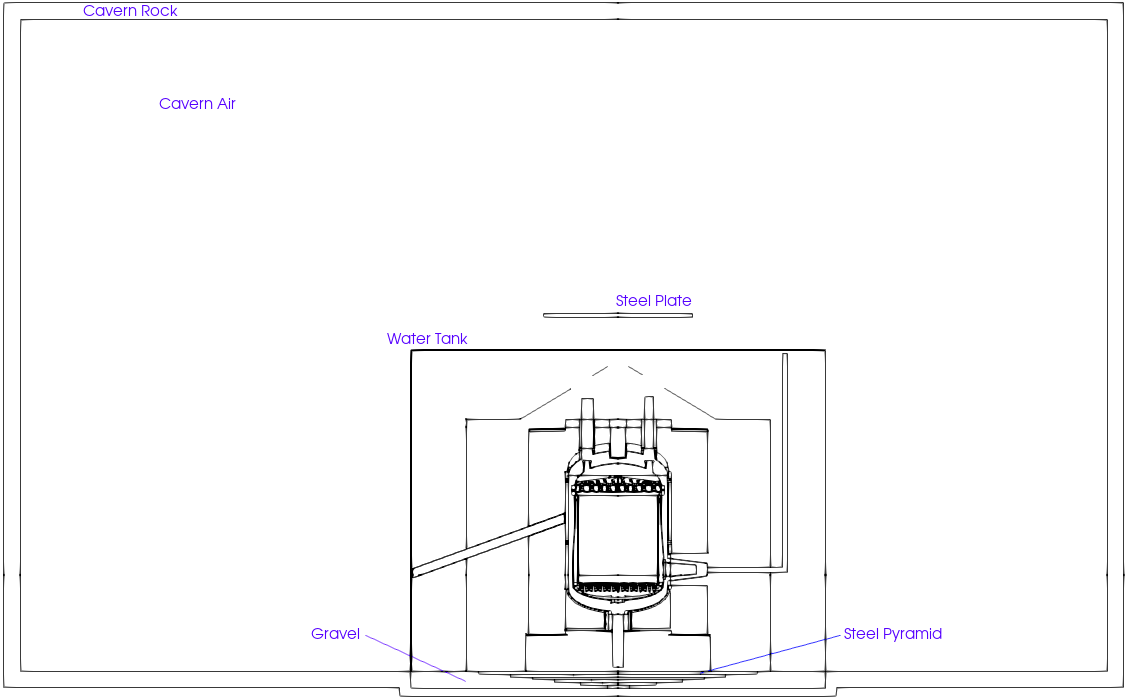
\includegraphics[width=\textwidth]{Figures/Geometry/cavern_geometry_with_markings.png}
\centering
\caption{LZ detector geometry slice with additional cavern geometry as implemented in GEANT4. OD PMTs are not seen present as they do not lie in this plane.}
\label{fig:Cavern_Geometry}
\end{figure}

\par
A generator for these cavern $\gamma$s has existed for some time \cite{rg_generator_ref}, but it has a number of flaws.
Firstly, no $\gamma$s below 2 MeV were included.
This meant that $^{40}K$ was not included and there was a bias to higher energy events and therefore a higher rate.
The previous generator was created using a GEANT4.9.5 while the rest of the simulation chain had moved on to GEANT4.10.3.p02. 
Finally, significant portions of the detector geometry had been updated to reflect more closely the final design. 
This motivated the creation of an updated generator.

\par
The parameters of the new generator are shown in \autoref{tab:cavern_gamma_generator_parameters} and a comparison of the energy distribution of the old and new generators is shown in \autoref{fig:cavern_gamma_energy_distribution}.
Although it can be seen that the previous generators had a maximum $\gamma$ energy of 10 MeV, it also highlights a significant change between GEANT4.9.5 and GEANT4.10.3.p02, namely an increased rate above 9 MeV.
These $\gamma$s are predominately from ($\alpha$,$\gamma$) reactions such as ${}^{17}$O$ + \alpha \to {}^{20}$Ne$ + \gamma$, where a decay $\alpha$ is captured by a nucleus in the rock.
As these higher energy $\gamma$s are able to travel further into the detector they are more likely to reach the TPC.
Conversely, they may produce large signals in the OD which would trigger a veto, reducing the detector livetime.
Since GEANT4.10.3.p02, there have been new studies of the ($\alpha$,$\gamma$) cross-section in other underground laboratories, such as in \cite{cavern_gammas_in_Soudan_mine_ref}.
Generally, very little attention has been given to ($\alpha$,$\gamma$) rates, and so it is possible that the observed rate may differ significantly from that shown here. 
In \autoref{fig:cavern_gamma_energy_distribution} the largest difference is at high energies, as was shown in the Sudan Mine \cite{cavern_gammas_in_Soudan_mine_ref}, the rate of sub-6MeV $\gamma$s may also change significantly. 
There is however evidence that the cross-sections used by GEANT4 - which uses the statistical method from TALYS \cite{talys_ref} - has a large uncertainty for ${}^{17}$O$ + \alpha \to {}^{20}$Ne$ + n$ \cite{alpha_gamma_statistical_error_ref}.
It has been suggested that the rate of $\gamma$'s above 2 MeV from ($\alpha$,$\gamma$) reactions being 5 orders of magnitude higher than expected in GEANT4 simulations \cite{soudanmine_counter_point_ref, alpha_gamma_reactions_ref}.
This is explored on LZ data in \autoref{sec:od_analysis_backgrounds}.

\par
The livetime ($l$) for a simulation can be determined then by $l_{\text{simulation}} = \frac{\text{n.} \gamma_{\text{simulated}}}{\text{n.} \gamma_{\text{generator}}} * \text{l}_{\text{generator}}$
In short, this means that every $\gamma$ in the generator represents roughly 130000 decays from the rock, and so is a significant computational saving on repeated simulations.


\begin{table}
    \centering
    \begin{tabular}{c|c|c|c}
        Generator    & Activity (Bq/kg)   & Boost per surface & Generator livetime (days)  \\ \hline
        ${}^{40}K$   & 216 $\pm$ 60.1     & 28                & 57.72                      \\
        ${}^{238}U$  & 29.1 $\pm$ 15.2    & 34                & 60.26                      \\
        ${}^{232}Th$ & 12.5 $\pm$ 5.0     & 70                & 60.66
    \end{tabular}
    \caption{Parameters used in generator creation. Activity rates are from \cite{LZ_Gamma_Ray_Background_ref}.}
    \label{tab:cavern_gamma_generator_parameters}
\end{table}


\begin{figure}[!htbp]%
\centering
\begin{tikzpicture}
\centering
    \begin{groupplot}[%view={0}{90},
    group style = {group size = 2 by 1,
                   horizontal sep=1.0cm}]
    \nextgroupplot[
            xlabel=Energy (keV),
            ylabel=Rate (Hz/15keV),
            width=0.5\textwidth, height=8cm,
            xmin=0, xmax=14000,
            minor y tick num=8,
            ymode=log, ymin=1e-6, ymax=10,
            grid=major,]
            \addplot[green, mark=none]
                    table [x=Bins,y=Weights]
                    {Data/Simulation_Analysis/Cavern_Gammas/old_gamma_generator_th232.dat};
            \addplot[blue, mark=none]
                    table [x=Bins,y=Weights]
                    {Data/Simulation_Analysis/Cavern_Gammas/old_gamma_generator_u238.dat};

        \nextgroupplot[
            xlabel=Energy (keV),
            width=0.5\textwidth, height=8cm,
            xmin=0, xmax=14000,
            yticklabel pos=right,
            minor y tick num=8,
            ymode=log, ymin=1e-6, ymax=10,
            grid=major,
            legend style = { column sep = 10pt, legend columns = -1, legend to name = Cavern_Gamma_CommonLegend,}]
            \addplot[green, mark=none]
                    table [x=Bins,y=Weights]
                    {Data/Simulation_Analysis/Cavern_Gammas/new_gamma_generator_th232.dat};
            \addplot[blue, mark=none]
                    table [x=Bins,y=Weights]
                    {Data/Simulation_Analysis/Cavern_Gammas/new_gamma_generator_u238.dat};
            \addplot[red, mark=none]
                    table [x=Bins,y=Weights]
                    {Data/Simulation_Analysis/Cavern_Gammas/new_gamma_generator_k40.dat};
            \legend{${}^{232}Th$, ${}^{238}U$, ${}^{40}K$}
            
    \end{groupplot}
    \node at ($(group c2r1) - (group c1r1) + (-0.5cm, 5.0cm)$) {\ref{Cavern_Gamma_CommonLegend}};
\end{tikzpicture}
\caption{Generator $\gamma$ energies. \textbf{Left:} Previous generator. \textbf{Right:} This work.}
\label{fig:cavern_gamma_energy_distribution}
\end{figure}


\par
During the comparison between the two generator versions, it was noticed that the previous generator had not been created correctly.
This caused a bias in the $\gamma$ distribution to the top of the detector, as the generator surface did not cover the sides of the detector adequately.
The most significant effect on this would have been in any dark matter sensitivity study, such as \cite{lz_simulations_ref}, where the fiducial volume may have had to of changed size if external $\gamma$ events were originating from other locations.
The discovery of this was made possible by the geometry visualisation which the author pioneered within the LZ collaboration.

\par
The energy deposit distribution from simulations using the updated generator is shown in \autoref{fig:cavern_gamma_position_distribution}.
The most significant contribution to the rate is in the bottom of the Outer Detector side tanks, and events which enter the TPC enter from the sides as well as the top and bottom\footnote{In the previous generator $\gamma$ would only enter the TPC from the top.}.

\begin{figure}
    \centering
    \resizebox{\textwidth}{!}{
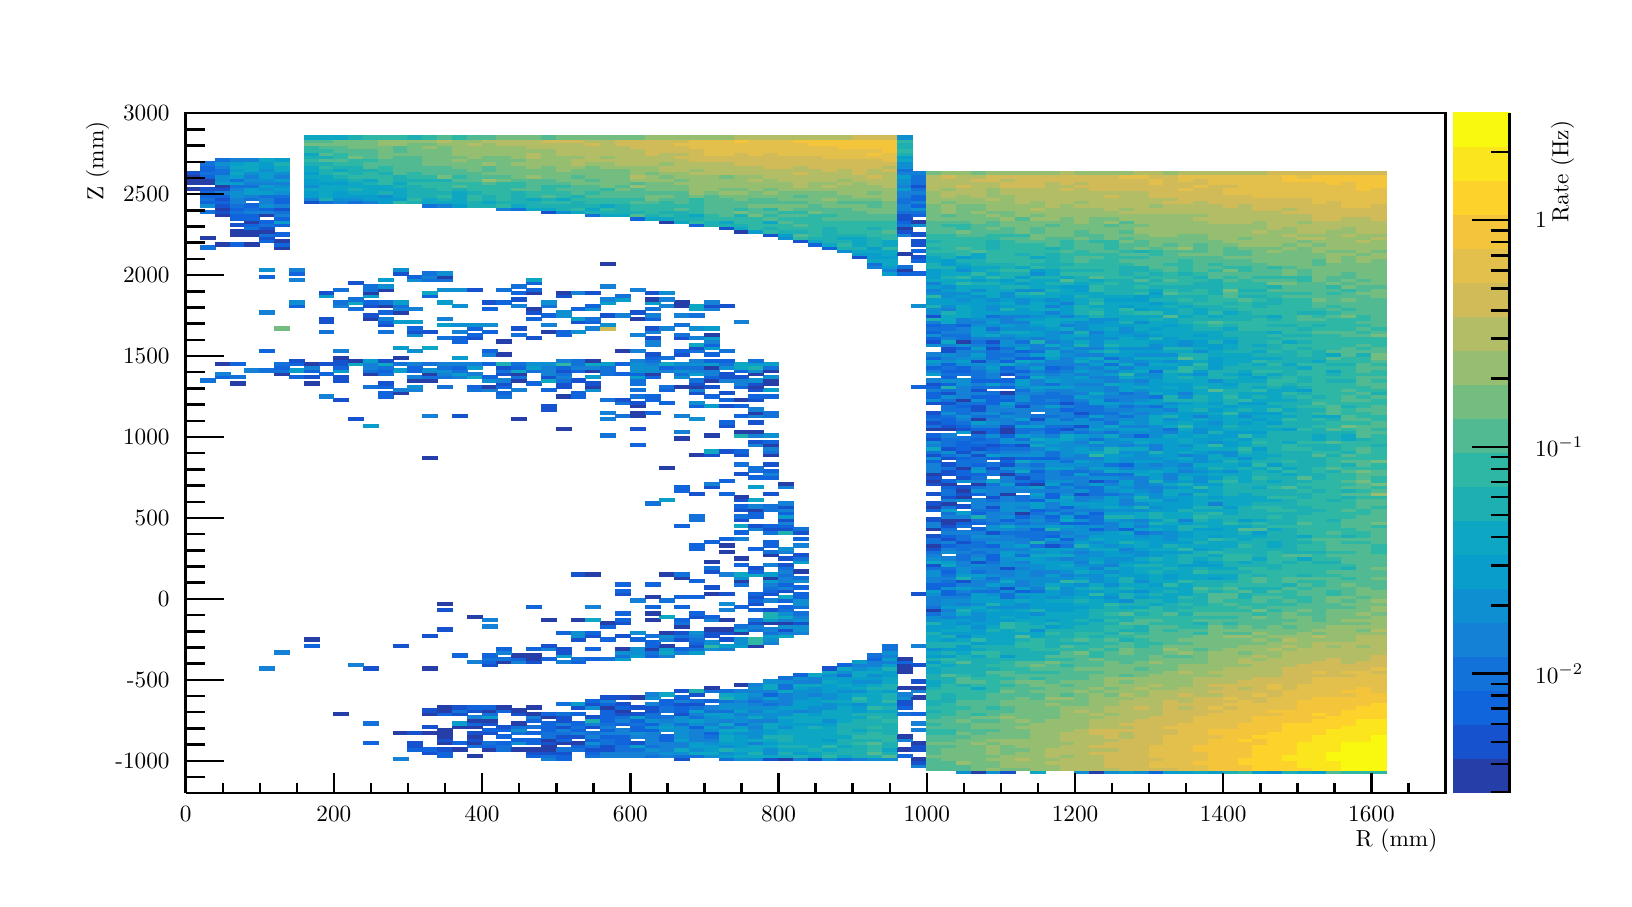
\begin{tikzpicture}
\pgfdeclareplotmark{cross} {
\pgfpathmoveto{\pgfpoint{-0.3\pgfplotmarksize}{\pgfplotmarksize}}
\pgfpathlineto{\pgfpoint{+0.3\pgfplotmarksize}{\pgfplotmarksize}}
\pgfpathlineto{\pgfpoint{+0.3\pgfplotmarksize}{0.3\pgfplotmarksize}}
\pgfpathlineto{\pgfpoint{+1\pgfplotmarksize}{0.3\pgfplotmarksize}}
\pgfpathlineto{\pgfpoint{+1\pgfplotmarksize}{-0.3\pgfplotmarksize}}
\pgfpathlineto{\pgfpoint{+0.3\pgfplotmarksize}{-0.3\pgfplotmarksize}}
\pgfpathlineto{\pgfpoint{+0.3\pgfplotmarksize}{-1.\pgfplotmarksize}}
\pgfpathlineto{\pgfpoint{-0.3\pgfplotmarksize}{-1.\pgfplotmarksize}}
\pgfpathlineto{\pgfpoint{-0.3\pgfplotmarksize}{-0.3\pgfplotmarksize}}
\pgfpathlineto{\pgfpoint{-1.\pgfplotmarksize}{-0.3\pgfplotmarksize}}
\pgfpathlineto{\pgfpoint{-1.\pgfplotmarksize}{0.3\pgfplotmarksize}}
\pgfpathlineto{\pgfpoint{-0.3\pgfplotmarksize}{0.3\pgfplotmarksize}}
\pgfpathclose
\pgfusepathqstroke
}
\pgfdeclareplotmark{cross*} {
\pgfpathmoveto{\pgfpoint{-0.3\pgfplotmarksize}{\pgfplotmarksize}}
\pgfpathlineto{\pgfpoint{+0.3\pgfplotmarksize}{\pgfplotmarksize}}
\pgfpathlineto{\pgfpoint{+0.3\pgfplotmarksize}{0.3\pgfplotmarksize}}
\pgfpathlineto{\pgfpoint{+1\pgfplotmarksize}{0.3\pgfplotmarksize}}
\pgfpathlineto{\pgfpoint{+1\pgfplotmarksize}{-0.3\pgfplotmarksize}}
\pgfpathlineto{\pgfpoint{+0.3\pgfplotmarksize}{-0.3\pgfplotmarksize}}
\pgfpathlineto{\pgfpoint{+0.3\pgfplotmarksize}{-1.\pgfplotmarksize}}
\pgfpathlineto{\pgfpoint{-0.3\pgfplotmarksize}{-1.\pgfplotmarksize}}
\pgfpathlineto{\pgfpoint{-0.3\pgfplotmarksize}{-0.3\pgfplotmarksize}}
\pgfpathlineto{\pgfpoint{-1.\pgfplotmarksize}{-0.3\pgfplotmarksize}}
\pgfpathlineto{\pgfpoint{-1.\pgfplotmarksize}{0.3\pgfplotmarksize}}
\pgfpathlineto{\pgfpoint{-0.3\pgfplotmarksize}{0.3\pgfplotmarksize}}
\pgfpathclose
\pgfusepathqfillstroke
}
\pgfdeclareplotmark{newstar} {
\pgfpathmoveto{\pgfqpoint{0pt}{\pgfplotmarksize}}
\pgfpathlineto{\pgfqpointpolar{44}{0.5\pgfplotmarksize}}
\pgfpathlineto{\pgfqpointpolar{18}{\pgfplotmarksize}}
\pgfpathlineto{\pgfqpointpolar{-20}{0.5\pgfplotmarksize}}
\pgfpathlineto{\pgfqpointpolar{-54}{\pgfplotmarksize}}
\pgfpathlineto{\pgfqpointpolar{-90}{0.5\pgfplotmarksize}}
\pgfpathlineto{\pgfqpointpolar{234}{\pgfplotmarksize}}
\pgfpathlineto{\pgfqpointpolar{198}{0.5\pgfplotmarksize}}
\pgfpathlineto{\pgfqpointpolar{162}{\pgfplotmarksize}}
\pgfpathlineto{\pgfqpointpolar{134}{0.5\pgfplotmarksize}}
\pgfpathclose
\pgfusepathqstroke
}
\pgfdeclareplotmark{newstar*} {
\pgfpathmoveto{\pgfqpoint{0pt}{\pgfplotmarksize}}
\pgfpathlineto{\pgfqpointpolar{44}{0.5\pgfplotmarksize}}
\pgfpathlineto{\pgfqpointpolar{18}{\pgfplotmarksize}}
\pgfpathlineto{\pgfqpointpolar{-20}{0.5\pgfplotmarksize}}
\pgfpathlineto{\pgfqpointpolar{-54}{\pgfplotmarksize}}
\pgfpathlineto{\pgfqpointpolar{-90}{0.5\pgfplotmarksize}}
\pgfpathlineto{\pgfqpointpolar{234}{\pgfplotmarksize}}
\pgfpathlineto{\pgfqpointpolar{198}{0.5\pgfplotmarksize}}
\pgfpathlineto{\pgfqpointpolar{162}{\pgfplotmarksize}}
\pgfpathlineto{\pgfqpointpolar{134}{0.5\pgfplotmarksize}}
\pgfpathclose
\pgfusepathqfillstroke
}
\definecolor{c}{rgb}{1,1,1};
\draw [color=c, fill=c] (0,0) rectangle (20,10.7945);
\draw [color=c, fill=c] (2,1.07945) rectangle (18,9.71501);
\definecolor{c}{rgb}{0,0,0};
\draw [c,line width=0.9] (2,1.07945) -- (2,9.71501) -- (18,9.71501) -- (18,1.07945) -- (2,1.07945);
\definecolor{c}{rgb}{1,1,1};
\draw [color=c, fill=c] (2,1.07945) rectangle (18,9.71501);
\definecolor{c}{rgb}{0,0,0};
\draw [c,line width=0.9] (2,1.07945) -- (2,9.71501) -- (18,9.71501) -- (18,1.07945) -- (2,1.07945);
\definecolor{c}{rgb}{0.0557375,0.560081,0.819366};
\draw [color=c, fill=c] (11.7882,1.32618) rectangle (11.9765,1.3673);
\definecolor{c}{rgb}{0.150523,0.241303,0.660565};
\draw [color=c, fill=c] (11.9765,1.32618) rectangle (12.1647,1.3673);
\definecolor{c}{rgb}{0.0557375,0.560081,0.819366};
\draw [color=c, fill=c] (12.1647,1.32618) rectangle (12.3529,1.3673);
\definecolor{c}{rgb}{0.0880387,0.322448,0.802768};
\draw [color=c, fill=c] (12.3529,1.32618) rectangle (12.5412,1.3673);
\definecolor{c}{rgb}{0.0526375,0.656131,0.763481};
\draw [color=c, fill=c] (12.7294,1.32618) rectangle (12.9176,1.3673);
\definecolor{c}{rgb}{0.0557375,0.560081,0.819366};
\draw [color=c, fill=c] (13.2941,1.32618) rectangle (13.4824,1.3673);
\definecolor{c}{rgb}{0.150523,0.241303,0.660565};
\draw [color=c, fill=c] (13.4824,1.32618) rectangle (13.6706,1.3673);
\definecolor{c}{rgb}{0.0557375,0.560081,0.819366};
\draw [color=c, fill=c] (13.6706,1.32618) rectangle (13.8588,1.3673);
\definecolor{c}{rgb}{0.033475,0.616063,0.800231};
\draw [color=c, fill=c] (13.8588,1.32618) rectangle (14.0471,1.3673);
\definecolor{c}{rgb}{0.0557375,0.560081,0.819366};
\draw [color=c, fill=c] (14.0471,1.32618) rectangle (14.2353,1.3673);
\definecolor{c}{rgb}{0.0633125,0.391444,0.861859};
\draw [color=c, fill=c] (14.2353,1.32618) rectangle (14.4235,1.3673);
\definecolor{c}{rgb}{0.033475,0.616063,0.800231};
\draw [color=c, fill=c] (14.4235,1.32618) rectangle (14.6118,1.3673);
\draw [color=c, fill=c] (14.6118,1.32618) rectangle (14.8,1.3673);
\definecolor{c}{rgb}{0.0526375,0.656131,0.763481};
\draw [color=c, fill=c] (14.8,1.32618) rectangle (14.9882,1.3673);
\definecolor{c}{rgb}{0.033475,0.616063,0.800231};
\draw [color=c, fill=c] (14.9882,1.32618) rectangle (15.1765,1.3673);
\definecolor{c}{rgb}{0.116419,0.686966,0.702991};
\draw [color=c, fill=c] (15.1765,1.32618) rectangle (15.3647,1.3673);
\definecolor{c}{rgb}{0.1802,0.7178,0.6425};
\draw [color=c, fill=c] (15.3647,1.32618) rectangle (15.5529,1.3673);
\definecolor{c}{rgb}{0.033475,0.616063,0.800231};
\draw [color=c, fill=c] (15.5529,1.32618) rectangle (15.7412,1.3673);
\definecolor{c}{rgb}{0.0557375,0.560081,0.819366};
\draw [color=c, fill=c] (15.7412,1.32618) rectangle (15.9294,1.3673);
\definecolor{c}{rgb}{0.116419,0.686966,0.702991};
\draw [color=c, fill=c] (15.9294,1.32618) rectangle (16.1176,1.3673);
\definecolor{c}{rgb}{0.0526375,0.656131,0.763481};
\draw [color=c, fill=c] (16.1176,1.32618) rectangle (16.3059,1.3673);
\definecolor{c}{rgb}{0.033475,0.616063,0.800231};
\draw [color=c, fill=c] (16.3059,1.32618) rectangle (16.4941,1.3673);
\definecolor{c}{rgb}{0.322347,0.730556,0.570878};
\draw [color=c, fill=c] (16.4941,1.32618) rectangle (16.6824,1.3673);
\definecolor{c}{rgb}{0.1802,0.7178,0.6425};
\draw [color=c, fill=c] (16.6824,1.32618) rectangle (16.8706,1.3673);
\draw [color=c, fill=c] (16.8706,1.32618) rectangle (17.0588,1.3673);
\draw [color=c, fill=c] (17.0588,1.32618) rectangle (17.2471,1.3673);
\definecolor{c}{rgb}{0.322347,0.730556,0.570878};
\draw [color=c, fill=c] (11.4118,1.3673) rectangle (11.6,1.40842);
\draw [color=c, fill=c] (11.6,1.3673) rectangle (11.7882,1.40842);
\draw [color=c, fill=c] (11.7882,1.3673) rectangle (11.9765,1.40842);
\definecolor{c}{rgb}{0.453559,0.742331,0.504766};
\draw [color=c, fill=c] (11.9765,1.3673) rectangle (12.1647,1.40842);
\definecolor{c}{rgb}{0.584194,0.746125,0.444394};
\draw [color=c, fill=c] (12.1647,1.3673) rectangle (12.3529,1.40842);
\definecolor{c}{rgb}{0.453559,0.742331,0.504766};
\draw [color=c, fill=c] (12.3529,1.3673) rectangle (12.5412,1.40842);
\draw [color=c, fill=c] (12.5412,1.3673) rectangle (12.7294,1.40842);
\definecolor{c}{rgb}{0.584194,0.746125,0.444394};
\draw [color=c, fill=c] (12.7294,1.3673) rectangle (12.9176,1.40842);
\draw [color=c, fill=c] (12.9176,1.3673) rectangle (13.1059,1.40842);
\definecolor{c}{rgb}{0.701397,0.739462,0.397147};
\draw [color=c, fill=c] (13.1059,1.3673) rectangle (13.2941,1.40842);
\draw [color=c, fill=c] (13.2941,1.3673) rectangle (13.4824,1.40842);
\draw [color=c, fill=c] (13.4824,1.3673) rectangle (13.6706,1.40842);
\draw [color=c, fill=c] (13.6706,1.3673) rectangle (13.8588,1.40842);
\definecolor{c}{rgb}{0.8186,0.7328,0.3499};
\draw [color=c, fill=c] (13.8588,1.3673) rectangle (14.0471,1.40842);
\draw [color=c, fill=c] (14.0471,1.3673) rectangle (14.2353,1.40842);
\draw [color=c, fill=c] (14.2353,1.3673) rectangle (14.4235,1.40842);
\draw [color=c, fill=c] (14.4235,1.3673) rectangle (14.6118,1.40842);
\definecolor{c}{rgb}{0.884975,0.752825,0.292488};
\draw [color=c, fill=c] (14.6118,1.3673) rectangle (14.8,1.40842);
\draw [color=c, fill=c] (14.8,1.3673) rectangle (14.9882,1.40842);
\definecolor{c}{rgb}{0.956881,0.774519,0.230291};
\draw [color=c, fill=c] (14.9882,1.3673) rectangle (15.1765,1.40842);
\draw [color=c, fill=c] (15.1765,1.3673) rectangle (15.3647,1.40842);
\draw [color=c, fill=c] (15.3647,1.3673) rectangle (15.5529,1.40842);
\definecolor{c}{rgb}{0.992,0.823138,0.170006};
\draw [color=c, fill=c] (15.5529,1.3673) rectangle (15.7412,1.40842);
\draw [color=c, fill=c] (15.7412,1.3673) rectangle (15.9294,1.40842);
\draw [color=c, fill=c] (15.9294,1.3673) rectangle (16.1176,1.40842);
\draw [color=c, fill=c] (16.1176,1.3673) rectangle (16.3059,1.40842);
\definecolor{c}{rgb}{0.9842,0.903169,0.111953};
\draw [color=c, fill=c] (16.3059,1.3673) rectangle (16.4941,1.40842);
\draw [color=c, fill=c] (16.4941,1.3673) rectangle (16.6824,1.40842);
\definecolor{c}{rgb}{0.977,0.977044,0.0583656};
\draw [color=c, fill=c] (16.6824,1.3673) rectangle (16.8706,1.40842);
\draw [color=c, fill=c] (16.8706,1.3673) rectangle (17.0588,1.40842);
\draw [color=c, fill=c] (17.0588,1.3673) rectangle (17.2471,1.40842);
\definecolor{c}{rgb}{0.078,0.5041,0.8385};
\draw [color=c, fill=c] (11.2235,1.40842) rectangle (11.4118,1.44954);
\definecolor{c}{rgb}{0.322347,0.730556,0.570878};
\draw [color=c, fill=c] (11.4118,1.40842) rectangle (11.6,1.44954);
\draw [color=c, fill=c] (11.6,1.40842) rectangle (11.7882,1.44954);
\draw [color=c, fill=c] (11.7882,1.40842) rectangle (11.9765,1.44954);
\definecolor{c}{rgb}{0.453559,0.742331,0.504766};
\draw [color=c, fill=c] (11.9765,1.40842) rectangle (12.1647,1.44954);
\draw [color=c, fill=c] (12.1647,1.40842) rectangle (12.3529,1.44954);
\definecolor{c}{rgb}{0.584194,0.746125,0.444394};
\draw [color=c, fill=c] (12.3529,1.40842) rectangle (12.5412,1.44954);
\draw [color=c, fill=c] (12.5412,1.40842) rectangle (12.7294,1.44954);
\draw [color=c, fill=c] (12.7294,1.40842) rectangle (12.9176,1.44954);
\draw [color=c, fill=c] (12.9176,1.40842) rectangle (13.1059,1.44954);
\definecolor{c}{rgb}{0.701397,0.739462,0.397147};
\draw [color=c, fill=c] (13.1059,1.40842) rectangle (13.2941,1.44954);
\draw [color=c, fill=c] (13.2941,1.40842) rectangle (13.4824,1.44954);
\draw [color=c, fill=c] (13.4824,1.40842) rectangle (13.6706,1.44954);
\definecolor{c}{rgb}{0.8186,0.7328,0.3499};
\draw [color=c, fill=c] (13.6706,1.40842) rectangle (13.8588,1.44954);
\draw [color=c, fill=c] (13.8588,1.40842) rectangle (14.0471,1.44954);
\draw [color=c, fill=c] (14.0471,1.40842) rectangle (14.2353,1.44954);
\definecolor{c}{rgb}{0.884975,0.752825,0.292488};
\draw [color=c, fill=c] (14.2353,1.40842) rectangle (14.4235,1.44954);
\draw [color=c, fill=c] (14.4235,1.40842) rectangle (14.6118,1.44954);
\draw [color=c, fill=c] (14.6118,1.40842) rectangle (14.8,1.44954);
\draw [color=c, fill=c] (14.8,1.40842) rectangle (14.9882,1.44954);
\definecolor{c}{rgb}{0.956881,0.774519,0.230291};
\draw [color=c, fill=c] (14.9882,1.40842) rectangle (15.1765,1.44954);
\draw [color=c, fill=c] (15.1765,1.40842) rectangle (15.3647,1.44954);
\draw [color=c, fill=c] (15.3647,1.40842) rectangle (15.5529,1.44954);
\definecolor{c}{rgb}{0.992,0.823138,0.170006};
\draw [color=c, fill=c] (15.5529,1.40842) rectangle (15.7412,1.44954);
\draw [color=c, fill=c] (15.7412,1.40842) rectangle (15.9294,1.44954);
\draw [color=c, fill=c] (15.9294,1.40842) rectangle (16.1176,1.44954);
\definecolor{c}{rgb}{0.9842,0.903169,0.111953};
\draw [color=c, fill=c] (16.1176,1.40842) rectangle (16.3059,1.44954);
\draw [color=c, fill=c] (16.3059,1.40842) rectangle (16.4941,1.44954);
\draw [color=c, fill=c] (16.4941,1.40842) rectangle (16.6824,1.44954);
\definecolor{c}{rgb}{0.977,0.977044,0.0583656};
\draw [color=c, fill=c] (16.6824,1.40842) rectangle (16.8706,1.44954);
\draw [color=c, fill=c] (16.8706,1.40842) rectangle (17.0588,1.44954);
\draw [color=c, fill=c] (17.0588,1.40842) rectangle (17.2471,1.44954);
\definecolor{c}{rgb}{0.0880387,0.322448,0.802768};
\draw [color=c, fill=c] (11.2235,1.44954) rectangle (11.4118,1.49066);
\definecolor{c}{rgb}{0.322347,0.730556,0.570878};
\draw [color=c, fill=c] (11.4118,1.44954) rectangle (11.6,1.49066);
\draw [color=c, fill=c] (11.6,1.44954) rectangle (11.7882,1.49066);
\definecolor{c}{rgb}{0.584194,0.746125,0.444394};
\draw [color=c, fill=c] (11.7882,1.44954) rectangle (11.9765,1.49066);
\definecolor{c}{rgb}{0.453559,0.742331,0.504766};
\draw [color=c, fill=c] (11.9765,1.44954) rectangle (12.1647,1.49066);
\draw [color=c, fill=c] (12.1647,1.44954) rectangle (12.3529,1.49066);
\definecolor{c}{rgb}{0.584194,0.746125,0.444394};
\draw [color=c, fill=c] (12.3529,1.44954) rectangle (12.5412,1.49066);
\draw [color=c, fill=c] (12.5412,1.44954) rectangle (12.7294,1.49066);
\draw [color=c, fill=c] (12.7294,1.44954) rectangle (12.9176,1.49066);
\definecolor{c}{rgb}{0.701397,0.739462,0.397147};
\draw [color=c, fill=c] (12.9176,1.44954) rectangle (13.1059,1.49066);
\draw [color=c, fill=c] (13.1059,1.44954) rectangle (13.2941,1.49066);
\draw [color=c, fill=c] (13.2941,1.44954) rectangle (13.4824,1.49066);
\draw [color=c, fill=c] (13.4824,1.44954) rectangle (13.6706,1.49066);
\definecolor{c}{rgb}{0.8186,0.7328,0.3499};
\draw [color=c, fill=c] (13.6706,1.44954) rectangle (13.8588,1.49066);
\draw [color=c, fill=c] (13.8588,1.44954) rectangle (14.0471,1.49066);
\draw [color=c, fill=c] (14.0471,1.44954) rectangle (14.2353,1.49066);
\definecolor{c}{rgb}{0.884975,0.752825,0.292488};
\draw [color=c, fill=c] (14.2353,1.44954) rectangle (14.4235,1.49066);
\draw [color=c, fill=c] (14.4235,1.44954) rectangle (14.6118,1.49066);
\draw [color=c, fill=c] (14.6118,1.44954) rectangle (14.8,1.49066);
\definecolor{c}{rgb}{0.956881,0.774519,0.230291};
\draw [color=c, fill=c] (14.8,1.44954) rectangle (14.9882,1.49066);
\draw [color=c, fill=c] (14.9882,1.44954) rectangle (15.1765,1.49066);
\draw [color=c, fill=c] (15.1765,1.44954) rectangle (15.3647,1.49066);
\definecolor{c}{rgb}{0.992,0.823138,0.170006};
\draw [color=c, fill=c] (15.3647,1.44954) rectangle (15.5529,1.49066);
\draw [color=c, fill=c] (15.5529,1.44954) rectangle (15.7412,1.49066);
\draw [color=c, fill=c] (15.7412,1.44954) rectangle (15.9294,1.49066);
\draw [color=c, fill=c] (15.9294,1.44954) rectangle (16.1176,1.49066);
\definecolor{c}{rgb}{0.9842,0.903169,0.111953};
\draw [color=c, fill=c] (16.1176,1.44954) rectangle (16.3059,1.49066);
\draw [color=c, fill=c] (16.3059,1.44954) rectangle (16.4941,1.49066);
\draw [color=c, fill=c] (16.4941,1.44954) rectangle (16.6824,1.49066);
\definecolor{c}{rgb}{0.977,0.977044,0.0583656};
\draw [color=c, fill=c] (16.6824,1.44954) rectangle (16.8706,1.49066);
\draw [color=c, fill=c] (16.8706,1.44954) rectangle (17.0588,1.49066);
\draw [color=c, fill=c] (17.0588,1.44954) rectangle (17.2471,1.49066);
\definecolor{c}{rgb}{0.078,0.5041,0.8385};
\draw [color=c, fill=c] (4.63529,1.49066) rectangle (4.82353,1.53178);
\draw [color=c, fill=c] (6.51765,1.49066) rectangle (6.70588,1.53178);
\definecolor{c}{rgb}{0.0633125,0.391444,0.861859};
\draw [color=c, fill=c] (6.70588,1.49066) rectangle (6.89412,1.53178);
\definecolor{c}{rgb}{0.0880387,0.322448,0.802768};
\draw [color=c, fill=c] (8.21176,1.49066) rectangle (8.4,1.53178);
\definecolor{c}{rgb}{0.0703625,0.445519,0.850647};
\draw [color=c, fill=c] (8.77647,1.49066) rectangle (8.96471,1.53178);
\definecolor{c}{rgb}{0.0557375,0.560081,0.819366};
\draw [color=c, fill=c] (8.96471,1.49066) rectangle (9.15294,1.53178);
\draw [color=c, fill=c] (9.15294,1.49066) rectangle (9.34118,1.53178);
\definecolor{c}{rgb}{0.0880387,0.322448,0.802768};
\draw [color=c, fill=c] (9.34118,1.49066) rectangle (9.52941,1.53178);
\definecolor{c}{rgb}{0.150523,0.241303,0.660565};
\draw [color=c, fill=c] (9.52941,1.49066) rectangle (9.71765,1.53178);
\definecolor{c}{rgb}{0.078,0.5041,0.8385};
\draw [color=c, fill=c] (9.71765,1.49066) rectangle (9.90588,1.53178);
\definecolor{c}{rgb}{0.0880387,0.322448,0.802768};
\draw [color=c, fill=c] (9.90588,1.49066) rectangle (10.0941,1.53178);
\definecolor{c}{rgb}{0.0557375,0.560081,0.819366};
\draw [color=c, fill=c] (10.0941,1.49066) rectangle (10.2824,1.53178);
\definecolor{c}{rgb}{0.0703625,0.445519,0.850647};
\draw [color=c, fill=c] (10.2824,1.49066) rectangle (10.4706,1.53178);
\definecolor{c}{rgb}{0.078,0.5041,0.8385};
\draw [color=c, fill=c] (10.4706,1.49066) rectangle (10.6588,1.53178);
\definecolor{c}{rgb}{0.0557375,0.560081,0.819366};
\draw [color=c, fill=c] (10.6588,1.49066) rectangle (10.8471,1.53178);
\draw [color=c, fill=c] (10.8471,1.49066) rectangle (11.0353,1.53178);
\definecolor{c}{rgb}{0.150523,0.241303,0.660565};
\draw [color=c, fill=c] (11.2235,1.49066) rectangle (11.4118,1.53178);
\definecolor{c}{rgb}{0.322347,0.730556,0.570878};
\draw [color=c, fill=c] (11.4118,1.49066) rectangle (11.6,1.53178);
\definecolor{c}{rgb}{0.453559,0.742331,0.504766};
\draw [color=c, fill=c] (11.6,1.49066) rectangle (11.7882,1.53178);
\draw [color=c, fill=c] (11.7882,1.49066) rectangle (11.9765,1.53178);
\draw [color=c, fill=c] (11.9765,1.49066) rectangle (12.1647,1.53178);
\definecolor{c}{rgb}{0.584194,0.746125,0.444394};
\draw [color=c, fill=c] (12.1647,1.49066) rectangle (12.3529,1.53178);
\draw [color=c, fill=c] (12.3529,1.49066) rectangle (12.5412,1.53178);
\definecolor{c}{rgb}{0.701397,0.739462,0.397147};
\draw [color=c, fill=c] (12.5412,1.49066) rectangle (12.7294,1.53178);
\definecolor{c}{rgb}{0.584194,0.746125,0.444394};
\draw [color=c, fill=c] (12.7294,1.49066) rectangle (12.9176,1.53178);
\draw [color=c, fill=c] (12.9176,1.49066) rectangle (13.1059,1.53178);
\definecolor{c}{rgb}{0.701397,0.739462,0.397147};
\draw [color=c, fill=c] (13.1059,1.49066) rectangle (13.2941,1.53178);
\draw [color=c, fill=c] (13.2941,1.49066) rectangle (13.4824,1.53178);
\draw [color=c, fill=c] (13.4824,1.49066) rectangle (13.6706,1.53178);
\definecolor{c}{rgb}{0.8186,0.7328,0.3499};
\draw [color=c, fill=c] (13.6706,1.49066) rectangle (13.8588,1.53178);
\draw [color=c, fill=c] (13.8588,1.49066) rectangle (14.0471,1.53178);
\draw [color=c, fill=c] (14.0471,1.49066) rectangle (14.2353,1.53178);
\draw [color=c, fill=c] (14.2353,1.49066) rectangle (14.4235,1.53178);
\definecolor{c}{rgb}{0.884975,0.752825,0.292488};
\draw [color=c, fill=c] (14.4235,1.49066) rectangle (14.6118,1.53178);
\draw [color=c, fill=c] (14.6118,1.49066) rectangle (14.8,1.53178);
\draw [color=c, fill=c] (14.8,1.49066) rectangle (14.9882,1.53178);
\definecolor{c}{rgb}{0.956881,0.774519,0.230291};
\draw [color=c, fill=c] (14.9882,1.49066) rectangle (15.1765,1.53178);
\draw [color=c, fill=c] (15.1765,1.49066) rectangle (15.3647,1.53178);
\definecolor{c}{rgb}{0.992,0.823138,0.170006};
\draw [color=c, fill=c] (15.3647,1.49066) rectangle (15.5529,1.53178);
\draw [color=c, fill=c] (15.5529,1.49066) rectangle (15.7412,1.53178);
\draw [color=c, fill=c] (15.7412,1.49066) rectangle (15.9294,1.53178);
\definecolor{c}{rgb}{0.9842,0.903169,0.111953};
\draw [color=c, fill=c] (15.9294,1.49066) rectangle (16.1176,1.53178);
\draw [color=c, fill=c] (16.1176,1.49066) rectangle (16.3059,1.53178);
\draw [color=c, fill=c] (16.3059,1.49066) rectangle (16.4941,1.53178);
\definecolor{c}{rgb}{0.977,0.977044,0.0583656};
\draw [color=c, fill=c] (16.4941,1.49066) rectangle (16.6824,1.53178);
\draw [color=c, fill=c] (16.6824,1.49066) rectangle (16.8706,1.53178);
\draw [color=c, fill=c] (16.8706,1.49066) rectangle (17.0588,1.53178);
\draw [color=c, fill=c] (17.0588,1.49066) rectangle (17.2471,1.53178);
\definecolor{c}{rgb}{0.0633125,0.391444,0.861859};
\draw [color=c, fill=c] (5.2,1.53178) rectangle (5.38824,1.57291);
\definecolor{c}{rgb}{0.150523,0.241303,0.660565};
\draw [color=c, fill=c] (5.57647,1.53178) rectangle (5.76471,1.57291);
\definecolor{c}{rgb}{0.0633125,0.391444,0.861859};
\draw [color=c, fill=c] (6.32941,1.53178) rectangle (6.51765,1.57291);
\definecolor{c}{rgb}{0.0703625,0.445519,0.850647};
\draw [color=c, fill=c] (6.51765,1.53178) rectangle (6.70588,1.57291);
\definecolor{c}{rgb}{0.0633125,0.391444,0.861859};
\draw [color=c, fill=c] (6.70588,1.53178) rectangle (6.89412,1.57291);
\definecolor{c}{rgb}{0.0703625,0.445519,0.850647};
\draw [color=c, fill=c] (7.08235,1.53178) rectangle (7.27059,1.57291);
\definecolor{c}{rgb}{0.078,0.5041,0.8385};
\draw [color=c, fill=c] (7.27059,1.53178) rectangle (7.45882,1.57291);
\draw [color=c, fill=c] (7.45882,1.53178) rectangle (7.64706,1.57291);
\draw [color=c, fill=c] (7.64706,1.53178) rectangle (7.83529,1.57291);
\definecolor{c}{rgb}{0.0703625,0.445519,0.850647};
\draw [color=c, fill=c] (7.83529,1.53178) rectangle (8.02353,1.57291);
\definecolor{c}{rgb}{0.078,0.5041,0.8385};
\draw [color=c, fill=c] (8.02353,1.53178) rectangle (8.21176,1.57291);
\definecolor{c}{rgb}{0.0703625,0.445519,0.850647};
\draw [color=c, fill=c] (8.21176,1.53178) rectangle (8.4,1.57291);
\draw [color=c, fill=c] (8.4,1.53178) rectangle (8.58823,1.57291);
\definecolor{c}{rgb}{0.0557375,0.560081,0.819366};
\draw [color=c, fill=c] (8.58823,1.53178) rectangle (8.77647,1.57291);
\definecolor{c}{rgb}{0.033475,0.616063,0.800231};
\draw [color=c, fill=c] (8.77647,1.53178) rectangle (8.96471,1.57291);
\definecolor{c}{rgb}{0.0526375,0.656131,0.763481};
\draw [color=c, fill=c] (8.96471,1.53178) rectangle (9.15294,1.57291);
\draw [color=c, fill=c] (9.15294,1.53178) rectangle (9.34118,1.57291);
\draw [color=c, fill=c] (9.34118,1.53178) rectangle (9.52941,1.57291);
\draw [color=c, fill=c] (9.52941,1.53178) rectangle (9.71765,1.57291);
\definecolor{c}{rgb}{0.116419,0.686966,0.702991};
\draw [color=c, fill=c] (9.71765,1.53178) rectangle (9.90588,1.57291);
\definecolor{c}{rgb}{0.0526375,0.656131,0.763481};
\draw [color=c, fill=c] (9.90588,1.53178) rectangle (10.0941,1.57291);
\definecolor{c}{rgb}{0.1802,0.7178,0.6425};
\draw [color=c, fill=c] (10.0941,1.53178) rectangle (10.2824,1.57291);
\definecolor{c}{rgb}{0.0526375,0.656131,0.763481};
\draw [color=c, fill=c] (10.2824,1.53178) rectangle (10.4706,1.57291);
\definecolor{c}{rgb}{0.116419,0.686966,0.702991};
\draw [color=c, fill=c] (10.4706,1.53178) rectangle (10.6588,1.57291);
\draw [color=c, fill=c] (10.6588,1.53178) rectangle (10.8471,1.57291);
\definecolor{c}{rgb}{0.322347,0.730556,0.570878};
\draw [color=c, fill=c] (10.8471,1.53178) rectangle (11.0353,1.57291);
\definecolor{c}{rgb}{0.0633125,0.391444,0.861859};
\draw [color=c, fill=c] (11.0353,1.53178) rectangle (11.2235,1.57291);
\definecolor{c}{rgb}{0.453559,0.742331,0.504766};
\draw [color=c, fill=c] (11.4118,1.53178) rectangle (11.6,1.57291);
\draw [color=c, fill=c] (11.6,1.53178) rectangle (11.7882,1.57291);
\draw [color=c, fill=c] (11.7882,1.53178) rectangle (11.9765,1.57291);
\draw [color=c, fill=c] (11.9765,1.53178) rectangle (12.1647,1.57291);
\draw [color=c, fill=c] (12.1647,1.53178) rectangle (12.3529,1.57291);
\definecolor{c}{rgb}{0.584194,0.746125,0.444394};
\draw [color=c, fill=c] (12.3529,1.53178) rectangle (12.5412,1.57291);
\draw [color=c, fill=c] (12.5412,1.53178) rectangle (12.7294,1.57291);
\draw [color=c, fill=c] (12.7294,1.53178) rectangle (12.9176,1.57291);
\definecolor{c}{rgb}{0.701397,0.739462,0.397147};
\draw [color=c, fill=c] (12.9176,1.53178) rectangle (13.1059,1.57291);
\definecolor{c}{rgb}{0.584194,0.746125,0.444394};
\draw [color=c, fill=c] (13.1059,1.53178) rectangle (13.2941,1.57291);
\definecolor{c}{rgb}{0.701397,0.739462,0.397147};
\draw [color=c, fill=c] (13.2941,1.53178) rectangle (13.4824,1.57291);
\draw [color=c, fill=c] (13.4824,1.53178) rectangle (13.6706,1.57291);
\definecolor{c}{rgb}{0.8186,0.7328,0.3499};
\draw [color=c, fill=c] (13.6706,1.53178) rectangle (13.8588,1.57291);
\draw [color=c, fill=c] (13.8588,1.53178) rectangle (14.0471,1.57291);
\draw [color=c, fill=c] (14.0471,1.53178) rectangle (14.2353,1.57291);
\definecolor{c}{rgb}{0.884975,0.752825,0.292488};
\draw [color=c, fill=c] (14.2353,1.53178) rectangle (14.4235,1.57291);
\draw [color=c, fill=c] (14.4235,1.53178) rectangle (14.6118,1.57291);
\draw [color=c, fill=c] (14.6118,1.53178) rectangle (14.8,1.57291);
\draw [color=c, fill=c] (14.8,1.53178) rectangle (14.9882,1.57291);
\definecolor{c}{rgb}{0.956881,0.774519,0.230291};
\draw [color=c, fill=c] (14.9882,1.53178) rectangle (15.1765,1.57291);
\draw [color=c, fill=c] (15.1765,1.53178) rectangle (15.3647,1.57291);
\draw [color=c, fill=c] (15.3647,1.53178) rectangle (15.5529,1.57291);
\definecolor{c}{rgb}{0.992,0.823138,0.170006};
\draw [color=c, fill=c] (15.5529,1.53178) rectangle (15.7412,1.57291);
\draw [color=c, fill=c] (15.7412,1.53178) rectangle (15.9294,1.57291);
\definecolor{c}{rgb}{0.9842,0.903169,0.111953};
\draw [color=c, fill=c] (15.9294,1.53178) rectangle (16.1176,1.57291);
\draw [color=c, fill=c] (16.1176,1.53178) rectangle (16.3059,1.57291);
\draw [color=c, fill=c] (16.3059,1.53178) rectangle (16.4941,1.57291);
\definecolor{c}{rgb}{0.977,0.977044,0.0583656};
\draw [color=c, fill=c] (16.4941,1.53178) rectangle (16.6824,1.57291);
\draw [color=c, fill=c] (16.6824,1.53178) rectangle (16.8706,1.57291);
\draw [color=c, fill=c] (16.8706,1.53178) rectangle (17.0588,1.57291);
\draw [color=c, fill=c] (17.0588,1.53178) rectangle (17.2471,1.57291);
\definecolor{c}{rgb}{0.0880387,0.322448,0.802768};
\draw [color=c, fill=c] (5.01177,1.57291) rectangle (5.2,1.61403);
\definecolor{c}{rgb}{0.0633125,0.391444,0.861859};
\draw [color=c, fill=c] (5.2,1.57291) rectangle (5.38824,1.61403);
\definecolor{c}{rgb}{0.0880387,0.322448,0.802768};
\draw [color=c, fill=c] (6.32941,1.57291) rectangle (6.51765,1.61403);
\draw [color=c, fill=c] (6.51765,1.57291) rectangle (6.70588,1.61403);
\draw [color=c, fill=c] (6.70588,1.57291) rectangle (6.89412,1.61403);
\definecolor{c}{rgb}{0.0633125,0.391444,0.861859};
\draw [color=c, fill=c] (7.08235,1.57291) rectangle (7.27059,1.61403);
\definecolor{c}{rgb}{0.078,0.5041,0.8385};
\draw [color=c, fill=c] (7.27059,1.57291) rectangle (7.45882,1.61403);
\draw [color=c, fill=c] (7.45882,1.57291) rectangle (7.64706,1.61403);
\draw [color=c, fill=c] (7.64706,1.57291) rectangle (7.83529,1.61403);
\draw [color=c, fill=c] (7.83529,1.57291) rectangle (8.02353,1.61403);
\definecolor{c}{rgb}{0.0557375,0.560081,0.819366};
\draw [color=c, fill=c] (8.02353,1.57291) rectangle (8.21176,1.61403);
\draw [color=c, fill=c] (8.21176,1.57291) rectangle (8.4,1.61403);
\definecolor{c}{rgb}{0.0526375,0.656131,0.763481};
\draw [color=c, fill=c] (8.4,1.57291) rectangle (8.58823,1.61403);
\draw [color=c, fill=c] (8.58823,1.57291) rectangle (8.77647,1.61403);
\definecolor{c}{rgb}{0.0557375,0.560081,0.819366};
\draw [color=c, fill=c] (8.77647,1.57291) rectangle (8.96471,1.61403);
\definecolor{c}{rgb}{0.033475,0.616063,0.800231};
\draw [color=c, fill=c] (8.96471,1.57291) rectangle (9.15294,1.61403);
\definecolor{c}{rgb}{0.116419,0.686966,0.702991};
\draw [color=c, fill=c] (9.15294,1.57291) rectangle (9.34118,1.61403);
\definecolor{c}{rgb}{0.0557375,0.560081,0.819366};
\draw [color=c, fill=c] (9.34118,1.57291) rectangle (9.52941,1.61403);
\definecolor{c}{rgb}{0.116419,0.686966,0.702991};
\draw [color=c, fill=c] (9.52941,1.57291) rectangle (9.71765,1.61403);
\definecolor{c}{rgb}{0.033475,0.616063,0.800231};
\draw [color=c, fill=c] (9.71765,1.57291) rectangle (9.90588,1.61403);
\definecolor{c}{rgb}{0.0526375,0.656131,0.763481};
\draw [color=c, fill=c] (9.90588,1.57291) rectangle (10.0941,1.61403);
\definecolor{c}{rgb}{0.116419,0.686966,0.702991};
\draw [color=c, fill=c] (10.0941,1.57291) rectangle (10.2824,1.61403);
\draw [color=c, fill=c] (10.2824,1.57291) rectangle (10.4706,1.61403);
\draw [color=c, fill=c] (10.4706,1.57291) rectangle (10.6588,1.61403);
\definecolor{c}{rgb}{0.322347,0.730556,0.570878};
\draw [color=c, fill=c] (10.6588,1.57291) rectangle (10.8471,1.61403);
\definecolor{c}{rgb}{0.116419,0.686966,0.702991};
\draw [color=c, fill=c] (10.8471,1.57291) rectangle (11.0353,1.61403);
\definecolor{c}{rgb}{0.322347,0.730556,0.570878};
\draw [color=c, fill=c] (11.4118,1.57291) rectangle (11.6,1.61403);
\definecolor{c}{rgb}{0.453559,0.742331,0.504766};
\draw [color=c, fill=c] (11.6,1.57291) rectangle (11.7882,1.61403);
\draw [color=c, fill=c] (11.7882,1.57291) rectangle (11.9765,1.61403);
\draw [color=c, fill=c] (11.9765,1.57291) rectangle (12.1647,1.61403);
\definecolor{c}{rgb}{0.584194,0.746125,0.444394};
\draw [color=c, fill=c] (12.1647,1.57291) rectangle (12.3529,1.61403);
\definecolor{c}{rgb}{0.453559,0.742331,0.504766};
\draw [color=c, fill=c] (12.3529,1.57291) rectangle (12.5412,1.61403);
\definecolor{c}{rgb}{0.584194,0.746125,0.444394};
\draw [color=c, fill=c] (12.5412,1.57291) rectangle (12.7294,1.61403);
\draw [color=c, fill=c] (12.7294,1.57291) rectangle (12.9176,1.61403);
\definecolor{c}{rgb}{0.701397,0.739462,0.397147};
\draw [color=c, fill=c] (12.9176,1.57291) rectangle (13.1059,1.61403);
\draw [color=c, fill=c] (13.1059,1.57291) rectangle (13.2941,1.61403);
\draw [color=c, fill=c] (13.2941,1.57291) rectangle (13.4824,1.61403);
\definecolor{c}{rgb}{0.8186,0.7328,0.3499};
\draw [color=c, fill=c] (13.4824,1.57291) rectangle (13.6706,1.61403);
\draw [color=c, fill=c] (13.6706,1.57291) rectangle (13.8588,1.61403);
\draw [color=c, fill=c] (13.8588,1.57291) rectangle (14.0471,1.61403);
\draw [color=c, fill=c] (14.0471,1.57291) rectangle (14.2353,1.61403);
\definecolor{c}{rgb}{0.884975,0.752825,0.292488};
\draw [color=c, fill=c] (14.2353,1.57291) rectangle (14.4235,1.61403);
\draw [color=c, fill=c] (14.4235,1.57291) rectangle (14.6118,1.61403);
\draw [color=c, fill=c] (14.6118,1.57291) rectangle (14.8,1.61403);
\draw [color=c, fill=c] (14.8,1.57291) rectangle (14.9882,1.61403);
\definecolor{c}{rgb}{0.956881,0.774519,0.230291};
\draw [color=c, fill=c] (14.9882,1.57291) rectangle (15.1765,1.61403);
\draw [color=c, fill=c] (15.1765,1.57291) rectangle (15.3647,1.61403);
\draw [color=c, fill=c] (15.3647,1.57291) rectangle (15.5529,1.61403);
\definecolor{c}{rgb}{0.992,0.823138,0.170006};
\draw [color=c, fill=c] (15.5529,1.57291) rectangle (15.7412,1.61403);
\draw [color=c, fill=c] (15.7412,1.57291) rectangle (15.9294,1.61403);
\draw [color=c, fill=c] (15.9294,1.57291) rectangle (16.1176,1.61403);
\definecolor{c}{rgb}{0.9842,0.903169,0.111953};
\draw [color=c, fill=c] (16.1176,1.57291) rectangle (16.3059,1.61403);
\draw [color=c, fill=c] (16.3059,1.57291) rectangle (16.4941,1.61403);
\definecolor{c}{rgb}{0.977,0.977044,0.0583656};
\draw [color=c, fill=c] (16.4941,1.57291) rectangle (16.6824,1.61403);
\draw [color=c, fill=c] (16.6824,1.57291) rectangle (16.8706,1.61403);
\draw [color=c, fill=c] (16.8706,1.57291) rectangle (17.0588,1.61403);
\draw [color=c, fill=c] (17.0588,1.57291) rectangle (17.2471,1.61403);
\definecolor{c}{rgb}{0.0633125,0.391444,0.861859};
\draw [color=c, fill=c] (4.82353,1.61403) rectangle (5.01177,1.65515);
\draw [color=c, fill=c] (5.01177,1.61403) rectangle (5.2,1.65515);
\definecolor{c}{rgb}{0.0880387,0.322448,0.802768};
\draw [color=c, fill=c] (5.2,1.61403) rectangle (5.38824,1.65515);
\definecolor{c}{rgb}{0.150523,0.241303,0.660565};
\draw [color=c, fill=c] (5.38824,1.61403) rectangle (5.57647,1.65515);
\draw [color=c, fill=c] (5.76471,1.61403) rectangle (5.95294,1.65515);
\definecolor{c}{rgb}{0.0703625,0.445519,0.850647};
\draw [color=c, fill=c] (5.95294,1.61403) rectangle (6.14118,1.65515);
\definecolor{c}{rgb}{0.150523,0.241303,0.660565};
\draw [color=c, fill=c] (6.14118,1.61403) rectangle (6.32941,1.65515);
\draw [color=c, fill=c] (6.32941,1.61403) rectangle (6.51765,1.65515);
\draw [color=c, fill=c] (6.51765,1.61403) rectangle (6.70588,1.65515);
\definecolor{c}{rgb}{0.0703625,0.445519,0.850647};
\draw [color=c, fill=c] (6.70588,1.61403) rectangle (6.89412,1.65515);
\draw [color=c, fill=c] (6.89412,1.61403) rectangle (7.08235,1.65515);
\definecolor{c}{rgb}{0.0880387,0.322448,0.802768};
\draw [color=c, fill=c] (7.08235,1.61403) rectangle (7.27059,1.65515);
\draw [color=c, fill=c] (7.27059,1.61403) rectangle (7.45882,1.65515);
\definecolor{c}{rgb}{0.0703625,0.445519,0.850647};
\draw [color=c, fill=c] (7.45882,1.61403) rectangle (7.64706,1.65515);
\draw [color=c, fill=c] (7.64706,1.61403) rectangle (7.83529,1.65515);
\definecolor{c}{rgb}{0.0557375,0.560081,0.819366};
\draw [color=c, fill=c] (7.83529,1.61403) rectangle (8.02353,1.65515);
\definecolor{c}{rgb}{0.078,0.5041,0.8385};
\draw [color=c, fill=c] (8.02353,1.61403) rectangle (8.21176,1.65515);
\definecolor{c}{rgb}{0.0526375,0.656131,0.763481};
\draw [color=c, fill=c] (8.21176,1.61403) rectangle (8.4,1.65515);
\definecolor{c}{rgb}{0.0557375,0.560081,0.819366};
\draw [color=c, fill=c] (8.4,1.61403) rectangle (8.58823,1.65515);
\definecolor{c}{rgb}{0.033475,0.616063,0.800231};
\draw [color=c, fill=c] (8.58823,1.61403) rectangle (8.77647,1.65515);
\definecolor{c}{rgb}{0.116419,0.686966,0.702991};
\draw [color=c, fill=c] (8.77647,1.61403) rectangle (8.96471,1.65515);
\definecolor{c}{rgb}{0.0526375,0.656131,0.763481};
\draw [color=c, fill=c] (8.96471,1.61403) rectangle (9.15294,1.65515);
\draw [color=c, fill=c] (9.15294,1.61403) rectangle (9.34118,1.65515);
\definecolor{c}{rgb}{0.0557375,0.560081,0.819366};
\draw [color=c, fill=c] (9.34118,1.61403) rectangle (9.52941,1.65515);
\definecolor{c}{rgb}{0.0526375,0.656131,0.763481};
\draw [color=c, fill=c] (9.52941,1.61403) rectangle (9.71765,1.65515);
\draw [color=c, fill=c] (9.71765,1.61403) rectangle (9.90588,1.65515);
\definecolor{c}{rgb}{0.116419,0.686966,0.702991};
\draw [color=c, fill=c] (9.90588,1.61403) rectangle (10.0941,1.65515);
\definecolor{c}{rgb}{0.0526375,0.656131,0.763481};
\draw [color=c, fill=c] (10.0941,1.61403) rectangle (10.2824,1.65515);
\definecolor{c}{rgb}{0.116419,0.686966,0.702991};
\draw [color=c, fill=c] (10.2824,1.61403) rectangle (10.4706,1.65515);
\draw [color=c, fill=c] (10.4706,1.61403) rectangle (10.6588,1.65515);
\definecolor{c}{rgb}{0.1802,0.7178,0.6425};
\draw [color=c, fill=c] (10.6588,1.61403) rectangle (10.8471,1.65515);
\definecolor{c}{rgb}{0.0526375,0.656131,0.763481};
\draw [color=c, fill=c] (10.8471,1.61403) rectangle (11.0353,1.65515);
\definecolor{c}{rgb}{0.150523,0.241303,0.660565};
\draw [color=c, fill=c] (11.0353,1.61403) rectangle (11.2235,1.65515);
\definecolor{c}{rgb}{0.0880387,0.322448,0.802768};
\draw [color=c, fill=c] (11.2235,1.61403) rectangle (11.4118,1.65515);
\definecolor{c}{rgb}{0.322347,0.730556,0.570878};
\draw [color=c, fill=c] (11.4118,1.61403) rectangle (11.6,1.65515);
\definecolor{c}{rgb}{0.453559,0.742331,0.504766};
\draw [color=c, fill=c] (11.6,1.61403) rectangle (11.7882,1.65515);
\draw [color=c, fill=c] (11.7882,1.61403) rectangle (11.9765,1.65515);
\draw [color=c, fill=c] (11.9765,1.61403) rectangle (12.1647,1.65515);
\definecolor{c}{rgb}{0.584194,0.746125,0.444394};
\draw [color=c, fill=c] (12.1647,1.61403) rectangle (12.3529,1.65515);
\definecolor{c}{rgb}{0.453559,0.742331,0.504766};
\draw [color=c, fill=c] (12.3529,1.61403) rectangle (12.5412,1.65515);
\draw [color=c, fill=c] (12.5412,1.61403) rectangle (12.7294,1.65515);
\definecolor{c}{rgb}{0.584194,0.746125,0.444394};
\draw [color=c, fill=c] (12.7294,1.61403) rectangle (12.9176,1.65515);
\definecolor{c}{rgb}{0.701397,0.739462,0.397147};
\draw [color=c, fill=c] (12.9176,1.61403) rectangle (13.1059,1.65515);
\draw [color=c, fill=c] (13.1059,1.61403) rectangle (13.2941,1.65515);
\draw [color=c, fill=c] (13.2941,1.61403) rectangle (13.4824,1.65515);
\draw [color=c, fill=c] (13.4824,1.61403) rectangle (13.6706,1.65515);
\draw [color=c, fill=c] (13.6706,1.61403) rectangle (13.8588,1.65515);
\definecolor{c}{rgb}{0.8186,0.7328,0.3499};
\draw [color=c, fill=c] (13.8588,1.61403) rectangle (14.0471,1.65515);
\draw [color=c, fill=c] (14.0471,1.61403) rectangle (14.2353,1.65515);
\definecolor{c}{rgb}{0.884975,0.752825,0.292488};
\draw [color=c, fill=c] (14.2353,1.61403) rectangle (14.4235,1.65515);
\draw [color=c, fill=c] (14.4235,1.61403) rectangle (14.6118,1.65515);
\draw [color=c, fill=c] (14.6118,1.61403) rectangle (14.8,1.65515);
\definecolor{c}{rgb}{0.956881,0.774519,0.230291};
\draw [color=c, fill=c] (14.8,1.61403) rectangle (14.9882,1.65515);
\draw [color=c, fill=c] (14.9882,1.61403) rectangle (15.1765,1.65515);
\draw [color=c, fill=c] (15.1765,1.61403) rectangle (15.3647,1.65515);
\draw [color=c, fill=c] (15.3647,1.61403) rectangle (15.5529,1.65515);
\definecolor{c}{rgb}{0.992,0.823138,0.170006};
\draw [color=c, fill=c] (15.5529,1.61403) rectangle (15.7412,1.65515);
\draw [color=c, fill=c] (15.7412,1.61403) rectangle (15.9294,1.65515);
\draw [color=c, fill=c] (15.9294,1.61403) rectangle (16.1176,1.65515);
\definecolor{c}{rgb}{0.9842,0.903169,0.111953};
\draw [color=c, fill=c] (16.1176,1.61403) rectangle (16.3059,1.65515);
\draw [color=c, fill=c] (16.3059,1.61403) rectangle (16.4941,1.65515);
\draw [color=c, fill=c] (16.4941,1.61403) rectangle (16.6824,1.65515);
\definecolor{c}{rgb}{0.977,0.977044,0.0583656};
\draw [color=c, fill=c] (16.6824,1.61403) rectangle (16.8706,1.65515);
\draw [color=c, fill=c] (16.8706,1.61403) rectangle (17.0588,1.65515);
\draw [color=c, fill=c] (17.0588,1.61403) rectangle (17.2471,1.65515);
\definecolor{c}{rgb}{0.0880387,0.322448,0.802768};
\draw [color=c, fill=c] (4.82353,1.65515) rectangle (5.01177,1.69627);
\definecolor{c}{rgb}{0.0703625,0.445519,0.850647};
\draw [color=c, fill=c] (5.57647,1.65515) rectangle (5.76471,1.69627);
\definecolor{c}{rgb}{0.0633125,0.391444,0.861859};
\draw [color=c, fill=c] (5.76471,1.65515) rectangle (5.95294,1.69627);
\definecolor{c}{rgb}{0.0703625,0.445519,0.850647};
\draw [color=c, fill=c] (5.95294,1.65515) rectangle (6.14118,1.69627);
\definecolor{c}{rgb}{0.150523,0.241303,0.660565};
\draw [color=c, fill=c] (6.51765,1.65515) rectangle (6.70588,1.69627);
\definecolor{c}{rgb}{0.0633125,0.391444,0.861859};
\draw [color=c, fill=c] (6.89412,1.65515) rectangle (7.08235,1.69627);
\definecolor{c}{rgb}{0.0703625,0.445519,0.850647};
\draw [color=c, fill=c] (7.08235,1.65515) rectangle (7.27059,1.69627);
\definecolor{c}{rgb}{0.0880387,0.322448,0.802768};
\draw [color=c, fill=c] (7.27059,1.65515) rectangle (7.45882,1.69627);
\definecolor{c}{rgb}{0.0703625,0.445519,0.850647};
\draw [color=c, fill=c] (7.45882,1.65515) rectangle (7.64706,1.69627);
\definecolor{c}{rgb}{0.033475,0.616063,0.800231};
\draw [color=c, fill=c] (7.64706,1.65515) rectangle (7.83529,1.69627);
\definecolor{c}{rgb}{0.0703625,0.445519,0.850647};
\draw [color=c, fill=c] (7.83529,1.65515) rectangle (8.02353,1.69627);
\definecolor{c}{rgb}{0.078,0.5041,0.8385};
\draw [color=c, fill=c] (8.02353,1.65515) rectangle (8.21176,1.69627);
\draw [color=c, fill=c] (8.21176,1.65515) rectangle (8.4,1.69627);
\definecolor{c}{rgb}{0.033475,0.616063,0.800231};
\draw [color=c, fill=c] (8.4,1.65515) rectangle (8.58823,1.69627);
\draw [color=c, fill=c] (8.58823,1.65515) rectangle (8.77647,1.69627);
\definecolor{c}{rgb}{0.0557375,0.560081,0.819366};
\draw [color=c, fill=c] (8.77647,1.65515) rectangle (8.96471,1.69627);
\definecolor{c}{rgb}{0.033475,0.616063,0.800231};
\draw [color=c, fill=c] (8.96471,1.65515) rectangle (9.15294,1.69627);
\definecolor{c}{rgb}{0.0526375,0.656131,0.763481};
\draw [color=c, fill=c] (9.15294,1.65515) rectangle (9.34118,1.69627);
\draw [color=c, fill=c] (9.34118,1.65515) rectangle (9.52941,1.69627);
\definecolor{c}{rgb}{0.116419,0.686966,0.702991};
\draw [color=c, fill=c] (9.52941,1.65515) rectangle (9.71765,1.69627);
\draw [color=c, fill=c] (9.71765,1.65515) rectangle (9.90588,1.69627);
\definecolor{c}{rgb}{0.0526375,0.656131,0.763481};
\draw [color=c, fill=c] (9.90588,1.65515) rectangle (10.0941,1.69627);
\definecolor{c}{rgb}{0.1802,0.7178,0.6425};
\draw [color=c, fill=c] (10.0941,1.65515) rectangle (10.2824,1.69627);
\definecolor{c}{rgb}{0.0526375,0.656131,0.763481};
\draw [color=c, fill=c] (10.2824,1.65515) rectangle (10.4706,1.69627);
\definecolor{c}{rgb}{0.116419,0.686966,0.702991};
\draw [color=c, fill=c] (10.4706,1.65515) rectangle (10.6588,1.69627);
\definecolor{c}{rgb}{0.1802,0.7178,0.6425};
\draw [color=c, fill=c] (10.6588,1.65515) rectangle (10.8471,1.69627);
\definecolor{c}{rgb}{0.116419,0.686966,0.702991};
\draw [color=c, fill=c] (10.8471,1.65515) rectangle (11.0353,1.69627);
\definecolor{c}{rgb}{0.0880387,0.322448,0.802768};
\draw [color=c, fill=c] (11.2235,1.65515) rectangle (11.4118,1.69627);
\definecolor{c}{rgb}{0.322347,0.730556,0.570878};
\draw [color=c, fill=c] (11.4118,1.65515) rectangle (11.6,1.69627);
\draw [color=c, fill=c] (11.6,1.65515) rectangle (11.7882,1.69627);
\definecolor{c}{rgb}{0.453559,0.742331,0.504766};
\draw [color=c, fill=c] (11.7882,1.65515) rectangle (11.9765,1.69627);
\draw [color=c, fill=c] (11.9765,1.65515) rectangle (12.1647,1.69627);
\definecolor{c}{rgb}{0.584194,0.746125,0.444394};
\draw [color=c, fill=c] (12.1647,1.65515) rectangle (12.3529,1.69627);
\definecolor{c}{rgb}{0.453559,0.742331,0.504766};
\draw [color=c, fill=c] (12.3529,1.65515) rectangle (12.5412,1.69627);
\definecolor{c}{rgb}{0.584194,0.746125,0.444394};
\draw [color=c, fill=c] (12.5412,1.65515) rectangle (12.7294,1.69627);
\draw [color=c, fill=c] (12.7294,1.65515) rectangle (12.9176,1.69627);
\draw [color=c, fill=c] (12.9176,1.65515) rectangle (13.1059,1.69627);
\definecolor{c}{rgb}{0.701397,0.739462,0.397147};
\draw [color=c, fill=c] (13.1059,1.65515) rectangle (13.2941,1.69627);
\draw [color=c, fill=c] (13.2941,1.65515) rectangle (13.4824,1.69627);
\definecolor{c}{rgb}{0.8186,0.7328,0.3499};
\draw [color=c, fill=c] (13.4824,1.65515) rectangle (13.6706,1.69627);
\draw [color=c, fill=c] (13.6706,1.65515) rectangle (13.8588,1.69627);
\draw [color=c, fill=c] (13.8588,1.65515) rectangle (14.0471,1.69627);
\draw [color=c, fill=c] (14.0471,1.65515) rectangle (14.2353,1.69627);
\definecolor{c}{rgb}{0.884975,0.752825,0.292488};
\draw [color=c, fill=c] (14.2353,1.65515) rectangle (14.4235,1.69627);
\draw [color=c, fill=c] (14.4235,1.65515) rectangle (14.6118,1.69627);
\draw [color=c, fill=c] (14.6118,1.65515) rectangle (14.8,1.69627);
\definecolor{c}{rgb}{0.956881,0.774519,0.230291};
\draw [color=c, fill=c] (14.8,1.65515) rectangle (14.9882,1.69627);
\draw [color=c, fill=c] (14.9882,1.65515) rectangle (15.1765,1.69627);
\draw [color=c, fill=c] (15.1765,1.65515) rectangle (15.3647,1.69627);
\draw [color=c, fill=c] (15.3647,1.65515) rectangle (15.5529,1.69627);
\definecolor{c}{rgb}{0.992,0.823138,0.170006};
\draw [color=c, fill=c] (15.5529,1.65515) rectangle (15.7412,1.69627);
\draw [color=c, fill=c] (15.7412,1.65515) rectangle (15.9294,1.69627);
\draw [color=c, fill=c] (15.9294,1.65515) rectangle (16.1176,1.69627);
\definecolor{c}{rgb}{0.9842,0.903169,0.111953};
\draw [color=c, fill=c] (16.1176,1.65515) rectangle (16.3059,1.69627);
\draw [color=c, fill=c] (16.3059,1.65515) rectangle (16.4941,1.69627);
\draw [color=c, fill=c] (16.4941,1.65515) rectangle (16.6824,1.69627);
\definecolor{c}{rgb}{0.977,0.977044,0.0583656};
\draw [color=c, fill=c] (16.6824,1.65515) rectangle (16.8706,1.69627);
\draw [color=c, fill=c] (16.8706,1.65515) rectangle (17.0588,1.69627);
\draw [color=c, fill=c] (17.0588,1.65515) rectangle (17.2471,1.69627);
\definecolor{c}{rgb}{0.0633125,0.391444,0.861859};
\draw [color=c, fill=c] (4.25882,1.69627) rectangle (4.44706,1.73739);
\definecolor{c}{rgb}{0.0880387,0.322448,0.802768};
\draw [color=c, fill=c] (4.82353,1.69627) rectangle (5.01177,1.73739);
\definecolor{c}{rgb}{0.150523,0.241303,0.660565};
\draw [color=c, fill=c] (5.2,1.69627) rectangle (5.38824,1.73739);
\definecolor{c}{rgb}{0.0633125,0.391444,0.861859};
\draw [color=c, fill=c] (5.38824,1.69627) rectangle (5.57647,1.73739);
\definecolor{c}{rgb}{0.150523,0.241303,0.660565};
\draw [color=c, fill=c] (5.57647,1.69627) rectangle (5.76471,1.73739);
\definecolor{c}{rgb}{0.0703625,0.445519,0.850647};
\draw [color=c, fill=c] (5.76471,1.69627) rectangle (5.95294,1.73739);
\definecolor{c}{rgb}{0.0633125,0.391444,0.861859};
\draw [color=c, fill=c] (5.95294,1.69627) rectangle (6.14118,1.73739);
\definecolor{c}{rgb}{0.0557375,0.560081,0.819366};
\draw [color=c, fill=c] (6.14118,1.69627) rectangle (6.32941,1.73739);
\definecolor{c}{rgb}{0.0633125,0.391444,0.861859};
\draw [color=c, fill=c] (6.32941,1.69627) rectangle (6.51765,1.73739);
\definecolor{c}{rgb}{0.0880387,0.322448,0.802768};
\draw [color=c, fill=c] (6.51765,1.69627) rectangle (6.70588,1.73739);
\definecolor{c}{rgb}{0.150523,0.241303,0.660565};
\draw [color=c, fill=c] (6.70588,1.69627) rectangle (6.89412,1.73739);
\draw [color=c, fill=c] (6.89412,1.69627) rectangle (7.08235,1.73739);
\definecolor{c}{rgb}{0.0557375,0.560081,0.819366};
\draw [color=c, fill=c] (7.08235,1.69627) rectangle (7.27059,1.73739);
\definecolor{c}{rgb}{0.0703625,0.445519,0.850647};
\draw [color=c, fill=c] (7.27059,1.69627) rectangle (7.45882,1.73739);
\definecolor{c}{rgb}{0.0633125,0.391444,0.861859};
\draw [color=c, fill=c] (7.45882,1.69627) rectangle (7.64706,1.73739);
\definecolor{c}{rgb}{0.0880387,0.322448,0.802768};
\draw [color=c, fill=c] (7.64706,1.69627) rectangle (7.83529,1.73739);
\definecolor{c}{rgb}{0.078,0.5041,0.8385};
\draw [color=c, fill=c] (7.83529,1.69627) rectangle (8.02353,1.73739);
\draw [color=c, fill=c] (8.02353,1.69627) rectangle (8.21176,1.73739);
\draw [color=c, fill=c] (8.21176,1.69627) rectangle (8.4,1.73739);
\definecolor{c}{rgb}{0.033475,0.616063,0.800231};
\draw [color=c, fill=c] (8.4,1.69627) rectangle (8.58823,1.73739);
\definecolor{c}{rgb}{0.0557375,0.560081,0.819366};
\draw [color=c, fill=c] (8.58823,1.69627) rectangle (8.77647,1.73739);
\definecolor{c}{rgb}{0.033475,0.616063,0.800231};
\draw [color=c, fill=c] (8.77647,1.69627) rectangle (8.96471,1.73739);
\draw [color=c, fill=c] (8.96471,1.69627) rectangle (9.15294,1.73739);
\definecolor{c}{rgb}{0.078,0.5041,0.8385};
\draw [color=c, fill=c] (9.15294,1.69627) rectangle (9.34118,1.73739);
\definecolor{c}{rgb}{0.033475,0.616063,0.800231};
\draw [color=c, fill=c] (9.34118,1.69627) rectangle (9.52941,1.73739);
\definecolor{c}{rgb}{0.0526375,0.656131,0.763481};
\draw [color=c, fill=c] (9.52941,1.69627) rectangle (9.71765,1.73739);
\draw [color=c, fill=c] (9.71765,1.69627) rectangle (9.90588,1.73739);
\draw [color=c, fill=c] (9.90588,1.69627) rectangle (10.0941,1.73739);
\draw [color=c, fill=c] (10.0941,1.69627) rectangle (10.2824,1.73739);
\definecolor{c}{rgb}{0.116419,0.686966,0.702991};
\draw [color=c, fill=c] (10.2824,1.69627) rectangle (10.4706,1.73739);
\definecolor{c}{rgb}{0.1802,0.7178,0.6425};
\draw [color=c, fill=c] (10.4706,1.69627) rectangle (10.6588,1.73739);
\definecolor{c}{rgb}{0.322347,0.730556,0.570878};
\draw [color=c, fill=c] (10.6588,1.69627) rectangle (10.8471,1.73739);
\definecolor{c}{rgb}{0.116419,0.686966,0.702991};
\draw [color=c, fill=c] (10.8471,1.69627) rectangle (11.0353,1.73739);
\definecolor{c}{rgb}{0.150523,0.241303,0.660565};
\draw [color=c, fill=c] (11.2235,1.69627) rectangle (11.4118,1.73739);
\definecolor{c}{rgb}{0.453559,0.742331,0.504766};
\draw [color=c, fill=c] (11.4118,1.69627) rectangle (11.6,1.73739);
\draw [color=c, fill=c] (11.6,1.69627) rectangle (11.7882,1.73739);
\draw [color=c, fill=c] (11.7882,1.69627) rectangle (11.9765,1.73739);
\definecolor{c}{rgb}{0.584194,0.746125,0.444394};
\draw [color=c, fill=c] (11.9765,1.69627) rectangle (12.1647,1.73739);
\definecolor{c}{rgb}{0.453559,0.742331,0.504766};
\draw [color=c, fill=c] (12.1647,1.69627) rectangle (12.3529,1.73739);
\definecolor{c}{rgb}{0.584194,0.746125,0.444394};
\draw [color=c, fill=c] (12.3529,1.69627) rectangle (12.5412,1.73739);
\draw [color=c, fill=c] (12.5412,1.69627) rectangle (12.7294,1.73739);
\draw [color=c, fill=c] (12.7294,1.69627) rectangle (12.9176,1.73739);
\draw [color=c, fill=c] (12.9176,1.69627) rectangle (13.1059,1.73739);
\draw [color=c, fill=c] (13.1059,1.69627) rectangle (13.2941,1.73739);
\definecolor{c}{rgb}{0.701397,0.739462,0.397147};
\draw [color=c, fill=c] (13.2941,1.69627) rectangle (13.4824,1.73739);
\draw [color=c, fill=c] (13.4824,1.69627) rectangle (13.6706,1.73739);
\definecolor{c}{rgb}{0.8186,0.7328,0.3499};
\draw [color=c, fill=c] (13.6706,1.69627) rectangle (13.8588,1.73739);
\draw [color=c, fill=c] (13.8588,1.69627) rectangle (14.0471,1.73739);
\draw [color=c, fill=c] (14.0471,1.69627) rectangle (14.2353,1.73739);
\draw [color=c, fill=c] (14.2353,1.69627) rectangle (14.4235,1.73739);
\definecolor{c}{rgb}{0.884975,0.752825,0.292488};
\draw [color=c, fill=c] (14.4235,1.69627) rectangle (14.6118,1.73739);
\draw [color=c, fill=c] (14.6118,1.69627) rectangle (14.8,1.73739);
\draw [color=c, fill=c] (14.8,1.69627) rectangle (14.9882,1.73739);
\definecolor{c}{rgb}{0.956881,0.774519,0.230291};
\draw [color=c, fill=c] (14.9882,1.69627) rectangle (15.1765,1.73739);
\draw [color=c, fill=c] (15.1765,1.69627) rectangle (15.3647,1.73739);
\draw [color=c, fill=c] (15.3647,1.69627) rectangle (15.5529,1.73739);
\draw [color=c, fill=c] (15.5529,1.69627) rectangle (15.7412,1.73739);
\definecolor{c}{rgb}{0.992,0.823138,0.170006};
\draw [color=c, fill=c] (15.7412,1.69627) rectangle (15.9294,1.73739);
\draw [color=c, fill=c] (15.9294,1.69627) rectangle (16.1176,1.73739);
\definecolor{c}{rgb}{0.9842,0.903169,0.111953};
\draw [color=c, fill=c] (16.1176,1.69627) rectangle (16.3059,1.73739);
\draw [color=c, fill=c] (16.3059,1.69627) rectangle (16.4941,1.73739);
\draw [color=c, fill=c] (16.4941,1.69627) rectangle (16.6824,1.73739);
\definecolor{c}{rgb}{0.977,0.977044,0.0583656};
\draw [color=c, fill=c] (16.6824,1.69627) rectangle (16.8706,1.73739);
\draw [color=c, fill=c] (16.8706,1.69627) rectangle (17.0588,1.73739);
\draw [color=c, fill=c] (17.0588,1.69627) rectangle (17.2471,1.73739);
\definecolor{c}{rgb}{0.0880387,0.322448,0.802768};
\draw [color=c, fill=c] (5.2,1.73739) rectangle (5.38824,1.77851);
\draw [color=c, fill=c] (5.57647,1.73739) rectangle (5.76471,1.77851);
\definecolor{c}{rgb}{0.0633125,0.391444,0.861859};
\draw [color=c, fill=c] (6.14118,1.73739) rectangle (6.32941,1.77851);
\draw [color=c, fill=c] (6.32941,1.73739) rectangle (6.51765,1.77851);
\definecolor{c}{rgb}{0.150523,0.241303,0.660565};
\draw [color=c, fill=c] (6.51765,1.73739) rectangle (6.70588,1.77851);
\definecolor{c}{rgb}{0.0633125,0.391444,0.861859};
\draw [color=c, fill=c] (6.70588,1.73739) rectangle (6.89412,1.77851);
\draw [color=c, fill=c] (7.08235,1.73739) rectangle (7.27059,1.77851);
\definecolor{c}{rgb}{0.0703625,0.445519,0.850647};
\draw [color=c, fill=c] (7.27059,1.73739) rectangle (7.45882,1.77851);
\definecolor{c}{rgb}{0.0633125,0.391444,0.861859};
\draw [color=c, fill=c] (7.45882,1.73739) rectangle (7.64706,1.77851);
\definecolor{c}{rgb}{0.078,0.5041,0.8385};
\draw [color=c, fill=c] (7.83529,1.73739) rectangle (8.02353,1.77851);
\definecolor{c}{rgb}{0.0633125,0.391444,0.861859};
\draw [color=c, fill=c] (8.02353,1.73739) rectangle (8.21176,1.77851);
\definecolor{c}{rgb}{0.033475,0.616063,0.800231};
\draw [color=c, fill=c] (8.21176,1.73739) rectangle (8.4,1.77851);
\definecolor{c}{rgb}{0.078,0.5041,0.8385};
\draw [color=c, fill=c] (8.4,1.73739) rectangle (8.58823,1.77851);
\draw [color=c, fill=c] (8.58823,1.73739) rectangle (8.77647,1.77851);
\definecolor{c}{rgb}{0.0526375,0.656131,0.763481};
\draw [color=c, fill=c] (8.77647,1.73739) rectangle (8.96471,1.77851);
\definecolor{c}{rgb}{0.033475,0.616063,0.800231};
\draw [color=c, fill=c] (8.96471,1.73739) rectangle (9.15294,1.77851);
\definecolor{c}{rgb}{0.0526375,0.656131,0.763481};
\draw [color=c, fill=c] (9.15294,1.73739) rectangle (9.34118,1.77851);
\draw [color=c, fill=c] (9.34118,1.73739) rectangle (9.52941,1.77851);
\definecolor{c}{rgb}{0.116419,0.686966,0.702991};
\draw [color=c, fill=c] (9.52941,1.73739) rectangle (9.71765,1.77851);
\definecolor{c}{rgb}{0.0526375,0.656131,0.763481};
\draw [color=c, fill=c] (9.71765,1.73739) rectangle (9.90588,1.77851);
\draw [color=c, fill=c] (9.90588,1.73739) rectangle (10.0941,1.77851);
\definecolor{c}{rgb}{0.033475,0.616063,0.800231};
\draw [color=c, fill=c] (10.0941,1.73739) rectangle (10.2824,1.77851);
\definecolor{c}{rgb}{0.116419,0.686966,0.702991};
\draw [color=c, fill=c] (10.2824,1.73739) rectangle (10.4706,1.77851);
\draw [color=c, fill=c] (10.4706,1.73739) rectangle (10.6588,1.77851);
\draw [color=c, fill=c] (10.6588,1.73739) rectangle (10.8471,1.77851);
\definecolor{c}{rgb}{0.1802,0.7178,0.6425};
\draw [color=c, fill=c] (10.8471,1.73739) rectangle (11.0353,1.77851);
\definecolor{c}{rgb}{0.078,0.5041,0.8385};
\draw [color=c, fill=c] (11.0353,1.73739) rectangle (11.2235,1.77851);
\definecolor{c}{rgb}{0.322347,0.730556,0.570878};
\draw [color=c, fill=c] (11.4118,1.73739) rectangle (11.6,1.77851);
\draw [color=c, fill=c] (11.6,1.73739) rectangle (11.7882,1.77851);
\definecolor{c}{rgb}{0.453559,0.742331,0.504766};
\draw [color=c, fill=c] (11.7882,1.73739) rectangle (11.9765,1.77851);
\draw [color=c, fill=c] (11.9765,1.73739) rectangle (12.1647,1.77851);
\definecolor{c}{rgb}{0.584194,0.746125,0.444394};
\draw [color=c, fill=c] (12.1647,1.73739) rectangle (12.3529,1.77851);
\draw [color=c, fill=c] (12.3529,1.73739) rectangle (12.5412,1.77851);
\draw [color=c, fill=c] (12.5412,1.73739) rectangle (12.7294,1.77851);
\draw [color=c, fill=c] (12.7294,1.73739) rectangle (12.9176,1.77851);
\draw [color=c, fill=c] (12.9176,1.73739) rectangle (13.1059,1.77851);
\definecolor{c}{rgb}{0.701397,0.739462,0.397147};
\draw [color=c, fill=c] (13.1059,1.73739) rectangle (13.2941,1.77851);
\draw [color=c, fill=c] (13.2941,1.73739) rectangle (13.4824,1.77851);
\draw [color=c, fill=c] (13.4824,1.73739) rectangle (13.6706,1.77851);
\draw [color=c, fill=c] (13.6706,1.73739) rectangle (13.8588,1.77851);
\definecolor{c}{rgb}{0.8186,0.7328,0.3499};
\draw [color=c, fill=c] (13.8588,1.73739) rectangle (14.0471,1.77851);
\draw [color=c, fill=c] (14.0471,1.73739) rectangle (14.2353,1.77851);
\draw [color=c, fill=c] (14.2353,1.73739) rectangle (14.4235,1.77851);
\definecolor{c}{rgb}{0.884975,0.752825,0.292488};
\draw [color=c, fill=c] (14.4235,1.73739) rectangle (14.6118,1.77851);
\draw [color=c, fill=c] (14.6118,1.73739) rectangle (14.8,1.77851);
\draw [color=c, fill=c] (14.8,1.73739) rectangle (14.9882,1.77851);
\definecolor{c}{rgb}{0.956881,0.774519,0.230291};
\draw [color=c, fill=c] (14.9882,1.73739) rectangle (15.1765,1.77851);
\draw [color=c, fill=c] (15.1765,1.73739) rectangle (15.3647,1.77851);
\definecolor{c}{rgb}{0.992,0.823138,0.170006};
\draw [color=c, fill=c] (15.3647,1.73739) rectangle (15.5529,1.77851);
\definecolor{c}{rgb}{0.956881,0.774519,0.230291};
\draw [color=c, fill=c] (15.5529,1.73739) rectangle (15.7412,1.77851);
\definecolor{c}{rgb}{0.992,0.823138,0.170006};
\draw [color=c, fill=c] (15.7412,1.73739) rectangle (15.9294,1.77851);
\draw [color=c, fill=c] (15.9294,1.73739) rectangle (16.1176,1.77851);
\draw [color=c, fill=c] (16.1176,1.73739) rectangle (16.3059,1.77851);
\definecolor{c}{rgb}{0.9842,0.903169,0.111953};
\draw [color=c, fill=c] (16.3059,1.73739) rectangle (16.4941,1.77851);
\draw [color=c, fill=c] (16.4941,1.73739) rectangle (16.6824,1.77851);
\draw [color=c, fill=c] (16.6824,1.73739) rectangle (16.8706,1.77851);
\draw [color=c, fill=c] (16.8706,1.73739) rectangle (17.0588,1.77851);
\definecolor{c}{rgb}{0.977,0.977044,0.0583656};
\draw [color=c, fill=c] (17.0588,1.73739) rectangle (17.2471,1.77851);
\definecolor{c}{rgb}{0.150523,0.241303,0.660565};
\draw [color=c, fill=c] (5.2,1.77851) rectangle (5.38824,1.81964);
\draw [color=c, fill=c] (5.57647,1.77851) rectangle (5.76471,1.81964);
\definecolor{c}{rgb}{0.0633125,0.391444,0.861859};
\draw [color=c, fill=c] (5.95294,1.77851) rectangle (6.14118,1.81964);
\definecolor{c}{rgb}{0.0703625,0.445519,0.850647};
\draw [color=c, fill=c] (6.51765,1.77851) rectangle (6.70588,1.81964);
\definecolor{c}{rgb}{0.0880387,0.322448,0.802768};
\draw [color=c, fill=c] (6.70588,1.77851) rectangle (6.89412,1.81964);
\draw [color=c, fill=c] (6.89412,1.77851) rectangle (7.08235,1.81964);
\definecolor{c}{rgb}{0.078,0.5041,0.8385};
\draw [color=c, fill=c] (7.08235,1.77851) rectangle (7.27059,1.81964);
\definecolor{c}{rgb}{0.0633125,0.391444,0.861859};
\draw [color=c, fill=c] (7.27059,1.77851) rectangle (7.45882,1.81964);
\draw [color=c, fill=c] (7.45882,1.77851) rectangle (7.64706,1.81964);
\definecolor{c}{rgb}{0.078,0.5041,0.8385};
\draw [color=c, fill=c] (7.64706,1.77851) rectangle (7.83529,1.81964);
\draw [color=c, fill=c] (7.83529,1.77851) rectangle (8.02353,1.81964);
\definecolor{c}{rgb}{0.0633125,0.391444,0.861859};
\draw [color=c, fill=c] (8.02353,1.77851) rectangle (8.21176,1.81964);
\definecolor{c}{rgb}{0.0557375,0.560081,0.819366};
\draw [color=c, fill=c] (8.21176,1.77851) rectangle (8.4,1.81964);
\definecolor{c}{rgb}{0.078,0.5041,0.8385};
\draw [color=c, fill=c] (8.4,1.77851) rectangle (8.58823,1.81964);
\definecolor{c}{rgb}{0.0703625,0.445519,0.850647};
\draw [color=c, fill=c] (8.58823,1.77851) rectangle (8.77647,1.81964);
\definecolor{c}{rgb}{0.0526375,0.656131,0.763481};
\draw [color=c, fill=c] (8.77647,1.77851) rectangle (8.96471,1.81964);
\definecolor{c}{rgb}{0.033475,0.616063,0.800231};
\draw [color=c, fill=c] (8.96471,1.77851) rectangle (9.15294,1.81964);
\definecolor{c}{rgb}{0.0557375,0.560081,0.819366};
\draw [color=c, fill=c] (9.15294,1.77851) rectangle (9.34118,1.81964);
\definecolor{c}{rgb}{0.116419,0.686966,0.702991};
\draw [color=c, fill=c] (9.34118,1.77851) rectangle (9.52941,1.81964);
\draw [color=c, fill=c] (9.52941,1.77851) rectangle (9.71765,1.81964);
\definecolor{c}{rgb}{0.0526375,0.656131,0.763481};
\draw [color=c, fill=c] (9.71765,1.77851) rectangle (9.90588,1.81964);
\draw [color=c, fill=c] (9.90588,1.77851) rectangle (10.0941,1.81964);
\draw [color=c, fill=c] (10.0941,1.77851) rectangle (10.2824,1.81964);
\draw [color=c, fill=c] (10.2824,1.77851) rectangle (10.4706,1.81964);
\definecolor{c}{rgb}{0.1802,0.7178,0.6425};
\draw [color=c, fill=c] (10.4706,1.77851) rectangle (10.6588,1.81964);
\draw [color=c, fill=c] (10.6588,1.77851) rectangle (10.8471,1.81964);
\draw [color=c, fill=c] (10.8471,1.77851) rectangle (11.0353,1.81964);
\definecolor{c}{rgb}{0.150523,0.241303,0.660565};
\draw [color=c, fill=c] (11.0353,1.77851) rectangle (11.2235,1.81964);
\definecolor{c}{rgb}{0.322347,0.730556,0.570878};
\draw [color=c, fill=c] (11.4118,1.77851) rectangle (11.6,1.81964);
\draw [color=c, fill=c] (11.6,1.77851) rectangle (11.7882,1.81964);
\draw [color=c, fill=c] (11.7882,1.77851) rectangle (11.9765,1.81964);
\definecolor{c}{rgb}{0.453559,0.742331,0.504766};
\draw [color=c, fill=c] (11.9765,1.77851) rectangle (12.1647,1.81964);
\draw [color=c, fill=c] (12.1647,1.77851) rectangle (12.3529,1.81964);
\draw [color=c, fill=c] (12.3529,1.77851) rectangle (12.5412,1.81964);
\draw [color=c, fill=c] (12.5412,1.77851) rectangle (12.7294,1.81964);
\definecolor{c}{rgb}{0.584194,0.746125,0.444394};
\draw [color=c, fill=c] (12.7294,1.77851) rectangle (12.9176,1.81964);
\draw [color=c, fill=c] (12.9176,1.77851) rectangle (13.1059,1.81964);
\definecolor{c}{rgb}{0.701397,0.739462,0.397147};
\draw [color=c, fill=c] (13.1059,1.77851) rectangle (13.2941,1.81964);
\draw [color=c, fill=c] (13.2941,1.77851) rectangle (13.4824,1.81964);
\draw [color=c, fill=c] (13.4824,1.77851) rectangle (13.6706,1.81964);
\definecolor{c}{rgb}{0.8186,0.7328,0.3499};
\draw [color=c, fill=c] (13.6706,1.77851) rectangle (13.8588,1.81964);
\definecolor{c}{rgb}{0.701397,0.739462,0.397147};
\draw [color=c, fill=c] (13.8588,1.77851) rectangle (14.0471,1.81964);
\definecolor{c}{rgb}{0.8186,0.7328,0.3499};
\draw [color=c, fill=c] (14.0471,1.77851) rectangle (14.2353,1.81964);
\draw [color=c, fill=c] (14.2353,1.77851) rectangle (14.4235,1.81964);
\definecolor{c}{rgb}{0.884975,0.752825,0.292488};
\draw [color=c, fill=c] (14.4235,1.77851) rectangle (14.6118,1.81964);
\draw [color=c, fill=c] (14.6118,1.77851) rectangle (14.8,1.81964);
\draw [color=c, fill=c] (14.8,1.77851) rectangle (14.9882,1.81964);
\draw [color=c, fill=c] (14.9882,1.77851) rectangle (15.1765,1.81964);
\definecolor{c}{rgb}{0.956881,0.774519,0.230291};
\draw [color=c, fill=c] (15.1765,1.77851) rectangle (15.3647,1.81964);
\draw [color=c, fill=c] (15.3647,1.77851) rectangle (15.5529,1.81964);
\definecolor{c}{rgb}{0.992,0.823138,0.170006};
\draw [color=c, fill=c] (15.5529,1.77851) rectangle (15.7412,1.81964);
\draw [color=c, fill=c] (15.7412,1.77851) rectangle (15.9294,1.81964);
\draw [color=c, fill=c] (15.9294,1.77851) rectangle (16.1176,1.81964);
\draw [color=c, fill=c] (16.1176,1.77851) rectangle (16.3059,1.81964);
\definecolor{c}{rgb}{0.9842,0.903169,0.111953};
\draw [color=c, fill=c] (16.3059,1.77851) rectangle (16.4941,1.81964);
\draw [color=c, fill=c] (16.4941,1.77851) rectangle (16.6824,1.81964);
\draw [color=c, fill=c] (16.6824,1.77851) rectangle (16.8706,1.81964);
\draw [color=c, fill=c] (16.8706,1.77851) rectangle (17.0588,1.81964);
\definecolor{c}{rgb}{0.977,0.977044,0.0583656};
\draw [color=c, fill=c] (17.0588,1.77851) rectangle (17.2471,1.81964);
\definecolor{c}{rgb}{0.150523,0.241303,0.660565};
\draw [color=c, fill=c] (4.63529,1.81964) rectangle (4.82353,1.86076);
\definecolor{c}{rgb}{0.0880387,0.322448,0.802768};
\draw [color=c, fill=c] (4.82353,1.81964) rectangle (5.01177,1.86076);
\definecolor{c}{rgb}{0.150523,0.241303,0.660565};
\draw [color=c, fill=c] (5.01177,1.81964) rectangle (5.2,1.86076);
\draw [color=c, fill=c] (5.2,1.81964) rectangle (5.38824,1.86076);
\definecolor{c}{rgb}{0.0880387,0.322448,0.802768};
\draw [color=c, fill=c] (5.57647,1.81964) rectangle (5.76471,1.86076);
\draw [color=c, fill=c] (5.76471,1.81964) rectangle (5.95294,1.86076);
\definecolor{c}{rgb}{0.0703625,0.445519,0.850647};
\draw [color=c, fill=c] (6.14118,1.81964) rectangle (6.32941,1.86076);
\definecolor{c}{rgb}{0.0633125,0.391444,0.861859};
\draw [color=c, fill=c] (6.32941,1.81964) rectangle (6.51765,1.86076);
\definecolor{c}{rgb}{0.0703625,0.445519,0.850647};
\draw [color=c, fill=c] (6.51765,1.81964) rectangle (6.70588,1.86076);
\draw [color=c, fill=c] (6.70588,1.81964) rectangle (6.89412,1.86076);
\definecolor{c}{rgb}{0.078,0.5041,0.8385};
\draw [color=c, fill=c] (6.89412,1.81964) rectangle (7.08235,1.86076);
\definecolor{c}{rgb}{0.0703625,0.445519,0.850647};
\draw [color=c, fill=c] (7.08235,1.81964) rectangle (7.27059,1.86076);
\definecolor{c}{rgb}{0.078,0.5041,0.8385};
\draw [color=c, fill=c] (7.27059,1.81964) rectangle (7.45882,1.86076);
\draw [color=c, fill=c] (7.45882,1.81964) rectangle (7.64706,1.86076);
\definecolor{c}{rgb}{0.0557375,0.560081,0.819366};
\draw [color=c, fill=c] (7.64706,1.81964) rectangle (7.83529,1.86076);
\definecolor{c}{rgb}{0.078,0.5041,0.8385};
\draw [color=c, fill=c] (7.83529,1.81964) rectangle (8.02353,1.86076);
\definecolor{c}{rgb}{0.0557375,0.560081,0.819366};
\draw [color=c, fill=c] (8.21176,1.81964) rectangle (8.4,1.86076);
\definecolor{c}{rgb}{0.078,0.5041,0.8385};
\draw [color=c, fill=c] (8.4,1.81964) rectangle (8.58823,1.86076);
\definecolor{c}{rgb}{0.0633125,0.391444,0.861859};
\draw [color=c, fill=c] (8.58823,1.81964) rectangle (8.77647,1.86076);
\definecolor{c}{rgb}{0.033475,0.616063,0.800231};
\draw [color=c, fill=c] (8.77647,1.81964) rectangle (8.96471,1.86076);
\definecolor{c}{rgb}{0.0557375,0.560081,0.819366};
\draw [color=c, fill=c] (8.96471,1.81964) rectangle (9.15294,1.86076);
\draw [color=c, fill=c] (9.15294,1.81964) rectangle (9.34118,1.86076);
\definecolor{c}{rgb}{0.033475,0.616063,0.800231};
\draw [color=c, fill=c] (9.34118,1.81964) rectangle (9.52941,1.86076);
\definecolor{c}{rgb}{0.0526375,0.656131,0.763481};
\draw [color=c, fill=c] (9.52941,1.81964) rectangle (9.71765,1.86076);
\draw [color=c, fill=c] (9.71765,1.81964) rectangle (9.90588,1.86076);
\draw [color=c, fill=c] (9.90588,1.81964) rectangle (10.0941,1.86076);
\draw [color=c, fill=c] (10.0941,1.81964) rectangle (10.2824,1.86076);
\definecolor{c}{rgb}{0.116419,0.686966,0.702991};
\draw [color=c, fill=c] (10.2824,1.81964) rectangle (10.4706,1.86076);
\draw [color=c, fill=c] (10.4706,1.81964) rectangle (10.6588,1.86076);
\definecolor{c}{rgb}{0.1802,0.7178,0.6425};
\draw [color=c, fill=c] (10.6588,1.81964) rectangle (10.8471,1.86076);
\definecolor{c}{rgb}{0.116419,0.686966,0.702991};
\draw [color=c, fill=c] (10.8471,1.81964) rectangle (11.0353,1.86076);
\definecolor{c}{rgb}{0.1802,0.7178,0.6425};
\draw [color=c, fill=c] (11.4118,1.81964) rectangle (11.6,1.86076);
\draw [color=c, fill=c] (11.6,1.81964) rectangle (11.7882,1.86076);
\definecolor{c}{rgb}{0.453559,0.742331,0.504766};
\draw [color=c, fill=c] (11.7882,1.81964) rectangle (11.9765,1.86076);
\definecolor{c}{rgb}{0.322347,0.730556,0.570878};
\draw [color=c, fill=c] (11.9765,1.81964) rectangle (12.1647,1.86076);
\definecolor{c}{rgb}{0.453559,0.742331,0.504766};
\draw [color=c, fill=c] (12.1647,1.81964) rectangle (12.3529,1.86076);
\draw [color=c, fill=c] (12.3529,1.81964) rectangle (12.5412,1.86076);
\draw [color=c, fill=c] (12.5412,1.81964) rectangle (12.7294,1.86076);
\definecolor{c}{rgb}{0.584194,0.746125,0.444394};
\draw [color=c, fill=c] (12.7294,1.81964) rectangle (12.9176,1.86076);
\draw [color=c, fill=c] (12.9176,1.81964) rectangle (13.1059,1.86076);
\definecolor{c}{rgb}{0.701397,0.739462,0.397147};
\draw [color=c, fill=c] (13.1059,1.81964) rectangle (13.2941,1.86076);
\draw [color=c, fill=c] (13.2941,1.81964) rectangle (13.4824,1.86076);
\definecolor{c}{rgb}{0.8186,0.7328,0.3499};
\draw [color=c, fill=c] (13.4824,1.81964) rectangle (13.6706,1.86076);
\draw [color=c, fill=c] (13.6706,1.81964) rectangle (13.8588,1.86076);
\definecolor{c}{rgb}{0.701397,0.739462,0.397147};
\draw [color=c, fill=c] (13.8588,1.81964) rectangle (14.0471,1.86076);
\definecolor{c}{rgb}{0.8186,0.7328,0.3499};
\draw [color=c, fill=c] (14.0471,1.81964) rectangle (14.2353,1.86076);
\draw [color=c, fill=c] (14.2353,1.81964) rectangle (14.4235,1.86076);
\draw [color=c, fill=c] (14.4235,1.81964) rectangle (14.6118,1.86076);
\definecolor{c}{rgb}{0.884975,0.752825,0.292488};
\draw [color=c, fill=c] (14.6118,1.81964) rectangle (14.8,1.86076);
\draw [color=c, fill=c] (14.8,1.81964) rectangle (14.9882,1.86076);
\definecolor{c}{rgb}{0.956881,0.774519,0.230291};
\draw [color=c, fill=c] (14.9882,1.81964) rectangle (15.1765,1.86076);
\draw [color=c, fill=c] (15.1765,1.81964) rectangle (15.3647,1.86076);
\draw [color=c, fill=c] (15.3647,1.81964) rectangle (15.5529,1.86076);
\draw [color=c, fill=c] (15.5529,1.81964) rectangle (15.7412,1.86076);
\definecolor{c}{rgb}{0.992,0.823138,0.170006};
\draw [color=c, fill=c] (15.7412,1.81964) rectangle (15.9294,1.86076);
\draw [color=c, fill=c] (15.9294,1.81964) rectangle (16.1176,1.86076);
\draw [color=c, fill=c] (16.1176,1.81964) rectangle (16.3059,1.86076);
\draw [color=c, fill=c] (16.3059,1.81964) rectangle (16.4941,1.86076);
\definecolor{c}{rgb}{0.9842,0.903169,0.111953};
\draw [color=c, fill=c] (16.4941,1.81964) rectangle (16.6824,1.86076);
\draw [color=c, fill=c] (16.6824,1.81964) rectangle (16.8706,1.86076);
\draw [color=c, fill=c] (16.8706,1.81964) rectangle (17.0588,1.86076);
\draw [color=c, fill=c] (17.0588,1.81964) rectangle (17.2471,1.86076);
\definecolor{c}{rgb}{0.150523,0.241303,0.660565};
\draw [color=c, fill=c] (5.2,1.86076) rectangle (5.38824,1.90188);
\definecolor{c}{rgb}{0.0633125,0.391444,0.861859};
\draw [color=c, fill=c] (5.76471,1.86076) rectangle (5.95294,1.90188);
\draw [color=c, fill=c] (5.95294,1.86076) rectangle (6.14118,1.90188);
\definecolor{c}{rgb}{0.0557375,0.560081,0.819366};
\draw [color=c, fill=c] (6.14118,1.86076) rectangle (6.32941,1.90188);
\definecolor{c}{rgb}{0.0633125,0.391444,0.861859};
\draw [color=c, fill=c] (6.51765,1.86076) rectangle (6.70588,1.90188);
\definecolor{c}{rgb}{0.078,0.5041,0.8385};
\draw [color=c, fill=c] (6.70588,1.86076) rectangle (6.89412,1.90188);
\definecolor{c}{rgb}{0.0633125,0.391444,0.861859};
\draw [color=c, fill=c] (6.89412,1.86076) rectangle (7.08235,1.90188);
\draw [color=c, fill=c] (7.27059,1.86076) rectangle (7.45882,1.90188);
\definecolor{c}{rgb}{0.078,0.5041,0.8385};
\draw [color=c, fill=c] (7.45882,1.86076) rectangle (7.64706,1.90188);
\definecolor{c}{rgb}{0.0633125,0.391444,0.861859};
\draw [color=c, fill=c] (7.64706,1.86076) rectangle (7.83529,1.90188);
\draw [color=c, fill=c] (7.83529,1.86076) rectangle (8.02353,1.90188);
\definecolor{c}{rgb}{0.0557375,0.560081,0.819366};
\draw [color=c, fill=c] (8.02353,1.86076) rectangle (8.21176,1.90188);
\draw [color=c, fill=c] (8.21176,1.86076) rectangle (8.4,1.90188);
\definecolor{c}{rgb}{0.078,0.5041,0.8385};
\draw [color=c, fill=c] (8.4,1.86076) rectangle (8.58823,1.90188);
\definecolor{c}{rgb}{0.0557375,0.560081,0.819366};
\draw [color=c, fill=c] (8.58823,1.86076) rectangle (8.77647,1.90188);
\definecolor{c}{rgb}{0.0526375,0.656131,0.763481};
\draw [color=c, fill=c] (8.77647,1.86076) rectangle (8.96471,1.90188);
\draw [color=c, fill=c] (8.96471,1.86076) rectangle (9.15294,1.90188);
\definecolor{c}{rgb}{0.0557375,0.560081,0.819366};
\draw [color=c, fill=c] (9.15294,1.86076) rectangle (9.34118,1.90188);
\definecolor{c}{rgb}{0.033475,0.616063,0.800231};
\draw [color=c, fill=c] (9.34118,1.86076) rectangle (9.52941,1.90188);
\definecolor{c}{rgb}{0.0526375,0.656131,0.763481};
\draw [color=c, fill=c] (9.52941,1.86076) rectangle (9.71765,1.90188);
\draw [color=c, fill=c] (9.71765,1.86076) rectangle (9.90588,1.90188);
\draw [color=c, fill=c] (9.90588,1.86076) rectangle (10.0941,1.90188);
\draw [color=c, fill=c] (10.0941,1.86076) rectangle (10.2824,1.90188);
\definecolor{c}{rgb}{0.116419,0.686966,0.702991};
\draw [color=c, fill=c] (10.2824,1.86076) rectangle (10.4706,1.90188);
\definecolor{c}{rgb}{0.0526375,0.656131,0.763481};
\draw [color=c, fill=c] (10.4706,1.86076) rectangle (10.6588,1.90188);
\definecolor{c}{rgb}{0.116419,0.686966,0.702991};
\draw [color=c, fill=c] (10.6588,1.86076) rectangle (10.8471,1.90188);
\draw [color=c, fill=c] (10.8471,1.86076) rectangle (11.0353,1.90188);
\definecolor{c}{rgb}{0.078,0.5041,0.8385};
\draw [color=c, fill=c] (11.2235,1.86076) rectangle (11.4118,1.90188);
\definecolor{c}{rgb}{0.1802,0.7178,0.6425};
\draw [color=c, fill=c] (11.4118,1.86076) rectangle (11.6,1.90188);
\draw [color=c, fill=c] (11.6,1.86076) rectangle (11.7882,1.90188);
\definecolor{c}{rgb}{0.322347,0.730556,0.570878};
\draw [color=c, fill=c] (11.7882,1.86076) rectangle (11.9765,1.90188);
\draw [color=c, fill=c] (11.9765,1.86076) rectangle (12.1647,1.90188);
\draw [color=c, fill=c] (12.1647,1.86076) rectangle (12.3529,1.90188);
\definecolor{c}{rgb}{0.453559,0.742331,0.504766};
\draw [color=c, fill=c] (12.3529,1.86076) rectangle (12.5412,1.90188);
\draw [color=c, fill=c] (12.5412,1.86076) rectangle (12.7294,1.90188);
\definecolor{c}{rgb}{0.584194,0.746125,0.444394};
\draw [color=c, fill=c] (12.7294,1.86076) rectangle (12.9176,1.90188);
\draw [color=c, fill=c] (12.9176,1.86076) rectangle (13.1059,1.90188);
\draw [color=c, fill=c] (13.1059,1.86076) rectangle (13.2941,1.90188);
\definecolor{c}{rgb}{0.701397,0.739462,0.397147};
\draw [color=c, fill=c] (13.2941,1.86076) rectangle (13.4824,1.90188);
\definecolor{c}{rgb}{0.8186,0.7328,0.3499};
\draw [color=c, fill=c] (13.4824,1.86076) rectangle (13.6706,1.90188);
\draw [color=c, fill=c] (13.6706,1.86076) rectangle (13.8588,1.90188);
\draw [color=c, fill=c] (13.8588,1.86076) rectangle (14.0471,1.90188);
\draw [color=c, fill=c] (14.0471,1.86076) rectangle (14.2353,1.90188);
\draw [color=c, fill=c] (14.2353,1.86076) rectangle (14.4235,1.90188);
\draw [color=c, fill=c] (14.4235,1.86076) rectangle (14.6118,1.90188);
\definecolor{c}{rgb}{0.884975,0.752825,0.292488};
\draw [color=c, fill=c] (14.6118,1.86076) rectangle (14.8,1.90188);
\draw [color=c, fill=c] (14.8,1.86076) rectangle (14.9882,1.90188);
\definecolor{c}{rgb}{0.956881,0.774519,0.230291};
\draw [color=c, fill=c] (14.9882,1.86076) rectangle (15.1765,1.90188);
\draw [color=c, fill=c] (15.1765,1.86076) rectangle (15.3647,1.90188);
\draw [color=c, fill=c] (15.3647,1.86076) rectangle (15.5529,1.90188);
\draw [color=c, fill=c] (15.5529,1.86076) rectangle (15.7412,1.90188);
\draw [color=c, fill=c] (15.7412,1.86076) rectangle (15.9294,1.90188);
\definecolor{c}{rgb}{0.992,0.823138,0.170006};
\draw [color=c, fill=c] (15.9294,1.86076) rectangle (16.1176,1.90188);
\draw [color=c, fill=c] (16.1176,1.86076) rectangle (16.3059,1.90188);
\draw [color=c, fill=c] (16.3059,1.86076) rectangle (16.4941,1.90188);
\definecolor{c}{rgb}{0.9842,0.903169,0.111953};
\draw [color=c, fill=c] (16.4941,1.86076) rectangle (16.6824,1.90188);
\draw [color=c, fill=c] (16.6824,1.86076) rectangle (16.8706,1.90188);
\draw [color=c, fill=c] (16.8706,1.86076) rectangle (17.0588,1.90188);
\draw [color=c, fill=c] (17.0588,1.86076) rectangle (17.2471,1.90188);
\definecolor{c}{rgb}{0.0880387,0.322448,0.802768};
\draw [color=c, fill=c] (5.01177,1.90188) rectangle (5.2,1.943);
\definecolor{c}{rgb}{0.150523,0.241303,0.660565};
\draw [color=c, fill=c] (5.38824,1.90188) rectangle (5.57647,1.943);
\draw [color=c, fill=c] (5.57647,1.90188) rectangle (5.76471,1.943);
\definecolor{c}{rgb}{0.0880387,0.322448,0.802768};
\draw [color=c, fill=c] (5.95294,1.90188) rectangle (6.14118,1.943);
\definecolor{c}{rgb}{0.0703625,0.445519,0.850647};
\draw [color=c, fill=c] (6.14118,1.90188) rectangle (6.32941,1.943);
\draw [color=c, fill=c] (6.32941,1.90188) rectangle (6.51765,1.943);
\definecolor{c}{rgb}{0.0633125,0.391444,0.861859};
\draw [color=c, fill=c] (6.51765,1.90188) rectangle (6.70588,1.943);
\definecolor{c}{rgb}{0.0880387,0.322448,0.802768};
\draw [color=c, fill=c] (6.70588,1.90188) rectangle (6.89412,1.943);
\definecolor{c}{rgb}{0.0703625,0.445519,0.850647};
\draw [color=c, fill=c] (6.89412,1.90188) rectangle (7.08235,1.943);
\definecolor{c}{rgb}{0.0880387,0.322448,0.802768};
\draw [color=c, fill=c] (7.08235,1.90188) rectangle (7.27059,1.943);
\definecolor{c}{rgb}{0.078,0.5041,0.8385};
\draw [color=c, fill=c] (7.27059,1.90188) rectangle (7.45882,1.943);
\definecolor{c}{rgb}{0.0633125,0.391444,0.861859};
\draw [color=c, fill=c] (7.64706,1.90188) rectangle (7.83529,1.943);
\definecolor{c}{rgb}{0.0557375,0.560081,0.819366};
\draw [color=c, fill=c] (7.83529,1.90188) rectangle (8.02353,1.943);
\definecolor{c}{rgb}{0.033475,0.616063,0.800231};
\draw [color=c, fill=c] (8.02353,1.90188) rectangle (8.21176,1.943);
\definecolor{c}{rgb}{0.0557375,0.560081,0.819366};
\draw [color=c, fill=c] (8.21176,1.90188) rectangle (8.4,1.943);
\definecolor{c}{rgb}{0.0633125,0.391444,0.861859};
\draw [color=c, fill=c] (8.4,1.90188) rectangle (8.58823,1.943);
\definecolor{c}{rgb}{0.033475,0.616063,0.800231};
\draw [color=c, fill=c] (8.58823,1.90188) rectangle (8.77647,1.943);
\definecolor{c}{rgb}{0.078,0.5041,0.8385};
\draw [color=c, fill=c] (8.77647,1.90188) rectangle (8.96471,1.943);
\definecolor{c}{rgb}{0.033475,0.616063,0.800231};
\draw [color=c, fill=c] (8.96471,1.90188) rectangle (9.15294,1.943);
\definecolor{c}{rgb}{0.078,0.5041,0.8385};
\draw [color=c, fill=c] (9.15294,1.90188) rectangle (9.34118,1.943);
\definecolor{c}{rgb}{0.0526375,0.656131,0.763481};
\draw [color=c, fill=c] (9.34118,1.90188) rectangle (9.52941,1.943);
\definecolor{c}{rgb}{0.0557375,0.560081,0.819366};
\draw [color=c, fill=c] (9.52941,1.90188) rectangle (9.71765,1.943);
\definecolor{c}{rgb}{0.0526375,0.656131,0.763481};
\draw [color=c, fill=c] (9.71765,1.90188) rectangle (9.90588,1.943);
\definecolor{c}{rgb}{0.116419,0.686966,0.702991};
\draw [color=c, fill=c] (9.90588,1.90188) rectangle (10.0941,1.943);
\definecolor{c}{rgb}{0.0526375,0.656131,0.763481};
\draw [color=c, fill=c] (10.0941,1.90188) rectangle (10.2824,1.943);
\definecolor{c}{rgb}{0.116419,0.686966,0.702991};
\draw [color=c, fill=c] (10.2824,1.90188) rectangle (10.4706,1.943);
\draw [color=c, fill=c] (10.4706,1.90188) rectangle (10.6588,1.943);
\definecolor{c}{rgb}{0.1802,0.7178,0.6425};
\draw [color=c, fill=c] (10.6588,1.90188) rectangle (10.8471,1.943);
\definecolor{c}{rgb}{0.116419,0.686966,0.702991};
\draw [color=c, fill=c] (10.8471,1.90188) rectangle (11.0353,1.943);
\definecolor{c}{rgb}{0.322347,0.730556,0.570878};
\draw [color=c, fill=c] (11.4118,1.90188) rectangle (11.6,1.943);
\draw [color=c, fill=c] (11.6,1.90188) rectangle (11.7882,1.943);
\draw [color=c, fill=c] (11.7882,1.90188) rectangle (11.9765,1.943);
\definecolor{c}{rgb}{0.453559,0.742331,0.504766};
\draw [color=c, fill=c] (11.9765,1.90188) rectangle (12.1647,1.943);
\draw [color=c, fill=c] (12.1647,1.90188) rectangle (12.3529,1.943);
\draw [color=c, fill=c] (12.3529,1.90188) rectangle (12.5412,1.943);
\definecolor{c}{rgb}{0.584194,0.746125,0.444394};
\draw [color=c, fill=c] (12.5412,1.90188) rectangle (12.7294,1.943);
\draw [color=c, fill=c] (12.7294,1.90188) rectangle (12.9176,1.943);
\draw [color=c, fill=c] (12.9176,1.90188) rectangle (13.1059,1.943);
\draw [color=c, fill=c] (13.1059,1.90188) rectangle (13.2941,1.943);
\draw [color=c, fill=c] (13.2941,1.90188) rectangle (13.4824,1.943);
\definecolor{c}{rgb}{0.701397,0.739462,0.397147};
\draw [color=c, fill=c] (13.4824,1.90188) rectangle (13.6706,1.943);
\draw [color=c, fill=c] (13.6706,1.90188) rectangle (13.8588,1.943);
\draw [color=c, fill=c] (13.8588,1.90188) rectangle (14.0471,1.943);
\definecolor{c}{rgb}{0.8186,0.7328,0.3499};
\draw [color=c, fill=c] (14.0471,1.90188) rectangle (14.2353,1.943);
\draw [color=c, fill=c] (14.2353,1.90188) rectangle (14.4235,1.943);
\definecolor{c}{rgb}{0.884975,0.752825,0.292488};
\draw [color=c, fill=c] (14.4235,1.90188) rectangle (14.6118,1.943);
\draw [color=c, fill=c] (14.6118,1.90188) rectangle (14.8,1.943);
\draw [color=c, fill=c] (14.8,1.90188) rectangle (14.9882,1.943);
\draw [color=c, fill=c] (14.9882,1.90188) rectangle (15.1765,1.943);
\draw [color=c, fill=c] (15.1765,1.90188) rectangle (15.3647,1.943);
\definecolor{c}{rgb}{0.956881,0.774519,0.230291};
\draw [color=c, fill=c] (15.3647,1.90188) rectangle (15.5529,1.943);
\draw [color=c, fill=c] (15.5529,1.90188) rectangle (15.7412,1.943);
\draw [color=c, fill=c] (15.7412,1.90188) rectangle (15.9294,1.943);
\definecolor{c}{rgb}{0.992,0.823138,0.170006};
\draw [color=c, fill=c] (15.9294,1.90188) rectangle (16.1176,1.943);
\draw [color=c, fill=c] (16.1176,1.90188) rectangle (16.3059,1.943);
\draw [color=c, fill=c] (16.3059,1.90188) rectangle (16.4941,1.943);
\draw [color=c, fill=c] (16.4941,1.90188) rectangle (16.6824,1.943);
\definecolor{c}{rgb}{0.9842,0.903169,0.111953};
\draw [color=c, fill=c] (16.6824,1.90188) rectangle (16.8706,1.943);
\draw [color=c, fill=c] (16.8706,1.90188) rectangle (17.0588,1.943);
\draw [color=c, fill=c] (17.0588,1.90188) rectangle (17.2471,1.943);
\definecolor{c}{rgb}{0.0703625,0.445519,0.850647};
\draw [color=c, fill=c] (4.25882,1.943) rectangle (4.44706,1.98412);
\definecolor{c}{rgb}{0.033475,0.616063,0.800231};
\draw [color=c, fill=c] (5.38824,1.943) rectangle (5.57647,1.98412);
\definecolor{c}{rgb}{0.0633125,0.391444,0.861859};
\draw [color=c, fill=c] (5.57647,1.943) rectangle (5.76471,1.98412);
\definecolor{c}{rgb}{0.0880387,0.322448,0.802768};
\draw [color=c, fill=c] (5.76471,1.943) rectangle (5.95294,1.98412);
\definecolor{c}{rgb}{0.150523,0.241303,0.660565};
\draw [color=c, fill=c] (6.14118,1.943) rectangle (6.32941,1.98412);
\definecolor{c}{rgb}{0.0633125,0.391444,0.861859};
\draw [color=c, fill=c] (6.51765,1.943) rectangle (6.70588,1.98412);
\definecolor{c}{rgb}{0.078,0.5041,0.8385};
\draw [color=c, fill=c] (6.70588,1.943) rectangle (6.89412,1.98412);
\definecolor{c}{rgb}{0.0633125,0.391444,0.861859};
\draw [color=c, fill=c] (6.89412,1.943) rectangle (7.08235,1.98412);
\definecolor{c}{rgb}{0.078,0.5041,0.8385};
\draw [color=c, fill=c] (7.08235,1.943) rectangle (7.27059,1.98412);
\definecolor{c}{rgb}{0.0703625,0.445519,0.850647};
\draw [color=c, fill=c] (7.27059,1.943) rectangle (7.45882,1.98412);
\definecolor{c}{rgb}{0.0633125,0.391444,0.861859};
\draw [color=c, fill=c] (7.45882,1.943) rectangle (7.64706,1.98412);
\definecolor{c}{rgb}{0.0703625,0.445519,0.850647};
\draw [color=c, fill=c] (7.64706,1.943) rectangle (7.83529,1.98412);
\definecolor{c}{rgb}{0.0633125,0.391444,0.861859};
\draw [color=c, fill=c] (7.83529,1.943) rectangle (8.02353,1.98412);
\definecolor{c}{rgb}{0.0557375,0.560081,0.819366};
\draw [color=c, fill=c] (8.02353,1.943) rectangle (8.21176,1.98412);
\definecolor{c}{rgb}{0.0703625,0.445519,0.850647};
\draw [color=c, fill=c] (8.21176,1.943) rectangle (8.4,1.98412);
\definecolor{c}{rgb}{0.0557375,0.560081,0.819366};
\draw [color=c, fill=c] (8.4,1.943) rectangle (8.58823,1.98412);
\definecolor{c}{rgb}{0.078,0.5041,0.8385};
\draw [color=c, fill=c] (8.58823,1.943) rectangle (8.77647,1.98412);
\definecolor{c}{rgb}{0.0526375,0.656131,0.763481};
\draw [color=c, fill=c] (8.77647,1.943) rectangle (8.96471,1.98412);
\definecolor{c}{rgb}{0.0703625,0.445519,0.850647};
\draw [color=c, fill=c] (8.96471,1.943) rectangle (9.15294,1.98412);
\definecolor{c}{rgb}{0.0557375,0.560081,0.819366};
\draw [color=c, fill=c] (9.15294,1.943) rectangle (9.34118,1.98412);
\definecolor{c}{rgb}{0.0526375,0.656131,0.763481};
\draw [color=c, fill=c] (9.34118,1.943) rectangle (9.52941,1.98412);
\definecolor{c}{rgb}{0.033475,0.616063,0.800231};
\draw [color=c, fill=c] (9.52941,1.943) rectangle (9.71765,1.98412);
\draw [color=c, fill=c] (9.71765,1.943) rectangle (9.90588,1.98412);
\draw [color=c, fill=c] (9.90588,1.943) rectangle (10.0941,1.98412);
\draw [color=c, fill=c] (10.0941,1.943) rectangle (10.2824,1.98412);
\definecolor{c}{rgb}{0.116419,0.686966,0.702991};
\draw [color=c, fill=c] (10.2824,1.943) rectangle (10.4706,1.98412);
\draw [color=c, fill=c] (10.4706,1.943) rectangle (10.6588,1.98412);
\draw [color=c, fill=c] (10.6588,1.943) rectangle (10.8471,1.98412);
\draw [color=c, fill=c] (10.8471,1.943) rectangle (11.0353,1.98412);
\definecolor{c}{rgb}{0.078,0.5041,0.8385};
\draw [color=c, fill=c] (11.2235,1.943) rectangle (11.4118,1.98412);
\definecolor{c}{rgb}{0.1802,0.7178,0.6425};
\draw [color=c, fill=c] (11.4118,1.943) rectangle (11.6,1.98412);
\definecolor{c}{rgb}{0.322347,0.730556,0.570878};
\draw [color=c, fill=c] (11.6,1.943) rectangle (11.7882,1.98412);
\draw [color=c, fill=c] (11.7882,1.943) rectangle (11.9765,1.98412);
\definecolor{c}{rgb}{0.453559,0.742331,0.504766};
\draw [color=c, fill=c] (11.9765,1.943) rectangle (12.1647,1.98412);
\draw [color=c, fill=c] (12.1647,1.943) rectangle (12.3529,1.98412);
\draw [color=c, fill=c] (12.3529,1.943) rectangle (12.5412,1.98412);
\draw [color=c, fill=c] (12.5412,1.943) rectangle (12.7294,1.98412);
\definecolor{c}{rgb}{0.584194,0.746125,0.444394};
\draw [color=c, fill=c] (12.7294,1.943) rectangle (12.9176,1.98412);
\draw [color=c, fill=c] (12.9176,1.943) rectangle (13.1059,1.98412);
\draw [color=c, fill=c] (13.1059,1.943) rectangle (13.2941,1.98412);
\draw [color=c, fill=c] (13.2941,1.943) rectangle (13.4824,1.98412);
\definecolor{c}{rgb}{0.701397,0.739462,0.397147};
\draw [color=c, fill=c] (13.4824,1.943) rectangle (13.6706,1.98412);
\draw [color=c, fill=c] (13.6706,1.943) rectangle (13.8588,1.98412);
\definecolor{c}{rgb}{0.8186,0.7328,0.3499};
\draw [color=c, fill=c] (13.8588,1.943) rectangle (14.0471,1.98412);
\draw [color=c, fill=c] (14.0471,1.943) rectangle (14.2353,1.98412);
\draw [color=c, fill=c] (14.2353,1.943) rectangle (14.4235,1.98412);
\draw [color=c, fill=c] (14.4235,1.943) rectangle (14.6118,1.98412);
\definecolor{c}{rgb}{0.884975,0.752825,0.292488};
\draw [color=c, fill=c] (14.6118,1.943) rectangle (14.8,1.98412);
\draw [color=c, fill=c] (14.8,1.943) rectangle (14.9882,1.98412);
\draw [color=c, fill=c] (14.9882,1.943) rectangle (15.1765,1.98412);
\draw [color=c, fill=c] (15.1765,1.943) rectangle (15.3647,1.98412);
\definecolor{c}{rgb}{0.956881,0.774519,0.230291};
\draw [color=c, fill=c] (15.3647,1.943) rectangle (15.5529,1.98412);
\draw [color=c, fill=c] (15.5529,1.943) rectangle (15.7412,1.98412);
\draw [color=c, fill=c] (15.7412,1.943) rectangle (15.9294,1.98412);
\definecolor{c}{rgb}{0.992,0.823138,0.170006};
\draw [color=c, fill=c] (15.9294,1.943) rectangle (16.1176,1.98412);
\draw [color=c, fill=c] (16.1176,1.943) rectangle (16.3059,1.98412);
\draw [color=c, fill=c] (16.3059,1.943) rectangle (16.4941,1.98412);
\draw [color=c, fill=c] (16.4941,1.943) rectangle (16.6824,1.98412);
\draw [color=c, fill=c] (16.6824,1.943) rectangle (16.8706,1.98412);
\definecolor{c}{rgb}{0.9842,0.903169,0.111953};
\draw [color=c, fill=c] (16.8706,1.943) rectangle (17.0588,1.98412);
\draw [color=c, fill=c] (17.0588,1.943) rectangle (17.2471,1.98412);
\definecolor{c}{rgb}{0.150523,0.241303,0.660565};
\draw [color=c, fill=c] (5.57647,1.98412) rectangle (5.76471,2.02524);
\draw [color=c, fill=c] (5.76471,1.98412) rectangle (5.95294,2.02524);
\definecolor{c}{rgb}{0.0633125,0.391444,0.861859};
\draw [color=c, fill=c] (6.32941,1.98412) rectangle (6.51765,2.02524);
\definecolor{c}{rgb}{0.0880387,0.322448,0.802768};
\draw [color=c, fill=c] (6.70588,1.98412) rectangle (6.89412,2.02524);
\definecolor{c}{rgb}{0.116419,0.686966,0.702991};
\draw [color=c, fill=c] (7.08235,1.98412) rectangle (7.27059,2.02524);
\definecolor{c}{rgb}{0.0633125,0.391444,0.861859};
\draw [color=c, fill=c] (7.27059,1.98412) rectangle (7.45882,2.02524);
\definecolor{c}{rgb}{0.078,0.5041,0.8385};
\draw [color=c, fill=c] (7.45882,1.98412) rectangle (7.64706,2.02524);
\definecolor{c}{rgb}{0.0633125,0.391444,0.861859};
\draw [color=c, fill=c] (7.64706,1.98412) rectangle (7.83529,2.02524);
\definecolor{c}{rgb}{0.0557375,0.560081,0.819366};
\draw [color=c, fill=c] (7.83529,1.98412) rectangle (8.02353,2.02524);
\definecolor{c}{rgb}{0.078,0.5041,0.8385};
\draw [color=c, fill=c] (8.02353,1.98412) rectangle (8.21176,2.02524);
\definecolor{c}{rgb}{0.0557375,0.560081,0.819366};
\draw [color=c, fill=c] (8.21176,1.98412) rectangle (8.4,2.02524);
\definecolor{c}{rgb}{0.033475,0.616063,0.800231};
\draw [color=c, fill=c] (8.4,1.98412) rectangle (8.58823,2.02524);
\definecolor{c}{rgb}{0.0557375,0.560081,0.819366};
\draw [color=c, fill=c] (8.58823,1.98412) rectangle (8.77647,2.02524);
\definecolor{c}{rgb}{0.078,0.5041,0.8385};
\draw [color=c, fill=c] (8.77647,1.98412) rectangle (8.96471,2.02524);
\definecolor{c}{rgb}{0.0557375,0.560081,0.819366};
\draw [color=c, fill=c] (8.96471,1.98412) rectangle (9.15294,2.02524);
\definecolor{c}{rgb}{0.078,0.5041,0.8385};
\draw [color=c, fill=c] (9.15294,1.98412) rectangle (9.34118,2.02524);
\draw [color=c, fill=c] (9.34118,1.98412) rectangle (9.52941,2.02524);
\definecolor{c}{rgb}{0.033475,0.616063,0.800231};
\draw [color=c, fill=c] (9.52941,1.98412) rectangle (9.71765,2.02524);
\definecolor{c}{rgb}{0.0526375,0.656131,0.763481};
\draw [color=c, fill=c] (9.71765,1.98412) rectangle (9.90588,2.02524);
\draw [color=c, fill=c] (9.90588,1.98412) rectangle (10.0941,2.02524);
\definecolor{c}{rgb}{0.0557375,0.560081,0.819366};
\draw [color=c, fill=c] (10.0941,1.98412) rectangle (10.2824,2.02524);
\definecolor{c}{rgb}{0.0526375,0.656131,0.763481};
\draw [color=c, fill=c] (10.2824,1.98412) rectangle (10.4706,2.02524);
\definecolor{c}{rgb}{0.116419,0.686966,0.702991};
\draw [color=c, fill=c] (10.4706,1.98412) rectangle (10.6588,2.02524);
\draw [color=c, fill=c] (10.6588,1.98412) rectangle (10.8471,2.02524);
\definecolor{c}{rgb}{0.1802,0.7178,0.6425};
\draw [color=c, fill=c] (10.8471,1.98412) rectangle (11.0353,2.02524);
\definecolor{c}{rgb}{0.322347,0.730556,0.570878};
\draw [color=c, fill=c] (11.4118,1.98412) rectangle (11.6,2.02524);
\draw [color=c, fill=c] (11.6,1.98412) rectangle (11.7882,2.02524);
\definecolor{c}{rgb}{0.453559,0.742331,0.504766};
\draw [color=c, fill=c] (11.7882,1.98412) rectangle (11.9765,2.02524);
\definecolor{c}{rgb}{0.322347,0.730556,0.570878};
\draw [color=c, fill=c] (11.9765,1.98412) rectangle (12.1647,2.02524);
\draw [color=c, fill=c] (12.1647,1.98412) rectangle (12.3529,2.02524);
\definecolor{c}{rgb}{0.453559,0.742331,0.504766};
\draw [color=c, fill=c] (12.3529,1.98412) rectangle (12.5412,2.02524);
\definecolor{c}{rgb}{0.584194,0.746125,0.444394};
\draw [color=c, fill=c] (12.5412,1.98412) rectangle (12.7294,2.02524);
\definecolor{c}{rgb}{0.453559,0.742331,0.504766};
\draw [color=c, fill=c] (12.7294,1.98412) rectangle (12.9176,2.02524);
\definecolor{c}{rgb}{0.584194,0.746125,0.444394};
\draw [color=c, fill=c] (12.9176,1.98412) rectangle (13.1059,2.02524);
\draw [color=c, fill=c] (13.1059,1.98412) rectangle (13.2941,2.02524);
\draw [color=c, fill=c] (13.2941,1.98412) rectangle (13.4824,2.02524);
\definecolor{c}{rgb}{0.701397,0.739462,0.397147};
\draw [color=c, fill=c] (13.4824,1.98412) rectangle (13.6706,2.02524);
\draw [color=c, fill=c] (13.6706,1.98412) rectangle (13.8588,2.02524);
\draw [color=c, fill=c] (13.8588,1.98412) rectangle (14.0471,2.02524);
\definecolor{c}{rgb}{0.8186,0.7328,0.3499};
\draw [color=c, fill=c] (14.0471,1.98412) rectangle (14.2353,2.02524);
\draw [color=c, fill=c] (14.2353,1.98412) rectangle (14.4235,2.02524);
\draw [color=c, fill=c] (14.4235,1.98412) rectangle (14.6118,2.02524);
\draw [color=c, fill=c] (14.6118,1.98412) rectangle (14.8,2.02524);
\definecolor{c}{rgb}{0.884975,0.752825,0.292488};
\draw [color=c, fill=c] (14.8,1.98412) rectangle (14.9882,2.02524);
\draw [color=c, fill=c] (14.9882,1.98412) rectangle (15.1765,2.02524);
\draw [color=c, fill=c] (15.1765,1.98412) rectangle (15.3647,2.02524);
\draw [color=c, fill=c] (15.3647,1.98412) rectangle (15.5529,2.02524);
\definecolor{c}{rgb}{0.956881,0.774519,0.230291};
\draw [color=c, fill=c] (15.5529,1.98412) rectangle (15.7412,2.02524);
\draw [color=c, fill=c] (15.7412,1.98412) rectangle (15.9294,2.02524);
\draw [color=c, fill=c] (15.9294,1.98412) rectangle (16.1176,2.02524);
\draw [color=c, fill=c] (16.1176,1.98412) rectangle (16.3059,2.02524);
\definecolor{c}{rgb}{0.992,0.823138,0.170006};
\draw [color=c, fill=c] (16.3059,1.98412) rectangle (16.4941,2.02524);
\draw [color=c, fill=c] (16.4941,1.98412) rectangle (16.6824,2.02524);
\draw [color=c, fill=c] (16.6824,1.98412) rectangle (16.8706,2.02524);
\definecolor{c}{rgb}{0.9842,0.903169,0.111953};
\draw [color=c, fill=c] (16.8706,1.98412) rectangle (17.0588,2.02524);
\draw [color=c, fill=c] (17.0588,1.98412) rectangle (17.2471,2.02524);
\definecolor{c}{rgb}{0.078,0.5041,0.8385};
\draw [color=c, fill=c] (5.57647,2.02524) rectangle (5.76471,2.06637);
\definecolor{c}{rgb}{0.033475,0.616063,0.800231};
\draw [color=c, fill=c] (5.76471,2.02524) rectangle (5.95294,2.06637);
\definecolor{c}{rgb}{0.078,0.5041,0.8385};
\draw [color=c, fill=c] (6.32941,2.02524) rectangle (6.51765,2.06637);
\definecolor{c}{rgb}{0.150523,0.241303,0.660565};
\draw [color=c, fill=c] (6.51765,2.02524) rectangle (6.70588,2.06637);
\definecolor{c}{rgb}{0.0880387,0.322448,0.802768};
\draw [color=c, fill=c] (6.70588,2.02524) rectangle (6.89412,2.06637);
\draw [color=c, fill=c] (7.08235,2.02524) rectangle (7.27059,2.06637);
\definecolor{c}{rgb}{0.0633125,0.391444,0.861859};
\draw [color=c, fill=c] (7.27059,2.02524) rectangle (7.45882,2.06637);
\definecolor{c}{rgb}{0.0703625,0.445519,0.850647};
\draw [color=c, fill=c] (7.45882,2.02524) rectangle (7.64706,2.06637);
\definecolor{c}{rgb}{0.033475,0.616063,0.800231};
\draw [color=c, fill=c] (7.64706,2.02524) rectangle (7.83529,2.06637);
\definecolor{c}{rgb}{0.0703625,0.445519,0.850647};
\draw [color=c, fill=c] (7.83529,2.02524) rectangle (8.02353,2.06637);
\draw [color=c, fill=c] (8.02353,2.02524) rectangle (8.21176,2.06637);
\definecolor{c}{rgb}{0.0557375,0.560081,0.819366};
\draw [color=c, fill=c] (8.21176,2.02524) rectangle (8.4,2.06637);
\definecolor{c}{rgb}{0.0703625,0.445519,0.850647};
\draw [color=c, fill=c] (8.4,2.02524) rectangle (8.58823,2.06637);
\definecolor{c}{rgb}{0.0557375,0.560081,0.819366};
\draw [color=c, fill=c] (8.58823,2.02524) rectangle (8.77647,2.06637);
\definecolor{c}{rgb}{0.033475,0.616063,0.800231};
\draw [color=c, fill=c] (8.77647,2.02524) rectangle (8.96471,2.06637);
\definecolor{c}{rgb}{0.0557375,0.560081,0.819366};
\draw [color=c, fill=c] (8.96471,2.02524) rectangle (9.15294,2.06637);
\definecolor{c}{rgb}{0.0526375,0.656131,0.763481};
\draw [color=c, fill=c] (9.15294,2.02524) rectangle (9.34118,2.06637);
\definecolor{c}{rgb}{0.0557375,0.560081,0.819366};
\draw [color=c, fill=c] (9.34118,2.02524) rectangle (9.52941,2.06637);
\definecolor{c}{rgb}{0.0526375,0.656131,0.763481};
\draw [color=c, fill=c] (9.52941,2.02524) rectangle (9.71765,2.06637);
\draw [color=c, fill=c] (9.71765,2.02524) rectangle (9.90588,2.06637);
\draw [color=c, fill=c] (9.90588,2.02524) rectangle (10.0941,2.06637);
\draw [color=c, fill=c] (10.0941,2.02524) rectangle (10.2824,2.06637);
\draw [color=c, fill=c] (10.2824,2.02524) rectangle (10.4706,2.06637);
\draw [color=c, fill=c] (10.4706,2.02524) rectangle (10.6588,2.06637);
\definecolor{c}{rgb}{0.1802,0.7178,0.6425};
\draw [color=c, fill=c] (10.6588,2.02524) rectangle (10.8471,2.06637);
\definecolor{c}{rgb}{0.116419,0.686966,0.702991};
\draw [color=c, fill=c] (10.8471,2.02524) rectangle (11.0353,2.06637);
\definecolor{c}{rgb}{0.1802,0.7178,0.6425};
\draw [color=c, fill=c] (11.4118,2.02524) rectangle (11.6,2.06637);
\definecolor{c}{rgb}{0.322347,0.730556,0.570878};
\draw [color=c, fill=c] (11.6,2.02524) rectangle (11.7882,2.06637);
\draw [color=c, fill=c] (11.7882,2.02524) rectangle (11.9765,2.06637);
\definecolor{c}{rgb}{0.453559,0.742331,0.504766};
\draw [color=c, fill=c] (11.9765,2.02524) rectangle (12.1647,2.06637);
\draw [color=c, fill=c] (12.1647,2.02524) rectangle (12.3529,2.06637);
\definecolor{c}{rgb}{0.584194,0.746125,0.444394};
\draw [color=c, fill=c] (12.3529,2.02524) rectangle (12.5412,2.06637);
\definecolor{c}{rgb}{0.453559,0.742331,0.504766};
\draw [color=c, fill=c] (12.5412,2.02524) rectangle (12.7294,2.06637);
\draw [color=c, fill=c] (12.7294,2.02524) rectangle (12.9176,2.06637);
\draw [color=c, fill=c] (12.9176,2.02524) rectangle (13.1059,2.06637);
\definecolor{c}{rgb}{0.584194,0.746125,0.444394};
\draw [color=c, fill=c] (13.1059,2.02524) rectangle (13.2941,2.06637);
\draw [color=c, fill=c] (13.2941,2.02524) rectangle (13.4824,2.06637);
\draw [color=c, fill=c] (13.4824,2.02524) rectangle (13.6706,2.06637);
\definecolor{c}{rgb}{0.701397,0.739462,0.397147};
\draw [color=c, fill=c] (13.6706,2.02524) rectangle (13.8588,2.06637);
\draw [color=c, fill=c] (13.8588,2.02524) rectangle (14.0471,2.06637);
\draw [color=c, fill=c] (14.0471,2.02524) rectangle (14.2353,2.06637);
\definecolor{c}{rgb}{0.8186,0.7328,0.3499};
\draw [color=c, fill=c] (14.2353,2.02524) rectangle (14.4235,2.06637);
\draw [color=c, fill=c] (14.4235,2.02524) rectangle (14.6118,2.06637);
\draw [color=c, fill=c] (14.6118,2.02524) rectangle (14.8,2.06637);
\definecolor{c}{rgb}{0.884975,0.752825,0.292488};
\draw [color=c, fill=c] (14.8,2.02524) rectangle (14.9882,2.06637);
\draw [color=c, fill=c] (14.9882,2.02524) rectangle (15.1765,2.06637);
\draw [color=c, fill=c] (15.1765,2.02524) rectangle (15.3647,2.06637);
\draw [color=c, fill=c] (15.3647,2.02524) rectangle (15.5529,2.06637);
\definecolor{c}{rgb}{0.956881,0.774519,0.230291};
\draw [color=c, fill=c] (15.5529,2.02524) rectangle (15.7412,2.06637);
\draw [color=c, fill=c] (15.7412,2.02524) rectangle (15.9294,2.06637);
\draw [color=c, fill=c] (15.9294,2.02524) rectangle (16.1176,2.06637);
\draw [color=c, fill=c] (16.1176,2.02524) rectangle (16.3059,2.06637);
\draw [color=c, fill=c] (16.3059,2.02524) rectangle (16.4941,2.06637);
\definecolor{c}{rgb}{0.992,0.823138,0.170006};
\draw [color=c, fill=c] (16.4941,2.02524) rectangle (16.6824,2.06637);
\draw [color=c, fill=c] (16.6824,2.02524) rectangle (16.8706,2.06637);
\draw [color=c, fill=c] (16.8706,2.02524) rectangle (17.0588,2.06637);
\draw [color=c, fill=c] (17.0588,2.02524) rectangle (17.2471,2.06637);
\definecolor{c}{rgb}{0.150523,0.241303,0.660565};
\draw [color=c, fill=c] (3.88235,2.06637) rectangle (4.07059,2.10749);
\draw [color=c, fill=c] (5.01177,2.06637) rectangle (5.2,2.10749);
\definecolor{c}{rgb}{0.0633125,0.391444,0.861859};
\draw [color=c, fill=c] (5.2,2.06637) rectangle (5.38824,2.10749);
\definecolor{c}{rgb}{0.0880387,0.322448,0.802768};
\draw [color=c, fill=c] (5.38824,2.06637) rectangle (5.57647,2.10749);
\definecolor{c}{rgb}{0.0703625,0.445519,0.850647};
\draw [color=c, fill=c] (5.76471,2.06637) rectangle (5.95294,2.10749);
\definecolor{c}{rgb}{0.0880387,0.322448,0.802768};
\draw [color=c, fill=c] (6.14118,2.06637) rectangle (6.32941,2.10749);
\definecolor{c}{rgb}{0.150523,0.241303,0.660565};
\draw [color=c, fill=c] (6.32941,2.06637) rectangle (6.51765,2.10749);
\definecolor{c}{rgb}{0.0633125,0.391444,0.861859};
\draw [color=c, fill=c] (6.51765,2.06637) rectangle (6.70588,2.10749);
\definecolor{c}{rgb}{0.0703625,0.445519,0.850647};
\draw [color=c, fill=c] (6.70588,2.06637) rectangle (6.89412,2.10749);
\definecolor{c}{rgb}{0.0633125,0.391444,0.861859};
\draw [color=c, fill=c] (6.89412,2.06637) rectangle (7.08235,2.10749);
\draw [color=c, fill=c] (7.27059,2.06637) rectangle (7.45882,2.10749);
\definecolor{c}{rgb}{0.0880387,0.322448,0.802768};
\draw [color=c, fill=c] (7.45882,2.06637) rectangle (7.64706,2.10749);
\draw [color=c, fill=c] (7.64706,2.06637) rectangle (7.83529,2.10749);
\definecolor{c}{rgb}{0.0703625,0.445519,0.850647};
\draw [color=c, fill=c] (7.83529,2.06637) rectangle (8.02353,2.10749);
\definecolor{c}{rgb}{0.0880387,0.322448,0.802768};
\draw [color=c, fill=c] (8.21176,2.06637) rectangle (8.4,2.10749);
\definecolor{c}{rgb}{0.078,0.5041,0.8385};
\draw [color=c, fill=c] (8.4,2.06637) rectangle (8.58823,2.10749);
\definecolor{c}{rgb}{0.033475,0.616063,0.800231};
\draw [color=c, fill=c] (8.58823,2.06637) rectangle (8.77647,2.10749);
\draw [color=c, fill=c] (8.77647,2.06637) rectangle (8.96471,2.10749);
\definecolor{c}{rgb}{0.078,0.5041,0.8385};
\draw [color=c, fill=c] (8.96471,2.06637) rectangle (9.15294,2.10749);
\definecolor{c}{rgb}{0.0557375,0.560081,0.819366};
\draw [color=c, fill=c] (9.15294,2.06637) rectangle (9.34118,2.10749);
\draw [color=c, fill=c] (9.34118,2.06637) rectangle (9.52941,2.10749);
\draw [color=c, fill=c] (9.52941,2.06637) rectangle (9.71765,2.10749);
\definecolor{c}{rgb}{0.0526375,0.656131,0.763481};
\draw [color=c, fill=c] (9.71765,2.06637) rectangle (9.90588,2.10749);
\definecolor{c}{rgb}{0.033475,0.616063,0.800231};
\draw [color=c, fill=c] (9.90588,2.06637) rectangle (10.0941,2.10749);
\definecolor{c}{rgb}{0.0526375,0.656131,0.763481};
\draw [color=c, fill=c] (10.0941,2.06637) rectangle (10.2824,2.10749);
\draw [color=c, fill=c] (10.2824,2.06637) rectangle (10.4706,2.10749);
\definecolor{c}{rgb}{0.116419,0.686966,0.702991};
\draw [color=c, fill=c] (10.4706,2.06637) rectangle (10.6588,2.10749);
\draw [color=c, fill=c] (10.6588,2.06637) rectangle (10.8471,2.10749);
\draw [color=c, fill=c] (10.8471,2.06637) rectangle (11.0353,2.10749);
\definecolor{c}{rgb}{0.0703625,0.445519,0.850647};
\draw [color=c, fill=c] (11.0353,2.06637) rectangle (11.2235,2.10749);
\definecolor{c}{rgb}{0.0633125,0.391444,0.861859};
\draw [color=c, fill=c] (11.2235,2.06637) rectangle (11.4118,2.10749);
\definecolor{c}{rgb}{0.1802,0.7178,0.6425};
\draw [color=c, fill=c] (11.4118,2.06637) rectangle (11.6,2.10749);
\draw [color=c, fill=c] (11.6,2.06637) rectangle (11.7882,2.10749);
\definecolor{c}{rgb}{0.322347,0.730556,0.570878};
\draw [color=c, fill=c] (11.7882,2.06637) rectangle (11.9765,2.10749);
\definecolor{c}{rgb}{0.1802,0.7178,0.6425};
\draw [color=c, fill=c] (11.9765,2.06637) rectangle (12.1647,2.10749);
\definecolor{c}{rgb}{0.322347,0.730556,0.570878};
\draw [color=c, fill=c] (12.1647,2.06637) rectangle (12.3529,2.10749);
\definecolor{c}{rgb}{0.453559,0.742331,0.504766};
\draw [color=c, fill=c] (12.3529,2.06637) rectangle (12.5412,2.10749);
\draw [color=c, fill=c] (12.5412,2.06637) rectangle (12.7294,2.10749);
\draw [color=c, fill=c] (12.7294,2.06637) rectangle (12.9176,2.10749);
\draw [color=c, fill=c] (12.9176,2.06637) rectangle (13.1059,2.10749);
\definecolor{c}{rgb}{0.584194,0.746125,0.444394};
\draw [color=c, fill=c] (13.1059,2.06637) rectangle (13.2941,2.10749);
\draw [color=c, fill=c] (13.2941,2.06637) rectangle (13.4824,2.10749);
\definecolor{c}{rgb}{0.701397,0.739462,0.397147};
\draw [color=c, fill=c] (13.4824,2.06637) rectangle (13.6706,2.10749);
\definecolor{c}{rgb}{0.584194,0.746125,0.444394};
\draw [color=c, fill=c] (13.6706,2.06637) rectangle (13.8588,2.10749);
\definecolor{c}{rgb}{0.701397,0.739462,0.397147};
\draw [color=c, fill=c] (13.8588,2.06637) rectangle (14.0471,2.10749);
\draw [color=c, fill=c] (14.0471,2.06637) rectangle (14.2353,2.10749);
\draw [color=c, fill=c] (14.2353,2.06637) rectangle (14.4235,2.10749);
\definecolor{c}{rgb}{0.8186,0.7328,0.3499};
\draw [color=c, fill=c] (14.4235,2.06637) rectangle (14.6118,2.10749);
\draw [color=c, fill=c] (14.6118,2.06637) rectangle (14.8,2.10749);
\draw [color=c, fill=c] (14.8,2.06637) rectangle (14.9882,2.10749);
\definecolor{c}{rgb}{0.884975,0.752825,0.292488};
\draw [color=c, fill=c] (14.9882,2.06637) rectangle (15.1765,2.10749);
\draw [color=c, fill=c] (15.1765,2.06637) rectangle (15.3647,2.10749);
\draw [color=c, fill=c] (15.3647,2.06637) rectangle (15.5529,2.10749);
\draw [color=c, fill=c] (15.5529,2.06637) rectangle (15.7412,2.10749);
\draw [color=c, fill=c] (15.7412,2.06637) rectangle (15.9294,2.10749);
\definecolor{c}{rgb}{0.956881,0.774519,0.230291};
\draw [color=c, fill=c] (15.9294,2.06637) rectangle (16.1176,2.10749);
\draw [color=c, fill=c] (16.1176,2.06637) rectangle (16.3059,2.10749);
\definecolor{c}{rgb}{0.992,0.823138,0.170006};
\draw [color=c, fill=c] (16.3059,2.06637) rectangle (16.4941,2.10749);
\definecolor{c}{rgb}{0.956881,0.774519,0.230291};
\draw [color=c, fill=c] (16.4941,2.06637) rectangle (16.6824,2.10749);
\definecolor{c}{rgb}{0.992,0.823138,0.170006};
\draw [color=c, fill=c] (16.6824,2.06637) rectangle (16.8706,2.10749);
\draw [color=c, fill=c] (16.8706,2.06637) rectangle (17.0588,2.10749);
\draw [color=c, fill=c] (17.0588,2.06637) rectangle (17.2471,2.10749);
\definecolor{c}{rgb}{0.0880387,0.322448,0.802768};
\draw [color=c, fill=c] (5.01177,2.10749) rectangle (5.2,2.14861);
\definecolor{c}{rgb}{0.150523,0.241303,0.660565};
\draw [color=c, fill=c] (5.2,2.10749) rectangle (5.38824,2.14861);
\definecolor{c}{rgb}{0.0703625,0.445519,0.850647};
\draw [color=c, fill=c] (5.38824,2.10749) rectangle (5.57647,2.14861);
\definecolor{c}{rgb}{0.0880387,0.322448,0.802768};
\draw [color=c, fill=c] (5.57647,2.10749) rectangle (5.76471,2.14861);
\definecolor{c}{rgb}{0.150523,0.241303,0.660565};
\draw [color=c, fill=c] (5.76471,2.10749) rectangle (5.95294,2.14861);
\definecolor{c}{rgb}{0.0633125,0.391444,0.861859};
\draw [color=c, fill=c] (5.95294,2.10749) rectangle (6.14118,2.14861);
\definecolor{c}{rgb}{0.150523,0.241303,0.660565};
\draw [color=c, fill=c] (6.14118,2.10749) rectangle (6.32941,2.14861);
\definecolor{c}{rgb}{0.0633125,0.391444,0.861859};
\draw [color=c, fill=c] (7.27059,2.10749) rectangle (7.45882,2.14861);
\definecolor{c}{rgb}{0.150523,0.241303,0.660565};
\draw [color=c, fill=c] (7.45882,2.10749) rectangle (7.64706,2.14861);
\definecolor{c}{rgb}{0.0880387,0.322448,0.802768};
\draw [color=c, fill=c] (7.83529,2.10749) rectangle (8.02353,2.14861);
\definecolor{c}{rgb}{0.0703625,0.445519,0.850647};
\draw [color=c, fill=c] (8.02353,2.10749) rectangle (8.21176,2.14861);
\definecolor{c}{rgb}{0.0633125,0.391444,0.861859};
\draw [color=c, fill=c] (8.21176,2.10749) rectangle (8.4,2.14861);
\definecolor{c}{rgb}{0.033475,0.616063,0.800231};
\draw [color=c, fill=c] (8.4,2.10749) rectangle (8.58823,2.14861);
\definecolor{c}{rgb}{0.0703625,0.445519,0.850647};
\draw [color=c, fill=c] (8.58823,2.10749) rectangle (8.77647,2.14861);
\draw [color=c, fill=c] (8.77647,2.10749) rectangle (8.96471,2.14861);
\definecolor{c}{rgb}{0.033475,0.616063,0.800231};
\draw [color=c, fill=c] (8.96471,2.10749) rectangle (9.15294,2.14861);
\definecolor{c}{rgb}{0.078,0.5041,0.8385};
\draw [color=c, fill=c] (9.15294,2.10749) rectangle (9.34118,2.14861);
\definecolor{c}{rgb}{0.033475,0.616063,0.800231};
\draw [color=c, fill=c] (9.34118,2.10749) rectangle (9.52941,2.14861);
\definecolor{c}{rgb}{0.0557375,0.560081,0.819366};
\draw [color=c, fill=c] (9.52941,2.10749) rectangle (9.71765,2.14861);
\definecolor{c}{rgb}{0.078,0.5041,0.8385};
\draw [color=c, fill=c] (9.71765,2.10749) rectangle (9.90588,2.14861);
\definecolor{c}{rgb}{0.0557375,0.560081,0.819366};
\draw [color=c, fill=c] (9.90588,2.10749) rectangle (10.0941,2.14861);
\definecolor{c}{rgb}{0.0526375,0.656131,0.763481};
\draw [color=c, fill=c] (10.0941,2.10749) rectangle (10.2824,2.14861);
\draw [color=c, fill=c] (10.2824,2.10749) rectangle (10.4706,2.14861);
\definecolor{c}{rgb}{0.033475,0.616063,0.800231};
\draw [color=c, fill=c] (10.4706,2.10749) rectangle (10.6588,2.14861);
\definecolor{c}{rgb}{0.0526375,0.656131,0.763481};
\draw [color=c, fill=c] (10.6588,2.10749) rectangle (10.8471,2.14861);
\draw [color=c, fill=c] (10.8471,2.10749) rectangle (11.0353,2.14861);
\definecolor{c}{rgb}{0.116419,0.686966,0.702991};
\draw [color=c, fill=c] (11.4118,2.10749) rectangle (11.6,2.14861);
\definecolor{c}{rgb}{0.1802,0.7178,0.6425};
\draw [color=c, fill=c] (11.6,2.10749) rectangle (11.7882,2.14861);
\definecolor{c}{rgb}{0.322347,0.730556,0.570878};
\draw [color=c, fill=c] (11.7882,2.10749) rectangle (11.9765,2.14861);
\draw [color=c, fill=c] (11.9765,2.10749) rectangle (12.1647,2.14861);
\draw [color=c, fill=c] (12.1647,2.10749) rectangle (12.3529,2.14861);
\draw [color=c, fill=c] (12.3529,2.10749) rectangle (12.5412,2.14861);
\definecolor{c}{rgb}{0.453559,0.742331,0.504766};
\draw [color=c, fill=c] (12.5412,2.10749) rectangle (12.7294,2.14861);
\draw [color=c, fill=c] (12.7294,2.10749) rectangle (12.9176,2.14861);
\draw [color=c, fill=c] (12.9176,2.10749) rectangle (13.1059,2.14861);
\definecolor{c}{rgb}{0.584194,0.746125,0.444394};
\draw [color=c, fill=c] (13.1059,2.10749) rectangle (13.2941,2.14861);
\definecolor{c}{rgb}{0.701397,0.739462,0.397147};
\draw [color=c, fill=c] (13.2941,2.10749) rectangle (13.4824,2.14861);
\definecolor{c}{rgb}{0.584194,0.746125,0.444394};
\draw [color=c, fill=c] (13.4824,2.10749) rectangle (13.6706,2.14861);
\definecolor{c}{rgb}{0.701397,0.739462,0.397147};
\draw [color=c, fill=c] (13.6706,2.10749) rectangle (13.8588,2.14861);
\draw [color=c, fill=c] (13.8588,2.10749) rectangle (14.0471,2.14861);
\draw [color=c, fill=c] (14.0471,2.10749) rectangle (14.2353,2.14861);
\draw [color=c, fill=c] (14.2353,2.10749) rectangle (14.4235,2.14861);
\definecolor{c}{rgb}{0.8186,0.7328,0.3499};
\draw [color=c, fill=c] (14.4235,2.10749) rectangle (14.6118,2.14861);
\draw [color=c, fill=c] (14.6118,2.10749) rectangle (14.8,2.14861);
\draw [color=c, fill=c] (14.8,2.10749) rectangle (14.9882,2.14861);
\draw [color=c, fill=c] (14.9882,2.10749) rectangle (15.1765,2.14861);
\definecolor{c}{rgb}{0.884975,0.752825,0.292488};
\draw [color=c, fill=c] (15.1765,2.10749) rectangle (15.3647,2.14861);
\draw [color=c, fill=c] (15.3647,2.10749) rectangle (15.5529,2.14861);
\draw [color=c, fill=c] (15.5529,2.10749) rectangle (15.7412,2.14861);
\definecolor{c}{rgb}{0.956881,0.774519,0.230291};
\draw [color=c, fill=c] (15.7412,2.10749) rectangle (15.9294,2.14861);
\draw [color=c, fill=c] (15.9294,2.10749) rectangle (16.1176,2.14861);
\draw [color=c, fill=c] (16.1176,2.10749) rectangle (16.3059,2.14861);
\draw [color=c, fill=c] (16.3059,2.10749) rectangle (16.4941,2.14861);
\draw [color=c, fill=c] (16.4941,2.10749) rectangle (16.6824,2.14861);
\definecolor{c}{rgb}{0.992,0.823138,0.170006};
\draw [color=c, fill=c] (16.6824,2.10749) rectangle (16.8706,2.14861);
\draw [color=c, fill=c] (16.8706,2.10749) rectangle (17.0588,2.14861);
\draw [color=c, fill=c] (17.0588,2.10749) rectangle (17.2471,2.14861);
\definecolor{c}{rgb}{0.150523,0.241303,0.660565};
\draw [color=c, fill=c] (5.2,2.14861) rectangle (5.38824,2.18973);
\definecolor{c}{rgb}{0.0880387,0.322448,0.802768};
\draw [color=c, fill=c] (5.38824,2.14861) rectangle (5.57647,2.18973);
\definecolor{c}{rgb}{0.0633125,0.391444,0.861859};
\draw [color=c, fill=c] (5.57647,2.14861) rectangle (5.76471,2.18973);
\draw [color=c, fill=c] (5.76471,2.14861) rectangle (5.95294,2.18973);
\definecolor{c}{rgb}{0.150523,0.241303,0.660565};
\draw [color=c, fill=c] (5.95294,2.14861) rectangle (6.14118,2.18973);
\draw [color=c, fill=c] (6.32941,2.14861) rectangle (6.51765,2.18973);
\definecolor{c}{rgb}{0.0880387,0.322448,0.802768};
\draw [color=c, fill=c] (6.89412,2.14861) rectangle (7.08235,2.18973);
\definecolor{c}{rgb}{0.0557375,0.560081,0.819366};
\draw [color=c, fill=c] (7.08235,2.14861) rectangle (7.27059,2.18973);
\definecolor{c}{rgb}{0.150523,0.241303,0.660565};
\draw [color=c, fill=c] (7.27059,2.14861) rectangle (7.45882,2.18973);
\definecolor{c}{rgb}{0.0633125,0.391444,0.861859};
\draw [color=c, fill=c] (7.45882,2.14861) rectangle (7.64706,2.18973);
\definecolor{c}{rgb}{0.0880387,0.322448,0.802768};
\draw [color=c, fill=c] (7.64706,2.14861) rectangle (7.83529,2.18973);
\draw [color=c, fill=c] (7.83529,2.14861) rectangle (8.02353,2.18973);
\definecolor{c}{rgb}{0.0703625,0.445519,0.850647};
\draw [color=c, fill=c] (8.02353,2.14861) rectangle (8.21176,2.18973);
\definecolor{c}{rgb}{0.0633125,0.391444,0.861859};
\draw [color=c, fill=c] (8.21176,2.14861) rectangle (8.4,2.18973);
\definecolor{c}{rgb}{0.0703625,0.445519,0.850647};
\draw [color=c, fill=c] (8.4,2.14861) rectangle (8.58823,2.18973);
\definecolor{c}{rgb}{0.078,0.5041,0.8385};
\draw [color=c, fill=c] (8.58823,2.14861) rectangle (8.77647,2.18973);
\definecolor{c}{rgb}{0.0557375,0.560081,0.819366};
\draw [color=c, fill=c] (8.77647,2.14861) rectangle (8.96471,2.18973);
\draw [color=c, fill=c] (8.96471,2.14861) rectangle (9.15294,2.18973);
\draw [color=c, fill=c] (9.15294,2.14861) rectangle (9.34118,2.18973);
\draw [color=c, fill=c] (9.34118,2.14861) rectangle (9.52941,2.18973);
\definecolor{c}{rgb}{0.033475,0.616063,0.800231};
\draw [color=c, fill=c] (9.52941,2.14861) rectangle (9.71765,2.18973);
\draw [color=c, fill=c] (9.71765,2.14861) rectangle (9.90588,2.18973);
\definecolor{c}{rgb}{0.0557375,0.560081,0.819366};
\draw [color=c, fill=c] (9.90588,2.14861) rectangle (10.0941,2.18973);
\draw [color=c, fill=c] (10.0941,2.14861) rectangle (10.2824,2.18973);
\definecolor{c}{rgb}{0.0526375,0.656131,0.763481};
\draw [color=c, fill=c] (10.2824,2.14861) rectangle (10.4706,2.18973);
\definecolor{c}{rgb}{0.033475,0.616063,0.800231};
\draw [color=c, fill=c] (10.4706,2.14861) rectangle (10.6588,2.18973);
\definecolor{c}{rgb}{0.1802,0.7178,0.6425};
\draw [color=c, fill=c] (10.6588,2.14861) rectangle (10.8471,2.18973);
\definecolor{c}{rgb}{0.116419,0.686966,0.702991};
\draw [color=c, fill=c] (10.8471,2.14861) rectangle (11.0353,2.18973);
\definecolor{c}{rgb}{0.0633125,0.391444,0.861859};
\draw [color=c, fill=c] (11.0353,2.14861) rectangle (11.2235,2.18973);
\definecolor{c}{rgb}{0.1802,0.7178,0.6425};
\draw [color=c, fill=c] (11.4118,2.14861) rectangle (11.6,2.18973);
\draw [color=c, fill=c] (11.6,2.14861) rectangle (11.7882,2.18973);
\draw [color=c, fill=c] (11.7882,2.14861) rectangle (11.9765,2.18973);
\definecolor{c}{rgb}{0.322347,0.730556,0.570878};
\draw [color=c, fill=c] (11.9765,2.14861) rectangle (12.1647,2.18973);
\definecolor{c}{rgb}{0.1802,0.7178,0.6425};
\draw [color=c, fill=c] (12.1647,2.14861) rectangle (12.3529,2.18973);
\definecolor{c}{rgb}{0.322347,0.730556,0.570878};
\draw [color=c, fill=c] (12.3529,2.14861) rectangle (12.5412,2.18973);
\definecolor{c}{rgb}{0.453559,0.742331,0.504766};
\draw [color=c, fill=c] (12.5412,2.14861) rectangle (12.7294,2.18973);
\draw [color=c, fill=c] (12.7294,2.14861) rectangle (12.9176,2.18973);
\draw [color=c, fill=c] (12.9176,2.14861) rectangle (13.1059,2.18973);
\definecolor{c}{rgb}{0.584194,0.746125,0.444394};
\draw [color=c, fill=c] (13.1059,2.14861) rectangle (13.2941,2.18973);
\draw [color=c, fill=c] (13.2941,2.14861) rectangle (13.4824,2.18973);
\draw [color=c, fill=c] (13.4824,2.14861) rectangle (13.6706,2.18973);
\definecolor{c}{rgb}{0.701397,0.739462,0.397147};
\draw [color=c, fill=c] (13.6706,2.14861) rectangle (13.8588,2.18973);
\draw [color=c, fill=c] (13.8588,2.14861) rectangle (14.0471,2.18973);
\definecolor{c}{rgb}{0.8186,0.7328,0.3499};
\draw [color=c, fill=c] (14.0471,2.14861) rectangle (14.2353,2.18973);
\definecolor{c}{rgb}{0.701397,0.739462,0.397147};
\draw [color=c, fill=c] (14.2353,2.14861) rectangle (14.4235,2.18973);
\definecolor{c}{rgb}{0.8186,0.7328,0.3499};
\draw [color=c, fill=c] (14.4235,2.14861) rectangle (14.6118,2.18973);
\definecolor{c}{rgb}{0.701397,0.739462,0.397147};
\draw [color=c, fill=c] (14.6118,2.14861) rectangle (14.8,2.18973);
\definecolor{c}{rgb}{0.8186,0.7328,0.3499};
\draw [color=c, fill=c] (14.8,2.14861) rectangle (14.9882,2.18973);
\definecolor{c}{rgb}{0.884975,0.752825,0.292488};
\draw [color=c, fill=c] (14.9882,2.14861) rectangle (15.1765,2.18973);
\definecolor{c}{rgb}{0.8186,0.7328,0.3499};
\draw [color=c, fill=c] (15.1765,2.14861) rectangle (15.3647,2.18973);
\definecolor{c}{rgb}{0.884975,0.752825,0.292488};
\draw [color=c, fill=c] (15.3647,2.14861) rectangle (15.5529,2.18973);
\draw [color=c, fill=c] (15.5529,2.14861) rectangle (15.7412,2.18973);
\draw [color=c, fill=c] (15.7412,2.14861) rectangle (15.9294,2.18973);
\draw [color=c, fill=c] (15.9294,2.14861) rectangle (16.1176,2.18973);
\definecolor{c}{rgb}{0.956881,0.774519,0.230291};
\draw [color=c, fill=c] (16.1176,2.14861) rectangle (16.3059,2.18973);
\draw [color=c, fill=c] (16.3059,2.14861) rectangle (16.4941,2.18973);
\draw [color=c, fill=c] (16.4941,2.14861) rectangle (16.6824,2.18973);
\draw [color=c, fill=c] (16.6824,2.14861) rectangle (16.8706,2.18973);
\definecolor{c}{rgb}{0.992,0.823138,0.170006};
\draw [color=c, fill=c] (16.8706,2.14861) rectangle (17.0588,2.18973);
\draw [color=c, fill=c] (17.0588,2.14861) rectangle (17.2471,2.18973);
\definecolor{c}{rgb}{0.0703625,0.445519,0.850647};
\draw [color=c, fill=c] (6.70588,2.18973) rectangle (6.89412,2.23085);
\definecolor{c}{rgb}{0.033475,0.616063,0.800231};
\draw [color=c, fill=c] (6.89412,2.18973) rectangle (7.08235,2.23085);
\definecolor{c}{rgb}{0.0880387,0.322448,0.802768};
\draw [color=c, fill=c] (7.08235,2.18973) rectangle (7.27059,2.23085);
\definecolor{c}{rgb}{0.0633125,0.391444,0.861859};
\draw [color=c, fill=c] (7.27059,2.18973) rectangle (7.45882,2.23085);
\definecolor{c}{rgb}{0.0880387,0.322448,0.802768};
\draw [color=c, fill=c] (7.45882,2.18973) rectangle (7.64706,2.23085);
\definecolor{c}{rgb}{0.078,0.5041,0.8385};
\draw [color=c, fill=c] (7.83529,2.18973) rectangle (8.02353,2.23085);
\definecolor{c}{rgb}{0.0633125,0.391444,0.861859};
\draw [color=c, fill=c] (8.02353,2.18973) rectangle (8.21176,2.23085);
\definecolor{c}{rgb}{0.0880387,0.322448,0.802768};
\draw [color=c, fill=c] (8.21176,2.18973) rectangle (8.4,2.23085);
\draw [color=c, fill=c] (8.4,2.18973) rectangle (8.58823,2.23085);
\definecolor{c}{rgb}{0.0557375,0.560081,0.819366};
\draw [color=c, fill=c] (8.77647,2.18973) rectangle (8.96471,2.23085);
\draw [color=c, fill=c] (8.96471,2.18973) rectangle (9.15294,2.23085);
\definecolor{c}{rgb}{0.078,0.5041,0.8385};
\draw [color=c, fill=c] (9.15294,2.18973) rectangle (9.34118,2.23085);
\definecolor{c}{rgb}{0.0703625,0.445519,0.850647};
\draw [color=c, fill=c] (9.34118,2.18973) rectangle (9.52941,2.23085);
\definecolor{c}{rgb}{0.078,0.5041,0.8385};
\draw [color=c, fill=c] (9.52941,2.18973) rectangle (9.71765,2.23085);
\definecolor{c}{rgb}{0.033475,0.616063,0.800231};
\draw [color=c, fill=c] (9.71765,2.18973) rectangle (9.90588,2.23085);
\draw [color=c, fill=c] (9.90588,2.18973) rectangle (10.0941,2.23085);
\definecolor{c}{rgb}{0.0557375,0.560081,0.819366};
\draw [color=c, fill=c] (10.0941,2.18973) rectangle (10.2824,2.23085);
\definecolor{c}{rgb}{0.033475,0.616063,0.800231};
\draw [color=c, fill=c] (10.2824,2.18973) rectangle (10.4706,2.23085);
\definecolor{c}{rgb}{0.0557375,0.560081,0.819366};
\draw [color=c, fill=c] (10.4706,2.18973) rectangle (10.6588,2.23085);
\definecolor{c}{rgb}{0.0526375,0.656131,0.763481};
\draw [color=c, fill=c] (10.6588,2.18973) rectangle (10.8471,2.23085);
\draw [color=c, fill=c] (10.8471,2.18973) rectangle (11.0353,2.23085);
\definecolor{c}{rgb}{0.0880387,0.322448,0.802768};
\draw [color=c, fill=c] (11.0353,2.18973) rectangle (11.2235,2.23085);
\definecolor{c}{rgb}{0.116419,0.686966,0.702991};
\draw [color=c, fill=c] (11.4118,2.18973) rectangle (11.6,2.23085);
\definecolor{c}{rgb}{0.1802,0.7178,0.6425};
\draw [color=c, fill=c] (11.6,2.18973) rectangle (11.7882,2.23085);
\definecolor{c}{rgb}{0.322347,0.730556,0.570878};
\draw [color=c, fill=c] (11.7882,2.18973) rectangle (11.9765,2.23085);
\draw [color=c, fill=c] (11.9765,2.18973) rectangle (12.1647,2.23085);
\draw [color=c, fill=c] (12.1647,2.18973) rectangle (12.3529,2.23085);
\definecolor{c}{rgb}{0.453559,0.742331,0.504766};
\draw [color=c, fill=c] (12.3529,2.18973) rectangle (12.5412,2.23085);
\draw [color=c, fill=c] (12.5412,2.18973) rectangle (12.7294,2.23085);
\draw [color=c, fill=c] (12.7294,2.18973) rectangle (12.9176,2.23085);
\definecolor{c}{rgb}{0.584194,0.746125,0.444394};
\draw [color=c, fill=c] (12.9176,2.18973) rectangle (13.1059,2.23085);
\definecolor{c}{rgb}{0.453559,0.742331,0.504766};
\draw [color=c, fill=c] (13.1059,2.18973) rectangle (13.2941,2.23085);
\draw [color=c, fill=c] (13.2941,2.18973) rectangle (13.4824,2.23085);
\definecolor{c}{rgb}{0.584194,0.746125,0.444394};
\draw [color=c, fill=c] (13.4824,2.18973) rectangle (13.6706,2.23085);
\draw [color=c, fill=c] (13.6706,2.18973) rectangle (13.8588,2.23085);
\definecolor{c}{rgb}{0.701397,0.739462,0.397147};
\draw [color=c, fill=c] (13.8588,2.18973) rectangle (14.0471,2.23085);
\draw [color=c, fill=c] (14.0471,2.18973) rectangle (14.2353,2.23085);
\draw [color=c, fill=c] (14.2353,2.18973) rectangle (14.4235,2.23085);
\definecolor{c}{rgb}{0.8186,0.7328,0.3499};
\draw [color=c, fill=c] (14.4235,2.18973) rectangle (14.6118,2.23085);
\draw [color=c, fill=c] (14.6118,2.18973) rectangle (14.8,2.23085);
\draw [color=c, fill=c] (14.8,2.18973) rectangle (14.9882,2.23085);
\draw [color=c, fill=c] (14.9882,2.18973) rectangle (15.1765,2.23085);
\definecolor{c}{rgb}{0.884975,0.752825,0.292488};
\draw [color=c, fill=c] (15.1765,2.18973) rectangle (15.3647,2.23085);
\draw [color=c, fill=c] (15.3647,2.18973) rectangle (15.5529,2.23085);
\draw [color=c, fill=c] (15.5529,2.18973) rectangle (15.7412,2.23085);
\draw [color=c, fill=c] (15.7412,2.18973) rectangle (15.9294,2.23085);
\draw [color=c, fill=c] (15.9294,2.18973) rectangle (16.1176,2.23085);
\definecolor{c}{rgb}{0.956881,0.774519,0.230291};
\draw [color=c, fill=c] (16.1176,2.18973) rectangle (16.3059,2.23085);
\draw [color=c, fill=c] (16.3059,2.18973) rectangle (16.4941,2.23085);
\draw [color=c, fill=c] (16.4941,2.18973) rectangle (16.6824,2.23085);
\draw [color=c, fill=c] (16.6824,2.18973) rectangle (16.8706,2.23085);
\draw [color=c, fill=c] (16.8706,2.18973) rectangle (17.0588,2.23085);
\definecolor{c}{rgb}{0.992,0.823138,0.170006};
\draw [color=c, fill=c] (17.0588,2.18973) rectangle (17.2471,2.23085);
\definecolor{c}{rgb}{0.0633125,0.391444,0.861859};
\draw [color=c, fill=c] (7.08235,2.23085) rectangle (7.27059,2.27198);
\definecolor{c}{rgb}{0.078,0.5041,0.8385};
\draw [color=c, fill=c] (7.27059,2.23085) rectangle (7.45882,2.27198);
\definecolor{c}{rgb}{0.0633125,0.391444,0.861859};
\draw [color=c, fill=c] (8.02353,2.23085) rectangle (8.21176,2.27198);
\definecolor{c}{rgb}{0.078,0.5041,0.8385};
\draw [color=c, fill=c] (8.21176,2.23085) rectangle (8.4,2.27198);
\definecolor{c}{rgb}{0.0703625,0.445519,0.850647};
\draw [color=c, fill=c] (8.4,2.23085) rectangle (8.58823,2.27198);
\definecolor{c}{rgb}{0.0633125,0.391444,0.861859};
\draw [color=c, fill=c] (8.58823,2.23085) rectangle (8.77647,2.27198);
\definecolor{c}{rgb}{0.0703625,0.445519,0.850647};
\draw [color=c, fill=c] (8.77647,2.23085) rectangle (8.96471,2.27198);
\definecolor{c}{rgb}{0.078,0.5041,0.8385};
\draw [color=c, fill=c] (8.96471,2.23085) rectangle (9.15294,2.27198);
\definecolor{c}{rgb}{0.0703625,0.445519,0.850647};
\draw [color=c, fill=c] (9.15294,2.23085) rectangle (9.34118,2.27198);
\definecolor{c}{rgb}{0.078,0.5041,0.8385};
\draw [color=c, fill=c] (9.34118,2.23085) rectangle (9.52941,2.27198);
\draw [color=c, fill=c] (9.52941,2.23085) rectangle (9.71765,2.27198);
\definecolor{c}{rgb}{0.033475,0.616063,0.800231};
\draw [color=c, fill=c] (9.71765,2.23085) rectangle (9.90588,2.27198);
\draw [color=c, fill=c] (9.90588,2.23085) rectangle (10.0941,2.27198);
\definecolor{c}{rgb}{0.0526375,0.656131,0.763481};
\draw [color=c, fill=c] (10.0941,2.23085) rectangle (10.2824,2.27198);
\draw [color=c, fill=c] (10.2824,2.23085) rectangle (10.4706,2.27198);
\definecolor{c}{rgb}{0.116419,0.686966,0.702991};
\draw [color=c, fill=c] (10.4706,2.23085) rectangle (10.6588,2.27198);
\definecolor{c}{rgb}{0.0526375,0.656131,0.763481};
\draw [color=c, fill=c] (10.6588,2.23085) rectangle (10.8471,2.27198);
\definecolor{c}{rgb}{0.1802,0.7178,0.6425};
\draw [color=c, fill=c] (10.8471,2.23085) rectangle (11.0353,2.27198);
\definecolor{c}{rgb}{0.0880387,0.322448,0.802768};
\draw [color=c, fill=c] (11.0353,2.23085) rectangle (11.2235,2.27198);
\definecolor{c}{rgb}{0.116419,0.686966,0.702991};
\draw [color=c, fill=c] (11.4118,2.23085) rectangle (11.6,2.27198);
\draw [color=c, fill=c] (11.6,2.23085) rectangle (11.7882,2.27198);
\definecolor{c}{rgb}{0.322347,0.730556,0.570878};
\draw [color=c, fill=c] (11.7882,2.23085) rectangle (11.9765,2.27198);
\draw [color=c, fill=c] (11.9765,2.23085) rectangle (12.1647,2.27198);
\draw [color=c, fill=c] (12.1647,2.23085) rectangle (12.3529,2.27198);
\definecolor{c}{rgb}{0.453559,0.742331,0.504766};
\draw [color=c, fill=c] (12.3529,2.23085) rectangle (12.5412,2.27198);
\draw [color=c, fill=c] (12.5412,2.23085) rectangle (12.7294,2.27198);
\draw [color=c, fill=c] (12.7294,2.23085) rectangle (12.9176,2.27198);
\draw [color=c, fill=c] (12.9176,2.23085) rectangle (13.1059,2.27198);
\draw [color=c, fill=c] (13.1059,2.23085) rectangle (13.2941,2.27198);
\draw [color=c, fill=c] (13.2941,2.23085) rectangle (13.4824,2.27198);
\definecolor{c}{rgb}{0.584194,0.746125,0.444394};
\draw [color=c, fill=c] (13.4824,2.23085) rectangle (13.6706,2.27198);
\draw [color=c, fill=c] (13.6706,2.23085) rectangle (13.8588,2.27198);
\definecolor{c}{rgb}{0.701397,0.739462,0.397147};
\draw [color=c, fill=c] (13.8588,2.23085) rectangle (14.0471,2.27198);
\draw [color=c, fill=c] (14.0471,2.23085) rectangle (14.2353,2.27198);
\draw [color=c, fill=c] (14.2353,2.23085) rectangle (14.4235,2.27198);
\definecolor{c}{rgb}{0.8186,0.7328,0.3499};
\draw [color=c, fill=c] (14.4235,2.23085) rectangle (14.6118,2.27198);
\definecolor{c}{rgb}{0.701397,0.739462,0.397147};
\draw [color=c, fill=c] (14.6118,2.23085) rectangle (14.8,2.27198);
\definecolor{c}{rgb}{0.8186,0.7328,0.3499};
\draw [color=c, fill=c] (14.8,2.23085) rectangle (14.9882,2.27198);
\draw [color=c, fill=c] (14.9882,2.23085) rectangle (15.1765,2.27198);
\draw [color=c, fill=c] (15.1765,2.23085) rectangle (15.3647,2.27198);
\definecolor{c}{rgb}{0.884975,0.752825,0.292488};
\draw [color=c, fill=c] (15.3647,2.23085) rectangle (15.5529,2.27198);
\definecolor{c}{rgb}{0.8186,0.7328,0.3499};
\draw [color=c, fill=c] (15.5529,2.23085) rectangle (15.7412,2.27198);
\definecolor{c}{rgb}{0.884975,0.752825,0.292488};
\draw [color=c, fill=c] (15.7412,2.23085) rectangle (15.9294,2.27198);
\draw [color=c, fill=c] (15.9294,2.23085) rectangle (16.1176,2.27198);
\definecolor{c}{rgb}{0.956881,0.774519,0.230291};
\draw [color=c, fill=c] (16.1176,2.23085) rectangle (16.3059,2.27198);
\draw [color=c, fill=c] (16.3059,2.23085) rectangle (16.4941,2.27198);
\draw [color=c, fill=c] (16.4941,2.23085) rectangle (16.6824,2.27198);
\draw [color=c, fill=c] (16.6824,2.23085) rectangle (16.8706,2.27198);
\draw [color=c, fill=c] (16.8706,2.23085) rectangle (17.0588,2.27198);
\draw [color=c, fill=c] (17.0588,2.23085) rectangle (17.2471,2.27198);
\definecolor{c}{rgb}{0.0880387,0.322448,0.802768};
\draw [color=c, fill=c] (7.27059,2.27198) rectangle (7.45882,2.3131);
\draw [color=c, fill=c] (7.45882,2.27198) rectangle (7.64706,2.3131);
\definecolor{c}{rgb}{0.150523,0.241303,0.660565};
\draw [color=c, fill=c] (7.64706,2.27198) rectangle (7.83529,2.3131);
\definecolor{c}{rgb}{0.0557375,0.560081,0.819366};
\draw [color=c, fill=c] (7.83529,2.27198) rectangle (8.02353,2.3131);
\definecolor{c}{rgb}{0.0633125,0.391444,0.861859};
\draw [color=c, fill=c] (8.21176,2.27198) rectangle (8.4,2.3131);
\definecolor{c}{rgb}{0.116419,0.686966,0.702991};
\draw [color=c, fill=c] (8.77647,2.27198) rectangle (8.96471,2.3131);
\definecolor{c}{rgb}{0.033475,0.616063,0.800231};
\draw [color=c, fill=c] (8.96471,2.27198) rectangle (9.15294,2.3131);
\definecolor{c}{rgb}{0.078,0.5041,0.8385};
\draw [color=c, fill=c] (9.15294,2.27198) rectangle (9.34118,2.3131);
\definecolor{c}{rgb}{0.033475,0.616063,0.800231};
\draw [color=c, fill=c] (9.34118,2.27198) rectangle (9.52941,2.3131);
\definecolor{c}{rgb}{0.078,0.5041,0.8385};
\draw [color=c, fill=c] (9.52941,2.27198) rectangle (9.71765,2.3131);
\definecolor{c}{rgb}{0.0557375,0.560081,0.819366};
\draw [color=c, fill=c] (9.71765,2.27198) rectangle (9.90588,2.3131);
\definecolor{c}{rgb}{0.033475,0.616063,0.800231};
\draw [color=c, fill=c] (9.90588,2.27198) rectangle (10.0941,2.3131);
\definecolor{c}{rgb}{0.0557375,0.560081,0.819366};
\draw [color=c, fill=c] (10.0941,2.27198) rectangle (10.2824,2.3131);
\definecolor{c}{rgb}{0.033475,0.616063,0.800231};
\draw [color=c, fill=c] (10.2824,2.27198) rectangle (10.4706,2.3131);
\definecolor{c}{rgb}{0.1802,0.7178,0.6425};
\draw [color=c, fill=c] (10.4706,2.27198) rectangle (10.6588,2.3131);
\definecolor{c}{rgb}{0.0526375,0.656131,0.763481};
\draw [color=c, fill=c] (10.6588,2.27198) rectangle (10.8471,2.3131);
\definecolor{c}{rgb}{0.116419,0.686966,0.702991};
\draw [color=c, fill=c] (10.8471,2.27198) rectangle (11.0353,2.3131);
\definecolor{c}{rgb}{0.0557375,0.560081,0.819366};
\draw [color=c, fill=c] (11.0353,2.27198) rectangle (11.2235,2.3131);
\definecolor{c}{rgb}{0.150523,0.241303,0.660565};
\draw [color=c, fill=c] (11.2235,2.27198) rectangle (11.4118,2.3131);
\definecolor{c}{rgb}{0.1802,0.7178,0.6425};
\draw [color=c, fill=c] (11.4118,2.27198) rectangle (11.6,2.3131);
\definecolor{c}{rgb}{0.116419,0.686966,0.702991};
\draw [color=c, fill=c] (11.6,2.27198) rectangle (11.7882,2.3131);
\definecolor{c}{rgb}{0.1802,0.7178,0.6425};
\draw [color=c, fill=c] (11.7882,2.27198) rectangle (11.9765,2.3131);
\draw [color=c, fill=c] (11.9765,2.27198) rectangle (12.1647,2.3131);
\definecolor{c}{rgb}{0.322347,0.730556,0.570878};
\draw [color=c, fill=c] (12.1647,2.27198) rectangle (12.3529,2.3131);
\draw [color=c, fill=c] (12.3529,2.27198) rectangle (12.5412,2.3131);
\definecolor{c}{rgb}{0.453559,0.742331,0.504766};
\draw [color=c, fill=c] (12.5412,2.27198) rectangle (12.7294,2.3131);
\definecolor{c}{rgb}{0.322347,0.730556,0.570878};
\draw [color=c, fill=c] (12.7294,2.27198) rectangle (12.9176,2.3131);
\definecolor{c}{rgb}{0.584194,0.746125,0.444394};
\draw [color=c, fill=c] (12.9176,2.27198) rectangle (13.1059,2.3131);
\draw [color=c, fill=c] (13.1059,2.27198) rectangle (13.2941,2.3131);
\definecolor{c}{rgb}{0.453559,0.742331,0.504766};
\draw [color=c, fill=c] (13.2941,2.27198) rectangle (13.4824,2.3131);
\definecolor{c}{rgb}{0.584194,0.746125,0.444394};
\draw [color=c, fill=c] (13.4824,2.27198) rectangle (13.6706,2.3131);
\draw [color=c, fill=c] (13.6706,2.27198) rectangle (13.8588,2.3131);
\draw [color=c, fill=c] (13.8588,2.27198) rectangle (14.0471,2.3131);
\definecolor{c}{rgb}{0.701397,0.739462,0.397147};
\draw [color=c, fill=c] (14.0471,2.27198) rectangle (14.2353,2.3131);
\draw [color=c, fill=c] (14.2353,2.27198) rectangle (14.4235,2.3131);
\draw [color=c, fill=c] (14.4235,2.27198) rectangle (14.6118,2.3131);
\draw [color=c, fill=c] (14.6118,2.27198) rectangle (14.8,2.3131);
\definecolor{c}{rgb}{0.8186,0.7328,0.3499};
\draw [color=c, fill=c] (14.8,2.27198) rectangle (14.9882,2.3131);
\draw [color=c, fill=c] (14.9882,2.27198) rectangle (15.1765,2.3131);
\definecolor{c}{rgb}{0.884975,0.752825,0.292488};
\draw [color=c, fill=c] (15.1765,2.27198) rectangle (15.3647,2.3131);
\definecolor{c}{rgb}{0.8186,0.7328,0.3499};
\draw [color=c, fill=c] (15.3647,2.27198) rectangle (15.5529,2.3131);
\draw [color=c, fill=c] (15.5529,2.27198) rectangle (15.7412,2.3131);
\definecolor{c}{rgb}{0.884975,0.752825,0.292488};
\draw [color=c, fill=c] (15.7412,2.27198) rectangle (15.9294,2.3131);
\draw [color=c, fill=c] (15.9294,2.27198) rectangle (16.1176,2.3131);
\draw [color=c, fill=c] (16.1176,2.27198) rectangle (16.3059,2.3131);
\definecolor{c}{rgb}{0.956881,0.774519,0.230291};
\draw [color=c, fill=c] (16.3059,2.27198) rectangle (16.4941,2.3131);
\draw [color=c, fill=c] (16.4941,2.27198) rectangle (16.6824,2.3131);
\draw [color=c, fill=c] (16.6824,2.27198) rectangle (16.8706,2.3131);
\draw [color=c, fill=c] (16.8706,2.27198) rectangle (17.0588,2.3131);
\draw [color=c, fill=c] (17.0588,2.27198) rectangle (17.2471,2.3131);
\definecolor{c}{rgb}{0.078,0.5041,0.8385};
\draw [color=c, fill=c] (7.83529,2.3131) rectangle (8.02353,2.35422);
\definecolor{c}{rgb}{0.0526375,0.656131,0.763481};
\draw [color=c, fill=c] (8.02353,2.3131) rectangle (8.21176,2.35422);
\definecolor{c}{rgb}{0.0880387,0.322448,0.802768};
\draw [color=c, fill=c] (8.4,2.3131) rectangle (8.58823,2.35422);
\definecolor{c}{rgb}{0.0526375,0.656131,0.763481};
\draw [color=c, fill=c] (8.77647,2.3131) rectangle (8.96471,2.35422);
\definecolor{c}{rgb}{0.033475,0.616063,0.800231};
\draw [color=c, fill=c] (8.96471,2.3131) rectangle (9.15294,2.35422);
\definecolor{c}{rgb}{0.0557375,0.560081,0.819366};
\draw [color=c, fill=c] (9.15294,2.3131) rectangle (9.34118,2.35422);
\definecolor{c}{rgb}{0.0633125,0.391444,0.861859};
\draw [color=c, fill=c] (9.34118,2.3131) rectangle (9.52941,2.35422);
\definecolor{c}{rgb}{0.078,0.5041,0.8385};
\draw [color=c, fill=c] (9.52941,2.3131) rectangle (9.71765,2.35422);
\definecolor{c}{rgb}{0.0557375,0.560081,0.819366};
\draw [color=c, fill=c] (9.71765,2.3131) rectangle (9.90588,2.35422);
\definecolor{c}{rgb}{0.078,0.5041,0.8385};
\draw [color=c, fill=c] (9.90588,2.3131) rectangle (10.0941,2.35422);
\definecolor{c}{rgb}{0.0557375,0.560081,0.819366};
\draw [color=c, fill=c] (10.0941,2.3131) rectangle (10.2824,2.35422);
\definecolor{c}{rgb}{0.033475,0.616063,0.800231};
\draw [color=c, fill=c] (10.2824,2.3131) rectangle (10.4706,2.35422);
\definecolor{c}{rgb}{0.0526375,0.656131,0.763481};
\draw [color=c, fill=c] (10.4706,2.3131) rectangle (10.6588,2.35422);
\draw [color=c, fill=c] (10.6588,2.3131) rectangle (10.8471,2.35422);
\definecolor{c}{rgb}{0.116419,0.686966,0.702991};
\draw [color=c, fill=c] (10.8471,2.3131) rectangle (11.0353,2.35422);
\definecolor{c}{rgb}{0.078,0.5041,0.8385};
\draw [color=c, fill=c] (11.0353,2.3131) rectangle (11.2235,2.35422);
\definecolor{c}{rgb}{0.1802,0.7178,0.6425};
\draw [color=c, fill=c] (11.4118,2.3131) rectangle (11.6,2.35422);
\definecolor{c}{rgb}{0.116419,0.686966,0.702991};
\draw [color=c, fill=c] (11.6,2.3131) rectangle (11.7882,2.35422);
\definecolor{c}{rgb}{0.1802,0.7178,0.6425};
\draw [color=c, fill=c] (11.7882,2.3131) rectangle (11.9765,2.35422);
\draw [color=c, fill=c] (11.9765,2.3131) rectangle (12.1647,2.35422);
\definecolor{c}{rgb}{0.322347,0.730556,0.570878};
\draw [color=c, fill=c] (12.1647,2.3131) rectangle (12.3529,2.35422);
\draw [color=c, fill=c] (12.3529,2.3131) rectangle (12.5412,2.35422);
\draw [color=c, fill=c] (12.5412,2.3131) rectangle (12.7294,2.35422);
\draw [color=c, fill=c] (12.7294,2.3131) rectangle (12.9176,2.35422);
\definecolor{c}{rgb}{0.453559,0.742331,0.504766};
\draw [color=c, fill=c] (12.9176,2.3131) rectangle (13.1059,2.35422);
\definecolor{c}{rgb}{0.322347,0.730556,0.570878};
\draw [color=c, fill=c] (13.1059,2.3131) rectangle (13.2941,2.35422);
\definecolor{c}{rgb}{0.453559,0.742331,0.504766};
\draw [color=c, fill=c] (13.2941,2.3131) rectangle (13.4824,2.35422);
\definecolor{c}{rgb}{0.584194,0.746125,0.444394};
\draw [color=c, fill=c] (13.4824,2.3131) rectangle (13.6706,2.35422);
\definecolor{c}{rgb}{0.453559,0.742331,0.504766};
\draw [color=c, fill=c] (13.6706,2.3131) rectangle (13.8588,2.35422);
\definecolor{c}{rgb}{0.701397,0.739462,0.397147};
\draw [color=c, fill=c] (13.8588,2.3131) rectangle (14.0471,2.35422);
\definecolor{c}{rgb}{0.584194,0.746125,0.444394};
\draw [color=c, fill=c] (14.0471,2.3131) rectangle (14.2353,2.35422);
\definecolor{c}{rgb}{0.701397,0.739462,0.397147};
\draw [color=c, fill=c] (14.2353,2.3131) rectangle (14.4235,2.35422);
\draw [color=c, fill=c] (14.4235,2.3131) rectangle (14.6118,2.35422);
\definecolor{c}{rgb}{0.8186,0.7328,0.3499};
\draw [color=c, fill=c] (14.6118,2.3131) rectangle (14.8,2.35422);
\definecolor{c}{rgb}{0.701397,0.739462,0.397147};
\draw [color=c, fill=c] (14.8,2.3131) rectangle (14.9882,2.35422);
\draw [color=c, fill=c] (14.9882,2.3131) rectangle (15.1765,2.35422);
\definecolor{c}{rgb}{0.8186,0.7328,0.3499};
\draw [color=c, fill=c] (15.1765,2.3131) rectangle (15.3647,2.35422);
\draw [color=c, fill=c] (15.3647,2.3131) rectangle (15.5529,2.35422);
\definecolor{c}{rgb}{0.884975,0.752825,0.292488};
\draw [color=c, fill=c] (15.5529,2.3131) rectangle (15.7412,2.35422);
\definecolor{c}{rgb}{0.8186,0.7328,0.3499};
\draw [color=c, fill=c] (15.7412,2.3131) rectangle (15.9294,2.35422);
\definecolor{c}{rgb}{0.884975,0.752825,0.292488};
\draw [color=c, fill=c] (15.9294,2.3131) rectangle (16.1176,2.35422);
\draw [color=c, fill=c] (16.1176,2.3131) rectangle (16.3059,2.35422);
\draw [color=c, fill=c] (16.3059,2.3131) rectangle (16.4941,2.35422);
\draw [color=c, fill=c] (16.4941,2.3131) rectangle (16.6824,2.35422);
\draw [color=c, fill=c] (16.6824,2.3131) rectangle (16.8706,2.35422);
\definecolor{c}{rgb}{0.956881,0.774519,0.230291};
\draw [color=c, fill=c] (16.8706,2.3131) rectangle (17.0588,2.35422);
\draw [color=c, fill=c] (17.0588,2.3131) rectangle (17.2471,2.35422);
\definecolor{c}{rgb}{0.0880387,0.322448,0.802768};
\draw [color=c, fill=c] (8.21176,2.35422) rectangle (8.4,2.39534);
\definecolor{c}{rgb}{0.116419,0.686966,0.702991};
\draw [color=c, fill=c] (8.4,2.35422) rectangle (8.58823,2.39534);
\definecolor{c}{rgb}{0.0703625,0.445519,0.850647};
\draw [color=c, fill=c] (8.58823,2.35422) rectangle (8.77647,2.39534);
\draw [color=c, fill=c] (8.77647,2.35422) rectangle (8.96471,2.39534);
\definecolor{c}{rgb}{0.078,0.5041,0.8385};
\draw [color=c, fill=c] (8.96471,2.35422) rectangle (9.15294,2.39534);
\draw [color=c, fill=c] (9.15294,2.35422) rectangle (9.34118,2.39534);
\draw [color=c, fill=c] (9.34118,2.35422) rectangle (9.52941,2.39534);
\definecolor{c}{rgb}{0.0526375,0.656131,0.763481};
\draw [color=c, fill=c] (9.52941,2.35422) rectangle (9.71765,2.39534);
\definecolor{c}{rgb}{0.0557375,0.560081,0.819366};
\draw [color=c, fill=c] (9.71765,2.35422) rectangle (9.90588,2.39534);
\draw [color=c, fill=c] (9.90588,2.35422) rectangle (10.0941,2.39534);
\definecolor{c}{rgb}{0.033475,0.616063,0.800231};
\draw [color=c, fill=c] (10.0941,2.35422) rectangle (10.2824,2.39534);
\definecolor{c}{rgb}{0.0557375,0.560081,0.819366};
\draw [color=c, fill=c] (10.2824,2.35422) rectangle (10.4706,2.39534);
\draw [color=c, fill=c] (10.4706,2.35422) rectangle (10.6588,2.39534);
\definecolor{c}{rgb}{0.0526375,0.656131,0.763481};
\draw [color=c, fill=c] (10.6588,2.35422) rectangle (10.8471,2.39534);
\definecolor{c}{rgb}{0.033475,0.616063,0.800231};
\draw [color=c, fill=c] (10.8471,2.35422) rectangle (11.0353,2.39534);
\definecolor{c}{rgb}{0.078,0.5041,0.8385};
\draw [color=c, fill=c] (11.2235,2.35422) rectangle (11.4118,2.39534);
\definecolor{c}{rgb}{0.1802,0.7178,0.6425};
\draw [color=c, fill=c] (11.4118,2.35422) rectangle (11.6,2.39534);
\draw [color=c, fill=c] (11.6,2.35422) rectangle (11.7882,2.39534);
\draw [color=c, fill=c] (11.7882,2.35422) rectangle (11.9765,2.39534);
\draw [color=c, fill=c] (11.9765,2.35422) rectangle (12.1647,2.39534);
\draw [color=c, fill=c] (12.1647,2.35422) rectangle (12.3529,2.39534);
\definecolor{c}{rgb}{0.453559,0.742331,0.504766};
\draw [color=c, fill=c] (12.3529,2.35422) rectangle (12.5412,2.39534);
\definecolor{c}{rgb}{0.322347,0.730556,0.570878};
\draw [color=c, fill=c] (12.5412,2.35422) rectangle (12.7294,2.39534);
\definecolor{c}{rgb}{0.453559,0.742331,0.504766};
\draw [color=c, fill=c] (12.7294,2.35422) rectangle (12.9176,2.39534);
\draw [color=c, fill=c] (12.9176,2.35422) rectangle (13.1059,2.39534);
\draw [color=c, fill=c] (13.1059,2.35422) rectangle (13.2941,2.39534);
\definecolor{c}{rgb}{0.584194,0.746125,0.444394};
\draw [color=c, fill=c] (13.2941,2.35422) rectangle (13.4824,2.39534);
\definecolor{c}{rgb}{0.453559,0.742331,0.504766};
\draw [color=c, fill=c] (13.4824,2.35422) rectangle (13.6706,2.39534);
\definecolor{c}{rgb}{0.584194,0.746125,0.444394};
\draw [color=c, fill=c] (13.6706,2.35422) rectangle (13.8588,2.39534);
\draw [color=c, fill=c] (13.8588,2.35422) rectangle (14.0471,2.39534);
\draw [color=c, fill=c] (14.0471,2.35422) rectangle (14.2353,2.39534);
\definecolor{c}{rgb}{0.701397,0.739462,0.397147};
\draw [color=c, fill=c] (14.2353,2.35422) rectangle (14.4235,2.39534);
\draw [color=c, fill=c] (14.4235,2.35422) rectangle (14.6118,2.39534);
\draw [color=c, fill=c] (14.6118,2.35422) rectangle (14.8,2.39534);
\draw [color=c, fill=c] (14.8,2.35422) rectangle (14.9882,2.39534);
\definecolor{c}{rgb}{0.8186,0.7328,0.3499};
\draw [color=c, fill=c] (14.9882,2.35422) rectangle (15.1765,2.39534);
\draw [color=c, fill=c] (15.1765,2.35422) rectangle (15.3647,2.39534);
\draw [color=c, fill=c] (15.3647,2.35422) rectangle (15.5529,2.39534);
\draw [color=c, fill=c] (15.5529,2.35422) rectangle (15.7412,2.39534);
\draw [color=c, fill=c] (15.7412,2.35422) rectangle (15.9294,2.39534);
\definecolor{c}{rgb}{0.884975,0.752825,0.292488};
\draw [color=c, fill=c] (15.9294,2.35422) rectangle (16.1176,2.39534);
\draw [color=c, fill=c] (16.1176,2.35422) rectangle (16.3059,2.39534);
\draw [color=c, fill=c] (16.3059,2.35422) rectangle (16.4941,2.39534);
\draw [color=c, fill=c] (16.4941,2.35422) rectangle (16.6824,2.39534);
\definecolor{c}{rgb}{0.956881,0.774519,0.230291};
\draw [color=c, fill=c] (16.6824,2.35422) rectangle (16.8706,2.39534);
\draw [color=c, fill=c] (16.8706,2.35422) rectangle (17.0588,2.39534);
\definecolor{c}{rgb}{0.884975,0.752825,0.292488};
\draw [color=c, fill=c] (17.0588,2.35422) rectangle (17.2471,2.39534);
\definecolor{c}{rgb}{0.150523,0.241303,0.660565};
\draw [color=c, fill=c] (8.58823,2.39534) rectangle (8.77647,2.43646);
\definecolor{c}{rgb}{0.0557375,0.560081,0.819366};
\draw [color=c, fill=c] (9.15294,2.39534) rectangle (9.34118,2.43646);
\definecolor{c}{rgb}{0.0526375,0.656131,0.763481};
\draw [color=c, fill=c] (9.34118,2.39534) rectangle (9.52941,2.43646);
\definecolor{c}{rgb}{0.0703625,0.445519,0.850647};
\draw [color=c, fill=c] (9.52941,2.39534) rectangle (9.71765,2.43646);
\definecolor{c}{rgb}{0.033475,0.616063,0.800231};
\draw [color=c, fill=c] (9.71765,2.39534) rectangle (9.90588,2.43646);
\definecolor{c}{rgb}{0.0557375,0.560081,0.819366};
\draw [color=c, fill=c] (9.90588,2.39534) rectangle (10.0941,2.43646);
\definecolor{c}{rgb}{0.033475,0.616063,0.800231};
\draw [color=c, fill=c] (10.0941,2.39534) rectangle (10.2824,2.43646);
\draw [color=c, fill=c] (10.2824,2.39534) rectangle (10.4706,2.43646);
\definecolor{c}{rgb}{0.0526375,0.656131,0.763481};
\draw [color=c, fill=c] (10.4706,2.39534) rectangle (10.6588,2.43646);
\definecolor{c}{rgb}{0.116419,0.686966,0.702991};
\draw [color=c, fill=c] (10.6588,2.39534) rectangle (10.8471,2.43646);
\draw [color=c, fill=c] (10.8471,2.39534) rectangle (11.0353,2.43646);
\definecolor{c}{rgb}{0.150523,0.241303,0.660565};
\draw [color=c, fill=c] (11.0353,2.39534) rectangle (11.2235,2.43646);
\draw [color=c, fill=c] (11.2235,2.39534) rectangle (11.4118,2.43646);
\definecolor{c}{rgb}{0.116419,0.686966,0.702991};
\draw [color=c, fill=c] (11.4118,2.39534) rectangle (11.6,2.43646);
\definecolor{c}{rgb}{0.1802,0.7178,0.6425};
\draw [color=c, fill=c] (11.6,2.39534) rectangle (11.7882,2.43646);
\draw [color=c, fill=c] (11.7882,2.39534) rectangle (11.9765,2.43646);
\definecolor{c}{rgb}{0.0526375,0.656131,0.763481};
\draw [color=c, fill=c] (11.9765,2.39534) rectangle (12.1647,2.43646);
\definecolor{c}{rgb}{0.1802,0.7178,0.6425};
\draw [color=c, fill=c] (12.1647,2.39534) rectangle (12.3529,2.43646);
\definecolor{c}{rgb}{0.322347,0.730556,0.570878};
\draw [color=c, fill=c] (12.3529,2.39534) rectangle (12.5412,2.43646);
\draw [color=c, fill=c] (12.5412,2.39534) rectangle (12.7294,2.43646);
\draw [color=c, fill=c] (12.7294,2.39534) rectangle (12.9176,2.43646);
\definecolor{c}{rgb}{0.453559,0.742331,0.504766};
\draw [color=c, fill=c] (12.9176,2.39534) rectangle (13.1059,2.43646);
\draw [color=c, fill=c] (13.1059,2.39534) rectangle (13.2941,2.43646);
\draw [color=c, fill=c] (13.2941,2.39534) rectangle (13.4824,2.43646);
\definecolor{c}{rgb}{0.584194,0.746125,0.444394};
\draw [color=c, fill=c] (13.4824,2.39534) rectangle (13.6706,2.43646);
\definecolor{c}{rgb}{0.453559,0.742331,0.504766};
\draw [color=c, fill=c] (13.6706,2.39534) rectangle (13.8588,2.43646);
\definecolor{c}{rgb}{0.584194,0.746125,0.444394};
\draw [color=c, fill=c] (13.8588,2.39534) rectangle (14.0471,2.43646);
\definecolor{c}{rgb}{0.701397,0.739462,0.397147};
\draw [color=c, fill=c] (14.0471,2.39534) rectangle (14.2353,2.43646);
\definecolor{c}{rgb}{0.584194,0.746125,0.444394};
\draw [color=c, fill=c] (14.2353,2.39534) rectangle (14.4235,2.43646);
\draw [color=c, fill=c] (14.4235,2.39534) rectangle (14.6118,2.43646);
\definecolor{c}{rgb}{0.701397,0.739462,0.397147};
\draw [color=c, fill=c] (14.6118,2.39534) rectangle (14.8,2.43646);
\draw [color=c, fill=c] (14.8,2.39534) rectangle (14.9882,2.43646);
\draw [color=c, fill=c] (14.9882,2.39534) rectangle (15.1765,2.43646);
\definecolor{c}{rgb}{0.8186,0.7328,0.3499};
\draw [color=c, fill=c] (15.1765,2.39534) rectangle (15.3647,2.43646);
\definecolor{c}{rgb}{0.701397,0.739462,0.397147};
\draw [color=c, fill=c] (15.3647,2.39534) rectangle (15.5529,2.43646);
\definecolor{c}{rgb}{0.8186,0.7328,0.3499};
\draw [color=c, fill=c] (15.5529,2.39534) rectangle (15.7412,2.43646);
\definecolor{c}{rgb}{0.884975,0.752825,0.292488};
\draw [color=c, fill=c] (15.7412,2.39534) rectangle (15.9294,2.43646);
\definecolor{c}{rgb}{0.8186,0.7328,0.3499};
\draw [color=c, fill=c] (15.9294,2.39534) rectangle (16.1176,2.43646);
\definecolor{c}{rgb}{0.884975,0.752825,0.292488};
\draw [color=c, fill=c] (16.1176,2.39534) rectangle (16.3059,2.43646);
\draw [color=c, fill=c] (16.3059,2.39534) rectangle (16.4941,2.43646);
\draw [color=c, fill=c] (16.4941,2.39534) rectangle (16.6824,2.43646);
\draw [color=c, fill=c] (16.6824,2.39534) rectangle (16.8706,2.43646);
\definecolor{c}{rgb}{0.956881,0.774519,0.230291};
\draw [color=c, fill=c] (16.8706,2.39534) rectangle (17.0588,2.43646);
\definecolor{c}{rgb}{0.884975,0.752825,0.292488};
\draw [color=c, fill=c] (17.0588,2.39534) rectangle (17.2471,2.43646);
\definecolor{c}{rgb}{0.150523,0.241303,0.660565};
\draw [color=c, fill=c] (8.96471,2.43646) rectangle (9.15294,2.47758);
\definecolor{c}{rgb}{0.078,0.5041,0.8385};
\draw [color=c, fill=c] (9.15294,2.43646) rectangle (9.34118,2.47758);
\definecolor{c}{rgb}{0.0526375,0.656131,0.763481};
\draw [color=c, fill=c] (9.34118,2.43646) rectangle (9.52941,2.47758);
\definecolor{c}{rgb}{0.0703625,0.445519,0.850647};
\draw [color=c, fill=c] (9.52941,2.43646) rectangle (9.71765,2.47758);
\definecolor{c}{rgb}{0.0526375,0.656131,0.763481};
\draw [color=c, fill=c] (9.71765,2.43646) rectangle (9.90588,2.47758);
\draw [color=c, fill=c] (9.90588,2.43646) rectangle (10.0941,2.47758);
\definecolor{c}{rgb}{0.033475,0.616063,0.800231};
\draw [color=c, fill=c] (10.0941,2.43646) rectangle (10.2824,2.47758);
\definecolor{c}{rgb}{0.0526375,0.656131,0.763481};
\draw [color=c, fill=c] (10.2824,2.43646) rectangle (10.4706,2.47758);
\definecolor{c}{rgb}{0.033475,0.616063,0.800231};
\draw [color=c, fill=c] (10.4706,2.43646) rectangle (10.6588,2.47758);
\definecolor{c}{rgb}{0.0526375,0.656131,0.763481};
\draw [color=c, fill=c] (10.6588,2.43646) rectangle (10.8471,2.47758);
\definecolor{c}{rgb}{0.116419,0.686966,0.702991};
\draw [color=c, fill=c] (10.8471,2.43646) rectangle (11.0353,2.47758);
\definecolor{c}{rgb}{0.0526375,0.656131,0.763481};
\draw [color=c, fill=c] (11.4118,2.43646) rectangle (11.6,2.47758);
\definecolor{c}{rgb}{0.1802,0.7178,0.6425};
\draw [color=c, fill=c] (11.6,2.43646) rectangle (11.7882,2.47758);
\definecolor{c}{rgb}{0.116419,0.686966,0.702991};
\draw [color=c, fill=c] (11.7882,2.43646) rectangle (11.9765,2.47758);
\definecolor{c}{rgb}{0.1802,0.7178,0.6425};
\draw [color=c, fill=c] (11.9765,2.43646) rectangle (12.1647,2.47758);
\draw [color=c, fill=c] (12.1647,2.43646) rectangle (12.3529,2.47758);
\draw [color=c, fill=c] (12.3529,2.43646) rectangle (12.5412,2.47758);
\definecolor{c}{rgb}{0.322347,0.730556,0.570878};
\draw [color=c, fill=c] (12.5412,2.43646) rectangle (12.7294,2.47758);
\definecolor{c}{rgb}{0.453559,0.742331,0.504766};
\draw [color=c, fill=c] (12.7294,2.43646) rectangle (12.9176,2.47758);
\draw [color=c, fill=c] (12.9176,2.43646) rectangle (13.1059,2.47758);
\definecolor{c}{rgb}{0.322347,0.730556,0.570878};
\draw [color=c, fill=c] (13.1059,2.43646) rectangle (13.2941,2.47758);
\definecolor{c}{rgb}{0.453559,0.742331,0.504766};
\draw [color=c, fill=c] (13.2941,2.43646) rectangle (13.4824,2.47758);
\draw [color=c, fill=c] (13.4824,2.43646) rectangle (13.6706,2.47758);
\definecolor{c}{rgb}{0.584194,0.746125,0.444394};
\draw [color=c, fill=c] (13.6706,2.43646) rectangle (13.8588,2.47758);
\draw [color=c, fill=c] (13.8588,2.43646) rectangle (14.0471,2.47758);
\draw [color=c, fill=c] (14.0471,2.43646) rectangle (14.2353,2.47758);
\definecolor{c}{rgb}{0.701397,0.739462,0.397147};
\draw [color=c, fill=c] (14.2353,2.43646) rectangle (14.4235,2.47758);
\definecolor{c}{rgb}{0.584194,0.746125,0.444394};
\draw [color=c, fill=c] (14.4235,2.43646) rectangle (14.6118,2.47758);
\draw [color=c, fill=c] (14.6118,2.43646) rectangle (14.8,2.47758);
\definecolor{c}{rgb}{0.701397,0.739462,0.397147};
\draw [color=c, fill=c] (14.8,2.43646) rectangle (14.9882,2.47758);
\definecolor{c}{rgb}{0.8186,0.7328,0.3499};
\draw [color=c, fill=c] (14.9882,2.43646) rectangle (15.1765,2.47758);
\draw [color=c, fill=c] (15.1765,2.43646) rectangle (15.3647,2.47758);
\draw [color=c, fill=c] (15.3647,2.43646) rectangle (15.5529,2.47758);
\draw [color=c, fill=c] (15.5529,2.43646) rectangle (15.7412,2.47758);
\definecolor{c}{rgb}{0.884975,0.752825,0.292488};
\draw [color=c, fill=c] (15.7412,2.43646) rectangle (15.9294,2.47758);
\definecolor{c}{rgb}{0.8186,0.7328,0.3499};
\draw [color=c, fill=c] (15.9294,2.43646) rectangle (16.1176,2.47758);
\definecolor{c}{rgb}{0.884975,0.752825,0.292488};
\draw [color=c, fill=c] (16.1176,2.43646) rectangle (16.3059,2.47758);
\draw [color=c, fill=c] (16.3059,2.43646) rectangle (16.4941,2.47758);
\draw [color=c, fill=c] (16.4941,2.43646) rectangle (16.6824,2.47758);
\draw [color=c, fill=c] (16.6824,2.43646) rectangle (16.8706,2.47758);
\draw [color=c, fill=c] (16.8706,2.43646) rectangle (17.0588,2.47758);
\draw [color=c, fill=c] (17.0588,2.43646) rectangle (17.2471,2.47758);
\definecolor{c}{rgb}{0.0557375,0.560081,0.819366};
\draw [color=c, fill=c] (9.34118,2.47758) rectangle (9.52941,2.51871);
\draw [color=c, fill=c] (9.52941,2.47758) rectangle (9.71765,2.51871);
\definecolor{c}{rgb}{0.078,0.5041,0.8385};
\draw [color=c, fill=c] (9.71765,2.47758) rectangle (9.90588,2.51871);
\draw [color=c, fill=c] (9.90588,2.47758) rectangle (10.0941,2.51871);
\definecolor{c}{rgb}{0.0526375,0.656131,0.763481};
\draw [color=c, fill=c] (10.0941,2.47758) rectangle (10.2824,2.51871);
\definecolor{c}{rgb}{0.033475,0.616063,0.800231};
\draw [color=c, fill=c] (10.2824,2.47758) rectangle (10.4706,2.51871);
\definecolor{c}{rgb}{0.0557375,0.560081,0.819366};
\draw [color=c, fill=c] (10.4706,2.47758) rectangle (10.6588,2.51871);
\draw [color=c, fill=c] (10.6588,2.47758) rectangle (10.8471,2.51871);
\definecolor{c}{rgb}{0.0526375,0.656131,0.763481};
\draw [color=c, fill=c] (10.8471,2.47758) rectangle (11.0353,2.51871);
\definecolor{c}{rgb}{0.0880387,0.322448,0.802768};
\draw [color=c, fill=c] (11.2235,2.47758) rectangle (11.4118,2.51871);
\definecolor{c}{rgb}{0.0526375,0.656131,0.763481};
\draw [color=c, fill=c] (11.4118,2.47758) rectangle (11.6,2.51871);
\definecolor{c}{rgb}{0.116419,0.686966,0.702991};
\draw [color=c, fill=c] (11.6,2.47758) rectangle (11.7882,2.51871);
\definecolor{c}{rgb}{0.322347,0.730556,0.570878};
\draw [color=c, fill=c] (11.7882,2.47758) rectangle (11.9765,2.51871);
\draw [color=c, fill=c] (11.9765,2.47758) rectangle (12.1647,2.51871);
\definecolor{c}{rgb}{0.1802,0.7178,0.6425};
\draw [color=c, fill=c] (12.1647,2.47758) rectangle (12.3529,2.51871);
\definecolor{c}{rgb}{0.322347,0.730556,0.570878};
\draw [color=c, fill=c] (12.3529,2.47758) rectangle (12.5412,2.51871);
\definecolor{c}{rgb}{0.453559,0.742331,0.504766};
\draw [color=c, fill=c] (12.5412,2.47758) rectangle (12.7294,2.51871);
\draw [color=c, fill=c] (12.7294,2.47758) rectangle (12.9176,2.51871);
\definecolor{c}{rgb}{0.322347,0.730556,0.570878};
\draw [color=c, fill=c] (12.9176,2.47758) rectangle (13.1059,2.51871);
\definecolor{c}{rgb}{0.453559,0.742331,0.504766};
\draw [color=c, fill=c] (13.1059,2.47758) rectangle (13.2941,2.51871);
\draw [color=c, fill=c] (13.2941,2.47758) rectangle (13.4824,2.51871);
\draw [color=c, fill=c] (13.4824,2.47758) rectangle (13.6706,2.51871);
\definecolor{c}{rgb}{0.584194,0.746125,0.444394};
\draw [color=c, fill=c] (13.6706,2.47758) rectangle (13.8588,2.51871);
\definecolor{c}{rgb}{0.453559,0.742331,0.504766};
\draw [color=c, fill=c] (13.8588,2.47758) rectangle (14.0471,2.51871);
\definecolor{c}{rgb}{0.584194,0.746125,0.444394};
\draw [color=c, fill=c] (14.0471,2.47758) rectangle (14.2353,2.51871);
\draw [color=c, fill=c] (14.2353,2.47758) rectangle (14.4235,2.51871);
\draw [color=c, fill=c] (14.4235,2.47758) rectangle (14.6118,2.51871);
\draw [color=c, fill=c] (14.6118,2.47758) rectangle (14.8,2.51871);
\definecolor{c}{rgb}{0.701397,0.739462,0.397147};
\draw [color=c, fill=c] (14.8,2.47758) rectangle (14.9882,2.51871);
\draw [color=c, fill=c] (14.9882,2.47758) rectangle (15.1765,2.51871);
\draw [color=c, fill=c] (15.1765,2.47758) rectangle (15.3647,2.51871);
\definecolor{c}{rgb}{0.8186,0.7328,0.3499};
\draw [color=c, fill=c] (15.3647,2.47758) rectangle (15.5529,2.51871);
\draw [color=c, fill=c] (15.5529,2.47758) rectangle (15.7412,2.51871);
\draw [color=c, fill=c] (15.7412,2.47758) rectangle (15.9294,2.51871);
\draw [color=c, fill=c] (15.9294,2.47758) rectangle (16.1176,2.51871);
\draw [color=c, fill=c] (16.1176,2.47758) rectangle (16.3059,2.51871);
\definecolor{c}{rgb}{0.884975,0.752825,0.292488};
\draw [color=c, fill=c] (16.3059,2.47758) rectangle (16.4941,2.51871);
\draw [color=c, fill=c] (16.4941,2.47758) rectangle (16.6824,2.51871);
\draw [color=c, fill=c] (16.6824,2.47758) rectangle (16.8706,2.51871);
\draw [color=c, fill=c] (16.8706,2.47758) rectangle (17.0588,2.51871);
\draw [color=c, fill=c] (17.0588,2.47758) rectangle (17.2471,2.51871);
\definecolor{c}{rgb}{0.0703625,0.445519,0.850647};
\draw [color=c, fill=c] (9.52941,2.51871) rectangle (9.71765,2.55983);
\definecolor{c}{rgb}{0.0557375,0.560081,0.819366};
\draw [color=c, fill=c] (9.71765,2.51871) rectangle (9.90588,2.55983);
\definecolor{c}{rgb}{0.078,0.5041,0.8385};
\draw [color=c, fill=c] (9.90588,2.51871) rectangle (10.0941,2.55983);
\definecolor{c}{rgb}{0.033475,0.616063,0.800231};
\draw [color=c, fill=c] (10.0941,2.51871) rectangle (10.2824,2.55983);
\draw [color=c, fill=c] (10.2824,2.51871) rectangle (10.4706,2.55983);
\draw [color=c, fill=c] (10.4706,2.51871) rectangle (10.6588,2.55983);
\draw [color=c, fill=c] (10.6588,2.51871) rectangle (10.8471,2.55983);
\definecolor{c}{rgb}{0.0526375,0.656131,0.763481};
\draw [color=c, fill=c] (10.8471,2.51871) rectangle (11.0353,2.55983);
\definecolor{c}{rgb}{0.116419,0.686966,0.702991};
\draw [color=c, fill=c] (11.4118,2.51871) rectangle (11.6,2.55983);
\draw [color=c, fill=c] (11.6,2.51871) rectangle (11.7882,2.55983);
\definecolor{c}{rgb}{0.322347,0.730556,0.570878};
\draw [color=c, fill=c] (11.7882,2.51871) rectangle (11.9765,2.55983);
\definecolor{c}{rgb}{0.1802,0.7178,0.6425};
\draw [color=c, fill=c] (11.9765,2.51871) rectangle (12.1647,2.55983);
\draw [color=c, fill=c] (12.1647,2.51871) rectangle (12.3529,2.55983);
\draw [color=c, fill=c] (12.3529,2.51871) rectangle (12.5412,2.55983);
\definecolor{c}{rgb}{0.322347,0.730556,0.570878};
\draw [color=c, fill=c] (12.5412,2.51871) rectangle (12.7294,2.55983);
\definecolor{c}{rgb}{0.1802,0.7178,0.6425};
\draw [color=c, fill=c] (12.7294,2.51871) rectangle (12.9176,2.55983);
\definecolor{c}{rgb}{0.322347,0.730556,0.570878};
\draw [color=c, fill=c] (12.9176,2.51871) rectangle (13.1059,2.55983);
\draw [color=c, fill=c] (13.1059,2.51871) rectangle (13.2941,2.55983);
\draw [color=c, fill=c] (13.2941,2.51871) rectangle (13.4824,2.55983);
\definecolor{c}{rgb}{0.453559,0.742331,0.504766};
\draw [color=c, fill=c] (13.4824,2.51871) rectangle (13.6706,2.55983);
\definecolor{c}{rgb}{0.584194,0.746125,0.444394};
\draw [color=c, fill=c] (13.6706,2.51871) rectangle (13.8588,2.55983);
\draw [color=c, fill=c] (13.8588,2.51871) rectangle (14.0471,2.55983);
\draw [color=c, fill=c] (14.0471,2.51871) rectangle (14.2353,2.55983);
\draw [color=c, fill=c] (14.2353,2.51871) rectangle (14.4235,2.55983);
\draw [color=c, fill=c] (14.4235,2.51871) rectangle (14.6118,2.55983);
\draw [color=c, fill=c] (14.6118,2.51871) rectangle (14.8,2.55983);
\definecolor{c}{rgb}{0.701397,0.739462,0.397147};
\draw [color=c, fill=c] (14.8,2.51871) rectangle (14.9882,2.55983);
\draw [color=c, fill=c] (14.9882,2.51871) rectangle (15.1765,2.55983);
\draw [color=c, fill=c] (15.1765,2.51871) rectangle (15.3647,2.55983);
\draw [color=c, fill=c] (15.3647,2.51871) rectangle (15.5529,2.55983);
\definecolor{c}{rgb}{0.8186,0.7328,0.3499};
\draw [color=c, fill=c] (15.5529,2.51871) rectangle (15.7412,2.55983);
\draw [color=c, fill=c] (15.7412,2.51871) rectangle (15.9294,2.55983);
\draw [color=c, fill=c] (15.9294,2.51871) rectangle (16.1176,2.55983);
\draw [color=c, fill=c] (16.1176,2.51871) rectangle (16.3059,2.55983);
\definecolor{c}{rgb}{0.884975,0.752825,0.292488};
\draw [color=c, fill=c] (16.3059,2.51871) rectangle (16.4941,2.55983);
\draw [color=c, fill=c] (16.4941,2.51871) rectangle (16.6824,2.55983);
\draw [color=c, fill=c] (16.6824,2.51871) rectangle (16.8706,2.55983);
\draw [color=c, fill=c] (16.8706,2.51871) rectangle (17.0588,2.55983);
\draw [color=c, fill=c] (17.0588,2.51871) rectangle (17.2471,2.55983);
\definecolor{c}{rgb}{0.0633125,0.391444,0.861859};
\draw [color=c, fill=c] (9.71765,2.55983) rectangle (9.90588,2.60095);
\definecolor{c}{rgb}{0.0526375,0.656131,0.763481};
\draw [color=c, fill=c] (9.90588,2.55983) rectangle (10.0941,2.60095);
\definecolor{c}{rgb}{0.0557375,0.560081,0.819366};
\draw [color=c, fill=c] (10.0941,2.55983) rectangle (10.2824,2.60095);
\definecolor{c}{rgb}{0.0703625,0.445519,0.850647};
\draw [color=c, fill=c] (10.2824,2.55983) rectangle (10.4706,2.60095);
\definecolor{c}{rgb}{0.0526375,0.656131,0.763481};
\draw [color=c, fill=c] (10.4706,2.55983) rectangle (10.6588,2.60095);
\definecolor{c}{rgb}{0.0557375,0.560081,0.819366};
\draw [color=c, fill=c] (10.6588,2.55983) rectangle (10.8471,2.60095);
\definecolor{c}{rgb}{0.033475,0.616063,0.800231};
\draw [color=c, fill=c] (10.8471,2.55983) rectangle (11.0353,2.60095);
\definecolor{c}{rgb}{0.116419,0.686966,0.702991};
\draw [color=c, fill=c] (11.4118,2.55983) rectangle (11.6,2.60095);
\definecolor{c}{rgb}{0.322347,0.730556,0.570878};
\draw [color=c, fill=c] (11.6,2.55983) rectangle (11.7882,2.60095);
\definecolor{c}{rgb}{0.1802,0.7178,0.6425};
\draw [color=c, fill=c] (11.7882,2.55983) rectangle (11.9765,2.60095);
\definecolor{c}{rgb}{0.116419,0.686966,0.702991};
\draw [color=c, fill=c] (11.9765,2.55983) rectangle (12.1647,2.60095);
\definecolor{c}{rgb}{0.1802,0.7178,0.6425};
\draw [color=c, fill=c] (12.1647,2.55983) rectangle (12.3529,2.60095);
\definecolor{c}{rgb}{0.322347,0.730556,0.570878};
\draw [color=c, fill=c] (12.3529,2.55983) rectangle (12.5412,2.60095);
\draw [color=c, fill=c] (12.5412,2.55983) rectangle (12.7294,2.60095);
\draw [color=c, fill=c] (12.7294,2.55983) rectangle (12.9176,2.60095);
\draw [color=c, fill=c] (12.9176,2.55983) rectangle (13.1059,2.60095);
\draw [color=c, fill=c] (13.1059,2.55983) rectangle (13.2941,2.60095);
\draw [color=c, fill=c] (13.2941,2.55983) rectangle (13.4824,2.60095);
\definecolor{c}{rgb}{0.453559,0.742331,0.504766};
\draw [color=c, fill=c] (13.4824,2.55983) rectangle (13.6706,2.60095);
\draw [color=c, fill=c] (13.6706,2.55983) rectangle (13.8588,2.60095);
\definecolor{c}{rgb}{0.322347,0.730556,0.570878};
\draw [color=c, fill=c] (13.8588,2.55983) rectangle (14.0471,2.60095);
\definecolor{c}{rgb}{0.453559,0.742331,0.504766};
\draw [color=c, fill=c] (14.0471,2.55983) rectangle (14.2353,2.60095);
\definecolor{c}{rgb}{0.584194,0.746125,0.444394};
\draw [color=c, fill=c] (14.2353,2.55983) rectangle (14.4235,2.60095);
\draw [color=c, fill=c] (14.4235,2.55983) rectangle (14.6118,2.60095);
\draw [color=c, fill=c] (14.6118,2.55983) rectangle (14.8,2.60095);
\draw [color=c, fill=c] (14.8,2.55983) rectangle (14.9882,2.60095);
\draw [color=c, fill=c] (14.9882,2.55983) rectangle (15.1765,2.60095);
\definecolor{c}{rgb}{0.701397,0.739462,0.397147};
\draw [color=c, fill=c] (15.1765,2.55983) rectangle (15.3647,2.60095);
\draw [color=c, fill=c] (15.3647,2.55983) rectangle (15.5529,2.60095);
\draw [color=c, fill=c] (15.5529,2.55983) rectangle (15.7412,2.60095);
\draw [color=c, fill=c] (15.7412,2.55983) rectangle (15.9294,2.60095);
\definecolor{c}{rgb}{0.8186,0.7328,0.3499};
\draw [color=c, fill=c] (15.9294,2.55983) rectangle (16.1176,2.60095);
\draw [color=c, fill=c] (16.1176,2.55983) rectangle (16.3059,2.60095);
\draw [color=c, fill=c] (16.3059,2.55983) rectangle (16.4941,2.60095);
\draw [color=c, fill=c] (16.4941,2.55983) rectangle (16.6824,2.60095);
\draw [color=c, fill=c] (16.6824,2.55983) rectangle (16.8706,2.60095);
\definecolor{c}{rgb}{0.884975,0.752825,0.292488};
\draw [color=c, fill=c] (16.8706,2.55983) rectangle (17.0588,2.60095);
\draw [color=c, fill=c] (17.0588,2.55983) rectangle (17.2471,2.60095);
\definecolor{c}{rgb}{0.0526375,0.656131,0.763481};
\draw [color=c, fill=c] (10.0941,2.60095) rectangle (10.2824,2.64207);
\definecolor{c}{rgb}{0.0557375,0.560081,0.819366};
\draw [color=c, fill=c] (10.2824,2.60095) rectangle (10.4706,2.64207);
\definecolor{c}{rgb}{0.0526375,0.656131,0.763481};
\draw [color=c, fill=c] (10.4706,2.60095) rectangle (10.6588,2.64207);
\draw [color=c, fill=c] (10.6588,2.60095) rectangle (10.8471,2.64207);
\definecolor{c}{rgb}{0.033475,0.616063,0.800231};
\draw [color=c, fill=c] (10.8471,2.60095) rectangle (11.0353,2.64207);
\definecolor{c}{rgb}{0.150523,0.241303,0.660565};
\draw [color=c, fill=c] (11.0353,2.60095) rectangle (11.2235,2.64207);
\definecolor{c}{rgb}{0.0526375,0.656131,0.763481};
\draw [color=c, fill=c] (11.4118,2.60095) rectangle (11.6,2.64207);
\definecolor{c}{rgb}{0.116419,0.686966,0.702991};
\draw [color=c, fill=c] (11.6,2.60095) rectangle (11.7882,2.64207);
\draw [color=c, fill=c] (11.7882,2.60095) rectangle (11.9765,2.64207);
\draw [color=c, fill=c] (11.9765,2.60095) rectangle (12.1647,2.64207);
\definecolor{c}{rgb}{0.322347,0.730556,0.570878};
\draw [color=c, fill=c] (12.1647,2.60095) rectangle (12.3529,2.64207);
\draw [color=c, fill=c] (12.3529,2.60095) rectangle (12.5412,2.64207);
\definecolor{c}{rgb}{0.1802,0.7178,0.6425};
\draw [color=c, fill=c] (12.5412,2.60095) rectangle (12.7294,2.64207);
\draw [color=c, fill=c] (12.7294,2.60095) rectangle (12.9176,2.64207);
\draw [color=c, fill=c] (12.9176,2.60095) rectangle (13.1059,2.64207);
\definecolor{c}{rgb}{0.322347,0.730556,0.570878};
\draw [color=c, fill=c] (13.1059,2.60095) rectangle (13.2941,2.64207);
\draw [color=c, fill=c] (13.2941,2.60095) rectangle (13.4824,2.64207);
\draw [color=c, fill=c] (13.4824,2.60095) rectangle (13.6706,2.64207);
\definecolor{c}{rgb}{0.453559,0.742331,0.504766};
\draw [color=c, fill=c] (13.6706,2.60095) rectangle (13.8588,2.64207);
\draw [color=c, fill=c] (13.8588,2.60095) rectangle (14.0471,2.64207);
\draw [color=c, fill=c] (14.0471,2.60095) rectangle (14.2353,2.64207);
\draw [color=c, fill=c] (14.2353,2.60095) rectangle (14.4235,2.64207);
\definecolor{c}{rgb}{0.584194,0.746125,0.444394};
\draw [color=c, fill=c] (14.4235,2.60095) rectangle (14.6118,2.64207);
\definecolor{c}{rgb}{0.701397,0.739462,0.397147};
\draw [color=c, fill=c] (14.6118,2.60095) rectangle (14.8,2.64207);
\definecolor{c}{rgb}{0.584194,0.746125,0.444394};
\draw [color=c, fill=c] (14.8,2.60095) rectangle (14.9882,2.64207);
\definecolor{c}{rgb}{0.701397,0.739462,0.397147};
\draw [color=c, fill=c] (14.9882,2.60095) rectangle (15.1765,2.64207);
\draw [color=c, fill=c] (15.1765,2.60095) rectangle (15.3647,2.64207);
\draw [color=c, fill=c] (15.3647,2.60095) rectangle (15.5529,2.64207);
\draw [color=c, fill=c] (15.5529,2.60095) rectangle (15.7412,2.64207);
\draw [color=c, fill=c] (15.7412,2.60095) rectangle (15.9294,2.64207);
\definecolor{c}{rgb}{0.8186,0.7328,0.3499};
\draw [color=c, fill=c] (15.9294,2.60095) rectangle (16.1176,2.64207);
\draw [color=c, fill=c] (16.1176,2.60095) rectangle (16.3059,2.64207);
\definecolor{c}{rgb}{0.884975,0.752825,0.292488};
\draw [color=c, fill=c] (16.3059,2.60095) rectangle (16.4941,2.64207);
\definecolor{c}{rgb}{0.8186,0.7328,0.3499};
\draw [color=c, fill=c] (16.4941,2.60095) rectangle (16.6824,2.64207);
\definecolor{c}{rgb}{0.884975,0.752825,0.292488};
\draw [color=c, fill=c] (16.6824,2.60095) rectangle (16.8706,2.64207);
\draw [color=c, fill=c] (16.8706,2.60095) rectangle (17.0588,2.64207);
\definecolor{c}{rgb}{0.8186,0.7328,0.3499};
\draw [color=c, fill=c] (17.0588,2.60095) rectangle (17.2471,2.64207);
\definecolor{c}{rgb}{0.078,0.5041,0.8385};
\draw [color=c, fill=c] (2.94118,2.64207) rectangle (3.12941,2.68319);
\definecolor{c}{rgb}{0.0880387,0.322448,0.802768};
\draw [color=c, fill=c] (4.25882,2.64207) rectangle (4.44706,2.68319);
\definecolor{c}{rgb}{0.150523,0.241303,0.660565};
\draw [color=c, fill=c] (5.01177,2.64207) rectangle (5.2,2.68319);
\definecolor{c}{rgb}{0.0880387,0.322448,0.802768};
\draw [color=c, fill=c] (10.0941,2.64207) rectangle (10.2824,2.68319);
\definecolor{c}{rgb}{0.0526375,0.656131,0.763481};
\draw [color=c, fill=c] (10.2824,2.64207) rectangle (10.4706,2.68319);
\definecolor{c}{rgb}{0.0557375,0.560081,0.819366};
\draw [color=c, fill=c] (10.4706,2.64207) rectangle (10.6588,2.68319);
\definecolor{c}{rgb}{0.033475,0.616063,0.800231};
\draw [color=c, fill=c] (10.6588,2.64207) rectangle (10.8471,2.68319);
\definecolor{c}{rgb}{0.116419,0.686966,0.702991};
\draw [color=c, fill=c] (10.8471,2.64207) rectangle (11.0353,2.68319);
\definecolor{c}{rgb}{0.150523,0.241303,0.660565};
\draw [color=c, fill=c] (11.0353,2.64207) rectangle (11.2235,2.68319);
\definecolor{c}{rgb}{0.0526375,0.656131,0.763481};
\draw [color=c, fill=c] (11.4118,2.64207) rectangle (11.6,2.68319);
\definecolor{c}{rgb}{0.116419,0.686966,0.702991};
\draw [color=c, fill=c] (11.6,2.64207) rectangle (11.7882,2.68319);
\draw [color=c, fill=c] (11.7882,2.64207) rectangle (11.9765,2.68319);
\draw [color=c, fill=c] (11.9765,2.64207) rectangle (12.1647,2.68319);
\draw [color=c, fill=c] (12.1647,2.64207) rectangle (12.3529,2.68319);
\definecolor{c}{rgb}{0.1802,0.7178,0.6425};
\draw [color=c, fill=c] (12.3529,2.64207) rectangle (12.5412,2.68319);
\draw [color=c, fill=c] (12.5412,2.64207) rectangle (12.7294,2.68319);
\definecolor{c}{rgb}{0.322347,0.730556,0.570878};
\draw [color=c, fill=c] (12.7294,2.64207) rectangle (12.9176,2.68319);
\draw [color=c, fill=c] (12.9176,2.64207) rectangle (13.1059,2.68319);
\draw [color=c, fill=c] (13.1059,2.64207) rectangle (13.2941,2.68319);
\definecolor{c}{rgb}{0.453559,0.742331,0.504766};
\draw [color=c, fill=c] (13.2941,2.64207) rectangle (13.4824,2.68319);
\draw [color=c, fill=c] (13.4824,2.64207) rectangle (13.6706,2.68319);
\draw [color=c, fill=c] (13.6706,2.64207) rectangle (13.8588,2.68319);
\draw [color=c, fill=c] (13.8588,2.64207) rectangle (14.0471,2.68319);
\definecolor{c}{rgb}{0.322347,0.730556,0.570878};
\draw [color=c, fill=c] (14.0471,2.64207) rectangle (14.2353,2.68319);
\definecolor{c}{rgb}{0.453559,0.742331,0.504766};
\draw [color=c, fill=c] (14.2353,2.64207) rectangle (14.4235,2.68319);
\draw [color=c, fill=c] (14.4235,2.64207) rectangle (14.6118,2.68319);
\definecolor{c}{rgb}{0.584194,0.746125,0.444394};
\draw [color=c, fill=c] (14.6118,2.64207) rectangle (14.8,2.68319);
\draw [color=c, fill=c] (14.8,2.64207) rectangle (14.9882,2.68319);
\draw [color=c, fill=c] (14.9882,2.64207) rectangle (15.1765,2.68319);
\definecolor{c}{rgb}{0.701397,0.739462,0.397147};
\draw [color=c, fill=c] (15.1765,2.64207) rectangle (15.3647,2.68319);
\draw [color=c, fill=c] (15.3647,2.64207) rectangle (15.5529,2.68319);
\draw [color=c, fill=c] (15.5529,2.64207) rectangle (15.7412,2.68319);
\draw [color=c, fill=c] (15.7412,2.64207) rectangle (15.9294,2.68319);
\definecolor{c}{rgb}{0.8186,0.7328,0.3499};
\draw [color=c, fill=c] (15.9294,2.64207) rectangle (16.1176,2.68319);
\draw [color=c, fill=c] (16.1176,2.64207) rectangle (16.3059,2.68319);
\draw [color=c, fill=c] (16.3059,2.64207) rectangle (16.4941,2.68319);
\draw [color=c, fill=c] (16.4941,2.64207) rectangle (16.6824,2.68319);
\draw [color=c, fill=c] (16.6824,2.64207) rectangle (16.8706,2.68319);
\draw [color=c, fill=c] (16.8706,2.64207) rectangle (17.0588,2.68319);
\definecolor{c}{rgb}{0.884975,0.752825,0.292488};
\draw [color=c, fill=c] (17.0588,2.64207) rectangle (17.2471,2.68319);
\definecolor{c}{rgb}{0.078,0.5041,0.8385};
\draw [color=c, fill=c] (4.07059,2.68319) rectangle (4.25882,2.72431);
\definecolor{c}{rgb}{0.0880387,0.322448,0.802768};
\draw [color=c, fill=c] (5.76471,2.68319) rectangle (5.95294,2.72431);
\definecolor{c}{rgb}{0.0633125,0.391444,0.861859};
\draw [color=c, fill=c] (10.2824,2.68319) rectangle (10.4706,2.72431);
\definecolor{c}{rgb}{0.078,0.5041,0.8385};
\draw [color=c, fill=c] (10.4706,2.68319) rectangle (10.6588,2.72431);
\draw [color=c, fill=c] (10.6588,2.68319) rectangle (10.8471,2.72431);
\definecolor{c}{rgb}{0.033475,0.616063,0.800231};
\draw [color=c, fill=c] (10.8471,2.68319) rectangle (11.0353,2.72431);
\definecolor{c}{rgb}{0.150523,0.241303,0.660565};
\draw [color=c, fill=c] (11.0353,2.68319) rectangle (11.2235,2.72431);
\definecolor{c}{rgb}{0.0880387,0.322448,0.802768};
\draw [color=c, fill=c] (11.2235,2.68319) rectangle (11.4118,2.72431);
\definecolor{c}{rgb}{0.116419,0.686966,0.702991};
\draw [color=c, fill=c] (11.4118,2.68319) rectangle (11.6,2.72431);
\definecolor{c}{rgb}{0.0526375,0.656131,0.763481};
\draw [color=c, fill=c] (11.6,2.68319) rectangle (11.7882,2.72431);
\definecolor{c}{rgb}{0.116419,0.686966,0.702991};
\draw [color=c, fill=c] (11.7882,2.68319) rectangle (11.9765,2.72431);
\draw [color=c, fill=c] (11.9765,2.68319) rectangle (12.1647,2.72431);
\definecolor{c}{rgb}{0.1802,0.7178,0.6425};
\draw [color=c, fill=c] (12.1647,2.68319) rectangle (12.3529,2.72431);
\draw [color=c, fill=c] (12.3529,2.68319) rectangle (12.5412,2.72431);
\definecolor{c}{rgb}{0.322347,0.730556,0.570878};
\draw [color=c, fill=c] (12.5412,2.68319) rectangle (12.7294,2.72431);
\definecolor{c}{rgb}{0.453559,0.742331,0.504766};
\draw [color=c, fill=c] (12.7294,2.68319) rectangle (12.9176,2.72431);
\definecolor{c}{rgb}{0.322347,0.730556,0.570878};
\draw [color=c, fill=c] (12.9176,2.68319) rectangle (13.1059,2.72431);
\definecolor{c}{rgb}{0.1802,0.7178,0.6425};
\draw [color=c, fill=c] (13.1059,2.68319) rectangle (13.2941,2.72431);
\definecolor{c}{rgb}{0.322347,0.730556,0.570878};
\draw [color=c, fill=c] (13.2941,2.68319) rectangle (13.4824,2.72431);
\draw [color=c, fill=c] (13.4824,2.68319) rectangle (13.6706,2.72431);
\definecolor{c}{rgb}{0.453559,0.742331,0.504766};
\draw [color=c, fill=c] (13.6706,2.68319) rectangle (13.8588,2.72431);
\draw [color=c, fill=c] (13.8588,2.68319) rectangle (14.0471,2.72431);
\draw [color=c, fill=c] (14.0471,2.68319) rectangle (14.2353,2.72431);
\draw [color=c, fill=c] (14.2353,2.68319) rectangle (14.4235,2.72431);
\draw [color=c, fill=c] (14.4235,2.68319) rectangle (14.6118,2.72431);
\definecolor{c}{rgb}{0.584194,0.746125,0.444394};
\draw [color=c, fill=c] (14.6118,2.68319) rectangle (14.8,2.72431);
\draw [color=c, fill=c] (14.8,2.68319) rectangle (14.9882,2.72431);
\draw [color=c, fill=c] (14.9882,2.68319) rectangle (15.1765,2.72431);
\draw [color=c, fill=c] (15.1765,2.68319) rectangle (15.3647,2.72431);
\draw [color=c, fill=c] (15.3647,2.68319) rectangle (15.5529,2.72431);
\definecolor{c}{rgb}{0.701397,0.739462,0.397147};
\draw [color=c, fill=c] (15.5529,2.68319) rectangle (15.7412,2.72431);
\draw [color=c, fill=c] (15.7412,2.68319) rectangle (15.9294,2.72431);
\draw [color=c, fill=c] (15.9294,2.68319) rectangle (16.1176,2.72431);
\definecolor{c}{rgb}{0.8186,0.7328,0.3499};
\draw [color=c, fill=c] (16.1176,2.68319) rectangle (16.3059,2.72431);
\draw [color=c, fill=c] (16.3059,2.68319) rectangle (16.4941,2.72431);
\draw [color=c, fill=c] (16.4941,2.68319) rectangle (16.6824,2.72431);
\draw [color=c, fill=c] (16.6824,2.68319) rectangle (16.8706,2.72431);
\draw [color=c, fill=c] (16.8706,2.68319) rectangle (17.0588,2.72431);
\draw [color=c, fill=c] (17.0588,2.68319) rectangle (17.2471,2.72431);
\definecolor{c}{rgb}{0.078,0.5041,0.8385};
\draw [color=c, fill=c] (5.57647,2.72431) rectangle (5.76471,2.76544);
\definecolor{c}{rgb}{0.0633125,0.391444,0.861859};
\draw [color=c, fill=c] (5.76471,2.72431) rectangle (5.95294,2.76544);
\definecolor{c}{rgb}{0.150523,0.241303,0.660565};
\draw [color=c, fill=c] (5.95294,2.72431) rectangle (6.14118,2.76544);
\definecolor{c}{rgb}{0.078,0.5041,0.8385};
\draw [color=c, fill=c] (6.14118,2.72431) rectangle (6.32941,2.76544);
\definecolor{c}{rgb}{0.0880387,0.322448,0.802768};
\draw [color=c, fill=c] (6.32941,2.72431) rectangle (6.51765,2.76544);
\definecolor{c}{rgb}{0.078,0.5041,0.8385};
\draw [color=c, fill=c] (6.70588,2.72431) rectangle (6.89412,2.76544);
\definecolor{c}{rgb}{0.0633125,0.391444,0.861859};
\draw [color=c, fill=c] (6.89412,2.72431) rectangle (7.08235,2.76544);
\definecolor{c}{rgb}{0.033475,0.616063,0.800231};
\draw [color=c, fill=c] (10.4706,2.72431) rectangle (10.6588,2.76544);
\definecolor{c}{rgb}{0.078,0.5041,0.8385};
\draw [color=c, fill=c] (10.6588,2.72431) rectangle (10.8471,2.76544);
\draw [color=c, fill=c] (10.8471,2.72431) rectangle (11.0353,2.76544);
\definecolor{c}{rgb}{0.0633125,0.391444,0.861859};
\draw [color=c, fill=c] (11.0353,2.72431) rectangle (11.2235,2.76544);
\definecolor{c}{rgb}{0.033475,0.616063,0.800231};
\draw [color=c, fill=c] (11.4118,2.72431) rectangle (11.6,2.76544);
\definecolor{c}{rgb}{0.116419,0.686966,0.702991};
\draw [color=c, fill=c] (11.6,2.72431) rectangle (11.7882,2.76544);
\definecolor{c}{rgb}{0.322347,0.730556,0.570878};
\draw [color=c, fill=c] (11.7882,2.72431) rectangle (11.9765,2.76544);
\definecolor{c}{rgb}{0.116419,0.686966,0.702991};
\draw [color=c, fill=c] (11.9765,2.72431) rectangle (12.1647,2.76544);
\draw [color=c, fill=c] (12.1647,2.72431) rectangle (12.3529,2.76544);
\definecolor{c}{rgb}{0.1802,0.7178,0.6425};
\draw [color=c, fill=c] (12.3529,2.72431) rectangle (12.5412,2.76544);
\definecolor{c}{rgb}{0.322347,0.730556,0.570878};
\draw [color=c, fill=c] (12.5412,2.72431) rectangle (12.7294,2.76544);
\draw [color=c, fill=c] (12.7294,2.72431) rectangle (12.9176,2.76544);
\definecolor{c}{rgb}{0.453559,0.742331,0.504766};
\draw [color=c, fill=c] (12.9176,2.72431) rectangle (13.1059,2.76544);
\definecolor{c}{rgb}{0.322347,0.730556,0.570878};
\draw [color=c, fill=c] (13.1059,2.72431) rectangle (13.2941,2.76544);
\draw [color=c, fill=c] (13.2941,2.72431) rectangle (13.4824,2.76544);
\draw [color=c, fill=c] (13.4824,2.72431) rectangle (13.6706,2.76544);
\definecolor{c}{rgb}{0.453559,0.742331,0.504766};
\draw [color=c, fill=c] (13.6706,2.72431) rectangle (13.8588,2.76544);
\definecolor{c}{rgb}{0.322347,0.730556,0.570878};
\draw [color=c, fill=c] (13.8588,2.72431) rectangle (14.0471,2.76544);
\definecolor{c}{rgb}{0.453559,0.742331,0.504766};
\draw [color=c, fill=c] (14.0471,2.72431) rectangle (14.2353,2.76544);
\definecolor{c}{rgb}{0.584194,0.746125,0.444394};
\draw [color=c, fill=c] (14.2353,2.72431) rectangle (14.4235,2.76544);
\definecolor{c}{rgb}{0.453559,0.742331,0.504766};
\draw [color=c, fill=c] (14.4235,2.72431) rectangle (14.6118,2.76544);
\draw [color=c, fill=c] (14.6118,2.72431) rectangle (14.8,2.76544);
\draw [color=c, fill=c] (14.8,2.72431) rectangle (14.9882,2.76544);
\definecolor{c}{rgb}{0.584194,0.746125,0.444394};
\draw [color=c, fill=c] (14.9882,2.72431) rectangle (15.1765,2.76544);
\draw [color=c, fill=c] (15.1765,2.72431) rectangle (15.3647,2.76544);
\definecolor{c}{rgb}{0.701397,0.739462,0.397147};
\draw [color=c, fill=c] (15.3647,2.72431) rectangle (15.5529,2.76544);
\draw [color=c, fill=c] (15.5529,2.72431) rectangle (15.7412,2.76544);
\draw [color=c, fill=c] (15.7412,2.72431) rectangle (15.9294,2.76544);
\draw [color=c, fill=c] (15.9294,2.72431) rectangle (16.1176,2.76544);
\draw [color=c, fill=c] (16.1176,2.72431) rectangle (16.3059,2.76544);
\definecolor{c}{rgb}{0.8186,0.7328,0.3499};
\draw [color=c, fill=c] (16.3059,2.72431) rectangle (16.4941,2.76544);
\draw [color=c, fill=c] (16.4941,2.72431) rectangle (16.6824,2.76544);
\definecolor{c}{rgb}{0.701397,0.739462,0.397147};
\draw [color=c, fill=c] (16.6824,2.72431) rectangle (16.8706,2.76544);
\definecolor{c}{rgb}{0.8186,0.7328,0.3499};
\draw [color=c, fill=c] (16.8706,2.72431) rectangle (17.0588,2.76544);
\draw [color=c, fill=c] (17.0588,2.72431) rectangle (17.2471,2.76544);
\definecolor{c}{rgb}{0.0703625,0.445519,0.850647};
\draw [color=c, fill=c] (5.76471,2.76544) rectangle (5.95294,2.80656);
\draw [color=c, fill=c] (5.95294,2.76544) rectangle (6.14118,2.80656);
\definecolor{c}{rgb}{0.0633125,0.391444,0.861859};
\draw [color=c, fill=c] (6.14118,2.76544) rectangle (6.32941,2.80656);
\definecolor{c}{rgb}{0.150523,0.241303,0.660565};
\draw [color=c, fill=c] (6.32941,2.76544) rectangle (6.51765,2.80656);
\definecolor{c}{rgb}{0.0633125,0.391444,0.861859};
\draw [color=c, fill=c] (6.51765,2.76544) rectangle (6.70588,2.80656);
\definecolor{c}{rgb}{0.0703625,0.445519,0.850647};
\draw [color=c, fill=c] (6.89412,2.76544) rectangle (7.08235,2.80656);
\definecolor{c}{rgb}{0.0633125,0.391444,0.861859};
\draw [color=c, fill=c] (7.08235,2.76544) rectangle (7.27059,2.80656);
\definecolor{c}{rgb}{0.0703625,0.445519,0.850647};
\draw [color=c, fill=c] (7.27059,2.76544) rectangle (7.45882,2.80656);
\definecolor{c}{rgb}{0.033475,0.616063,0.800231};
\draw [color=c, fill=c] (7.45882,2.76544) rectangle (7.64706,2.80656);
\definecolor{c}{rgb}{0.0633125,0.391444,0.861859};
\draw [color=c, fill=c] (10.6588,2.76544) rectangle (10.8471,2.80656);
\definecolor{c}{rgb}{0.033475,0.616063,0.800231};
\draw [color=c, fill=c] (10.8471,2.76544) rectangle (11.0353,2.80656);
\definecolor{c}{rgb}{0.150523,0.241303,0.660565};
\draw [color=c, fill=c] (11.0353,2.76544) rectangle (11.2235,2.80656);
\definecolor{c}{rgb}{0.116419,0.686966,0.702991};
\draw [color=c, fill=c] (11.4118,2.76544) rectangle (11.6,2.80656);
\definecolor{c}{rgb}{0.1802,0.7178,0.6425};
\draw [color=c, fill=c] (11.6,2.76544) rectangle (11.7882,2.80656);
\definecolor{c}{rgb}{0.116419,0.686966,0.702991};
\draw [color=c, fill=c] (11.7882,2.76544) rectangle (11.9765,2.80656);
\draw [color=c, fill=c] (11.9765,2.76544) rectangle (12.1647,2.80656);
\draw [color=c, fill=c] (12.1647,2.76544) rectangle (12.3529,2.80656);
\draw [color=c, fill=c] (12.3529,2.76544) rectangle (12.5412,2.80656);
\draw [color=c, fill=c] (12.5412,2.76544) rectangle (12.7294,2.80656);
\draw [color=c, fill=c] (12.7294,2.76544) rectangle (12.9176,2.80656);
\definecolor{c}{rgb}{0.1802,0.7178,0.6425};
\draw [color=c, fill=c] (12.9176,2.76544) rectangle (13.1059,2.80656);
\draw [color=c, fill=c] (13.1059,2.76544) rectangle (13.2941,2.80656);
\definecolor{c}{rgb}{0.322347,0.730556,0.570878};
\draw [color=c, fill=c] (13.2941,2.76544) rectangle (13.4824,2.80656);
\definecolor{c}{rgb}{0.453559,0.742331,0.504766};
\draw [color=c, fill=c] (13.4824,2.76544) rectangle (13.6706,2.80656);
\definecolor{c}{rgb}{0.322347,0.730556,0.570878};
\draw [color=c, fill=c] (13.6706,2.76544) rectangle (13.8588,2.80656);
\draw [color=c, fill=c] (13.8588,2.76544) rectangle (14.0471,2.80656);
\draw [color=c, fill=c] (14.0471,2.76544) rectangle (14.2353,2.80656);
\definecolor{c}{rgb}{0.453559,0.742331,0.504766};
\draw [color=c, fill=c] (14.2353,2.76544) rectangle (14.4235,2.80656);
\draw [color=c, fill=c] (14.4235,2.76544) rectangle (14.6118,2.80656);
\draw [color=c, fill=c] (14.6118,2.76544) rectangle (14.8,2.80656);
\draw [color=c, fill=c] (14.8,2.76544) rectangle (14.9882,2.80656);
\definecolor{c}{rgb}{0.584194,0.746125,0.444394};
\draw [color=c, fill=c] (14.9882,2.76544) rectangle (15.1765,2.80656);
\draw [color=c, fill=c] (15.1765,2.76544) rectangle (15.3647,2.80656);
\definecolor{c}{rgb}{0.701397,0.739462,0.397147};
\draw [color=c, fill=c] (15.3647,2.76544) rectangle (15.5529,2.80656);
\definecolor{c}{rgb}{0.584194,0.746125,0.444394};
\draw [color=c, fill=c] (15.5529,2.76544) rectangle (15.7412,2.80656);
\definecolor{c}{rgb}{0.701397,0.739462,0.397147};
\draw [color=c, fill=c] (15.7412,2.76544) rectangle (15.9294,2.80656);
\draw [color=c, fill=c] (15.9294,2.76544) rectangle (16.1176,2.80656);
\draw [color=c, fill=c] (16.1176,2.76544) rectangle (16.3059,2.80656);
\draw [color=c, fill=c] (16.3059,2.76544) rectangle (16.4941,2.80656);
\definecolor{c}{rgb}{0.8186,0.7328,0.3499};
\draw [color=c, fill=c] (16.4941,2.76544) rectangle (16.6824,2.80656);
\definecolor{c}{rgb}{0.701397,0.739462,0.397147};
\draw [color=c, fill=c] (16.6824,2.76544) rectangle (16.8706,2.80656);
\draw [color=c, fill=c] (16.8706,2.76544) rectangle (17.0588,2.80656);
\definecolor{c}{rgb}{0.8186,0.7328,0.3499};
\draw [color=c, fill=c] (17.0588,2.76544) rectangle (17.2471,2.80656);
\definecolor{c}{rgb}{0.0633125,0.391444,0.861859};
\draw [color=c, fill=c] (5.38824,2.80656) rectangle (5.57647,2.84768);
\draw [color=c, fill=c] (5.76471,2.80656) rectangle (5.95294,2.84768);
\definecolor{c}{rgb}{0.150523,0.241303,0.660565};
\draw [color=c, fill=c] (6.14118,2.80656) rectangle (6.32941,2.84768);
\draw [color=c, fill=c] (6.32941,2.80656) rectangle (6.51765,2.84768);
\definecolor{c}{rgb}{0.033475,0.616063,0.800231};
\draw [color=c, fill=c] (6.70588,2.80656) rectangle (6.89412,2.84768);
\definecolor{c}{rgb}{0.0703625,0.445519,0.850647};
\draw [color=c, fill=c] (7.45882,2.80656) rectangle (7.64706,2.84768);
\definecolor{c}{rgb}{0.033475,0.616063,0.800231};
\draw [color=c, fill=c] (7.64706,2.80656) rectangle (7.83529,2.84768);
\definecolor{c}{rgb}{0.0633125,0.391444,0.861859};
\draw [color=c, fill=c] (7.83529,2.80656) rectangle (8.02353,2.84768);
\definecolor{c}{rgb}{0.078,0.5041,0.8385};
\draw [color=c, fill=c] (8.02353,2.80656) rectangle (8.21176,2.84768);
\definecolor{c}{rgb}{0.0703625,0.445519,0.850647};
\draw [color=c, fill=c] (10.6588,2.80656) rectangle (10.8471,2.84768);
\definecolor{c}{rgb}{0.078,0.5041,0.8385};
\draw [color=c, fill=c] (10.8471,2.80656) rectangle (11.0353,2.84768);
\definecolor{c}{rgb}{0.033475,0.616063,0.800231};
\draw [color=c, fill=c] (11.4118,2.80656) rectangle (11.6,2.84768);
\draw [color=c, fill=c] (11.6,2.80656) rectangle (11.7882,2.84768);
\definecolor{c}{rgb}{0.116419,0.686966,0.702991};
\draw [color=c, fill=c] (11.7882,2.80656) rectangle (11.9765,2.84768);
\definecolor{c}{rgb}{0.0526375,0.656131,0.763481};
\draw [color=c, fill=c] (11.9765,2.80656) rectangle (12.1647,2.84768);
\definecolor{c}{rgb}{0.1802,0.7178,0.6425};
\draw [color=c, fill=c] (12.1647,2.80656) rectangle (12.3529,2.84768);
\definecolor{c}{rgb}{0.033475,0.616063,0.800231};
\draw [color=c, fill=c] (12.3529,2.80656) rectangle (12.5412,2.84768);
\definecolor{c}{rgb}{0.116419,0.686966,0.702991};
\draw [color=c, fill=c] (12.5412,2.80656) rectangle (12.7294,2.84768);
\draw [color=c, fill=c] (12.7294,2.80656) rectangle (12.9176,2.84768);
\definecolor{c}{rgb}{0.322347,0.730556,0.570878};
\draw [color=c, fill=c] (12.9176,2.80656) rectangle (13.1059,2.84768);
\draw [color=c, fill=c] (13.1059,2.80656) rectangle (13.2941,2.84768);
\draw [color=c, fill=c] (13.2941,2.80656) rectangle (13.4824,2.84768);
\definecolor{c}{rgb}{0.1802,0.7178,0.6425};
\draw [color=c, fill=c] (13.4824,2.80656) rectangle (13.6706,2.84768);
\definecolor{c}{rgb}{0.322347,0.730556,0.570878};
\draw [color=c, fill=c] (13.6706,2.80656) rectangle (13.8588,2.84768);
\draw [color=c, fill=c] (13.8588,2.80656) rectangle (14.0471,2.84768);
\draw [color=c, fill=c] (14.0471,2.80656) rectangle (14.2353,2.84768);
\definecolor{c}{rgb}{0.453559,0.742331,0.504766};
\draw [color=c, fill=c] (14.2353,2.80656) rectangle (14.4235,2.84768);
\definecolor{c}{rgb}{0.322347,0.730556,0.570878};
\draw [color=c, fill=c] (14.4235,2.80656) rectangle (14.6118,2.84768);
\draw [color=c, fill=c] (14.6118,2.80656) rectangle (14.8,2.84768);
\definecolor{c}{rgb}{0.453559,0.742331,0.504766};
\draw [color=c, fill=c] (14.8,2.80656) rectangle (14.9882,2.84768);
\definecolor{c}{rgb}{0.584194,0.746125,0.444394};
\draw [color=c, fill=c] (14.9882,2.80656) rectangle (15.1765,2.84768);
\draw [color=c, fill=c] (15.1765,2.80656) rectangle (15.3647,2.84768);
\draw [color=c, fill=c] (15.3647,2.80656) rectangle (15.5529,2.84768);
\definecolor{c}{rgb}{0.701397,0.739462,0.397147};
\draw [color=c, fill=c] (15.5529,2.80656) rectangle (15.7412,2.84768);
\definecolor{c}{rgb}{0.584194,0.746125,0.444394};
\draw [color=c, fill=c] (15.7412,2.80656) rectangle (15.9294,2.84768);
\definecolor{c}{rgb}{0.701397,0.739462,0.397147};
\draw [color=c, fill=c] (15.9294,2.80656) rectangle (16.1176,2.84768);
\draw [color=c, fill=c] (16.1176,2.80656) rectangle (16.3059,2.84768);
\draw [color=c, fill=c] (16.3059,2.80656) rectangle (16.4941,2.84768);
\draw [color=c, fill=c] (16.4941,2.80656) rectangle (16.6824,2.84768);
\draw [color=c, fill=c] (16.6824,2.80656) rectangle (16.8706,2.84768);
\draw [color=c, fill=c] (16.8706,2.80656) rectangle (17.0588,2.84768);
\definecolor{c}{rgb}{0.8186,0.7328,0.3499};
\draw [color=c, fill=c] (17.0588,2.80656) rectangle (17.2471,2.84768);
\definecolor{c}{rgb}{0.078,0.5041,0.8385};
\draw [color=c, fill=c] (3.12941,2.84768) rectangle (3.31765,2.8888);
\draw [color=c, fill=c] (5.95294,2.84768) rectangle (6.14118,2.8888);
\definecolor{c}{rgb}{0.0880387,0.322448,0.802768};
\draw [color=c, fill=c] (6.70588,2.84768) rectangle (6.89412,2.8888);
\definecolor{c}{rgb}{0.0557375,0.560081,0.819366};
\draw [color=c, fill=c] (7.45882,2.84768) rectangle (7.64706,2.8888);
\draw [color=c, fill=c] (7.64706,2.84768) rectangle (7.83529,2.8888);
\definecolor{c}{rgb}{0.0703625,0.445519,0.850647};
\draw [color=c, fill=c] (7.83529,2.84768) rectangle (8.02353,2.8888);
\definecolor{c}{rgb}{0.0526375,0.656131,0.763481};
\draw [color=c, fill=c] (8.02353,2.84768) rectangle (8.21176,2.8888);
\definecolor{c}{rgb}{0.078,0.5041,0.8385};
\draw [color=c, fill=c] (8.21176,2.84768) rectangle (8.4,2.8888);
\definecolor{c}{rgb}{0.033475,0.616063,0.800231};
\draw [color=c, fill=c] (8.4,2.84768) rectangle (8.58823,2.8888);
\definecolor{c}{rgb}{0.0557375,0.560081,0.819366};
\draw [color=c, fill=c] (10.8471,2.84768) rectangle (11.0353,2.8888);
\definecolor{c}{rgb}{0.0526375,0.656131,0.763481};
\draw [color=c, fill=c] (11.4118,2.84768) rectangle (11.6,2.8888);
\definecolor{c}{rgb}{0.116419,0.686966,0.702991};
\draw [color=c, fill=c] (11.6,2.84768) rectangle (11.7882,2.8888);
\definecolor{c}{rgb}{0.0526375,0.656131,0.763481};
\draw [color=c, fill=c] (11.7882,2.84768) rectangle (11.9765,2.8888);
\definecolor{c}{rgb}{0.1802,0.7178,0.6425};
\draw [color=c, fill=c] (11.9765,2.84768) rectangle (12.1647,2.8888);
\draw [color=c, fill=c] (12.1647,2.84768) rectangle (12.3529,2.8888);
\definecolor{c}{rgb}{0.116419,0.686966,0.702991};
\draw [color=c, fill=c] (12.3529,2.84768) rectangle (12.5412,2.8888);
\draw [color=c, fill=c] (12.5412,2.84768) rectangle (12.7294,2.8888);
\draw [color=c, fill=c] (12.7294,2.84768) rectangle (12.9176,2.8888);
\draw [color=c, fill=c] (12.9176,2.84768) rectangle (13.1059,2.8888);
\definecolor{c}{rgb}{0.322347,0.730556,0.570878};
\draw [color=c, fill=c] (13.1059,2.84768) rectangle (13.2941,2.8888);
\definecolor{c}{rgb}{0.453559,0.742331,0.504766};
\draw [color=c, fill=c] (13.2941,2.84768) rectangle (13.4824,2.8888);
\definecolor{c}{rgb}{0.1802,0.7178,0.6425};
\draw [color=c, fill=c] (13.4824,2.84768) rectangle (13.6706,2.8888);
\definecolor{c}{rgb}{0.322347,0.730556,0.570878};
\draw [color=c, fill=c] (13.6706,2.84768) rectangle (13.8588,2.8888);
\definecolor{c}{rgb}{0.453559,0.742331,0.504766};
\draw [color=c, fill=c] (13.8588,2.84768) rectangle (14.0471,2.8888);
\definecolor{c}{rgb}{0.322347,0.730556,0.570878};
\draw [color=c, fill=c] (14.0471,2.84768) rectangle (14.2353,2.8888);
\draw [color=c, fill=c] (14.2353,2.84768) rectangle (14.4235,2.8888);
\definecolor{c}{rgb}{0.453559,0.742331,0.504766};
\draw [color=c, fill=c] (14.4235,2.84768) rectangle (14.6118,2.8888);
\definecolor{c}{rgb}{0.584194,0.746125,0.444394};
\draw [color=c, fill=c] (14.6118,2.84768) rectangle (14.8,2.8888);
\definecolor{c}{rgb}{0.453559,0.742331,0.504766};
\draw [color=c, fill=c] (14.8,2.84768) rectangle (14.9882,2.8888);
\definecolor{c}{rgb}{0.584194,0.746125,0.444394};
\draw [color=c, fill=c] (14.9882,2.84768) rectangle (15.1765,2.8888);
\draw [color=c, fill=c] (15.1765,2.84768) rectangle (15.3647,2.8888);
\definecolor{c}{rgb}{0.453559,0.742331,0.504766};
\draw [color=c, fill=c] (15.3647,2.84768) rectangle (15.5529,2.8888);
\definecolor{c}{rgb}{0.584194,0.746125,0.444394};
\draw [color=c, fill=c] (15.5529,2.84768) rectangle (15.7412,2.8888);
\draw [color=c, fill=c] (15.7412,2.84768) rectangle (15.9294,2.8888);
\definecolor{c}{rgb}{0.701397,0.739462,0.397147};
\draw [color=c, fill=c] (15.9294,2.84768) rectangle (16.1176,2.8888);
\draw [color=c, fill=c] (16.1176,2.84768) rectangle (16.3059,2.8888);
\draw [color=c, fill=c] (16.3059,2.84768) rectangle (16.4941,2.8888);
\draw [color=c, fill=c] (16.4941,2.84768) rectangle (16.6824,2.8888);
\draw [color=c, fill=c] (16.6824,2.84768) rectangle (16.8706,2.8888);
\draw [color=c, fill=c] (16.8706,2.84768) rectangle (17.0588,2.8888);
\draw [color=c, fill=c] (17.0588,2.84768) rectangle (17.2471,2.8888);
\definecolor{c}{rgb}{0.0633125,0.391444,0.861859};
\draw [color=c, fill=c] (5.95294,2.8888) rectangle (6.14118,2.92992);
\draw [color=c, fill=c] (6.32941,2.8888) rectangle (6.51765,2.92992);
\definecolor{c}{rgb}{0.078,0.5041,0.8385};
\draw [color=c, fill=c] (6.51765,2.8888) rectangle (6.70588,2.92992);
\definecolor{c}{rgb}{0.0880387,0.322448,0.802768};
\draw [color=c, fill=c] (6.70588,2.8888) rectangle (6.89412,2.92992);
\definecolor{c}{rgb}{0.0633125,0.391444,0.861859};
\draw [color=c, fill=c] (7.08235,2.8888) rectangle (7.27059,2.92992);
\definecolor{c}{rgb}{0.150523,0.241303,0.660565};
\draw [color=c, fill=c] (7.45882,2.8888) rectangle (7.64706,2.92992);
\definecolor{c}{rgb}{0.0557375,0.560081,0.819366};
\draw [color=c, fill=c] (7.64706,2.8888) rectangle (7.83529,2.92992);
\definecolor{c}{rgb}{0.150523,0.241303,0.660565};
\draw [color=c, fill=c] (7.83529,2.8888) rectangle (8.02353,2.92992);
\definecolor{c}{rgb}{0.033475,0.616063,0.800231};
\draw [color=c, fill=c] (8.02353,2.8888) rectangle (8.21176,2.92992);
\definecolor{c}{rgb}{0.0633125,0.391444,0.861859};
\draw [color=c, fill=c] (8.21176,2.8888) rectangle (8.4,2.92992);
\definecolor{c}{rgb}{0.0703625,0.445519,0.850647};
\draw [color=c, fill=c] (8.4,2.8888) rectangle (8.58823,2.92992);
\definecolor{c}{rgb}{0.0557375,0.560081,0.819366};
\draw [color=c, fill=c] (8.58823,2.8888) rectangle (8.77647,2.92992);
\definecolor{c}{rgb}{0.078,0.5041,0.8385};
\draw [color=c, fill=c] (8.77647,2.8888) rectangle (8.96471,2.92992);
\definecolor{c}{rgb}{0.0703625,0.445519,0.850647};
\draw [color=c, fill=c] (10.8471,2.8888) rectangle (11.0353,2.92992);
\definecolor{c}{rgb}{0.0557375,0.560081,0.819366};
\draw [color=c, fill=c] (11.4118,2.8888) rectangle (11.6,2.92992);
\definecolor{c}{rgb}{0.033475,0.616063,0.800231};
\draw [color=c, fill=c] (11.6,2.8888) rectangle (11.7882,2.92992);
\draw [color=c, fill=c] (11.7882,2.8888) rectangle (11.9765,2.92992);
\definecolor{c}{rgb}{0.0526375,0.656131,0.763481};
\draw [color=c, fill=c] (11.9765,2.8888) rectangle (12.1647,2.92992);
\definecolor{c}{rgb}{0.116419,0.686966,0.702991};
\draw [color=c, fill=c] (12.1647,2.8888) rectangle (12.3529,2.92992);
\draw [color=c, fill=c] (12.3529,2.8888) rectangle (12.5412,2.92992);
\draw [color=c, fill=c] (12.5412,2.8888) rectangle (12.7294,2.92992);
\definecolor{c}{rgb}{0.1802,0.7178,0.6425};
\draw [color=c, fill=c] (12.7294,2.8888) rectangle (12.9176,2.92992);
\draw [color=c, fill=c] (12.9176,2.8888) rectangle (13.1059,2.92992);
\draw [color=c, fill=c] (13.1059,2.8888) rectangle (13.2941,2.92992);
\draw [color=c, fill=c] (13.2941,2.8888) rectangle (13.4824,2.92992);
\definecolor{c}{rgb}{0.322347,0.730556,0.570878};
\draw [color=c, fill=c] (13.4824,2.8888) rectangle (13.6706,2.92992);
\definecolor{c}{rgb}{0.1802,0.7178,0.6425};
\draw [color=c, fill=c] (13.6706,2.8888) rectangle (13.8588,2.92992);
\definecolor{c}{rgb}{0.453559,0.742331,0.504766};
\draw [color=c, fill=c] (13.8588,2.8888) rectangle (14.0471,2.92992);
\definecolor{c}{rgb}{0.322347,0.730556,0.570878};
\draw [color=c, fill=c] (14.0471,2.8888) rectangle (14.2353,2.92992);
\draw [color=c, fill=c] (14.2353,2.8888) rectangle (14.4235,2.92992);
\definecolor{c}{rgb}{0.584194,0.746125,0.444394};
\draw [color=c, fill=c] (14.4235,2.8888) rectangle (14.6118,2.92992);
\definecolor{c}{rgb}{0.453559,0.742331,0.504766};
\draw [color=c, fill=c] (14.6118,2.8888) rectangle (14.8,2.92992);
\definecolor{c}{rgb}{0.322347,0.730556,0.570878};
\draw [color=c, fill=c] (14.8,2.8888) rectangle (14.9882,2.92992);
\definecolor{c}{rgb}{0.453559,0.742331,0.504766};
\draw [color=c, fill=c] (14.9882,2.8888) rectangle (15.1765,2.92992);
\definecolor{c}{rgb}{0.584194,0.746125,0.444394};
\draw [color=c, fill=c] (15.1765,2.8888) rectangle (15.3647,2.92992);
\draw [color=c, fill=c] (15.3647,2.8888) rectangle (15.5529,2.92992);
\draw [color=c, fill=c] (15.5529,2.8888) rectangle (15.7412,2.92992);
\definecolor{c}{rgb}{0.701397,0.739462,0.397147};
\draw [color=c, fill=c] (15.7412,2.8888) rectangle (15.9294,2.92992);
\definecolor{c}{rgb}{0.584194,0.746125,0.444394};
\draw [color=c, fill=c] (15.9294,2.8888) rectangle (16.1176,2.92992);
\definecolor{c}{rgb}{0.701397,0.739462,0.397147};
\draw [color=c, fill=c] (16.1176,2.8888) rectangle (16.3059,2.92992);
\draw [color=c, fill=c] (16.3059,2.8888) rectangle (16.4941,2.92992);
\draw [color=c, fill=c] (16.4941,2.8888) rectangle (16.6824,2.92992);
\draw [color=c, fill=c] (16.6824,2.8888) rectangle (16.8706,2.92992);
\draw [color=c, fill=c] (16.8706,2.8888) rectangle (17.0588,2.92992);
\draw [color=c, fill=c] (17.0588,2.8888) rectangle (17.2471,2.92992);
\definecolor{c}{rgb}{0.0633125,0.391444,0.861859};
\draw [color=c, fill=c] (3.50588,2.92992) rectangle (3.69412,2.97104);
\definecolor{c}{rgb}{0.0880387,0.322448,0.802768};
\draw [color=c, fill=c] (4.63529,2.92992) rectangle (4.82353,2.97104);
\draw [color=c, fill=c] (6.51765,2.92992) rectangle (6.70588,2.97104);
\definecolor{c}{rgb}{0.0633125,0.391444,0.861859};
\draw [color=c, fill=c] (7.83529,2.92992) rectangle (8.02353,2.97104);
\definecolor{c}{rgb}{0.150523,0.241303,0.660565};
\draw [color=c, fill=c] (8.02353,2.92992) rectangle (8.21176,2.97104);
\definecolor{c}{rgb}{0.0880387,0.322448,0.802768};
\draw [color=c, fill=c] (8.4,2.92992) rectangle (8.58823,2.97104);
\definecolor{c}{rgb}{0.1802,0.7178,0.6425};
\draw [color=c, fill=c] (8.58823,2.92992) rectangle (8.77647,2.97104);
\definecolor{c}{rgb}{0.033475,0.616063,0.800231};
\draw [color=c, fill=c] (8.77647,2.92992) rectangle (8.96471,2.97104);
\draw [color=c, fill=c] (8.96471,2.92992) rectangle (9.15294,2.97104);
\definecolor{c}{rgb}{0.150523,0.241303,0.660565};
\draw [color=c, fill=c] (9.15294,2.92992) rectangle (9.34118,2.97104);
\definecolor{c}{rgb}{0.0703625,0.445519,0.850647};
\draw [color=c, fill=c] (10.8471,2.92992) rectangle (11.0353,2.97104);
\definecolor{c}{rgb}{0.078,0.5041,0.8385};
\draw [color=c, fill=c] (11.2235,2.92992) rectangle (11.4118,2.97104);
\definecolor{c}{rgb}{0.116419,0.686966,0.702991};
\draw [color=c, fill=c] (11.4118,2.92992) rectangle (11.6,2.97104);
\draw [color=c, fill=c] (11.6,2.92992) rectangle (11.7882,2.97104);
\definecolor{c}{rgb}{0.033475,0.616063,0.800231};
\draw [color=c, fill=c] (11.7882,2.92992) rectangle (11.9765,2.97104);
\definecolor{c}{rgb}{0.116419,0.686966,0.702991};
\draw [color=c, fill=c] (11.9765,2.92992) rectangle (12.1647,2.97104);
\draw [color=c, fill=c] (12.1647,2.92992) rectangle (12.3529,2.97104);
\draw [color=c, fill=c] (12.3529,2.92992) rectangle (12.5412,2.97104);
\definecolor{c}{rgb}{0.1802,0.7178,0.6425};
\draw [color=c, fill=c] (12.5412,2.92992) rectangle (12.7294,2.97104);
\draw [color=c, fill=c] (12.7294,2.92992) rectangle (12.9176,2.97104);
\definecolor{c}{rgb}{0.116419,0.686966,0.702991};
\draw [color=c, fill=c] (12.9176,2.92992) rectangle (13.1059,2.97104);
\definecolor{c}{rgb}{0.322347,0.730556,0.570878};
\draw [color=c, fill=c] (13.1059,2.92992) rectangle (13.2941,2.97104);
\definecolor{c}{rgb}{0.1802,0.7178,0.6425};
\draw [color=c, fill=c] (13.2941,2.92992) rectangle (13.4824,2.97104);
\draw [color=c, fill=c] (13.4824,2.92992) rectangle (13.6706,2.97104);
\definecolor{c}{rgb}{0.322347,0.730556,0.570878};
\draw [color=c, fill=c] (13.6706,2.92992) rectangle (13.8588,2.97104);
\draw [color=c, fill=c] (13.8588,2.92992) rectangle (14.0471,2.97104);
\definecolor{c}{rgb}{0.1802,0.7178,0.6425};
\draw [color=c, fill=c] (14.0471,2.92992) rectangle (14.2353,2.97104);
\definecolor{c}{rgb}{0.322347,0.730556,0.570878};
\draw [color=c, fill=c] (14.2353,2.92992) rectangle (14.4235,2.97104);
\definecolor{c}{rgb}{0.453559,0.742331,0.504766};
\draw [color=c, fill=c] (14.4235,2.92992) rectangle (14.6118,2.97104);
\draw [color=c, fill=c] (14.6118,2.92992) rectangle (14.8,2.97104);
\draw [color=c, fill=c] (14.8,2.92992) rectangle (14.9882,2.97104);
\draw [color=c, fill=c] (14.9882,2.92992) rectangle (15.1765,2.97104);
\draw [color=c, fill=c] (15.1765,2.92992) rectangle (15.3647,2.97104);
\definecolor{c}{rgb}{0.584194,0.746125,0.444394};
\draw [color=c, fill=c] (15.3647,2.92992) rectangle (15.5529,2.97104);
\draw [color=c, fill=c] (15.5529,2.92992) rectangle (15.7412,2.97104);
\draw [color=c, fill=c] (15.7412,2.92992) rectangle (15.9294,2.97104);
\definecolor{c}{rgb}{0.701397,0.739462,0.397147};
\draw [color=c, fill=c] (15.9294,2.92992) rectangle (16.1176,2.97104);
\definecolor{c}{rgb}{0.584194,0.746125,0.444394};
\draw [color=c, fill=c] (16.1176,2.92992) rectangle (16.3059,2.97104);
\definecolor{c}{rgb}{0.701397,0.739462,0.397147};
\draw [color=c, fill=c] (16.3059,2.92992) rectangle (16.4941,2.97104);
\definecolor{c}{rgb}{0.584194,0.746125,0.444394};
\draw [color=c, fill=c] (16.4941,2.92992) rectangle (16.6824,2.97104);
\definecolor{c}{rgb}{0.701397,0.739462,0.397147};
\draw [color=c, fill=c] (16.6824,2.92992) rectangle (16.8706,2.97104);
\definecolor{c}{rgb}{0.584194,0.746125,0.444394};
\draw [color=c, fill=c] (16.8706,2.92992) rectangle (17.0588,2.97104);
\definecolor{c}{rgb}{0.701397,0.739462,0.397147};
\draw [color=c, fill=c] (17.0588,2.92992) rectangle (17.2471,2.97104);
\definecolor{c}{rgb}{0.0633125,0.391444,0.861859};
\draw [color=c, fill=c] (7.83529,2.97104) rectangle (8.02353,3.01217);
\draw [color=c, fill=c] (8.4,2.97104) rectangle (8.58823,3.01217);
\definecolor{c}{rgb}{0.0557375,0.560081,0.819366};
\draw [color=c, fill=c] (8.58823,2.97104) rectangle (8.77647,3.01217);
\draw [color=c, fill=c] (8.96471,2.97104) rectangle (9.15294,3.01217);
\definecolor{c}{rgb}{0.1802,0.7178,0.6425};
\draw [color=c, fill=c] (9.15294,2.97104) rectangle (9.34118,3.01217);
\definecolor{c}{rgb}{0.078,0.5041,0.8385};
\draw [color=c, fill=c] (9.34118,2.97104) rectangle (9.52941,3.01217);
\definecolor{c}{rgb}{0.116419,0.686966,0.702991};
\draw [color=c, fill=c] (11.4118,2.97104) rectangle (11.6,3.01217);
\draw [color=c, fill=c] (11.6,2.97104) rectangle (11.7882,3.01217);
\draw [color=c, fill=c] (11.7882,2.97104) rectangle (11.9765,3.01217);
\definecolor{c}{rgb}{0.033475,0.616063,0.800231};
\draw [color=c, fill=c] (11.9765,2.97104) rectangle (12.1647,3.01217);
\definecolor{c}{rgb}{0.0526375,0.656131,0.763481};
\draw [color=c, fill=c] (12.1647,2.97104) rectangle (12.3529,3.01217);
\draw [color=c, fill=c] (12.3529,2.97104) rectangle (12.5412,3.01217);
\definecolor{c}{rgb}{0.1802,0.7178,0.6425};
\draw [color=c, fill=c] (12.5412,2.97104) rectangle (12.7294,3.01217);
\draw [color=c, fill=c] (12.7294,2.97104) rectangle (12.9176,3.01217);
\definecolor{c}{rgb}{0.116419,0.686966,0.702991};
\draw [color=c, fill=c] (12.9176,2.97104) rectangle (13.1059,3.01217);
\draw [color=c, fill=c] (13.1059,2.97104) rectangle (13.2941,3.01217);
\draw [color=c, fill=c] (13.2941,2.97104) rectangle (13.4824,3.01217);
\definecolor{c}{rgb}{0.1802,0.7178,0.6425};
\draw [color=c, fill=c] (13.4824,2.97104) rectangle (13.6706,3.01217);
\draw [color=c, fill=c] (13.6706,2.97104) rectangle (13.8588,3.01217);
\definecolor{c}{rgb}{0.322347,0.730556,0.570878};
\draw [color=c, fill=c] (13.8588,2.97104) rectangle (14.0471,3.01217);
\definecolor{c}{rgb}{0.1802,0.7178,0.6425};
\draw [color=c, fill=c] (14.0471,2.97104) rectangle (14.2353,3.01217);
\draw [color=c, fill=c] (14.2353,2.97104) rectangle (14.4235,3.01217);
\definecolor{c}{rgb}{0.322347,0.730556,0.570878};
\draw [color=c, fill=c] (14.4235,2.97104) rectangle (14.6118,3.01217);
\draw [color=c, fill=c] (14.6118,2.97104) rectangle (14.8,3.01217);
\definecolor{c}{rgb}{0.453559,0.742331,0.504766};
\draw [color=c, fill=c] (14.8,2.97104) rectangle (14.9882,3.01217);
\draw [color=c, fill=c] (14.9882,2.97104) rectangle (15.1765,3.01217);
\draw [color=c, fill=c] (15.1765,2.97104) rectangle (15.3647,3.01217);
\draw [color=c, fill=c] (15.3647,2.97104) rectangle (15.5529,3.01217);
\draw [color=c, fill=c] (15.5529,2.97104) rectangle (15.7412,3.01217);
\definecolor{c}{rgb}{0.584194,0.746125,0.444394};
\draw [color=c, fill=c] (15.7412,2.97104) rectangle (15.9294,3.01217);
\draw [color=c, fill=c] (15.9294,2.97104) rectangle (16.1176,3.01217);
\draw [color=c, fill=c] (16.1176,2.97104) rectangle (16.3059,3.01217);
\definecolor{c}{rgb}{0.701397,0.739462,0.397147};
\draw [color=c, fill=c] (16.3059,2.97104) rectangle (16.4941,3.01217);
\draw [color=c, fill=c] (16.4941,2.97104) rectangle (16.6824,3.01217);
\draw [color=c, fill=c] (16.6824,2.97104) rectangle (16.8706,3.01217);
\draw [color=c, fill=c] (16.8706,2.97104) rectangle (17.0588,3.01217);
\draw [color=c, fill=c] (17.0588,2.97104) rectangle (17.2471,3.01217);
\definecolor{c}{rgb}{0.150523,0.241303,0.660565};
\draw [color=c, fill=c] (3.50588,3.01217) rectangle (3.69412,3.05329);
\definecolor{c}{rgb}{0.0880387,0.322448,0.802768};
\draw [color=c, fill=c] (6.89412,3.01217) rectangle (7.08235,3.05329);
\definecolor{c}{rgb}{0.0633125,0.391444,0.861859};
\draw [color=c, fill=c] (7.27059,3.01217) rectangle (7.45882,3.05329);
\draw [color=c, fill=c] (7.64706,3.01217) rectangle (7.83529,3.05329);
\definecolor{c}{rgb}{0.078,0.5041,0.8385};
\draw [color=c, fill=c] (8.02353,3.01217) rectangle (8.21176,3.05329);
\definecolor{c}{rgb}{0.0880387,0.322448,0.802768};
\draw [color=c, fill=c] (8.21176,3.01217) rectangle (8.4,3.05329);
\definecolor{c}{rgb}{0.0703625,0.445519,0.850647};
\draw [color=c, fill=c] (8.4,3.01217) rectangle (8.58823,3.05329);
\definecolor{c}{rgb}{0.0880387,0.322448,0.802768};
\draw [color=c, fill=c] (8.77647,3.01217) rectangle (8.96471,3.05329);
\definecolor{c}{rgb}{0.0557375,0.560081,0.819366};
\draw [color=c, fill=c] (8.96471,3.01217) rectangle (9.15294,3.05329);
\definecolor{c}{rgb}{0.1802,0.7178,0.6425};
\draw [color=c, fill=c] (9.15294,3.01217) rectangle (9.34118,3.05329);
\definecolor{c}{rgb}{0.0557375,0.560081,0.819366};
\draw [color=c, fill=c] (9.34118,3.01217) rectangle (9.52941,3.05329);
\definecolor{c}{rgb}{0.0526375,0.656131,0.763481};
\draw [color=c, fill=c] (11.4118,3.01217) rectangle (11.6,3.05329);
\definecolor{c}{rgb}{0.033475,0.616063,0.800231};
\draw [color=c, fill=c] (11.6,3.01217) rectangle (11.7882,3.05329);
\definecolor{c}{rgb}{0.0526375,0.656131,0.763481};
\draw [color=c, fill=c] (11.7882,3.01217) rectangle (11.9765,3.05329);
\definecolor{c}{rgb}{0.1802,0.7178,0.6425};
\draw [color=c, fill=c] (11.9765,3.01217) rectangle (12.1647,3.05329);
\definecolor{c}{rgb}{0.0526375,0.656131,0.763481};
\draw [color=c, fill=c] (12.1647,3.01217) rectangle (12.3529,3.05329);
\draw [color=c, fill=c] (12.3529,3.01217) rectangle (12.5412,3.05329);
\definecolor{c}{rgb}{0.116419,0.686966,0.702991};
\draw [color=c, fill=c] (12.5412,3.01217) rectangle (12.7294,3.05329);
\definecolor{c}{rgb}{0.1802,0.7178,0.6425};
\draw [color=c, fill=c] (12.7294,3.01217) rectangle (12.9176,3.05329);
\definecolor{c}{rgb}{0.116419,0.686966,0.702991};
\draw [color=c, fill=c] (12.9176,3.01217) rectangle (13.1059,3.05329);
\definecolor{c}{rgb}{0.1802,0.7178,0.6425};
\draw [color=c, fill=c] (13.1059,3.01217) rectangle (13.2941,3.05329);
\definecolor{c}{rgb}{0.322347,0.730556,0.570878};
\draw [color=c, fill=c] (13.2941,3.01217) rectangle (13.4824,3.05329);
\definecolor{c}{rgb}{0.1802,0.7178,0.6425};
\draw [color=c, fill=c] (13.4824,3.01217) rectangle (13.6706,3.05329);
\definecolor{c}{rgb}{0.322347,0.730556,0.570878};
\draw [color=c, fill=c] (13.6706,3.01217) rectangle (13.8588,3.05329);
\definecolor{c}{rgb}{0.116419,0.686966,0.702991};
\draw [color=c, fill=c] (13.8588,3.01217) rectangle (14.0471,3.05329);
\definecolor{c}{rgb}{0.1802,0.7178,0.6425};
\draw [color=c, fill=c] (14.0471,3.01217) rectangle (14.2353,3.05329);
\definecolor{c}{rgb}{0.322347,0.730556,0.570878};
\draw [color=c, fill=c] (14.2353,3.01217) rectangle (14.4235,3.05329);
\draw [color=c, fill=c] (14.4235,3.01217) rectangle (14.6118,3.05329);
\definecolor{c}{rgb}{0.453559,0.742331,0.504766};
\draw [color=c, fill=c] (14.6118,3.01217) rectangle (14.8,3.05329);
\draw [color=c, fill=c] (14.8,3.01217) rectangle (14.9882,3.05329);
\draw [color=c, fill=c] (14.9882,3.01217) rectangle (15.1765,3.05329);
\draw [color=c, fill=c] (15.1765,3.01217) rectangle (15.3647,3.05329);
\draw [color=c, fill=c] (15.3647,3.01217) rectangle (15.5529,3.05329);
\definecolor{c}{rgb}{0.584194,0.746125,0.444394};
\draw [color=c, fill=c] (15.5529,3.01217) rectangle (15.7412,3.05329);
\definecolor{c}{rgb}{0.453559,0.742331,0.504766};
\draw [color=c, fill=c] (15.7412,3.01217) rectangle (15.9294,3.05329);
\definecolor{c}{rgb}{0.701397,0.739462,0.397147};
\draw [color=c, fill=c] (15.9294,3.01217) rectangle (16.1176,3.05329);
\definecolor{c}{rgb}{0.584194,0.746125,0.444394};
\draw [color=c, fill=c] (16.1176,3.01217) rectangle (16.3059,3.05329);
\draw [color=c, fill=c] (16.3059,3.01217) rectangle (16.4941,3.05329);
\draw [color=c, fill=c] (16.4941,3.01217) rectangle (16.6824,3.05329);
\draw [color=c, fill=c] (16.6824,3.01217) rectangle (16.8706,3.05329);
\definecolor{c}{rgb}{0.701397,0.739462,0.397147};
\draw [color=c, fill=c] (16.8706,3.01217) rectangle (17.0588,3.05329);
\draw [color=c, fill=c] (17.0588,3.01217) rectangle (17.2471,3.05329);
\definecolor{c}{rgb}{0.0880387,0.322448,0.802768};
\draw [color=c, fill=c] (5.01177,3.05329) rectangle (5.2,3.09441);
\definecolor{c}{rgb}{0.0557375,0.560081,0.819366};
\draw [color=c, fill=c] (6.89412,3.05329) rectangle (7.08235,3.09441);
\definecolor{c}{rgb}{0.0880387,0.322448,0.802768};
\draw [color=c, fill=c] (7.08235,3.05329) rectangle (7.27059,3.09441);
\draw [color=c, fill=c] (7.45882,3.05329) rectangle (7.64706,3.09441);
\definecolor{c}{rgb}{0.0703625,0.445519,0.850647};
\draw [color=c, fill=c] (7.83529,3.05329) rectangle (8.02353,3.09441);
\definecolor{c}{rgb}{0.0557375,0.560081,0.819366};
\draw [color=c, fill=c] (8.02353,3.05329) rectangle (8.21176,3.09441);
\definecolor{c}{rgb}{0.0703625,0.445519,0.850647};
\draw [color=c, fill=c] (8.21176,3.05329) rectangle (8.4,3.09441);
\definecolor{c}{rgb}{0.078,0.5041,0.8385};
\draw [color=c, fill=c] (8.4,3.05329) rectangle (8.58823,3.09441);
\definecolor{c}{rgb}{0.0880387,0.322448,0.802768};
\draw [color=c, fill=c] (8.58823,3.05329) rectangle (8.77647,3.09441);
\definecolor{c}{rgb}{0.033475,0.616063,0.800231};
\draw [color=c, fill=c] (9.34118,3.05329) rectangle (9.52941,3.09441);
\definecolor{c}{rgb}{0.0526375,0.656131,0.763481};
\draw [color=c, fill=c] (9.52941,3.05329) rectangle (9.71765,3.09441);
\draw [color=c, fill=c] (11.4118,3.05329) rectangle (11.6,3.09441);
\definecolor{c}{rgb}{0.116419,0.686966,0.702991};
\draw [color=c, fill=c] (11.6,3.05329) rectangle (11.7882,3.09441);
\definecolor{c}{rgb}{0.0557375,0.560081,0.819366};
\draw [color=c, fill=c] (11.7882,3.05329) rectangle (11.9765,3.09441);
\definecolor{c}{rgb}{0.0526375,0.656131,0.763481};
\draw [color=c, fill=c] (11.9765,3.05329) rectangle (12.1647,3.09441);
\draw [color=c, fill=c] (12.1647,3.05329) rectangle (12.3529,3.09441);
\draw [color=c, fill=c] (12.3529,3.05329) rectangle (12.5412,3.09441);
\definecolor{c}{rgb}{0.322347,0.730556,0.570878};
\draw [color=c, fill=c] (12.5412,3.05329) rectangle (12.7294,3.09441);
\definecolor{c}{rgb}{0.0526375,0.656131,0.763481};
\draw [color=c, fill=c] (12.7294,3.05329) rectangle (12.9176,3.09441);
\definecolor{c}{rgb}{0.116419,0.686966,0.702991};
\draw [color=c, fill=c] (12.9176,3.05329) rectangle (13.1059,3.09441);
\draw [color=c, fill=c] (13.1059,3.05329) rectangle (13.2941,3.09441);
\definecolor{c}{rgb}{0.1802,0.7178,0.6425};
\draw [color=c, fill=c] (13.2941,3.05329) rectangle (13.4824,3.09441);
\definecolor{c}{rgb}{0.116419,0.686966,0.702991};
\draw [color=c, fill=c] (13.4824,3.05329) rectangle (13.6706,3.09441);
\definecolor{c}{rgb}{0.1802,0.7178,0.6425};
\draw [color=c, fill=c] (13.6706,3.05329) rectangle (13.8588,3.09441);
\draw [color=c, fill=c] (13.8588,3.05329) rectangle (14.0471,3.09441);
\definecolor{c}{rgb}{0.322347,0.730556,0.570878};
\draw [color=c, fill=c] (14.0471,3.05329) rectangle (14.2353,3.09441);
\draw [color=c, fill=c] (14.2353,3.05329) rectangle (14.4235,3.09441);
\draw [color=c, fill=c] (14.4235,3.05329) rectangle (14.6118,3.09441);
\draw [color=c, fill=c] (14.6118,3.05329) rectangle (14.8,3.09441);
\definecolor{c}{rgb}{0.453559,0.742331,0.504766};
\draw [color=c, fill=c] (14.8,3.05329) rectangle (14.9882,3.09441);
\draw [color=c, fill=c] (14.9882,3.05329) rectangle (15.1765,3.09441);
\definecolor{c}{rgb}{0.584194,0.746125,0.444394};
\draw [color=c, fill=c] (15.1765,3.05329) rectangle (15.3647,3.09441);
\draw [color=c, fill=c] (15.3647,3.05329) rectangle (15.5529,3.09441);
\definecolor{c}{rgb}{0.453559,0.742331,0.504766};
\draw [color=c, fill=c] (15.5529,3.05329) rectangle (15.7412,3.09441);
\definecolor{c}{rgb}{0.584194,0.746125,0.444394};
\draw [color=c, fill=c] (15.7412,3.05329) rectangle (15.9294,3.09441);
\draw [color=c, fill=c] (15.9294,3.05329) rectangle (16.1176,3.09441);
\draw [color=c, fill=c] (16.1176,3.05329) rectangle (16.3059,3.09441);
\definecolor{c}{rgb}{0.701397,0.739462,0.397147};
\draw [color=c, fill=c] (16.3059,3.05329) rectangle (16.4941,3.09441);
\definecolor{c}{rgb}{0.584194,0.746125,0.444394};
\draw [color=c, fill=c] (16.4941,3.05329) rectangle (16.6824,3.09441);
\draw [color=c, fill=c] (16.6824,3.05329) rectangle (16.8706,3.09441);
\definecolor{c}{rgb}{0.701397,0.739462,0.397147};
\draw [color=c, fill=c] (16.8706,3.05329) rectangle (17.0588,3.09441);
\draw [color=c, fill=c] (17.0588,3.05329) rectangle (17.2471,3.09441);
\definecolor{c}{rgb}{0.0633125,0.391444,0.861859};
\draw [color=c, fill=c] (6.70588,3.09441) rectangle (6.89412,3.13553);
\definecolor{c}{rgb}{0.0557375,0.560081,0.819366};
\draw [color=c, fill=c] (6.89412,3.09441) rectangle (7.08235,3.13553);
\definecolor{c}{rgb}{0.0633125,0.391444,0.861859};
\draw [color=c, fill=c] (7.08235,3.09441) rectangle (7.27059,3.13553);
\definecolor{c}{rgb}{0.0557375,0.560081,0.819366};
\draw [color=c, fill=c] (7.64706,3.09441) rectangle (7.83529,3.13553);
\definecolor{c}{rgb}{0.150523,0.241303,0.660565};
\draw [color=c, fill=c] (8.02353,3.09441) rectangle (8.21176,3.13553);
\definecolor{c}{rgb}{0.0880387,0.322448,0.802768};
\draw [color=c, fill=c] (8.21176,3.09441) rectangle (8.4,3.13553);
\definecolor{c}{rgb}{0.0557375,0.560081,0.819366};
\draw [color=c, fill=c] (8.4,3.09441) rectangle (8.58823,3.13553);
\definecolor{c}{rgb}{0.0880387,0.322448,0.802768};
\draw [color=c, fill=c] (8.58823,3.09441) rectangle (8.77647,3.13553);
\draw [color=c, fill=c] (8.77647,3.09441) rectangle (8.96471,3.13553);
\definecolor{c}{rgb}{0.150523,0.241303,0.660565};
\draw [color=c, fill=c] (8.96471,3.09441) rectangle (9.15294,3.13553);
\definecolor{c}{rgb}{0.0703625,0.445519,0.850647};
\draw [color=c, fill=c] (9.34118,3.09441) rectangle (9.52941,3.13553);
\definecolor{c}{rgb}{0.078,0.5041,0.8385};
\draw [color=c, fill=c] (9.52941,3.09441) rectangle (9.71765,3.13553);
\draw [color=c, fill=c] (9.71765,3.09441) rectangle (9.90588,3.13553);
\definecolor{c}{rgb}{0.116419,0.686966,0.702991};
\draw [color=c, fill=c] (11.4118,3.09441) rectangle (11.6,3.13553);
\definecolor{c}{rgb}{0.033475,0.616063,0.800231};
\draw [color=c, fill=c] (11.6,3.09441) rectangle (11.7882,3.13553);
\draw [color=c, fill=c] (11.7882,3.09441) rectangle (11.9765,3.13553);
\draw [color=c, fill=c] (11.9765,3.09441) rectangle (12.1647,3.13553);
\definecolor{c}{rgb}{0.0526375,0.656131,0.763481};
\draw [color=c, fill=c] (12.1647,3.09441) rectangle (12.3529,3.13553);
\draw [color=c, fill=c] (12.3529,3.09441) rectangle (12.5412,3.13553);
\draw [color=c, fill=c] (12.5412,3.09441) rectangle (12.7294,3.13553);
\draw [color=c, fill=c] (12.7294,3.09441) rectangle (12.9176,3.13553);
\definecolor{c}{rgb}{0.1802,0.7178,0.6425};
\draw [color=c, fill=c] (12.9176,3.09441) rectangle (13.1059,3.13553);
\definecolor{c}{rgb}{0.116419,0.686966,0.702991};
\draw [color=c, fill=c] (13.1059,3.09441) rectangle (13.2941,3.13553);
\definecolor{c}{rgb}{0.1802,0.7178,0.6425};
\draw [color=c, fill=c] (13.2941,3.09441) rectangle (13.4824,3.13553);
\draw [color=c, fill=c] (13.4824,3.09441) rectangle (13.6706,3.13553);
\definecolor{c}{rgb}{0.116419,0.686966,0.702991};
\draw [color=c, fill=c] (13.6706,3.09441) rectangle (13.8588,3.13553);
\definecolor{c}{rgb}{0.322347,0.730556,0.570878};
\draw [color=c, fill=c] (13.8588,3.09441) rectangle (14.0471,3.13553);
\definecolor{c}{rgb}{0.1802,0.7178,0.6425};
\draw [color=c, fill=c] (14.0471,3.09441) rectangle (14.2353,3.13553);
\definecolor{c}{rgb}{0.322347,0.730556,0.570878};
\draw [color=c, fill=c] (14.2353,3.09441) rectangle (14.4235,3.13553);
\draw [color=c, fill=c] (14.4235,3.09441) rectangle (14.6118,3.13553);
\draw [color=c, fill=c] (14.6118,3.09441) rectangle (14.8,3.13553);
\definecolor{c}{rgb}{0.1802,0.7178,0.6425};
\draw [color=c, fill=c] (14.8,3.09441) rectangle (14.9882,3.13553);
\definecolor{c}{rgb}{0.453559,0.742331,0.504766};
\draw [color=c, fill=c] (14.9882,3.09441) rectangle (15.1765,3.13553);
\definecolor{c}{rgb}{0.322347,0.730556,0.570878};
\draw [color=c, fill=c] (15.1765,3.09441) rectangle (15.3647,3.13553);
\draw [color=c, fill=c] (15.3647,3.09441) rectangle (15.5529,3.13553);
\definecolor{c}{rgb}{0.584194,0.746125,0.444394};
\draw [color=c, fill=c] (15.5529,3.09441) rectangle (15.7412,3.13553);
\definecolor{c}{rgb}{0.453559,0.742331,0.504766};
\draw [color=c, fill=c] (15.7412,3.09441) rectangle (15.9294,3.13553);
\draw [color=c, fill=c] (15.9294,3.09441) rectangle (16.1176,3.13553);
\definecolor{c}{rgb}{0.584194,0.746125,0.444394};
\draw [color=c, fill=c] (16.1176,3.09441) rectangle (16.3059,3.13553);
\definecolor{c}{rgb}{0.453559,0.742331,0.504766};
\draw [color=c, fill=c] (16.3059,3.09441) rectangle (16.4941,3.13553);
\definecolor{c}{rgb}{0.584194,0.746125,0.444394};
\draw [color=c, fill=c] (16.4941,3.09441) rectangle (16.6824,3.13553);
\draw [color=c, fill=c] (16.6824,3.09441) rectangle (16.8706,3.13553);
\draw [color=c, fill=c] (16.8706,3.09441) rectangle (17.0588,3.13553);
\draw [color=c, fill=c] (17.0588,3.09441) rectangle (17.2471,3.13553);
\definecolor{c}{rgb}{0.0880387,0.322448,0.802768};
\draw [color=c, fill=c] (5.2,3.13553) rectangle (5.38824,3.17665);
\definecolor{c}{rgb}{0.150523,0.241303,0.660565};
\draw [color=c, fill=c] (8.58823,3.13553) rectangle (8.77647,3.17665);
\draw [color=c, fill=c] (8.77647,3.13553) rectangle (8.96471,3.17665);
\definecolor{c}{rgb}{0.033475,0.616063,0.800231};
\draw [color=c, fill=c] (8.96471,3.13553) rectangle (9.15294,3.17665);
\definecolor{c}{rgb}{0.0703625,0.445519,0.850647};
\draw [color=c, fill=c] (9.15294,3.13553) rectangle (9.34118,3.17665);
\definecolor{c}{rgb}{0.078,0.5041,0.8385};
\draw [color=c, fill=c] (9.34118,3.13553) rectangle (9.52941,3.17665);
\definecolor{c}{rgb}{0.0880387,0.322448,0.802768};
\draw [color=c, fill=c] (9.52941,3.13553) rectangle (9.71765,3.17665);
\definecolor{c}{rgb}{0.0557375,0.560081,0.819366};
\draw [color=c, fill=c] (9.71765,3.13553) rectangle (9.90588,3.17665);
\definecolor{c}{rgb}{0.033475,0.616063,0.800231};
\draw [color=c, fill=c] (11.4118,3.13553) rectangle (11.6,3.17665);
\definecolor{c}{rgb}{0.0526375,0.656131,0.763481};
\draw [color=c, fill=c] (11.6,3.13553) rectangle (11.7882,3.17665);
\draw [color=c, fill=c] (11.7882,3.13553) rectangle (11.9765,3.17665);
\definecolor{c}{rgb}{0.033475,0.616063,0.800231};
\draw [color=c, fill=c] (11.9765,3.13553) rectangle (12.1647,3.17665);
\definecolor{c}{rgb}{0.116419,0.686966,0.702991};
\draw [color=c, fill=c] (12.1647,3.13553) rectangle (12.3529,3.17665);
\definecolor{c}{rgb}{0.0526375,0.656131,0.763481};
\draw [color=c, fill=c] (12.3529,3.13553) rectangle (12.5412,3.17665);
\definecolor{c}{rgb}{0.116419,0.686966,0.702991};
\draw [color=c, fill=c] (12.5412,3.13553) rectangle (12.7294,3.17665);
\definecolor{c}{rgb}{0.0557375,0.560081,0.819366};
\draw [color=c, fill=c] (12.7294,3.13553) rectangle (12.9176,3.17665);
\definecolor{c}{rgb}{0.116419,0.686966,0.702991};
\draw [color=c, fill=c] (12.9176,3.13553) rectangle (13.1059,3.17665);
\draw [color=c, fill=c] (13.1059,3.13553) rectangle (13.2941,3.17665);
\draw [color=c, fill=c] (13.2941,3.13553) rectangle (13.4824,3.17665);
\draw [color=c, fill=c] (13.4824,3.13553) rectangle (13.6706,3.17665);
\definecolor{c}{rgb}{0.1802,0.7178,0.6425};
\draw [color=c, fill=c] (13.6706,3.13553) rectangle (13.8588,3.17665);
\definecolor{c}{rgb}{0.116419,0.686966,0.702991};
\draw [color=c, fill=c] (13.8588,3.13553) rectangle (14.0471,3.17665);
\draw [color=c, fill=c] (14.0471,3.13553) rectangle (14.2353,3.17665);
\definecolor{c}{rgb}{0.322347,0.730556,0.570878};
\draw [color=c, fill=c] (14.2353,3.13553) rectangle (14.4235,3.17665);
\definecolor{c}{rgb}{0.1802,0.7178,0.6425};
\draw [color=c, fill=c] (14.4235,3.13553) rectangle (14.6118,3.17665);
\definecolor{c}{rgb}{0.322347,0.730556,0.570878};
\draw [color=c, fill=c] (14.6118,3.13553) rectangle (14.8,3.17665);
\draw [color=c, fill=c] (14.8,3.13553) rectangle (14.9882,3.17665);
\definecolor{c}{rgb}{0.453559,0.742331,0.504766};
\draw [color=c, fill=c] (14.9882,3.13553) rectangle (15.1765,3.17665);
\draw [color=c, fill=c] (15.1765,3.13553) rectangle (15.3647,3.17665);
\draw [color=c, fill=c] (15.3647,3.13553) rectangle (15.5529,3.17665);
\draw [color=c, fill=c] (15.5529,3.13553) rectangle (15.7412,3.17665);
\draw [color=c, fill=c] (15.7412,3.13553) rectangle (15.9294,3.17665);
\draw [color=c, fill=c] (15.9294,3.13553) rectangle (16.1176,3.17665);
\draw [color=c, fill=c] (16.1176,3.13553) rectangle (16.3059,3.17665);
\definecolor{c}{rgb}{0.584194,0.746125,0.444394};
\draw [color=c, fill=c] (16.3059,3.13553) rectangle (16.4941,3.17665);
\draw [color=c, fill=c] (16.4941,3.13553) rectangle (16.6824,3.17665);
\draw [color=c, fill=c] (16.6824,3.13553) rectangle (16.8706,3.17665);
\definecolor{c}{rgb}{0.453559,0.742331,0.504766};
\draw [color=c, fill=c] (16.8706,3.13553) rectangle (17.0588,3.17665);
\definecolor{c}{rgb}{0.701397,0.739462,0.397147};
\draw [color=c, fill=c] (17.0588,3.13553) rectangle (17.2471,3.17665);
\definecolor{c}{rgb}{0.078,0.5041,0.8385};
\draw [color=c, fill=c] (5.76471,3.17665) rectangle (5.95294,3.21777);
\definecolor{c}{rgb}{0.0633125,0.391444,0.861859};
\draw [color=c, fill=c] (7.27059,3.17665) rectangle (7.45882,3.21777);
\definecolor{c}{rgb}{0.150523,0.241303,0.660565};
\draw [color=c, fill=c] (8.21176,3.17665) rectangle (8.4,3.21777);
\definecolor{c}{rgb}{0.0703625,0.445519,0.850647};
\draw [color=c, fill=c] (8.96471,3.17665) rectangle (9.15294,3.21777);
\definecolor{c}{rgb}{0.078,0.5041,0.8385};
\draw [color=c, fill=c] (9.15294,3.17665) rectangle (9.34118,3.21777);
\definecolor{c}{rgb}{0.0557375,0.560081,0.819366};
\draw [color=c, fill=c] (9.52941,3.17665) rectangle (9.71765,3.21777);
\draw [color=c, fill=c] (9.71765,3.17665) rectangle (9.90588,3.21777);
\definecolor{c}{rgb}{0.033475,0.616063,0.800231};
\draw [color=c, fill=c] (11.4118,3.17665) rectangle (11.6,3.21777);
\draw [color=c, fill=c] (11.6,3.17665) rectangle (11.7882,3.21777);
\definecolor{c}{rgb}{0.0526375,0.656131,0.763481};
\draw [color=c, fill=c] (11.7882,3.17665) rectangle (11.9765,3.21777);
\definecolor{c}{rgb}{0.0557375,0.560081,0.819366};
\draw [color=c, fill=c] (11.9765,3.17665) rectangle (12.1647,3.21777);
\definecolor{c}{rgb}{0.0526375,0.656131,0.763481};
\draw [color=c, fill=c] (12.1647,3.17665) rectangle (12.3529,3.21777);
\definecolor{c}{rgb}{0.1802,0.7178,0.6425};
\draw [color=c, fill=c] (12.3529,3.17665) rectangle (12.5412,3.21777);
\definecolor{c}{rgb}{0.116419,0.686966,0.702991};
\draw [color=c, fill=c] (12.5412,3.17665) rectangle (12.7294,3.21777);
\draw [color=c, fill=c] (12.7294,3.17665) rectangle (12.9176,3.21777);
\definecolor{c}{rgb}{0.033475,0.616063,0.800231};
\draw [color=c, fill=c] (12.9176,3.17665) rectangle (13.1059,3.21777);
\definecolor{c}{rgb}{0.0526375,0.656131,0.763481};
\draw [color=c, fill=c] (13.1059,3.17665) rectangle (13.2941,3.21777);
\definecolor{c}{rgb}{0.116419,0.686966,0.702991};
\draw [color=c, fill=c] (13.2941,3.17665) rectangle (13.4824,3.21777);
\draw [color=c, fill=c] (13.4824,3.17665) rectangle (13.6706,3.21777);
\definecolor{c}{rgb}{0.1802,0.7178,0.6425};
\draw [color=c, fill=c] (13.6706,3.17665) rectangle (13.8588,3.21777);
\draw [color=c, fill=c] (13.8588,3.17665) rectangle (14.0471,3.21777);
\definecolor{c}{rgb}{0.116419,0.686966,0.702991};
\draw [color=c, fill=c] (14.0471,3.17665) rectangle (14.2353,3.21777);
\definecolor{c}{rgb}{0.322347,0.730556,0.570878};
\draw [color=c, fill=c] (14.2353,3.17665) rectangle (14.4235,3.21777);
\draw [color=c, fill=c] (14.4235,3.17665) rectangle (14.6118,3.21777);
\definecolor{c}{rgb}{0.1802,0.7178,0.6425};
\draw [color=c, fill=c] (14.6118,3.17665) rectangle (14.8,3.21777);
\draw [color=c, fill=c] (14.8,3.17665) rectangle (14.9882,3.21777);
\definecolor{c}{rgb}{0.453559,0.742331,0.504766};
\draw [color=c, fill=c] (14.9882,3.17665) rectangle (15.1765,3.21777);
\definecolor{c}{rgb}{0.322347,0.730556,0.570878};
\draw [color=c, fill=c] (15.1765,3.17665) rectangle (15.3647,3.21777);
\definecolor{c}{rgb}{0.453559,0.742331,0.504766};
\draw [color=c, fill=c] (15.3647,3.17665) rectangle (15.5529,3.21777);
\definecolor{c}{rgb}{0.322347,0.730556,0.570878};
\draw [color=c, fill=c] (15.5529,3.17665) rectangle (15.7412,3.21777);
\definecolor{c}{rgb}{0.453559,0.742331,0.504766};
\draw [color=c, fill=c] (15.7412,3.17665) rectangle (15.9294,3.21777);
\definecolor{c}{rgb}{0.322347,0.730556,0.570878};
\draw [color=c, fill=c] (15.9294,3.17665) rectangle (16.1176,3.21777);
\definecolor{c}{rgb}{0.453559,0.742331,0.504766};
\draw [color=c, fill=c] (16.1176,3.17665) rectangle (16.3059,3.21777);
\draw [color=c, fill=c] (16.3059,3.17665) rectangle (16.4941,3.21777);
\definecolor{c}{rgb}{0.584194,0.746125,0.444394};
\draw [color=c, fill=c] (16.4941,3.17665) rectangle (16.6824,3.21777);
\draw [color=c, fill=c] (16.6824,3.17665) rectangle (16.8706,3.21777);
\draw [color=c, fill=c] (16.8706,3.17665) rectangle (17.0588,3.21777);
\draw [color=c, fill=c] (17.0588,3.17665) rectangle (17.2471,3.21777);
\definecolor{c}{rgb}{0.150523,0.241303,0.660565};
\draw [color=c, fill=c] (7.27059,3.21777) rectangle (7.45882,3.2589);
\definecolor{c}{rgb}{0.0880387,0.322448,0.802768};
\draw [color=c, fill=c] (7.45882,3.21777) rectangle (7.64706,3.2589);
\definecolor{c}{rgb}{0.0703625,0.445519,0.850647};
\draw [color=c, fill=c] (8.21176,3.21777) rectangle (8.4,3.2589);
\definecolor{c}{rgb}{0.0880387,0.322448,0.802768};
\draw [color=c, fill=c] (9.15294,3.21777) rectangle (9.34118,3.2589);
\definecolor{c}{rgb}{0.150523,0.241303,0.660565};
\draw [color=c, fill=c] (9.34118,3.21777) rectangle (9.52941,3.2589);
\draw [color=c, fill=c] (9.52941,3.21777) rectangle (9.71765,3.2589);
\definecolor{c}{rgb}{0.0880387,0.322448,0.802768};
\draw [color=c, fill=c] (9.71765,3.21777) rectangle (9.90588,3.2589);
\definecolor{c}{rgb}{0.116419,0.686966,0.702991};
\draw [color=c, fill=c] (11.4118,3.21777) rectangle (11.6,3.2589);
\definecolor{c}{rgb}{0.033475,0.616063,0.800231};
\draw [color=c, fill=c] (11.6,3.21777) rectangle (11.7882,3.2589);
\definecolor{c}{rgb}{0.0557375,0.560081,0.819366};
\draw [color=c, fill=c] (11.7882,3.21777) rectangle (11.9765,3.2589);
\definecolor{c}{rgb}{0.033475,0.616063,0.800231};
\draw [color=c, fill=c] (11.9765,3.21777) rectangle (12.1647,3.2589);
\draw [color=c, fill=c] (12.1647,3.21777) rectangle (12.3529,3.2589);
\definecolor{c}{rgb}{0.1802,0.7178,0.6425};
\draw [color=c, fill=c] (12.3529,3.21777) rectangle (12.5412,3.2589);
\definecolor{c}{rgb}{0.116419,0.686966,0.702991};
\draw [color=c, fill=c] (12.5412,3.21777) rectangle (12.7294,3.2589);
\definecolor{c}{rgb}{0.0526375,0.656131,0.763481};
\draw [color=c, fill=c] (12.7294,3.21777) rectangle (12.9176,3.2589);
\definecolor{c}{rgb}{0.116419,0.686966,0.702991};
\draw [color=c, fill=c] (12.9176,3.21777) rectangle (13.1059,3.2589);
\definecolor{c}{rgb}{0.0526375,0.656131,0.763481};
\draw [color=c, fill=c] (13.1059,3.21777) rectangle (13.2941,3.2589);
\draw [color=c, fill=c] (13.2941,3.21777) rectangle (13.4824,3.2589);
\definecolor{c}{rgb}{0.116419,0.686966,0.702991};
\draw [color=c, fill=c] (13.4824,3.21777) rectangle (13.6706,3.2589);
\draw [color=c, fill=c] (13.6706,3.21777) rectangle (13.8588,3.2589);
\definecolor{c}{rgb}{0.322347,0.730556,0.570878};
\draw [color=c, fill=c] (13.8588,3.21777) rectangle (14.0471,3.2589);
\draw [color=c, fill=c] (14.0471,3.21777) rectangle (14.2353,3.2589);
\definecolor{c}{rgb}{0.1802,0.7178,0.6425};
\draw [color=c, fill=c] (14.2353,3.21777) rectangle (14.4235,3.2589);
\draw [color=c, fill=c] (14.4235,3.21777) rectangle (14.6118,3.2589);
\draw [color=c, fill=c] (14.6118,3.21777) rectangle (14.8,3.2589);
\definecolor{c}{rgb}{0.116419,0.686966,0.702991};
\draw [color=c, fill=c] (14.8,3.21777) rectangle (14.9882,3.2589);
\definecolor{c}{rgb}{0.322347,0.730556,0.570878};
\draw [color=c, fill=c] (14.9882,3.21777) rectangle (15.1765,3.2589);
\definecolor{c}{rgb}{0.1802,0.7178,0.6425};
\draw [color=c, fill=c] (15.1765,3.21777) rectangle (15.3647,3.2589);
\definecolor{c}{rgb}{0.322347,0.730556,0.570878};
\draw [color=c, fill=c] (15.3647,3.21777) rectangle (15.5529,3.2589);
\draw [color=c, fill=c] (15.5529,3.21777) rectangle (15.7412,3.2589);
\draw [color=c, fill=c] (15.7412,3.21777) rectangle (15.9294,3.2589);
\definecolor{c}{rgb}{0.453559,0.742331,0.504766};
\draw [color=c, fill=c] (15.9294,3.21777) rectangle (16.1176,3.2589);
\draw [color=c, fill=c] (16.1176,3.21777) rectangle (16.3059,3.2589);
\draw [color=c, fill=c] (16.3059,3.21777) rectangle (16.4941,3.2589);
\draw [color=c, fill=c] (16.4941,3.21777) rectangle (16.6824,3.2589);
\draw [color=c, fill=c] (16.6824,3.21777) rectangle (16.8706,3.2589);
\draw [color=c, fill=c] (16.8706,3.21777) rectangle (17.0588,3.2589);
\definecolor{c}{rgb}{0.584194,0.746125,0.444394};
\draw [color=c, fill=c] (17.0588,3.21777) rectangle (17.2471,3.2589);
\definecolor{c}{rgb}{0.078,0.5041,0.8385};
\draw [color=c, fill=c] (5.76471,3.2589) rectangle (5.95294,3.30002);
\definecolor{c}{rgb}{0.150523,0.241303,0.660565};
\draw [color=c, fill=c] (6.51765,3.2589) rectangle (6.70588,3.30002);
\draw [color=c, fill=c] (6.89412,3.2589) rectangle (7.08235,3.30002);
\definecolor{c}{rgb}{0.0526375,0.656131,0.763481};
\draw [color=c, fill=c] (7.08235,3.2589) rectangle (7.27059,3.30002);
\definecolor{c}{rgb}{0.0633125,0.391444,0.861859};
\draw [color=c, fill=c] (7.45882,3.2589) rectangle (7.64706,3.30002);
\definecolor{c}{rgb}{0.150523,0.241303,0.660565};
\draw [color=c, fill=c] (7.83529,3.2589) rectangle (8.02353,3.30002);
\definecolor{c}{rgb}{0.0633125,0.391444,0.861859};
\draw [color=c, fill=c] (8.21176,3.2589) rectangle (8.4,3.30002);
\definecolor{c}{rgb}{0.078,0.5041,0.8385};
\draw [color=c, fill=c] (8.58823,3.2589) rectangle (8.77647,3.30002);
\definecolor{c}{rgb}{0.150523,0.241303,0.660565};
\draw [color=c, fill=c] (8.77647,3.2589) rectangle (8.96471,3.30002);
\definecolor{c}{rgb}{0.0703625,0.445519,0.850647};
\draw [color=c, fill=c] (9.15294,3.2589) rectangle (9.34118,3.30002);
\definecolor{c}{rgb}{0.033475,0.616063,0.800231};
\draw [color=c, fill=c] (9.34118,3.2589) rectangle (9.52941,3.30002);
\definecolor{c}{rgb}{0.078,0.5041,0.8385};
\draw [color=c, fill=c] (9.52941,3.2589) rectangle (9.71765,3.30002);
\definecolor{c}{rgb}{0.0557375,0.560081,0.819366};
\draw [color=c, fill=c] (9.71765,3.2589) rectangle (9.90588,3.30002);
\draw [color=c, fill=c] (11.4118,3.2589) rectangle (11.6,3.30002);
\definecolor{c}{rgb}{0.033475,0.616063,0.800231};
\draw [color=c, fill=c] (11.6,3.2589) rectangle (11.7882,3.30002);
\draw [color=c, fill=c] (11.7882,3.2589) rectangle (11.9765,3.30002);
\definecolor{c}{rgb}{0.0557375,0.560081,0.819366};
\draw [color=c, fill=c] (11.9765,3.2589) rectangle (12.1647,3.30002);
\definecolor{c}{rgb}{0.033475,0.616063,0.800231};
\draw [color=c, fill=c] (12.1647,3.2589) rectangle (12.3529,3.30002);
\draw [color=c, fill=c] (12.3529,3.2589) rectangle (12.5412,3.30002);
\definecolor{c}{rgb}{0.0526375,0.656131,0.763481};
\draw [color=c, fill=c] (12.5412,3.2589) rectangle (12.7294,3.30002);
\draw [color=c, fill=c] (12.7294,3.2589) rectangle (12.9176,3.30002);
\definecolor{c}{rgb}{0.033475,0.616063,0.800231};
\draw [color=c, fill=c] (12.9176,3.2589) rectangle (13.1059,3.30002);
\definecolor{c}{rgb}{0.0526375,0.656131,0.763481};
\draw [color=c, fill=c] (13.1059,3.2589) rectangle (13.2941,3.30002);
\definecolor{c}{rgb}{0.116419,0.686966,0.702991};
\draw [color=c, fill=c] (13.2941,3.2589) rectangle (13.4824,3.30002);
\definecolor{c}{rgb}{0.0526375,0.656131,0.763481};
\draw [color=c, fill=c] (13.4824,3.2589) rectangle (13.6706,3.30002);
\definecolor{c}{rgb}{0.1802,0.7178,0.6425};
\draw [color=c, fill=c] (13.6706,3.2589) rectangle (13.8588,3.30002);
\definecolor{c}{rgb}{0.116419,0.686966,0.702991};
\draw [color=c, fill=c] (13.8588,3.2589) rectangle (14.0471,3.30002);
\definecolor{c}{rgb}{0.322347,0.730556,0.570878};
\draw [color=c, fill=c] (14.0471,3.2589) rectangle (14.2353,3.30002);
\draw [color=c, fill=c] (14.2353,3.2589) rectangle (14.4235,3.30002);
\definecolor{c}{rgb}{0.1802,0.7178,0.6425};
\draw [color=c, fill=c] (14.4235,3.2589) rectangle (14.6118,3.30002);
\draw [color=c, fill=c] (14.6118,3.2589) rectangle (14.8,3.30002);
\definecolor{c}{rgb}{0.322347,0.730556,0.570878};
\draw [color=c, fill=c] (14.8,3.2589) rectangle (14.9882,3.30002);
\draw [color=c, fill=c] (14.9882,3.2589) rectangle (15.1765,3.30002);
\draw [color=c, fill=c] (15.1765,3.2589) rectangle (15.3647,3.30002);
\draw [color=c, fill=c] (15.3647,3.2589) rectangle (15.5529,3.30002);
\draw [color=c, fill=c] (15.5529,3.2589) rectangle (15.7412,3.30002);
\draw [color=c, fill=c] (15.7412,3.2589) rectangle (15.9294,3.30002);
\draw [color=c, fill=c] (15.9294,3.2589) rectangle (16.1176,3.30002);
\definecolor{c}{rgb}{0.453559,0.742331,0.504766};
\draw [color=c, fill=c] (16.1176,3.2589) rectangle (16.3059,3.30002);
\definecolor{c}{rgb}{0.322347,0.730556,0.570878};
\draw [color=c, fill=c] (16.3059,3.2589) rectangle (16.4941,3.30002);
\definecolor{c}{rgb}{0.453559,0.742331,0.504766};
\draw [color=c, fill=c] (16.4941,3.2589) rectangle (16.6824,3.30002);
\definecolor{c}{rgb}{0.584194,0.746125,0.444394};
\draw [color=c, fill=c] (16.6824,3.2589) rectangle (16.8706,3.30002);
\draw [color=c, fill=c] (16.8706,3.2589) rectangle (17.0588,3.30002);
\draw [color=c, fill=c] (17.0588,3.2589) rectangle (17.2471,3.30002);
\definecolor{c}{rgb}{0.150523,0.241303,0.660565};
\draw [color=c, fill=c] (5.57647,3.30002) rectangle (5.76471,3.34114);
\definecolor{c}{rgb}{0.0526375,0.656131,0.763481};
\draw [color=c, fill=c] (8.02353,3.30002) rectangle (8.21176,3.34114);
\definecolor{c}{rgb}{0.0880387,0.322448,0.802768};
\draw [color=c, fill=c] (8.4,3.30002) rectangle (8.58823,3.34114);
\definecolor{c}{rgb}{0.0633125,0.391444,0.861859};
\draw [color=c, fill=c] (8.58823,3.30002) rectangle (8.77647,3.34114);
\definecolor{c}{rgb}{0.116419,0.686966,0.702991};
\draw [color=c, fill=c] (9.34118,3.30002) rectangle (9.52941,3.34114);
\definecolor{c}{rgb}{0.0526375,0.656131,0.763481};
\draw [color=c, fill=c] (9.52941,3.30002) rectangle (9.71765,3.34114);
\definecolor{c}{rgb}{0.078,0.5041,0.8385};
\draw [color=c, fill=c] (9.71765,3.30002) rectangle (9.90588,3.34114);
\definecolor{c}{rgb}{0.0557375,0.560081,0.819366};
\draw [color=c, fill=c] (11.4118,3.30002) rectangle (11.6,3.34114);
\definecolor{c}{rgb}{0.078,0.5041,0.8385};
\draw [color=c, fill=c] (11.6,3.30002) rectangle (11.7882,3.34114);
\definecolor{c}{rgb}{0.0557375,0.560081,0.819366};
\draw [color=c, fill=c] (11.7882,3.30002) rectangle (11.9765,3.34114);
\draw [color=c, fill=c] (11.9765,3.30002) rectangle (12.1647,3.34114);
\definecolor{c}{rgb}{0.033475,0.616063,0.800231};
\draw [color=c, fill=c] (12.1647,3.30002) rectangle (12.3529,3.34114);
\definecolor{c}{rgb}{0.0526375,0.656131,0.763481};
\draw [color=c, fill=c] (12.3529,3.30002) rectangle (12.5412,3.34114);
\definecolor{c}{rgb}{0.033475,0.616063,0.800231};
\draw [color=c, fill=c] (12.5412,3.30002) rectangle (12.7294,3.34114);
\definecolor{c}{rgb}{0.0526375,0.656131,0.763481};
\draw [color=c, fill=c] (12.7294,3.30002) rectangle (12.9176,3.34114);
\draw [color=c, fill=c] (12.9176,3.30002) rectangle (13.1059,3.34114);
\draw [color=c, fill=c] (13.1059,3.30002) rectangle (13.2941,3.34114);
\draw [color=c, fill=c] (13.2941,3.30002) rectangle (13.4824,3.34114);
\definecolor{c}{rgb}{0.116419,0.686966,0.702991};
\draw [color=c, fill=c] (13.4824,3.30002) rectangle (13.6706,3.34114);
\draw [color=c, fill=c] (13.6706,3.30002) rectangle (13.8588,3.34114);
\draw [color=c, fill=c] (13.8588,3.30002) rectangle (14.0471,3.34114);
\definecolor{c}{rgb}{0.1802,0.7178,0.6425};
\draw [color=c, fill=c] (14.0471,3.30002) rectangle (14.2353,3.34114);
\draw [color=c, fill=c] (14.2353,3.30002) rectangle (14.4235,3.34114);
\draw [color=c, fill=c] (14.4235,3.30002) rectangle (14.6118,3.34114);
\draw [color=c, fill=c] (14.6118,3.30002) rectangle (14.8,3.34114);
\draw [color=c, fill=c] (14.8,3.30002) rectangle (14.9882,3.34114);
\draw [color=c, fill=c] (14.9882,3.30002) rectangle (15.1765,3.34114);
\draw [color=c, fill=c] (15.1765,3.30002) rectangle (15.3647,3.34114);
\definecolor{c}{rgb}{0.322347,0.730556,0.570878};
\draw [color=c, fill=c] (15.3647,3.30002) rectangle (15.5529,3.34114);
\definecolor{c}{rgb}{0.453559,0.742331,0.504766};
\draw [color=c, fill=c] (15.5529,3.30002) rectangle (15.7412,3.34114);
\definecolor{c}{rgb}{0.322347,0.730556,0.570878};
\draw [color=c, fill=c] (15.7412,3.30002) rectangle (15.9294,3.34114);
\definecolor{c}{rgb}{0.453559,0.742331,0.504766};
\draw [color=c, fill=c] (15.9294,3.30002) rectangle (16.1176,3.34114);
\draw [color=c, fill=c] (16.1176,3.30002) rectangle (16.3059,3.34114);
\definecolor{c}{rgb}{0.322347,0.730556,0.570878};
\draw [color=c, fill=c] (16.3059,3.30002) rectangle (16.4941,3.34114);
\definecolor{c}{rgb}{0.453559,0.742331,0.504766};
\draw [color=c, fill=c] (16.4941,3.30002) rectangle (16.6824,3.34114);
\draw [color=c, fill=c] (16.6824,3.30002) rectangle (16.8706,3.34114);
\draw [color=c, fill=c] (16.8706,3.30002) rectangle (17.0588,3.34114);
\definecolor{c}{rgb}{0.584194,0.746125,0.444394};
\draw [color=c, fill=c] (17.0588,3.30002) rectangle (17.2471,3.34114);
\definecolor{c}{rgb}{0.0633125,0.391444,0.861859};
\draw [color=c, fill=c] (7.45882,3.34114) rectangle (7.64706,3.38226);
\definecolor{c}{rgb}{0.150523,0.241303,0.660565};
\draw [color=c, fill=c] (7.83529,3.34114) rectangle (8.02353,3.38226);
\definecolor{c}{rgb}{0.0633125,0.391444,0.861859};
\draw [color=c, fill=c] (8.4,3.34114) rectangle (8.58823,3.38226);
\definecolor{c}{rgb}{0.116419,0.686966,0.702991};
\draw [color=c, fill=c] (9.34118,3.34114) rectangle (9.52941,3.38226);
\definecolor{c}{rgb}{0.0557375,0.560081,0.819366};
\draw [color=c, fill=c] (9.52941,3.34114) rectangle (9.71765,3.38226);
\definecolor{c}{rgb}{0.0703625,0.445519,0.850647};
\draw [color=c, fill=c] (9.71765,3.34114) rectangle (9.90588,3.38226);
\draw [color=c, fill=c] (11.4118,3.34114) rectangle (11.6,3.38226);
\definecolor{c}{rgb}{0.0557375,0.560081,0.819366};
\draw [color=c, fill=c] (11.6,3.34114) rectangle (11.7882,3.38226);
\definecolor{c}{rgb}{0.0526375,0.656131,0.763481};
\draw [color=c, fill=c] (11.7882,3.34114) rectangle (11.9765,3.38226);
\definecolor{c}{rgb}{0.0557375,0.560081,0.819366};
\draw [color=c, fill=c] (11.9765,3.34114) rectangle (12.1647,3.38226);
\definecolor{c}{rgb}{0.033475,0.616063,0.800231};
\draw [color=c, fill=c] (12.1647,3.34114) rectangle (12.3529,3.38226);
\draw [color=c, fill=c] (12.3529,3.34114) rectangle (12.5412,3.38226);
\draw [color=c, fill=c] (12.5412,3.34114) rectangle (12.7294,3.38226);
\definecolor{c}{rgb}{0.0557375,0.560081,0.819366};
\draw [color=c, fill=c] (12.7294,3.34114) rectangle (12.9176,3.38226);
\definecolor{c}{rgb}{0.0526375,0.656131,0.763481};
\draw [color=c, fill=c] (12.9176,3.34114) rectangle (13.1059,3.38226);
\draw [color=c, fill=c] (13.1059,3.34114) rectangle (13.2941,3.38226);
\draw [color=c, fill=c] (13.2941,3.34114) rectangle (13.4824,3.38226);
\definecolor{c}{rgb}{0.116419,0.686966,0.702991};
\draw [color=c, fill=c] (13.4824,3.34114) rectangle (13.6706,3.38226);
\definecolor{c}{rgb}{0.1802,0.7178,0.6425};
\draw [color=c, fill=c] (13.6706,3.34114) rectangle (13.8588,3.38226);
\definecolor{c}{rgb}{0.322347,0.730556,0.570878};
\draw [color=c, fill=c] (13.8588,3.34114) rectangle (14.0471,3.38226);
\definecolor{c}{rgb}{0.116419,0.686966,0.702991};
\draw [color=c, fill=c] (14.0471,3.34114) rectangle (14.2353,3.38226);
\definecolor{c}{rgb}{0.1802,0.7178,0.6425};
\draw [color=c, fill=c] (14.2353,3.34114) rectangle (14.4235,3.38226);
\definecolor{c}{rgb}{0.322347,0.730556,0.570878};
\draw [color=c, fill=c] (14.4235,3.34114) rectangle (14.6118,3.38226);
\definecolor{c}{rgb}{0.116419,0.686966,0.702991};
\draw [color=c, fill=c] (14.6118,3.34114) rectangle (14.8,3.38226);
\definecolor{c}{rgb}{0.322347,0.730556,0.570878};
\draw [color=c, fill=c] (14.8,3.34114) rectangle (14.9882,3.38226);
\draw [color=c, fill=c] (14.9882,3.34114) rectangle (15.1765,3.38226);
\draw [color=c, fill=c] (15.1765,3.34114) rectangle (15.3647,3.38226);
\draw [color=c, fill=c] (15.3647,3.34114) rectangle (15.5529,3.38226);
\definecolor{c}{rgb}{0.1802,0.7178,0.6425};
\draw [color=c, fill=c] (15.5529,3.34114) rectangle (15.7412,3.38226);
\definecolor{c}{rgb}{0.322347,0.730556,0.570878};
\draw [color=c, fill=c] (15.7412,3.34114) rectangle (15.9294,3.38226);
\definecolor{c}{rgb}{0.453559,0.742331,0.504766};
\draw [color=c, fill=c] (15.9294,3.34114) rectangle (16.1176,3.38226);
\definecolor{c}{rgb}{0.322347,0.730556,0.570878};
\draw [color=c, fill=c] (16.1176,3.34114) rectangle (16.3059,3.38226);
\draw [color=c, fill=c] (16.3059,3.34114) rectangle (16.4941,3.38226);
\definecolor{c}{rgb}{0.453559,0.742331,0.504766};
\draw [color=c, fill=c] (16.4941,3.34114) rectangle (16.6824,3.38226);
\draw [color=c, fill=c] (16.6824,3.34114) rectangle (16.8706,3.38226);
\definecolor{c}{rgb}{0.584194,0.746125,0.444394};
\draw [color=c, fill=c] (16.8706,3.34114) rectangle (17.0588,3.38226);
\definecolor{c}{rgb}{0.453559,0.742331,0.504766};
\draw [color=c, fill=c] (17.0588,3.34114) rectangle (17.2471,3.38226);
\definecolor{c}{rgb}{0.0880387,0.322448,0.802768};
\draw [color=c, fill=c] (5.2,3.38226) rectangle (5.38824,3.42338);
\definecolor{c}{rgb}{0.078,0.5041,0.8385};
\draw [color=c, fill=c] (8.77647,3.38226) rectangle (8.96471,3.42338);
\definecolor{c}{rgb}{0.0633125,0.391444,0.861859};
\draw [color=c, fill=c] (9.15294,3.38226) rectangle (9.34118,3.42338);
\definecolor{c}{rgb}{0.0880387,0.322448,0.802768};
\draw [color=c, fill=c] (9.34118,3.38226) rectangle (9.52941,3.42338);
\definecolor{c}{rgb}{0.0703625,0.445519,0.850647};
\draw [color=c, fill=c] (9.52941,3.38226) rectangle (9.71765,3.42338);
\definecolor{c}{rgb}{0.150523,0.241303,0.660565};
\draw [color=c, fill=c] (11.4118,3.38226) rectangle (11.6,3.42338);
\definecolor{c}{rgb}{0.078,0.5041,0.8385};
\draw [color=c, fill=c] (11.6,3.38226) rectangle (11.7882,3.42338);
\definecolor{c}{rgb}{0.116419,0.686966,0.702991};
\draw [color=c, fill=c] (11.7882,3.38226) rectangle (11.9765,3.42338);
\definecolor{c}{rgb}{0.033475,0.616063,0.800231};
\draw [color=c, fill=c] (11.9765,3.38226) rectangle (12.1647,3.42338);
\definecolor{c}{rgb}{0.0526375,0.656131,0.763481};
\draw [color=c, fill=c] (12.1647,3.38226) rectangle (12.3529,3.42338);
\definecolor{c}{rgb}{0.033475,0.616063,0.800231};
\draw [color=c, fill=c] (12.3529,3.38226) rectangle (12.5412,3.42338);
\definecolor{c}{rgb}{0.0526375,0.656131,0.763481};
\draw [color=c, fill=c] (12.5412,3.38226) rectangle (12.7294,3.42338);
\definecolor{c}{rgb}{0.116419,0.686966,0.702991};
\draw [color=c, fill=c] (12.7294,3.38226) rectangle (12.9176,3.42338);
\definecolor{c}{rgb}{0.033475,0.616063,0.800231};
\draw [color=c, fill=c] (12.9176,3.38226) rectangle (13.1059,3.42338);
\draw [color=c, fill=c] (13.1059,3.38226) rectangle (13.2941,3.42338);
\definecolor{c}{rgb}{0.0526375,0.656131,0.763481};
\draw [color=c, fill=c] (13.2941,3.38226) rectangle (13.4824,3.42338);
\definecolor{c}{rgb}{0.116419,0.686966,0.702991};
\draw [color=c, fill=c] (13.4824,3.38226) rectangle (13.6706,3.42338);
\draw [color=c, fill=c] (13.6706,3.38226) rectangle (13.8588,3.42338);
\draw [color=c, fill=c] (13.8588,3.38226) rectangle (14.0471,3.42338);
\definecolor{c}{rgb}{0.1802,0.7178,0.6425};
\draw [color=c, fill=c] (14.0471,3.38226) rectangle (14.2353,3.42338);
\draw [color=c, fill=c] (14.2353,3.38226) rectangle (14.4235,3.42338);
\definecolor{c}{rgb}{0.116419,0.686966,0.702991};
\draw [color=c, fill=c] (14.4235,3.38226) rectangle (14.6118,3.42338);
\definecolor{c}{rgb}{0.1802,0.7178,0.6425};
\draw [color=c, fill=c] (14.6118,3.38226) rectangle (14.8,3.42338);
\draw [color=c, fill=c] (14.8,3.38226) rectangle (14.9882,3.42338);
\draw [color=c, fill=c] (14.9882,3.38226) rectangle (15.1765,3.42338);
\draw [color=c, fill=c] (15.1765,3.38226) rectangle (15.3647,3.42338);
\draw [color=c, fill=c] (15.3647,3.38226) rectangle (15.5529,3.42338);
\definecolor{c}{rgb}{0.453559,0.742331,0.504766};
\draw [color=c, fill=c] (15.5529,3.38226) rectangle (15.7412,3.42338);
\definecolor{c}{rgb}{0.1802,0.7178,0.6425};
\draw [color=c, fill=c] (15.7412,3.38226) rectangle (15.9294,3.42338);
\definecolor{c}{rgb}{0.322347,0.730556,0.570878};
\draw [color=c, fill=c] (15.9294,3.38226) rectangle (16.1176,3.42338);
\definecolor{c}{rgb}{0.453559,0.742331,0.504766};
\draw [color=c, fill=c] (16.1176,3.38226) rectangle (16.3059,3.42338);
\definecolor{c}{rgb}{0.322347,0.730556,0.570878};
\draw [color=c, fill=c] (16.3059,3.38226) rectangle (16.4941,3.42338);
\definecolor{c}{rgb}{0.453559,0.742331,0.504766};
\draw [color=c, fill=c] (16.4941,3.38226) rectangle (16.6824,3.42338);
\draw [color=c, fill=c] (16.6824,3.38226) rectangle (16.8706,3.42338);
\draw [color=c, fill=c] (16.8706,3.38226) rectangle (17.0588,3.42338);
\definecolor{c}{rgb}{0.584194,0.746125,0.444394};
\draw [color=c, fill=c] (17.0588,3.38226) rectangle (17.2471,3.42338);
\definecolor{c}{rgb}{0.0633125,0.391444,0.861859};
\draw [color=c, fill=c] (6.32941,3.42338) rectangle (6.51765,3.4645);
\definecolor{c}{rgb}{0.078,0.5041,0.8385};
\draw [color=c, fill=c] (7.08235,3.42338) rectangle (7.27059,3.4645);
\definecolor{c}{rgb}{0.0633125,0.391444,0.861859};
\draw [color=c, fill=c] (7.83529,3.42338) rectangle (8.02353,3.4645);
\draw [color=c, fill=c] (8.21176,3.42338) rectangle (8.4,3.4645);
\draw [color=c, fill=c] (8.96471,3.42338) rectangle (9.15294,3.4645);
\draw [color=c, fill=c] (9.52941,3.42338) rectangle (9.71765,3.4645);
\definecolor{c}{rgb}{0.0703625,0.445519,0.850647};
\draw [color=c, fill=c] (9.71765,3.42338) rectangle (9.90588,3.4645);
\draw [color=c, fill=c] (11.4118,3.42338) rectangle (11.6,3.4645);
\definecolor{c}{rgb}{0.033475,0.616063,0.800231};
\draw [color=c, fill=c] (11.6,3.42338) rectangle (11.7882,3.4645);
\draw [color=c, fill=c] (11.7882,3.42338) rectangle (11.9765,3.4645);
\definecolor{c}{rgb}{0.0526375,0.656131,0.763481};
\draw [color=c, fill=c] (11.9765,3.42338) rectangle (12.1647,3.4645);
\definecolor{c}{rgb}{0.0557375,0.560081,0.819366};
\draw [color=c, fill=c] (12.1647,3.42338) rectangle (12.3529,3.4645);
\draw [color=c, fill=c] (12.3529,3.42338) rectangle (12.5412,3.4645);
\draw [color=c, fill=c] (12.5412,3.42338) rectangle (12.7294,3.4645);
\definecolor{c}{rgb}{0.033475,0.616063,0.800231};
\draw [color=c, fill=c] (12.7294,3.42338) rectangle (12.9176,3.4645);
\draw [color=c, fill=c] (12.9176,3.42338) rectangle (13.1059,3.4645);
\draw [color=c, fill=c] (13.1059,3.42338) rectangle (13.2941,3.4645);
\draw [color=c, fill=c] (13.2941,3.42338) rectangle (13.4824,3.4645);
\definecolor{c}{rgb}{0.0526375,0.656131,0.763481};
\draw [color=c, fill=c] (13.4824,3.42338) rectangle (13.6706,3.4645);
\definecolor{c}{rgb}{0.116419,0.686966,0.702991};
\draw [color=c, fill=c] (13.6706,3.42338) rectangle (13.8588,3.4645);
\definecolor{c}{rgb}{0.0526375,0.656131,0.763481};
\draw [color=c, fill=c] (13.8588,3.42338) rectangle (14.0471,3.4645);
\draw [color=c, fill=c] (14.0471,3.42338) rectangle (14.2353,3.4645);
\definecolor{c}{rgb}{0.1802,0.7178,0.6425};
\draw [color=c, fill=c] (14.2353,3.42338) rectangle (14.4235,3.4645);
\definecolor{c}{rgb}{0.116419,0.686966,0.702991};
\draw [color=c, fill=c] (14.4235,3.42338) rectangle (14.6118,3.4645);
\draw [color=c, fill=c] (14.6118,3.42338) rectangle (14.8,3.4645);
\definecolor{c}{rgb}{0.1802,0.7178,0.6425};
\draw [color=c, fill=c] (14.8,3.42338) rectangle (14.9882,3.4645);
\draw [color=c, fill=c] (14.9882,3.42338) rectangle (15.1765,3.4645);
\draw [color=c, fill=c] (15.1765,3.42338) rectangle (15.3647,3.4645);
\definecolor{c}{rgb}{0.322347,0.730556,0.570878};
\draw [color=c, fill=c] (15.3647,3.42338) rectangle (15.5529,3.4645);
\definecolor{c}{rgb}{0.1802,0.7178,0.6425};
\draw [color=c, fill=c] (15.5529,3.42338) rectangle (15.7412,3.4645);
\definecolor{c}{rgb}{0.322347,0.730556,0.570878};
\draw [color=c, fill=c] (15.7412,3.42338) rectangle (15.9294,3.4645);
\draw [color=c, fill=c] (15.9294,3.42338) rectangle (16.1176,3.4645);
\draw [color=c, fill=c] (16.1176,3.42338) rectangle (16.3059,3.4645);
\draw [color=c, fill=c] (16.3059,3.42338) rectangle (16.4941,3.4645);
\draw [color=c, fill=c] (16.4941,3.42338) rectangle (16.6824,3.4645);
\draw [color=c, fill=c] (16.6824,3.42338) rectangle (16.8706,3.4645);
\definecolor{c}{rgb}{0.453559,0.742331,0.504766};
\draw [color=c, fill=c] (16.8706,3.42338) rectangle (17.0588,3.4645);
\definecolor{c}{rgb}{0.584194,0.746125,0.444394};
\draw [color=c, fill=c] (17.0588,3.42338) rectangle (17.2471,3.4645);
\definecolor{c}{rgb}{0.150523,0.241303,0.660565};
\draw [color=c, fill=c] (5.2,3.4645) rectangle (5.38824,3.50563);
\definecolor{c}{rgb}{0.0557375,0.560081,0.819366};
\draw [color=c, fill=c] (8.77647,3.4645) rectangle (8.96471,3.50563);
\definecolor{c}{rgb}{0.0880387,0.322448,0.802768};
\draw [color=c, fill=c] (9.15294,3.4645) rectangle (9.34118,3.50563);
\definecolor{c}{rgb}{0.0557375,0.560081,0.819366};
\draw [color=c, fill=c] (9.71765,3.4645) rectangle (9.90588,3.50563);
\definecolor{c}{rgb}{0.078,0.5041,0.8385};
\draw [color=c, fill=c] (11.4118,3.4645) rectangle (11.6,3.50563);
\definecolor{c}{rgb}{0.0557375,0.560081,0.819366};
\draw [color=c, fill=c] (11.6,3.4645) rectangle (11.7882,3.50563);
\definecolor{c}{rgb}{0.078,0.5041,0.8385};
\draw [color=c, fill=c] (11.7882,3.4645) rectangle (11.9765,3.50563);
\definecolor{c}{rgb}{0.0557375,0.560081,0.819366};
\draw [color=c, fill=c] (11.9765,3.4645) rectangle (12.1647,3.50563);
\definecolor{c}{rgb}{0.116419,0.686966,0.702991};
\draw [color=c, fill=c] (12.1647,3.4645) rectangle (12.3529,3.50563);
\definecolor{c}{rgb}{0.033475,0.616063,0.800231};
\draw [color=c, fill=c] (12.3529,3.4645) rectangle (12.5412,3.50563);
\definecolor{c}{rgb}{0.0557375,0.560081,0.819366};
\draw [color=c, fill=c] (12.5412,3.4645) rectangle (12.7294,3.50563);
\definecolor{c}{rgb}{0.033475,0.616063,0.800231};
\draw [color=c, fill=c] (12.7294,3.4645) rectangle (12.9176,3.50563);
\draw [color=c, fill=c] (12.9176,3.4645) rectangle (13.1059,3.50563);
\draw [color=c, fill=c] (13.1059,3.4645) rectangle (13.2941,3.50563);
\definecolor{c}{rgb}{0.0526375,0.656131,0.763481};
\draw [color=c, fill=c] (13.2941,3.4645) rectangle (13.4824,3.50563);
\draw [color=c, fill=c] (13.4824,3.4645) rectangle (13.6706,3.50563);
\definecolor{c}{rgb}{0.1802,0.7178,0.6425};
\draw [color=c, fill=c] (13.6706,3.4645) rectangle (13.8588,3.50563);
\definecolor{c}{rgb}{0.116419,0.686966,0.702991};
\draw [color=c, fill=c] (13.8588,3.4645) rectangle (14.0471,3.50563);
\draw [color=c, fill=c] (14.0471,3.4645) rectangle (14.2353,3.50563);
\definecolor{c}{rgb}{0.0526375,0.656131,0.763481};
\draw [color=c, fill=c] (14.2353,3.4645) rectangle (14.4235,3.50563);
\definecolor{c}{rgb}{0.116419,0.686966,0.702991};
\draw [color=c, fill=c] (14.4235,3.4645) rectangle (14.6118,3.50563);
\definecolor{c}{rgb}{0.1802,0.7178,0.6425};
\draw [color=c, fill=c] (14.6118,3.4645) rectangle (14.8,3.50563);
\definecolor{c}{rgb}{0.116419,0.686966,0.702991};
\draw [color=c, fill=c] (14.8,3.4645) rectangle (14.9882,3.50563);
\definecolor{c}{rgb}{0.1802,0.7178,0.6425};
\draw [color=c, fill=c] (14.9882,3.4645) rectangle (15.1765,3.50563);
\definecolor{c}{rgb}{0.322347,0.730556,0.570878};
\draw [color=c, fill=c] (15.1765,3.4645) rectangle (15.3647,3.50563);
\definecolor{c}{rgb}{0.1802,0.7178,0.6425};
\draw [color=c, fill=c] (15.3647,3.4645) rectangle (15.5529,3.50563);
\draw [color=c, fill=c] (15.5529,3.4645) rectangle (15.7412,3.50563);
\draw [color=c, fill=c] (15.7412,3.4645) rectangle (15.9294,3.50563);
\draw [color=c, fill=c] (15.9294,3.4645) rectangle (16.1176,3.50563);
\definecolor{c}{rgb}{0.322347,0.730556,0.570878};
\draw [color=c, fill=c] (16.1176,3.4645) rectangle (16.3059,3.50563);
\draw [color=c, fill=c] (16.3059,3.4645) rectangle (16.4941,3.50563);
\draw [color=c, fill=c] (16.4941,3.4645) rectangle (16.6824,3.50563);
\definecolor{c}{rgb}{0.453559,0.742331,0.504766};
\draw [color=c, fill=c] (16.6824,3.4645) rectangle (16.8706,3.50563);
\draw [color=c, fill=c] (16.8706,3.4645) rectangle (17.0588,3.50563);
\draw [color=c, fill=c] (17.0588,3.4645) rectangle (17.2471,3.50563);
\definecolor{c}{rgb}{0.078,0.5041,0.8385};
\draw [color=c, fill=c] (7.64706,3.50563) rectangle (7.83529,3.54675);
\definecolor{c}{rgb}{0.0703625,0.445519,0.850647};
\draw [color=c, fill=c] (8.02353,3.50563) rectangle (8.21176,3.54675);
\definecolor{c}{rgb}{0.0633125,0.391444,0.861859};
\draw [color=c, fill=c] (9.15294,3.50563) rectangle (9.34118,3.54675);
\definecolor{c}{rgb}{0.078,0.5041,0.8385};
\draw [color=c, fill=c] (9.34118,3.50563) rectangle (9.52941,3.54675);
\definecolor{c}{rgb}{0.0633125,0.391444,0.861859};
\draw [color=c, fill=c] (9.52941,3.50563) rectangle (9.71765,3.54675);
\definecolor{c}{rgb}{0.0557375,0.560081,0.819366};
\draw [color=c, fill=c] (9.71765,3.50563) rectangle (9.90588,3.54675);
\definecolor{c}{rgb}{0.078,0.5041,0.8385};
\draw [color=c, fill=c] (11.4118,3.50563) rectangle (11.6,3.54675);
\definecolor{c}{rgb}{0.0557375,0.560081,0.819366};
\draw [color=c, fill=c] (11.6,3.50563) rectangle (11.7882,3.54675);
\draw [color=c, fill=c] (11.7882,3.50563) rectangle (11.9765,3.54675);
\definecolor{c}{rgb}{0.033475,0.616063,0.800231};
\draw [color=c, fill=c] (11.9765,3.50563) rectangle (12.1647,3.54675);
\draw [color=c, fill=c] (12.1647,3.50563) rectangle (12.3529,3.54675);
\draw [color=c, fill=c] (12.3529,3.50563) rectangle (12.5412,3.54675);
\definecolor{c}{rgb}{0.0526375,0.656131,0.763481};
\draw [color=c, fill=c] (12.5412,3.50563) rectangle (12.7294,3.54675);
\definecolor{c}{rgb}{0.033475,0.616063,0.800231};
\draw [color=c, fill=c] (12.7294,3.50563) rectangle (12.9176,3.54675);
\definecolor{c}{rgb}{0.0526375,0.656131,0.763481};
\draw [color=c, fill=c] (12.9176,3.50563) rectangle (13.1059,3.54675);
\draw [color=c, fill=c] (13.1059,3.50563) rectangle (13.2941,3.54675);
\definecolor{c}{rgb}{0.116419,0.686966,0.702991};
\draw [color=c, fill=c] (13.2941,3.50563) rectangle (13.4824,3.54675);
\definecolor{c}{rgb}{0.0526375,0.656131,0.763481};
\draw [color=c, fill=c] (13.4824,3.50563) rectangle (13.6706,3.54675);
\definecolor{c}{rgb}{0.033475,0.616063,0.800231};
\draw [color=c, fill=c] (13.6706,3.50563) rectangle (13.8588,3.54675);
\definecolor{c}{rgb}{0.0557375,0.560081,0.819366};
\draw [color=c, fill=c] (13.8588,3.50563) rectangle (14.0471,3.54675);
\definecolor{c}{rgb}{0.116419,0.686966,0.702991};
\draw [color=c, fill=c] (14.0471,3.50563) rectangle (14.2353,3.54675);
\draw [color=c, fill=c] (14.2353,3.50563) rectangle (14.4235,3.54675);
\definecolor{c}{rgb}{0.0526375,0.656131,0.763481};
\draw [color=c, fill=c] (14.4235,3.50563) rectangle (14.6118,3.54675);
\definecolor{c}{rgb}{0.116419,0.686966,0.702991};
\draw [color=c, fill=c] (14.6118,3.50563) rectangle (14.8,3.54675);
\draw [color=c, fill=c] (14.8,3.50563) rectangle (14.9882,3.54675);
\definecolor{c}{rgb}{0.322347,0.730556,0.570878};
\draw [color=c, fill=c] (14.9882,3.50563) rectangle (15.1765,3.54675);
\definecolor{c}{rgb}{0.1802,0.7178,0.6425};
\draw [color=c, fill=c] (15.1765,3.50563) rectangle (15.3647,3.54675);
\draw [color=c, fill=c] (15.3647,3.50563) rectangle (15.5529,3.54675);
\definecolor{c}{rgb}{0.322347,0.730556,0.570878};
\draw [color=c, fill=c] (15.5529,3.50563) rectangle (15.7412,3.54675);
\definecolor{c}{rgb}{0.1802,0.7178,0.6425};
\draw [color=c, fill=c] (15.7412,3.50563) rectangle (15.9294,3.54675);
\definecolor{c}{rgb}{0.322347,0.730556,0.570878};
\draw [color=c, fill=c] (15.9294,3.50563) rectangle (16.1176,3.54675);
\definecolor{c}{rgb}{0.1802,0.7178,0.6425};
\draw [color=c, fill=c] (16.1176,3.50563) rectangle (16.3059,3.54675);
\definecolor{c}{rgb}{0.322347,0.730556,0.570878};
\draw [color=c, fill=c] (16.3059,3.50563) rectangle (16.4941,3.54675);
\definecolor{c}{rgb}{0.453559,0.742331,0.504766};
\draw [color=c, fill=c] (16.4941,3.50563) rectangle (16.6824,3.54675);
\definecolor{c}{rgb}{0.322347,0.730556,0.570878};
\draw [color=c, fill=c] (16.6824,3.50563) rectangle (16.8706,3.54675);
\definecolor{c}{rgb}{0.453559,0.742331,0.504766};
\draw [color=c, fill=c] (16.8706,3.50563) rectangle (17.0588,3.54675);
\definecolor{c}{rgb}{0.584194,0.746125,0.444394};
\draw [color=c, fill=c] (17.0588,3.50563) rectangle (17.2471,3.54675);
\definecolor{c}{rgb}{0.150523,0.241303,0.660565};
\draw [color=c, fill=c] (7.83529,3.54675) rectangle (8.02353,3.58787);
\definecolor{c}{rgb}{0.0633125,0.391444,0.861859};
\draw [color=c, fill=c] (8.21176,3.54675) rectangle (8.4,3.58787);
\draw [color=c, fill=c] (8.4,3.54675) rectangle (8.58823,3.58787);
\definecolor{c}{rgb}{0.0880387,0.322448,0.802768};
\draw [color=c, fill=c] (9.15294,3.54675) rectangle (9.34118,3.58787);
\definecolor{c}{rgb}{0.0526375,0.656131,0.763481};
\draw [color=c, fill=c] (9.52941,3.54675) rectangle (9.71765,3.58787);
\definecolor{c}{rgb}{0.0633125,0.391444,0.861859};
\draw [color=c, fill=c] (9.71765,3.54675) rectangle (9.90588,3.58787);
\definecolor{c}{rgb}{0.078,0.5041,0.8385};
\draw [color=c, fill=c] (11.4118,3.54675) rectangle (11.6,3.58787);
\draw [color=c, fill=c] (11.6,3.54675) rectangle (11.7882,3.58787);
\draw [color=c, fill=c] (11.7882,3.54675) rectangle (11.9765,3.58787);
\definecolor{c}{rgb}{0.033475,0.616063,0.800231};
\draw [color=c, fill=c] (11.9765,3.54675) rectangle (12.1647,3.58787);
\draw [color=c, fill=c] (12.1647,3.54675) rectangle (12.3529,3.58787);
\definecolor{c}{rgb}{0.0703625,0.445519,0.850647};
\draw [color=c, fill=c] (12.3529,3.54675) rectangle (12.5412,3.58787);
\definecolor{c}{rgb}{0.0557375,0.560081,0.819366};
\draw [color=c, fill=c] (12.5412,3.54675) rectangle (12.7294,3.58787);
\definecolor{c}{rgb}{0.033475,0.616063,0.800231};
\draw [color=c, fill=c] (12.7294,3.54675) rectangle (12.9176,3.58787);
\definecolor{c}{rgb}{0.0557375,0.560081,0.819366};
\draw [color=c, fill=c] (12.9176,3.54675) rectangle (13.1059,3.58787);
\definecolor{c}{rgb}{0.033475,0.616063,0.800231};
\draw [color=c, fill=c] (13.1059,3.54675) rectangle (13.2941,3.58787);
\definecolor{c}{rgb}{0.0526375,0.656131,0.763481};
\draw [color=c, fill=c] (13.2941,3.54675) rectangle (13.4824,3.58787);
\definecolor{c}{rgb}{0.033475,0.616063,0.800231};
\draw [color=c, fill=c] (13.4824,3.54675) rectangle (13.6706,3.58787);
\definecolor{c}{rgb}{0.0557375,0.560081,0.819366};
\draw [color=c, fill=c] (13.6706,3.54675) rectangle (13.8588,3.58787);
\definecolor{c}{rgb}{0.116419,0.686966,0.702991};
\draw [color=c, fill=c] (13.8588,3.54675) rectangle (14.0471,3.58787);
\definecolor{c}{rgb}{0.033475,0.616063,0.800231};
\draw [color=c, fill=c] (14.0471,3.54675) rectangle (14.2353,3.58787);
\definecolor{c}{rgb}{0.0526375,0.656131,0.763481};
\draw [color=c, fill=c] (14.2353,3.54675) rectangle (14.4235,3.58787);
\draw [color=c, fill=c] (14.4235,3.54675) rectangle (14.6118,3.58787);
\definecolor{c}{rgb}{0.1802,0.7178,0.6425};
\draw [color=c, fill=c] (14.6118,3.54675) rectangle (14.8,3.58787);
\definecolor{c}{rgb}{0.116419,0.686966,0.702991};
\draw [color=c, fill=c] (14.8,3.54675) rectangle (14.9882,3.58787);
\definecolor{c}{rgb}{0.322347,0.730556,0.570878};
\draw [color=c, fill=c] (14.9882,3.54675) rectangle (15.1765,3.58787);
\draw [color=c, fill=c] (15.1765,3.54675) rectangle (15.3647,3.58787);
\definecolor{c}{rgb}{0.116419,0.686966,0.702991};
\draw [color=c, fill=c] (15.3647,3.54675) rectangle (15.5529,3.58787);
\definecolor{c}{rgb}{0.322347,0.730556,0.570878};
\draw [color=c, fill=c] (15.5529,3.54675) rectangle (15.7412,3.58787);
\draw [color=c, fill=c] (15.7412,3.54675) rectangle (15.9294,3.58787);
\definecolor{c}{rgb}{0.1802,0.7178,0.6425};
\draw [color=c, fill=c] (15.9294,3.54675) rectangle (16.1176,3.58787);
\draw [color=c, fill=c] (16.1176,3.54675) rectangle (16.3059,3.58787);
\definecolor{c}{rgb}{0.322347,0.730556,0.570878};
\draw [color=c, fill=c] (16.3059,3.54675) rectangle (16.4941,3.58787);
\definecolor{c}{rgb}{0.453559,0.742331,0.504766};
\draw [color=c, fill=c] (16.4941,3.54675) rectangle (16.6824,3.58787);
\draw [color=c, fill=c] (16.6824,3.54675) rectangle (16.8706,3.58787);
\definecolor{c}{rgb}{0.322347,0.730556,0.570878};
\draw [color=c, fill=c] (16.8706,3.54675) rectangle (17.0588,3.58787);
\definecolor{c}{rgb}{0.453559,0.742331,0.504766};
\draw [color=c, fill=c] (17.0588,3.54675) rectangle (17.2471,3.58787);
\definecolor{c}{rgb}{0.0880387,0.322448,0.802768};
\draw [color=c, fill=c] (7.45882,3.58787) rectangle (7.64706,3.62899);
\definecolor{c}{rgb}{0.150523,0.241303,0.660565};
\draw [color=c, fill=c] (8.58823,3.58787) rectangle (8.77647,3.62899);
\definecolor{c}{rgb}{0.0880387,0.322448,0.802768};
\draw [color=c, fill=c] (8.77647,3.58787) rectangle (8.96471,3.62899);
\definecolor{c}{rgb}{0.0633125,0.391444,0.861859};
\draw [color=c, fill=c] (9.15294,3.58787) rectangle (9.34118,3.62899);
\definecolor{c}{rgb}{0.0880387,0.322448,0.802768};
\draw [color=c, fill=c] (9.34118,3.58787) rectangle (9.52941,3.62899);
\definecolor{c}{rgb}{0.0633125,0.391444,0.861859};
\draw [color=c, fill=c] (9.71765,3.58787) rectangle (9.90588,3.62899);
\definecolor{c}{rgb}{0.0880387,0.322448,0.802768};
\draw [color=c, fill=c] (11.2235,3.58787) rectangle (11.4118,3.62899);
\definecolor{c}{rgb}{0.0557375,0.560081,0.819366};
\draw [color=c, fill=c] (11.4118,3.58787) rectangle (11.6,3.62899);
\definecolor{c}{rgb}{0.0633125,0.391444,0.861859};
\draw [color=c, fill=c] (11.6,3.58787) rectangle (11.7882,3.62899);
\definecolor{c}{rgb}{0.0703625,0.445519,0.850647};
\draw [color=c, fill=c] (11.7882,3.58787) rectangle (11.9765,3.62899);
\definecolor{c}{rgb}{0.033475,0.616063,0.800231};
\draw [color=c, fill=c] (11.9765,3.58787) rectangle (12.1647,3.62899);
\definecolor{c}{rgb}{0.0557375,0.560081,0.819366};
\draw [color=c, fill=c] (12.1647,3.58787) rectangle (12.3529,3.62899);
\definecolor{c}{rgb}{0.0703625,0.445519,0.850647};
\draw [color=c, fill=c] (12.3529,3.58787) rectangle (12.5412,3.62899);
\definecolor{c}{rgb}{0.033475,0.616063,0.800231};
\draw [color=c, fill=c] (12.5412,3.58787) rectangle (12.7294,3.62899);
\draw [color=c, fill=c] (12.7294,3.58787) rectangle (12.9176,3.62899);
\draw [color=c, fill=c] (12.9176,3.58787) rectangle (13.1059,3.62899);
\definecolor{c}{rgb}{0.0557375,0.560081,0.819366};
\draw [color=c, fill=c] (13.1059,3.58787) rectangle (13.2941,3.62899);
\definecolor{c}{rgb}{0.033475,0.616063,0.800231};
\draw [color=c, fill=c] (13.2941,3.58787) rectangle (13.4824,3.62899);
\definecolor{c}{rgb}{0.1802,0.7178,0.6425};
\draw [color=c, fill=c] (13.4824,3.58787) rectangle (13.6706,3.62899);
\definecolor{c}{rgb}{0.033475,0.616063,0.800231};
\draw [color=c, fill=c] (13.6706,3.58787) rectangle (13.8588,3.62899);
\definecolor{c}{rgb}{0.116419,0.686966,0.702991};
\draw [color=c, fill=c] (13.8588,3.58787) rectangle (14.0471,3.62899);
\definecolor{c}{rgb}{0.0526375,0.656131,0.763481};
\draw [color=c, fill=c] (14.0471,3.58787) rectangle (14.2353,3.62899);
\definecolor{c}{rgb}{0.116419,0.686966,0.702991};
\draw [color=c, fill=c] (14.2353,3.58787) rectangle (14.4235,3.62899);
\definecolor{c}{rgb}{0.0526375,0.656131,0.763481};
\draw [color=c, fill=c] (14.4235,3.58787) rectangle (14.6118,3.62899);
\draw [color=c, fill=c] (14.6118,3.58787) rectangle (14.8,3.62899);
\definecolor{c}{rgb}{0.116419,0.686966,0.702991};
\draw [color=c, fill=c] (14.8,3.58787) rectangle (14.9882,3.62899);
\definecolor{c}{rgb}{0.322347,0.730556,0.570878};
\draw [color=c, fill=c] (14.9882,3.58787) rectangle (15.1765,3.62899);
\draw [color=c, fill=c] (15.1765,3.58787) rectangle (15.3647,3.62899);
\definecolor{c}{rgb}{0.116419,0.686966,0.702991};
\draw [color=c, fill=c] (15.3647,3.58787) rectangle (15.5529,3.62899);
\definecolor{c}{rgb}{0.1802,0.7178,0.6425};
\draw [color=c, fill=c] (15.5529,3.58787) rectangle (15.7412,3.62899);
\draw [color=c, fill=c] (15.7412,3.58787) rectangle (15.9294,3.62899);
\draw [color=c, fill=c] (15.9294,3.58787) rectangle (16.1176,3.62899);
\definecolor{c}{rgb}{0.322347,0.730556,0.570878};
\draw [color=c, fill=c] (16.1176,3.58787) rectangle (16.3059,3.62899);
\draw [color=c, fill=c] (16.3059,3.58787) rectangle (16.4941,3.62899);
\definecolor{c}{rgb}{0.1802,0.7178,0.6425};
\draw [color=c, fill=c] (16.4941,3.58787) rectangle (16.6824,3.62899);
\definecolor{c}{rgb}{0.322347,0.730556,0.570878};
\draw [color=c, fill=c] (16.6824,3.58787) rectangle (16.8706,3.62899);
\definecolor{c}{rgb}{0.453559,0.742331,0.504766};
\draw [color=c, fill=c] (16.8706,3.58787) rectangle (17.0588,3.62899);
\draw [color=c, fill=c] (17.0588,3.58787) rectangle (17.2471,3.62899);
\definecolor{c}{rgb}{0.0633125,0.391444,0.861859};
\draw [color=c, fill=c] (7.45882,3.62899) rectangle (7.64706,3.67011);
\draw [color=c, fill=c] (9.34118,3.62899) rectangle (9.52941,3.67011);
\definecolor{c}{rgb}{0.0880387,0.322448,0.802768};
\draw [color=c, fill=c] (9.52941,3.62899) rectangle (9.71765,3.67011);
\definecolor{c}{rgb}{0.033475,0.616063,0.800231};
\draw [color=c, fill=c] (11.4118,3.62899) rectangle (11.6,3.67011);
\definecolor{c}{rgb}{0.0633125,0.391444,0.861859};
\draw [color=c, fill=c] (11.6,3.62899) rectangle (11.7882,3.67011);
\definecolor{c}{rgb}{0.078,0.5041,0.8385};
\draw [color=c, fill=c] (11.7882,3.62899) rectangle (11.9765,3.67011);
\definecolor{c}{rgb}{0.0703625,0.445519,0.850647};
\draw [color=c, fill=c] (11.9765,3.62899) rectangle (12.1647,3.67011);
\draw [color=c, fill=c] (12.1647,3.62899) rectangle (12.3529,3.67011);
\definecolor{c}{rgb}{0.0557375,0.560081,0.819366};
\draw [color=c, fill=c] (12.3529,3.62899) rectangle (12.5412,3.67011);
\definecolor{c}{rgb}{0.0633125,0.391444,0.861859};
\draw [color=c, fill=c] (12.5412,3.62899) rectangle (12.7294,3.67011);
\definecolor{c}{rgb}{0.0703625,0.445519,0.850647};
\draw [color=c, fill=c] (12.7294,3.62899) rectangle (12.9176,3.67011);
\definecolor{c}{rgb}{0.033475,0.616063,0.800231};
\draw [color=c, fill=c] (12.9176,3.62899) rectangle (13.1059,3.67011);
\definecolor{c}{rgb}{0.0557375,0.560081,0.819366};
\draw [color=c, fill=c] (13.1059,3.62899) rectangle (13.2941,3.67011);
\definecolor{c}{rgb}{0.033475,0.616063,0.800231};
\draw [color=c, fill=c] (13.2941,3.62899) rectangle (13.4824,3.67011);
\draw [color=c, fill=c] (13.4824,3.62899) rectangle (13.6706,3.67011);
\definecolor{c}{rgb}{0.0526375,0.656131,0.763481};
\draw [color=c, fill=c] (13.6706,3.62899) rectangle (13.8588,3.67011);
\definecolor{c}{rgb}{0.033475,0.616063,0.800231};
\draw [color=c, fill=c] (13.8588,3.62899) rectangle (14.0471,3.67011);
\definecolor{c}{rgb}{0.0557375,0.560081,0.819366};
\draw [color=c, fill=c] (14.0471,3.62899) rectangle (14.2353,3.67011);
\definecolor{c}{rgb}{0.0526375,0.656131,0.763481};
\draw [color=c, fill=c] (14.2353,3.62899) rectangle (14.4235,3.67011);
\definecolor{c}{rgb}{0.116419,0.686966,0.702991};
\draw [color=c, fill=c] (14.4235,3.62899) rectangle (14.6118,3.67011);
\definecolor{c}{rgb}{0.0526375,0.656131,0.763481};
\draw [color=c, fill=c] (14.6118,3.62899) rectangle (14.8,3.67011);
\definecolor{c}{rgb}{0.1802,0.7178,0.6425};
\draw [color=c, fill=c] (14.8,3.62899) rectangle (14.9882,3.67011);
\definecolor{c}{rgb}{0.116419,0.686966,0.702991};
\draw [color=c, fill=c] (14.9882,3.62899) rectangle (15.1765,3.67011);
\definecolor{c}{rgb}{0.1802,0.7178,0.6425};
\draw [color=c, fill=c] (15.1765,3.62899) rectangle (15.3647,3.67011);
\definecolor{c}{rgb}{0.322347,0.730556,0.570878};
\draw [color=c, fill=c] (15.3647,3.62899) rectangle (15.5529,3.67011);
\definecolor{c}{rgb}{0.116419,0.686966,0.702991};
\draw [color=c, fill=c] (15.5529,3.62899) rectangle (15.7412,3.67011);
\definecolor{c}{rgb}{0.322347,0.730556,0.570878};
\draw [color=c, fill=c] (15.7412,3.62899) rectangle (15.9294,3.67011);
\definecolor{c}{rgb}{0.1802,0.7178,0.6425};
\draw [color=c, fill=c] (15.9294,3.62899) rectangle (16.1176,3.67011);
\definecolor{c}{rgb}{0.322347,0.730556,0.570878};
\draw [color=c, fill=c] (16.1176,3.62899) rectangle (16.3059,3.67011);
\draw [color=c, fill=c] (16.3059,3.62899) rectangle (16.4941,3.67011);
\definecolor{c}{rgb}{0.1802,0.7178,0.6425};
\draw [color=c, fill=c] (16.4941,3.62899) rectangle (16.6824,3.67011);
\definecolor{c}{rgb}{0.322347,0.730556,0.570878};
\draw [color=c, fill=c] (16.6824,3.62899) rectangle (16.8706,3.67011);
\definecolor{c}{rgb}{0.453559,0.742331,0.504766};
\draw [color=c, fill=c] (16.8706,3.62899) rectangle (17.0588,3.67011);
\draw [color=c, fill=c] (17.0588,3.62899) rectangle (17.2471,3.67011);
\definecolor{c}{rgb}{0.0880387,0.322448,0.802768};
\draw [color=c, fill=c] (8.58823,3.67011) rectangle (8.77647,3.71124);
\definecolor{c}{rgb}{0.0703625,0.445519,0.850647};
\draw [color=c, fill=c] (9.34118,3.67011) rectangle (9.52941,3.71124);
\definecolor{c}{rgb}{0.078,0.5041,0.8385};
\draw [color=c, fill=c] (9.52941,3.67011) rectangle (9.71765,3.71124);
\definecolor{c}{rgb}{0.0633125,0.391444,0.861859};
\draw [color=c, fill=c] (9.71765,3.67011) rectangle (9.90588,3.71124);
\draw [color=c, fill=c] (11.4118,3.67011) rectangle (11.6,3.71124);
\definecolor{c}{rgb}{0.0557375,0.560081,0.819366};
\draw [color=c, fill=c] (11.6,3.67011) rectangle (11.7882,3.71124);
\definecolor{c}{rgb}{0.033475,0.616063,0.800231};
\draw [color=c, fill=c] (11.7882,3.67011) rectangle (11.9765,3.71124);
\definecolor{c}{rgb}{0.0557375,0.560081,0.819366};
\draw [color=c, fill=c] (11.9765,3.67011) rectangle (12.1647,3.71124);
\definecolor{c}{rgb}{0.078,0.5041,0.8385};
\draw [color=c, fill=c] (12.1647,3.67011) rectangle (12.3529,3.71124);
\definecolor{c}{rgb}{0.0880387,0.322448,0.802768};
\draw [color=c, fill=c] (12.3529,3.67011) rectangle (12.5412,3.71124);
\definecolor{c}{rgb}{0.033475,0.616063,0.800231};
\draw [color=c, fill=c] (12.5412,3.67011) rectangle (12.7294,3.71124);
\definecolor{c}{rgb}{0.078,0.5041,0.8385};
\draw [color=c, fill=c] (12.7294,3.67011) rectangle (12.9176,3.71124);
\definecolor{c}{rgb}{0.116419,0.686966,0.702991};
\draw [color=c, fill=c] (12.9176,3.67011) rectangle (13.1059,3.71124);
\definecolor{c}{rgb}{0.0557375,0.560081,0.819366};
\draw [color=c, fill=c] (13.1059,3.67011) rectangle (13.2941,3.71124);
\definecolor{c}{rgb}{0.0526375,0.656131,0.763481};
\draw [color=c, fill=c] (13.2941,3.67011) rectangle (13.4824,3.71124);
\definecolor{c}{rgb}{0.116419,0.686966,0.702991};
\draw [color=c, fill=c] (13.4824,3.67011) rectangle (13.6706,3.71124);
\definecolor{c}{rgb}{0.0526375,0.656131,0.763481};
\draw [color=c, fill=c] (13.6706,3.67011) rectangle (13.8588,3.71124);
\definecolor{c}{rgb}{0.116419,0.686966,0.702991};
\draw [color=c, fill=c] (13.8588,3.67011) rectangle (14.0471,3.71124);
\definecolor{c}{rgb}{0.0526375,0.656131,0.763481};
\draw [color=c, fill=c] (14.0471,3.67011) rectangle (14.2353,3.71124);
\draw [color=c, fill=c] (14.2353,3.67011) rectangle (14.4235,3.71124);
\draw [color=c, fill=c] (14.4235,3.67011) rectangle (14.6118,3.71124);
\draw [color=c, fill=c] (14.6118,3.67011) rectangle (14.8,3.71124);
\definecolor{c}{rgb}{0.322347,0.730556,0.570878};
\draw [color=c, fill=c] (14.8,3.67011) rectangle (14.9882,3.71124);
\definecolor{c}{rgb}{0.1802,0.7178,0.6425};
\draw [color=c, fill=c] (14.9882,3.67011) rectangle (15.1765,3.71124);
\definecolor{c}{rgb}{0.322347,0.730556,0.570878};
\draw [color=c, fill=c] (15.1765,3.67011) rectangle (15.3647,3.71124);
\definecolor{c}{rgb}{0.116419,0.686966,0.702991};
\draw [color=c, fill=c] (15.3647,3.67011) rectangle (15.5529,3.71124);
\draw [color=c, fill=c] (15.5529,3.67011) rectangle (15.7412,3.71124);
\draw [color=c, fill=c] (15.7412,3.67011) rectangle (15.9294,3.71124);
\definecolor{c}{rgb}{0.322347,0.730556,0.570878};
\draw [color=c, fill=c] (15.9294,3.67011) rectangle (16.1176,3.71124);
\definecolor{c}{rgb}{0.1802,0.7178,0.6425};
\draw [color=c, fill=c] (16.1176,3.67011) rectangle (16.3059,3.71124);
\definecolor{c}{rgb}{0.322347,0.730556,0.570878};
\draw [color=c, fill=c] (16.3059,3.67011) rectangle (16.4941,3.71124);
\draw [color=c, fill=c] (16.4941,3.67011) rectangle (16.6824,3.71124);
\draw [color=c, fill=c] (16.6824,3.67011) rectangle (16.8706,3.71124);
\definecolor{c}{rgb}{0.453559,0.742331,0.504766};
\draw [color=c, fill=c] (16.8706,3.67011) rectangle (17.0588,3.71124);
\definecolor{c}{rgb}{0.322347,0.730556,0.570878};
\draw [color=c, fill=c] (17.0588,3.67011) rectangle (17.2471,3.71124);
\definecolor{c}{rgb}{0.0633125,0.391444,0.861859};
\draw [color=c, fill=c] (7.45882,3.71124) rectangle (7.64706,3.75236);
\draw [color=c, fill=c] (7.83529,3.71124) rectangle (8.02353,3.75236);
\definecolor{c}{rgb}{0.0703625,0.445519,0.850647};
\draw [color=c, fill=c] (8.96471,3.71124) rectangle (9.15294,3.75236);
\definecolor{c}{rgb}{0.078,0.5041,0.8385};
\draw [color=c, fill=c] (9.34118,3.71124) rectangle (9.52941,3.75236);
\definecolor{c}{rgb}{0.0633125,0.391444,0.861859};
\draw [color=c, fill=c] (9.52941,3.71124) rectangle (9.71765,3.75236);
\draw [color=c, fill=c] (11.4118,3.71124) rectangle (11.6,3.75236);
\draw [color=c, fill=c] (11.6,3.71124) rectangle (11.7882,3.75236);
\definecolor{c}{rgb}{0.078,0.5041,0.8385};
\draw [color=c, fill=c] (11.7882,3.71124) rectangle (11.9765,3.75236);
\draw [color=c, fill=c] (11.9765,3.71124) rectangle (12.1647,3.75236);
\definecolor{c}{rgb}{0.033475,0.616063,0.800231};
\draw [color=c, fill=c] (12.1647,3.71124) rectangle (12.3529,3.75236);
\definecolor{c}{rgb}{0.0557375,0.560081,0.819366};
\draw [color=c, fill=c] (12.3529,3.71124) rectangle (12.5412,3.75236);
\definecolor{c}{rgb}{0.078,0.5041,0.8385};
\draw [color=c, fill=c] (12.5412,3.71124) rectangle (12.7294,3.75236);
\definecolor{c}{rgb}{0.0557375,0.560081,0.819366};
\draw [color=c, fill=c] (12.7294,3.71124) rectangle (12.9176,3.75236);
\definecolor{c}{rgb}{0.0526375,0.656131,0.763481};
\draw [color=c, fill=c] (12.9176,3.71124) rectangle (13.1059,3.75236);
\definecolor{c}{rgb}{0.033475,0.616063,0.800231};
\draw [color=c, fill=c] (13.1059,3.71124) rectangle (13.2941,3.75236);
\definecolor{c}{rgb}{0.0557375,0.560081,0.819366};
\draw [color=c, fill=c] (13.2941,3.71124) rectangle (13.4824,3.75236);
\definecolor{c}{rgb}{0.0526375,0.656131,0.763481};
\draw [color=c, fill=c] (13.4824,3.71124) rectangle (13.6706,3.75236);
\definecolor{c}{rgb}{0.0557375,0.560081,0.819366};
\draw [color=c, fill=c] (13.6706,3.71124) rectangle (13.8588,3.75236);
\definecolor{c}{rgb}{0.0526375,0.656131,0.763481};
\draw [color=c, fill=c] (13.8588,3.71124) rectangle (14.0471,3.75236);
\draw [color=c, fill=c] (14.0471,3.71124) rectangle (14.2353,3.75236);
\definecolor{c}{rgb}{0.033475,0.616063,0.800231};
\draw [color=c, fill=c] (14.2353,3.71124) rectangle (14.4235,3.75236);
\definecolor{c}{rgb}{0.1802,0.7178,0.6425};
\draw [color=c, fill=c] (14.4235,3.71124) rectangle (14.6118,3.75236);
\definecolor{c}{rgb}{0.0526375,0.656131,0.763481};
\draw [color=c, fill=c] (14.6118,3.71124) rectangle (14.8,3.75236);
\definecolor{c}{rgb}{0.116419,0.686966,0.702991};
\draw [color=c, fill=c] (14.8,3.71124) rectangle (14.9882,3.75236);
\draw [color=c, fill=c] (14.9882,3.71124) rectangle (15.1765,3.75236);
\definecolor{c}{rgb}{0.1802,0.7178,0.6425};
\draw [color=c, fill=c] (15.1765,3.71124) rectangle (15.3647,3.75236);
\draw [color=c, fill=c] (15.3647,3.71124) rectangle (15.5529,3.75236);
\draw [color=c, fill=c] (15.5529,3.71124) rectangle (15.7412,3.75236);
\draw [color=c, fill=c] (15.7412,3.71124) rectangle (15.9294,3.75236);
\definecolor{c}{rgb}{0.116419,0.686966,0.702991};
\draw [color=c, fill=c] (15.9294,3.71124) rectangle (16.1176,3.75236);
\definecolor{c}{rgb}{0.322347,0.730556,0.570878};
\draw [color=c, fill=c] (16.1176,3.71124) rectangle (16.3059,3.75236);
\definecolor{c}{rgb}{0.1802,0.7178,0.6425};
\draw [color=c, fill=c] (16.3059,3.71124) rectangle (16.4941,3.75236);
\definecolor{c}{rgb}{0.322347,0.730556,0.570878};
\draw [color=c, fill=c] (16.4941,3.71124) rectangle (16.6824,3.75236);
\definecolor{c}{rgb}{0.453559,0.742331,0.504766};
\draw [color=c, fill=c] (16.6824,3.71124) rectangle (16.8706,3.75236);
\definecolor{c}{rgb}{0.322347,0.730556,0.570878};
\draw [color=c, fill=c] (16.8706,3.71124) rectangle (17.0588,3.75236);
\draw [color=c, fill=c] (17.0588,3.71124) rectangle (17.2471,3.75236);
\definecolor{c}{rgb}{0.0633125,0.391444,0.861859};
\draw [color=c, fill=c] (8.4,3.75236) rectangle (8.58823,3.79348);
\definecolor{c}{rgb}{0.150523,0.241303,0.660565};
\draw [color=c, fill=c] (8.96471,3.75236) rectangle (9.15294,3.79348);
\definecolor{c}{rgb}{0.033475,0.616063,0.800231};
\draw [color=c, fill=c] (9.34118,3.75236) rectangle (9.52941,3.79348);
\definecolor{c}{rgb}{0.078,0.5041,0.8385};
\draw [color=c, fill=c] (9.52941,3.75236) rectangle (9.71765,3.79348);
\definecolor{c}{rgb}{0.0557375,0.560081,0.819366};
\draw [color=c, fill=c] (9.71765,3.75236) rectangle (9.90588,3.79348);
\definecolor{c}{rgb}{0.078,0.5041,0.8385};
\draw [color=c, fill=c] (11.4118,3.75236) rectangle (11.6,3.79348);
\definecolor{c}{rgb}{0.0703625,0.445519,0.850647};
\draw [color=c, fill=c] (11.6,3.75236) rectangle (11.7882,3.79348);
\definecolor{c}{rgb}{0.0880387,0.322448,0.802768};
\draw [color=c, fill=c] (11.7882,3.75236) rectangle (11.9765,3.79348);
\definecolor{c}{rgb}{0.078,0.5041,0.8385};
\draw [color=c, fill=c] (11.9765,3.75236) rectangle (12.1647,3.79348);
\draw [color=c, fill=c] (12.1647,3.75236) rectangle (12.3529,3.79348);
\definecolor{c}{rgb}{0.0526375,0.656131,0.763481};
\draw [color=c, fill=c] (12.3529,3.75236) rectangle (12.5412,3.79348);
\definecolor{c}{rgb}{0.078,0.5041,0.8385};
\draw [color=c, fill=c] (12.5412,3.75236) rectangle (12.7294,3.79348);
\definecolor{c}{rgb}{0.0557375,0.560081,0.819366};
\draw [color=c, fill=c] (12.7294,3.75236) rectangle (12.9176,3.79348);
\draw [color=c, fill=c] (12.9176,3.75236) rectangle (13.1059,3.79348);
\definecolor{c}{rgb}{0.1802,0.7178,0.6425};
\draw [color=c, fill=c] (13.1059,3.75236) rectangle (13.2941,3.79348);
\definecolor{c}{rgb}{0.116419,0.686966,0.702991};
\draw [color=c, fill=c] (13.2941,3.75236) rectangle (13.4824,3.79348);
\definecolor{c}{rgb}{0.0557375,0.560081,0.819366};
\draw [color=c, fill=c] (13.4824,3.75236) rectangle (13.6706,3.79348);
\definecolor{c}{rgb}{0.033475,0.616063,0.800231};
\draw [color=c, fill=c] (13.6706,3.75236) rectangle (13.8588,3.79348);
\definecolor{c}{rgb}{0.116419,0.686966,0.702991};
\draw [color=c, fill=c] (13.8588,3.75236) rectangle (14.0471,3.79348);
\definecolor{c}{rgb}{0.0557375,0.560081,0.819366};
\draw [color=c, fill=c] (14.0471,3.75236) rectangle (14.2353,3.79348);
\definecolor{c}{rgb}{0.0526375,0.656131,0.763481};
\draw [color=c, fill=c] (14.2353,3.75236) rectangle (14.4235,3.79348);
\draw [color=c, fill=c] (14.4235,3.75236) rectangle (14.6118,3.79348);
\definecolor{c}{rgb}{0.1802,0.7178,0.6425};
\draw [color=c, fill=c] (14.6118,3.75236) rectangle (14.8,3.79348);
\definecolor{c}{rgb}{0.116419,0.686966,0.702991};
\draw [color=c, fill=c] (14.8,3.75236) rectangle (14.9882,3.79348);
\draw [color=c, fill=c] (14.9882,3.75236) rectangle (15.1765,3.79348);
\draw [color=c, fill=c] (15.1765,3.75236) rectangle (15.3647,3.79348);
\definecolor{c}{rgb}{0.1802,0.7178,0.6425};
\draw [color=c, fill=c] (15.3647,3.75236) rectangle (15.5529,3.79348);
\definecolor{c}{rgb}{0.322347,0.730556,0.570878};
\draw [color=c, fill=c] (15.5529,3.75236) rectangle (15.7412,3.79348);
\definecolor{c}{rgb}{0.1802,0.7178,0.6425};
\draw [color=c, fill=c] (15.7412,3.75236) rectangle (15.9294,3.79348);
\definecolor{c}{rgb}{0.322347,0.730556,0.570878};
\draw [color=c, fill=c] (15.9294,3.75236) rectangle (16.1176,3.79348);
\definecolor{c}{rgb}{0.1802,0.7178,0.6425};
\draw [color=c, fill=c] (16.1176,3.75236) rectangle (16.3059,3.79348);
\draw [color=c, fill=c] (16.3059,3.75236) rectangle (16.4941,3.79348);
\definecolor{c}{rgb}{0.322347,0.730556,0.570878};
\draw [color=c, fill=c] (16.4941,3.75236) rectangle (16.6824,3.79348);
\draw [color=c, fill=c] (16.6824,3.75236) rectangle (16.8706,3.79348);
\draw [color=c, fill=c] (16.8706,3.75236) rectangle (17.0588,3.79348);
\draw [color=c, fill=c] (17.0588,3.75236) rectangle (17.2471,3.79348);
\definecolor{c}{rgb}{0.150523,0.241303,0.660565};
\draw [color=c, fill=c] (8.21176,3.79348) rectangle (8.4,3.8346);
\definecolor{c}{rgb}{0.0557375,0.560081,0.819366};
\draw [color=c, fill=c] (8.96471,3.79348) rectangle (9.15294,3.8346);
\definecolor{c}{rgb}{0.150523,0.241303,0.660565};
\draw [color=c, fill=c] (9.34118,3.79348) rectangle (9.52941,3.8346);
\definecolor{c}{rgb}{0.078,0.5041,0.8385};
\draw [color=c, fill=c] (9.52941,3.79348) rectangle (9.71765,3.8346);
\definecolor{c}{rgb}{0.0703625,0.445519,0.850647};
\draw [color=c, fill=c] (9.71765,3.79348) rectangle (9.90588,3.8346);
\definecolor{c}{rgb}{0.078,0.5041,0.8385};
\draw [color=c, fill=c] (11.4118,3.79348) rectangle (11.6,3.8346);
\draw [color=c, fill=c] (11.6,3.79348) rectangle (11.7882,3.8346);
\definecolor{c}{rgb}{0.116419,0.686966,0.702991};
\draw [color=c, fill=c] (11.7882,3.79348) rectangle (11.9765,3.8346);
\definecolor{c}{rgb}{0.0557375,0.560081,0.819366};
\draw [color=c, fill=c] (11.9765,3.79348) rectangle (12.1647,3.8346);
\definecolor{c}{rgb}{0.0703625,0.445519,0.850647};
\draw [color=c, fill=c] (12.1647,3.79348) rectangle (12.3529,3.8346);
\definecolor{c}{rgb}{0.0557375,0.560081,0.819366};
\draw [color=c, fill=c] (12.3529,3.79348) rectangle (12.5412,3.8346);
\draw [color=c, fill=c] (12.5412,3.79348) rectangle (12.7294,3.8346);
\draw [color=c, fill=c] (12.7294,3.79348) rectangle (12.9176,3.8346);
\draw [color=c, fill=c] (12.9176,3.79348) rectangle (13.1059,3.8346);
\draw [color=c, fill=c] (13.1059,3.79348) rectangle (13.2941,3.8346);
\definecolor{c}{rgb}{0.033475,0.616063,0.800231};
\draw [color=c, fill=c] (13.2941,3.79348) rectangle (13.4824,3.8346);
\definecolor{c}{rgb}{0.0557375,0.560081,0.819366};
\draw [color=c, fill=c] (13.4824,3.79348) rectangle (13.6706,3.8346);
\definecolor{c}{rgb}{0.033475,0.616063,0.800231};
\draw [color=c, fill=c] (13.6706,3.79348) rectangle (13.8588,3.8346);
\definecolor{c}{rgb}{0.116419,0.686966,0.702991};
\draw [color=c, fill=c] (13.8588,3.79348) rectangle (14.0471,3.8346);
\definecolor{c}{rgb}{0.033475,0.616063,0.800231};
\draw [color=c, fill=c] (14.0471,3.79348) rectangle (14.2353,3.8346);
\definecolor{c}{rgb}{0.0526375,0.656131,0.763481};
\draw [color=c, fill=c] (14.2353,3.79348) rectangle (14.4235,3.8346);
\definecolor{c}{rgb}{0.033475,0.616063,0.800231};
\draw [color=c, fill=c] (14.4235,3.79348) rectangle (14.6118,3.8346);
\definecolor{c}{rgb}{0.0526375,0.656131,0.763481};
\draw [color=c, fill=c] (14.6118,3.79348) rectangle (14.8,3.8346);
\draw [color=c, fill=c] (14.8,3.79348) rectangle (14.9882,3.8346);
\definecolor{c}{rgb}{0.033475,0.616063,0.800231};
\draw [color=c, fill=c] (14.9882,3.79348) rectangle (15.1765,3.8346);
\definecolor{c}{rgb}{0.0526375,0.656131,0.763481};
\draw [color=c, fill=c] (15.1765,3.79348) rectangle (15.3647,3.8346);
\definecolor{c}{rgb}{0.1802,0.7178,0.6425};
\draw [color=c, fill=c] (15.3647,3.79348) rectangle (15.5529,3.8346);
\definecolor{c}{rgb}{0.322347,0.730556,0.570878};
\draw [color=c, fill=c] (15.5529,3.79348) rectangle (15.7412,3.8346);
\definecolor{c}{rgb}{0.1802,0.7178,0.6425};
\draw [color=c, fill=c] (15.7412,3.79348) rectangle (15.9294,3.8346);
\definecolor{c}{rgb}{0.322347,0.730556,0.570878};
\draw [color=c, fill=c] (15.9294,3.79348) rectangle (16.1176,3.8346);
\draw [color=c, fill=c] (16.1176,3.79348) rectangle (16.3059,3.8346);
\draw [color=c, fill=c] (16.3059,3.79348) rectangle (16.4941,3.8346);
\draw [color=c, fill=c] (16.4941,3.79348) rectangle (16.6824,3.8346);
\definecolor{c}{rgb}{0.1802,0.7178,0.6425};
\draw [color=c, fill=c] (16.6824,3.79348) rectangle (16.8706,3.8346);
\definecolor{c}{rgb}{0.322347,0.730556,0.570878};
\draw [color=c, fill=c] (16.8706,3.79348) rectangle (17.0588,3.8346);
\definecolor{c}{rgb}{0.453559,0.742331,0.504766};
\draw [color=c, fill=c] (17.0588,3.79348) rectangle (17.2471,3.8346);
\definecolor{c}{rgb}{0.0880387,0.322448,0.802768};
\draw [color=c, fill=c] (6.89412,3.8346) rectangle (7.08235,3.87572);
\definecolor{c}{rgb}{0.150523,0.241303,0.660565};
\draw [color=c, fill=c] (7.08235,3.8346) rectangle (7.27059,3.87572);
\draw [color=c, fill=c] (8.02353,3.8346) rectangle (8.21176,3.87572);
\definecolor{c}{rgb}{0.0703625,0.445519,0.850647};
\draw [color=c, fill=c] (8.21176,3.8346) rectangle (8.4,3.87572);
\definecolor{c}{rgb}{0.078,0.5041,0.8385};
\draw [color=c, fill=c] (8.77647,3.8346) rectangle (8.96471,3.87572);
\definecolor{c}{rgb}{0.0526375,0.656131,0.763481};
\draw [color=c, fill=c] (8.96471,3.8346) rectangle (9.15294,3.87572);
\draw [color=c, fill=c] (9.15294,3.8346) rectangle (9.34118,3.87572);
\definecolor{c}{rgb}{0.033475,0.616063,0.800231};
\draw [color=c, fill=c] (9.34118,3.8346) rectangle (9.52941,3.87572);
\definecolor{c}{rgb}{0.0703625,0.445519,0.850647};
\draw [color=c, fill=c] (9.52941,3.8346) rectangle (9.71765,3.87572);
\definecolor{c}{rgb}{0.0557375,0.560081,0.819366};
\draw [color=c, fill=c] (11.4118,3.8346) rectangle (11.6,3.87572);
\definecolor{c}{rgb}{0.0703625,0.445519,0.850647};
\draw [color=c, fill=c] (11.6,3.8346) rectangle (11.7882,3.87572);
\definecolor{c}{rgb}{0.033475,0.616063,0.800231};
\draw [color=c, fill=c] (11.7882,3.8346) rectangle (11.9765,3.87572);
\draw [color=c, fill=c] (11.9765,3.8346) rectangle (12.1647,3.87572);
\definecolor{c}{rgb}{0.0557375,0.560081,0.819366};
\draw [color=c, fill=c] (12.1647,3.8346) rectangle (12.3529,3.87572);
\definecolor{c}{rgb}{0.078,0.5041,0.8385};
\draw [color=c, fill=c] (12.3529,3.8346) rectangle (12.5412,3.87572);
\definecolor{c}{rgb}{0.0557375,0.560081,0.819366};
\draw [color=c, fill=c] (12.5412,3.8346) rectangle (12.7294,3.87572);
\definecolor{c}{rgb}{0.078,0.5041,0.8385};
\draw [color=c, fill=c] (12.7294,3.8346) rectangle (12.9176,3.87572);
\definecolor{c}{rgb}{0.033475,0.616063,0.800231};
\draw [color=c, fill=c] (12.9176,3.8346) rectangle (13.1059,3.87572);
\definecolor{c}{rgb}{0.078,0.5041,0.8385};
\draw [color=c, fill=c] (13.1059,3.8346) rectangle (13.2941,3.87572);
\definecolor{c}{rgb}{0.0557375,0.560081,0.819366};
\draw [color=c, fill=c] (13.2941,3.8346) rectangle (13.4824,3.87572);
\draw [color=c, fill=c] (13.4824,3.8346) rectangle (13.6706,3.87572);
\definecolor{c}{rgb}{0.0526375,0.656131,0.763481};
\draw [color=c, fill=c] (13.6706,3.8346) rectangle (13.8588,3.87572);
\definecolor{c}{rgb}{0.033475,0.616063,0.800231};
\draw [color=c, fill=c] (13.8588,3.8346) rectangle (14.0471,3.87572);
\draw [color=c, fill=c] (14.0471,3.8346) rectangle (14.2353,3.87572);
\definecolor{c}{rgb}{0.0526375,0.656131,0.763481};
\draw [color=c, fill=c] (14.2353,3.8346) rectangle (14.4235,3.87572);
\definecolor{c}{rgb}{0.033475,0.616063,0.800231};
\draw [color=c, fill=c] (14.4235,3.8346) rectangle (14.6118,3.87572);
\definecolor{c}{rgb}{0.0526375,0.656131,0.763481};
\draw [color=c, fill=c] (14.6118,3.8346) rectangle (14.8,3.87572);
\draw [color=c, fill=c] (14.8,3.8346) rectangle (14.9882,3.87572);
\draw [color=c, fill=c] (14.9882,3.8346) rectangle (15.1765,3.87572);
\draw [color=c, fill=c] (15.1765,3.8346) rectangle (15.3647,3.87572);
\definecolor{c}{rgb}{0.1802,0.7178,0.6425};
\draw [color=c, fill=c] (15.3647,3.8346) rectangle (15.5529,3.87572);
\definecolor{c}{rgb}{0.116419,0.686966,0.702991};
\draw [color=c, fill=c] (15.5529,3.8346) rectangle (15.7412,3.87572);
\definecolor{c}{rgb}{0.1802,0.7178,0.6425};
\draw [color=c, fill=c] (15.7412,3.8346) rectangle (15.9294,3.87572);
\draw [color=c, fill=c] (15.9294,3.8346) rectangle (16.1176,3.87572);
\definecolor{c}{rgb}{0.116419,0.686966,0.702991};
\draw [color=c, fill=c] (16.1176,3.8346) rectangle (16.3059,3.87572);
\definecolor{c}{rgb}{0.1802,0.7178,0.6425};
\draw [color=c, fill=c] (16.3059,3.8346) rectangle (16.4941,3.87572);
\draw [color=c, fill=c] (16.4941,3.8346) rectangle (16.6824,3.87572);
\definecolor{c}{rgb}{0.322347,0.730556,0.570878};
\draw [color=c, fill=c] (16.6824,3.8346) rectangle (16.8706,3.87572);
\draw [color=c, fill=c] (16.8706,3.8346) rectangle (17.0588,3.87572);
\draw [color=c, fill=c] (17.0588,3.8346) rectangle (17.2471,3.87572);
\definecolor{c}{rgb}{0.0880387,0.322448,0.802768};
\draw [color=c, fill=c] (8.58823,3.87572) rectangle (8.77647,3.91684);
\definecolor{c}{rgb}{0.0633125,0.391444,0.861859};
\draw [color=c, fill=c] (9.15294,3.87572) rectangle (9.34118,3.91684);
\definecolor{c}{rgb}{0.078,0.5041,0.8385};
\draw [color=c, fill=c] (9.52941,3.87572) rectangle (9.71765,3.91684);
\definecolor{c}{rgb}{0.150523,0.241303,0.660565};
\draw [color=c, fill=c] (9.71765,3.87572) rectangle (9.90588,3.91684);
\definecolor{c}{rgb}{0.0557375,0.560081,0.819366};
\draw [color=c, fill=c] (11.4118,3.87572) rectangle (11.6,3.91684);
\definecolor{c}{rgb}{0.0633125,0.391444,0.861859};
\draw [color=c, fill=c] (11.6,3.87572) rectangle (11.7882,3.91684);
\definecolor{c}{rgb}{0.0557375,0.560081,0.819366};
\draw [color=c, fill=c] (11.7882,3.87572) rectangle (11.9765,3.91684);
\definecolor{c}{rgb}{0.0703625,0.445519,0.850647};
\draw [color=c, fill=c] (11.9765,3.87572) rectangle (12.1647,3.91684);
\definecolor{c}{rgb}{0.078,0.5041,0.8385};
\draw [color=c, fill=c] (12.1647,3.87572) rectangle (12.3529,3.91684);
\draw [color=c, fill=c] (12.3529,3.87572) rectangle (12.5412,3.91684);
\definecolor{c}{rgb}{0.0557375,0.560081,0.819366};
\draw [color=c, fill=c] (12.5412,3.87572) rectangle (12.7294,3.91684);
\definecolor{c}{rgb}{0.078,0.5041,0.8385};
\draw [color=c, fill=c] (12.7294,3.87572) rectangle (12.9176,3.91684);
\draw [color=c, fill=c] (12.9176,3.87572) rectangle (13.1059,3.91684);
\definecolor{c}{rgb}{0.0557375,0.560081,0.819366};
\draw [color=c, fill=c] (13.1059,3.87572) rectangle (13.2941,3.91684);
\definecolor{c}{rgb}{0.0526375,0.656131,0.763481};
\draw [color=c, fill=c] (13.2941,3.87572) rectangle (13.4824,3.91684);
\definecolor{c}{rgb}{0.033475,0.616063,0.800231};
\draw [color=c, fill=c] (13.4824,3.87572) rectangle (13.6706,3.91684);
\definecolor{c}{rgb}{0.0557375,0.560081,0.819366};
\draw [color=c, fill=c] (13.6706,3.87572) rectangle (13.8588,3.91684);
\definecolor{c}{rgb}{0.033475,0.616063,0.800231};
\draw [color=c, fill=c] (13.8588,3.87572) rectangle (14.0471,3.91684);
\definecolor{c}{rgb}{0.0526375,0.656131,0.763481};
\draw [color=c, fill=c] (14.0471,3.87572) rectangle (14.2353,3.91684);
\definecolor{c}{rgb}{0.116419,0.686966,0.702991};
\draw [color=c, fill=c] (14.2353,3.87572) rectangle (14.4235,3.91684);
\definecolor{c}{rgb}{0.0526375,0.656131,0.763481};
\draw [color=c, fill=c] (14.4235,3.87572) rectangle (14.6118,3.91684);
\draw [color=c, fill=c] (14.6118,3.87572) rectangle (14.8,3.91684);
\definecolor{c}{rgb}{0.1802,0.7178,0.6425};
\draw [color=c, fill=c] (14.8,3.87572) rectangle (14.9882,3.91684);
\definecolor{c}{rgb}{0.116419,0.686966,0.702991};
\draw [color=c, fill=c] (14.9882,3.87572) rectangle (15.1765,3.91684);
\draw [color=c, fill=c] (15.1765,3.87572) rectangle (15.3647,3.91684);
\draw [color=c, fill=c] (15.3647,3.87572) rectangle (15.5529,3.91684);
\definecolor{c}{rgb}{0.1802,0.7178,0.6425};
\draw [color=c, fill=c] (15.5529,3.87572) rectangle (15.7412,3.91684);
\draw [color=c, fill=c] (15.7412,3.87572) rectangle (15.9294,3.91684);
\draw [color=c, fill=c] (15.9294,3.87572) rectangle (16.1176,3.91684);
\draw [color=c, fill=c] (16.1176,3.87572) rectangle (16.3059,3.91684);
\draw [color=c, fill=c] (16.3059,3.87572) rectangle (16.4941,3.91684);
\definecolor{c}{rgb}{0.322347,0.730556,0.570878};
\draw [color=c, fill=c] (16.4941,3.87572) rectangle (16.6824,3.91684);
\draw [color=c, fill=c] (16.6824,3.87572) rectangle (16.8706,3.91684);
\draw [color=c, fill=c] (16.8706,3.87572) rectangle (17.0588,3.91684);
\draw [color=c, fill=c] (17.0588,3.87572) rectangle (17.2471,3.91684);
\definecolor{c}{rgb}{0.0703625,0.445519,0.850647};
\draw [color=c, fill=c] (8.58823,3.91684) rectangle (8.77647,3.95797);
\definecolor{c}{rgb}{0.0880387,0.322448,0.802768};
\draw [color=c, fill=c] (9.15294,3.91684) rectangle (9.34118,3.95797);
\definecolor{c}{rgb}{0.0703625,0.445519,0.850647};
\draw [color=c, fill=c] (9.52941,3.91684) rectangle (9.71765,3.95797);
\draw [color=c, fill=c] (11.4118,3.91684) rectangle (11.6,3.95797);
\draw [color=c, fill=c] (11.6,3.91684) rectangle (11.7882,3.95797);
\definecolor{c}{rgb}{0.0557375,0.560081,0.819366};
\draw [color=c, fill=c] (11.7882,3.91684) rectangle (11.9765,3.95797);
\definecolor{c}{rgb}{0.078,0.5041,0.8385};
\draw [color=c, fill=c] (11.9765,3.91684) rectangle (12.1647,3.95797);
\draw [color=c, fill=c] (12.1647,3.91684) rectangle (12.3529,3.95797);
\definecolor{c}{rgb}{0.0880387,0.322448,0.802768};
\draw [color=c, fill=c] (12.3529,3.91684) rectangle (12.5412,3.95797);
\definecolor{c}{rgb}{0.078,0.5041,0.8385};
\draw [color=c, fill=c] (12.5412,3.91684) rectangle (12.7294,3.95797);
\definecolor{c}{rgb}{0.0557375,0.560081,0.819366};
\draw [color=c, fill=c] (12.7294,3.91684) rectangle (12.9176,3.95797);
\definecolor{c}{rgb}{0.033475,0.616063,0.800231};
\draw [color=c, fill=c] (12.9176,3.91684) rectangle (13.1059,3.95797);
\draw [color=c, fill=c] (13.1059,3.91684) rectangle (13.2941,3.95797);
\draw [color=c, fill=c] (13.2941,3.91684) rectangle (13.4824,3.95797);
\definecolor{c}{rgb}{0.078,0.5041,0.8385};
\draw [color=c, fill=c] (13.4824,3.91684) rectangle (13.6706,3.95797);
\definecolor{c}{rgb}{0.0526375,0.656131,0.763481};
\draw [color=c, fill=c] (13.6706,3.91684) rectangle (13.8588,3.95797);
\definecolor{c}{rgb}{0.033475,0.616063,0.800231};
\draw [color=c, fill=c] (13.8588,3.91684) rectangle (14.0471,3.95797);
\definecolor{c}{rgb}{0.0526375,0.656131,0.763481};
\draw [color=c, fill=c] (14.0471,3.91684) rectangle (14.2353,3.95797);
\draw [color=c, fill=c] (14.2353,3.91684) rectangle (14.4235,3.95797);
\definecolor{c}{rgb}{0.116419,0.686966,0.702991};
\draw [color=c, fill=c] (14.4235,3.91684) rectangle (14.6118,3.95797);
\definecolor{c}{rgb}{0.0526375,0.656131,0.763481};
\draw [color=c, fill=c] (14.6118,3.91684) rectangle (14.8,3.95797);
\definecolor{c}{rgb}{0.116419,0.686966,0.702991};
\draw [color=c, fill=c] (14.8,3.91684) rectangle (14.9882,3.95797);
\definecolor{c}{rgb}{0.0526375,0.656131,0.763481};
\draw [color=c, fill=c] (14.9882,3.91684) rectangle (15.1765,3.95797);
\draw [color=c, fill=c] (15.1765,3.91684) rectangle (15.3647,3.95797);
\definecolor{c}{rgb}{0.1802,0.7178,0.6425};
\draw [color=c, fill=c] (15.3647,3.91684) rectangle (15.5529,3.95797);
\draw [color=c, fill=c] (15.5529,3.91684) rectangle (15.7412,3.95797);
\definecolor{c}{rgb}{0.116419,0.686966,0.702991};
\draw [color=c, fill=c] (15.7412,3.91684) rectangle (15.9294,3.95797);
\definecolor{c}{rgb}{0.1802,0.7178,0.6425};
\draw [color=c, fill=c] (15.9294,3.91684) rectangle (16.1176,3.95797);
\draw [color=c, fill=c] (16.1176,3.91684) rectangle (16.3059,3.95797);
\draw [color=c, fill=c] (16.3059,3.91684) rectangle (16.4941,3.95797);
\draw [color=c, fill=c] (16.4941,3.91684) rectangle (16.6824,3.95797);
\definecolor{c}{rgb}{0.116419,0.686966,0.702991};
\draw [color=c, fill=c] (16.6824,3.91684) rectangle (16.8706,3.95797);
\definecolor{c}{rgb}{0.322347,0.730556,0.570878};
\draw [color=c, fill=c] (16.8706,3.91684) rectangle (17.0588,3.95797);
\definecolor{c}{rgb}{0.453559,0.742331,0.504766};
\draw [color=c, fill=c] (17.0588,3.91684) rectangle (17.2471,3.95797);
\definecolor{c}{rgb}{0.0633125,0.391444,0.861859};
\draw [color=c, fill=c] (8.96471,3.95797) rectangle (9.15294,3.99909);
\definecolor{c}{rgb}{0.078,0.5041,0.8385};
\draw [color=c, fill=c] (9.34118,3.95797) rectangle (9.52941,3.99909);
\definecolor{c}{rgb}{0.0880387,0.322448,0.802768};
\draw [color=c, fill=c] (9.52941,3.95797) rectangle (9.71765,3.99909);
\draw [color=c, fill=c] (11.4118,3.95797) rectangle (11.6,3.99909);
\definecolor{c}{rgb}{0.0526375,0.656131,0.763481};
\draw [color=c, fill=c] (11.6,3.95797) rectangle (11.7882,3.99909);
\definecolor{c}{rgb}{0.078,0.5041,0.8385};
\draw [color=c, fill=c] (11.7882,3.95797) rectangle (11.9765,3.99909);
\definecolor{c}{rgb}{0.0557375,0.560081,0.819366};
\draw [color=c, fill=c] (11.9765,3.95797) rectangle (12.1647,3.99909);
\definecolor{c}{rgb}{0.078,0.5041,0.8385};
\draw [color=c, fill=c] (12.1647,3.95797) rectangle (12.3529,3.99909);
\definecolor{c}{rgb}{0.0557375,0.560081,0.819366};
\draw [color=c, fill=c] (12.3529,3.95797) rectangle (12.5412,3.99909);
\draw [color=c, fill=c] (12.5412,3.95797) rectangle (12.7294,3.99909);
\draw [color=c, fill=c] (12.7294,3.95797) rectangle (12.9176,3.99909);
\definecolor{c}{rgb}{0.033475,0.616063,0.800231};
\draw [color=c, fill=c] (12.9176,3.95797) rectangle (13.1059,3.99909);
\definecolor{c}{rgb}{0.0526375,0.656131,0.763481};
\draw [color=c, fill=c] (13.1059,3.95797) rectangle (13.2941,3.99909);
\definecolor{c}{rgb}{0.0557375,0.560081,0.819366};
\draw [color=c, fill=c] (13.2941,3.95797) rectangle (13.4824,3.99909);
\draw [color=c, fill=c] (13.4824,3.95797) rectangle (13.6706,3.99909);
\definecolor{c}{rgb}{0.078,0.5041,0.8385};
\draw [color=c, fill=c] (13.6706,3.95797) rectangle (13.8588,3.99909);
\definecolor{c}{rgb}{0.0526375,0.656131,0.763481};
\draw [color=c, fill=c] (13.8588,3.95797) rectangle (14.0471,3.99909);
\definecolor{c}{rgb}{0.116419,0.686966,0.702991};
\draw [color=c, fill=c] (14.0471,3.95797) rectangle (14.2353,3.99909);
\draw [color=c, fill=c] (14.2353,3.95797) rectangle (14.4235,3.99909);
\definecolor{c}{rgb}{0.0526375,0.656131,0.763481};
\draw [color=c, fill=c] (14.4235,3.95797) rectangle (14.6118,3.99909);
\definecolor{c}{rgb}{0.033475,0.616063,0.800231};
\draw [color=c, fill=c] (14.6118,3.95797) rectangle (14.8,3.99909);
\draw [color=c, fill=c] (14.8,3.95797) rectangle (14.9882,3.99909);
\draw [color=c, fill=c] (14.9882,3.95797) rectangle (15.1765,3.99909);
\definecolor{c}{rgb}{0.116419,0.686966,0.702991};
\draw [color=c, fill=c] (15.1765,3.95797) rectangle (15.3647,3.99909);
\draw [color=c, fill=c] (15.3647,3.95797) rectangle (15.5529,3.99909);
\draw [color=c, fill=c] (15.5529,3.95797) rectangle (15.7412,3.99909);
\draw [color=c, fill=c] (15.7412,3.95797) rectangle (15.9294,3.99909);
\definecolor{c}{rgb}{0.1802,0.7178,0.6425};
\draw [color=c, fill=c] (15.9294,3.95797) rectangle (16.1176,3.99909);
\draw [color=c, fill=c] (16.1176,3.95797) rectangle (16.3059,3.99909);
\draw [color=c, fill=c] (16.3059,3.95797) rectangle (16.4941,3.99909);
\draw [color=c, fill=c] (16.4941,3.95797) rectangle (16.6824,3.99909);
\draw [color=c, fill=c] (16.6824,3.95797) rectangle (16.8706,3.99909);
\definecolor{c}{rgb}{0.322347,0.730556,0.570878};
\draw [color=c, fill=c] (16.8706,3.95797) rectangle (17.0588,3.99909);
\draw [color=c, fill=c] (17.0588,3.95797) rectangle (17.2471,3.99909);
\definecolor{c}{rgb}{0.150523,0.241303,0.660565};
\draw [color=c, fill=c] (8.58823,3.99909) rectangle (8.77647,4.04021);
\definecolor{c}{rgb}{0.033475,0.616063,0.800231};
\draw [color=c, fill=c] (9.71765,3.99909) rectangle (9.90588,4.04021);
\definecolor{c}{rgb}{0.0526375,0.656131,0.763481};
\draw [color=c, fill=c] (11.4118,3.99909) rectangle (11.6,4.04021);
\definecolor{c}{rgb}{0.033475,0.616063,0.800231};
\draw [color=c, fill=c] (11.6,3.99909) rectangle (11.7882,4.04021);
\definecolor{c}{rgb}{0.078,0.5041,0.8385};
\draw [color=c, fill=c] (11.7882,3.99909) rectangle (11.9765,4.04021);
\definecolor{c}{rgb}{0.0880387,0.322448,0.802768};
\draw [color=c, fill=c] (11.9765,3.99909) rectangle (12.1647,4.04021);
\definecolor{c}{rgb}{0.0703625,0.445519,0.850647};
\draw [color=c, fill=c] (12.1647,3.99909) rectangle (12.3529,4.04021);
\definecolor{c}{rgb}{0.0557375,0.560081,0.819366};
\draw [color=c, fill=c] (12.3529,3.99909) rectangle (12.5412,4.04021);
\definecolor{c}{rgb}{0.078,0.5041,0.8385};
\draw [color=c, fill=c] (12.5412,3.99909) rectangle (12.7294,4.04021);
\definecolor{c}{rgb}{0.033475,0.616063,0.800231};
\draw [color=c, fill=c] (12.7294,3.99909) rectangle (12.9176,4.04021);
\draw [color=c, fill=c] (12.9176,3.99909) rectangle (13.1059,4.04021);
\draw [color=c, fill=c] (13.1059,3.99909) rectangle (13.2941,4.04021);
\definecolor{c}{rgb}{0.078,0.5041,0.8385};
\draw [color=c, fill=c] (13.2941,3.99909) rectangle (13.4824,4.04021);
\definecolor{c}{rgb}{0.0526375,0.656131,0.763481};
\draw [color=c, fill=c] (13.4824,3.99909) rectangle (13.6706,4.04021);
\definecolor{c}{rgb}{0.0557375,0.560081,0.819366};
\draw [color=c, fill=c] (13.6706,3.99909) rectangle (13.8588,4.04021);
\definecolor{c}{rgb}{0.033475,0.616063,0.800231};
\draw [color=c, fill=c] (13.8588,3.99909) rectangle (14.0471,4.04021);
\draw [color=c, fill=c] (14.0471,3.99909) rectangle (14.2353,4.04021);
\definecolor{c}{rgb}{0.0526375,0.656131,0.763481};
\draw [color=c, fill=c] (14.2353,3.99909) rectangle (14.4235,4.04021);
\draw [color=c, fill=c] (14.4235,3.99909) rectangle (14.6118,4.04021);
\definecolor{c}{rgb}{0.116419,0.686966,0.702991};
\draw [color=c, fill=c] (14.6118,3.99909) rectangle (14.8,4.04021);
\definecolor{c}{rgb}{0.033475,0.616063,0.800231};
\draw [color=c, fill=c] (14.8,3.99909) rectangle (14.9882,4.04021);
\definecolor{c}{rgb}{0.0526375,0.656131,0.763481};
\draw [color=c, fill=c] (14.9882,3.99909) rectangle (15.1765,4.04021);
\definecolor{c}{rgb}{0.116419,0.686966,0.702991};
\draw [color=c, fill=c] (15.1765,3.99909) rectangle (15.3647,4.04021);
\definecolor{c}{rgb}{0.0526375,0.656131,0.763481};
\draw [color=c, fill=c] (15.3647,3.99909) rectangle (15.5529,4.04021);
\definecolor{c}{rgb}{0.116419,0.686966,0.702991};
\draw [color=c, fill=c] (15.5529,3.99909) rectangle (15.7412,4.04021);
\definecolor{c}{rgb}{0.1802,0.7178,0.6425};
\draw [color=c, fill=c] (15.7412,3.99909) rectangle (15.9294,4.04021);
\definecolor{c}{rgb}{0.116419,0.686966,0.702991};
\draw [color=c, fill=c] (15.9294,3.99909) rectangle (16.1176,4.04021);
\definecolor{c}{rgb}{0.1802,0.7178,0.6425};
\draw [color=c, fill=c] (16.1176,3.99909) rectangle (16.3059,4.04021);
\definecolor{c}{rgb}{0.116419,0.686966,0.702991};
\draw [color=c, fill=c] (16.3059,3.99909) rectangle (16.4941,4.04021);
\draw [color=c, fill=c] (16.4941,3.99909) rectangle (16.6824,4.04021);
\definecolor{c}{rgb}{0.322347,0.730556,0.570878};
\draw [color=c, fill=c] (16.6824,3.99909) rectangle (16.8706,4.04021);
\draw [color=c, fill=c] (16.8706,3.99909) rectangle (17.0588,4.04021);
\draw [color=c, fill=c] (17.0588,3.99909) rectangle (17.2471,4.04021);
\definecolor{c}{rgb}{0.150523,0.241303,0.660565};
\draw [color=c, fill=c] (8.96471,4.04021) rectangle (9.15294,4.08133);
\definecolor{c}{rgb}{0.0880387,0.322448,0.802768};
\draw [color=c, fill=c] (9.52941,4.04021) rectangle (9.71765,4.08133);
\definecolor{c}{rgb}{0.0703625,0.445519,0.850647};
\draw [color=c, fill=c] (9.71765,4.04021) rectangle (9.90588,4.08133);
\definecolor{c}{rgb}{0.0557375,0.560081,0.819366};
\draw [color=c, fill=c] (11.4118,4.04021) rectangle (11.6,4.08133);
\definecolor{c}{rgb}{0.078,0.5041,0.8385};
\draw [color=c, fill=c] (11.6,4.04021) rectangle (11.7882,4.08133);
\definecolor{c}{rgb}{0.0703625,0.445519,0.850647};
\draw [color=c, fill=c] (11.7882,4.04021) rectangle (11.9765,4.08133);
\definecolor{c}{rgb}{0.0557375,0.560081,0.819366};
\draw [color=c, fill=c] (11.9765,4.04021) rectangle (12.1647,4.08133);
\definecolor{c}{rgb}{0.0633125,0.391444,0.861859};
\draw [color=c, fill=c] (12.1647,4.04021) rectangle (12.3529,4.08133);
\definecolor{c}{rgb}{0.0557375,0.560081,0.819366};
\draw [color=c, fill=c] (12.3529,4.04021) rectangle (12.5412,4.08133);
\definecolor{c}{rgb}{0.033475,0.616063,0.800231};
\draw [color=c, fill=c] (12.5412,4.04021) rectangle (12.7294,4.08133);
\draw [color=c, fill=c] (12.7294,4.04021) rectangle (12.9176,4.08133);
\definecolor{c}{rgb}{0.0557375,0.560081,0.819366};
\draw [color=c, fill=c] (12.9176,4.04021) rectangle (13.1059,4.08133);
\definecolor{c}{rgb}{0.078,0.5041,0.8385};
\draw [color=c, fill=c] (13.1059,4.04021) rectangle (13.2941,4.08133);
\definecolor{c}{rgb}{0.0557375,0.560081,0.819366};
\draw [color=c, fill=c] (13.2941,4.04021) rectangle (13.4824,4.08133);
\definecolor{c}{rgb}{0.033475,0.616063,0.800231};
\draw [color=c, fill=c] (13.4824,4.04021) rectangle (13.6706,4.08133);
\definecolor{c}{rgb}{0.0557375,0.560081,0.819366};
\draw [color=c, fill=c] (13.6706,4.04021) rectangle (13.8588,4.08133);
\draw [color=c, fill=c] (13.8588,4.04021) rectangle (14.0471,4.08133);
\definecolor{c}{rgb}{0.0526375,0.656131,0.763481};
\draw [color=c, fill=c] (14.0471,4.04021) rectangle (14.2353,4.08133);
\definecolor{c}{rgb}{0.116419,0.686966,0.702991};
\draw [color=c, fill=c] (14.2353,4.04021) rectangle (14.4235,4.08133);
\definecolor{c}{rgb}{0.0526375,0.656131,0.763481};
\draw [color=c, fill=c] (14.4235,4.04021) rectangle (14.6118,4.08133);
\definecolor{c}{rgb}{0.116419,0.686966,0.702991};
\draw [color=c, fill=c] (14.6118,4.04021) rectangle (14.8,4.08133);
\definecolor{c}{rgb}{0.0526375,0.656131,0.763481};
\draw [color=c, fill=c] (14.8,4.04021) rectangle (14.9882,4.08133);
\definecolor{c}{rgb}{0.116419,0.686966,0.702991};
\draw [color=c, fill=c] (14.9882,4.04021) rectangle (15.1765,4.08133);
\definecolor{c}{rgb}{0.1802,0.7178,0.6425};
\draw [color=c, fill=c] (15.1765,4.04021) rectangle (15.3647,4.08133);
\draw [color=c, fill=c] (15.3647,4.04021) rectangle (15.5529,4.08133);
\definecolor{c}{rgb}{0.0526375,0.656131,0.763481};
\draw [color=c, fill=c] (15.5529,4.04021) rectangle (15.7412,4.08133);
\definecolor{c}{rgb}{0.1802,0.7178,0.6425};
\draw [color=c, fill=c] (15.7412,4.04021) rectangle (15.9294,4.08133);
\draw [color=c, fill=c] (15.9294,4.04021) rectangle (16.1176,4.08133);
\definecolor{c}{rgb}{0.0526375,0.656131,0.763481};
\draw [color=c, fill=c] (16.1176,4.04021) rectangle (16.3059,4.08133);
\definecolor{c}{rgb}{0.1802,0.7178,0.6425};
\draw [color=c, fill=c] (16.3059,4.04021) rectangle (16.4941,4.08133);
\draw [color=c, fill=c] (16.4941,4.04021) rectangle (16.6824,4.08133);
\definecolor{c}{rgb}{0.322347,0.730556,0.570878};
\draw [color=c, fill=c] (16.6824,4.04021) rectangle (16.8706,4.08133);
\draw [color=c, fill=c] (16.8706,4.04021) rectangle (17.0588,4.08133);
\draw [color=c, fill=c] (17.0588,4.04021) rectangle (17.2471,4.08133);
\definecolor{c}{rgb}{0.150523,0.241303,0.660565};
\draw [color=c, fill=c] (9.34118,4.08133) rectangle (9.52941,4.12245);
\definecolor{c}{rgb}{0.0880387,0.322448,0.802768};
\draw [color=c, fill=c] (9.71765,4.08133) rectangle (9.90588,4.12245);
\definecolor{c}{rgb}{0.078,0.5041,0.8385};
\draw [color=c, fill=c] (11.4118,4.08133) rectangle (11.6,4.12245);
\definecolor{c}{rgb}{0.0703625,0.445519,0.850647};
\draw [color=c, fill=c] (11.7882,4.08133) rectangle (11.9765,4.12245);
\definecolor{c}{rgb}{0.078,0.5041,0.8385};
\draw [color=c, fill=c] (11.9765,4.08133) rectangle (12.1647,4.12245);
\definecolor{c}{rgb}{0.0633125,0.391444,0.861859};
\draw [color=c, fill=c] (12.1647,4.08133) rectangle (12.3529,4.12245);
\definecolor{c}{rgb}{0.033475,0.616063,0.800231};
\draw [color=c, fill=c] (12.3529,4.08133) rectangle (12.5412,4.12245);
\definecolor{c}{rgb}{0.0703625,0.445519,0.850647};
\draw [color=c, fill=c] (12.5412,4.08133) rectangle (12.7294,4.12245);
\definecolor{c}{rgb}{0.0526375,0.656131,0.763481};
\draw [color=c, fill=c] (12.7294,4.08133) rectangle (12.9176,4.12245);
\draw [color=c, fill=c] (12.9176,4.08133) rectangle (13.1059,4.12245);
\draw [color=c, fill=c] (13.1059,4.08133) rectangle (13.2941,4.12245);
\definecolor{c}{rgb}{0.0557375,0.560081,0.819366};
\draw [color=c, fill=c] (13.2941,4.08133) rectangle (13.4824,4.12245);
\draw [color=c, fill=c] (13.4824,4.08133) rectangle (13.6706,4.12245);
\definecolor{c}{rgb}{0.033475,0.616063,0.800231};
\draw [color=c, fill=c] (13.6706,4.08133) rectangle (13.8588,4.12245);
\draw [color=c, fill=c] (13.8588,4.08133) rectangle (14.0471,4.12245);
\definecolor{c}{rgb}{0.0557375,0.560081,0.819366};
\draw [color=c, fill=c] (14.0471,4.08133) rectangle (14.2353,4.12245);
\definecolor{c}{rgb}{0.033475,0.616063,0.800231};
\draw [color=c, fill=c] (14.2353,4.08133) rectangle (14.4235,4.12245);
\definecolor{c}{rgb}{0.0526375,0.656131,0.763481};
\draw [color=c, fill=c] (14.4235,4.08133) rectangle (14.6118,4.12245);
\definecolor{c}{rgb}{0.116419,0.686966,0.702991};
\draw [color=c, fill=c] (14.6118,4.08133) rectangle (14.8,4.12245);
\draw [color=c, fill=c] (14.8,4.08133) rectangle (14.9882,4.12245);
\definecolor{c}{rgb}{0.0526375,0.656131,0.763481};
\draw [color=c, fill=c] (14.9882,4.08133) rectangle (15.1765,4.12245);
\definecolor{c}{rgb}{0.1802,0.7178,0.6425};
\draw [color=c, fill=c] (15.1765,4.08133) rectangle (15.3647,4.12245);
\draw [color=c, fill=c] (15.3647,4.08133) rectangle (15.5529,4.12245);
\definecolor{c}{rgb}{0.116419,0.686966,0.702991};
\draw [color=c, fill=c] (15.5529,4.08133) rectangle (15.7412,4.12245);
\definecolor{c}{rgb}{0.1802,0.7178,0.6425};
\draw [color=c, fill=c] (15.7412,4.08133) rectangle (15.9294,4.12245);
\definecolor{c}{rgb}{0.322347,0.730556,0.570878};
\draw [color=c, fill=c] (15.9294,4.08133) rectangle (16.1176,4.12245);
\draw [color=c, fill=c] (16.1176,4.08133) rectangle (16.3059,4.12245);
\definecolor{c}{rgb}{0.1802,0.7178,0.6425};
\draw [color=c, fill=c] (16.3059,4.08133) rectangle (16.4941,4.12245);
\definecolor{c}{rgb}{0.322347,0.730556,0.570878};
\draw [color=c, fill=c] (16.4941,4.08133) rectangle (16.6824,4.12245);
\draw [color=c, fill=c] (16.6824,4.08133) rectangle (16.8706,4.12245);
\draw [color=c, fill=c] (16.8706,4.08133) rectangle (17.0588,4.12245);
\draw [color=c, fill=c] (17.0588,4.08133) rectangle (17.2471,4.12245);
\definecolor{c}{rgb}{0.150523,0.241303,0.660565};
\draw [color=c, fill=c] (8.77647,4.12245) rectangle (8.96471,4.16357);
\definecolor{c}{rgb}{0.0703625,0.445519,0.850647};
\draw [color=c, fill=c] (9.34118,4.12245) rectangle (9.52941,4.16357);
\definecolor{c}{rgb}{0.078,0.5041,0.8385};
\draw [color=c, fill=c] (9.52941,4.12245) rectangle (9.71765,4.16357);
\definecolor{c}{rgb}{0.0703625,0.445519,0.850647};
\draw [color=c, fill=c] (11.4118,4.12245) rectangle (11.6,4.16357);
\definecolor{c}{rgb}{0.0557375,0.560081,0.819366};
\draw [color=c, fill=c] (11.6,4.12245) rectangle (11.7882,4.16357);
\definecolor{c}{rgb}{0.078,0.5041,0.8385};
\draw [color=c, fill=c] (11.7882,4.12245) rectangle (11.9765,4.16357);
\definecolor{c}{rgb}{0.0703625,0.445519,0.850647};
\draw [color=c, fill=c] (11.9765,4.12245) rectangle (12.1647,4.16357);
\definecolor{c}{rgb}{0.078,0.5041,0.8385};
\draw [color=c, fill=c] (12.1647,4.12245) rectangle (12.3529,4.16357);
\definecolor{c}{rgb}{0.033475,0.616063,0.800231};
\draw [color=c, fill=c] (12.3529,4.12245) rectangle (12.5412,4.16357);
\definecolor{c}{rgb}{0.0557375,0.560081,0.819366};
\draw [color=c, fill=c] (12.5412,4.12245) rectangle (12.7294,4.16357);
\draw [color=c, fill=c] (12.7294,4.12245) rectangle (12.9176,4.16357);
\definecolor{c}{rgb}{0.033475,0.616063,0.800231};
\draw [color=c, fill=c] (12.9176,4.12245) rectangle (13.1059,4.16357);
\definecolor{c}{rgb}{0.0557375,0.560081,0.819366};
\draw [color=c, fill=c] (13.1059,4.12245) rectangle (13.2941,4.16357);
\definecolor{c}{rgb}{0.078,0.5041,0.8385};
\draw [color=c, fill=c] (13.2941,4.12245) rectangle (13.4824,4.16357);
\definecolor{c}{rgb}{0.0557375,0.560081,0.819366};
\draw [color=c, fill=c] (13.4824,4.12245) rectangle (13.6706,4.16357);
\definecolor{c}{rgb}{0.033475,0.616063,0.800231};
\draw [color=c, fill=c] (13.6706,4.12245) rectangle (13.8588,4.16357);
\definecolor{c}{rgb}{0.0557375,0.560081,0.819366};
\draw [color=c, fill=c] (13.8588,4.12245) rectangle (14.0471,4.16357);
\draw [color=c, fill=c] (14.0471,4.12245) rectangle (14.2353,4.16357);
\definecolor{c}{rgb}{0.033475,0.616063,0.800231};
\draw [color=c, fill=c] (14.2353,4.12245) rectangle (14.4235,4.16357);
\draw [color=c, fill=c] (14.4235,4.12245) rectangle (14.6118,4.16357);
\draw [color=c, fill=c] (14.6118,4.12245) rectangle (14.8,4.16357);
\definecolor{c}{rgb}{0.116419,0.686966,0.702991};
\draw [color=c, fill=c] (14.8,4.12245) rectangle (14.9882,4.16357);
\definecolor{c}{rgb}{0.1802,0.7178,0.6425};
\draw [color=c, fill=c] (14.9882,4.12245) rectangle (15.1765,4.16357);
\definecolor{c}{rgb}{0.116419,0.686966,0.702991};
\draw [color=c, fill=c] (15.1765,4.12245) rectangle (15.3647,4.16357);
\draw [color=c, fill=c] (15.3647,4.12245) rectangle (15.5529,4.16357);
\draw [color=c, fill=c] (15.5529,4.12245) rectangle (15.7412,4.16357);
\definecolor{c}{rgb}{0.1802,0.7178,0.6425};
\draw [color=c, fill=c] (15.7412,4.12245) rectangle (15.9294,4.16357);
\definecolor{c}{rgb}{0.116419,0.686966,0.702991};
\draw [color=c, fill=c] (15.9294,4.12245) rectangle (16.1176,4.16357);
\draw [color=c, fill=c] (16.1176,4.12245) rectangle (16.3059,4.16357);
\draw [color=c, fill=c] (16.3059,4.12245) rectangle (16.4941,4.16357);
\definecolor{c}{rgb}{0.1802,0.7178,0.6425};
\draw [color=c, fill=c] (16.4941,4.12245) rectangle (16.6824,4.16357);
\draw [color=c, fill=c] (16.6824,4.12245) rectangle (16.8706,4.16357);
\definecolor{c}{rgb}{0.322347,0.730556,0.570878};
\draw [color=c, fill=c] (16.8706,4.12245) rectangle (17.0588,4.16357);
\definecolor{c}{rgb}{0.1802,0.7178,0.6425};
\draw [color=c, fill=c] (17.0588,4.12245) rectangle (17.2471,4.16357);
\definecolor{c}{rgb}{0.0633125,0.391444,0.861859};
\draw [color=c, fill=c] (8.4,4.16357) rectangle (8.58823,4.2047);
\draw [color=c, fill=c] (9.15294,4.16357) rectangle (9.34118,4.2047);
\definecolor{c}{rgb}{0.0557375,0.560081,0.819366};
\draw [color=c, fill=c] (9.52941,4.16357) rectangle (9.71765,4.2047);
\definecolor{c}{rgb}{0.0880387,0.322448,0.802768};
\draw [color=c, fill=c] (11.4118,4.16357) rectangle (11.6,4.2047);
\definecolor{c}{rgb}{0.078,0.5041,0.8385};
\draw [color=c, fill=c] (11.6,4.16357) rectangle (11.7882,4.2047);
\definecolor{c}{rgb}{0.0703625,0.445519,0.850647};
\draw [color=c, fill=c] (11.7882,4.16357) rectangle (11.9765,4.2047);
\definecolor{c}{rgb}{0.078,0.5041,0.8385};
\draw [color=c, fill=c] (11.9765,4.16357) rectangle (12.1647,4.2047);
\draw [color=c, fill=c] (12.1647,4.16357) rectangle (12.3529,4.2047);
\draw [color=c, fill=c] (12.3529,4.16357) rectangle (12.5412,4.2047);
\draw [color=c, fill=c] (12.5412,4.16357) rectangle (12.7294,4.2047);
\definecolor{c}{rgb}{0.033475,0.616063,0.800231};
\draw [color=c, fill=c] (12.7294,4.16357) rectangle (12.9176,4.2047);
\draw [color=c, fill=c] (12.9176,4.16357) rectangle (13.1059,4.2047);
\draw [color=c, fill=c] (13.1059,4.16357) rectangle (13.2941,4.2047);
\definecolor{c}{rgb}{0.0557375,0.560081,0.819366};
\draw [color=c, fill=c] (13.2941,4.16357) rectangle (13.4824,4.2047);
\definecolor{c}{rgb}{0.0526375,0.656131,0.763481};
\draw [color=c, fill=c] (13.4824,4.16357) rectangle (13.6706,4.2047);
\draw [color=c, fill=c] (13.6706,4.16357) rectangle (13.8588,4.2047);
\definecolor{c}{rgb}{0.078,0.5041,0.8385};
\draw [color=c, fill=c] (13.8588,4.16357) rectangle (14.0471,4.2047);
\definecolor{c}{rgb}{0.033475,0.616063,0.800231};
\draw [color=c, fill=c] (14.0471,4.16357) rectangle (14.2353,4.2047);
\definecolor{c}{rgb}{0.0526375,0.656131,0.763481};
\draw [color=c, fill=c] (14.2353,4.16357) rectangle (14.4235,4.2047);
\draw [color=c, fill=c] (14.4235,4.16357) rectangle (14.6118,4.2047);
\definecolor{c}{rgb}{0.1802,0.7178,0.6425};
\draw [color=c, fill=c] (14.6118,4.16357) rectangle (14.8,4.2047);
\definecolor{c}{rgb}{0.033475,0.616063,0.800231};
\draw [color=c, fill=c] (14.8,4.16357) rectangle (14.9882,4.2047);
\definecolor{c}{rgb}{0.0526375,0.656131,0.763481};
\draw [color=c, fill=c] (14.9882,4.16357) rectangle (15.1765,4.2047);
\definecolor{c}{rgb}{0.116419,0.686966,0.702991};
\draw [color=c, fill=c] (15.1765,4.16357) rectangle (15.3647,4.2047);
\draw [color=c, fill=c] (15.3647,4.16357) rectangle (15.5529,4.2047);
\draw [color=c, fill=c] (15.5529,4.16357) rectangle (15.7412,4.2047);
\draw [color=c, fill=c] (15.7412,4.16357) rectangle (15.9294,4.2047);
\draw [color=c, fill=c] (15.9294,4.16357) rectangle (16.1176,4.2047);
\definecolor{c}{rgb}{0.1802,0.7178,0.6425};
\draw [color=c, fill=c] (16.1176,4.16357) rectangle (16.3059,4.2047);
\draw [color=c, fill=c] (16.3059,4.16357) rectangle (16.4941,4.2047);
\definecolor{c}{rgb}{0.322347,0.730556,0.570878};
\draw [color=c, fill=c] (16.4941,4.16357) rectangle (16.6824,4.2047);
\draw [color=c, fill=c] (16.6824,4.16357) rectangle (16.8706,4.2047);
\draw [color=c, fill=c] (16.8706,4.16357) rectangle (17.0588,4.2047);
\definecolor{c}{rgb}{0.1802,0.7178,0.6425};
\draw [color=c, fill=c] (17.0588,4.16357) rectangle (17.2471,4.2047);
\definecolor{c}{rgb}{0.0633125,0.391444,0.861859};
\draw [color=c, fill=c] (8.4,4.2047) rectangle (8.58823,4.24582);
\definecolor{c}{rgb}{0.150523,0.241303,0.660565};
\draw [color=c, fill=c] (8.77647,4.2047) rectangle (8.96471,4.24582);
\definecolor{c}{rgb}{0.0633125,0.391444,0.861859};
\draw [color=c, fill=c] (9.34118,4.2047) rectangle (9.52941,4.24582);
\definecolor{c}{rgb}{0.078,0.5041,0.8385};
\draw [color=c, fill=c] (9.71765,4.2047) rectangle (9.90588,4.24582);
\definecolor{c}{rgb}{0.150523,0.241303,0.660565};
\draw [color=c, fill=c] (11.4118,4.2047) rectangle (11.6,4.24582);
\definecolor{c}{rgb}{0.0633125,0.391444,0.861859};
\draw [color=c, fill=c] (11.6,4.2047) rectangle (11.7882,4.24582);
\definecolor{c}{rgb}{0.0703625,0.445519,0.850647};
\draw [color=c, fill=c] (11.7882,4.2047) rectangle (11.9765,4.24582);
\draw [color=c, fill=c] (11.9765,4.2047) rectangle (12.1647,4.24582);
\definecolor{c}{rgb}{0.0633125,0.391444,0.861859};
\draw [color=c, fill=c] (12.1647,4.2047) rectangle (12.3529,4.24582);
\definecolor{c}{rgb}{0.0557375,0.560081,0.819366};
\draw [color=c, fill=c] (12.3529,4.2047) rectangle (12.5412,4.24582);
\definecolor{c}{rgb}{0.033475,0.616063,0.800231};
\draw [color=c, fill=c] (12.5412,4.2047) rectangle (12.7294,4.24582);
\definecolor{c}{rgb}{0.0703625,0.445519,0.850647};
\draw [color=c, fill=c] (12.7294,4.2047) rectangle (12.9176,4.24582);
\definecolor{c}{rgb}{0.0880387,0.322448,0.802768};
\draw [color=c, fill=c] (12.9176,4.2047) rectangle (13.1059,4.24582);
\definecolor{c}{rgb}{0.0703625,0.445519,0.850647};
\draw [color=c, fill=c] (13.1059,4.2047) rectangle (13.2941,4.24582);
\definecolor{c}{rgb}{0.116419,0.686966,0.702991};
\draw [color=c, fill=c] (13.2941,4.2047) rectangle (13.4824,4.24582);
\definecolor{c}{rgb}{0.033475,0.616063,0.800231};
\draw [color=c, fill=c] (13.4824,4.2047) rectangle (13.6706,4.24582);
\definecolor{c}{rgb}{0.0557375,0.560081,0.819366};
\draw [color=c, fill=c] (13.6706,4.2047) rectangle (13.8588,4.24582);
\definecolor{c}{rgb}{0.033475,0.616063,0.800231};
\draw [color=c, fill=c] (13.8588,4.2047) rectangle (14.0471,4.24582);
\definecolor{c}{rgb}{0.0526375,0.656131,0.763481};
\draw [color=c, fill=c] (14.0471,4.2047) rectangle (14.2353,4.24582);
\definecolor{c}{rgb}{0.033475,0.616063,0.800231};
\draw [color=c, fill=c] (14.2353,4.2047) rectangle (14.4235,4.24582);
\definecolor{c}{rgb}{0.116419,0.686966,0.702991};
\draw [color=c, fill=c] (14.4235,4.2047) rectangle (14.6118,4.24582);
\definecolor{c}{rgb}{0.0526375,0.656131,0.763481};
\draw [color=c, fill=c] (14.6118,4.2047) rectangle (14.8,4.24582);
\draw [color=c, fill=c] (14.8,4.2047) rectangle (14.9882,4.24582);
\draw [color=c, fill=c] (14.9882,4.2047) rectangle (15.1765,4.24582);
\draw [color=c, fill=c] (15.1765,4.2047) rectangle (15.3647,4.24582);
\definecolor{c}{rgb}{0.1802,0.7178,0.6425};
\draw [color=c, fill=c] (15.3647,4.2047) rectangle (15.5529,4.24582);
\definecolor{c}{rgb}{0.116419,0.686966,0.702991};
\draw [color=c, fill=c] (15.5529,4.2047) rectangle (15.7412,4.24582);
\definecolor{c}{rgb}{0.0526375,0.656131,0.763481};
\draw [color=c, fill=c] (15.7412,4.2047) rectangle (15.9294,4.24582);
\definecolor{c}{rgb}{0.116419,0.686966,0.702991};
\draw [color=c, fill=c] (15.9294,4.2047) rectangle (16.1176,4.24582);
\definecolor{c}{rgb}{0.1802,0.7178,0.6425};
\draw [color=c, fill=c] (16.1176,4.2047) rectangle (16.3059,4.24582);
\draw [color=c, fill=c] (16.3059,4.2047) rectangle (16.4941,4.24582);
\definecolor{c}{rgb}{0.322347,0.730556,0.570878};
\draw [color=c, fill=c] (16.4941,4.2047) rectangle (16.6824,4.24582);
\draw [color=c, fill=c] (16.6824,4.2047) rectangle (16.8706,4.24582);
\draw [color=c, fill=c] (16.8706,4.2047) rectangle (17.0588,4.24582);
\definecolor{c}{rgb}{0.1802,0.7178,0.6425};
\draw [color=c, fill=c] (17.0588,4.2047) rectangle (17.2471,4.24582);
\definecolor{c}{rgb}{0.0633125,0.391444,0.861859};
\draw [color=c, fill=c] (8.58823,4.24582) rectangle (8.77647,4.28694);
\draw [color=c, fill=c] (9.34118,4.24582) rectangle (9.52941,4.28694);
\definecolor{c}{rgb}{0.0703625,0.445519,0.850647};
\draw [color=c, fill=c] (11.4118,4.24582) rectangle (11.6,4.28694);
\definecolor{c}{rgb}{0.078,0.5041,0.8385};
\draw [color=c, fill=c] (11.6,4.24582) rectangle (11.7882,4.28694);
\definecolor{c}{rgb}{0.0880387,0.322448,0.802768};
\draw [color=c, fill=c] (11.7882,4.24582) rectangle (11.9765,4.28694);
\definecolor{c}{rgb}{0.0703625,0.445519,0.850647};
\draw [color=c, fill=c] (11.9765,4.24582) rectangle (12.1647,4.28694);
\definecolor{c}{rgb}{0.0557375,0.560081,0.819366};
\draw [color=c, fill=c] (12.1647,4.24582) rectangle (12.3529,4.28694);
\draw [color=c, fill=c] (12.3529,4.24582) rectangle (12.5412,4.28694);
\definecolor{c}{rgb}{0.078,0.5041,0.8385};
\draw [color=c, fill=c] (12.5412,4.24582) rectangle (12.7294,4.28694);
\definecolor{c}{rgb}{0.116419,0.686966,0.702991};
\draw [color=c, fill=c] (12.7294,4.24582) rectangle (12.9176,4.28694);
\definecolor{c}{rgb}{0.078,0.5041,0.8385};
\draw [color=c, fill=c] (12.9176,4.24582) rectangle (13.1059,4.28694);
\draw [color=c, fill=c] (13.1059,4.24582) rectangle (13.2941,4.28694);
\definecolor{c}{rgb}{0.033475,0.616063,0.800231};
\draw [color=c, fill=c] (13.2941,4.24582) rectangle (13.4824,4.28694);
\definecolor{c}{rgb}{0.0557375,0.560081,0.819366};
\draw [color=c, fill=c] (13.4824,4.24582) rectangle (13.6706,4.28694);
\definecolor{c}{rgb}{0.033475,0.616063,0.800231};
\draw [color=c, fill=c] (13.6706,4.24582) rectangle (13.8588,4.28694);
\definecolor{c}{rgb}{0.116419,0.686966,0.702991};
\draw [color=c, fill=c] (13.8588,4.24582) rectangle (14.0471,4.28694);
\definecolor{c}{rgb}{0.0526375,0.656131,0.763481};
\draw [color=c, fill=c] (14.0471,4.24582) rectangle (14.2353,4.28694);
\definecolor{c}{rgb}{0.033475,0.616063,0.800231};
\draw [color=c, fill=c] (14.2353,4.24582) rectangle (14.4235,4.28694);
\draw [color=c, fill=c] (14.4235,4.24582) rectangle (14.6118,4.28694);
\draw [color=c, fill=c] (14.6118,4.24582) rectangle (14.8,4.28694);
\definecolor{c}{rgb}{0.116419,0.686966,0.702991};
\draw [color=c, fill=c] (14.8,4.24582) rectangle (14.9882,4.28694);
\definecolor{c}{rgb}{0.0526375,0.656131,0.763481};
\draw [color=c, fill=c] (14.9882,4.24582) rectangle (15.1765,4.28694);
\draw [color=c, fill=c] (15.1765,4.24582) rectangle (15.3647,4.28694);
\definecolor{c}{rgb}{0.116419,0.686966,0.702991};
\draw [color=c, fill=c] (15.3647,4.24582) rectangle (15.5529,4.28694);
\draw [color=c, fill=c] (15.5529,4.24582) rectangle (15.7412,4.28694);
\definecolor{c}{rgb}{0.0526375,0.656131,0.763481};
\draw [color=c, fill=c] (15.7412,4.24582) rectangle (15.9294,4.28694);
\definecolor{c}{rgb}{0.116419,0.686966,0.702991};
\draw [color=c, fill=c] (15.9294,4.24582) rectangle (16.1176,4.28694);
\draw [color=c, fill=c] (16.1176,4.24582) rectangle (16.3059,4.28694);
\definecolor{c}{rgb}{0.1802,0.7178,0.6425};
\draw [color=c, fill=c] (16.3059,4.24582) rectangle (16.4941,4.28694);
\definecolor{c}{rgb}{0.322347,0.730556,0.570878};
\draw [color=c, fill=c] (16.4941,4.24582) rectangle (16.6824,4.28694);
\definecolor{c}{rgb}{0.1802,0.7178,0.6425};
\draw [color=c, fill=c] (16.6824,4.24582) rectangle (16.8706,4.28694);
\draw [color=c, fill=c] (16.8706,4.24582) rectangle (17.0588,4.28694);
\definecolor{c}{rgb}{0.322347,0.730556,0.570878};
\draw [color=c, fill=c] (17.0588,4.24582) rectangle (17.2471,4.28694);
\definecolor{c}{rgb}{0.0633125,0.391444,0.861859};
\draw [color=c, fill=c] (8.77647,4.28694) rectangle (8.96471,4.32806);
\definecolor{c}{rgb}{0.078,0.5041,0.8385};
\draw [color=c, fill=c] (8.96471,4.28694) rectangle (9.15294,4.32806);
\definecolor{c}{rgb}{0.0633125,0.391444,0.861859};
\draw [color=c, fill=c] (9.71765,4.28694) rectangle (9.90588,4.32806);
\definecolor{c}{rgb}{0.0703625,0.445519,0.850647};
\draw [color=c, fill=c] (11.4118,4.28694) rectangle (11.6,4.32806);
\definecolor{c}{rgb}{0.0880387,0.322448,0.802768};
\draw [color=c, fill=c] (11.6,4.28694) rectangle (11.7882,4.32806);
\definecolor{c}{rgb}{0.0703625,0.445519,0.850647};
\draw [color=c, fill=c] (11.7882,4.28694) rectangle (11.9765,4.32806);
\definecolor{c}{rgb}{0.078,0.5041,0.8385};
\draw [color=c, fill=c] (11.9765,4.28694) rectangle (12.1647,4.32806);
\draw [color=c, fill=c] (12.1647,4.28694) rectangle (12.3529,4.32806);
\draw [color=c, fill=c] (12.3529,4.28694) rectangle (12.5412,4.32806);
\draw [color=c, fill=c] (12.5412,4.28694) rectangle (12.7294,4.32806);
\definecolor{c}{rgb}{0.0703625,0.445519,0.850647};
\draw [color=c, fill=c] (12.7294,4.28694) rectangle (12.9176,4.32806);
\definecolor{c}{rgb}{0.033475,0.616063,0.800231};
\draw [color=c, fill=c] (12.9176,4.28694) rectangle (13.1059,4.32806);
\definecolor{c}{rgb}{0.0633125,0.391444,0.861859};
\draw [color=c, fill=c] (13.1059,4.28694) rectangle (13.2941,4.32806);
\definecolor{c}{rgb}{0.0557375,0.560081,0.819366};
\draw [color=c, fill=c] (13.2941,4.28694) rectangle (13.4824,4.32806);
\definecolor{c}{rgb}{0.0526375,0.656131,0.763481};
\draw [color=c, fill=c] (13.4824,4.28694) rectangle (13.6706,4.32806);
\definecolor{c}{rgb}{0.033475,0.616063,0.800231};
\draw [color=c, fill=c] (13.6706,4.28694) rectangle (13.8588,4.32806);
\draw [color=c, fill=c] (13.8588,4.28694) rectangle (14.0471,4.32806);
\draw [color=c, fill=c] (14.0471,4.28694) rectangle (14.2353,4.32806);
\draw [color=c, fill=c] (14.2353,4.28694) rectangle (14.4235,4.32806);
\definecolor{c}{rgb}{0.0557375,0.560081,0.819366};
\draw [color=c, fill=c] (14.4235,4.28694) rectangle (14.6118,4.32806);
\definecolor{c}{rgb}{0.0526375,0.656131,0.763481};
\draw [color=c, fill=c] (14.6118,4.28694) rectangle (14.8,4.32806);
\draw [color=c, fill=c] (14.8,4.28694) rectangle (14.9882,4.32806);
\definecolor{c}{rgb}{0.1802,0.7178,0.6425};
\draw [color=c, fill=c] (14.9882,4.28694) rectangle (15.1765,4.32806);
\definecolor{c}{rgb}{0.116419,0.686966,0.702991};
\draw [color=c, fill=c] (15.1765,4.28694) rectangle (15.3647,4.32806);
\definecolor{c}{rgb}{0.0526375,0.656131,0.763481};
\draw [color=c, fill=c] (15.3647,4.28694) rectangle (15.5529,4.32806);
\definecolor{c}{rgb}{0.116419,0.686966,0.702991};
\draw [color=c, fill=c] (15.5529,4.28694) rectangle (15.7412,4.32806);
\draw [color=c, fill=c] (15.7412,4.28694) rectangle (15.9294,4.32806);
\draw [color=c, fill=c] (15.9294,4.28694) rectangle (16.1176,4.32806);
\definecolor{c}{rgb}{0.1802,0.7178,0.6425};
\draw [color=c, fill=c] (16.1176,4.28694) rectangle (16.3059,4.32806);
\definecolor{c}{rgb}{0.322347,0.730556,0.570878};
\draw [color=c, fill=c] (16.3059,4.28694) rectangle (16.4941,4.32806);
\draw [color=c, fill=c] (16.4941,4.28694) rectangle (16.6824,4.32806);
\draw [color=c, fill=c] (16.6824,4.28694) rectangle (16.8706,4.32806);
\draw [color=c, fill=c] (16.8706,4.28694) rectangle (17.0588,4.32806);
\draw [color=c, fill=c] (17.0588,4.28694) rectangle (17.2471,4.32806);
\definecolor{c}{rgb}{0.0880387,0.322448,0.802768};
\draw [color=c, fill=c] (11.4118,4.32806) rectangle (11.6,4.36918);
\definecolor{c}{rgb}{0.0633125,0.391444,0.861859};
\draw [color=c, fill=c] (11.6,4.32806) rectangle (11.7882,4.36918);
\definecolor{c}{rgb}{0.0703625,0.445519,0.850647};
\draw [color=c, fill=c] (11.7882,4.32806) rectangle (11.9765,4.36918);
\definecolor{c}{rgb}{0.0557375,0.560081,0.819366};
\draw [color=c, fill=c] (11.9765,4.32806) rectangle (12.1647,4.36918);
\draw [color=c, fill=c] (12.1647,4.32806) rectangle (12.3529,4.36918);
\definecolor{c}{rgb}{0.078,0.5041,0.8385};
\draw [color=c, fill=c] (12.3529,4.32806) rectangle (12.5412,4.36918);
\definecolor{c}{rgb}{0.0703625,0.445519,0.850647};
\draw [color=c, fill=c] (12.5412,4.32806) rectangle (12.7294,4.36918);
\draw [color=c, fill=c] (12.7294,4.32806) rectangle (12.9176,4.36918);
\definecolor{c}{rgb}{0.0633125,0.391444,0.861859};
\draw [color=c, fill=c] (12.9176,4.32806) rectangle (13.1059,4.36918);
\definecolor{c}{rgb}{0.0557375,0.560081,0.819366};
\draw [color=c, fill=c] (13.1059,4.32806) rectangle (13.2941,4.36918);
\definecolor{c}{rgb}{0.078,0.5041,0.8385};
\draw [color=c, fill=c] (13.2941,4.32806) rectangle (13.4824,4.36918);
\definecolor{c}{rgb}{0.033475,0.616063,0.800231};
\draw [color=c, fill=c] (13.4824,4.32806) rectangle (13.6706,4.36918);
\draw [color=c, fill=c] (13.6706,4.32806) rectangle (13.8588,4.36918);
\draw [color=c, fill=c] (13.8588,4.32806) rectangle (14.0471,4.36918);
\definecolor{c}{rgb}{0.0557375,0.560081,0.819366};
\draw [color=c, fill=c] (14.0471,4.32806) rectangle (14.2353,4.36918);
\definecolor{c}{rgb}{0.033475,0.616063,0.800231};
\draw [color=c, fill=c] (14.2353,4.32806) rectangle (14.4235,4.36918);
\definecolor{c}{rgb}{0.0557375,0.560081,0.819366};
\draw [color=c, fill=c] (14.4235,4.32806) rectangle (14.6118,4.36918);
\definecolor{c}{rgb}{0.033475,0.616063,0.800231};
\draw [color=c, fill=c] (14.6118,4.32806) rectangle (14.8,4.36918);
\definecolor{c}{rgb}{0.0526375,0.656131,0.763481};
\draw [color=c, fill=c] (14.8,4.32806) rectangle (14.9882,4.36918);
\definecolor{c}{rgb}{0.033475,0.616063,0.800231};
\draw [color=c, fill=c] (14.9882,4.32806) rectangle (15.1765,4.36918);
\definecolor{c}{rgb}{0.0526375,0.656131,0.763481};
\draw [color=c, fill=c] (15.1765,4.32806) rectangle (15.3647,4.36918);
\draw [color=c, fill=c] (15.3647,4.32806) rectangle (15.5529,4.36918);
\draw [color=c, fill=c] (15.5529,4.32806) rectangle (15.7412,4.36918);
\definecolor{c}{rgb}{0.116419,0.686966,0.702991};
\draw [color=c, fill=c] (15.7412,4.32806) rectangle (15.9294,4.36918);
\draw [color=c, fill=c] (15.9294,4.32806) rectangle (16.1176,4.36918);
\definecolor{c}{rgb}{0.0526375,0.656131,0.763481};
\draw [color=c, fill=c] (16.1176,4.32806) rectangle (16.3059,4.36918);
\definecolor{c}{rgb}{0.1802,0.7178,0.6425};
\draw [color=c, fill=c] (16.3059,4.32806) rectangle (16.4941,4.36918);
\draw [color=c, fill=c] (16.4941,4.32806) rectangle (16.6824,4.36918);
\definecolor{c}{rgb}{0.116419,0.686966,0.702991};
\draw [color=c, fill=c] (16.6824,4.32806) rectangle (16.8706,4.36918);
\definecolor{c}{rgb}{0.1802,0.7178,0.6425};
\draw [color=c, fill=c] (16.8706,4.32806) rectangle (17.0588,4.36918);
\definecolor{c}{rgb}{0.322347,0.730556,0.570878};
\draw [color=c, fill=c] (17.0588,4.32806) rectangle (17.2471,4.36918);
\definecolor{c}{rgb}{0.0633125,0.391444,0.861859};
\draw [color=c, fill=c] (8.96471,4.36918) rectangle (9.15294,4.4103);
\definecolor{c}{rgb}{0.0703625,0.445519,0.850647};
\draw [color=c, fill=c] (9.34118,4.36918) rectangle (9.52941,4.4103);
\definecolor{c}{rgb}{0.116419,0.686966,0.702991};
\draw [color=c, fill=c] (9.52941,4.36918) rectangle (9.71765,4.4103);
\definecolor{c}{rgb}{0.0880387,0.322448,0.802768};
\draw [color=c, fill=c] (9.71765,4.36918) rectangle (9.90588,4.4103);
\definecolor{c}{rgb}{0.078,0.5041,0.8385};
\draw [color=c, fill=c] (11.6,4.36918) rectangle (11.7882,4.4103);
\draw [color=c, fill=c] (11.7882,4.36918) rectangle (11.9765,4.4103);
\draw [color=c, fill=c] (11.9765,4.36918) rectangle (12.1647,4.4103);
\definecolor{c}{rgb}{0.0880387,0.322448,0.802768};
\draw [color=c, fill=c] (12.1647,4.36918) rectangle (12.3529,4.4103);
\definecolor{c}{rgb}{0.0703625,0.445519,0.850647};
\draw [color=c, fill=c] (12.3529,4.36918) rectangle (12.5412,4.4103);
\draw [color=c, fill=c] (12.5412,4.36918) rectangle (12.7294,4.4103);
\draw [color=c, fill=c] (12.7294,4.36918) rectangle (12.9176,4.4103);
\draw [color=c, fill=c] (12.9176,4.36918) rectangle (13.1059,4.4103);
\definecolor{c}{rgb}{0.078,0.5041,0.8385};
\draw [color=c, fill=c] (13.1059,4.36918) rectangle (13.2941,4.4103);
\definecolor{c}{rgb}{0.0557375,0.560081,0.819366};
\draw [color=c, fill=c] (13.2941,4.36918) rectangle (13.4824,4.4103);
\draw [color=c, fill=c] (13.4824,4.36918) rectangle (13.6706,4.4103);
\definecolor{c}{rgb}{0.033475,0.616063,0.800231};
\draw [color=c, fill=c] (13.6706,4.36918) rectangle (13.8588,4.4103);
\definecolor{c}{rgb}{0.0526375,0.656131,0.763481};
\draw [color=c, fill=c] (13.8588,4.36918) rectangle (14.0471,4.4103);
\definecolor{c}{rgb}{0.0703625,0.445519,0.850647};
\draw [color=c, fill=c] (14.0471,4.36918) rectangle (14.2353,4.4103);
\definecolor{c}{rgb}{0.078,0.5041,0.8385};
\draw [color=c, fill=c] (14.2353,4.36918) rectangle (14.4235,4.4103);
\definecolor{c}{rgb}{0.0557375,0.560081,0.819366};
\draw [color=c, fill=c] (14.4235,4.36918) rectangle (14.6118,4.4103);
\definecolor{c}{rgb}{0.033475,0.616063,0.800231};
\draw [color=c, fill=c] (14.6118,4.36918) rectangle (14.8,4.4103);
\definecolor{c}{rgb}{0.0526375,0.656131,0.763481};
\draw [color=c, fill=c] (14.8,4.36918) rectangle (14.9882,4.4103);
\draw [color=c, fill=c] (14.9882,4.36918) rectangle (15.1765,4.4103);
\draw [color=c, fill=c] (15.1765,4.36918) rectangle (15.3647,4.4103);
\definecolor{c}{rgb}{0.116419,0.686966,0.702991};
\draw [color=c, fill=c] (15.3647,4.36918) rectangle (15.5529,4.4103);
\definecolor{c}{rgb}{0.033475,0.616063,0.800231};
\draw [color=c, fill=c] (15.5529,4.36918) rectangle (15.7412,4.4103);
\definecolor{c}{rgb}{0.116419,0.686966,0.702991};
\draw [color=c, fill=c] (15.7412,4.36918) rectangle (15.9294,4.4103);
\draw [color=c, fill=c] (15.9294,4.36918) rectangle (16.1176,4.4103);
\definecolor{c}{rgb}{0.1802,0.7178,0.6425};
\draw [color=c, fill=c] (16.1176,4.36918) rectangle (16.3059,4.4103);
\draw [color=c, fill=c] (16.3059,4.36918) rectangle (16.4941,4.4103);
\definecolor{c}{rgb}{0.322347,0.730556,0.570878};
\draw [color=c, fill=c] (16.4941,4.36918) rectangle (16.6824,4.4103);
\definecolor{c}{rgb}{0.1802,0.7178,0.6425};
\draw [color=c, fill=c] (16.6824,4.36918) rectangle (16.8706,4.4103);
\draw [color=c, fill=c] (16.8706,4.36918) rectangle (17.0588,4.4103);
\definecolor{c}{rgb}{0.322347,0.730556,0.570878};
\draw [color=c, fill=c] (17.0588,4.36918) rectangle (17.2471,4.4103);
\definecolor{c}{rgb}{0.078,0.5041,0.8385};
\draw [color=c, fill=c] (9.15294,4.4103) rectangle (9.34118,4.45143);
\definecolor{c}{rgb}{0.0880387,0.322448,0.802768};
\draw [color=c, fill=c] (9.34118,4.4103) rectangle (9.52941,4.45143);
\draw [color=c, fill=c] (9.52941,4.4103) rectangle (9.71765,4.45143);
\definecolor{c}{rgb}{0.0703625,0.445519,0.850647};
\draw [color=c, fill=c] (9.71765,4.4103) rectangle (9.90588,4.45143);
\definecolor{c}{rgb}{0.150523,0.241303,0.660565};
\draw [color=c, fill=c] (11.4118,4.4103) rectangle (11.6,4.45143);
\definecolor{c}{rgb}{0.0703625,0.445519,0.850647};
\draw [color=c, fill=c] (11.6,4.4103) rectangle (11.7882,4.45143);
\definecolor{c}{rgb}{0.0633125,0.391444,0.861859};
\draw [color=c, fill=c] (11.9765,4.4103) rectangle (12.1647,4.45143);
\definecolor{c}{rgb}{0.0557375,0.560081,0.819366};
\draw [color=c, fill=c] (12.1647,4.4103) rectangle (12.3529,4.45143);
\draw [color=c, fill=c] (12.3529,4.4103) rectangle (12.5412,4.45143);
\definecolor{c}{rgb}{0.078,0.5041,0.8385};
\draw [color=c, fill=c] (12.5412,4.4103) rectangle (12.7294,4.45143);
\definecolor{c}{rgb}{0.0633125,0.391444,0.861859};
\draw [color=c, fill=c] (12.7294,4.4103) rectangle (12.9176,4.45143);
\definecolor{c}{rgb}{0.116419,0.686966,0.702991};
\draw [color=c, fill=c] (12.9176,4.4103) rectangle (13.1059,4.45143);
\definecolor{c}{rgb}{0.0557375,0.560081,0.819366};
\draw [color=c, fill=c] (13.1059,4.4103) rectangle (13.2941,4.45143);
\draw [color=c, fill=c] (13.2941,4.4103) rectangle (13.4824,4.45143);
\definecolor{c}{rgb}{0.0633125,0.391444,0.861859};
\draw [color=c, fill=c] (13.4824,4.4103) rectangle (13.6706,4.45143);
\definecolor{c}{rgb}{0.078,0.5041,0.8385};
\draw [color=c, fill=c] (13.6706,4.4103) rectangle (13.8588,4.45143);
\definecolor{c}{rgb}{0.0633125,0.391444,0.861859};
\draw [color=c, fill=c] (13.8588,4.4103) rectangle (14.0471,4.45143);
\definecolor{c}{rgb}{0.033475,0.616063,0.800231};
\draw [color=c, fill=c] (14.0471,4.4103) rectangle (14.2353,4.45143);
\definecolor{c}{rgb}{0.0526375,0.656131,0.763481};
\draw [color=c, fill=c] (14.2353,4.4103) rectangle (14.4235,4.45143);
\definecolor{c}{rgb}{0.033475,0.616063,0.800231};
\draw [color=c, fill=c] (14.4235,4.4103) rectangle (14.6118,4.45143);
\definecolor{c}{rgb}{0.116419,0.686966,0.702991};
\draw [color=c, fill=c] (14.6118,4.4103) rectangle (14.8,4.45143);
\definecolor{c}{rgb}{0.033475,0.616063,0.800231};
\draw [color=c, fill=c] (14.8,4.4103) rectangle (14.9882,4.45143);
\draw [color=c, fill=c] (14.9882,4.4103) rectangle (15.1765,4.45143);
\definecolor{c}{rgb}{0.0526375,0.656131,0.763481};
\draw [color=c, fill=c] (15.1765,4.4103) rectangle (15.3647,4.45143);
\definecolor{c}{rgb}{0.322347,0.730556,0.570878};
\draw [color=c, fill=c] (15.3647,4.4103) rectangle (15.5529,4.45143);
\draw [color=c, fill=c] (15.5529,4.4103) rectangle (15.7412,4.45143);
\definecolor{c}{rgb}{0.0526375,0.656131,0.763481};
\draw [color=c, fill=c] (15.7412,4.4103) rectangle (15.9294,4.45143);
\definecolor{c}{rgb}{0.116419,0.686966,0.702991};
\draw [color=c, fill=c] (15.9294,4.4103) rectangle (16.1176,4.45143);
\definecolor{c}{rgb}{0.1802,0.7178,0.6425};
\draw [color=c, fill=c] (16.1176,4.4103) rectangle (16.3059,4.45143);
\draw [color=c, fill=c] (16.3059,4.4103) rectangle (16.4941,4.45143);
\draw [color=c, fill=c] (16.4941,4.4103) rectangle (16.6824,4.45143);
\draw [color=c, fill=c] (16.6824,4.4103) rectangle (16.8706,4.45143);
\definecolor{c}{rgb}{0.322347,0.730556,0.570878};
\draw [color=c, fill=c] (16.8706,4.4103) rectangle (17.0588,4.45143);
\draw [color=c, fill=c] (17.0588,4.4103) rectangle (17.2471,4.45143);
\definecolor{c}{rgb}{0.0633125,0.391444,0.861859};
\draw [color=c, fill=c] (8.21176,4.45143) rectangle (8.4,4.49255);
\definecolor{c}{rgb}{0.0526375,0.656131,0.763481};
\draw [color=c, fill=c] (8.96471,4.45143) rectangle (9.15294,4.49255);
\definecolor{c}{rgb}{0.0880387,0.322448,0.802768};
\draw [color=c, fill=c] (9.15294,4.45143) rectangle (9.34118,4.49255);
\definecolor{c}{rgb}{0.0633125,0.391444,0.861859};
\draw [color=c, fill=c] (9.34118,4.45143) rectangle (9.52941,4.49255);
\draw [color=c, fill=c] (9.52941,4.45143) rectangle (9.71765,4.49255);
\definecolor{c}{rgb}{0.078,0.5041,0.8385};
\draw [color=c, fill=c] (11.4118,4.45143) rectangle (11.6,4.49255);
\definecolor{c}{rgb}{0.0880387,0.322448,0.802768};
\draw [color=c, fill=c] (11.6,4.45143) rectangle (11.7882,4.49255);
\definecolor{c}{rgb}{0.0703625,0.445519,0.850647};
\draw [color=c, fill=c] (11.7882,4.45143) rectangle (11.9765,4.49255);
\definecolor{c}{rgb}{0.0557375,0.560081,0.819366};
\draw [color=c, fill=c] (12.1647,4.45143) rectangle (12.3529,4.49255);
\definecolor{c}{rgb}{0.0526375,0.656131,0.763481};
\draw [color=c, fill=c] (12.3529,4.45143) rectangle (12.5412,4.49255);
\definecolor{c}{rgb}{0.0557375,0.560081,0.819366};
\draw [color=c, fill=c] (12.5412,4.45143) rectangle (12.7294,4.49255);
\draw [color=c, fill=c] (12.7294,4.45143) rectangle (12.9176,4.49255);
\definecolor{c}{rgb}{0.033475,0.616063,0.800231};
\draw [color=c, fill=c] (12.9176,4.45143) rectangle (13.1059,4.49255);
\draw [color=c, fill=c] (13.1059,4.45143) rectangle (13.2941,4.49255);
\definecolor{c}{rgb}{0.0557375,0.560081,0.819366};
\draw [color=c, fill=c] (13.2941,4.45143) rectangle (13.4824,4.49255);
\draw [color=c, fill=c] (13.4824,4.45143) rectangle (13.6706,4.49255);
\definecolor{c}{rgb}{0.078,0.5041,0.8385};
\draw [color=c, fill=c] (13.6706,4.45143) rectangle (13.8588,4.49255);
\definecolor{c}{rgb}{0.033475,0.616063,0.800231};
\draw [color=c, fill=c] (13.8588,4.45143) rectangle (14.0471,4.49255);
\definecolor{c}{rgb}{0.078,0.5041,0.8385};
\draw [color=c, fill=c] (14.0471,4.45143) rectangle (14.2353,4.49255);
\definecolor{c}{rgb}{0.033475,0.616063,0.800231};
\draw [color=c, fill=c] (14.2353,4.45143) rectangle (14.4235,4.49255);
\draw [color=c, fill=c] (14.4235,4.45143) rectangle (14.6118,4.49255);
\definecolor{c}{rgb}{0.116419,0.686966,0.702991};
\draw [color=c, fill=c] (14.6118,4.45143) rectangle (14.8,4.49255);
\draw [color=c, fill=c] (14.8,4.45143) rectangle (14.9882,4.49255);
\definecolor{c}{rgb}{0.0526375,0.656131,0.763481};
\draw [color=c, fill=c] (14.9882,4.45143) rectangle (15.1765,4.49255);
\draw [color=c, fill=c] (15.1765,4.45143) rectangle (15.3647,4.49255);
\draw [color=c, fill=c] (15.3647,4.45143) rectangle (15.5529,4.49255);
\definecolor{c}{rgb}{0.116419,0.686966,0.702991};
\draw [color=c, fill=c] (15.5529,4.45143) rectangle (15.7412,4.49255);
\definecolor{c}{rgb}{0.1802,0.7178,0.6425};
\draw [color=c, fill=c] (15.7412,4.45143) rectangle (15.9294,4.49255);
\draw [color=c, fill=c] (15.9294,4.45143) rectangle (16.1176,4.49255);
\draw [color=c, fill=c] (16.1176,4.45143) rectangle (16.3059,4.49255);
\draw [color=c, fill=c] (16.3059,4.45143) rectangle (16.4941,4.49255);
\draw [color=c, fill=c] (16.4941,4.45143) rectangle (16.6824,4.49255);
\definecolor{c}{rgb}{0.322347,0.730556,0.570878};
\draw [color=c, fill=c] (16.6824,4.45143) rectangle (16.8706,4.49255);
\draw [color=c, fill=c] (16.8706,4.45143) rectangle (17.0588,4.49255);
\definecolor{c}{rgb}{0.1802,0.7178,0.6425};
\draw [color=c, fill=c] (17.0588,4.45143) rectangle (17.2471,4.49255);
\definecolor{c}{rgb}{0.078,0.5041,0.8385};
\draw [color=c, fill=c] (9.52941,4.49255) rectangle (9.71765,4.53367);
\draw [color=c, fill=c] (11.4118,4.49255) rectangle (11.6,4.53367);
\definecolor{c}{rgb}{0.150523,0.241303,0.660565};
\draw [color=c, fill=c] (11.6,4.49255) rectangle (11.7882,4.53367);
\definecolor{c}{rgb}{0.0633125,0.391444,0.861859};
\draw [color=c, fill=c] (11.7882,4.49255) rectangle (11.9765,4.53367);
\draw [color=c, fill=c] (11.9765,4.49255) rectangle (12.1647,4.53367);
\definecolor{c}{rgb}{0.0703625,0.445519,0.850647};
\draw [color=c, fill=c] (12.1647,4.49255) rectangle (12.3529,4.53367);
\definecolor{c}{rgb}{0.078,0.5041,0.8385};
\draw [color=c, fill=c] (12.3529,4.49255) rectangle (12.5412,4.53367);
\definecolor{c}{rgb}{0.0703625,0.445519,0.850647};
\draw [color=c, fill=c] (12.5412,4.49255) rectangle (12.7294,4.53367);
\definecolor{c}{rgb}{0.078,0.5041,0.8385};
\draw [color=c, fill=c] (12.7294,4.49255) rectangle (12.9176,4.53367);
\draw [color=c, fill=c] (12.9176,4.49255) rectangle (13.1059,4.53367);
\definecolor{c}{rgb}{0.0633125,0.391444,0.861859};
\draw [color=c, fill=c] (13.1059,4.49255) rectangle (13.2941,4.53367);
\draw [color=c, fill=c] (13.2941,4.49255) rectangle (13.4824,4.53367);
\definecolor{c}{rgb}{0.0703625,0.445519,0.850647};
\draw [color=c, fill=c] (13.4824,4.49255) rectangle (13.6706,4.53367);
\definecolor{c}{rgb}{0.078,0.5041,0.8385};
\draw [color=c, fill=c] (13.6706,4.49255) rectangle (13.8588,4.53367);
\definecolor{c}{rgb}{0.033475,0.616063,0.800231};
\draw [color=c, fill=c] (13.8588,4.49255) rectangle (14.0471,4.53367);
\definecolor{c}{rgb}{0.0557375,0.560081,0.819366};
\draw [color=c, fill=c] (14.0471,4.49255) rectangle (14.2353,4.53367);
\definecolor{c}{rgb}{0.116419,0.686966,0.702991};
\draw [color=c, fill=c] (14.2353,4.49255) rectangle (14.4235,4.53367);
\definecolor{c}{rgb}{0.0526375,0.656131,0.763481};
\draw [color=c, fill=c] (14.4235,4.49255) rectangle (14.6118,4.53367);
\definecolor{c}{rgb}{0.033475,0.616063,0.800231};
\draw [color=c, fill=c] (14.6118,4.49255) rectangle (14.8,4.53367);
\definecolor{c}{rgb}{0.0526375,0.656131,0.763481};
\draw [color=c, fill=c] (14.8,4.49255) rectangle (14.9882,4.53367);
\draw [color=c, fill=c] (14.9882,4.49255) rectangle (15.1765,4.53367);
\definecolor{c}{rgb}{0.1802,0.7178,0.6425};
\draw [color=c, fill=c] (15.1765,4.49255) rectangle (15.3647,4.53367);
\definecolor{c}{rgb}{0.116419,0.686966,0.702991};
\draw [color=c, fill=c] (15.3647,4.49255) rectangle (15.5529,4.53367);
\definecolor{c}{rgb}{0.1802,0.7178,0.6425};
\draw [color=c, fill=c] (15.5529,4.49255) rectangle (15.7412,4.53367);
\definecolor{c}{rgb}{0.116419,0.686966,0.702991};
\draw [color=c, fill=c] (15.7412,4.49255) rectangle (15.9294,4.53367);
\draw [color=c, fill=c] (15.9294,4.49255) rectangle (16.1176,4.53367);
\definecolor{c}{rgb}{0.322347,0.730556,0.570878};
\draw [color=c, fill=c] (16.1176,4.49255) rectangle (16.3059,4.53367);
\definecolor{c}{rgb}{0.1802,0.7178,0.6425};
\draw [color=c, fill=c] (16.3059,4.49255) rectangle (16.4941,4.53367);
\draw [color=c, fill=c] (16.4941,4.49255) rectangle (16.6824,4.53367);
\definecolor{c}{rgb}{0.322347,0.730556,0.570878};
\draw [color=c, fill=c] (16.6824,4.49255) rectangle (16.8706,4.53367);
\draw [color=c, fill=c] (16.8706,4.49255) rectangle (17.0588,4.53367);
\definecolor{c}{rgb}{0.453559,0.742331,0.504766};
\draw [color=c, fill=c] (17.0588,4.49255) rectangle (17.2471,4.53367);
\definecolor{c}{rgb}{0.0703625,0.445519,0.850647};
\draw [color=c, fill=c] (8.4,4.53367) rectangle (8.58823,4.57479);
\definecolor{c}{rgb}{0.0880387,0.322448,0.802768};
\draw [color=c, fill=c] (8.96471,4.53367) rectangle (9.15294,4.57479);
\draw [color=c, fill=c] (9.52941,4.53367) rectangle (9.71765,4.57479);
\draw [color=c, fill=c] (11.4118,4.53367) rectangle (11.6,4.57479);
\definecolor{c}{rgb}{0.150523,0.241303,0.660565};
\draw [color=c, fill=c] (11.6,4.53367) rectangle (11.7882,4.57479);
\draw [color=c, fill=c] (11.7882,4.53367) rectangle (11.9765,4.57479);
\definecolor{c}{rgb}{0.0703625,0.445519,0.850647};
\draw [color=c, fill=c] (11.9765,4.53367) rectangle (12.1647,4.57479);
\definecolor{c}{rgb}{0.078,0.5041,0.8385};
\draw [color=c, fill=c] (12.1647,4.53367) rectangle (12.3529,4.57479);
\definecolor{c}{rgb}{0.0633125,0.391444,0.861859};
\draw [color=c, fill=c] (12.3529,4.53367) rectangle (12.5412,4.57479);
\definecolor{c}{rgb}{0.078,0.5041,0.8385};
\draw [color=c, fill=c] (12.5412,4.53367) rectangle (12.7294,4.57479);
\definecolor{c}{rgb}{0.0557375,0.560081,0.819366};
\draw [color=c, fill=c] (12.7294,4.53367) rectangle (12.9176,4.57479);
\definecolor{c}{rgb}{0.0703625,0.445519,0.850647};
\draw [color=c, fill=c] (12.9176,4.53367) rectangle (13.1059,4.57479);
\definecolor{c}{rgb}{0.0526375,0.656131,0.763481};
\draw [color=c, fill=c] (13.1059,4.53367) rectangle (13.2941,4.57479);
\definecolor{c}{rgb}{0.0557375,0.560081,0.819366};
\draw [color=c, fill=c] (13.2941,4.53367) rectangle (13.4824,4.57479);
\definecolor{c}{rgb}{0.0703625,0.445519,0.850647};
\draw [color=c, fill=c] (13.4824,4.53367) rectangle (13.6706,4.57479);
\definecolor{c}{rgb}{0.033475,0.616063,0.800231};
\draw [color=c, fill=c] (13.6706,4.53367) rectangle (13.8588,4.57479);
\definecolor{c}{rgb}{0.0557375,0.560081,0.819366};
\draw [color=c, fill=c] (13.8588,4.53367) rectangle (14.0471,4.57479);
\definecolor{c}{rgb}{0.078,0.5041,0.8385};
\draw [color=c, fill=c] (14.0471,4.53367) rectangle (14.2353,4.57479);
\definecolor{c}{rgb}{0.033475,0.616063,0.800231};
\draw [color=c, fill=c] (14.2353,4.53367) rectangle (14.4235,4.57479);
\definecolor{c}{rgb}{0.116419,0.686966,0.702991};
\draw [color=c, fill=c] (14.4235,4.53367) rectangle (14.6118,4.57479);
\definecolor{c}{rgb}{0.078,0.5041,0.8385};
\draw [color=c, fill=c] (14.6118,4.53367) rectangle (14.8,4.57479);
\definecolor{c}{rgb}{0.116419,0.686966,0.702991};
\draw [color=c, fill=c] (14.8,4.53367) rectangle (14.9882,4.57479);
\definecolor{c}{rgb}{0.0526375,0.656131,0.763481};
\draw [color=c, fill=c] (14.9882,4.53367) rectangle (15.1765,4.57479);
\definecolor{c}{rgb}{0.116419,0.686966,0.702991};
\draw [color=c, fill=c] (15.1765,4.53367) rectangle (15.3647,4.57479);
\definecolor{c}{rgb}{0.033475,0.616063,0.800231};
\draw [color=c, fill=c] (15.3647,4.53367) rectangle (15.5529,4.57479);
\definecolor{c}{rgb}{0.0526375,0.656131,0.763481};
\draw [color=c, fill=c] (15.5529,4.53367) rectangle (15.7412,4.57479);
\definecolor{c}{rgb}{0.116419,0.686966,0.702991};
\draw [color=c, fill=c] (15.7412,4.53367) rectangle (15.9294,4.57479);
\draw [color=c, fill=c] (15.9294,4.53367) rectangle (16.1176,4.57479);
\definecolor{c}{rgb}{0.1802,0.7178,0.6425};
\draw [color=c, fill=c] (16.1176,4.53367) rectangle (16.3059,4.57479);
\draw [color=c, fill=c] (16.3059,4.53367) rectangle (16.4941,4.57479);
\definecolor{c}{rgb}{0.116419,0.686966,0.702991};
\draw [color=c, fill=c] (16.4941,4.53367) rectangle (16.6824,4.57479);
\definecolor{c}{rgb}{0.322347,0.730556,0.570878};
\draw [color=c, fill=c] (16.6824,4.53367) rectangle (16.8706,4.57479);
\draw [color=c, fill=c] (16.8706,4.53367) rectangle (17.0588,4.57479);
\draw [color=c, fill=c] (17.0588,4.53367) rectangle (17.2471,4.57479);
\definecolor{c}{rgb}{0.0703625,0.445519,0.850647};
\draw [color=c, fill=c] (8.4,4.57479) rectangle (8.58823,4.61591);
\draw [color=c, fill=c] (8.96471,4.57479) rectangle (9.15294,4.61591);
\definecolor{c}{rgb}{0.0633125,0.391444,0.861859};
\draw [color=c, fill=c] (9.15294,4.57479) rectangle (9.34118,4.61591);
\definecolor{c}{rgb}{0.033475,0.616063,0.800231};
\draw [color=c, fill=c] (9.52941,4.57479) rectangle (9.71765,4.61591);
\definecolor{c}{rgb}{0.078,0.5041,0.8385};
\draw [color=c, fill=c] (11.6,4.57479) rectangle (11.7882,4.61591);
\draw [color=c, fill=c] (11.7882,4.57479) rectangle (11.9765,4.61591);
\definecolor{c}{rgb}{0.116419,0.686966,0.702991};
\draw [color=c, fill=c] (11.9765,4.57479) rectangle (12.1647,4.61591);
\definecolor{c}{rgb}{0.078,0.5041,0.8385};
\draw [color=c, fill=c] (12.1647,4.57479) rectangle (12.3529,4.61591);
\definecolor{c}{rgb}{0.0557375,0.560081,0.819366};
\draw [color=c, fill=c] (12.3529,4.57479) rectangle (12.5412,4.61591);
\definecolor{c}{rgb}{0.0633125,0.391444,0.861859};
\draw [color=c, fill=c] (12.5412,4.57479) rectangle (12.7294,4.61591);
\definecolor{c}{rgb}{0.078,0.5041,0.8385};
\draw [color=c, fill=c] (12.7294,4.57479) rectangle (12.9176,4.61591);
\definecolor{c}{rgb}{0.0633125,0.391444,0.861859};
\draw [color=c, fill=c] (12.9176,4.57479) rectangle (13.1059,4.61591);
\definecolor{c}{rgb}{0.033475,0.616063,0.800231};
\draw [color=c, fill=c] (13.1059,4.57479) rectangle (13.2941,4.61591);
\definecolor{c}{rgb}{0.0633125,0.391444,0.861859};
\draw [color=c, fill=c] (13.2941,4.57479) rectangle (13.4824,4.61591);
\definecolor{c}{rgb}{0.0703625,0.445519,0.850647};
\draw [color=c, fill=c] (13.4824,4.57479) rectangle (13.6706,4.61591);
\definecolor{c}{rgb}{0.116419,0.686966,0.702991};
\draw [color=c, fill=c] (13.6706,4.57479) rectangle (13.8588,4.61591);
\draw [color=c, fill=c] (13.8588,4.57479) rectangle (14.0471,4.61591);
\definecolor{c}{rgb}{0.0526375,0.656131,0.763481};
\draw [color=c, fill=c] (14.0471,4.57479) rectangle (14.2353,4.61591);
\definecolor{c}{rgb}{0.116419,0.686966,0.702991};
\draw [color=c, fill=c] (14.2353,4.57479) rectangle (14.4235,4.61591);
\definecolor{c}{rgb}{0.0526375,0.656131,0.763481};
\draw [color=c, fill=c] (14.4235,4.57479) rectangle (14.6118,4.61591);
\draw [color=c, fill=c] (14.6118,4.57479) rectangle (14.8,4.61591);
\definecolor{c}{rgb}{0.1802,0.7178,0.6425};
\draw [color=c, fill=c] (14.8,4.57479) rectangle (14.9882,4.61591);
\definecolor{c}{rgb}{0.116419,0.686966,0.702991};
\draw [color=c, fill=c] (14.9882,4.57479) rectangle (15.1765,4.61591);
\draw [color=c, fill=c] (15.1765,4.57479) rectangle (15.3647,4.61591);
\draw [color=c, fill=c] (15.3647,4.57479) rectangle (15.5529,4.61591);
\draw [color=c, fill=c] (15.5529,4.57479) rectangle (15.7412,4.61591);
\definecolor{c}{rgb}{0.1802,0.7178,0.6425};
\draw [color=c, fill=c] (15.7412,4.57479) rectangle (15.9294,4.61591);
\definecolor{c}{rgb}{0.116419,0.686966,0.702991};
\draw [color=c, fill=c] (15.9294,4.57479) rectangle (16.1176,4.61591);
\definecolor{c}{rgb}{0.1802,0.7178,0.6425};
\draw [color=c, fill=c] (16.1176,4.57479) rectangle (16.3059,4.61591);
\draw [color=c, fill=c] (16.3059,4.57479) rectangle (16.4941,4.61591);
\draw [color=c, fill=c] (16.4941,4.57479) rectangle (16.6824,4.61591);
\draw [color=c, fill=c] (16.6824,4.57479) rectangle (16.8706,4.61591);
\definecolor{c}{rgb}{0.322347,0.730556,0.570878};
\draw [color=c, fill=c] (16.8706,4.57479) rectangle (17.0588,4.61591);
\draw [color=c, fill=c] (17.0588,4.57479) rectangle (17.2471,4.61591);
\definecolor{c}{rgb}{0.0633125,0.391444,0.861859};
\draw [color=c, fill=c] (9.15294,4.61591) rectangle (9.34118,4.65703);
\draw [color=c, fill=c] (9.52941,4.61591) rectangle (9.71765,4.65703);
\definecolor{c}{rgb}{0.0703625,0.445519,0.850647};
\draw [color=c, fill=c] (11.6,4.61591) rectangle (11.7882,4.65703);
\definecolor{c}{rgb}{0.033475,0.616063,0.800231};
\draw [color=c, fill=c] (11.7882,4.61591) rectangle (11.9765,4.65703);
\definecolor{c}{rgb}{0.0633125,0.391444,0.861859};
\draw [color=c, fill=c] (11.9765,4.61591) rectangle (12.1647,4.65703);
\definecolor{c}{rgb}{0.078,0.5041,0.8385};
\draw [color=c, fill=c] (12.1647,4.61591) rectangle (12.3529,4.65703);
\draw [color=c, fill=c] (12.3529,4.61591) rectangle (12.5412,4.65703);
\definecolor{c}{rgb}{0.150523,0.241303,0.660565};
\draw [color=c, fill=c] (12.5412,4.61591) rectangle (12.7294,4.65703);
\definecolor{c}{rgb}{0.0703625,0.445519,0.850647};
\draw [color=c, fill=c] (12.7294,4.61591) rectangle (12.9176,4.65703);
\definecolor{c}{rgb}{0.0557375,0.560081,0.819366};
\draw [color=c, fill=c] (12.9176,4.61591) rectangle (13.1059,4.65703);
\definecolor{c}{rgb}{0.0703625,0.445519,0.850647};
\draw [color=c, fill=c] (13.1059,4.61591) rectangle (13.2941,4.65703);
\definecolor{c}{rgb}{0.0557375,0.560081,0.819366};
\draw [color=c, fill=c] (13.2941,4.61591) rectangle (13.4824,4.65703);
\definecolor{c}{rgb}{0.0633125,0.391444,0.861859};
\draw [color=c, fill=c] (13.4824,4.61591) rectangle (13.6706,4.65703);
\definecolor{c}{rgb}{0.033475,0.616063,0.800231};
\draw [color=c, fill=c] (13.6706,4.61591) rectangle (13.8588,4.65703);
\draw [color=c, fill=c] (13.8588,4.61591) rectangle (14.0471,4.65703);
\definecolor{c}{rgb}{0.0526375,0.656131,0.763481};
\draw [color=c, fill=c] (14.0471,4.61591) rectangle (14.2353,4.65703);
\definecolor{c}{rgb}{0.116419,0.686966,0.702991};
\draw [color=c, fill=c] (14.2353,4.61591) rectangle (14.4235,4.65703);
\definecolor{c}{rgb}{0.0526375,0.656131,0.763481};
\draw [color=c, fill=c] (14.4235,4.61591) rectangle (14.6118,4.65703);
\draw [color=c, fill=c] (14.6118,4.61591) rectangle (14.8,4.65703);
\definecolor{c}{rgb}{0.116419,0.686966,0.702991};
\draw [color=c, fill=c] (14.8,4.61591) rectangle (14.9882,4.65703);
\definecolor{c}{rgb}{0.1802,0.7178,0.6425};
\draw [color=c, fill=c] (14.9882,4.61591) rectangle (15.1765,4.65703);
\definecolor{c}{rgb}{0.0526375,0.656131,0.763481};
\draw [color=c, fill=c] (15.1765,4.61591) rectangle (15.3647,4.65703);
\definecolor{c}{rgb}{0.116419,0.686966,0.702991};
\draw [color=c, fill=c] (15.3647,4.61591) rectangle (15.5529,4.65703);
\draw [color=c, fill=c] (15.5529,4.61591) rectangle (15.7412,4.65703);
\draw [color=c, fill=c] (15.7412,4.61591) rectangle (15.9294,4.65703);
\draw [color=c, fill=c] (15.9294,4.61591) rectangle (16.1176,4.65703);
\draw [color=c, fill=c] (16.1176,4.61591) rectangle (16.3059,4.65703);
\definecolor{c}{rgb}{0.1802,0.7178,0.6425};
\draw [color=c, fill=c] (16.3059,4.61591) rectangle (16.4941,4.65703);
\draw [color=c, fill=c] (16.4941,4.61591) rectangle (16.6824,4.65703);
\draw [color=c, fill=c] (16.6824,4.61591) rectangle (16.8706,4.65703);
\draw [color=c, fill=c] (16.8706,4.61591) rectangle (17.0588,4.65703);
\definecolor{c}{rgb}{0.322347,0.730556,0.570878};
\draw [color=c, fill=c] (17.0588,4.61591) rectangle (17.2471,4.65703);
\definecolor{c}{rgb}{0.0880387,0.322448,0.802768};
\draw [color=c, fill=c] (8.96471,4.65703) rectangle (9.15294,4.69816);
\definecolor{c}{rgb}{0.150523,0.241303,0.660565};
\draw [color=c, fill=c] (9.15294,4.65703) rectangle (9.34118,4.69816);
\definecolor{c}{rgb}{0.0703625,0.445519,0.850647};
\draw [color=c, fill=c] (9.34118,4.65703) rectangle (9.52941,4.69816);
\definecolor{c}{rgb}{0.078,0.5041,0.8385};
\draw [color=c, fill=c] (9.52941,4.65703) rectangle (9.71765,4.69816);
\definecolor{c}{rgb}{0.0633125,0.391444,0.861859};
\draw [color=c, fill=c] (11.4118,4.65703) rectangle (11.6,4.69816);
\definecolor{c}{rgb}{0.033475,0.616063,0.800231};
\draw [color=c, fill=c] (11.6,4.65703) rectangle (11.7882,4.69816);
\definecolor{c}{rgb}{0.0703625,0.445519,0.850647};
\draw [color=c, fill=c] (11.9765,4.65703) rectangle (12.1647,4.69816);
\draw [color=c, fill=c] (12.1647,4.65703) rectangle (12.3529,4.69816);
\definecolor{c}{rgb}{0.0557375,0.560081,0.819366};
\draw [color=c, fill=c] (12.3529,4.65703) rectangle (12.5412,4.69816);
\draw [color=c, fill=c] (12.5412,4.65703) rectangle (12.7294,4.69816);
\definecolor{c}{rgb}{0.0633125,0.391444,0.861859};
\draw [color=c, fill=c] (12.7294,4.65703) rectangle (12.9176,4.69816);
\definecolor{c}{rgb}{0.0703625,0.445519,0.850647};
\draw [color=c, fill=c] (12.9176,4.65703) rectangle (13.1059,4.69816);
\definecolor{c}{rgb}{0.078,0.5041,0.8385};
\draw [color=c, fill=c] (13.1059,4.65703) rectangle (13.2941,4.69816);
\draw [color=c, fill=c] (13.2941,4.65703) rectangle (13.4824,4.69816);
\draw [color=c, fill=c] (13.4824,4.65703) rectangle (13.6706,4.69816);
\definecolor{c}{rgb}{0.0557375,0.560081,0.819366};
\draw [color=c, fill=c] (13.6706,4.65703) rectangle (13.8588,4.69816);
\draw [color=c, fill=c] (13.8588,4.65703) rectangle (14.0471,4.69816);
\draw [color=c, fill=c] (14.0471,4.65703) rectangle (14.2353,4.69816);
\definecolor{c}{rgb}{0.033475,0.616063,0.800231};
\draw [color=c, fill=c] (14.2353,4.65703) rectangle (14.4235,4.69816);
\draw [color=c, fill=c] (14.4235,4.65703) rectangle (14.6118,4.69816);
\definecolor{c}{rgb}{0.116419,0.686966,0.702991};
\draw [color=c, fill=c] (14.6118,4.65703) rectangle (14.8,4.69816);
\definecolor{c}{rgb}{0.0526375,0.656131,0.763481};
\draw [color=c, fill=c] (14.8,4.65703) rectangle (14.9882,4.69816);
\draw [color=c, fill=c] (14.9882,4.65703) rectangle (15.1765,4.69816);
\draw [color=c, fill=c] (15.1765,4.65703) rectangle (15.3647,4.69816);
\definecolor{c}{rgb}{0.116419,0.686966,0.702991};
\draw [color=c, fill=c] (15.3647,4.65703) rectangle (15.5529,4.69816);
\draw [color=c, fill=c] (15.5529,4.65703) rectangle (15.7412,4.69816);
\definecolor{c}{rgb}{0.1802,0.7178,0.6425};
\draw [color=c, fill=c] (15.7412,4.65703) rectangle (15.9294,4.69816);
\draw [color=c, fill=c] (15.9294,4.65703) rectangle (16.1176,4.69816);
\definecolor{c}{rgb}{0.116419,0.686966,0.702991};
\draw [color=c, fill=c] (16.1176,4.65703) rectangle (16.3059,4.69816);
\draw [color=c, fill=c] (16.3059,4.65703) rectangle (16.4941,4.69816);
\definecolor{c}{rgb}{0.1802,0.7178,0.6425};
\draw [color=c, fill=c] (16.4941,4.65703) rectangle (16.6824,4.69816);
\definecolor{c}{rgb}{0.322347,0.730556,0.570878};
\draw [color=c, fill=c] (16.6824,4.65703) rectangle (16.8706,4.69816);
\definecolor{c}{rgb}{0.1802,0.7178,0.6425};
\draw [color=c, fill=c] (16.8706,4.65703) rectangle (17.0588,4.69816);
\definecolor{c}{rgb}{0.322347,0.730556,0.570878};
\draw [color=c, fill=c] (17.0588,4.65703) rectangle (17.2471,4.69816);
\definecolor{c}{rgb}{0.0633125,0.391444,0.861859};
\draw [color=c, fill=c] (8.96471,4.69816) rectangle (9.15294,4.73928);
\definecolor{c}{rgb}{0.078,0.5041,0.8385};
\draw [color=c, fill=c] (9.15294,4.69816) rectangle (9.34118,4.73928);
\definecolor{c}{rgb}{0.0703625,0.445519,0.850647};
\draw [color=c, fill=c] (9.34118,4.69816) rectangle (9.52941,4.73928);
\definecolor{c}{rgb}{0.0880387,0.322448,0.802768};
\draw [color=c, fill=c] (9.52941,4.69816) rectangle (9.71765,4.73928);
\definecolor{c}{rgb}{0.150523,0.241303,0.660565};
\draw [color=c, fill=c] (11.4118,4.69816) rectangle (11.6,4.73928);
\definecolor{c}{rgb}{0.0703625,0.445519,0.850647};
\draw [color=c, fill=c] (11.6,4.69816) rectangle (11.7882,4.73928);
\definecolor{c}{rgb}{0.0880387,0.322448,0.802768};
\draw [color=c, fill=c] (11.7882,4.69816) rectangle (11.9765,4.73928);
\definecolor{c}{rgb}{0.078,0.5041,0.8385};
\draw [color=c, fill=c] (11.9765,4.69816) rectangle (12.1647,4.73928);
\definecolor{c}{rgb}{0.0880387,0.322448,0.802768};
\draw [color=c, fill=c] (12.1647,4.69816) rectangle (12.3529,4.73928);
\definecolor{c}{rgb}{0.0557375,0.560081,0.819366};
\draw [color=c, fill=c] (12.3529,4.69816) rectangle (12.5412,4.73928);
\definecolor{c}{rgb}{0.078,0.5041,0.8385};
\draw [color=c, fill=c] (12.5412,4.69816) rectangle (12.7294,4.73928);
\definecolor{c}{rgb}{0.033475,0.616063,0.800231};
\draw [color=c, fill=c] (12.7294,4.69816) rectangle (12.9176,4.73928);
\definecolor{c}{rgb}{0.078,0.5041,0.8385};
\draw [color=c, fill=c] (12.9176,4.69816) rectangle (13.1059,4.73928);
\definecolor{c}{rgb}{0.0633125,0.391444,0.861859};
\draw [color=c, fill=c] (13.1059,4.69816) rectangle (13.2941,4.73928);
\definecolor{c}{rgb}{0.0557375,0.560081,0.819366};
\draw [color=c, fill=c] (13.2941,4.69816) rectangle (13.4824,4.73928);
\definecolor{c}{rgb}{0.033475,0.616063,0.800231};
\draw [color=c, fill=c] (13.4824,4.69816) rectangle (13.6706,4.73928);
\definecolor{c}{rgb}{0.0526375,0.656131,0.763481};
\draw [color=c, fill=c] (13.6706,4.69816) rectangle (13.8588,4.73928);
\definecolor{c}{rgb}{0.033475,0.616063,0.800231};
\draw [color=c, fill=c] (13.8588,4.69816) rectangle (14.0471,4.73928);
\definecolor{c}{rgb}{0.116419,0.686966,0.702991};
\draw [color=c, fill=c] (14.0471,4.69816) rectangle (14.2353,4.73928);
\definecolor{c}{rgb}{0.0557375,0.560081,0.819366};
\draw [color=c, fill=c] (14.2353,4.69816) rectangle (14.4235,4.73928);
\definecolor{c}{rgb}{0.033475,0.616063,0.800231};
\draw [color=c, fill=c] (14.4235,4.69816) rectangle (14.6118,4.73928);
\draw [color=c, fill=c] (14.6118,4.69816) rectangle (14.8,4.73928);
\definecolor{c}{rgb}{0.116419,0.686966,0.702991};
\draw [color=c, fill=c] (14.8,4.69816) rectangle (14.9882,4.73928);
\draw [color=c, fill=c] (14.9882,4.69816) rectangle (15.1765,4.73928);
\definecolor{c}{rgb}{0.033475,0.616063,0.800231};
\draw [color=c, fill=c] (15.1765,4.69816) rectangle (15.3647,4.73928);
\definecolor{c}{rgb}{0.116419,0.686966,0.702991};
\draw [color=c, fill=c] (15.3647,4.69816) rectangle (15.5529,4.73928);
\definecolor{c}{rgb}{0.1802,0.7178,0.6425};
\draw [color=c, fill=c] (15.5529,4.69816) rectangle (15.7412,4.73928);
\draw [color=c, fill=c] (15.7412,4.69816) rectangle (15.9294,4.73928);
\definecolor{c}{rgb}{0.116419,0.686966,0.702991};
\draw [color=c, fill=c] (15.9294,4.69816) rectangle (16.1176,4.73928);
\draw [color=c, fill=c] (16.1176,4.69816) rectangle (16.3059,4.73928);
\definecolor{c}{rgb}{0.1802,0.7178,0.6425};
\draw [color=c, fill=c] (16.3059,4.69816) rectangle (16.4941,4.73928);
\draw [color=c, fill=c] (16.4941,4.69816) rectangle (16.6824,4.73928);
\draw [color=c, fill=c] (16.6824,4.69816) rectangle (16.8706,4.73928);
\definecolor{c}{rgb}{0.322347,0.730556,0.570878};
\draw [color=c, fill=c] (16.8706,4.69816) rectangle (17.0588,4.73928);
\definecolor{c}{rgb}{0.1802,0.7178,0.6425};
\draw [color=c, fill=c] (17.0588,4.69816) rectangle (17.2471,4.73928);
\definecolor{c}{rgb}{0.0703625,0.445519,0.850647};
\draw [color=c, fill=c] (7.83529,4.73928) rectangle (8.02353,4.7804);
\definecolor{c}{rgb}{0.078,0.5041,0.8385};
\draw [color=c, fill=c] (9.52941,4.73928) rectangle (9.71765,4.7804);
\definecolor{c}{rgb}{0.0880387,0.322448,0.802768};
\draw [color=c, fill=c] (11.4118,4.73928) rectangle (11.6,4.7804);
\definecolor{c}{rgb}{0.150523,0.241303,0.660565};
\draw [color=c, fill=c] (11.6,4.73928) rectangle (11.7882,4.7804);
\definecolor{c}{rgb}{0.078,0.5041,0.8385};
\draw [color=c, fill=c] (11.9765,4.73928) rectangle (12.1647,4.7804);
\draw [color=c, fill=c] (12.1647,4.73928) rectangle (12.3529,4.7804);
\definecolor{c}{rgb}{0.0557375,0.560081,0.819366};
\draw [color=c, fill=c] (12.3529,4.73928) rectangle (12.5412,4.7804);
\draw [color=c, fill=c] (12.5412,4.73928) rectangle (12.7294,4.7804);
\definecolor{c}{rgb}{0.033475,0.616063,0.800231};
\draw [color=c, fill=c] (12.7294,4.73928) rectangle (12.9176,4.7804);
\definecolor{c}{rgb}{0.078,0.5041,0.8385};
\draw [color=c, fill=c] (12.9176,4.73928) rectangle (13.1059,4.7804);
\definecolor{c}{rgb}{0.033475,0.616063,0.800231};
\draw [color=c, fill=c] (13.1059,4.73928) rectangle (13.2941,4.7804);
\draw [color=c, fill=c] (13.2941,4.73928) rectangle (13.4824,4.7804);
\draw [color=c, fill=c] (13.4824,4.73928) rectangle (13.6706,4.7804);
\draw [color=c, fill=c] (13.6706,4.73928) rectangle (13.8588,4.7804);
\definecolor{c}{rgb}{0.078,0.5041,0.8385};
\draw [color=c, fill=c] (13.8588,4.73928) rectangle (14.0471,4.7804);
\definecolor{c}{rgb}{0.0557375,0.560081,0.819366};
\draw [color=c, fill=c] (14.0471,4.73928) rectangle (14.2353,4.7804);
\definecolor{c}{rgb}{0.033475,0.616063,0.800231};
\draw [color=c, fill=c] (14.2353,4.73928) rectangle (14.4235,4.7804);
\draw [color=c, fill=c] (14.4235,4.73928) rectangle (14.6118,4.7804);
\draw [color=c, fill=c] (14.6118,4.73928) rectangle (14.8,4.7804);
\definecolor{c}{rgb}{0.0526375,0.656131,0.763481};
\draw [color=c, fill=c] (14.8,4.73928) rectangle (14.9882,4.7804);
\definecolor{c}{rgb}{0.078,0.5041,0.8385};
\draw [color=c, fill=c] (14.9882,4.73928) rectangle (15.1765,4.7804);
\definecolor{c}{rgb}{0.0526375,0.656131,0.763481};
\draw [color=c, fill=c] (15.1765,4.73928) rectangle (15.3647,4.7804);
\draw [color=c, fill=c] (15.3647,4.73928) rectangle (15.5529,4.7804);
\definecolor{c}{rgb}{0.116419,0.686966,0.702991};
\draw [color=c, fill=c] (15.5529,4.73928) rectangle (15.7412,4.7804);
\draw [color=c, fill=c] (15.7412,4.73928) rectangle (15.9294,4.7804);
\draw [color=c, fill=c] (15.9294,4.73928) rectangle (16.1176,4.7804);
\definecolor{c}{rgb}{0.1802,0.7178,0.6425};
\draw [color=c, fill=c] (16.1176,4.73928) rectangle (16.3059,4.7804);
\draw [color=c, fill=c] (16.3059,4.73928) rectangle (16.4941,4.7804);
\draw [color=c, fill=c] (16.4941,4.73928) rectangle (16.6824,4.7804);
\draw [color=c, fill=c] (16.6824,4.73928) rectangle (16.8706,4.7804);
\definecolor{c}{rgb}{0.322347,0.730556,0.570878};
\draw [color=c, fill=c] (16.8706,4.73928) rectangle (17.0588,4.7804);
\draw [color=c, fill=c] (17.0588,4.73928) rectangle (17.2471,4.7804);
\definecolor{c}{rgb}{0.033475,0.616063,0.800231};
\draw [color=c, fill=c] (8.02353,4.7804) rectangle (8.21176,4.82152);
\definecolor{c}{rgb}{0.0880387,0.322448,0.802768};
\draw [color=c, fill=c] (8.96471,4.7804) rectangle (9.15294,4.82152);
\definecolor{c}{rgb}{0.0526375,0.656131,0.763481};
\draw [color=c, fill=c] (9.15294,4.7804) rectangle (9.34118,4.82152);
\definecolor{c}{rgb}{0.078,0.5041,0.8385};
\draw [color=c, fill=c] (11.6,4.7804) rectangle (11.7882,4.82152);
\definecolor{c}{rgb}{0.0557375,0.560081,0.819366};
\draw [color=c, fill=c] (11.7882,4.7804) rectangle (11.9765,4.82152);
\definecolor{c}{rgb}{0.078,0.5041,0.8385};
\draw [color=c, fill=c] (11.9765,4.7804) rectangle (12.1647,4.82152);
\definecolor{c}{rgb}{0.0703625,0.445519,0.850647};
\draw [color=c, fill=c] (12.1647,4.7804) rectangle (12.3529,4.82152);
\definecolor{c}{rgb}{0.078,0.5041,0.8385};
\draw [color=c, fill=c] (12.3529,4.7804) rectangle (12.5412,4.82152);
\definecolor{c}{rgb}{0.0703625,0.445519,0.850647};
\draw [color=c, fill=c] (12.5412,4.7804) rectangle (12.7294,4.82152);
\definecolor{c}{rgb}{0.0633125,0.391444,0.861859};
\draw [color=c, fill=c] (12.7294,4.7804) rectangle (12.9176,4.82152);
\definecolor{c}{rgb}{0.033475,0.616063,0.800231};
\draw [color=c, fill=c] (12.9176,4.7804) rectangle (13.1059,4.82152);
\draw [color=c, fill=c] (13.1059,4.7804) rectangle (13.2941,4.82152);
\definecolor{c}{rgb}{0.078,0.5041,0.8385};
\draw [color=c, fill=c] (13.2941,4.7804) rectangle (13.4824,4.82152);
\definecolor{c}{rgb}{0.0557375,0.560081,0.819366};
\draw [color=c, fill=c] (13.4824,4.7804) rectangle (13.6706,4.82152);
\definecolor{c}{rgb}{0.033475,0.616063,0.800231};
\draw [color=c, fill=c] (13.6706,4.7804) rectangle (13.8588,4.82152);
\definecolor{c}{rgb}{0.078,0.5041,0.8385};
\draw [color=c, fill=c] (13.8588,4.7804) rectangle (14.0471,4.82152);
\definecolor{c}{rgb}{0.0526375,0.656131,0.763481};
\draw [color=c, fill=c] (14.0471,4.7804) rectangle (14.2353,4.82152);
\draw [color=c, fill=c] (14.2353,4.7804) rectangle (14.4235,4.82152);
\definecolor{c}{rgb}{0.0557375,0.560081,0.819366};
\draw [color=c, fill=c] (14.4235,4.7804) rectangle (14.6118,4.82152);
\definecolor{c}{rgb}{0.033475,0.616063,0.800231};
\draw [color=c, fill=c] (14.6118,4.7804) rectangle (14.8,4.82152);
\definecolor{c}{rgb}{0.0526375,0.656131,0.763481};
\draw [color=c, fill=c] (14.8,4.7804) rectangle (14.9882,4.82152);
\draw [color=c, fill=c] (14.9882,4.7804) rectangle (15.1765,4.82152);
\draw [color=c, fill=c] (15.1765,4.7804) rectangle (15.3647,4.82152);
\draw [color=c, fill=c] (15.3647,4.7804) rectangle (15.5529,4.82152);
\draw [color=c, fill=c] (15.5529,4.7804) rectangle (15.7412,4.82152);
\draw [color=c, fill=c] (15.7412,4.7804) rectangle (15.9294,4.82152);
\definecolor{c}{rgb}{0.116419,0.686966,0.702991};
\draw [color=c, fill=c] (15.9294,4.7804) rectangle (16.1176,4.82152);
\definecolor{c}{rgb}{0.1802,0.7178,0.6425};
\draw [color=c, fill=c] (16.1176,4.7804) rectangle (16.3059,4.82152);
\draw [color=c, fill=c] (16.3059,4.7804) rectangle (16.4941,4.82152);
\definecolor{c}{rgb}{0.116419,0.686966,0.702991};
\draw [color=c, fill=c] (16.4941,4.7804) rectangle (16.6824,4.82152);
\definecolor{c}{rgb}{0.1802,0.7178,0.6425};
\draw [color=c, fill=c] (16.6824,4.7804) rectangle (16.8706,4.82152);
\definecolor{c}{rgb}{0.322347,0.730556,0.570878};
\draw [color=c, fill=c] (16.8706,4.7804) rectangle (17.0588,4.82152);
\draw [color=c, fill=c] (17.0588,4.7804) rectangle (17.2471,4.82152);
\definecolor{c}{rgb}{0.150523,0.241303,0.660565};
\draw [color=c, fill=c] (8.96471,4.82152) rectangle (9.15294,4.86264);
\definecolor{c}{rgb}{0.0880387,0.322448,0.802768};
\draw [color=c, fill=c] (11.6,4.82152) rectangle (11.7882,4.86264);
\definecolor{c}{rgb}{0.150523,0.241303,0.660565};
\draw [color=c, fill=c] (11.7882,4.82152) rectangle (11.9765,4.86264);
\definecolor{c}{rgb}{0.0880387,0.322448,0.802768};
\draw [color=c, fill=c] (12.1647,4.82152) rectangle (12.3529,4.86264);
\definecolor{c}{rgb}{0.078,0.5041,0.8385};
\draw [color=c, fill=c] (12.3529,4.82152) rectangle (12.5412,4.86264);
\definecolor{c}{rgb}{0.0703625,0.445519,0.850647};
\draw [color=c, fill=c] (12.5412,4.82152) rectangle (12.7294,4.86264);
\definecolor{c}{rgb}{0.0557375,0.560081,0.819366};
\draw [color=c, fill=c] (12.7294,4.82152) rectangle (12.9176,4.86264);
\definecolor{c}{rgb}{0.0633125,0.391444,0.861859};
\draw [color=c, fill=c] (12.9176,4.82152) rectangle (13.1059,4.86264);
\definecolor{c}{rgb}{0.0526375,0.656131,0.763481};
\draw [color=c, fill=c] (13.1059,4.82152) rectangle (13.2941,4.86264);
\definecolor{c}{rgb}{0.078,0.5041,0.8385};
\draw [color=c, fill=c] (13.2941,4.82152) rectangle (13.4824,4.86264);
\draw [color=c, fill=c] (13.4824,4.82152) rectangle (13.6706,4.86264);
\definecolor{c}{rgb}{0.033475,0.616063,0.800231};
\draw [color=c, fill=c] (13.6706,4.82152) rectangle (13.8588,4.86264);
\definecolor{c}{rgb}{0.0557375,0.560081,0.819366};
\draw [color=c, fill=c] (13.8588,4.82152) rectangle (14.0471,4.86264);
\definecolor{c}{rgb}{0.116419,0.686966,0.702991};
\draw [color=c, fill=c] (14.0471,4.82152) rectangle (14.2353,4.86264);
\definecolor{c}{rgb}{0.0557375,0.560081,0.819366};
\draw [color=c, fill=c] (14.2353,4.82152) rectangle (14.4235,4.86264);
\definecolor{c}{rgb}{0.033475,0.616063,0.800231};
\draw [color=c, fill=c] (14.4235,4.82152) rectangle (14.6118,4.86264);
\draw [color=c, fill=c] (14.6118,4.82152) rectangle (14.8,4.86264);
\definecolor{c}{rgb}{0.0526375,0.656131,0.763481};
\draw [color=c, fill=c] (14.8,4.82152) rectangle (14.9882,4.86264);
\definecolor{c}{rgb}{0.033475,0.616063,0.800231};
\draw [color=c, fill=c] (14.9882,4.82152) rectangle (15.1765,4.86264);
\definecolor{c}{rgb}{0.0526375,0.656131,0.763481};
\draw [color=c, fill=c] (15.1765,4.82152) rectangle (15.3647,4.86264);
\draw [color=c, fill=c] (15.3647,4.82152) rectangle (15.5529,4.86264);
\draw [color=c, fill=c] (15.5529,4.82152) rectangle (15.7412,4.86264);
\definecolor{c}{rgb}{0.1802,0.7178,0.6425};
\draw [color=c, fill=c] (15.7412,4.82152) rectangle (15.9294,4.86264);
\draw [color=c, fill=c] (15.9294,4.82152) rectangle (16.1176,4.86264);
\definecolor{c}{rgb}{0.116419,0.686966,0.702991};
\draw [color=c, fill=c] (16.1176,4.82152) rectangle (16.3059,4.86264);
\definecolor{c}{rgb}{0.1802,0.7178,0.6425};
\draw [color=c, fill=c] (16.3059,4.82152) rectangle (16.4941,4.86264);
\draw [color=c, fill=c] (16.4941,4.82152) rectangle (16.6824,4.86264);
\definecolor{c}{rgb}{0.116419,0.686966,0.702991};
\draw [color=c, fill=c] (16.6824,4.82152) rectangle (16.8706,4.86264);
\definecolor{c}{rgb}{0.1802,0.7178,0.6425};
\draw [color=c, fill=c] (16.8706,4.82152) rectangle (17.0588,4.86264);
\draw [color=c, fill=c] (17.0588,4.82152) rectangle (17.2471,4.86264);
\definecolor{c}{rgb}{0.0880387,0.322448,0.802768};
\draw [color=c, fill=c] (8.4,4.86264) rectangle (8.58823,4.90377);
\definecolor{c}{rgb}{0.0633125,0.391444,0.861859};
\draw [color=c, fill=c] (8.77647,4.86264) rectangle (8.96471,4.90377);
\definecolor{c}{rgb}{0.0880387,0.322448,0.802768};
\draw [color=c, fill=c] (9.34118,4.86264) rectangle (9.52941,4.90377);
\draw [color=c, fill=c] (11.4118,4.86264) rectangle (11.6,4.90377);
\definecolor{c}{rgb}{0.0703625,0.445519,0.850647};
\draw [color=c, fill=c] (11.6,4.86264) rectangle (11.7882,4.90377);
\definecolor{c}{rgb}{0.0880387,0.322448,0.802768};
\draw [color=c, fill=c] (11.7882,4.86264) rectangle (11.9765,4.90377);
\definecolor{c}{rgb}{0.0633125,0.391444,0.861859};
\draw [color=c, fill=c] (11.9765,4.86264) rectangle (12.1647,4.90377);
\definecolor{c}{rgb}{0.078,0.5041,0.8385};
\draw [color=c, fill=c] (12.1647,4.86264) rectangle (12.3529,4.90377);
\definecolor{c}{rgb}{0.150523,0.241303,0.660565};
\draw [color=c, fill=c] (12.3529,4.86264) rectangle (12.5412,4.90377);
\definecolor{c}{rgb}{0.033475,0.616063,0.800231};
\draw [color=c, fill=c] (12.7294,4.86264) rectangle (12.9176,4.90377);
\definecolor{c}{rgb}{0.0633125,0.391444,0.861859};
\draw [color=c, fill=c] (12.9176,4.86264) rectangle (13.1059,4.90377);
\definecolor{c}{rgb}{0.0557375,0.560081,0.819366};
\draw [color=c, fill=c] (13.1059,4.86264) rectangle (13.2941,4.90377);
\definecolor{c}{rgb}{0.0880387,0.322448,0.802768};
\draw [color=c, fill=c] (13.2941,4.86264) rectangle (13.4824,4.90377);
\definecolor{c}{rgb}{0.0703625,0.445519,0.850647};
\draw [color=c, fill=c] (13.4824,4.86264) rectangle (13.6706,4.90377);
\draw [color=c, fill=c] (13.6706,4.86264) rectangle (13.8588,4.90377);
\definecolor{c}{rgb}{0.078,0.5041,0.8385};
\draw [color=c, fill=c] (13.8588,4.86264) rectangle (14.0471,4.90377);
\definecolor{c}{rgb}{0.033475,0.616063,0.800231};
\draw [color=c, fill=c] (14.0471,4.86264) rectangle (14.2353,4.90377);
\definecolor{c}{rgb}{0.0557375,0.560081,0.819366};
\draw [color=c, fill=c] (14.2353,4.86264) rectangle (14.4235,4.90377);
\definecolor{c}{rgb}{0.0526375,0.656131,0.763481};
\draw [color=c, fill=c] (14.4235,4.86264) rectangle (14.6118,4.90377);
\definecolor{c}{rgb}{0.0557375,0.560081,0.819366};
\draw [color=c, fill=c] (14.6118,4.86264) rectangle (14.8,4.90377);
\definecolor{c}{rgb}{0.116419,0.686966,0.702991};
\draw [color=c, fill=c] (14.8,4.86264) rectangle (14.9882,4.90377);
\definecolor{c}{rgb}{0.0526375,0.656131,0.763481};
\draw [color=c, fill=c] (14.9882,4.86264) rectangle (15.1765,4.90377);
\definecolor{c}{rgb}{0.116419,0.686966,0.702991};
\draw [color=c, fill=c] (15.1765,4.86264) rectangle (15.3647,4.90377);
\definecolor{c}{rgb}{0.0526375,0.656131,0.763481};
\draw [color=c, fill=c] (15.3647,4.86264) rectangle (15.5529,4.90377);
\definecolor{c}{rgb}{0.116419,0.686966,0.702991};
\draw [color=c, fill=c] (15.5529,4.86264) rectangle (15.7412,4.90377);
\draw [color=c, fill=c] (15.7412,4.86264) rectangle (15.9294,4.90377);
\draw [color=c, fill=c] (15.9294,4.86264) rectangle (16.1176,4.90377);
\draw [color=c, fill=c] (16.1176,4.86264) rectangle (16.3059,4.90377);
\definecolor{c}{rgb}{0.1802,0.7178,0.6425};
\draw [color=c, fill=c] (16.3059,4.86264) rectangle (16.4941,4.90377);
\draw [color=c, fill=c] (16.4941,4.86264) rectangle (16.6824,4.90377);
\definecolor{c}{rgb}{0.322347,0.730556,0.570878};
\draw [color=c, fill=c] (16.6824,4.86264) rectangle (16.8706,4.90377);
\draw [color=c, fill=c] (16.8706,4.86264) rectangle (17.0588,4.90377);
\definecolor{c}{rgb}{0.584194,0.746125,0.444394};
\draw [color=c, fill=c] (17.0588,4.86264) rectangle (17.2471,4.90377);
\definecolor{c}{rgb}{0.0633125,0.391444,0.861859};
\draw [color=c, fill=c] (8.21176,4.90377) rectangle (8.4,4.94489);
\definecolor{c}{rgb}{0.0703625,0.445519,0.850647};
\draw [color=c, fill=c] (11.6,4.90377) rectangle (11.7882,4.94489);
\definecolor{c}{rgb}{0.150523,0.241303,0.660565};
\draw [color=c, fill=c] (11.7882,4.90377) rectangle (11.9765,4.94489);
\definecolor{c}{rgb}{0.0557375,0.560081,0.819366};
\draw [color=c, fill=c] (11.9765,4.90377) rectangle (12.1647,4.94489);
\definecolor{c}{rgb}{0.078,0.5041,0.8385};
\draw [color=c, fill=c] (12.1647,4.90377) rectangle (12.3529,4.94489);
\draw [color=c, fill=c] (12.3529,4.90377) rectangle (12.5412,4.94489);
\draw [color=c, fill=c] (12.5412,4.90377) rectangle (12.7294,4.94489);
\draw [color=c, fill=c] (12.7294,4.90377) rectangle (12.9176,4.94489);
\draw [color=c, fill=c] (12.9176,4.90377) rectangle (13.1059,4.94489);
\draw [color=c, fill=c] (13.1059,4.90377) rectangle (13.2941,4.94489);
\definecolor{c}{rgb}{0.0557375,0.560081,0.819366};
\draw [color=c, fill=c] (13.2941,4.90377) rectangle (13.4824,4.94489);
\definecolor{c}{rgb}{0.0703625,0.445519,0.850647};
\draw [color=c, fill=c] (13.4824,4.90377) rectangle (13.6706,4.94489);
\definecolor{c}{rgb}{0.0557375,0.560081,0.819366};
\draw [color=c, fill=c] (13.6706,4.90377) rectangle (13.8588,4.94489);
\definecolor{c}{rgb}{0.033475,0.616063,0.800231};
\draw [color=c, fill=c] (13.8588,4.90377) rectangle (14.0471,4.94489);
\definecolor{c}{rgb}{0.0557375,0.560081,0.819366};
\draw [color=c, fill=c] (14.0471,4.90377) rectangle (14.2353,4.94489);
\definecolor{c}{rgb}{0.078,0.5041,0.8385};
\draw [color=c, fill=c] (14.2353,4.90377) rectangle (14.4235,4.94489);
\definecolor{c}{rgb}{0.0526375,0.656131,0.763481};
\draw [color=c, fill=c] (14.4235,4.90377) rectangle (14.6118,4.94489);
\draw [color=c, fill=c] (14.6118,4.90377) rectangle (14.8,4.94489);
\definecolor{c}{rgb}{0.033475,0.616063,0.800231};
\draw [color=c, fill=c] (14.8,4.90377) rectangle (14.9882,4.94489);
\definecolor{c}{rgb}{0.0526375,0.656131,0.763481};
\draw [color=c, fill=c] (14.9882,4.90377) rectangle (15.1765,4.94489);
\definecolor{c}{rgb}{0.116419,0.686966,0.702991};
\draw [color=c, fill=c] (15.1765,4.90377) rectangle (15.3647,4.94489);
\draw [color=c, fill=c] (15.3647,4.90377) rectangle (15.5529,4.94489);
\draw [color=c, fill=c] (15.5529,4.90377) rectangle (15.7412,4.94489);
\draw [color=c, fill=c] (15.7412,4.90377) rectangle (15.9294,4.94489);
\draw [color=c, fill=c] (15.9294,4.90377) rectangle (16.1176,4.94489);
\definecolor{c}{rgb}{0.1802,0.7178,0.6425};
\draw [color=c, fill=c] (16.1176,4.90377) rectangle (16.3059,4.94489);
\definecolor{c}{rgb}{0.116419,0.686966,0.702991};
\draw [color=c, fill=c] (16.3059,4.90377) rectangle (16.4941,4.94489);
\definecolor{c}{rgb}{0.1802,0.7178,0.6425};
\draw [color=c, fill=c] (16.4941,4.90377) rectangle (16.6824,4.94489);
\definecolor{c}{rgb}{0.116419,0.686966,0.702991};
\draw [color=c, fill=c] (16.6824,4.90377) rectangle (16.8706,4.94489);
\definecolor{c}{rgb}{0.1802,0.7178,0.6425};
\draw [color=c, fill=c] (16.8706,4.90377) rectangle (17.0588,4.94489);
\definecolor{c}{rgb}{0.322347,0.730556,0.570878};
\draw [color=c, fill=c] (17.0588,4.90377) rectangle (17.2471,4.94489);
\definecolor{c}{rgb}{0.0633125,0.391444,0.861859};
\draw [color=c, fill=c] (8.21176,4.94489) rectangle (8.4,4.98601);
\definecolor{c}{rgb}{0.0880387,0.322448,0.802768};
\draw [color=c, fill=c] (8.58823,4.94489) rectangle (8.77647,4.98601);
\definecolor{c}{rgb}{0.033475,0.616063,0.800231};
\draw [color=c, fill=c] (9.15294,4.94489) rectangle (9.34118,4.98601);
\definecolor{c}{rgb}{0.078,0.5041,0.8385};
\draw [color=c, fill=c] (9.52941,4.94489) rectangle (9.71765,4.98601);
\definecolor{c}{rgb}{0.0633125,0.391444,0.861859};
\draw [color=c, fill=c] (11.6,4.94489) rectangle (11.7882,4.98601);
\definecolor{c}{rgb}{0.0880387,0.322448,0.802768};
\draw [color=c, fill=c] (11.7882,4.94489) rectangle (11.9765,4.98601);
\definecolor{c}{rgb}{0.0703625,0.445519,0.850647};
\draw [color=c, fill=c] (11.9765,4.94489) rectangle (12.1647,4.98601);
\definecolor{c}{rgb}{0.078,0.5041,0.8385};
\draw [color=c, fill=c] (12.1647,4.94489) rectangle (12.3529,4.98601);
\draw [color=c, fill=c] (12.3529,4.94489) rectangle (12.5412,4.98601);
\definecolor{c}{rgb}{0.0557375,0.560081,0.819366};
\draw [color=c, fill=c] (12.5412,4.94489) rectangle (12.7294,4.98601);
\definecolor{c}{rgb}{0.033475,0.616063,0.800231};
\draw [color=c, fill=c] (12.7294,4.94489) rectangle (12.9176,4.98601);
\definecolor{c}{rgb}{0.0703625,0.445519,0.850647};
\draw [color=c, fill=c] (12.9176,4.94489) rectangle (13.1059,4.98601);
\definecolor{c}{rgb}{0.0557375,0.560081,0.819366};
\draw [color=c, fill=c] (13.1059,4.94489) rectangle (13.2941,4.98601);
\definecolor{c}{rgb}{0.0703625,0.445519,0.850647};
\draw [color=c, fill=c] (13.2941,4.94489) rectangle (13.4824,4.98601);
\draw [color=c, fill=c] (13.4824,4.94489) rectangle (13.6706,4.98601);
\definecolor{c}{rgb}{0.033475,0.616063,0.800231};
\draw [color=c, fill=c] (13.6706,4.94489) rectangle (13.8588,4.98601);
\definecolor{c}{rgb}{0.0557375,0.560081,0.819366};
\draw [color=c, fill=c] (13.8588,4.94489) rectangle (14.0471,4.98601);
\definecolor{c}{rgb}{0.078,0.5041,0.8385};
\draw [color=c, fill=c] (14.0471,4.94489) rectangle (14.2353,4.98601);
\draw [color=c, fill=c] (14.2353,4.94489) rectangle (14.4235,4.98601);
\definecolor{c}{rgb}{0.0557375,0.560081,0.819366};
\draw [color=c, fill=c] (14.4235,4.94489) rectangle (14.6118,4.98601);
\definecolor{c}{rgb}{0.033475,0.616063,0.800231};
\draw [color=c, fill=c] (14.6118,4.94489) rectangle (14.8,4.98601);
\definecolor{c}{rgb}{0.1802,0.7178,0.6425};
\draw [color=c, fill=c] (14.8,4.94489) rectangle (14.9882,4.98601);
\definecolor{c}{rgb}{0.0526375,0.656131,0.763481};
\draw [color=c, fill=c] (14.9882,4.94489) rectangle (15.1765,4.98601);
\definecolor{c}{rgb}{0.116419,0.686966,0.702991};
\draw [color=c, fill=c] (15.1765,4.94489) rectangle (15.3647,4.98601);
\draw [color=c, fill=c] (15.3647,4.94489) rectangle (15.5529,4.98601);
\definecolor{c}{rgb}{0.0526375,0.656131,0.763481};
\draw [color=c, fill=c] (15.5529,4.94489) rectangle (15.7412,4.98601);
\definecolor{c}{rgb}{0.1802,0.7178,0.6425};
\draw [color=c, fill=c] (15.7412,4.94489) rectangle (15.9294,4.98601);
\definecolor{c}{rgb}{0.322347,0.730556,0.570878};
\draw [color=c, fill=c] (15.9294,4.94489) rectangle (16.1176,4.98601);
\definecolor{c}{rgb}{0.116419,0.686966,0.702991};
\draw [color=c, fill=c] (16.1176,4.94489) rectangle (16.3059,4.98601);
\definecolor{c}{rgb}{0.1802,0.7178,0.6425};
\draw [color=c, fill=c] (16.3059,4.94489) rectangle (16.4941,4.98601);
\draw [color=c, fill=c] (16.4941,4.94489) rectangle (16.6824,4.98601);
\definecolor{c}{rgb}{0.322347,0.730556,0.570878};
\draw [color=c, fill=c] (16.6824,4.94489) rectangle (16.8706,4.98601);
\draw [color=c, fill=c] (16.8706,4.94489) rectangle (17.0588,4.98601);
\definecolor{c}{rgb}{0.1802,0.7178,0.6425};
\draw [color=c, fill=c] (17.0588,4.94489) rectangle (17.2471,4.98601);
\definecolor{c}{rgb}{0.078,0.5041,0.8385};
\draw [color=c, fill=c] (8.58823,4.98601) rectangle (8.77647,5.02713);
\definecolor{c}{rgb}{0.150523,0.241303,0.660565};
\draw [color=c, fill=c] (9.52941,4.98601) rectangle (9.71765,5.02713);
\definecolor{c}{rgb}{0.0880387,0.322448,0.802768};
\draw [color=c, fill=c] (11.4118,4.98601) rectangle (11.6,5.02713);
\definecolor{c}{rgb}{0.150523,0.241303,0.660565};
\draw [color=c, fill=c] (11.6,4.98601) rectangle (11.7882,5.02713);
\draw [color=c, fill=c] (11.9765,4.98601) rectangle (12.1647,5.02713);
\definecolor{c}{rgb}{0.0703625,0.445519,0.850647};
\draw [color=c, fill=c] (12.1647,4.98601) rectangle (12.3529,5.02713);
\definecolor{c}{rgb}{0.033475,0.616063,0.800231};
\draw [color=c, fill=c] (12.3529,4.98601) rectangle (12.5412,5.02713);
\definecolor{c}{rgb}{0.0880387,0.322448,0.802768};
\draw [color=c, fill=c] (12.5412,4.98601) rectangle (12.7294,5.02713);
\definecolor{c}{rgb}{0.150523,0.241303,0.660565};
\draw [color=c, fill=c] (12.7294,4.98601) rectangle (12.9176,5.02713);
\definecolor{c}{rgb}{0.033475,0.616063,0.800231};
\draw [color=c, fill=c] (12.9176,4.98601) rectangle (13.1059,5.02713);
\definecolor{c}{rgb}{0.0703625,0.445519,0.850647};
\draw [color=c, fill=c] (13.1059,4.98601) rectangle (13.2941,5.02713);
\definecolor{c}{rgb}{0.078,0.5041,0.8385};
\draw [color=c, fill=c] (13.2941,4.98601) rectangle (13.4824,5.02713);
\definecolor{c}{rgb}{0.033475,0.616063,0.800231};
\draw [color=c, fill=c] (13.4824,4.98601) rectangle (13.6706,5.02713);
\definecolor{c}{rgb}{0.078,0.5041,0.8385};
\draw [color=c, fill=c] (13.6706,4.98601) rectangle (13.8588,5.02713);
\definecolor{c}{rgb}{0.033475,0.616063,0.800231};
\draw [color=c, fill=c] (13.8588,4.98601) rectangle (14.0471,5.02713);
\definecolor{c}{rgb}{0.078,0.5041,0.8385};
\draw [color=c, fill=c] (14.0471,4.98601) rectangle (14.2353,5.02713);
\definecolor{c}{rgb}{0.0557375,0.560081,0.819366};
\draw [color=c, fill=c] (14.2353,4.98601) rectangle (14.4235,5.02713);
\definecolor{c}{rgb}{0.0526375,0.656131,0.763481};
\draw [color=c, fill=c] (14.4235,4.98601) rectangle (14.6118,5.02713);
\definecolor{c}{rgb}{0.116419,0.686966,0.702991};
\draw [color=c, fill=c] (14.6118,4.98601) rectangle (14.8,5.02713);
\definecolor{c}{rgb}{0.033475,0.616063,0.800231};
\draw [color=c, fill=c] (14.8,4.98601) rectangle (14.9882,5.02713);
\draw [color=c, fill=c] (14.9882,4.98601) rectangle (15.1765,5.02713);
\definecolor{c}{rgb}{0.116419,0.686966,0.702991};
\draw [color=c, fill=c] (15.1765,4.98601) rectangle (15.3647,5.02713);
\draw [color=c, fill=c] (15.3647,4.98601) rectangle (15.5529,5.02713);
\draw [color=c, fill=c] (15.5529,4.98601) rectangle (15.7412,5.02713);
\draw [color=c, fill=c] (15.7412,4.98601) rectangle (15.9294,5.02713);
\draw [color=c, fill=c] (15.9294,4.98601) rectangle (16.1176,5.02713);
\definecolor{c}{rgb}{0.1802,0.7178,0.6425};
\draw [color=c, fill=c] (16.1176,4.98601) rectangle (16.3059,5.02713);
\draw [color=c, fill=c] (16.3059,4.98601) rectangle (16.4941,5.02713);
\draw [color=c, fill=c] (16.4941,4.98601) rectangle (16.6824,5.02713);
\draw [color=c, fill=c] (16.6824,4.98601) rectangle (16.8706,5.02713);
\definecolor{c}{rgb}{0.322347,0.730556,0.570878};
\draw [color=c, fill=c] (16.8706,4.98601) rectangle (17.0588,5.02713);
\definecolor{c}{rgb}{0.453559,0.742331,0.504766};
\draw [color=c, fill=c] (17.0588,4.98601) rectangle (17.2471,5.02713);
\definecolor{c}{rgb}{0.0633125,0.391444,0.861859};
\draw [color=c, fill=c] (8.77647,5.02713) rectangle (8.96471,5.06825);
\definecolor{c}{rgb}{0.150523,0.241303,0.660565};
\draw [color=c, fill=c] (11.4118,5.02713) rectangle (11.6,5.06825);
\definecolor{c}{rgb}{0.0633125,0.391444,0.861859};
\draw [color=c, fill=c] (11.6,5.02713) rectangle (11.7882,5.06825);
\definecolor{c}{rgb}{0.0557375,0.560081,0.819366};
\draw [color=c, fill=c] (11.7882,5.02713) rectangle (11.9765,5.06825);
\definecolor{c}{rgb}{0.078,0.5041,0.8385};
\draw [color=c, fill=c] (11.9765,5.02713) rectangle (12.1647,5.06825);
\definecolor{c}{rgb}{0.0526375,0.656131,0.763481};
\draw [color=c, fill=c] (12.1647,5.02713) rectangle (12.3529,5.06825);
\definecolor{c}{rgb}{0.078,0.5041,0.8385};
\draw [color=c, fill=c] (12.3529,5.02713) rectangle (12.5412,5.06825);
\definecolor{c}{rgb}{0.0703625,0.445519,0.850647};
\draw [color=c, fill=c] (12.5412,5.02713) rectangle (12.7294,5.06825);
\definecolor{c}{rgb}{0.0633125,0.391444,0.861859};
\draw [color=c, fill=c] (12.7294,5.02713) rectangle (12.9176,5.06825);
\definecolor{c}{rgb}{0.0557375,0.560081,0.819366};
\draw [color=c, fill=c] (12.9176,5.02713) rectangle (13.1059,5.06825);
\draw [color=c, fill=c] (13.1059,5.02713) rectangle (13.2941,5.06825);
\definecolor{c}{rgb}{0.078,0.5041,0.8385};
\draw [color=c, fill=c] (13.2941,5.02713) rectangle (13.4824,5.06825);
\definecolor{c}{rgb}{0.0880387,0.322448,0.802768};
\draw [color=c, fill=c] (13.4824,5.02713) rectangle (13.6706,5.06825);
\definecolor{c}{rgb}{0.0703625,0.445519,0.850647};
\draw [color=c, fill=c] (13.6706,5.02713) rectangle (13.8588,5.06825);
\definecolor{c}{rgb}{0.033475,0.616063,0.800231};
\draw [color=c, fill=c] (13.8588,5.02713) rectangle (14.0471,5.06825);
\definecolor{c}{rgb}{0.078,0.5041,0.8385};
\draw [color=c, fill=c] (14.0471,5.02713) rectangle (14.2353,5.06825);
\definecolor{c}{rgb}{0.116419,0.686966,0.702991};
\draw [color=c, fill=c] (14.2353,5.02713) rectangle (14.4235,5.06825);
\definecolor{c}{rgb}{0.0557375,0.560081,0.819366};
\draw [color=c, fill=c] (14.4235,5.02713) rectangle (14.6118,5.06825);
\definecolor{c}{rgb}{0.033475,0.616063,0.800231};
\draw [color=c, fill=c] (14.6118,5.02713) rectangle (14.8,5.06825);
\definecolor{c}{rgb}{0.0557375,0.560081,0.819366};
\draw [color=c, fill=c] (14.8,5.02713) rectangle (14.9882,5.06825);
\definecolor{c}{rgb}{0.116419,0.686966,0.702991};
\draw [color=c, fill=c] (14.9882,5.02713) rectangle (15.1765,5.06825);
\definecolor{c}{rgb}{0.1802,0.7178,0.6425};
\draw [color=c, fill=c] (15.1765,5.02713) rectangle (15.3647,5.06825);
\definecolor{c}{rgb}{0.0526375,0.656131,0.763481};
\draw [color=c, fill=c] (15.3647,5.02713) rectangle (15.5529,5.06825);
\definecolor{c}{rgb}{0.116419,0.686966,0.702991};
\draw [color=c, fill=c] (15.5529,5.02713) rectangle (15.7412,5.06825);
\definecolor{c}{rgb}{0.0526375,0.656131,0.763481};
\draw [color=c, fill=c] (15.7412,5.02713) rectangle (15.9294,5.06825);
\definecolor{c}{rgb}{0.116419,0.686966,0.702991};
\draw [color=c, fill=c] (15.9294,5.02713) rectangle (16.1176,5.06825);
\draw [color=c, fill=c] (16.1176,5.02713) rectangle (16.3059,5.06825);
\definecolor{c}{rgb}{0.1802,0.7178,0.6425};
\draw [color=c, fill=c] (16.3059,5.02713) rectangle (16.4941,5.06825);
\draw [color=c, fill=c] (16.4941,5.02713) rectangle (16.6824,5.06825);
\definecolor{c}{rgb}{0.322347,0.730556,0.570878};
\draw [color=c, fill=c] (16.6824,5.02713) rectangle (16.8706,5.06825);
\definecolor{c}{rgb}{0.453559,0.742331,0.504766};
\draw [color=c, fill=c] (16.8706,5.02713) rectangle (17.0588,5.06825);
\definecolor{c}{rgb}{0.1802,0.7178,0.6425};
\draw [color=c, fill=c] (17.0588,5.02713) rectangle (17.2471,5.06825);
\definecolor{c}{rgb}{0.0633125,0.391444,0.861859};
\draw [color=c, fill=c] (9.15294,5.06825) rectangle (9.34118,5.10937);
\draw [color=c, fill=c] (9.34118,5.06825) rectangle (9.52941,5.10937);
\definecolor{c}{rgb}{0.0880387,0.322448,0.802768};
\draw [color=c, fill=c] (11.4118,5.06825) rectangle (11.6,5.10937);
\draw [color=c, fill=c] (11.7882,5.06825) rectangle (11.9765,5.10937);
\definecolor{c}{rgb}{0.0703625,0.445519,0.850647};
\draw [color=c, fill=c] (11.9765,5.06825) rectangle (12.1647,5.10937);
\definecolor{c}{rgb}{0.078,0.5041,0.8385};
\draw [color=c, fill=c] (12.3529,5.06825) rectangle (12.5412,5.10937);
\definecolor{c}{rgb}{0.0880387,0.322448,0.802768};
\draw [color=c, fill=c] (12.5412,5.06825) rectangle (12.7294,5.10937);
\definecolor{c}{rgb}{0.0703625,0.445519,0.850647};
\draw [color=c, fill=c] (12.7294,5.06825) rectangle (12.9176,5.10937);
\definecolor{c}{rgb}{0.078,0.5041,0.8385};
\draw [color=c, fill=c] (12.9176,5.06825) rectangle (13.1059,5.10937);
\draw [color=c, fill=c] (13.1059,5.06825) rectangle (13.2941,5.10937);
\draw [color=c, fill=c] (13.2941,5.06825) rectangle (13.4824,5.10937);
\definecolor{c}{rgb}{0.0557375,0.560081,0.819366};
\draw [color=c, fill=c] (13.4824,5.06825) rectangle (13.6706,5.10937);
\draw [color=c, fill=c] (13.6706,5.06825) rectangle (13.8588,5.10937);
\definecolor{c}{rgb}{0.078,0.5041,0.8385};
\draw [color=c, fill=c] (13.8588,5.06825) rectangle (14.0471,5.10937);
\draw [color=c, fill=c] (14.0471,5.06825) rectangle (14.2353,5.10937);
\definecolor{c}{rgb}{0.033475,0.616063,0.800231};
\draw [color=c, fill=c] (14.2353,5.06825) rectangle (14.4235,5.10937);
\definecolor{c}{rgb}{0.078,0.5041,0.8385};
\draw [color=c, fill=c] (14.4235,5.06825) rectangle (14.6118,5.10937);
\definecolor{c}{rgb}{0.0526375,0.656131,0.763481};
\draw [color=c, fill=c] (14.6118,5.06825) rectangle (14.8,5.10937);
\definecolor{c}{rgb}{0.0557375,0.560081,0.819366};
\draw [color=c, fill=c] (14.8,5.06825) rectangle (14.9882,5.10937);
\definecolor{c}{rgb}{0.033475,0.616063,0.800231};
\draw [color=c, fill=c] (14.9882,5.06825) rectangle (15.1765,5.10937);
\definecolor{c}{rgb}{0.116419,0.686966,0.702991};
\draw [color=c, fill=c] (15.1765,5.06825) rectangle (15.3647,5.10937);
\definecolor{c}{rgb}{0.0526375,0.656131,0.763481};
\draw [color=c, fill=c] (15.3647,5.06825) rectangle (15.5529,5.10937);
\definecolor{c}{rgb}{0.1802,0.7178,0.6425};
\draw [color=c, fill=c] (15.5529,5.06825) rectangle (15.7412,5.10937);
\definecolor{c}{rgb}{0.116419,0.686966,0.702991};
\draw [color=c, fill=c] (15.7412,5.06825) rectangle (15.9294,5.10937);
\draw [color=c, fill=c] (15.9294,5.06825) rectangle (16.1176,5.10937);
\definecolor{c}{rgb}{0.322347,0.730556,0.570878};
\draw [color=c, fill=c] (16.1176,5.06825) rectangle (16.3059,5.10937);
\definecolor{c}{rgb}{0.116419,0.686966,0.702991};
\draw [color=c, fill=c] (16.3059,5.06825) rectangle (16.4941,5.10937);
\definecolor{c}{rgb}{0.1802,0.7178,0.6425};
\draw [color=c, fill=c] (16.4941,5.06825) rectangle (16.6824,5.10937);
\draw [color=c, fill=c] (16.6824,5.06825) rectangle (16.8706,5.10937);
\definecolor{c}{rgb}{0.322347,0.730556,0.570878};
\draw [color=c, fill=c] (16.8706,5.06825) rectangle (17.0588,5.10937);
\definecolor{c}{rgb}{0.1802,0.7178,0.6425};
\draw [color=c, fill=c] (17.0588,5.06825) rectangle (17.2471,5.10937);
\definecolor{c}{rgb}{0.0880387,0.322448,0.802768};
\draw [color=c, fill=c] (8.96471,5.10937) rectangle (9.15294,5.1505);
\definecolor{c}{rgb}{0.078,0.5041,0.8385};
\draw [color=c, fill=c] (9.34118,5.10937) rectangle (9.52941,5.1505);
\definecolor{c}{rgb}{0.150523,0.241303,0.660565};
\draw [color=c, fill=c] (11.4118,5.10937) rectangle (11.6,5.1505);
\definecolor{c}{rgb}{0.0880387,0.322448,0.802768};
\draw [color=c, fill=c] (11.6,5.10937) rectangle (11.7882,5.1505);
\definecolor{c}{rgb}{0.0633125,0.391444,0.861859};
\draw [color=c, fill=c] (11.7882,5.10937) rectangle (11.9765,5.1505);
\draw [color=c, fill=c] (11.9765,5.10937) rectangle (12.1647,5.1505);
\definecolor{c}{rgb}{0.0703625,0.445519,0.850647};
\draw [color=c, fill=c] (12.1647,5.10937) rectangle (12.3529,5.1505);
\definecolor{c}{rgb}{0.150523,0.241303,0.660565};
\draw [color=c, fill=c] (12.3529,5.10937) rectangle (12.5412,5.1505);
\definecolor{c}{rgb}{0.0703625,0.445519,0.850647};
\draw [color=c, fill=c] (12.5412,5.10937) rectangle (12.7294,5.1505);
\draw [color=c, fill=c] (12.7294,5.10937) rectangle (12.9176,5.1505);
\definecolor{c}{rgb}{0.078,0.5041,0.8385};
\draw [color=c, fill=c] (12.9176,5.10937) rectangle (13.1059,5.1505);
\definecolor{c}{rgb}{0.0703625,0.445519,0.850647};
\draw [color=c, fill=c] (13.1059,5.10937) rectangle (13.2941,5.1505);
\definecolor{c}{rgb}{0.033475,0.616063,0.800231};
\draw [color=c, fill=c] (13.2941,5.10937) rectangle (13.4824,5.1505);
\definecolor{c}{rgb}{0.0703625,0.445519,0.850647};
\draw [color=c, fill=c] (13.4824,5.10937) rectangle (13.6706,5.1505);
\draw [color=c, fill=c] (13.6706,5.10937) rectangle (13.8588,5.1505);
\draw [color=c, fill=c] (13.8588,5.10937) rectangle (14.0471,5.1505);
\definecolor{c}{rgb}{0.0526375,0.656131,0.763481};
\draw [color=c, fill=c] (14.0471,5.10937) rectangle (14.2353,5.1505);
\definecolor{c}{rgb}{0.033475,0.616063,0.800231};
\draw [color=c, fill=c] (14.2353,5.10937) rectangle (14.4235,5.1505);
\definecolor{c}{rgb}{0.078,0.5041,0.8385};
\draw [color=c, fill=c] (14.4235,5.10937) rectangle (14.6118,5.1505);
\definecolor{c}{rgb}{0.033475,0.616063,0.800231};
\draw [color=c, fill=c] (14.6118,5.10937) rectangle (14.8,5.1505);
\draw [color=c, fill=c] (14.8,5.10937) rectangle (14.9882,5.1505);
\definecolor{c}{rgb}{0.0526375,0.656131,0.763481};
\draw [color=c, fill=c] (14.9882,5.10937) rectangle (15.1765,5.1505);
\draw [color=c, fill=c] (15.1765,5.10937) rectangle (15.3647,5.1505);
\draw [color=c, fill=c] (15.3647,5.10937) rectangle (15.5529,5.1505);
\definecolor{c}{rgb}{0.116419,0.686966,0.702991};
\draw [color=c, fill=c] (15.5529,5.10937) rectangle (15.7412,5.1505);
\draw [color=c, fill=c] (15.7412,5.10937) rectangle (15.9294,5.1505);
\definecolor{c}{rgb}{0.0526375,0.656131,0.763481};
\draw [color=c, fill=c] (15.9294,5.10937) rectangle (16.1176,5.1505);
\definecolor{c}{rgb}{0.116419,0.686966,0.702991};
\draw [color=c, fill=c] (16.1176,5.10937) rectangle (16.3059,5.1505);
\draw [color=c, fill=c] (16.3059,5.10937) rectangle (16.4941,5.1505);
\definecolor{c}{rgb}{0.1802,0.7178,0.6425};
\draw [color=c, fill=c] (16.4941,5.10937) rectangle (16.6824,5.1505);
\draw [color=c, fill=c] (16.6824,5.10937) rectangle (16.8706,5.1505);
\definecolor{c}{rgb}{0.322347,0.730556,0.570878};
\draw [color=c, fill=c] (16.8706,5.10937) rectangle (17.0588,5.1505);
\draw [color=c, fill=c] (17.0588,5.10937) rectangle (17.2471,5.1505);
\definecolor{c}{rgb}{0.0703625,0.445519,0.850647};
\draw [color=c, fill=c] (9.15294,5.1505) rectangle (9.34118,5.19162);
\definecolor{c}{rgb}{0.0633125,0.391444,0.861859};
\draw [color=c, fill=c] (9.34118,5.1505) rectangle (9.52941,5.19162);
\definecolor{c}{rgb}{0.078,0.5041,0.8385};
\draw [color=c, fill=c] (11.4118,5.1505) rectangle (11.6,5.19162);
\definecolor{c}{rgb}{0.0880387,0.322448,0.802768};
\draw [color=c, fill=c] (11.6,5.1505) rectangle (11.7882,5.19162);
\definecolor{c}{rgb}{0.0633125,0.391444,0.861859};
\draw [color=c, fill=c] (11.7882,5.1505) rectangle (11.9765,5.19162);
\definecolor{c}{rgb}{0.033475,0.616063,0.800231};
\draw [color=c, fill=c] (11.9765,5.1505) rectangle (12.1647,5.19162);
\definecolor{c}{rgb}{0.0703625,0.445519,0.850647};
\draw [color=c, fill=c] (12.1647,5.1505) rectangle (12.3529,5.19162);
\draw [color=c, fill=c] (12.3529,5.1505) rectangle (12.5412,5.19162);
\definecolor{c}{rgb}{0.0526375,0.656131,0.763481};
\draw [color=c, fill=c] (12.5412,5.1505) rectangle (12.7294,5.19162);
\definecolor{c}{rgb}{0.0633125,0.391444,0.861859};
\draw [color=c, fill=c] (12.7294,5.1505) rectangle (12.9176,5.19162);
\definecolor{c}{rgb}{0.078,0.5041,0.8385};
\draw [color=c, fill=c] (12.9176,5.1505) rectangle (13.1059,5.19162);
\definecolor{c}{rgb}{0.0703625,0.445519,0.850647};
\draw [color=c, fill=c] (13.1059,5.1505) rectangle (13.2941,5.19162);
\draw [color=c, fill=c] (13.2941,5.1505) rectangle (13.4824,5.19162);
\definecolor{c}{rgb}{0.078,0.5041,0.8385};
\draw [color=c, fill=c] (13.4824,5.1505) rectangle (13.6706,5.19162);
\definecolor{c}{rgb}{0.0526375,0.656131,0.763481};
\draw [color=c, fill=c] (13.6706,5.1505) rectangle (13.8588,5.19162);
\definecolor{c}{rgb}{0.033475,0.616063,0.800231};
\draw [color=c, fill=c] (13.8588,5.1505) rectangle (14.0471,5.19162);
\draw [color=c, fill=c] (14.0471,5.1505) rectangle (14.2353,5.19162);
\definecolor{c}{rgb}{0.0526375,0.656131,0.763481};
\draw [color=c, fill=c] (14.2353,5.1505) rectangle (14.4235,5.19162);
\definecolor{c}{rgb}{0.033475,0.616063,0.800231};
\draw [color=c, fill=c] (14.4235,5.1505) rectangle (14.6118,5.19162);
\definecolor{c}{rgb}{0.078,0.5041,0.8385};
\draw [color=c, fill=c] (14.6118,5.1505) rectangle (14.8,5.19162);
\definecolor{c}{rgb}{0.0557375,0.560081,0.819366};
\draw [color=c, fill=c] (14.8,5.1505) rectangle (14.9882,5.19162);
\definecolor{c}{rgb}{0.033475,0.616063,0.800231};
\draw [color=c, fill=c] (14.9882,5.1505) rectangle (15.1765,5.19162);
\definecolor{c}{rgb}{0.0557375,0.560081,0.819366};
\draw [color=c, fill=c] (15.1765,5.1505) rectangle (15.3647,5.19162);
\definecolor{c}{rgb}{0.0526375,0.656131,0.763481};
\draw [color=c, fill=c] (15.3647,5.1505) rectangle (15.5529,5.19162);
\definecolor{c}{rgb}{0.116419,0.686966,0.702991};
\draw [color=c, fill=c] (15.5529,5.1505) rectangle (15.7412,5.19162);
\definecolor{c}{rgb}{0.0526375,0.656131,0.763481};
\draw [color=c, fill=c] (15.7412,5.1505) rectangle (15.9294,5.19162);
\definecolor{c}{rgb}{0.1802,0.7178,0.6425};
\draw [color=c, fill=c] (15.9294,5.1505) rectangle (16.1176,5.19162);
\definecolor{c}{rgb}{0.116419,0.686966,0.702991};
\draw [color=c, fill=c] (16.1176,5.1505) rectangle (16.3059,5.19162);
\definecolor{c}{rgb}{0.1802,0.7178,0.6425};
\draw [color=c, fill=c] (16.3059,5.1505) rectangle (16.4941,5.19162);
\definecolor{c}{rgb}{0.116419,0.686966,0.702991};
\draw [color=c, fill=c] (16.4941,5.1505) rectangle (16.6824,5.19162);
\definecolor{c}{rgb}{0.322347,0.730556,0.570878};
\draw [color=c, fill=c] (16.6824,5.1505) rectangle (16.8706,5.19162);
\definecolor{c}{rgb}{0.453559,0.742331,0.504766};
\draw [color=c, fill=c] (16.8706,5.1505) rectangle (17.0588,5.19162);
\definecolor{c}{rgb}{0.322347,0.730556,0.570878};
\draw [color=c, fill=c] (17.0588,5.1505) rectangle (17.2471,5.19162);
\definecolor{c}{rgb}{0.150523,0.241303,0.660565};
\draw [color=c, fill=c] (8.02353,5.19162) rectangle (8.21176,5.23274);
\definecolor{c}{rgb}{0.0703625,0.445519,0.850647};
\draw [color=c, fill=c] (9.15294,5.19162) rectangle (9.34118,5.23274);
\definecolor{c}{rgb}{0.078,0.5041,0.8385};
\draw [color=c, fill=c] (11.4118,5.19162) rectangle (11.6,5.23274);
\definecolor{c}{rgb}{0.0703625,0.445519,0.850647};
\draw [color=c, fill=c] (11.6,5.19162) rectangle (11.7882,5.23274);
\definecolor{c}{rgb}{0.150523,0.241303,0.660565};
\draw [color=c, fill=c] (11.7882,5.19162) rectangle (11.9765,5.23274);
\definecolor{c}{rgb}{0.0557375,0.560081,0.819366};
\draw [color=c, fill=c] (11.9765,5.19162) rectangle (12.1647,5.23274);
\definecolor{c}{rgb}{0.0880387,0.322448,0.802768};
\draw [color=c, fill=c] (12.1647,5.19162) rectangle (12.3529,5.23274);
\definecolor{c}{rgb}{0.0557375,0.560081,0.819366};
\draw [color=c, fill=c] (12.3529,5.19162) rectangle (12.5412,5.23274);
\draw [color=c, fill=c] (12.5412,5.19162) rectangle (12.7294,5.23274);
\definecolor{c}{rgb}{0.078,0.5041,0.8385};
\draw [color=c, fill=c] (12.7294,5.19162) rectangle (12.9176,5.23274);
\definecolor{c}{rgb}{0.033475,0.616063,0.800231};
\draw [color=c, fill=c] (12.9176,5.19162) rectangle (13.1059,5.23274);
\draw [color=c, fill=c] (13.1059,5.19162) rectangle (13.2941,5.23274);
\definecolor{c}{rgb}{0.078,0.5041,0.8385};
\draw [color=c, fill=c] (13.2941,5.19162) rectangle (13.4824,5.23274);
\definecolor{c}{rgb}{0.033475,0.616063,0.800231};
\draw [color=c, fill=c] (13.4824,5.19162) rectangle (13.6706,5.23274);
\draw [color=c, fill=c] (13.6706,5.19162) rectangle (13.8588,5.23274);
\definecolor{c}{rgb}{0.078,0.5041,0.8385};
\draw [color=c, fill=c] (13.8588,5.19162) rectangle (14.0471,5.23274);
\definecolor{c}{rgb}{0.0557375,0.560081,0.819366};
\draw [color=c, fill=c] (14.0471,5.19162) rectangle (14.2353,5.23274);
\draw [color=c, fill=c] (14.2353,5.19162) rectangle (14.4235,5.23274);
\definecolor{c}{rgb}{0.033475,0.616063,0.800231};
\draw [color=c, fill=c] (14.4235,5.19162) rectangle (14.6118,5.23274);
\definecolor{c}{rgb}{0.0557375,0.560081,0.819366};
\draw [color=c, fill=c] (14.6118,5.19162) rectangle (14.8,5.23274);
\definecolor{c}{rgb}{0.033475,0.616063,0.800231};
\draw [color=c, fill=c] (14.8,5.19162) rectangle (14.9882,5.23274);
\definecolor{c}{rgb}{0.116419,0.686966,0.702991};
\draw [color=c, fill=c] (14.9882,5.19162) rectangle (15.1765,5.23274);
\definecolor{c}{rgb}{0.0526375,0.656131,0.763481};
\draw [color=c, fill=c] (15.1765,5.19162) rectangle (15.3647,5.23274);
\definecolor{c}{rgb}{0.116419,0.686966,0.702991};
\draw [color=c, fill=c] (15.3647,5.19162) rectangle (15.5529,5.23274);
\definecolor{c}{rgb}{0.0526375,0.656131,0.763481};
\draw [color=c, fill=c] (15.5529,5.19162) rectangle (15.7412,5.23274);
\definecolor{c}{rgb}{0.1802,0.7178,0.6425};
\draw [color=c, fill=c] (15.7412,5.19162) rectangle (15.9294,5.23274);
\definecolor{c}{rgb}{0.0526375,0.656131,0.763481};
\draw [color=c, fill=c] (15.9294,5.19162) rectangle (16.1176,5.23274);
\definecolor{c}{rgb}{0.116419,0.686966,0.702991};
\draw [color=c, fill=c] (16.1176,5.19162) rectangle (16.3059,5.23274);
\definecolor{c}{rgb}{0.1802,0.7178,0.6425};
\draw [color=c, fill=c] (16.3059,5.19162) rectangle (16.4941,5.23274);
\definecolor{c}{rgb}{0.322347,0.730556,0.570878};
\draw [color=c, fill=c] (16.4941,5.19162) rectangle (16.6824,5.23274);
\definecolor{c}{rgb}{0.1802,0.7178,0.6425};
\draw [color=c, fill=c] (16.6824,5.19162) rectangle (16.8706,5.23274);
\draw [color=c, fill=c] (16.8706,5.19162) rectangle (17.0588,5.23274);
\draw [color=c, fill=c] (17.0588,5.19162) rectangle (17.2471,5.23274);
\definecolor{c}{rgb}{0.0703625,0.445519,0.850647};
\draw [color=c, fill=c] (8.96471,5.23274) rectangle (9.15294,5.27386);
\definecolor{c}{rgb}{0.0880387,0.322448,0.802768};
\draw [color=c, fill=c] (9.34118,5.23274) rectangle (9.52941,5.27386);
\definecolor{c}{rgb}{0.078,0.5041,0.8385};
\draw [color=c, fill=c] (11.4118,5.23274) rectangle (11.6,5.27386);
\definecolor{c}{rgb}{0.0880387,0.322448,0.802768};
\draw [color=c, fill=c] (11.6,5.23274) rectangle (11.7882,5.27386);
\definecolor{c}{rgb}{0.0703625,0.445519,0.850647};
\draw [color=c, fill=c] (11.7882,5.23274) rectangle (11.9765,5.27386);
\definecolor{c}{rgb}{0.0633125,0.391444,0.861859};
\draw [color=c, fill=c] (11.9765,5.23274) rectangle (12.1647,5.27386);
\definecolor{c}{rgb}{0.0703625,0.445519,0.850647};
\draw [color=c, fill=c] (12.1647,5.23274) rectangle (12.3529,5.27386);
\definecolor{c}{rgb}{0.0880387,0.322448,0.802768};
\draw [color=c, fill=c] (12.3529,5.23274) rectangle (12.5412,5.27386);
\definecolor{c}{rgb}{0.078,0.5041,0.8385};
\draw [color=c, fill=c] (12.5412,5.23274) rectangle (12.7294,5.27386);
\definecolor{c}{rgb}{0.0703625,0.445519,0.850647};
\draw [color=c, fill=c] (12.7294,5.23274) rectangle (12.9176,5.27386);
\definecolor{c}{rgb}{0.0557375,0.560081,0.819366};
\draw [color=c, fill=c] (12.9176,5.23274) rectangle (13.1059,5.27386);
\draw [color=c, fill=c] (13.1059,5.23274) rectangle (13.2941,5.27386);
\draw [color=c, fill=c] (13.2941,5.23274) rectangle (13.4824,5.27386);
\draw [color=c, fill=c] (13.4824,5.23274) rectangle (13.6706,5.27386);
\definecolor{c}{rgb}{0.0703625,0.445519,0.850647};
\draw [color=c, fill=c] (13.6706,5.23274) rectangle (13.8588,5.27386);
\definecolor{c}{rgb}{0.0633125,0.391444,0.861859};
\draw [color=c, fill=c] (13.8588,5.23274) rectangle (14.0471,5.27386);
\definecolor{c}{rgb}{0.0557375,0.560081,0.819366};
\draw [color=c, fill=c] (14.0471,5.23274) rectangle (14.2353,5.27386);
\definecolor{c}{rgb}{0.078,0.5041,0.8385};
\draw [color=c, fill=c] (14.2353,5.23274) rectangle (14.4235,5.27386);
\definecolor{c}{rgb}{0.0557375,0.560081,0.819366};
\draw [color=c, fill=c] (14.4235,5.23274) rectangle (14.6118,5.27386);
\definecolor{c}{rgb}{0.078,0.5041,0.8385};
\draw [color=c, fill=c] (14.6118,5.23274) rectangle (14.8,5.27386);
\definecolor{c}{rgb}{0.0526375,0.656131,0.763481};
\draw [color=c, fill=c] (14.8,5.23274) rectangle (14.9882,5.27386);
\draw [color=c, fill=c] (14.9882,5.23274) rectangle (15.1765,5.27386);
\draw [color=c, fill=c] (15.1765,5.23274) rectangle (15.3647,5.27386);
\definecolor{c}{rgb}{0.033475,0.616063,0.800231};
\draw [color=c, fill=c] (15.3647,5.23274) rectangle (15.5529,5.27386);
\definecolor{c}{rgb}{0.1802,0.7178,0.6425};
\draw [color=c, fill=c] (15.5529,5.23274) rectangle (15.7412,5.27386);
\definecolor{c}{rgb}{0.033475,0.616063,0.800231};
\draw [color=c, fill=c] (15.7412,5.23274) rectangle (15.9294,5.27386);
\definecolor{c}{rgb}{0.116419,0.686966,0.702991};
\draw [color=c, fill=c] (15.9294,5.23274) rectangle (16.1176,5.27386);
\draw [color=c, fill=c] (16.1176,5.23274) rectangle (16.3059,5.27386);
\draw [color=c, fill=c] (16.3059,5.23274) rectangle (16.4941,5.27386);
\definecolor{c}{rgb}{0.1802,0.7178,0.6425};
\draw [color=c, fill=c] (16.4941,5.23274) rectangle (16.6824,5.27386);
\definecolor{c}{rgb}{0.116419,0.686966,0.702991};
\draw [color=c, fill=c] (16.6824,5.23274) rectangle (16.8706,5.27386);
\definecolor{c}{rgb}{0.322347,0.730556,0.570878};
\draw [color=c, fill=c] (16.8706,5.23274) rectangle (17.0588,5.27386);
\definecolor{c}{rgb}{0.1802,0.7178,0.6425};
\draw [color=c, fill=c] (17.0588,5.23274) rectangle (17.2471,5.27386);
\definecolor{c}{rgb}{0.0633125,0.391444,0.861859};
\draw [color=c, fill=c] (11.4118,5.27386) rectangle (11.6,5.31498);
\definecolor{c}{rgb}{0.0703625,0.445519,0.850647};
\draw [color=c, fill=c] (11.7882,5.27386) rectangle (11.9765,5.31498);
\draw [color=c, fill=c] (11.9765,5.27386) rectangle (12.1647,5.31498);
\definecolor{c}{rgb}{0.0633125,0.391444,0.861859};
\draw [color=c, fill=c] (12.3529,5.27386) rectangle (12.5412,5.31498);
\definecolor{c}{rgb}{0.0526375,0.656131,0.763481};
\draw [color=c, fill=c] (12.5412,5.27386) rectangle (12.7294,5.31498);
\definecolor{c}{rgb}{0.0557375,0.560081,0.819366};
\draw [color=c, fill=c] (12.7294,5.27386) rectangle (12.9176,5.31498);
\draw [color=c, fill=c] (12.9176,5.27386) rectangle (13.1059,5.31498);
\definecolor{c}{rgb}{0.0703625,0.445519,0.850647};
\draw [color=c, fill=c] (13.1059,5.27386) rectangle (13.2941,5.31498);
\definecolor{c}{rgb}{0.033475,0.616063,0.800231};
\draw [color=c, fill=c] (13.2941,5.27386) rectangle (13.4824,5.31498);
\definecolor{c}{rgb}{0.0557375,0.560081,0.819366};
\draw [color=c, fill=c] (13.4824,5.27386) rectangle (13.6706,5.31498);
\definecolor{c}{rgb}{0.033475,0.616063,0.800231};
\draw [color=c, fill=c] (13.6706,5.27386) rectangle (13.8588,5.31498);
\definecolor{c}{rgb}{0.0557375,0.560081,0.819366};
\draw [color=c, fill=c] (13.8588,5.27386) rectangle (14.0471,5.31498);
\definecolor{c}{rgb}{0.033475,0.616063,0.800231};
\draw [color=c, fill=c] (14.0471,5.27386) rectangle (14.2353,5.31498);
\draw [color=c, fill=c] (14.2353,5.27386) rectangle (14.4235,5.31498);
\definecolor{c}{rgb}{0.0557375,0.560081,0.819366};
\draw [color=c, fill=c] (14.4235,5.27386) rectangle (14.6118,5.31498);
\definecolor{c}{rgb}{0.033475,0.616063,0.800231};
\draw [color=c, fill=c] (14.6118,5.27386) rectangle (14.8,5.31498);
\definecolor{c}{rgb}{0.0557375,0.560081,0.819366};
\draw [color=c, fill=c] (14.8,5.27386) rectangle (14.9882,5.31498);
\definecolor{c}{rgb}{0.033475,0.616063,0.800231};
\draw [color=c, fill=c] (14.9882,5.27386) rectangle (15.1765,5.31498);
\definecolor{c}{rgb}{0.116419,0.686966,0.702991};
\draw [color=c, fill=c] (15.1765,5.27386) rectangle (15.3647,5.31498);
\definecolor{c}{rgb}{0.0526375,0.656131,0.763481};
\draw [color=c, fill=c] (15.3647,5.27386) rectangle (15.5529,5.31498);
\definecolor{c}{rgb}{0.116419,0.686966,0.702991};
\draw [color=c, fill=c] (15.5529,5.27386) rectangle (15.7412,5.31498);
\draw [color=c, fill=c] (15.7412,5.27386) rectangle (15.9294,5.31498);
\definecolor{c}{rgb}{0.1802,0.7178,0.6425};
\draw [color=c, fill=c] (15.9294,5.27386) rectangle (16.1176,5.31498);
\definecolor{c}{rgb}{0.116419,0.686966,0.702991};
\draw [color=c, fill=c] (16.1176,5.27386) rectangle (16.3059,5.31498);
\draw [color=c, fill=c] (16.3059,5.27386) rectangle (16.4941,5.31498);
\definecolor{c}{rgb}{0.1802,0.7178,0.6425};
\draw [color=c, fill=c] (16.4941,5.27386) rectangle (16.6824,5.31498);
\definecolor{c}{rgb}{0.322347,0.730556,0.570878};
\draw [color=c, fill=c] (16.6824,5.27386) rectangle (16.8706,5.31498);
\draw [color=c, fill=c] (16.8706,5.27386) rectangle (17.0588,5.31498);
\definecolor{c}{rgb}{0.453559,0.742331,0.504766};
\draw [color=c, fill=c] (17.0588,5.27386) rectangle (17.2471,5.31498);
\definecolor{c}{rgb}{0.150523,0.241303,0.660565};
\draw [color=c, fill=c] (5.01177,5.31498) rectangle (5.2,5.3561);
\definecolor{c}{rgb}{0.0557375,0.560081,0.819366};
\draw [color=c, fill=c] (11.4118,5.31498) rectangle (11.6,5.3561);
\definecolor{c}{rgb}{0.0880387,0.322448,0.802768};
\draw [color=c, fill=c] (11.6,5.31498) rectangle (11.7882,5.3561);
\definecolor{c}{rgb}{0.0633125,0.391444,0.861859};
\draw [color=c, fill=c] (11.7882,5.31498) rectangle (11.9765,5.3561);
\definecolor{c}{rgb}{0.0703625,0.445519,0.850647};
\draw [color=c, fill=c] (11.9765,5.31498) rectangle (12.1647,5.3561);
\definecolor{c}{rgb}{0.0633125,0.391444,0.861859};
\draw [color=c, fill=c] (12.1647,5.31498) rectangle (12.3529,5.3561);
\definecolor{c}{rgb}{0.0880387,0.322448,0.802768};
\draw [color=c, fill=c] (12.3529,5.31498) rectangle (12.5412,5.3561);
\definecolor{c}{rgb}{0.0633125,0.391444,0.861859};
\draw [color=c, fill=c] (12.5412,5.31498) rectangle (12.7294,5.3561);
\draw [color=c, fill=c] (12.7294,5.31498) rectangle (12.9176,5.3561);
\draw [color=c, fill=c] (12.9176,5.31498) rectangle (13.1059,5.3561);
\definecolor{c}{rgb}{0.078,0.5041,0.8385};
\draw [color=c, fill=c] (13.1059,5.31498) rectangle (13.2941,5.3561);
\draw [color=c, fill=c] (13.2941,5.31498) rectangle (13.4824,5.3561);
\draw [color=c, fill=c] (13.4824,5.31498) rectangle (13.6706,5.3561);
\definecolor{c}{rgb}{0.033475,0.616063,0.800231};
\draw [color=c, fill=c] (13.6706,5.31498) rectangle (13.8588,5.3561);
\definecolor{c}{rgb}{0.0557375,0.560081,0.819366};
\draw [color=c, fill=c] (13.8588,5.31498) rectangle (14.0471,5.3561);
\draw [color=c, fill=c] (14.0471,5.31498) rectangle (14.2353,5.3561);
\draw [color=c, fill=c] (14.2353,5.31498) rectangle (14.4235,5.3561);
\definecolor{c}{rgb}{0.033475,0.616063,0.800231};
\draw [color=c, fill=c] (14.4235,5.31498) rectangle (14.6118,5.3561);
\definecolor{c}{rgb}{0.0526375,0.656131,0.763481};
\draw [color=c, fill=c] (14.6118,5.31498) rectangle (14.8,5.3561);
\definecolor{c}{rgb}{0.0557375,0.560081,0.819366};
\draw [color=c, fill=c] (14.8,5.31498) rectangle (14.9882,5.3561);
\definecolor{c}{rgb}{0.0526375,0.656131,0.763481};
\draw [color=c, fill=c] (14.9882,5.31498) rectangle (15.1765,5.3561);
\draw [color=c, fill=c] (15.1765,5.31498) rectangle (15.3647,5.3561);
\definecolor{c}{rgb}{0.0557375,0.560081,0.819366};
\draw [color=c, fill=c] (15.3647,5.31498) rectangle (15.5529,5.3561);
\definecolor{c}{rgb}{0.0526375,0.656131,0.763481};
\draw [color=c, fill=c] (15.5529,5.31498) rectangle (15.7412,5.3561);
\definecolor{c}{rgb}{0.116419,0.686966,0.702991};
\draw [color=c, fill=c] (15.7412,5.31498) rectangle (15.9294,5.3561);
\draw [color=c, fill=c] (15.9294,5.31498) rectangle (16.1176,5.3561);
\draw [color=c, fill=c] (16.1176,5.31498) rectangle (16.3059,5.3561);
\draw [color=c, fill=c] (16.3059,5.31498) rectangle (16.4941,5.3561);
\definecolor{c}{rgb}{0.1802,0.7178,0.6425};
\draw [color=c, fill=c] (16.4941,5.31498) rectangle (16.6824,5.3561);
\draw [color=c, fill=c] (16.6824,5.31498) rectangle (16.8706,5.3561);
\draw [color=c, fill=c] (16.8706,5.31498) rectangle (17.0588,5.3561);
\draw [color=c, fill=c] (17.0588,5.31498) rectangle (17.2471,5.3561);
\definecolor{c}{rgb}{0.150523,0.241303,0.660565};
\draw [color=c, fill=c] (8.4,5.3561) rectangle (8.58823,5.39723);
\definecolor{c}{rgb}{0.0880387,0.322448,0.802768};
\draw [color=c, fill=c] (8.58823,5.3561) rectangle (8.77647,5.39723);
\draw [color=c, fill=c] (8.96471,5.3561) rectangle (9.15294,5.39723);
\definecolor{c}{rgb}{0.150523,0.241303,0.660565};
\draw [color=c, fill=c] (9.34118,5.3561) rectangle (9.52941,5.39723);
\definecolor{c}{rgb}{0.0880387,0.322448,0.802768};
\draw [color=c, fill=c] (11.4118,5.3561) rectangle (11.6,5.39723);
\definecolor{c}{rgb}{0.0703625,0.445519,0.850647};
\draw [color=c, fill=c] (11.6,5.3561) rectangle (11.7882,5.39723);
\definecolor{c}{rgb}{0.078,0.5041,0.8385};
\draw [color=c, fill=c] (11.7882,5.3561) rectangle (11.9765,5.39723);
\definecolor{c}{rgb}{0.0880387,0.322448,0.802768};
\draw [color=c, fill=c] (11.9765,5.3561) rectangle (12.1647,5.39723);
\definecolor{c}{rgb}{0.033475,0.616063,0.800231};
\draw [color=c, fill=c] (12.1647,5.3561) rectangle (12.3529,5.39723);
\definecolor{c}{rgb}{0.0557375,0.560081,0.819366};
\draw [color=c, fill=c] (12.3529,5.3561) rectangle (12.5412,5.39723);
\draw [color=c, fill=c] (12.5412,5.3561) rectangle (12.7294,5.39723);
\draw [color=c, fill=c] (12.7294,5.3561) rectangle (12.9176,5.39723);
\definecolor{c}{rgb}{0.0703625,0.445519,0.850647};
\draw [color=c, fill=c] (12.9176,5.3561) rectangle (13.1059,5.39723);
\definecolor{c}{rgb}{0.0557375,0.560081,0.819366};
\draw [color=c, fill=c] (13.1059,5.3561) rectangle (13.2941,5.39723);
\definecolor{c}{rgb}{0.078,0.5041,0.8385};
\draw [color=c, fill=c] (13.2941,5.3561) rectangle (13.4824,5.39723);
\definecolor{c}{rgb}{0.1802,0.7178,0.6425};
\draw [color=c, fill=c] (13.4824,5.3561) rectangle (13.6706,5.39723);
\definecolor{c}{rgb}{0.033475,0.616063,0.800231};
\draw [color=c, fill=c] (13.6706,5.3561) rectangle (13.8588,5.39723);
\draw [color=c, fill=c] (13.8588,5.3561) rectangle (14.0471,5.39723);
\definecolor{c}{rgb}{0.0557375,0.560081,0.819366};
\draw [color=c, fill=c] (14.0471,5.3561) rectangle (14.2353,5.39723);
\definecolor{c}{rgb}{0.033475,0.616063,0.800231};
\draw [color=c, fill=c] (14.2353,5.3561) rectangle (14.4235,5.39723);
\draw [color=c, fill=c] (14.4235,5.3561) rectangle (14.6118,5.39723);
\definecolor{c}{rgb}{0.078,0.5041,0.8385};
\draw [color=c, fill=c] (14.6118,5.3561) rectangle (14.8,5.39723);
\definecolor{c}{rgb}{0.0557375,0.560081,0.819366};
\draw [color=c, fill=c] (14.8,5.3561) rectangle (14.9882,5.39723);
\definecolor{c}{rgb}{0.0526375,0.656131,0.763481};
\draw [color=c, fill=c] (14.9882,5.3561) rectangle (15.1765,5.39723);
\definecolor{c}{rgb}{0.0557375,0.560081,0.819366};
\draw [color=c, fill=c] (15.1765,5.3561) rectangle (15.3647,5.39723);
\definecolor{c}{rgb}{0.0526375,0.656131,0.763481};
\draw [color=c, fill=c] (15.3647,5.3561) rectangle (15.5529,5.39723);
\draw [color=c, fill=c] (15.5529,5.3561) rectangle (15.7412,5.39723);
\draw [color=c, fill=c] (15.7412,5.3561) rectangle (15.9294,5.39723);
\definecolor{c}{rgb}{0.116419,0.686966,0.702991};
\draw [color=c, fill=c] (15.9294,5.3561) rectangle (16.1176,5.39723);
\draw [color=c, fill=c] (16.1176,5.3561) rectangle (16.3059,5.39723);
\definecolor{c}{rgb}{0.322347,0.730556,0.570878};
\draw [color=c, fill=c] (16.3059,5.3561) rectangle (16.4941,5.39723);
\definecolor{c}{rgb}{0.116419,0.686966,0.702991};
\draw [color=c, fill=c] (16.4941,5.3561) rectangle (16.6824,5.39723);
\definecolor{c}{rgb}{0.322347,0.730556,0.570878};
\draw [color=c, fill=c] (16.6824,5.3561) rectangle (16.8706,5.39723);
\definecolor{c}{rgb}{0.1802,0.7178,0.6425};
\draw [color=c, fill=c] (16.8706,5.3561) rectangle (17.0588,5.39723);
\draw [color=c, fill=c] (17.0588,5.3561) rectangle (17.2471,5.39723);
\definecolor{c}{rgb}{0.0526375,0.656131,0.763481};
\draw [color=c, fill=c] (8.58823,5.39723) rectangle (8.77647,5.43835);
\definecolor{c}{rgb}{0.0880387,0.322448,0.802768};
\draw [color=c, fill=c] (8.77647,5.39723) rectangle (8.96471,5.43835);
\definecolor{c}{rgb}{0.0633125,0.391444,0.861859};
\draw [color=c, fill=c] (8.96471,5.39723) rectangle (9.15294,5.43835);
\definecolor{c}{rgb}{0.0703625,0.445519,0.850647};
\draw [color=c, fill=c] (9.34118,5.39723) rectangle (9.52941,5.43835);
\draw [color=c, fill=c] (11.4118,5.39723) rectangle (11.6,5.43835);
\definecolor{c}{rgb}{0.0557375,0.560081,0.819366};
\draw [color=c, fill=c] (11.6,5.39723) rectangle (11.7882,5.43835);
\definecolor{c}{rgb}{0.0880387,0.322448,0.802768};
\draw [color=c, fill=c] (11.7882,5.39723) rectangle (11.9765,5.43835);
\definecolor{c}{rgb}{0.078,0.5041,0.8385};
\draw [color=c, fill=c] (11.9765,5.39723) rectangle (12.1647,5.43835);
\definecolor{c}{rgb}{0.0703625,0.445519,0.850647};
\draw [color=c, fill=c] (12.1647,5.39723) rectangle (12.3529,5.43835);
\definecolor{c}{rgb}{0.078,0.5041,0.8385};
\draw [color=c, fill=c] (12.3529,5.39723) rectangle (12.5412,5.43835);
\draw [color=c, fill=c] (12.5412,5.39723) rectangle (12.7294,5.43835);
\definecolor{c}{rgb}{0.0557375,0.560081,0.819366};
\draw [color=c, fill=c] (12.7294,5.39723) rectangle (12.9176,5.43835);
\definecolor{c}{rgb}{0.0703625,0.445519,0.850647};
\draw [color=c, fill=c] (12.9176,5.39723) rectangle (13.1059,5.43835);
\definecolor{c}{rgb}{0.0557375,0.560081,0.819366};
\draw [color=c, fill=c] (13.1059,5.39723) rectangle (13.2941,5.43835);
\definecolor{c}{rgb}{0.033475,0.616063,0.800231};
\draw [color=c, fill=c] (13.2941,5.39723) rectangle (13.4824,5.43835);
\definecolor{c}{rgb}{0.0526375,0.656131,0.763481};
\draw [color=c, fill=c] (13.4824,5.39723) rectangle (13.6706,5.43835);
\definecolor{c}{rgb}{0.116419,0.686966,0.702991};
\draw [color=c, fill=c] (13.6706,5.39723) rectangle (13.8588,5.43835);
\definecolor{c}{rgb}{0.0557375,0.560081,0.819366};
\draw [color=c, fill=c] (13.8588,5.39723) rectangle (14.0471,5.43835);
\draw [color=c, fill=c] (14.0471,5.39723) rectangle (14.2353,5.43835);
\definecolor{c}{rgb}{0.116419,0.686966,0.702991};
\draw [color=c, fill=c] (14.2353,5.39723) rectangle (14.4235,5.43835);
\definecolor{c}{rgb}{0.033475,0.616063,0.800231};
\draw [color=c, fill=c] (14.4235,5.39723) rectangle (14.6118,5.43835);
\definecolor{c}{rgb}{0.0526375,0.656131,0.763481};
\draw [color=c, fill=c] (14.6118,5.39723) rectangle (14.8,5.43835);
\definecolor{c}{rgb}{0.033475,0.616063,0.800231};
\draw [color=c, fill=c] (14.8,5.39723) rectangle (14.9882,5.43835);
\definecolor{c}{rgb}{0.0557375,0.560081,0.819366};
\draw [color=c, fill=c] (14.9882,5.39723) rectangle (15.1765,5.43835);
\draw [color=c, fill=c] (15.1765,5.39723) rectangle (15.3647,5.43835);
\definecolor{c}{rgb}{0.116419,0.686966,0.702991};
\draw [color=c, fill=c] (15.3647,5.39723) rectangle (15.5529,5.43835);
\definecolor{c}{rgb}{0.0526375,0.656131,0.763481};
\draw [color=c, fill=c] (15.5529,5.39723) rectangle (15.7412,5.43835);
\definecolor{c}{rgb}{0.116419,0.686966,0.702991};
\draw [color=c, fill=c] (15.7412,5.39723) rectangle (15.9294,5.43835);
\draw [color=c, fill=c] (15.9294,5.39723) rectangle (16.1176,5.43835);
\draw [color=c, fill=c] (16.1176,5.39723) rectangle (16.3059,5.43835);
\definecolor{c}{rgb}{0.1802,0.7178,0.6425};
\draw [color=c, fill=c] (16.3059,5.39723) rectangle (16.4941,5.43835);
\draw [color=c, fill=c] (16.4941,5.39723) rectangle (16.6824,5.43835);
\definecolor{c}{rgb}{0.116419,0.686966,0.702991};
\draw [color=c, fill=c] (16.6824,5.39723) rectangle (16.8706,5.43835);
\definecolor{c}{rgb}{0.322347,0.730556,0.570878};
\draw [color=c, fill=c] (16.8706,5.39723) rectangle (17.0588,5.43835);
\definecolor{c}{rgb}{0.1802,0.7178,0.6425};
\draw [color=c, fill=c] (17.0588,5.39723) rectangle (17.2471,5.43835);
\definecolor{c}{rgb}{0.078,0.5041,0.8385};
\draw [color=c, fill=c] (9.34118,5.43835) rectangle (9.52941,5.47947);
\definecolor{c}{rgb}{0.0526375,0.656131,0.763481};
\draw [color=c, fill=c] (11.4118,5.43835) rectangle (11.6,5.47947);
\definecolor{c}{rgb}{0.0880387,0.322448,0.802768};
\draw [color=c, fill=c] (11.6,5.43835) rectangle (11.7882,5.47947);
\definecolor{c}{rgb}{0.0633125,0.391444,0.861859};
\draw [color=c, fill=c] (11.7882,5.43835) rectangle (11.9765,5.47947);
\definecolor{c}{rgb}{0.0880387,0.322448,0.802768};
\draw [color=c, fill=c] (11.9765,5.43835) rectangle (12.1647,5.47947);
\definecolor{c}{rgb}{0.0633125,0.391444,0.861859};
\draw [color=c, fill=c] (12.1647,5.43835) rectangle (12.3529,5.47947);
\definecolor{c}{rgb}{0.0703625,0.445519,0.850647};
\draw [color=c, fill=c] (12.3529,5.43835) rectangle (12.5412,5.47947);
\draw [color=c, fill=c] (12.5412,5.43835) rectangle (12.7294,5.47947);
\definecolor{c}{rgb}{0.078,0.5041,0.8385};
\draw [color=c, fill=c] (12.7294,5.43835) rectangle (12.9176,5.47947);
\definecolor{c}{rgb}{0.033475,0.616063,0.800231};
\draw [color=c, fill=c] (12.9176,5.43835) rectangle (13.1059,5.47947);
\definecolor{c}{rgb}{0.0557375,0.560081,0.819366};
\draw [color=c, fill=c] (13.1059,5.43835) rectangle (13.2941,5.47947);
\definecolor{c}{rgb}{0.033475,0.616063,0.800231};
\draw [color=c, fill=c] (13.2941,5.43835) rectangle (13.4824,5.47947);
\definecolor{c}{rgb}{0.0557375,0.560081,0.819366};
\draw [color=c, fill=c] (13.4824,5.43835) rectangle (13.6706,5.47947);
\definecolor{c}{rgb}{0.116419,0.686966,0.702991};
\draw [color=c, fill=c] (13.6706,5.43835) rectangle (13.8588,5.47947);
\definecolor{c}{rgb}{0.0526375,0.656131,0.763481};
\draw [color=c, fill=c] (13.8588,5.43835) rectangle (14.0471,5.47947);
\draw [color=c, fill=c] (14.0471,5.43835) rectangle (14.2353,5.47947);
\definecolor{c}{rgb}{0.078,0.5041,0.8385};
\draw [color=c, fill=c] (14.2353,5.43835) rectangle (14.4235,5.47947);
\definecolor{c}{rgb}{0.033475,0.616063,0.800231};
\draw [color=c, fill=c] (14.4235,5.43835) rectangle (14.6118,5.47947);
\draw [color=c, fill=c] (14.6118,5.43835) rectangle (14.8,5.47947);
\definecolor{c}{rgb}{0.0526375,0.656131,0.763481};
\draw [color=c, fill=c] (14.8,5.43835) rectangle (14.9882,5.47947);
\draw [color=c, fill=c] (14.9882,5.43835) rectangle (15.1765,5.47947);
\draw [color=c, fill=c] (15.1765,5.43835) rectangle (15.3647,5.47947);
\definecolor{c}{rgb}{0.1802,0.7178,0.6425};
\draw [color=c, fill=c] (15.3647,5.43835) rectangle (15.5529,5.47947);
\definecolor{c}{rgb}{0.033475,0.616063,0.800231};
\draw [color=c, fill=c] (15.5529,5.43835) rectangle (15.7412,5.47947);
\definecolor{c}{rgb}{0.116419,0.686966,0.702991};
\draw [color=c, fill=c] (15.7412,5.43835) rectangle (15.9294,5.47947);
\definecolor{c}{rgb}{0.1802,0.7178,0.6425};
\draw [color=c, fill=c] (15.9294,5.43835) rectangle (16.1176,5.47947);
\draw [color=c, fill=c] (16.1176,5.43835) rectangle (16.3059,5.47947);
\definecolor{c}{rgb}{0.116419,0.686966,0.702991};
\draw [color=c, fill=c] (16.3059,5.43835) rectangle (16.4941,5.47947);
\draw [color=c, fill=c] (16.4941,5.43835) rectangle (16.6824,5.47947);
\definecolor{c}{rgb}{0.1802,0.7178,0.6425};
\draw [color=c, fill=c] (16.6824,5.43835) rectangle (16.8706,5.47947);
\definecolor{c}{rgb}{0.322347,0.730556,0.570878};
\draw [color=c, fill=c] (16.8706,5.43835) rectangle (17.0588,5.47947);
\definecolor{c}{rgb}{0.1802,0.7178,0.6425};
\draw [color=c, fill=c] (17.0588,5.43835) rectangle (17.2471,5.47947);
\definecolor{c}{rgb}{0.0633125,0.391444,0.861859};
\draw [color=c, fill=c] (7.64706,5.47947) rectangle (7.83529,5.52059);
\definecolor{c}{rgb}{0.078,0.5041,0.8385};
\draw [color=c, fill=c] (9.15294,5.47947) rectangle (9.34118,5.52059);
\definecolor{c}{rgb}{0.150523,0.241303,0.660565};
\draw [color=c, fill=c] (9.34118,5.47947) rectangle (9.52941,5.52059);
\definecolor{c}{rgb}{0.078,0.5041,0.8385};
\draw [color=c, fill=c] (11.4118,5.47947) rectangle (11.6,5.52059);
\definecolor{c}{rgb}{0.0703625,0.445519,0.850647};
\draw [color=c, fill=c] (11.6,5.47947) rectangle (11.7882,5.52059);
\definecolor{c}{rgb}{0.0633125,0.391444,0.861859};
\draw [color=c, fill=c] (11.7882,5.47947) rectangle (11.9765,5.52059);
\draw [color=c, fill=c] (11.9765,5.47947) rectangle (12.1647,5.52059);
\definecolor{c}{rgb}{0.0880387,0.322448,0.802768};
\draw [color=c, fill=c] (12.1647,5.47947) rectangle (12.3529,5.52059);
\definecolor{c}{rgb}{0.0633125,0.391444,0.861859};
\draw [color=c, fill=c] (12.3529,5.47947) rectangle (12.5412,5.52059);
\definecolor{c}{rgb}{0.0880387,0.322448,0.802768};
\draw [color=c, fill=c] (12.5412,5.47947) rectangle (12.7294,5.52059);
\definecolor{c}{rgb}{0.0526375,0.656131,0.763481};
\draw [color=c, fill=c] (12.7294,5.47947) rectangle (12.9176,5.52059);
\definecolor{c}{rgb}{0.0557375,0.560081,0.819366};
\draw [color=c, fill=c] (12.9176,5.47947) rectangle (13.1059,5.52059);
\draw [color=c, fill=c] (13.1059,5.47947) rectangle (13.2941,5.52059);
\draw [color=c, fill=c] (13.2941,5.47947) rectangle (13.4824,5.52059);
\definecolor{c}{rgb}{0.078,0.5041,0.8385};
\draw [color=c, fill=c] (13.4824,5.47947) rectangle (13.6706,5.52059);
\definecolor{c}{rgb}{0.0557375,0.560081,0.819366};
\draw [color=c, fill=c] (13.6706,5.47947) rectangle (13.8588,5.52059);
\definecolor{c}{rgb}{0.078,0.5041,0.8385};
\draw [color=c, fill=c] (13.8588,5.47947) rectangle (14.0471,5.52059);
\definecolor{c}{rgb}{0.0557375,0.560081,0.819366};
\draw [color=c, fill=c] (14.0471,5.47947) rectangle (14.2353,5.52059);
\definecolor{c}{rgb}{0.078,0.5041,0.8385};
\draw [color=c, fill=c] (14.2353,5.47947) rectangle (14.4235,5.52059);
\definecolor{c}{rgb}{0.033475,0.616063,0.800231};
\draw [color=c, fill=c] (14.4235,5.47947) rectangle (14.6118,5.52059);
\definecolor{c}{rgb}{0.0557375,0.560081,0.819366};
\draw [color=c, fill=c] (14.6118,5.47947) rectangle (14.8,5.52059);
\definecolor{c}{rgb}{0.0526375,0.656131,0.763481};
\draw [color=c, fill=c] (14.8,5.47947) rectangle (14.9882,5.52059);
\definecolor{c}{rgb}{0.1802,0.7178,0.6425};
\draw [color=c, fill=c] (14.9882,5.47947) rectangle (15.1765,5.52059);
\definecolor{c}{rgb}{0.033475,0.616063,0.800231};
\draw [color=c, fill=c] (15.1765,5.47947) rectangle (15.3647,5.52059);
\definecolor{c}{rgb}{0.0526375,0.656131,0.763481};
\draw [color=c, fill=c] (15.3647,5.47947) rectangle (15.5529,5.52059);
\definecolor{c}{rgb}{0.116419,0.686966,0.702991};
\draw [color=c, fill=c] (15.5529,5.47947) rectangle (15.7412,5.52059);
\draw [color=c, fill=c] (15.7412,5.47947) rectangle (15.9294,5.52059);
\definecolor{c}{rgb}{0.1802,0.7178,0.6425};
\draw [color=c, fill=c] (15.9294,5.47947) rectangle (16.1176,5.52059);
\definecolor{c}{rgb}{0.116419,0.686966,0.702991};
\draw [color=c, fill=c] (16.1176,5.47947) rectangle (16.3059,5.52059);
\draw [color=c, fill=c] (16.3059,5.47947) rectangle (16.4941,5.52059);
\draw [color=c, fill=c] (16.4941,5.47947) rectangle (16.6824,5.52059);
\definecolor{c}{rgb}{0.1802,0.7178,0.6425};
\draw [color=c, fill=c] (16.6824,5.47947) rectangle (16.8706,5.52059);
\draw [color=c, fill=c] (16.8706,5.47947) rectangle (17.0588,5.52059);
\definecolor{c}{rgb}{0.116419,0.686966,0.702991};
\draw [color=c, fill=c] (17.0588,5.47947) rectangle (17.2471,5.52059);
\definecolor{c}{rgb}{0.0880387,0.322448,0.802768};
\draw [color=c, fill=c] (9.15294,5.52059) rectangle (9.34118,5.56171);
\definecolor{c}{rgb}{0.0633125,0.391444,0.861859};
\draw [color=c, fill=c] (9.34118,5.52059) rectangle (9.52941,5.56171);
\definecolor{c}{rgb}{0.0557375,0.560081,0.819366};
\draw [color=c, fill=c] (11.4118,5.52059) rectangle (11.6,5.56171);
\definecolor{c}{rgb}{0.0703625,0.445519,0.850647};
\draw [color=c, fill=c] (11.6,5.52059) rectangle (11.7882,5.56171);
\definecolor{c}{rgb}{0.0633125,0.391444,0.861859};
\draw [color=c, fill=c] (11.7882,5.52059) rectangle (11.9765,5.56171);
\definecolor{c}{rgb}{0.0703625,0.445519,0.850647};
\draw [color=c, fill=c] (11.9765,5.52059) rectangle (12.1647,5.56171);
\draw [color=c, fill=c] (12.1647,5.52059) rectangle (12.3529,5.56171);
\definecolor{c}{rgb}{0.0557375,0.560081,0.819366};
\draw [color=c, fill=c] (12.3529,5.52059) rectangle (12.5412,5.56171);
\draw [color=c, fill=c] (12.5412,5.52059) rectangle (12.7294,5.56171);
\draw [color=c, fill=c] (12.7294,5.52059) rectangle (12.9176,5.56171);
\definecolor{c}{rgb}{0.033475,0.616063,0.800231};
\draw [color=c, fill=c] (12.9176,5.52059) rectangle (13.1059,5.56171);
\definecolor{c}{rgb}{0.0557375,0.560081,0.819366};
\draw [color=c, fill=c] (13.1059,5.52059) rectangle (13.2941,5.56171);
\definecolor{c}{rgb}{0.078,0.5041,0.8385};
\draw [color=c, fill=c] (13.2941,5.52059) rectangle (13.4824,5.56171);
\definecolor{c}{rgb}{0.0526375,0.656131,0.763481};
\draw [color=c, fill=c] (13.4824,5.52059) rectangle (13.6706,5.56171);
\definecolor{c}{rgb}{0.0557375,0.560081,0.819366};
\draw [color=c, fill=c] (13.6706,5.52059) rectangle (13.8588,5.56171);
\draw [color=c, fill=c] (13.8588,5.52059) rectangle (14.0471,5.56171);
\definecolor{c}{rgb}{0.0526375,0.656131,0.763481};
\draw [color=c, fill=c] (14.0471,5.52059) rectangle (14.2353,5.56171);
\definecolor{c}{rgb}{0.033475,0.616063,0.800231};
\draw [color=c, fill=c] (14.2353,5.52059) rectangle (14.4235,5.56171);
\draw [color=c, fill=c] (14.4235,5.52059) rectangle (14.6118,5.56171);
\definecolor{c}{rgb}{0.0526375,0.656131,0.763481};
\draw [color=c, fill=c] (14.6118,5.52059) rectangle (14.8,5.56171);
\definecolor{c}{rgb}{0.033475,0.616063,0.800231};
\draw [color=c, fill=c] (14.8,5.52059) rectangle (14.9882,5.56171);
\definecolor{c}{rgb}{0.0557375,0.560081,0.819366};
\draw [color=c, fill=c] (14.9882,5.52059) rectangle (15.1765,5.56171);
\definecolor{c}{rgb}{0.033475,0.616063,0.800231};
\draw [color=c, fill=c] (15.1765,5.52059) rectangle (15.3647,5.56171);
\definecolor{c}{rgb}{0.0526375,0.656131,0.763481};
\draw [color=c, fill=c] (15.3647,5.52059) rectangle (15.5529,5.56171);
\definecolor{c}{rgb}{0.1802,0.7178,0.6425};
\draw [color=c, fill=c] (15.5529,5.52059) rectangle (15.7412,5.56171);
\definecolor{c}{rgb}{0.116419,0.686966,0.702991};
\draw [color=c, fill=c] (15.7412,5.52059) rectangle (15.9294,5.56171);
\definecolor{c}{rgb}{0.0526375,0.656131,0.763481};
\draw [color=c, fill=c] (15.9294,5.52059) rectangle (16.1176,5.56171);
\definecolor{c}{rgb}{0.1802,0.7178,0.6425};
\draw [color=c, fill=c] (16.1176,5.52059) rectangle (16.3059,5.56171);
\draw [color=c, fill=c] (16.3059,5.52059) rectangle (16.4941,5.56171);
\definecolor{c}{rgb}{0.322347,0.730556,0.570878};
\draw [color=c, fill=c] (16.4941,5.52059) rectangle (16.6824,5.56171);
\definecolor{c}{rgb}{0.1802,0.7178,0.6425};
\draw [color=c, fill=c] (16.6824,5.52059) rectangle (16.8706,5.56171);
\draw [color=c, fill=c] (16.8706,5.52059) rectangle (17.0588,5.56171);
\draw [color=c, fill=c] (17.0588,5.52059) rectangle (17.2471,5.56171);
\definecolor{c}{rgb}{0.150523,0.241303,0.660565};
\draw [color=c, fill=c] (8.21176,5.56171) rectangle (8.4,5.60283);
\definecolor{c}{rgb}{0.0880387,0.322448,0.802768};
\draw [color=c, fill=c] (11.4118,5.56171) rectangle (11.6,5.60283);
\definecolor{c}{rgb}{0.0703625,0.445519,0.850647};
\draw [color=c, fill=c] (11.6,5.56171) rectangle (11.7882,5.60283);
\draw [color=c, fill=c] (11.7882,5.56171) rectangle (11.9765,5.60283);
\definecolor{c}{rgb}{0.0633125,0.391444,0.861859};
\draw [color=c, fill=c] (11.9765,5.56171) rectangle (12.1647,5.60283);
\definecolor{c}{rgb}{0.0703625,0.445519,0.850647};
\draw [color=c, fill=c] (12.1647,5.56171) rectangle (12.3529,5.60283);
\definecolor{c}{rgb}{0.0557375,0.560081,0.819366};
\draw [color=c, fill=c] (12.3529,5.56171) rectangle (12.5412,5.60283);
\definecolor{c}{rgb}{0.0703625,0.445519,0.850647};
\draw [color=c, fill=c] (12.5412,5.56171) rectangle (12.7294,5.60283);
\definecolor{c}{rgb}{0.0526375,0.656131,0.763481};
\draw [color=c, fill=c] (12.7294,5.56171) rectangle (12.9176,5.60283);
\definecolor{c}{rgb}{0.033475,0.616063,0.800231};
\draw [color=c, fill=c] (12.9176,5.56171) rectangle (13.1059,5.60283);
\definecolor{c}{rgb}{0.0526375,0.656131,0.763481};
\draw [color=c, fill=c] (13.1059,5.56171) rectangle (13.2941,5.60283);
\definecolor{c}{rgb}{0.0557375,0.560081,0.819366};
\draw [color=c, fill=c] (13.2941,5.56171) rectangle (13.4824,5.60283);
\definecolor{c}{rgb}{0.0703625,0.445519,0.850647};
\draw [color=c, fill=c] (13.4824,5.56171) rectangle (13.6706,5.60283);
\definecolor{c}{rgb}{0.0557375,0.560081,0.819366};
\draw [color=c, fill=c] (13.6706,5.56171) rectangle (13.8588,5.60283);
\definecolor{c}{rgb}{0.033475,0.616063,0.800231};
\draw [color=c, fill=c] (13.8588,5.56171) rectangle (14.0471,5.60283);
\draw [color=c, fill=c] (14.0471,5.56171) rectangle (14.2353,5.60283);
\draw [color=c, fill=c] (14.2353,5.56171) rectangle (14.4235,5.60283);
\draw [color=c, fill=c] (14.4235,5.56171) rectangle (14.6118,5.60283);
\definecolor{c}{rgb}{0.0526375,0.656131,0.763481};
\draw [color=c, fill=c] (14.6118,5.56171) rectangle (14.8,5.60283);
\definecolor{c}{rgb}{0.033475,0.616063,0.800231};
\draw [color=c, fill=c] (14.8,5.56171) rectangle (14.9882,5.60283);
\draw [color=c, fill=c] (14.9882,5.56171) rectangle (15.1765,5.60283);
\definecolor{c}{rgb}{0.0526375,0.656131,0.763481};
\draw [color=c, fill=c] (15.1765,5.56171) rectangle (15.3647,5.60283);
\definecolor{c}{rgb}{0.033475,0.616063,0.800231};
\draw [color=c, fill=c] (15.3647,5.56171) rectangle (15.5529,5.60283);
\definecolor{c}{rgb}{0.116419,0.686966,0.702991};
\draw [color=c, fill=c] (15.5529,5.56171) rectangle (15.7412,5.60283);
\draw [color=c, fill=c] (15.7412,5.56171) rectangle (15.9294,5.60283);
\draw [color=c, fill=c] (15.9294,5.56171) rectangle (16.1176,5.60283);
\draw [color=c, fill=c] (16.1176,5.56171) rectangle (16.3059,5.60283);
\definecolor{c}{rgb}{0.0526375,0.656131,0.763481};
\draw [color=c, fill=c] (16.3059,5.56171) rectangle (16.4941,5.60283);
\definecolor{c}{rgb}{0.116419,0.686966,0.702991};
\draw [color=c, fill=c] (16.4941,5.56171) rectangle (16.6824,5.60283);
\definecolor{c}{rgb}{0.0526375,0.656131,0.763481};
\draw [color=c, fill=c] (16.6824,5.56171) rectangle (16.8706,5.60283);
\definecolor{c}{rgb}{0.116419,0.686966,0.702991};
\draw [color=c, fill=c] (16.8706,5.56171) rectangle (17.0588,5.60283);
\definecolor{c}{rgb}{0.1802,0.7178,0.6425};
\draw [color=c, fill=c] (17.0588,5.56171) rectangle (17.2471,5.60283);
\definecolor{c}{rgb}{0.0703625,0.445519,0.850647};
\draw [color=c, fill=c] (7.27059,5.60283) rectangle (7.45882,5.64396);
\definecolor{c}{rgb}{0.150523,0.241303,0.660565};
\draw [color=c, fill=c] (8.58823,5.60283) rectangle (8.77647,5.64396);
\definecolor{c}{rgb}{0.116419,0.686966,0.702991};
\draw [color=c, fill=c] (8.96471,5.60283) rectangle (9.15294,5.64396);
\definecolor{c}{rgb}{0.078,0.5041,0.8385};
\draw [color=c, fill=c] (9.15294,5.60283) rectangle (9.34118,5.64396);
\definecolor{c}{rgb}{0.0557375,0.560081,0.819366};
\draw [color=c, fill=c] (9.34118,5.60283) rectangle (9.52941,5.64396);
\definecolor{c}{rgb}{0.0633125,0.391444,0.861859};
\draw [color=c, fill=c] (11.4118,5.60283) rectangle (11.6,5.64396);
\definecolor{c}{rgb}{0.078,0.5041,0.8385};
\draw [color=c, fill=c] (11.6,5.60283) rectangle (11.7882,5.64396);
\definecolor{c}{rgb}{0.0703625,0.445519,0.850647};
\draw [color=c, fill=c] (11.9765,5.60283) rectangle (12.1647,5.64396);
\definecolor{c}{rgb}{0.0557375,0.560081,0.819366};
\draw [color=c, fill=c] (12.1647,5.60283) rectangle (12.3529,5.64396);
\definecolor{c}{rgb}{0.0633125,0.391444,0.861859};
\draw [color=c, fill=c] (12.3529,5.60283) rectangle (12.5412,5.64396);
\definecolor{c}{rgb}{0.033475,0.616063,0.800231};
\draw [color=c, fill=c] (12.5412,5.60283) rectangle (12.7294,5.64396);
\definecolor{c}{rgb}{0.0557375,0.560081,0.819366};
\draw [color=c, fill=c] (12.7294,5.60283) rectangle (12.9176,5.64396);
\definecolor{c}{rgb}{0.078,0.5041,0.8385};
\draw [color=c, fill=c] (12.9176,5.60283) rectangle (13.1059,5.64396);
\definecolor{c}{rgb}{0.0526375,0.656131,0.763481};
\draw [color=c, fill=c] (13.1059,5.60283) rectangle (13.2941,5.64396);
\definecolor{c}{rgb}{0.033475,0.616063,0.800231};
\draw [color=c, fill=c] (13.2941,5.60283) rectangle (13.4824,5.64396);
\definecolor{c}{rgb}{0.0557375,0.560081,0.819366};
\draw [color=c, fill=c] (13.4824,5.60283) rectangle (13.6706,5.64396);
\definecolor{c}{rgb}{0.0526375,0.656131,0.763481};
\draw [color=c, fill=c] (13.6706,5.60283) rectangle (13.8588,5.64396);
\definecolor{c}{rgb}{0.078,0.5041,0.8385};
\draw [color=c, fill=c] (13.8588,5.60283) rectangle (14.0471,5.64396);
\definecolor{c}{rgb}{0.0633125,0.391444,0.861859};
\draw [color=c, fill=c] (14.0471,5.60283) rectangle (14.2353,5.64396);
\definecolor{c}{rgb}{0.0557375,0.560081,0.819366};
\draw [color=c, fill=c] (14.2353,5.60283) rectangle (14.4235,5.64396);
\definecolor{c}{rgb}{0.0526375,0.656131,0.763481};
\draw [color=c, fill=c] (14.4235,5.60283) rectangle (14.6118,5.64396);
\definecolor{c}{rgb}{0.033475,0.616063,0.800231};
\draw [color=c, fill=c] (14.6118,5.60283) rectangle (14.8,5.64396);
\definecolor{c}{rgb}{0.0526375,0.656131,0.763481};
\draw [color=c, fill=c] (14.8,5.60283) rectangle (14.9882,5.64396);
\definecolor{c}{rgb}{0.033475,0.616063,0.800231};
\draw [color=c, fill=c] (14.9882,5.60283) rectangle (15.1765,5.64396);
\draw [color=c, fill=c] (15.1765,5.60283) rectangle (15.3647,5.64396);
\definecolor{c}{rgb}{0.1802,0.7178,0.6425};
\draw [color=c, fill=c] (15.3647,5.60283) rectangle (15.5529,5.64396);
\definecolor{c}{rgb}{0.0526375,0.656131,0.763481};
\draw [color=c, fill=c] (15.5529,5.60283) rectangle (15.7412,5.64396);
\definecolor{c}{rgb}{0.116419,0.686966,0.702991};
\draw [color=c, fill=c] (15.7412,5.60283) rectangle (15.9294,5.64396);
\draw [color=c, fill=c] (15.9294,5.60283) rectangle (16.1176,5.64396);
\draw [color=c, fill=c] (16.1176,5.60283) rectangle (16.3059,5.64396);
\definecolor{c}{rgb}{0.0526375,0.656131,0.763481};
\draw [color=c, fill=c] (16.3059,5.60283) rectangle (16.4941,5.64396);
\definecolor{c}{rgb}{0.116419,0.686966,0.702991};
\draw [color=c, fill=c] (16.4941,5.60283) rectangle (16.6824,5.64396);
\definecolor{c}{rgb}{0.0526375,0.656131,0.763481};
\draw [color=c, fill=c] (16.6824,5.60283) rectangle (16.8706,5.64396);
\definecolor{c}{rgb}{0.322347,0.730556,0.570878};
\draw [color=c, fill=c] (16.8706,5.60283) rectangle (17.0588,5.64396);
\definecolor{c}{rgb}{0.1802,0.7178,0.6425};
\draw [color=c, fill=c] (17.0588,5.60283) rectangle (17.2471,5.64396);
\definecolor{c}{rgb}{0.078,0.5041,0.8385};
\draw [color=c, fill=c] (8.21176,5.64396) rectangle (8.4,5.68508);
\definecolor{c}{rgb}{0.150523,0.241303,0.660565};
\draw [color=c, fill=c] (8.96471,5.64396) rectangle (9.15294,5.68508);
\draw [color=c, fill=c] (9.15294,5.64396) rectangle (9.34118,5.68508);
\definecolor{c}{rgb}{0.033475,0.616063,0.800231};
\draw [color=c, fill=c] (11.7882,5.64396) rectangle (11.9765,5.68508);
\definecolor{c}{rgb}{0.150523,0.241303,0.660565};
\draw [color=c, fill=c] (11.9765,5.64396) rectangle (12.1647,5.68508);
\definecolor{c}{rgb}{0.0633125,0.391444,0.861859};
\draw [color=c, fill=c] (12.1647,5.64396) rectangle (12.3529,5.68508);
\definecolor{c}{rgb}{0.150523,0.241303,0.660565};
\draw [color=c, fill=c] (12.3529,5.64396) rectangle (12.5412,5.68508);
\definecolor{c}{rgb}{0.0703625,0.445519,0.850647};
\draw [color=c, fill=c] (12.5412,5.64396) rectangle (12.7294,5.68508);
\definecolor{c}{rgb}{0.078,0.5041,0.8385};
\draw [color=c, fill=c] (12.7294,5.64396) rectangle (12.9176,5.68508);
\definecolor{c}{rgb}{0.0633125,0.391444,0.861859};
\draw [color=c, fill=c] (12.9176,5.64396) rectangle (13.1059,5.68508);
\definecolor{c}{rgb}{0.078,0.5041,0.8385};
\draw [color=c, fill=c] (13.1059,5.64396) rectangle (13.2941,5.68508);
\definecolor{c}{rgb}{0.0703625,0.445519,0.850647};
\draw [color=c, fill=c] (13.2941,5.64396) rectangle (13.4824,5.68508);
\definecolor{c}{rgb}{0.078,0.5041,0.8385};
\draw [color=c, fill=c] (13.4824,5.64396) rectangle (13.6706,5.68508);
\definecolor{c}{rgb}{0.0703625,0.445519,0.850647};
\draw [color=c, fill=c] (13.6706,5.64396) rectangle (13.8588,5.68508);
\definecolor{c}{rgb}{0.0557375,0.560081,0.819366};
\draw [color=c, fill=c] (13.8588,5.64396) rectangle (14.0471,5.68508);
\draw [color=c, fill=c] (14.0471,5.64396) rectangle (14.2353,5.68508);
\draw [color=c, fill=c] (14.2353,5.64396) rectangle (14.4235,5.68508);
\definecolor{c}{rgb}{0.078,0.5041,0.8385};
\draw [color=c, fill=c] (14.4235,5.64396) rectangle (14.6118,5.68508);
\definecolor{c}{rgb}{0.033475,0.616063,0.800231};
\draw [color=c, fill=c] (14.6118,5.64396) rectangle (14.8,5.68508);
\definecolor{c}{rgb}{0.0557375,0.560081,0.819366};
\draw [color=c, fill=c] (14.8,5.64396) rectangle (14.9882,5.68508);
\definecolor{c}{rgb}{0.116419,0.686966,0.702991};
\draw [color=c, fill=c] (14.9882,5.64396) rectangle (15.1765,5.68508);
\definecolor{c}{rgb}{0.033475,0.616063,0.800231};
\draw [color=c, fill=c] (15.1765,5.64396) rectangle (15.3647,5.68508);
\draw [color=c, fill=c] (15.3647,5.64396) rectangle (15.5529,5.68508);
\draw [color=c, fill=c] (15.5529,5.64396) rectangle (15.7412,5.68508);
\definecolor{c}{rgb}{0.116419,0.686966,0.702991};
\draw [color=c, fill=c] (15.7412,5.64396) rectangle (15.9294,5.68508);
\draw [color=c, fill=c] (15.9294,5.64396) rectangle (16.1176,5.68508);
\draw [color=c, fill=c] (16.1176,5.64396) rectangle (16.3059,5.68508);
\draw [color=c, fill=c] (16.3059,5.64396) rectangle (16.4941,5.68508);
\draw [color=c, fill=c] (16.4941,5.64396) rectangle (16.6824,5.68508);
\draw [color=c, fill=c] (16.6824,5.64396) rectangle (16.8706,5.68508);
\definecolor{c}{rgb}{0.322347,0.730556,0.570878};
\draw [color=c, fill=c] (16.8706,5.64396) rectangle (17.0588,5.68508);
\draw [color=c, fill=c] (17.0588,5.64396) rectangle (17.2471,5.68508);
\definecolor{c}{rgb}{0.150523,0.241303,0.660565};
\draw [color=c, fill=c] (6.70588,5.68508) rectangle (6.89412,5.7262);
\definecolor{c}{rgb}{0.0880387,0.322448,0.802768};
\draw [color=c, fill=c] (7.64706,5.68508) rectangle (7.83529,5.7262);
\definecolor{c}{rgb}{0.150523,0.241303,0.660565};
\draw [color=c, fill=c] (11.4118,5.68508) rectangle (11.6,5.7262);
\draw [color=c, fill=c] (11.6,5.68508) rectangle (11.7882,5.7262);
\definecolor{c}{rgb}{0.0880387,0.322448,0.802768};
\draw [color=c, fill=c] (11.7882,5.68508) rectangle (11.9765,5.7262);
\definecolor{c}{rgb}{0.0633125,0.391444,0.861859};
\draw [color=c, fill=c] (11.9765,5.68508) rectangle (12.1647,5.7262);
\draw [color=c, fill=c] (12.1647,5.68508) rectangle (12.3529,5.7262);
\definecolor{c}{rgb}{0.150523,0.241303,0.660565};
\draw [color=c, fill=c] (12.3529,5.68508) rectangle (12.5412,5.7262);
\definecolor{c}{rgb}{0.0703625,0.445519,0.850647};
\draw [color=c, fill=c] (12.5412,5.68508) rectangle (12.7294,5.7262);
\draw [color=c, fill=c] (12.7294,5.68508) rectangle (12.9176,5.7262);
\definecolor{c}{rgb}{0.0633125,0.391444,0.861859};
\draw [color=c, fill=c] (12.9176,5.68508) rectangle (13.1059,5.7262);
\definecolor{c}{rgb}{0.0880387,0.322448,0.802768};
\draw [color=c, fill=c] (13.1059,5.68508) rectangle (13.2941,5.7262);
\definecolor{c}{rgb}{0.078,0.5041,0.8385};
\draw [color=c, fill=c] (13.2941,5.68508) rectangle (13.4824,5.7262);
\definecolor{c}{rgb}{0.033475,0.616063,0.800231};
\draw [color=c, fill=c] (13.4824,5.68508) rectangle (13.6706,5.7262);
\definecolor{c}{rgb}{0.0557375,0.560081,0.819366};
\draw [color=c, fill=c] (13.6706,5.68508) rectangle (13.8588,5.7262);
\definecolor{c}{rgb}{0.033475,0.616063,0.800231};
\draw [color=c, fill=c] (13.8588,5.68508) rectangle (14.0471,5.7262);
\draw [color=c, fill=c] (14.0471,5.68508) rectangle (14.2353,5.7262);
\definecolor{c}{rgb}{0.0557375,0.560081,0.819366};
\draw [color=c, fill=c] (14.2353,5.68508) rectangle (14.4235,5.7262);
\definecolor{c}{rgb}{0.0703625,0.445519,0.850647};
\draw [color=c, fill=c] (14.4235,5.68508) rectangle (14.6118,5.7262);
\definecolor{c}{rgb}{0.0526375,0.656131,0.763481};
\draw [color=c, fill=c] (14.6118,5.68508) rectangle (14.8,5.7262);
\definecolor{c}{rgb}{0.0557375,0.560081,0.819366};
\draw [color=c, fill=c] (14.8,5.68508) rectangle (14.9882,5.7262);
\definecolor{c}{rgb}{0.033475,0.616063,0.800231};
\draw [color=c, fill=c] (14.9882,5.68508) rectangle (15.1765,5.7262);
\definecolor{c}{rgb}{0.0526375,0.656131,0.763481};
\draw [color=c, fill=c] (15.1765,5.68508) rectangle (15.3647,5.7262);
\draw [color=c, fill=c] (15.3647,5.68508) rectangle (15.5529,5.7262);
\draw [color=c, fill=c] (15.5529,5.68508) rectangle (15.7412,5.7262);
\draw [color=c, fill=c] (15.7412,5.68508) rectangle (15.9294,5.7262);
\definecolor{c}{rgb}{0.033475,0.616063,0.800231};
\draw [color=c, fill=c] (15.9294,5.68508) rectangle (16.1176,5.7262);
\definecolor{c}{rgb}{0.1802,0.7178,0.6425};
\draw [color=c, fill=c] (16.1176,5.68508) rectangle (16.3059,5.7262);
\definecolor{c}{rgb}{0.116419,0.686966,0.702991};
\draw [color=c, fill=c] (16.3059,5.68508) rectangle (16.4941,5.7262);
\definecolor{c}{rgb}{0.322347,0.730556,0.570878};
\draw [color=c, fill=c] (16.4941,5.68508) rectangle (16.6824,5.7262);
\definecolor{c}{rgb}{0.1802,0.7178,0.6425};
\draw [color=c, fill=c] (16.6824,5.68508) rectangle (16.8706,5.7262);
\definecolor{c}{rgb}{0.322347,0.730556,0.570878};
\draw [color=c, fill=c] (16.8706,5.68508) rectangle (17.0588,5.7262);
\definecolor{c}{rgb}{0.1802,0.7178,0.6425};
\draw [color=c, fill=c] (17.0588,5.68508) rectangle (17.2471,5.7262);
\definecolor{c}{rgb}{0.033475,0.616063,0.800231};
\draw [color=c, fill=c] (4.25882,5.7262) rectangle (4.44706,5.76732);
\definecolor{c}{rgb}{0.0880387,0.322448,0.802768};
\draw [color=c, fill=c] (8.77647,5.7262) rectangle (8.96471,5.76732);
\definecolor{c}{rgb}{0.0703625,0.445519,0.850647};
\draw [color=c, fill=c] (11.4118,5.7262) rectangle (11.6,5.76732);
\definecolor{c}{rgb}{0.0880387,0.322448,0.802768};
\draw [color=c, fill=c] (11.6,5.7262) rectangle (11.7882,5.76732);
\definecolor{c}{rgb}{0.0633125,0.391444,0.861859};
\draw [color=c, fill=c] (11.7882,5.7262) rectangle (11.9765,5.76732);
\definecolor{c}{rgb}{0.078,0.5041,0.8385};
\draw [color=c, fill=c] (11.9765,5.7262) rectangle (12.1647,5.76732);
\draw [color=c, fill=c] (12.1647,5.7262) rectangle (12.3529,5.76732);
\definecolor{c}{rgb}{0.0880387,0.322448,0.802768};
\draw [color=c, fill=c] (12.3529,5.7262) rectangle (12.5412,5.76732);
\definecolor{c}{rgb}{0.033475,0.616063,0.800231};
\draw [color=c, fill=c] (12.5412,5.7262) rectangle (12.7294,5.76732);
\draw [color=c, fill=c] (12.7294,5.7262) rectangle (12.9176,5.76732);
\definecolor{c}{rgb}{0.0703625,0.445519,0.850647};
\draw [color=c, fill=c] (12.9176,5.7262) rectangle (13.1059,5.76732);
\draw [color=c, fill=c] (13.1059,5.7262) rectangle (13.2941,5.76732);
\definecolor{c}{rgb}{0.0880387,0.322448,0.802768};
\draw [color=c, fill=c] (13.2941,5.7262) rectangle (13.4824,5.76732);
\definecolor{c}{rgb}{0.0557375,0.560081,0.819366};
\draw [color=c, fill=c] (13.4824,5.7262) rectangle (13.6706,5.76732);
\definecolor{c}{rgb}{0.0526375,0.656131,0.763481};
\draw [color=c, fill=c] (13.6706,5.7262) rectangle (13.8588,5.76732);
\definecolor{c}{rgb}{0.078,0.5041,0.8385};
\draw [color=c, fill=c] (13.8588,5.7262) rectangle (14.0471,5.76732);
\draw [color=c, fill=c] (14.0471,5.7262) rectangle (14.2353,5.76732);
\definecolor{c}{rgb}{0.0557375,0.560081,0.819366};
\draw [color=c, fill=c] (14.2353,5.7262) rectangle (14.4235,5.76732);
\definecolor{c}{rgb}{0.0526375,0.656131,0.763481};
\draw [color=c, fill=c] (14.4235,5.7262) rectangle (14.6118,5.76732);
\definecolor{c}{rgb}{0.1802,0.7178,0.6425};
\draw [color=c, fill=c] (14.6118,5.7262) rectangle (14.8,5.76732);
\definecolor{c}{rgb}{0.033475,0.616063,0.800231};
\draw [color=c, fill=c] (14.8,5.7262) rectangle (14.9882,5.76732);
\draw [color=c, fill=c] (14.9882,5.7262) rectangle (15.1765,5.76732);
\definecolor{c}{rgb}{0.116419,0.686966,0.702991};
\draw [color=c, fill=c] (15.1765,5.7262) rectangle (15.3647,5.76732);
\definecolor{c}{rgb}{0.0526375,0.656131,0.763481};
\draw [color=c, fill=c] (15.3647,5.7262) rectangle (15.5529,5.76732);
\draw [color=c, fill=c] (15.5529,5.7262) rectangle (15.7412,5.76732);
\definecolor{c}{rgb}{0.116419,0.686966,0.702991};
\draw [color=c, fill=c] (15.7412,5.7262) rectangle (15.9294,5.76732);
\draw [color=c, fill=c] (15.9294,5.7262) rectangle (16.1176,5.76732);
\draw [color=c, fill=c] (16.1176,5.7262) rectangle (16.3059,5.76732);
\definecolor{c}{rgb}{0.1802,0.7178,0.6425};
\draw [color=c, fill=c] (16.3059,5.7262) rectangle (16.4941,5.76732);
\draw [color=c, fill=c] (16.4941,5.7262) rectangle (16.6824,5.76732);
\definecolor{c}{rgb}{0.453559,0.742331,0.504766};
\draw [color=c, fill=c] (16.6824,5.7262) rectangle (16.8706,5.76732);
\definecolor{c}{rgb}{0.322347,0.730556,0.570878};
\draw [color=c, fill=c] (16.8706,5.7262) rectangle (17.0588,5.76732);
\draw [color=c, fill=c] (17.0588,5.7262) rectangle (17.2471,5.76732);
\definecolor{c}{rgb}{0.0633125,0.391444,0.861859};
\draw [color=c, fill=c] (8.77647,5.76732) rectangle (8.96471,5.80844);
\definecolor{c}{rgb}{0.0880387,0.322448,0.802768};
\draw [color=c, fill=c] (9.15294,5.76732) rectangle (9.34118,5.80844);
\draw [color=c, fill=c] (11.4118,5.76732) rectangle (11.6,5.80844);
\definecolor{c}{rgb}{0.0633125,0.391444,0.861859};
\draw [color=c, fill=c] (11.6,5.76732) rectangle (11.7882,5.80844);
\definecolor{c}{rgb}{0.0703625,0.445519,0.850647};
\draw [color=c, fill=c] (11.7882,5.76732) rectangle (11.9765,5.80844);
\definecolor{c}{rgb}{0.033475,0.616063,0.800231};
\draw [color=c, fill=c] (11.9765,5.76732) rectangle (12.1647,5.80844);
\definecolor{c}{rgb}{0.0557375,0.560081,0.819366};
\draw [color=c, fill=c] (12.1647,5.76732) rectangle (12.3529,5.80844);
\definecolor{c}{rgb}{0.078,0.5041,0.8385};
\draw [color=c, fill=c] (12.3529,5.76732) rectangle (12.5412,5.80844);
\definecolor{c}{rgb}{0.0703625,0.445519,0.850647};
\draw [color=c, fill=c] (12.5412,5.76732) rectangle (12.7294,5.80844);
\definecolor{c}{rgb}{0.078,0.5041,0.8385};
\draw [color=c, fill=c] (12.7294,5.76732) rectangle (12.9176,5.80844);
\definecolor{c}{rgb}{0.0557375,0.560081,0.819366};
\draw [color=c, fill=c] (12.9176,5.76732) rectangle (13.1059,5.80844);
\draw [color=c, fill=c] (13.1059,5.76732) rectangle (13.2941,5.80844);
\draw [color=c, fill=c] (13.2941,5.76732) rectangle (13.4824,5.80844);
\draw [color=c, fill=c] (13.4824,5.76732) rectangle (13.6706,5.80844);
\definecolor{c}{rgb}{0.0703625,0.445519,0.850647};
\draw [color=c, fill=c] (13.6706,5.76732) rectangle (13.8588,5.80844);
\definecolor{c}{rgb}{0.033475,0.616063,0.800231};
\draw [color=c, fill=c] (13.8588,5.76732) rectangle (14.0471,5.80844);
\definecolor{c}{rgb}{0.0557375,0.560081,0.819366};
\draw [color=c, fill=c] (14.0471,5.76732) rectangle (14.2353,5.80844);
\definecolor{c}{rgb}{0.0526375,0.656131,0.763481};
\draw [color=c, fill=c] (14.2353,5.76732) rectangle (14.4235,5.80844);
\definecolor{c}{rgb}{0.033475,0.616063,0.800231};
\draw [color=c, fill=c] (14.4235,5.76732) rectangle (14.6118,5.80844);
\definecolor{c}{rgb}{0.0526375,0.656131,0.763481};
\draw [color=c, fill=c] (14.6118,5.76732) rectangle (14.8,5.80844);
\definecolor{c}{rgb}{0.033475,0.616063,0.800231};
\draw [color=c, fill=c] (14.8,5.76732) rectangle (14.9882,5.80844);
\definecolor{c}{rgb}{0.0557375,0.560081,0.819366};
\draw [color=c, fill=c] (14.9882,5.76732) rectangle (15.1765,5.80844);
\definecolor{c}{rgb}{0.0526375,0.656131,0.763481};
\draw [color=c, fill=c] (15.1765,5.76732) rectangle (15.3647,5.80844);
\definecolor{c}{rgb}{0.033475,0.616063,0.800231};
\draw [color=c, fill=c] (15.3647,5.76732) rectangle (15.5529,5.80844);
\definecolor{c}{rgb}{0.0526375,0.656131,0.763481};
\draw [color=c, fill=c] (15.5529,5.76732) rectangle (15.7412,5.80844);
\definecolor{c}{rgb}{0.033475,0.616063,0.800231};
\draw [color=c, fill=c] (15.7412,5.76732) rectangle (15.9294,5.80844);
\definecolor{c}{rgb}{0.116419,0.686966,0.702991};
\draw [color=c, fill=c] (15.9294,5.76732) rectangle (16.1176,5.80844);
\draw [color=c, fill=c] (16.1176,5.76732) rectangle (16.3059,5.80844);
\draw [color=c, fill=c] (16.3059,5.76732) rectangle (16.4941,5.80844);
\definecolor{c}{rgb}{0.1802,0.7178,0.6425};
\draw [color=c, fill=c] (16.4941,5.76732) rectangle (16.6824,5.80844);
\draw [color=c, fill=c] (16.6824,5.76732) rectangle (16.8706,5.80844);
\draw [color=c, fill=c] (16.8706,5.76732) rectangle (17.0588,5.80844);
\definecolor{c}{rgb}{0.322347,0.730556,0.570878};
\draw [color=c, fill=c] (17.0588,5.76732) rectangle (17.2471,5.80844);
\definecolor{c}{rgb}{0.0880387,0.322448,0.802768};
\draw [color=c, fill=c] (4.07059,5.80844) rectangle (4.25882,5.84956);
\definecolor{c}{rgb}{0.150523,0.241303,0.660565};
\draw [color=c, fill=c] (6.14118,5.80844) rectangle (6.32941,5.84956);
\definecolor{c}{rgb}{0.078,0.5041,0.8385};
\draw [color=c, fill=c] (7.27059,5.80844) rectangle (7.45882,5.84956);
\definecolor{c}{rgb}{0.0557375,0.560081,0.819366};
\draw [color=c, fill=c] (8.4,5.80844) rectangle (8.58823,5.84956);
\definecolor{c}{rgb}{0.0703625,0.445519,0.850647};
\draw [color=c, fill=c] (11.4118,5.80844) rectangle (11.6,5.84956);
\definecolor{c}{rgb}{0.0633125,0.391444,0.861859};
\draw [color=c, fill=c] (11.6,5.80844) rectangle (11.7882,5.84956);
\definecolor{c}{rgb}{0.078,0.5041,0.8385};
\draw [color=c, fill=c] (11.7882,5.80844) rectangle (11.9765,5.84956);
\definecolor{c}{rgb}{0.150523,0.241303,0.660565};
\draw [color=c, fill=c] (11.9765,5.80844) rectangle (12.1647,5.84956);
\definecolor{c}{rgb}{0.078,0.5041,0.8385};
\draw [color=c, fill=c] (12.1647,5.80844) rectangle (12.3529,5.84956);
\draw [color=c, fill=c] (12.3529,5.80844) rectangle (12.5412,5.84956);
\definecolor{c}{rgb}{0.033475,0.616063,0.800231};
\draw [color=c, fill=c] (12.5412,5.80844) rectangle (12.7294,5.84956);
\definecolor{c}{rgb}{0.0880387,0.322448,0.802768};
\draw [color=c, fill=c] (12.7294,5.80844) rectangle (12.9176,5.84956);
\definecolor{c}{rgb}{0.0557375,0.560081,0.819366};
\draw [color=c, fill=c] (12.9176,5.80844) rectangle (13.1059,5.84956);
\definecolor{c}{rgb}{0.0703625,0.445519,0.850647};
\draw [color=c, fill=c] (13.1059,5.80844) rectangle (13.2941,5.84956);
\definecolor{c}{rgb}{0.0557375,0.560081,0.819366};
\draw [color=c, fill=c] (13.2941,5.80844) rectangle (13.4824,5.84956);
\definecolor{c}{rgb}{0.0703625,0.445519,0.850647};
\draw [color=c, fill=c] (13.4824,5.80844) rectangle (13.6706,5.84956);
\definecolor{c}{rgb}{0.078,0.5041,0.8385};
\draw [color=c, fill=c] (13.6706,5.80844) rectangle (13.8588,5.84956);
\definecolor{c}{rgb}{0.0557375,0.560081,0.819366};
\draw [color=c, fill=c] (13.8588,5.80844) rectangle (14.0471,5.84956);
\draw [color=c, fill=c] (14.0471,5.80844) rectangle (14.2353,5.84956);
\definecolor{c}{rgb}{0.0526375,0.656131,0.763481};
\draw [color=c, fill=c] (14.2353,5.80844) rectangle (14.4235,5.84956);
\definecolor{c}{rgb}{0.0557375,0.560081,0.819366};
\draw [color=c, fill=c] (14.4235,5.80844) rectangle (14.6118,5.84956);
\definecolor{c}{rgb}{0.033475,0.616063,0.800231};
\draw [color=c, fill=c] (14.6118,5.80844) rectangle (14.8,5.84956);
\definecolor{c}{rgb}{0.0526375,0.656131,0.763481};
\draw [color=c, fill=c] (14.8,5.80844) rectangle (14.9882,5.84956);
\definecolor{c}{rgb}{0.033475,0.616063,0.800231};
\draw [color=c, fill=c] (14.9882,5.80844) rectangle (15.1765,5.84956);
\definecolor{c}{rgb}{0.0526375,0.656131,0.763481};
\draw [color=c, fill=c] (15.1765,5.80844) rectangle (15.3647,5.84956);
\draw [color=c, fill=c] (15.3647,5.80844) rectangle (15.5529,5.84956);
\definecolor{c}{rgb}{0.033475,0.616063,0.800231};
\draw [color=c, fill=c] (15.5529,5.80844) rectangle (15.7412,5.84956);
\definecolor{c}{rgb}{0.0526375,0.656131,0.763481};
\draw [color=c, fill=c] (15.7412,5.80844) rectangle (15.9294,5.84956);
\definecolor{c}{rgb}{0.1802,0.7178,0.6425};
\draw [color=c, fill=c] (15.9294,5.80844) rectangle (16.1176,5.84956);
\definecolor{c}{rgb}{0.116419,0.686966,0.702991};
\draw [color=c, fill=c] (16.1176,5.80844) rectangle (16.3059,5.84956);
\definecolor{c}{rgb}{0.1802,0.7178,0.6425};
\draw [color=c, fill=c] (16.3059,5.80844) rectangle (16.4941,5.84956);
\definecolor{c}{rgb}{0.116419,0.686966,0.702991};
\draw [color=c, fill=c] (16.4941,5.80844) rectangle (16.6824,5.84956);
\definecolor{c}{rgb}{0.322347,0.730556,0.570878};
\draw [color=c, fill=c] (16.6824,5.80844) rectangle (16.8706,5.84956);
\draw [color=c, fill=c] (16.8706,5.80844) rectangle (17.0588,5.84956);
\definecolor{c}{rgb}{0.1802,0.7178,0.6425};
\draw [color=c, fill=c] (17.0588,5.80844) rectangle (17.2471,5.84956);
\definecolor{c}{rgb}{0.078,0.5041,0.8385};
\draw [color=c, fill=c] (5.01177,5.84956) rectangle (5.2,5.89069);
\definecolor{c}{rgb}{0.0880387,0.322448,0.802768};
\draw [color=c, fill=c] (5.38824,5.84956) rectangle (5.57647,5.89069);
\definecolor{c}{rgb}{0.0703625,0.445519,0.850647};
\draw [color=c, fill=c] (7.45882,5.84956) rectangle (7.64706,5.89069);
\definecolor{c}{rgb}{0.150523,0.241303,0.660565};
\draw [color=c, fill=c] (7.64706,5.84956) rectangle (7.83529,5.89069);
\definecolor{c}{rgb}{0.078,0.5041,0.8385};
\draw [color=c, fill=c] (8.21176,5.84956) rectangle (8.4,5.89069);
\definecolor{c}{rgb}{0.0633125,0.391444,0.861859};
\draw [color=c, fill=c] (8.96471,5.84956) rectangle (9.15294,5.89069);
\definecolor{c}{rgb}{0.078,0.5041,0.8385};
\draw [color=c, fill=c] (9.15294,5.84956) rectangle (9.34118,5.89069);
\definecolor{c}{rgb}{0.0703625,0.445519,0.850647};
\draw [color=c, fill=c] (9.34118,5.84956) rectangle (9.52941,5.89069);
\definecolor{c}{rgb}{0.0633125,0.391444,0.861859};
\draw [color=c, fill=c] (11.4118,5.84956) rectangle (11.6,5.89069);
\definecolor{c}{rgb}{0.0703625,0.445519,0.850647};
\draw [color=c, fill=c] (11.6,5.84956) rectangle (11.7882,5.89069);
\definecolor{c}{rgb}{0.0557375,0.560081,0.819366};
\draw [color=c, fill=c] (11.7882,5.84956) rectangle (11.9765,5.89069);
\definecolor{c}{rgb}{0.0703625,0.445519,0.850647};
\draw [color=c, fill=c] (11.9765,5.84956) rectangle (12.1647,5.89069);
\draw [color=c, fill=c] (12.1647,5.84956) rectangle (12.3529,5.89069);
\definecolor{c}{rgb}{0.0557375,0.560081,0.819366};
\draw [color=c, fill=c] (12.3529,5.84956) rectangle (12.5412,5.89069);
\definecolor{c}{rgb}{0.078,0.5041,0.8385};
\draw [color=c, fill=c] (12.5412,5.84956) rectangle (12.7294,5.89069);
\definecolor{c}{rgb}{0.0703625,0.445519,0.850647};
\draw [color=c, fill=c] (12.7294,5.84956) rectangle (12.9176,5.89069);
\draw [color=c, fill=c] (12.9176,5.84956) rectangle (13.1059,5.89069);
\definecolor{c}{rgb}{0.078,0.5041,0.8385};
\draw [color=c, fill=c] (13.1059,5.84956) rectangle (13.2941,5.89069);
\definecolor{c}{rgb}{0.0703625,0.445519,0.850647};
\draw [color=c, fill=c] (13.2941,5.84956) rectangle (13.4824,5.89069);
\definecolor{c}{rgb}{0.033475,0.616063,0.800231};
\draw [color=c, fill=c] (13.4824,5.84956) rectangle (13.6706,5.89069);
\definecolor{c}{rgb}{0.078,0.5041,0.8385};
\draw [color=c, fill=c] (13.6706,5.84956) rectangle (13.8588,5.89069);
\definecolor{c}{rgb}{0.0703625,0.445519,0.850647};
\draw [color=c, fill=c] (13.8588,5.84956) rectangle (14.0471,5.89069);
\definecolor{c}{rgb}{0.0557375,0.560081,0.819366};
\draw [color=c, fill=c] (14.0471,5.84956) rectangle (14.2353,5.89069);
\definecolor{c}{rgb}{0.0526375,0.656131,0.763481};
\draw [color=c, fill=c] (14.2353,5.84956) rectangle (14.4235,5.89069);
\definecolor{c}{rgb}{0.116419,0.686966,0.702991};
\draw [color=c, fill=c] (14.4235,5.84956) rectangle (14.6118,5.89069);
\definecolor{c}{rgb}{0.033475,0.616063,0.800231};
\draw [color=c, fill=c] (14.6118,5.84956) rectangle (14.8,5.89069);
\definecolor{c}{rgb}{0.078,0.5041,0.8385};
\draw [color=c, fill=c] (14.8,5.84956) rectangle (14.9882,5.89069);
\definecolor{c}{rgb}{0.033475,0.616063,0.800231};
\draw [color=c, fill=c] (14.9882,5.84956) rectangle (15.1765,5.89069);
\definecolor{c}{rgb}{0.0526375,0.656131,0.763481};
\draw [color=c, fill=c] (15.1765,5.84956) rectangle (15.3647,5.89069);
\definecolor{c}{rgb}{0.0557375,0.560081,0.819366};
\draw [color=c, fill=c] (15.3647,5.84956) rectangle (15.5529,5.89069);
\definecolor{c}{rgb}{0.0526375,0.656131,0.763481};
\draw [color=c, fill=c] (15.5529,5.84956) rectangle (15.7412,5.89069);
\draw [color=c, fill=c] (15.7412,5.84956) rectangle (15.9294,5.89069);
\draw [color=c, fill=c] (15.9294,5.84956) rectangle (16.1176,5.89069);
\definecolor{c}{rgb}{0.116419,0.686966,0.702991};
\draw [color=c, fill=c] (16.1176,5.84956) rectangle (16.3059,5.89069);
\definecolor{c}{rgb}{0.0526375,0.656131,0.763481};
\draw [color=c, fill=c] (16.3059,5.84956) rectangle (16.4941,5.89069);
\draw [color=c, fill=c] (16.4941,5.84956) rectangle (16.6824,5.89069);
\definecolor{c}{rgb}{0.322347,0.730556,0.570878};
\draw [color=c, fill=c] (16.6824,5.84956) rectangle (16.8706,5.89069);
\definecolor{c}{rgb}{0.1802,0.7178,0.6425};
\draw [color=c, fill=c] (16.8706,5.84956) rectangle (17.0588,5.89069);
\draw [color=c, fill=c] (17.0588,5.84956) rectangle (17.2471,5.89069);
\definecolor{c}{rgb}{0.078,0.5041,0.8385};
\draw [color=c, fill=c] (7.27059,5.89069) rectangle (7.45882,5.93181);
\definecolor{c}{rgb}{0.150523,0.241303,0.660565};
\draw [color=c, fill=c] (7.64706,5.89069) rectangle (7.83529,5.93181);
\definecolor{c}{rgb}{0.0633125,0.391444,0.861859};
\draw [color=c, fill=c] (7.83529,5.89069) rectangle (8.02353,5.93181);
\definecolor{c}{rgb}{0.150523,0.241303,0.660565};
\draw [color=c, fill=c] (9.15294,5.89069) rectangle (9.34118,5.93181);
\definecolor{c}{rgb}{0.0703625,0.445519,0.850647};
\draw [color=c, fill=c] (9.34118,5.89069) rectangle (9.52941,5.93181);
\definecolor{c}{rgb}{0.0880387,0.322448,0.802768};
\draw [color=c, fill=c] (11.4118,5.89069) rectangle (11.6,5.93181);
\definecolor{c}{rgb}{0.0557375,0.560081,0.819366};
\draw [color=c, fill=c] (11.6,5.89069) rectangle (11.7882,5.93181);
\definecolor{c}{rgb}{0.0703625,0.445519,0.850647};
\draw [color=c, fill=c] (11.7882,5.89069) rectangle (11.9765,5.93181);
\definecolor{c}{rgb}{0.078,0.5041,0.8385};
\draw [color=c, fill=c] (11.9765,5.89069) rectangle (12.1647,5.93181);
\definecolor{c}{rgb}{0.0557375,0.560081,0.819366};
\draw [color=c, fill=c] (12.1647,5.89069) rectangle (12.3529,5.93181);
\definecolor{c}{rgb}{0.0703625,0.445519,0.850647};
\draw [color=c, fill=c] (12.3529,5.89069) rectangle (12.5412,5.93181);
\definecolor{c}{rgb}{0.078,0.5041,0.8385};
\draw [color=c, fill=c] (12.5412,5.89069) rectangle (12.7294,5.93181);
\draw [color=c, fill=c] (12.9176,5.89069) rectangle (13.1059,5.93181);
\draw [color=c, fill=c] (13.1059,5.89069) rectangle (13.2941,5.93181);
\definecolor{c}{rgb}{0.0880387,0.322448,0.802768};
\draw [color=c, fill=c] (13.2941,5.89069) rectangle (13.4824,5.93181);
\definecolor{c}{rgb}{0.0703625,0.445519,0.850647};
\draw [color=c, fill=c] (13.4824,5.89069) rectangle (13.6706,5.93181);
\draw [color=c, fill=c] (13.6706,5.89069) rectangle (13.8588,5.93181);
\definecolor{c}{rgb}{0.0557375,0.560081,0.819366};
\draw [color=c, fill=c] (13.8588,5.89069) rectangle (14.0471,5.93181);
\definecolor{c}{rgb}{0.078,0.5041,0.8385};
\draw [color=c, fill=c] (14.0471,5.89069) rectangle (14.2353,5.93181);
\definecolor{c}{rgb}{0.0557375,0.560081,0.819366};
\draw [color=c, fill=c] (14.2353,5.89069) rectangle (14.4235,5.93181);
\definecolor{c}{rgb}{0.033475,0.616063,0.800231};
\draw [color=c, fill=c] (14.4235,5.89069) rectangle (14.6118,5.93181);
\draw [color=c, fill=c] (14.6118,5.89069) rectangle (14.8,5.93181);
\draw [color=c, fill=c] (14.8,5.89069) rectangle (14.9882,5.93181);
\definecolor{c}{rgb}{0.0526375,0.656131,0.763481};
\draw [color=c, fill=c] (14.9882,5.89069) rectangle (15.1765,5.93181);
\definecolor{c}{rgb}{0.1802,0.7178,0.6425};
\draw [color=c, fill=c] (15.1765,5.89069) rectangle (15.3647,5.93181);
\definecolor{c}{rgb}{0.033475,0.616063,0.800231};
\draw [color=c, fill=c] (15.3647,5.89069) rectangle (15.5529,5.93181);
\draw [color=c, fill=c] (15.5529,5.89069) rectangle (15.7412,5.93181);
\draw [color=c, fill=c] (15.7412,5.89069) rectangle (15.9294,5.93181);
\definecolor{c}{rgb}{0.116419,0.686966,0.702991};
\draw [color=c, fill=c] (15.9294,5.89069) rectangle (16.1176,5.93181);
\draw [color=c, fill=c] (16.1176,5.89069) rectangle (16.3059,5.93181);
\definecolor{c}{rgb}{0.1802,0.7178,0.6425};
\draw [color=c, fill=c] (16.3059,5.89069) rectangle (16.4941,5.93181);
\definecolor{c}{rgb}{0.322347,0.730556,0.570878};
\draw [color=c, fill=c] (16.4941,5.89069) rectangle (16.6824,5.93181);
\definecolor{c}{rgb}{0.1802,0.7178,0.6425};
\draw [color=c, fill=c] (16.6824,5.89069) rectangle (16.8706,5.93181);
\draw [color=c, fill=c] (16.8706,5.89069) rectangle (17.0588,5.93181);
\definecolor{c}{rgb}{0.322347,0.730556,0.570878};
\draw [color=c, fill=c] (17.0588,5.89069) rectangle (17.2471,5.93181);
\definecolor{c}{rgb}{0.0880387,0.322448,0.802768};
\draw [color=c, fill=c] (6.51765,5.93181) rectangle (6.70588,5.97293);
\definecolor{c}{rgb}{0.078,0.5041,0.8385};
\draw [color=c, fill=c] (9.15294,5.93181) rectangle (9.34118,5.97293);
\definecolor{c}{rgb}{0.0703625,0.445519,0.850647};
\draw [color=c, fill=c] (11.6,5.93181) rectangle (11.7882,5.97293);
\draw [color=c, fill=c] (11.7882,5.93181) rectangle (11.9765,5.97293);
\definecolor{c}{rgb}{0.0880387,0.322448,0.802768};
\draw [color=c, fill=c] (11.9765,5.93181) rectangle (12.1647,5.97293);
\definecolor{c}{rgb}{0.078,0.5041,0.8385};
\draw [color=c, fill=c] (12.1647,5.93181) rectangle (12.3529,5.97293);
\draw [color=c, fill=c] (12.3529,5.93181) rectangle (12.5412,5.97293);
\draw [color=c, fill=c] (12.5412,5.93181) rectangle (12.7294,5.97293);
\draw [color=c, fill=c] (12.7294,5.93181) rectangle (12.9176,5.97293);
\draw [color=c, fill=c] (12.9176,5.93181) rectangle (13.1059,5.97293);
\definecolor{c}{rgb}{0.0633125,0.391444,0.861859};
\draw [color=c, fill=c] (13.1059,5.93181) rectangle (13.2941,5.97293);
\definecolor{c}{rgb}{0.0703625,0.445519,0.850647};
\draw [color=c, fill=c] (13.2941,5.93181) rectangle (13.4824,5.97293);
\draw [color=c, fill=c] (13.4824,5.93181) rectangle (13.6706,5.97293);
\definecolor{c}{rgb}{0.078,0.5041,0.8385};
\draw [color=c, fill=c] (13.6706,5.93181) rectangle (13.8588,5.97293);
\draw [color=c, fill=c] (13.8588,5.93181) rectangle (14.0471,5.97293);
\definecolor{c}{rgb}{0.0557375,0.560081,0.819366};
\draw [color=c, fill=c] (14.0471,5.93181) rectangle (14.2353,5.97293);
\draw [color=c, fill=c] (14.2353,5.93181) rectangle (14.4235,5.97293);
\definecolor{c}{rgb}{0.078,0.5041,0.8385};
\draw [color=c, fill=c] (14.4235,5.93181) rectangle (14.6118,5.97293);
\definecolor{c}{rgb}{0.0526375,0.656131,0.763481};
\draw [color=c, fill=c] (14.6118,5.93181) rectangle (14.8,5.97293);
\definecolor{c}{rgb}{0.116419,0.686966,0.702991};
\draw [color=c, fill=c] (14.8,5.93181) rectangle (14.9882,5.97293);
\definecolor{c}{rgb}{0.033475,0.616063,0.800231};
\draw [color=c, fill=c] (14.9882,5.93181) rectangle (15.1765,5.97293);
\definecolor{c}{rgb}{0.0526375,0.656131,0.763481};
\draw [color=c, fill=c] (15.1765,5.93181) rectangle (15.3647,5.97293);
\definecolor{c}{rgb}{0.116419,0.686966,0.702991};
\draw [color=c, fill=c] (15.3647,5.93181) rectangle (15.5529,5.97293);
\definecolor{c}{rgb}{0.0526375,0.656131,0.763481};
\draw [color=c, fill=c] (15.5529,5.93181) rectangle (15.7412,5.97293);
\definecolor{c}{rgb}{0.1802,0.7178,0.6425};
\draw [color=c, fill=c] (15.7412,5.93181) rectangle (15.9294,5.97293);
\definecolor{c}{rgb}{0.0526375,0.656131,0.763481};
\draw [color=c, fill=c] (15.9294,5.93181) rectangle (16.1176,5.97293);
\definecolor{c}{rgb}{0.116419,0.686966,0.702991};
\draw [color=c, fill=c] (16.1176,5.93181) rectangle (16.3059,5.97293);
\draw [color=c, fill=c] (16.3059,5.93181) rectangle (16.4941,5.97293);
\definecolor{c}{rgb}{0.322347,0.730556,0.570878};
\draw [color=c, fill=c] (16.4941,5.93181) rectangle (16.6824,5.97293);
\definecolor{c}{rgb}{0.1802,0.7178,0.6425};
\draw [color=c, fill=c] (16.6824,5.93181) rectangle (16.8706,5.97293);
\definecolor{c}{rgb}{0.322347,0.730556,0.570878};
\draw [color=c, fill=c] (16.8706,5.93181) rectangle (17.0588,5.97293);
\draw [color=c, fill=c] (17.0588,5.93181) rectangle (17.2471,5.97293);
\definecolor{c}{rgb}{0.0880387,0.322448,0.802768};
\draw [color=c, fill=c] (6.51765,5.97293) rectangle (6.70588,6.01405);
\definecolor{c}{rgb}{0.150523,0.241303,0.660565};
\draw [color=c, fill=c] (7.64706,5.97293) rectangle (7.83529,6.01405);
\definecolor{c}{rgb}{0.0633125,0.391444,0.861859};
\draw [color=c, fill=c] (8.4,5.97293) rectangle (8.58823,6.01405);
\definecolor{c}{rgb}{0.033475,0.616063,0.800231};
\draw [color=c, fill=c] (8.58823,5.97293) rectangle (8.77647,6.01405);
\definecolor{c}{rgb}{0.0880387,0.322448,0.802768};
\draw [color=c, fill=c] (8.77647,5.97293) rectangle (8.96471,6.01405);
\definecolor{c}{rgb}{0.0633125,0.391444,0.861859};
\draw [color=c, fill=c] (8.96471,5.97293) rectangle (9.15294,6.01405);
\definecolor{c}{rgb}{0.0703625,0.445519,0.850647};
\draw [color=c, fill=c] (11.6,5.97293) rectangle (11.7882,6.01405);
\definecolor{c}{rgb}{0.0633125,0.391444,0.861859};
\draw [color=c, fill=c] (11.7882,5.97293) rectangle (11.9765,6.01405);
\definecolor{c}{rgb}{0.0880387,0.322448,0.802768};
\draw [color=c, fill=c] (11.9765,5.97293) rectangle (12.1647,6.01405);
\definecolor{c}{rgb}{0.078,0.5041,0.8385};
\draw [color=c, fill=c] (12.1647,5.97293) rectangle (12.3529,6.01405);
\definecolor{c}{rgb}{0.0557375,0.560081,0.819366};
\draw [color=c, fill=c] (12.3529,5.97293) rectangle (12.5412,6.01405);
\definecolor{c}{rgb}{0.0880387,0.322448,0.802768};
\draw [color=c, fill=c] (12.5412,5.97293) rectangle (12.7294,6.01405);
\definecolor{c}{rgb}{0.078,0.5041,0.8385};
\draw [color=c, fill=c] (12.7294,5.97293) rectangle (12.9176,6.01405);
\definecolor{c}{rgb}{0.033475,0.616063,0.800231};
\draw [color=c, fill=c] (12.9176,5.97293) rectangle (13.1059,6.01405);
\definecolor{c}{rgb}{0.078,0.5041,0.8385};
\draw [color=c, fill=c] (13.1059,5.97293) rectangle (13.2941,6.01405);
\definecolor{c}{rgb}{0.0703625,0.445519,0.850647};
\draw [color=c, fill=c] (13.2941,5.97293) rectangle (13.4824,6.01405);
\draw [color=c, fill=c] (13.4824,5.97293) rectangle (13.6706,6.01405);
\definecolor{c}{rgb}{0.0557375,0.560081,0.819366};
\draw [color=c, fill=c] (13.6706,5.97293) rectangle (13.8588,6.01405);
\definecolor{c}{rgb}{0.0703625,0.445519,0.850647};
\draw [color=c, fill=c] (13.8588,5.97293) rectangle (14.0471,6.01405);
\definecolor{c}{rgb}{0.078,0.5041,0.8385};
\draw [color=c, fill=c] (14.0471,5.97293) rectangle (14.2353,6.01405);
\definecolor{c}{rgb}{0.0703625,0.445519,0.850647};
\draw [color=c, fill=c] (14.2353,5.97293) rectangle (14.4235,6.01405);
\definecolor{c}{rgb}{0.033475,0.616063,0.800231};
\draw [color=c, fill=c] (14.4235,5.97293) rectangle (14.6118,6.01405);
\definecolor{c}{rgb}{0.0526375,0.656131,0.763481};
\draw [color=c, fill=c] (14.6118,5.97293) rectangle (14.8,6.01405);
\draw [color=c, fill=c] (14.8,5.97293) rectangle (14.9882,6.01405);
\draw [color=c, fill=c] (14.9882,5.97293) rectangle (15.1765,6.01405);
\definecolor{c}{rgb}{0.033475,0.616063,0.800231};
\draw [color=c, fill=c] (15.1765,5.97293) rectangle (15.3647,6.01405);
\definecolor{c}{rgb}{0.0526375,0.656131,0.763481};
\draw [color=c, fill=c] (15.3647,5.97293) rectangle (15.5529,6.01405);
\draw [color=c, fill=c] (15.5529,5.97293) rectangle (15.7412,6.01405);
\draw [color=c, fill=c] (15.7412,5.97293) rectangle (15.9294,6.01405);
\definecolor{c}{rgb}{0.116419,0.686966,0.702991};
\draw [color=c, fill=c] (15.9294,5.97293) rectangle (16.1176,6.01405);
\definecolor{c}{rgb}{0.1802,0.7178,0.6425};
\draw [color=c, fill=c] (16.1176,5.97293) rectangle (16.3059,6.01405);
\draw [color=c, fill=c] (16.3059,5.97293) rectangle (16.4941,6.01405);
\definecolor{c}{rgb}{0.322347,0.730556,0.570878};
\draw [color=c, fill=c] (16.4941,5.97293) rectangle (16.6824,6.01405);
\definecolor{c}{rgb}{0.116419,0.686966,0.702991};
\draw [color=c, fill=c] (16.6824,5.97293) rectangle (16.8706,6.01405);
\definecolor{c}{rgb}{0.1802,0.7178,0.6425};
\draw [color=c, fill=c] (16.8706,5.97293) rectangle (17.0588,6.01405);
\definecolor{c}{rgb}{0.322347,0.730556,0.570878};
\draw [color=c, fill=c] (17.0588,5.97293) rectangle (17.2471,6.01405);
\definecolor{c}{rgb}{0.0703625,0.445519,0.850647};
\draw [color=c, fill=c] (7.45882,6.01405) rectangle (7.64706,6.05517);
\definecolor{c}{rgb}{0.0880387,0.322448,0.802768};
\draw [color=c, fill=c] (7.64706,6.01405) rectangle (7.83529,6.05517);
\definecolor{c}{rgb}{0.0633125,0.391444,0.861859};
\draw [color=c, fill=c] (8.02353,6.01405) rectangle (8.21176,6.05517);
\definecolor{c}{rgb}{0.0557375,0.560081,0.819366};
\draw [color=c, fill=c] (8.4,6.01405) rectangle (8.58823,6.05517);
\definecolor{c}{rgb}{0.0880387,0.322448,0.802768};
\draw [color=c, fill=c] (11.4118,6.01405) rectangle (11.6,6.05517);
\draw [color=c, fill=c] (11.6,6.01405) rectangle (11.7882,6.05517);
\definecolor{c}{rgb}{0.0703625,0.445519,0.850647};
\draw [color=c, fill=c] (11.7882,6.01405) rectangle (11.9765,6.05517);
\draw [color=c, fill=c] (11.9765,6.01405) rectangle (12.1647,6.05517);
\definecolor{c}{rgb}{0.0633125,0.391444,0.861859};
\draw [color=c, fill=c] (12.1647,6.01405) rectangle (12.3529,6.05517);
\definecolor{c}{rgb}{0.033475,0.616063,0.800231};
\draw [color=c, fill=c] (12.3529,6.01405) rectangle (12.5412,6.05517);
\definecolor{c}{rgb}{0.0703625,0.445519,0.850647};
\draw [color=c, fill=c] (12.5412,6.01405) rectangle (12.7294,6.05517);
\draw [color=c, fill=c] (12.7294,6.01405) rectangle (12.9176,6.05517);
\draw [color=c, fill=c] (12.9176,6.01405) rectangle (13.1059,6.05517);
\definecolor{c}{rgb}{0.0880387,0.322448,0.802768};
\draw [color=c, fill=c] (13.1059,6.01405) rectangle (13.2941,6.05517);
\definecolor{c}{rgb}{0.0703625,0.445519,0.850647};
\draw [color=c, fill=c] (13.2941,6.01405) rectangle (13.4824,6.05517);
\definecolor{c}{rgb}{0.033475,0.616063,0.800231};
\draw [color=c, fill=c] (13.4824,6.01405) rectangle (13.6706,6.05517);
\draw [color=c, fill=c] (13.6706,6.01405) rectangle (13.8588,6.05517);
\definecolor{c}{rgb}{0.0557375,0.560081,0.819366};
\draw [color=c, fill=c] (13.8588,6.01405) rectangle (14.0471,6.05517);
\definecolor{c}{rgb}{0.033475,0.616063,0.800231};
\draw [color=c, fill=c] (14.0471,6.01405) rectangle (14.2353,6.05517);
\draw [color=c, fill=c] (14.2353,6.01405) rectangle (14.4235,6.05517);
\definecolor{c}{rgb}{0.0557375,0.560081,0.819366};
\draw [color=c, fill=c] (14.4235,6.01405) rectangle (14.6118,6.05517);
\definecolor{c}{rgb}{0.033475,0.616063,0.800231};
\draw [color=c, fill=c] (14.6118,6.01405) rectangle (14.8,6.05517);
\definecolor{c}{rgb}{0.0526375,0.656131,0.763481};
\draw [color=c, fill=c] (14.8,6.01405) rectangle (14.9882,6.05517);
\definecolor{c}{rgb}{0.033475,0.616063,0.800231};
\draw [color=c, fill=c] (14.9882,6.01405) rectangle (15.1765,6.05517);
\definecolor{c}{rgb}{0.116419,0.686966,0.702991};
\draw [color=c, fill=c] (15.1765,6.01405) rectangle (15.3647,6.05517);
\definecolor{c}{rgb}{0.033475,0.616063,0.800231};
\draw [color=c, fill=c] (15.3647,6.01405) rectangle (15.5529,6.05517);
\draw [color=c, fill=c] (15.5529,6.01405) rectangle (15.7412,6.05517);
\definecolor{c}{rgb}{0.116419,0.686966,0.702991};
\draw [color=c, fill=c] (15.7412,6.01405) rectangle (15.9294,6.05517);
\draw [color=c, fill=c] (15.9294,6.01405) rectangle (16.1176,6.05517);
\draw [color=c, fill=c] (16.1176,6.01405) rectangle (16.3059,6.05517);
\definecolor{c}{rgb}{0.322347,0.730556,0.570878};
\draw [color=c, fill=c] (16.3059,6.01405) rectangle (16.4941,6.05517);
\definecolor{c}{rgb}{0.1802,0.7178,0.6425};
\draw [color=c, fill=c] (16.4941,6.01405) rectangle (16.6824,6.05517);
\draw [color=c, fill=c] (16.6824,6.01405) rectangle (16.8706,6.05517);
\draw [color=c, fill=c] (16.8706,6.01405) rectangle (17.0588,6.05517);
\draw [color=c, fill=c] (17.0588,6.01405) rectangle (17.2471,6.05517);
\definecolor{c}{rgb}{0.0880387,0.322448,0.802768};
\draw [color=c, fill=c] (3.88235,6.05517) rectangle (4.07059,6.09629);
\definecolor{c}{rgb}{0.0703625,0.445519,0.850647};
\draw [color=c, fill=c] (7.27059,6.05517) rectangle (7.45882,6.09629);
\definecolor{c}{rgb}{0.0880387,0.322448,0.802768};
\draw [color=c, fill=c] (7.45882,6.05517) rectangle (7.64706,6.09629);
\definecolor{c}{rgb}{0.0633125,0.391444,0.861859};
\draw [color=c, fill=c] (7.83529,6.05517) rectangle (8.02353,6.09629);
\draw [color=c, fill=c] (8.77647,6.05517) rectangle (8.96471,6.09629);
\definecolor{c}{rgb}{0.150523,0.241303,0.660565};
\draw [color=c, fill=c] (8.96471,6.05517) rectangle (9.15294,6.09629);
\definecolor{c}{rgb}{0.0880387,0.322448,0.802768};
\draw [color=c, fill=c] (9.15294,6.05517) rectangle (9.34118,6.09629);
\definecolor{c}{rgb}{0.0557375,0.560081,0.819366};
\draw [color=c, fill=c] (11.4118,6.05517) rectangle (11.6,6.09629);
\definecolor{c}{rgb}{0.0703625,0.445519,0.850647};
\draw [color=c, fill=c] (11.6,6.05517) rectangle (11.7882,6.09629);
\definecolor{c}{rgb}{0.150523,0.241303,0.660565};
\draw [color=c, fill=c] (11.7882,6.05517) rectangle (11.9765,6.09629);
\definecolor{c}{rgb}{0.0557375,0.560081,0.819366};
\draw [color=c, fill=c] (11.9765,6.05517) rectangle (12.1647,6.09629);
\definecolor{c}{rgb}{0.0633125,0.391444,0.861859};
\draw [color=c, fill=c] (12.1647,6.05517) rectangle (12.3529,6.09629);
\draw [color=c, fill=c] (12.3529,6.05517) rectangle (12.5412,6.09629);
\definecolor{c}{rgb}{0.0557375,0.560081,0.819366};
\draw [color=c, fill=c] (12.5412,6.05517) rectangle (12.7294,6.09629);
\definecolor{c}{rgb}{0.0703625,0.445519,0.850647};
\draw [color=c, fill=c] (12.7294,6.05517) rectangle (12.9176,6.09629);
\definecolor{c}{rgb}{0.078,0.5041,0.8385};
\draw [color=c, fill=c] (12.9176,6.05517) rectangle (13.1059,6.09629);
\definecolor{c}{rgb}{0.0703625,0.445519,0.850647};
\draw [color=c, fill=c] (13.1059,6.05517) rectangle (13.2941,6.09629);
\definecolor{c}{rgb}{0.078,0.5041,0.8385};
\draw [color=c, fill=c] (13.2941,6.05517) rectangle (13.4824,6.09629);
\definecolor{c}{rgb}{0.033475,0.616063,0.800231};
\draw [color=c, fill=c] (13.4824,6.05517) rectangle (13.6706,6.09629);
\definecolor{c}{rgb}{0.0703625,0.445519,0.850647};
\draw [color=c, fill=c] (13.6706,6.05517) rectangle (13.8588,6.09629);
\definecolor{c}{rgb}{0.078,0.5041,0.8385};
\draw [color=c, fill=c] (13.8588,6.05517) rectangle (14.0471,6.09629);
\definecolor{c}{rgb}{0.0557375,0.560081,0.819366};
\draw [color=c, fill=c] (14.0471,6.05517) rectangle (14.2353,6.09629);
\definecolor{c}{rgb}{0.033475,0.616063,0.800231};
\draw [color=c, fill=c] (14.2353,6.05517) rectangle (14.4235,6.09629);
\definecolor{c}{rgb}{0.116419,0.686966,0.702991};
\draw [color=c, fill=c] (14.4235,6.05517) rectangle (14.6118,6.09629);
\draw [color=c, fill=c] (14.6118,6.05517) rectangle (14.8,6.09629);
\draw [color=c, fill=c] (14.8,6.05517) rectangle (14.9882,6.09629);
\definecolor{c}{rgb}{0.0526375,0.656131,0.763481};
\draw [color=c, fill=c] (14.9882,6.05517) rectangle (15.1765,6.09629);
\definecolor{c}{rgb}{0.116419,0.686966,0.702991};
\draw [color=c, fill=c] (15.1765,6.05517) rectangle (15.3647,6.09629);
\definecolor{c}{rgb}{0.1802,0.7178,0.6425};
\draw [color=c, fill=c] (15.3647,6.05517) rectangle (15.5529,6.09629);
\definecolor{c}{rgb}{0.0526375,0.656131,0.763481};
\draw [color=c, fill=c] (15.5529,6.05517) rectangle (15.7412,6.09629);
\draw [color=c, fill=c] (15.7412,6.05517) rectangle (15.9294,6.09629);
\draw [color=c, fill=c] (15.9294,6.05517) rectangle (16.1176,6.09629);
\definecolor{c}{rgb}{0.116419,0.686966,0.702991};
\draw [color=c, fill=c] (16.1176,6.05517) rectangle (16.3059,6.09629);
\definecolor{c}{rgb}{0.1802,0.7178,0.6425};
\draw [color=c, fill=c] (16.3059,6.05517) rectangle (16.4941,6.09629);
\draw [color=c, fill=c] (16.4941,6.05517) rectangle (16.6824,6.09629);
\definecolor{c}{rgb}{0.322347,0.730556,0.570878};
\draw [color=c, fill=c] (16.6824,6.05517) rectangle (16.8706,6.09629);
\draw [color=c, fill=c] (16.8706,6.05517) rectangle (17.0588,6.09629);
\definecolor{c}{rgb}{0.1802,0.7178,0.6425};
\draw [color=c, fill=c] (17.0588,6.05517) rectangle (17.2471,6.09629);
\definecolor{c}{rgb}{0.078,0.5041,0.8385};
\draw [color=c, fill=c] (3.69412,6.09629) rectangle (3.88235,6.13742);
\definecolor{c}{rgb}{0.0633125,0.391444,0.861859};
\draw [color=c, fill=c] (4.44706,6.09629) rectangle (4.63529,6.13742);
\definecolor{c}{rgb}{0.0703625,0.445519,0.850647};
\draw [color=c, fill=c] (5.95294,6.09629) rectangle (6.14118,6.13742);
\definecolor{c}{rgb}{0.150523,0.241303,0.660565};
\draw [color=c, fill=c] (6.70588,6.09629) rectangle (6.89412,6.13742);
\definecolor{c}{rgb}{0.0633125,0.391444,0.861859};
\draw [color=c, fill=c] (6.89412,6.09629) rectangle (7.08235,6.13742);
\definecolor{c}{rgb}{0.0703625,0.445519,0.850647};
\draw [color=c, fill=c] (7.64706,6.09629) rectangle (7.83529,6.13742);
\definecolor{c}{rgb}{0.0633125,0.391444,0.861859};
\draw [color=c, fill=c] (7.83529,6.09629) rectangle (8.02353,6.13742);
\draw [color=c, fill=c] (8.58823,6.09629) rectangle (8.77647,6.13742);
\draw [color=c, fill=c] (9.15294,6.09629) rectangle (9.34118,6.13742);
\draw [color=c, fill=c] (9.34118,6.09629) rectangle (9.52941,6.13742);
\draw [color=c, fill=c] (11.4118,6.09629) rectangle (11.6,6.13742);
\definecolor{c}{rgb}{0.0557375,0.560081,0.819366};
\draw [color=c, fill=c] (11.6,6.09629) rectangle (11.7882,6.13742);
\definecolor{c}{rgb}{0.078,0.5041,0.8385};
\draw [color=c, fill=c] (11.7882,6.09629) rectangle (11.9765,6.13742);
\definecolor{c}{rgb}{0.0633125,0.391444,0.861859};
\draw [color=c, fill=c] (11.9765,6.09629) rectangle (12.1647,6.13742);
\draw [color=c, fill=c] (12.1647,6.09629) rectangle (12.3529,6.13742);
\definecolor{c}{rgb}{0.0703625,0.445519,0.850647};
\draw [color=c, fill=c] (12.3529,6.09629) rectangle (12.5412,6.13742);
\definecolor{c}{rgb}{0.0557375,0.560081,0.819366};
\draw [color=c, fill=c] (12.5412,6.09629) rectangle (12.7294,6.13742);
\definecolor{c}{rgb}{0.0703625,0.445519,0.850647};
\draw [color=c, fill=c] (12.7294,6.09629) rectangle (12.9176,6.13742);
\draw [color=c, fill=c] (12.9176,6.09629) rectangle (13.1059,6.13742);
\draw [color=c, fill=c] (13.1059,6.09629) rectangle (13.2941,6.13742);
\definecolor{c}{rgb}{0.033475,0.616063,0.800231};
\draw [color=c, fill=c] (13.2941,6.09629) rectangle (13.4824,6.13742);
\definecolor{c}{rgb}{0.0557375,0.560081,0.819366};
\draw [color=c, fill=c] (13.4824,6.09629) rectangle (13.6706,6.13742);
\definecolor{c}{rgb}{0.078,0.5041,0.8385};
\draw [color=c, fill=c] (13.6706,6.09629) rectangle (13.8588,6.13742);
\draw [color=c, fill=c] (13.8588,6.09629) rectangle (14.0471,6.13742);
\draw [color=c, fill=c] (14.0471,6.09629) rectangle (14.2353,6.13742);
\definecolor{c}{rgb}{0.0703625,0.445519,0.850647};
\draw [color=c, fill=c] (14.2353,6.09629) rectangle (14.4235,6.13742);
\definecolor{c}{rgb}{0.116419,0.686966,0.702991};
\draw [color=c, fill=c] (14.4235,6.09629) rectangle (14.6118,6.13742);
\definecolor{c}{rgb}{0.0557375,0.560081,0.819366};
\draw [color=c, fill=c] (14.6118,6.09629) rectangle (14.8,6.13742);
\definecolor{c}{rgb}{0.116419,0.686966,0.702991};
\draw [color=c, fill=c] (14.8,6.09629) rectangle (14.9882,6.13742);
\definecolor{c}{rgb}{0.0526375,0.656131,0.763481};
\draw [color=c, fill=c] (14.9882,6.09629) rectangle (15.1765,6.13742);
\definecolor{c}{rgb}{0.1802,0.7178,0.6425};
\draw [color=c, fill=c] (15.1765,6.09629) rectangle (15.3647,6.13742);
\definecolor{c}{rgb}{0.0526375,0.656131,0.763481};
\draw [color=c, fill=c] (15.3647,6.09629) rectangle (15.5529,6.13742);
\definecolor{c}{rgb}{0.116419,0.686966,0.702991};
\draw [color=c, fill=c] (15.5529,6.09629) rectangle (15.7412,6.13742);
\definecolor{c}{rgb}{0.0526375,0.656131,0.763481};
\draw [color=c, fill=c] (15.7412,6.09629) rectangle (15.9294,6.13742);
\definecolor{c}{rgb}{0.116419,0.686966,0.702991};
\draw [color=c, fill=c] (15.9294,6.09629) rectangle (16.1176,6.13742);
\definecolor{c}{rgb}{0.1802,0.7178,0.6425};
\draw [color=c, fill=c] (16.1176,6.09629) rectangle (16.3059,6.13742);
\definecolor{c}{rgb}{0.116419,0.686966,0.702991};
\draw [color=c, fill=c] (16.3059,6.09629) rectangle (16.4941,6.13742);
\definecolor{c}{rgb}{0.1802,0.7178,0.6425};
\draw [color=c, fill=c] (16.4941,6.09629) rectangle (16.6824,6.13742);
\definecolor{c}{rgb}{0.322347,0.730556,0.570878};
\draw [color=c, fill=c] (16.6824,6.09629) rectangle (16.8706,6.13742);
\definecolor{c}{rgb}{0.1802,0.7178,0.6425};
\draw [color=c, fill=c] (16.8706,6.09629) rectangle (17.0588,6.13742);
\definecolor{c}{rgb}{0.322347,0.730556,0.570878};
\draw [color=c, fill=c] (17.0588,6.09629) rectangle (17.2471,6.13742);
\definecolor{c}{rgb}{0.0633125,0.391444,0.861859};
\draw [color=c, fill=c] (4.44706,6.13742) rectangle (4.63529,6.17854);
\definecolor{c}{rgb}{0.150523,0.241303,0.660565};
\draw [color=c, fill=c] (4.63529,6.13742) rectangle (4.82353,6.17854);
\definecolor{c}{rgb}{0.0633125,0.391444,0.861859};
\draw [color=c, fill=c] (5.95294,6.13742) rectangle (6.14118,6.17854);
\draw [color=c, fill=c] (6.89412,6.13742) rectangle (7.08235,6.17854);
\definecolor{c}{rgb}{0.0880387,0.322448,0.802768};
\draw [color=c, fill=c] (8.4,6.13742) rectangle (8.58823,6.17854);
\draw [color=c, fill=c] (8.77647,6.13742) rectangle (8.96471,6.17854);
\definecolor{c}{rgb}{0.0633125,0.391444,0.861859};
\draw [color=c, fill=c] (11.4118,6.13742) rectangle (11.6,6.17854);
\definecolor{c}{rgb}{0.0880387,0.322448,0.802768};
\draw [color=c, fill=c] (11.6,6.13742) rectangle (11.7882,6.17854);
\definecolor{c}{rgb}{0.078,0.5041,0.8385};
\draw [color=c, fill=c] (11.7882,6.13742) rectangle (11.9765,6.17854);
\draw [color=c, fill=c] (11.9765,6.13742) rectangle (12.1647,6.17854);
\definecolor{c}{rgb}{0.0703625,0.445519,0.850647};
\draw [color=c, fill=c] (12.1647,6.13742) rectangle (12.3529,6.17854);
\definecolor{c}{rgb}{0.150523,0.241303,0.660565};
\draw [color=c, fill=c] (12.3529,6.13742) rectangle (12.5412,6.17854);
\definecolor{c}{rgb}{0.078,0.5041,0.8385};
\draw [color=c, fill=c] (12.5412,6.13742) rectangle (12.7294,6.17854);
\draw [color=c, fill=c] (12.7294,6.13742) rectangle (12.9176,6.17854);
\definecolor{c}{rgb}{0.0703625,0.445519,0.850647};
\draw [color=c, fill=c] (12.9176,6.13742) rectangle (13.1059,6.17854);
\definecolor{c}{rgb}{0.078,0.5041,0.8385};
\draw [color=c, fill=c] (13.1059,6.13742) rectangle (13.2941,6.17854);
\draw [color=c, fill=c] (13.2941,6.13742) rectangle (13.4824,6.17854);
\definecolor{c}{rgb}{0.0526375,0.656131,0.763481};
\draw [color=c, fill=c] (13.4824,6.13742) rectangle (13.6706,6.17854);
\definecolor{c}{rgb}{0.0557375,0.560081,0.819366};
\draw [color=c, fill=c] (13.6706,6.13742) rectangle (13.8588,6.17854);
\definecolor{c}{rgb}{0.0703625,0.445519,0.850647};
\draw [color=c, fill=c] (13.8588,6.13742) rectangle (14.0471,6.17854);
\definecolor{c}{rgb}{0.078,0.5041,0.8385};
\draw [color=c, fill=c] (14.0471,6.13742) rectangle (14.2353,6.17854);
\definecolor{c}{rgb}{0.0526375,0.656131,0.763481};
\draw [color=c, fill=c] (14.2353,6.13742) rectangle (14.4235,6.17854);
\definecolor{c}{rgb}{0.033475,0.616063,0.800231};
\draw [color=c, fill=c] (14.4235,6.13742) rectangle (14.6118,6.17854);
\definecolor{c}{rgb}{0.078,0.5041,0.8385};
\draw [color=c, fill=c] (14.6118,6.13742) rectangle (14.8,6.17854);
\definecolor{c}{rgb}{0.0526375,0.656131,0.763481};
\draw [color=c, fill=c] (14.8,6.13742) rectangle (14.9882,6.17854);
\draw [color=c, fill=c] (14.9882,6.13742) rectangle (15.1765,6.17854);
\definecolor{c}{rgb}{0.116419,0.686966,0.702991};
\draw [color=c, fill=c] (15.1765,6.13742) rectangle (15.3647,6.17854);
\definecolor{c}{rgb}{0.0526375,0.656131,0.763481};
\draw [color=c, fill=c] (15.3647,6.13742) rectangle (15.5529,6.17854);
\draw [color=c, fill=c] (15.5529,6.13742) rectangle (15.7412,6.17854);
\draw [color=c, fill=c] (15.7412,6.13742) rectangle (15.9294,6.17854);
\definecolor{c}{rgb}{0.1802,0.7178,0.6425};
\draw [color=c, fill=c] (15.9294,6.13742) rectangle (16.1176,6.17854);
\definecolor{c}{rgb}{0.116419,0.686966,0.702991};
\draw [color=c, fill=c] (16.1176,6.13742) rectangle (16.3059,6.17854);
\definecolor{c}{rgb}{0.1802,0.7178,0.6425};
\draw [color=c, fill=c] (16.3059,6.13742) rectangle (16.4941,6.17854);
\draw [color=c, fill=c] (16.4941,6.13742) rectangle (16.6824,6.17854);
\draw [color=c, fill=c] (16.6824,6.13742) rectangle (16.8706,6.17854);
\definecolor{c}{rgb}{0.322347,0.730556,0.570878};
\draw [color=c, fill=c] (16.8706,6.13742) rectangle (17.0588,6.17854);
\definecolor{c}{rgb}{0.116419,0.686966,0.702991};
\draw [color=c, fill=c] (17.0588,6.13742) rectangle (17.2471,6.17854);
\definecolor{c}{rgb}{0.078,0.5041,0.8385};
\draw [color=c, fill=c] (4.63529,6.17854) rectangle (4.82353,6.21966);
\draw [color=c, fill=c] (4.82353,6.17854) rectangle (5.01177,6.21966);
\definecolor{c}{rgb}{0.0703625,0.445519,0.850647};
\draw [color=c, fill=c] (5.57647,6.17854) rectangle (5.76471,6.21966);
\definecolor{c}{rgb}{0.078,0.5041,0.8385};
\draw [color=c, fill=c] (5.76471,6.17854) rectangle (5.95294,6.21966);
\draw [color=c, fill=c] (6.14118,6.17854) rectangle (6.32941,6.21966);
\definecolor{c}{rgb}{0.0633125,0.391444,0.861859};
\draw [color=c, fill=c] (6.51765,6.17854) rectangle (6.70588,6.21966);
\definecolor{c}{rgb}{0.0557375,0.560081,0.819366};
\draw [color=c, fill=c] (7.08235,6.17854) rectangle (7.27059,6.21966);
\definecolor{c}{rgb}{0.0703625,0.445519,0.850647};
\draw [color=c, fill=c] (7.64706,6.17854) rectangle (7.83529,6.21966);
\definecolor{c}{rgb}{0.0633125,0.391444,0.861859};
\draw [color=c, fill=c] (8.02353,6.17854) rectangle (8.21176,6.21966);
\definecolor{c}{rgb}{0.078,0.5041,0.8385};
\draw [color=c, fill=c] (8.4,6.17854) rectangle (8.58823,6.21966);
\definecolor{c}{rgb}{0.0880387,0.322448,0.802768};
\draw [color=c, fill=c] (9.15294,6.17854) rectangle (9.34118,6.21966);
\definecolor{c}{rgb}{0.033475,0.616063,0.800231};
\draw [color=c, fill=c] (9.34118,6.17854) rectangle (9.52941,6.21966);
\definecolor{c}{rgb}{0.078,0.5041,0.8385};
\draw [color=c, fill=c] (11.4118,6.17854) rectangle (11.6,6.21966);
\definecolor{c}{rgb}{0.0703625,0.445519,0.850647};
\draw [color=c, fill=c] (11.6,6.17854) rectangle (11.7882,6.21966);
\definecolor{c}{rgb}{0.078,0.5041,0.8385};
\draw [color=c, fill=c] (11.7882,6.17854) rectangle (11.9765,6.21966);
\definecolor{c}{rgb}{0.0880387,0.322448,0.802768};
\draw [color=c, fill=c] (11.9765,6.17854) rectangle (12.1647,6.21966);
\definecolor{c}{rgb}{0.0703625,0.445519,0.850647};
\draw [color=c, fill=c] (12.5412,6.17854) rectangle (12.7294,6.21966);
\definecolor{c}{rgb}{0.0557375,0.560081,0.819366};
\draw [color=c, fill=c] (12.7294,6.17854) rectangle (12.9176,6.21966);
\definecolor{c}{rgb}{0.078,0.5041,0.8385};
\draw [color=c, fill=c] (12.9176,6.17854) rectangle (13.1059,6.21966);
\draw [color=c, fill=c] (13.1059,6.17854) rectangle (13.2941,6.21966);
\definecolor{c}{rgb}{0.0557375,0.560081,0.819366};
\draw [color=c, fill=c] (13.2941,6.17854) rectangle (13.4824,6.21966);
\draw [color=c, fill=c] (13.4824,6.17854) rectangle (13.6706,6.21966);
\definecolor{c}{rgb}{0.078,0.5041,0.8385};
\draw [color=c, fill=c] (13.6706,6.17854) rectangle (13.8588,6.21966);
\definecolor{c}{rgb}{0.033475,0.616063,0.800231};
\draw [color=c, fill=c] (13.8588,6.17854) rectangle (14.0471,6.21966);
\definecolor{c}{rgb}{0.0557375,0.560081,0.819366};
\draw [color=c, fill=c] (14.0471,6.17854) rectangle (14.2353,6.21966);
\definecolor{c}{rgb}{0.033475,0.616063,0.800231};
\draw [color=c, fill=c] (14.2353,6.17854) rectangle (14.4235,6.21966);
\draw [color=c, fill=c] (14.4235,6.17854) rectangle (14.6118,6.21966);
\draw [color=c, fill=c] (14.6118,6.17854) rectangle (14.8,6.21966);
\definecolor{c}{rgb}{0.0526375,0.656131,0.763481};
\draw [color=c, fill=c] (14.8,6.17854) rectangle (14.9882,6.21966);
\definecolor{c}{rgb}{0.322347,0.730556,0.570878};
\draw [color=c, fill=c] (14.9882,6.17854) rectangle (15.1765,6.21966);
\definecolor{c}{rgb}{0.116419,0.686966,0.702991};
\draw [color=c, fill=c] (15.1765,6.17854) rectangle (15.3647,6.21966);
\draw [color=c, fill=c] (15.3647,6.17854) rectangle (15.5529,6.21966);
\definecolor{c}{rgb}{0.1802,0.7178,0.6425};
\draw [color=c, fill=c] (15.5529,6.17854) rectangle (15.7412,6.21966);
\definecolor{c}{rgb}{0.0526375,0.656131,0.763481};
\draw [color=c, fill=c] (15.7412,6.17854) rectangle (15.9294,6.21966);
\draw [color=c, fill=c] (15.9294,6.17854) rectangle (16.1176,6.21966);
\definecolor{c}{rgb}{0.033475,0.616063,0.800231};
\draw [color=c, fill=c] (16.1176,6.17854) rectangle (16.3059,6.21966);
\definecolor{c}{rgb}{0.1802,0.7178,0.6425};
\draw [color=c, fill=c] (16.3059,6.17854) rectangle (16.4941,6.21966);
\draw [color=c, fill=c] (16.4941,6.17854) rectangle (16.6824,6.21966);
\definecolor{c}{rgb}{0.322347,0.730556,0.570878};
\draw [color=c, fill=c] (16.6824,6.17854) rectangle (16.8706,6.21966);
\definecolor{c}{rgb}{0.1802,0.7178,0.6425};
\draw [color=c, fill=c] (16.8706,6.17854) rectangle (17.0588,6.21966);
\draw [color=c, fill=c] (17.0588,6.17854) rectangle (17.2471,6.21966);
\definecolor{c}{rgb}{0.0703625,0.445519,0.850647};
\draw [color=c, fill=c] (4.25882,6.21966) rectangle (4.44706,6.26078);
\definecolor{c}{rgb}{0.0633125,0.391444,0.861859};
\draw [color=c, fill=c] (4.44706,6.21966) rectangle (4.63529,6.26078);
\definecolor{c}{rgb}{0.0557375,0.560081,0.819366};
\draw [color=c, fill=c] (4.82353,6.21966) rectangle (5.01177,6.26078);
\definecolor{c}{rgb}{0.0703625,0.445519,0.850647};
\draw [color=c, fill=c] (5.2,6.21966) rectangle (5.38824,6.26078);
\definecolor{c}{rgb}{0.0633125,0.391444,0.861859};
\draw [color=c, fill=c] (5.57647,6.21966) rectangle (5.76471,6.26078);
\definecolor{c}{rgb}{0.150523,0.241303,0.660565};
\draw [color=c, fill=c] (5.76471,6.21966) rectangle (5.95294,6.26078);
\definecolor{c}{rgb}{0.0633125,0.391444,0.861859};
\draw [color=c, fill=c] (5.95294,6.21966) rectangle (6.14118,6.26078);
\definecolor{c}{rgb}{0.0880387,0.322448,0.802768};
\draw [color=c, fill=c] (6.70588,6.21966) rectangle (6.89412,6.26078);
\definecolor{c}{rgb}{0.150523,0.241303,0.660565};
\draw [color=c, fill=c] (7.08235,6.21966) rectangle (7.27059,6.26078);
\definecolor{c}{rgb}{0.0703625,0.445519,0.850647};
\draw [color=c, fill=c] (8.02353,6.21966) rectangle (8.21176,6.26078);
\definecolor{c}{rgb}{0.150523,0.241303,0.660565};
\draw [color=c, fill=c] (8.21176,6.21966) rectangle (8.4,6.26078);
\draw [color=c, fill=c] (8.4,6.21966) rectangle (8.58823,6.26078);
\definecolor{c}{rgb}{0.0880387,0.322448,0.802768};
\draw [color=c, fill=c] (8.58823,6.21966) rectangle (8.77647,6.26078);
\definecolor{c}{rgb}{0.0633125,0.391444,0.861859};
\draw [color=c, fill=c] (8.96471,6.21966) rectangle (9.15294,6.26078);
\definecolor{c}{rgb}{0.150523,0.241303,0.660565};
\draw [color=c, fill=c] (9.15294,6.21966) rectangle (9.34118,6.26078);
\definecolor{c}{rgb}{0.0633125,0.391444,0.861859};
\draw [color=c, fill=c] (11.2235,6.21966) rectangle (11.4118,6.26078);
\draw [color=c, fill=c] (11.4118,6.21966) rectangle (11.6,6.26078);
\definecolor{c}{rgb}{0.116419,0.686966,0.702991};
\draw [color=c, fill=c] (11.6,6.21966) rectangle (11.7882,6.26078);
\definecolor{c}{rgb}{0.078,0.5041,0.8385};
\draw [color=c, fill=c] (11.7882,6.21966) rectangle (11.9765,6.26078);
\definecolor{c}{rgb}{0.0703625,0.445519,0.850647};
\draw [color=c, fill=c] (11.9765,6.21966) rectangle (12.1647,6.26078);
\draw [color=c, fill=c] (12.1647,6.21966) rectangle (12.3529,6.26078);
\definecolor{c}{rgb}{0.0633125,0.391444,0.861859};
\draw [color=c, fill=c] (12.3529,6.21966) rectangle (12.5412,6.26078);
\definecolor{c}{rgb}{0.0557375,0.560081,0.819366};
\draw [color=c, fill=c] (12.5412,6.21966) rectangle (12.7294,6.26078);
\definecolor{c}{rgb}{0.033475,0.616063,0.800231};
\draw [color=c, fill=c] (12.7294,6.21966) rectangle (12.9176,6.26078);
\draw [color=c, fill=c] (12.9176,6.21966) rectangle (13.1059,6.26078);
\draw [color=c, fill=c] (13.1059,6.21966) rectangle (13.2941,6.26078);
\definecolor{c}{rgb}{0.0557375,0.560081,0.819366};
\draw [color=c, fill=c] (13.2941,6.21966) rectangle (13.4824,6.26078);
\draw [color=c, fill=c] (13.4824,6.21966) rectangle (13.6706,6.26078);
\definecolor{c}{rgb}{0.078,0.5041,0.8385};
\draw [color=c, fill=c] (13.6706,6.21966) rectangle (13.8588,6.26078);
\definecolor{c}{rgb}{0.033475,0.616063,0.800231};
\draw [color=c, fill=c] (13.8588,6.21966) rectangle (14.0471,6.26078);
\definecolor{c}{rgb}{0.0526375,0.656131,0.763481};
\draw [color=c, fill=c] (14.0471,6.21966) rectangle (14.2353,6.26078);
\definecolor{c}{rgb}{0.033475,0.616063,0.800231};
\draw [color=c, fill=c] (14.2353,6.21966) rectangle (14.4235,6.26078);
\definecolor{c}{rgb}{0.0526375,0.656131,0.763481};
\draw [color=c, fill=c] (14.4235,6.21966) rectangle (14.6118,6.26078);
\definecolor{c}{rgb}{0.033475,0.616063,0.800231};
\draw [color=c, fill=c] (14.6118,6.21966) rectangle (14.8,6.26078);
\definecolor{c}{rgb}{0.116419,0.686966,0.702991};
\draw [color=c, fill=c] (14.8,6.21966) rectangle (14.9882,6.26078);
\definecolor{c}{rgb}{0.0526375,0.656131,0.763481};
\draw [color=c, fill=c] (14.9882,6.21966) rectangle (15.1765,6.26078);
\draw [color=c, fill=c] (15.1765,6.21966) rectangle (15.3647,6.26078);
\definecolor{c}{rgb}{0.116419,0.686966,0.702991};
\draw [color=c, fill=c] (15.3647,6.21966) rectangle (15.5529,6.26078);
\definecolor{c}{rgb}{0.0526375,0.656131,0.763481};
\draw [color=c, fill=c] (15.5529,6.21966) rectangle (15.7412,6.26078);
\definecolor{c}{rgb}{0.116419,0.686966,0.702991};
\draw [color=c, fill=c] (15.7412,6.21966) rectangle (15.9294,6.26078);
\definecolor{c}{rgb}{0.0526375,0.656131,0.763481};
\draw [color=c, fill=c] (15.9294,6.21966) rectangle (16.1176,6.26078);
\definecolor{c}{rgb}{0.116419,0.686966,0.702991};
\draw [color=c, fill=c] (16.1176,6.21966) rectangle (16.3059,6.26078);
\definecolor{c}{rgb}{0.1802,0.7178,0.6425};
\draw [color=c, fill=c] (16.3059,6.21966) rectangle (16.4941,6.26078);
\draw [color=c, fill=c] (16.4941,6.21966) rectangle (16.6824,6.26078);
\draw [color=c, fill=c] (16.6824,6.21966) rectangle (16.8706,6.26078);
\draw [color=c, fill=c] (16.8706,6.21966) rectangle (17.0588,6.26078);
\definecolor{c}{rgb}{0.322347,0.730556,0.570878};
\draw [color=c, fill=c] (17.0588,6.21966) rectangle (17.2471,6.26078);
\definecolor{c}{rgb}{0.150523,0.241303,0.660565};
\draw [color=c, fill=c] (2.56471,6.26078) rectangle (2.75294,6.3019);
\draw [color=c, fill=c] (3.50588,6.26078) rectangle (3.69412,6.3019);
\definecolor{c}{rgb}{0.0880387,0.322448,0.802768};
\draw [color=c, fill=c] (4.44706,6.26078) rectangle (4.63529,6.3019);
\draw [color=c, fill=c] (5.95294,6.26078) rectangle (6.14118,6.3019);
\definecolor{c}{rgb}{0.0633125,0.391444,0.861859};
\draw [color=c, fill=c] (6.32941,6.26078) rectangle (6.51765,6.3019);
\definecolor{c}{rgb}{0.0880387,0.322448,0.802768};
\draw [color=c, fill=c] (6.70588,6.26078) rectangle (6.89412,6.3019);
\draw [color=c, fill=c] (7.08235,6.26078) rectangle (7.27059,6.3019);
\definecolor{c}{rgb}{0.0703625,0.445519,0.850647};
\draw [color=c, fill=c] (7.64706,6.26078) rectangle (7.83529,6.3019);
\definecolor{c}{rgb}{0.0880387,0.322448,0.802768};
\draw [color=c, fill=c] (8.4,6.26078) rectangle (8.58823,6.3019);
\definecolor{c}{rgb}{0.078,0.5041,0.8385};
\draw [color=c, fill=c] (8.96471,6.26078) rectangle (9.15294,6.3019);
\definecolor{c}{rgb}{0.0880387,0.322448,0.802768};
\draw [color=c, fill=c] (9.15294,6.26078) rectangle (9.34118,6.3019);
\definecolor{c}{rgb}{0.150523,0.241303,0.660565};
\draw [color=c, fill=c] (9.34118,6.26078) rectangle (9.52941,6.3019);
\definecolor{c}{rgb}{0.0880387,0.322448,0.802768};
\draw [color=c, fill=c] (11.4118,6.26078) rectangle (11.6,6.3019);
\definecolor{c}{rgb}{0.0633125,0.391444,0.861859};
\draw [color=c, fill=c] (11.6,6.26078) rectangle (11.7882,6.3019);
\definecolor{c}{rgb}{0.0557375,0.560081,0.819366};
\draw [color=c, fill=c] (11.7882,6.26078) rectangle (11.9765,6.3019);
\definecolor{c}{rgb}{0.078,0.5041,0.8385};
\draw [color=c, fill=c] (11.9765,6.26078) rectangle (12.1647,6.3019);
\definecolor{c}{rgb}{0.033475,0.616063,0.800231};
\draw [color=c, fill=c] (12.1647,6.26078) rectangle (12.3529,6.3019);
\definecolor{c}{rgb}{0.078,0.5041,0.8385};
\draw [color=c, fill=c] (12.3529,6.26078) rectangle (12.5412,6.3019);
\definecolor{c}{rgb}{0.033475,0.616063,0.800231};
\draw [color=c, fill=c] (12.5412,6.26078) rectangle (12.7294,6.3019);
\definecolor{c}{rgb}{0.078,0.5041,0.8385};
\draw [color=c, fill=c] (12.7294,6.26078) rectangle (12.9176,6.3019);
\definecolor{c}{rgb}{0.0703625,0.445519,0.850647};
\draw [color=c, fill=c] (12.9176,6.26078) rectangle (13.1059,6.3019);
\definecolor{c}{rgb}{0.0557375,0.560081,0.819366};
\draw [color=c, fill=c] (13.1059,6.26078) rectangle (13.2941,6.3019);
\definecolor{c}{rgb}{0.078,0.5041,0.8385};
\draw [color=c, fill=c] (13.2941,6.26078) rectangle (13.4824,6.3019);
\draw [color=c, fill=c] (13.4824,6.26078) rectangle (13.6706,6.3019);
\definecolor{c}{rgb}{0.0526375,0.656131,0.763481};
\draw [color=c, fill=c] (13.6706,6.26078) rectangle (13.8588,6.3019);
\definecolor{c}{rgb}{0.033475,0.616063,0.800231};
\draw [color=c, fill=c] (13.8588,6.26078) rectangle (14.0471,6.3019);
\definecolor{c}{rgb}{0.0557375,0.560081,0.819366};
\draw [color=c, fill=c] (14.0471,6.26078) rectangle (14.2353,6.3019);
\definecolor{c}{rgb}{0.033475,0.616063,0.800231};
\draw [color=c, fill=c] (14.2353,6.26078) rectangle (14.4235,6.3019);
\draw [color=c, fill=c] (14.4235,6.26078) rectangle (14.6118,6.3019);
\draw [color=c, fill=c] (14.6118,6.26078) rectangle (14.8,6.3019);
\definecolor{c}{rgb}{0.0526375,0.656131,0.763481};
\draw [color=c, fill=c] (14.8,6.26078) rectangle (14.9882,6.3019);
\draw [color=c, fill=c] (14.9882,6.26078) rectangle (15.1765,6.3019);
\definecolor{c}{rgb}{0.033475,0.616063,0.800231};
\draw [color=c, fill=c] (15.1765,6.26078) rectangle (15.3647,6.3019);
\definecolor{c}{rgb}{0.116419,0.686966,0.702991};
\draw [color=c, fill=c] (15.3647,6.26078) rectangle (15.5529,6.3019);
\draw [color=c, fill=c] (15.5529,6.26078) rectangle (15.7412,6.3019);
\definecolor{c}{rgb}{0.1802,0.7178,0.6425};
\draw [color=c, fill=c] (15.7412,6.26078) rectangle (15.9294,6.3019);
\definecolor{c}{rgb}{0.116419,0.686966,0.702991};
\draw [color=c, fill=c] (15.9294,6.26078) rectangle (16.1176,6.3019);
\definecolor{c}{rgb}{0.1802,0.7178,0.6425};
\draw [color=c, fill=c] (16.1176,6.26078) rectangle (16.3059,6.3019);
\draw [color=c, fill=c] (16.3059,6.26078) rectangle (16.4941,6.3019);
\draw [color=c, fill=c] (16.4941,6.26078) rectangle (16.6824,6.3019);
\draw [color=c, fill=c] (16.6824,6.26078) rectangle (16.8706,6.3019);
\definecolor{c}{rgb}{0.322347,0.730556,0.570878};
\draw [color=c, fill=c] (16.8706,6.26078) rectangle (17.0588,6.3019);
\draw [color=c, fill=c] (17.0588,6.26078) rectangle (17.2471,6.3019);
\definecolor{c}{rgb}{0.0703625,0.445519,0.850647};
\draw [color=c, fill=c] (2.18824,6.3019) rectangle (2.37647,6.34303);
\definecolor{c}{rgb}{0.0880387,0.322448,0.802768};
\draw [color=c, fill=c] (3.88235,6.3019) rectangle (4.07059,6.34303);
\definecolor{c}{rgb}{0.150523,0.241303,0.660565};
\draw [color=c, fill=c] (4.82353,6.3019) rectangle (5.01177,6.34303);
\draw [color=c, fill=c] (5.01177,6.3019) rectangle (5.2,6.34303);
\definecolor{c}{rgb}{0.0557375,0.560081,0.819366};
\draw [color=c, fill=c] (5.76471,6.3019) rectangle (5.95294,6.34303);
\definecolor{c}{rgb}{0.078,0.5041,0.8385};
\draw [color=c, fill=c] (5.95294,6.3019) rectangle (6.14118,6.34303);
\definecolor{c}{rgb}{0.150523,0.241303,0.660565};
\draw [color=c, fill=c] (6.14118,6.3019) rectangle (6.32941,6.34303);
\definecolor{c}{rgb}{0.0526375,0.656131,0.763481};
\draw [color=c, fill=c] (6.51765,6.3019) rectangle (6.70588,6.34303);
\definecolor{c}{rgb}{0.0703625,0.445519,0.850647};
\draw [color=c, fill=c] (6.70588,6.3019) rectangle (6.89412,6.34303);
\definecolor{c}{rgb}{0.0880387,0.322448,0.802768};
\draw [color=c, fill=c] (6.89412,6.3019) rectangle (7.08235,6.34303);
\definecolor{c}{rgb}{0.0703625,0.445519,0.850647};
\draw [color=c, fill=c] (7.64706,6.3019) rectangle (7.83529,6.34303);
\draw [color=c, fill=c] (8.4,6.3019) rectangle (8.58823,6.34303);
\definecolor{c}{rgb}{0.150523,0.241303,0.660565};
\draw [color=c, fill=c] (8.58823,6.3019) rectangle (8.77647,6.34303);
\definecolor{c}{rgb}{0.078,0.5041,0.8385};
\draw [color=c, fill=c] (8.77647,6.3019) rectangle (8.96471,6.34303);
\draw [color=c, fill=c] (8.96471,6.3019) rectangle (9.15294,6.34303);
\definecolor{c}{rgb}{0.0557375,0.560081,0.819366};
\draw [color=c, fill=c] (9.15294,6.3019) rectangle (9.34118,6.34303);
\definecolor{c}{rgb}{0.150523,0.241303,0.660565};
\draw [color=c, fill=c] (9.34118,6.3019) rectangle (9.52941,6.34303);
\definecolor{c}{rgb}{0.078,0.5041,0.8385};
\draw [color=c, fill=c] (11.4118,6.3019) rectangle (11.6,6.34303);
\definecolor{c}{rgb}{0.0557375,0.560081,0.819366};
\draw [color=c, fill=c] (11.6,6.3019) rectangle (11.7882,6.34303);
\draw [color=c, fill=c] (11.7882,6.3019) rectangle (11.9765,6.34303);
\definecolor{c}{rgb}{0.0633125,0.391444,0.861859};
\draw [color=c, fill=c] (11.9765,6.3019) rectangle (12.1647,6.34303);
\draw [color=c, fill=c] (12.1647,6.3019) rectangle (12.3529,6.34303);
\draw [color=c, fill=c] (12.3529,6.3019) rectangle (12.5412,6.34303);
\definecolor{c}{rgb}{0.033475,0.616063,0.800231};
\draw [color=c, fill=c] (12.5412,6.3019) rectangle (12.7294,6.34303);
\definecolor{c}{rgb}{0.078,0.5041,0.8385};
\draw [color=c, fill=c] (12.7294,6.3019) rectangle (12.9176,6.34303);
\definecolor{c}{rgb}{0.033475,0.616063,0.800231};
\draw [color=c, fill=c] (12.9176,6.3019) rectangle (13.1059,6.34303);
\definecolor{c}{rgb}{0.0557375,0.560081,0.819366};
\draw [color=c, fill=c] (13.1059,6.3019) rectangle (13.2941,6.34303);
\draw [color=c, fill=c] (13.2941,6.3019) rectangle (13.4824,6.34303);
\draw [color=c, fill=c] (13.4824,6.3019) rectangle (13.6706,6.34303);
\definecolor{c}{rgb}{0.078,0.5041,0.8385};
\draw [color=c, fill=c] (13.6706,6.3019) rectangle (13.8588,6.34303);
\definecolor{c}{rgb}{0.0557375,0.560081,0.819366};
\draw [color=c, fill=c] (13.8588,6.3019) rectangle (14.0471,6.34303);
\definecolor{c}{rgb}{0.078,0.5041,0.8385};
\draw [color=c, fill=c] (14.0471,6.3019) rectangle (14.2353,6.34303);
\definecolor{c}{rgb}{0.033475,0.616063,0.800231};
\draw [color=c, fill=c] (14.2353,6.3019) rectangle (14.4235,6.34303);
\definecolor{c}{rgb}{0.0526375,0.656131,0.763481};
\draw [color=c, fill=c] (14.4235,6.3019) rectangle (14.6118,6.34303);
\draw [color=c, fill=c] (14.6118,6.3019) rectangle (14.8,6.34303);
\draw [color=c, fill=c] (14.8,6.3019) rectangle (14.9882,6.34303);
\definecolor{c}{rgb}{0.0557375,0.560081,0.819366};
\draw [color=c, fill=c] (14.9882,6.3019) rectangle (15.1765,6.34303);
\definecolor{c}{rgb}{0.0526375,0.656131,0.763481};
\draw [color=c, fill=c] (15.1765,6.3019) rectangle (15.3647,6.34303);
\draw [color=c, fill=c] (15.3647,6.3019) rectangle (15.5529,6.34303);
\draw [color=c, fill=c] (15.5529,6.3019) rectangle (15.7412,6.34303);
\definecolor{c}{rgb}{0.1802,0.7178,0.6425};
\draw [color=c, fill=c] (15.7412,6.3019) rectangle (15.9294,6.34303);
\draw [color=c, fill=c] (15.9294,6.3019) rectangle (16.1176,6.34303);
\definecolor{c}{rgb}{0.116419,0.686966,0.702991};
\draw [color=c, fill=c] (16.1176,6.3019) rectangle (16.3059,6.34303);
\definecolor{c}{rgb}{0.1802,0.7178,0.6425};
\draw [color=c, fill=c] (16.3059,6.3019) rectangle (16.4941,6.34303);
\definecolor{c}{rgb}{0.116419,0.686966,0.702991};
\draw [color=c, fill=c] (16.4941,6.3019) rectangle (16.6824,6.34303);
\draw [color=c, fill=c] (16.6824,6.3019) rectangle (16.8706,6.34303);
\definecolor{c}{rgb}{0.322347,0.730556,0.570878};
\draw [color=c, fill=c] (16.8706,6.3019) rectangle (17.0588,6.34303);
\definecolor{c}{rgb}{0.1802,0.7178,0.6425};
\draw [color=c, fill=c] (17.0588,6.3019) rectangle (17.2471,6.34303);
\definecolor{c}{rgb}{0.0633125,0.391444,0.861859};
\draw [color=c, fill=c] (2.37647,6.34303) rectangle (2.56471,6.38415);
\definecolor{c}{rgb}{0.0703625,0.445519,0.850647};
\draw [color=c, fill=c] (2.56471,6.34303) rectangle (2.75294,6.38415);
\definecolor{c}{rgb}{0.0633125,0.391444,0.861859};
\draw [color=c, fill=c] (3.31765,6.34303) rectangle (3.50588,6.38415);
\definecolor{c}{rgb}{0.0880387,0.322448,0.802768};
\draw [color=c, fill=c] (3.50588,6.34303) rectangle (3.69412,6.38415);
\draw [color=c, fill=c] (3.88235,6.34303) rectangle (4.07059,6.38415);
\definecolor{c}{rgb}{0.078,0.5041,0.8385};
\draw [color=c, fill=c] (4.82353,6.34303) rectangle (5.01177,6.38415);
\definecolor{c}{rgb}{0.0703625,0.445519,0.850647};
\draw [color=c, fill=c] (5.01177,6.34303) rectangle (5.2,6.38415);
\draw [color=c, fill=c] (5.2,6.34303) rectangle (5.38824,6.38415);
\definecolor{c}{rgb}{0.078,0.5041,0.8385};
\draw [color=c, fill=c] (5.38824,6.34303) rectangle (5.57647,6.38415);
\definecolor{c}{rgb}{0.0526375,0.656131,0.763481};
\draw [color=c, fill=c] (5.57647,6.34303) rectangle (5.76471,6.38415);
\definecolor{c}{rgb}{0.0633125,0.391444,0.861859};
\draw [color=c, fill=c] (5.76471,6.34303) rectangle (5.95294,6.38415);
\definecolor{c}{rgb}{0.0703625,0.445519,0.850647};
\draw [color=c, fill=c] (6.14118,6.34303) rectangle (6.32941,6.38415);
\definecolor{c}{rgb}{0.0880387,0.322448,0.802768};
\draw [color=c, fill=c] (6.51765,6.34303) rectangle (6.70588,6.38415);
\definecolor{c}{rgb}{0.078,0.5041,0.8385};
\draw [color=c, fill=c] (6.70588,6.34303) rectangle (6.89412,6.38415);
\definecolor{c}{rgb}{0.033475,0.616063,0.800231};
\draw [color=c, fill=c] (7.08235,6.34303) rectangle (7.27059,6.38415);
\draw [color=c, fill=c] (7.64706,6.34303) rectangle (7.83529,6.38415);
\definecolor{c}{rgb}{0.0633125,0.391444,0.861859};
\draw [color=c, fill=c] (7.83529,6.34303) rectangle (8.02353,6.38415);
\definecolor{c}{rgb}{0.0557375,0.560081,0.819366};
\draw [color=c, fill=c] (8.21176,6.34303) rectangle (8.4,6.38415);
\definecolor{c}{rgb}{0.0633125,0.391444,0.861859};
\draw [color=c, fill=c] (8.58823,6.34303) rectangle (8.77647,6.38415);
\definecolor{c}{rgb}{0.0880387,0.322448,0.802768};
\draw [color=c, fill=c] (8.77647,6.34303) rectangle (8.96471,6.38415);
\draw [color=c, fill=c] (8.96471,6.34303) rectangle (9.15294,6.38415);
\definecolor{c}{rgb}{0.0557375,0.560081,0.819366};
\draw [color=c, fill=c] (9.34118,6.34303) rectangle (9.52941,6.38415);
\definecolor{c}{rgb}{0.0633125,0.391444,0.861859};
\draw [color=c, fill=c] (11.6,6.34303) rectangle (11.7882,6.38415);
\definecolor{c}{rgb}{0.0703625,0.445519,0.850647};
\draw [color=c, fill=c] (11.9765,6.34303) rectangle (12.1647,6.38415);
\definecolor{c}{rgb}{0.078,0.5041,0.8385};
\draw [color=c, fill=c] (12.1647,6.34303) rectangle (12.3529,6.38415);
\definecolor{c}{rgb}{0.0633125,0.391444,0.861859};
\draw [color=c, fill=c] (12.5412,6.34303) rectangle (12.7294,6.38415);
\definecolor{c}{rgb}{0.0526375,0.656131,0.763481};
\draw [color=c, fill=c] (12.7294,6.34303) rectangle (12.9176,6.38415);
\definecolor{c}{rgb}{0.0557375,0.560081,0.819366};
\draw [color=c, fill=c] (12.9176,6.34303) rectangle (13.1059,6.38415);
\draw [color=c, fill=c] (13.1059,6.34303) rectangle (13.2941,6.38415);
\definecolor{c}{rgb}{0.033475,0.616063,0.800231};
\draw [color=c, fill=c] (13.2941,6.34303) rectangle (13.4824,6.38415);
\definecolor{c}{rgb}{0.078,0.5041,0.8385};
\draw [color=c, fill=c] (13.4824,6.34303) rectangle (13.6706,6.38415);
\draw [color=c, fill=c] (13.6706,6.34303) rectangle (13.8588,6.38415);
\definecolor{c}{rgb}{0.0526375,0.656131,0.763481};
\draw [color=c, fill=c] (13.8588,6.34303) rectangle (14.0471,6.38415);
\definecolor{c}{rgb}{0.033475,0.616063,0.800231};
\draw [color=c, fill=c] (14.0471,6.34303) rectangle (14.2353,6.38415);
\definecolor{c}{rgb}{0.0557375,0.560081,0.819366};
\draw [color=c, fill=c] (14.2353,6.34303) rectangle (14.4235,6.38415);
\definecolor{c}{rgb}{0.0526375,0.656131,0.763481};
\draw [color=c, fill=c] (14.4235,6.34303) rectangle (14.6118,6.38415);
\definecolor{c}{rgb}{0.116419,0.686966,0.702991};
\draw [color=c, fill=c] (14.6118,6.34303) rectangle (14.8,6.38415);
\definecolor{c}{rgb}{0.0526375,0.656131,0.763481};
\draw [color=c, fill=c] (14.8,6.34303) rectangle (14.9882,6.38415);
\definecolor{c}{rgb}{0.116419,0.686966,0.702991};
\draw [color=c, fill=c] (14.9882,6.34303) rectangle (15.1765,6.38415);
\draw [color=c, fill=c] (15.1765,6.34303) rectangle (15.3647,6.38415);
\definecolor{c}{rgb}{0.0526375,0.656131,0.763481};
\draw [color=c, fill=c] (15.3647,6.34303) rectangle (15.5529,6.38415);
\definecolor{c}{rgb}{0.033475,0.616063,0.800231};
\draw [color=c, fill=c] (15.5529,6.34303) rectangle (15.7412,6.38415);
\definecolor{c}{rgb}{0.116419,0.686966,0.702991};
\draw [color=c, fill=c] (15.7412,6.34303) rectangle (15.9294,6.38415);
\definecolor{c}{rgb}{0.1802,0.7178,0.6425};
\draw [color=c, fill=c] (15.9294,6.34303) rectangle (16.1176,6.38415);
\definecolor{c}{rgb}{0.116419,0.686966,0.702991};
\draw [color=c, fill=c] (16.1176,6.34303) rectangle (16.3059,6.38415);
\definecolor{c}{rgb}{0.1802,0.7178,0.6425};
\draw [color=c, fill=c] (16.3059,6.34303) rectangle (16.4941,6.38415);
\draw [color=c, fill=c] (16.4941,6.34303) rectangle (16.6824,6.38415);
\draw [color=c, fill=c] (16.6824,6.34303) rectangle (16.8706,6.38415);
\definecolor{c}{rgb}{0.322347,0.730556,0.570878};
\draw [color=c, fill=c] (16.8706,6.34303) rectangle (17.0588,6.38415);
\draw [color=c, fill=c] (17.0588,6.34303) rectangle (17.2471,6.38415);
\definecolor{c}{rgb}{0.078,0.5041,0.8385};
\draw [color=c, fill=c] (2.37647,6.38415) rectangle (2.56471,6.42527);
\definecolor{c}{rgb}{0.150523,0.241303,0.660565};
\draw [color=c, fill=c] (3.12941,6.38415) rectangle (3.31765,6.42527);
\definecolor{c}{rgb}{0.0633125,0.391444,0.861859};
\draw [color=c, fill=c] (3.69412,6.38415) rectangle (3.88235,6.42527);
\definecolor{c}{rgb}{0.150523,0.241303,0.660565};
\draw [color=c, fill=c] (4.25882,6.38415) rectangle (4.44706,6.42527);
\definecolor{c}{rgb}{0.0703625,0.445519,0.850647};
\draw [color=c, fill=c] (4.44706,6.38415) rectangle (4.63529,6.42527);
\definecolor{c}{rgb}{0.150523,0.241303,0.660565};
\draw [color=c, fill=c] (5.01177,6.38415) rectangle (5.2,6.42527);
\definecolor{c}{rgb}{0.078,0.5041,0.8385};
\draw [color=c, fill=c] (5.2,6.38415) rectangle (5.38824,6.42527);
\definecolor{c}{rgb}{0.033475,0.616063,0.800231};
\draw [color=c, fill=c] (5.38824,6.38415) rectangle (5.57647,6.42527);
\definecolor{c}{rgb}{0.078,0.5041,0.8385};
\draw [color=c, fill=c] (5.57647,6.38415) rectangle (5.76471,6.42527);
\definecolor{c}{rgb}{0.0880387,0.322448,0.802768};
\draw [color=c, fill=c] (5.95294,6.38415) rectangle (6.14118,6.42527);
\definecolor{c}{rgb}{0.150523,0.241303,0.660565};
\draw [color=c, fill=c] (6.14118,6.38415) rectangle (6.32941,6.42527);
\definecolor{c}{rgb}{0.078,0.5041,0.8385};
\draw [color=c, fill=c] (6.51765,6.38415) rectangle (6.70588,6.42527);
\definecolor{c}{rgb}{0.0703625,0.445519,0.850647};
\draw [color=c, fill=c] (6.70588,6.38415) rectangle (6.89412,6.42527);
\draw [color=c, fill=c] (7.27059,6.38415) rectangle (7.45882,6.42527);
\definecolor{c}{rgb}{0.0633125,0.391444,0.861859};
\draw [color=c, fill=c] (7.45882,6.38415) rectangle (7.64706,6.42527);
\draw [color=c, fill=c] (7.64706,6.38415) rectangle (7.83529,6.42527);
\definecolor{c}{rgb}{0.150523,0.241303,0.660565};
\draw [color=c, fill=c] (7.83529,6.38415) rectangle (8.02353,6.42527);
\definecolor{c}{rgb}{0.0703625,0.445519,0.850647};
\draw [color=c, fill=c] (8.21176,6.38415) rectangle (8.4,6.42527);
\definecolor{c}{rgb}{0.033475,0.616063,0.800231};
\draw [color=c, fill=c] (8.4,6.38415) rectangle (8.58823,6.42527);
\definecolor{c}{rgb}{0.078,0.5041,0.8385};
\draw [color=c, fill=c] (8.58823,6.38415) rectangle (8.77647,6.42527);
\definecolor{c}{rgb}{0.0880387,0.322448,0.802768};
\draw [color=c, fill=c] (8.77647,6.38415) rectangle (8.96471,6.42527);
\definecolor{c}{rgb}{0.150523,0.241303,0.660565};
\draw [color=c, fill=c] (9.15294,6.38415) rectangle (9.34118,6.42527);
\definecolor{c}{rgb}{0.033475,0.616063,0.800231};
\draw [color=c, fill=c] (11.4118,6.38415) rectangle (11.6,6.42527);
\definecolor{c}{rgb}{0.0703625,0.445519,0.850647};
\draw [color=c, fill=c] (11.6,6.38415) rectangle (11.7882,6.42527);
\draw [color=c, fill=c] (11.7882,6.38415) rectangle (11.9765,6.42527);
\draw [color=c, fill=c] (11.9765,6.38415) rectangle (12.1647,6.42527);
\definecolor{c}{rgb}{0.078,0.5041,0.8385};
\draw [color=c, fill=c] (12.1647,6.38415) rectangle (12.3529,6.42527);
\definecolor{c}{rgb}{0.0880387,0.322448,0.802768};
\draw [color=c, fill=c] (12.3529,6.38415) rectangle (12.5412,6.42527);
\definecolor{c}{rgb}{0.078,0.5041,0.8385};
\draw [color=c, fill=c] (12.5412,6.38415) rectangle (12.7294,6.42527);
\definecolor{c}{rgb}{0.0557375,0.560081,0.819366};
\draw [color=c, fill=c] (12.7294,6.38415) rectangle (12.9176,6.42527);
\definecolor{c}{rgb}{0.078,0.5041,0.8385};
\draw [color=c, fill=c] (12.9176,6.38415) rectangle (13.1059,6.42527);
\definecolor{c}{rgb}{0.0557375,0.560081,0.819366};
\draw [color=c, fill=c] (13.1059,6.38415) rectangle (13.2941,6.42527);
\definecolor{c}{rgb}{0.078,0.5041,0.8385};
\draw [color=c, fill=c] (13.2941,6.38415) rectangle (13.4824,6.42527);
\definecolor{c}{rgb}{0.0557375,0.560081,0.819366};
\draw [color=c, fill=c] (13.4824,6.38415) rectangle (13.6706,6.42527);
\definecolor{c}{rgb}{0.033475,0.616063,0.800231};
\draw [color=c, fill=c] (13.6706,6.38415) rectangle (13.8588,6.42527);
\definecolor{c}{rgb}{0.1802,0.7178,0.6425};
\draw [color=c, fill=c] (13.8588,6.38415) rectangle (14.0471,6.42527);
\definecolor{c}{rgb}{0.0557375,0.560081,0.819366};
\draw [color=c, fill=c] (14.0471,6.38415) rectangle (14.2353,6.42527);
\draw [color=c, fill=c] (14.2353,6.38415) rectangle (14.4235,6.42527);
\definecolor{c}{rgb}{0.0526375,0.656131,0.763481};
\draw [color=c, fill=c] (14.4235,6.38415) rectangle (14.6118,6.42527);
\definecolor{c}{rgb}{0.033475,0.616063,0.800231};
\draw [color=c, fill=c] (14.6118,6.38415) rectangle (14.8,6.42527);
\definecolor{c}{rgb}{0.0557375,0.560081,0.819366};
\draw [color=c, fill=c] (14.8,6.38415) rectangle (14.9882,6.42527);
\definecolor{c}{rgb}{0.116419,0.686966,0.702991};
\draw [color=c, fill=c] (14.9882,6.38415) rectangle (15.1765,6.42527);
\definecolor{c}{rgb}{0.0526375,0.656131,0.763481};
\draw [color=c, fill=c] (15.1765,6.38415) rectangle (15.3647,6.42527);
\definecolor{c}{rgb}{0.033475,0.616063,0.800231};
\draw [color=c, fill=c] (15.3647,6.38415) rectangle (15.5529,6.42527);
\definecolor{c}{rgb}{0.116419,0.686966,0.702991};
\draw [color=c, fill=c] (15.5529,6.38415) rectangle (15.7412,6.42527);
\definecolor{c}{rgb}{0.0526375,0.656131,0.763481};
\draw [color=c, fill=c] (15.7412,6.38415) rectangle (15.9294,6.42527);
\definecolor{c}{rgb}{0.116419,0.686966,0.702991};
\draw [color=c, fill=c] (15.9294,6.38415) rectangle (16.1176,6.42527);
\definecolor{c}{rgb}{0.1802,0.7178,0.6425};
\draw [color=c, fill=c] (16.1176,6.38415) rectangle (16.3059,6.42527);
\draw [color=c, fill=c] (16.3059,6.38415) rectangle (16.4941,6.42527);
\definecolor{c}{rgb}{0.116419,0.686966,0.702991};
\draw [color=c, fill=c] (16.4941,6.38415) rectangle (16.6824,6.42527);
\definecolor{c}{rgb}{0.1802,0.7178,0.6425};
\draw [color=c, fill=c] (16.6824,6.38415) rectangle (16.8706,6.42527);
\draw [color=c, fill=c] (16.8706,6.38415) rectangle (17.0588,6.42527);
\draw [color=c, fill=c] (17.0588,6.38415) rectangle (17.2471,6.42527);
\definecolor{c}{rgb}{0.078,0.5041,0.8385};
\draw [color=c, fill=c] (2.75294,6.42527) rectangle (2.94118,6.46639);
\definecolor{c}{rgb}{0.0703625,0.445519,0.850647};
\draw [color=c, fill=c] (2.94118,6.42527) rectangle (3.12941,6.46639);
\draw [color=c, fill=c] (3.12941,6.42527) rectangle (3.31765,6.46639);
\definecolor{c}{rgb}{0.033475,0.616063,0.800231};
\draw [color=c, fill=c] (3.31765,6.42527) rectangle (3.50588,6.46639);
\definecolor{c}{rgb}{0.0633125,0.391444,0.861859};
\draw [color=c, fill=c] (3.50588,6.42527) rectangle (3.69412,6.46639);
\definecolor{c}{rgb}{0.033475,0.616063,0.800231};
\draw [color=c, fill=c] (3.88235,6.42527) rectangle (4.07059,6.46639);
\definecolor{c}{rgb}{0.0703625,0.445519,0.850647};
\draw [color=c, fill=c] (4.25882,6.42527) rectangle (4.44706,6.46639);
\definecolor{c}{rgb}{0.0633125,0.391444,0.861859};
\draw [color=c, fill=c] (4.44706,6.42527) rectangle (4.63529,6.46639);
\definecolor{c}{rgb}{0.033475,0.616063,0.800231};
\draw [color=c, fill=c] (4.63529,6.42527) rectangle (4.82353,6.46639);
\definecolor{c}{rgb}{0.0633125,0.391444,0.861859};
\draw [color=c, fill=c] (4.82353,6.42527) rectangle (5.01177,6.46639);
\definecolor{c}{rgb}{0.0557375,0.560081,0.819366};
\draw [color=c, fill=c] (5.01177,6.42527) rectangle (5.2,6.46639);
\draw [color=c, fill=c] (5.2,6.42527) rectangle (5.38824,6.46639);
\definecolor{c}{rgb}{0.0703625,0.445519,0.850647};
\draw [color=c, fill=c] (5.38824,6.42527) rectangle (5.57647,6.46639);
\draw [color=c, fill=c] (5.95294,6.42527) rectangle (6.14118,6.46639);
\definecolor{c}{rgb}{0.0526375,0.656131,0.763481};
\draw [color=c, fill=c] (6.14118,6.42527) rectangle (6.32941,6.46639);
\definecolor{c}{rgb}{0.0703625,0.445519,0.850647};
\draw [color=c, fill=c] (6.32941,6.42527) rectangle (6.51765,6.46639);
\definecolor{c}{rgb}{0.078,0.5041,0.8385};
\draw [color=c, fill=c] (6.51765,6.42527) rectangle (6.70588,6.46639);
\definecolor{c}{rgb}{0.0880387,0.322448,0.802768};
\draw [color=c, fill=c] (6.70588,6.42527) rectangle (6.89412,6.46639);
\definecolor{c}{rgb}{0.0633125,0.391444,0.861859};
\draw [color=c, fill=c] (6.89412,6.42527) rectangle (7.08235,6.46639);
\definecolor{c}{rgb}{0.150523,0.241303,0.660565};
\draw [color=c, fill=c] (7.08235,6.42527) rectangle (7.27059,6.46639);
\definecolor{c}{rgb}{0.0703625,0.445519,0.850647};
\draw [color=c, fill=c] (7.27059,6.42527) rectangle (7.45882,6.46639);
\definecolor{c}{rgb}{0.0557375,0.560081,0.819366};
\draw [color=c, fill=c] (7.64706,6.42527) rectangle (7.83529,6.46639);
\draw [color=c, fill=c] (7.83529,6.42527) rectangle (8.02353,6.46639);
\definecolor{c}{rgb}{0.078,0.5041,0.8385};
\draw [color=c, fill=c] (8.02353,6.42527) rectangle (8.21176,6.46639);
\definecolor{c}{rgb}{0.0557375,0.560081,0.819366};
\draw [color=c, fill=c] (8.21176,6.42527) rectangle (8.4,6.46639);
\definecolor{c}{rgb}{0.078,0.5041,0.8385};
\draw [color=c, fill=c] (8.4,6.42527) rectangle (8.58823,6.46639);
\draw [color=c, fill=c] (8.58823,6.42527) rectangle (8.77647,6.46639);
\definecolor{c}{rgb}{0.0633125,0.391444,0.861859};
\draw [color=c, fill=c] (8.96471,6.42527) rectangle (9.15294,6.46639);
\definecolor{c}{rgb}{0.0557375,0.560081,0.819366};
\draw [color=c, fill=c] (9.15294,6.42527) rectangle (9.34118,6.46639);
\definecolor{c}{rgb}{0.150523,0.241303,0.660565};
\draw [color=c, fill=c] (9.34118,6.42527) rectangle (9.52941,6.46639);
\definecolor{c}{rgb}{0.078,0.5041,0.8385};
\draw [color=c, fill=c] (11.4118,6.42527) rectangle (11.6,6.46639);
\definecolor{c}{rgb}{0.0633125,0.391444,0.861859};
\draw [color=c, fill=c] (11.6,6.42527) rectangle (11.7882,6.46639);
\draw [color=c, fill=c] (11.7882,6.42527) rectangle (11.9765,6.46639);
\definecolor{c}{rgb}{0.0703625,0.445519,0.850647};
\draw [color=c, fill=c] (11.9765,6.42527) rectangle (12.1647,6.46639);
\definecolor{c}{rgb}{0.0557375,0.560081,0.819366};
\draw [color=c, fill=c] (12.1647,6.42527) rectangle (12.3529,6.46639);
\definecolor{c}{rgb}{0.0703625,0.445519,0.850647};
\draw [color=c, fill=c] (12.3529,6.42527) rectangle (12.5412,6.46639);
\definecolor{c}{rgb}{0.0633125,0.391444,0.861859};
\draw [color=c, fill=c] (12.5412,6.42527) rectangle (12.7294,6.46639);
\definecolor{c}{rgb}{0.078,0.5041,0.8385};
\draw [color=c, fill=c] (12.7294,6.42527) rectangle (12.9176,6.46639);
\definecolor{c}{rgb}{0.0703625,0.445519,0.850647};
\draw [color=c, fill=c] (12.9176,6.42527) rectangle (13.1059,6.46639);
\definecolor{c}{rgb}{0.078,0.5041,0.8385};
\draw [color=c, fill=c] (13.1059,6.42527) rectangle (13.2941,6.46639);
\definecolor{c}{rgb}{0.033475,0.616063,0.800231};
\draw [color=c, fill=c] (13.2941,6.42527) rectangle (13.4824,6.46639);
\definecolor{c}{rgb}{0.0557375,0.560081,0.819366};
\draw [color=c, fill=c] (13.4824,6.42527) rectangle (13.6706,6.46639);
\definecolor{c}{rgb}{0.078,0.5041,0.8385};
\draw [color=c, fill=c] (13.6706,6.42527) rectangle (13.8588,6.46639);
\definecolor{c}{rgb}{0.033475,0.616063,0.800231};
\draw [color=c, fill=c] (13.8588,6.42527) rectangle (14.0471,6.46639);
\definecolor{c}{rgb}{0.0526375,0.656131,0.763481};
\draw [color=c, fill=c] (14.0471,6.42527) rectangle (14.2353,6.46639);
\definecolor{c}{rgb}{0.0703625,0.445519,0.850647};
\draw [color=c, fill=c] (14.2353,6.42527) rectangle (14.4235,6.46639);
\definecolor{c}{rgb}{0.116419,0.686966,0.702991};
\draw [color=c, fill=c] (14.4235,6.42527) rectangle (14.6118,6.46639);
\definecolor{c}{rgb}{0.1802,0.7178,0.6425};
\draw [color=c, fill=c] (14.6118,6.42527) rectangle (14.8,6.46639);
\definecolor{c}{rgb}{0.033475,0.616063,0.800231};
\draw [color=c, fill=c] (14.8,6.42527) rectangle (14.9882,6.46639);
\definecolor{c}{rgb}{0.116419,0.686966,0.702991};
\draw [color=c, fill=c] (14.9882,6.42527) rectangle (15.1765,6.46639);
\draw [color=c, fill=c] (15.1765,6.42527) rectangle (15.3647,6.46639);
\definecolor{c}{rgb}{0.0526375,0.656131,0.763481};
\draw [color=c, fill=c] (15.3647,6.42527) rectangle (15.5529,6.46639);
\definecolor{c}{rgb}{0.1802,0.7178,0.6425};
\draw [color=c, fill=c] (15.5529,6.42527) rectangle (15.7412,6.46639);
\draw [color=c, fill=c] (15.7412,6.42527) rectangle (15.9294,6.46639);
\definecolor{c}{rgb}{0.116419,0.686966,0.702991};
\draw [color=c, fill=c] (15.9294,6.42527) rectangle (16.1176,6.46639);
\definecolor{c}{rgb}{0.1802,0.7178,0.6425};
\draw [color=c, fill=c] (16.1176,6.42527) rectangle (16.3059,6.46639);
\draw [color=c, fill=c] (16.3059,6.42527) rectangle (16.4941,6.46639);
\definecolor{c}{rgb}{0.0526375,0.656131,0.763481};
\draw [color=c, fill=c] (16.4941,6.42527) rectangle (16.6824,6.46639);
\definecolor{c}{rgb}{0.1802,0.7178,0.6425};
\draw [color=c, fill=c] (16.6824,6.42527) rectangle (16.8706,6.46639);
\definecolor{c}{rgb}{0.322347,0.730556,0.570878};
\draw [color=c, fill=c] (16.8706,6.42527) rectangle (17.0588,6.46639);
\definecolor{c}{rgb}{0.1802,0.7178,0.6425};
\draw [color=c, fill=c] (17.0588,6.42527) rectangle (17.2471,6.46639);
\definecolor{c}{rgb}{0.0633125,0.391444,0.861859};
\draw [color=c, fill=c] (3.12941,6.46639) rectangle (3.31765,6.50751);
\definecolor{c}{rgb}{0.078,0.5041,0.8385};
\draw [color=c, fill=c] (3.50588,6.46639) rectangle (3.69412,6.50751);
\definecolor{c}{rgb}{0.0633125,0.391444,0.861859};
\draw [color=c, fill=c] (3.88235,6.46639) rectangle (4.07059,6.50751);
\definecolor{c}{rgb}{0.078,0.5041,0.8385};
\draw [color=c, fill=c] (4.25882,6.46639) rectangle (4.44706,6.50751);
\definecolor{c}{rgb}{0.0703625,0.445519,0.850647};
\draw [color=c, fill=c] (4.44706,6.46639) rectangle (4.63529,6.50751);
\definecolor{c}{rgb}{0.0633125,0.391444,0.861859};
\draw [color=c, fill=c] (4.82353,6.46639) rectangle (5.01177,6.50751);
\definecolor{c}{rgb}{0.0703625,0.445519,0.850647};
\draw [color=c, fill=c] (5.2,6.46639) rectangle (5.38824,6.50751);
\definecolor{c}{rgb}{0.0633125,0.391444,0.861859};
\draw [color=c, fill=c] (5.38824,6.46639) rectangle (5.57647,6.50751);
\definecolor{c}{rgb}{0.033475,0.616063,0.800231};
\draw [color=c, fill=c] (5.57647,6.46639) rectangle (5.76471,6.50751);
\definecolor{c}{rgb}{0.0880387,0.322448,0.802768};
\draw [color=c, fill=c] (5.95294,6.46639) rectangle (6.14118,6.50751);
\definecolor{c}{rgb}{0.0633125,0.391444,0.861859};
\draw [color=c, fill=c] (6.14118,6.46639) rectangle (6.32941,6.50751);
\definecolor{c}{rgb}{0.033475,0.616063,0.800231};
\draw [color=c, fill=c] (6.32941,6.46639) rectangle (6.51765,6.50751);
\definecolor{c}{rgb}{0.078,0.5041,0.8385};
\draw [color=c, fill=c] (6.51765,6.46639) rectangle (6.70588,6.50751);
\definecolor{c}{rgb}{0.0633125,0.391444,0.861859};
\draw [color=c, fill=c] (6.70588,6.46639) rectangle (6.89412,6.50751);
\definecolor{c}{rgb}{0.078,0.5041,0.8385};
\draw [color=c, fill=c] (6.89412,6.46639) rectangle (7.08235,6.50751);
\draw [color=c, fill=c] (7.08235,6.46639) rectangle (7.27059,6.50751);
\definecolor{c}{rgb}{0.0703625,0.445519,0.850647};
\draw [color=c, fill=c] (7.27059,6.46639) rectangle (7.45882,6.50751);
\definecolor{c}{rgb}{0.0557375,0.560081,0.819366};
\draw [color=c, fill=c] (7.64706,6.46639) rectangle (7.83529,6.50751);
\draw [color=c, fill=c] (7.83529,6.46639) rectangle (8.02353,6.50751);
\definecolor{c}{rgb}{0.0633125,0.391444,0.861859};
\draw [color=c, fill=c] (8.02353,6.46639) rectangle (8.21176,6.50751);
\definecolor{c}{rgb}{0.0703625,0.445519,0.850647};
\draw [color=c, fill=c] (8.21176,6.46639) rectangle (8.4,6.50751);
\draw [color=c, fill=c] (8.4,6.46639) rectangle (8.58823,6.50751);
\definecolor{c}{rgb}{0.150523,0.241303,0.660565};
\draw [color=c, fill=c] (8.58823,6.46639) rectangle (8.77647,6.50751);
\definecolor{c}{rgb}{0.0557375,0.560081,0.819366};
\draw [color=c, fill=c] (8.77647,6.46639) rectangle (8.96471,6.50751);
\definecolor{c}{rgb}{0.0526375,0.656131,0.763481};
\draw [color=c, fill=c] (8.96471,6.46639) rectangle (9.15294,6.50751);
\definecolor{c}{rgb}{0.116419,0.686966,0.702991};
\draw [color=c, fill=c] (9.15294,6.46639) rectangle (9.34118,6.50751);
\definecolor{c}{rgb}{0.0703625,0.445519,0.850647};
\draw [color=c, fill=c] (9.34118,6.46639) rectangle (9.52941,6.50751);
\definecolor{c}{rgb}{0.0633125,0.391444,0.861859};
\draw [color=c, fill=c] (11.4118,6.46639) rectangle (11.6,6.50751);
\definecolor{c}{rgb}{0.0703625,0.445519,0.850647};
\draw [color=c, fill=c] (11.6,6.46639) rectangle (11.7882,6.50751);
\definecolor{c}{rgb}{0.0633125,0.391444,0.861859};
\draw [color=c, fill=c] (11.7882,6.46639) rectangle (11.9765,6.50751);
\definecolor{c}{rgb}{0.078,0.5041,0.8385};
\draw [color=c, fill=c] (11.9765,6.46639) rectangle (12.1647,6.50751);
\definecolor{c}{rgb}{0.033475,0.616063,0.800231};
\draw [color=c, fill=c] (12.1647,6.46639) rectangle (12.3529,6.50751);
\definecolor{c}{rgb}{0.0633125,0.391444,0.861859};
\draw [color=c, fill=c] (12.3529,6.46639) rectangle (12.5412,6.50751);
\definecolor{c}{rgb}{0.078,0.5041,0.8385};
\draw [color=c, fill=c] (12.5412,6.46639) rectangle (12.7294,6.50751);
\definecolor{c}{rgb}{0.033475,0.616063,0.800231};
\draw [color=c, fill=c] (12.7294,6.46639) rectangle (12.9176,6.50751);
\definecolor{c}{rgb}{0.0633125,0.391444,0.861859};
\draw [color=c, fill=c] (12.9176,6.46639) rectangle (13.1059,6.50751);
\definecolor{c}{rgb}{0.0703625,0.445519,0.850647};
\draw [color=c, fill=c] (13.1059,6.46639) rectangle (13.2941,6.50751);
\definecolor{c}{rgb}{0.0557375,0.560081,0.819366};
\draw [color=c, fill=c] (13.2941,6.46639) rectangle (13.4824,6.50751);
\definecolor{c}{rgb}{0.078,0.5041,0.8385};
\draw [color=c, fill=c] (13.4824,6.46639) rectangle (13.6706,6.50751);
\definecolor{c}{rgb}{0.033475,0.616063,0.800231};
\draw [color=c, fill=c] (13.6706,6.46639) rectangle (13.8588,6.50751);
\definecolor{c}{rgb}{0.078,0.5041,0.8385};
\draw [color=c, fill=c] (13.8588,6.46639) rectangle (14.0471,6.50751);
\definecolor{c}{rgb}{0.033475,0.616063,0.800231};
\draw [color=c, fill=c] (14.0471,6.46639) rectangle (14.2353,6.50751);
\draw [color=c, fill=c] (14.2353,6.46639) rectangle (14.4235,6.50751);
\draw [color=c, fill=c] (14.4235,6.46639) rectangle (14.6118,6.50751);
\definecolor{c}{rgb}{0.1802,0.7178,0.6425};
\draw [color=c, fill=c] (14.6118,6.46639) rectangle (14.8,6.50751);
\definecolor{c}{rgb}{0.116419,0.686966,0.702991};
\draw [color=c, fill=c] (14.8,6.46639) rectangle (14.9882,6.50751);
\definecolor{c}{rgb}{0.033475,0.616063,0.800231};
\draw [color=c, fill=c] (14.9882,6.46639) rectangle (15.1765,6.50751);
\definecolor{c}{rgb}{0.116419,0.686966,0.702991};
\draw [color=c, fill=c] (15.1765,6.46639) rectangle (15.3647,6.50751);
\draw [color=c, fill=c] (15.3647,6.46639) rectangle (15.5529,6.50751);
\draw [color=c, fill=c] (15.5529,6.46639) rectangle (15.7412,6.50751);
\draw [color=c, fill=c] (15.7412,6.46639) rectangle (15.9294,6.50751);
\draw [color=c, fill=c] (15.9294,6.46639) rectangle (16.1176,6.50751);
\definecolor{c}{rgb}{0.0526375,0.656131,0.763481};
\draw [color=c, fill=c] (16.1176,6.46639) rectangle (16.3059,6.50751);
\definecolor{c}{rgb}{0.1802,0.7178,0.6425};
\draw [color=c, fill=c] (16.3059,6.46639) rectangle (16.4941,6.50751);
\draw [color=c, fill=c] (16.4941,6.46639) rectangle (16.6824,6.50751);
\draw [color=c, fill=c] (16.6824,6.46639) rectangle (16.8706,6.50751);
\definecolor{c}{rgb}{0.322347,0.730556,0.570878};
\draw [color=c, fill=c] (16.8706,6.46639) rectangle (17.0588,6.50751);
\draw [color=c, fill=c] (17.0588,6.46639) rectangle (17.2471,6.50751);
\definecolor{c}{rgb}{0.150523,0.241303,0.660565};
\draw [color=c, fill=c] (2.37647,6.50751) rectangle (2.56471,6.54863);
\definecolor{c}{rgb}{0.0633125,0.391444,0.861859};
\draw [color=c, fill=c] (2.56471,6.50751) rectangle (2.75294,6.54863);
\definecolor{c}{rgb}{0.0703625,0.445519,0.850647};
\draw [color=c, fill=c] (3.12941,6.50751) rectangle (3.31765,6.54863);
\definecolor{c}{rgb}{0.0633125,0.391444,0.861859};
\draw [color=c, fill=c] (3.31765,6.50751) rectangle (3.50588,6.54863);
\definecolor{c}{rgb}{0.150523,0.241303,0.660565};
\draw [color=c, fill=c] (3.50588,6.50751) rectangle (3.69412,6.54863);
\definecolor{c}{rgb}{0.0880387,0.322448,0.802768};
\draw [color=c, fill=c] (3.69412,6.50751) rectangle (3.88235,6.54863);
\draw [color=c, fill=c] (3.88235,6.50751) rectangle (4.07059,6.54863);
\definecolor{c}{rgb}{0.0526375,0.656131,0.763481};
\draw [color=c, fill=c] (4.07059,6.50751) rectangle (4.25882,6.54863);
\definecolor{c}{rgb}{0.078,0.5041,0.8385};
\draw [color=c, fill=c] (4.25882,6.50751) rectangle (4.44706,6.54863);
\definecolor{c}{rgb}{0.0526375,0.656131,0.763481};
\draw [color=c, fill=c] (4.44706,6.50751) rectangle (4.63529,6.54863);
\definecolor{c}{rgb}{0.0703625,0.445519,0.850647};
\draw [color=c, fill=c] (4.63529,6.50751) rectangle (4.82353,6.54863);
\definecolor{c}{rgb}{0.078,0.5041,0.8385};
\draw [color=c, fill=c] (4.82353,6.50751) rectangle (5.01177,6.54863);
\definecolor{c}{rgb}{0.0703625,0.445519,0.850647};
\draw [color=c, fill=c] (5.01177,6.50751) rectangle (5.2,6.54863);
\definecolor{c}{rgb}{0.078,0.5041,0.8385};
\draw [color=c, fill=c] (5.2,6.50751) rectangle (5.38824,6.54863);
\draw [color=c, fill=c] (5.38824,6.50751) rectangle (5.57647,6.54863);
\draw [color=c, fill=c] (5.57647,6.50751) rectangle (5.76471,6.54863);
\definecolor{c}{rgb}{0.0633125,0.391444,0.861859};
\draw [color=c, fill=c] (5.76471,6.50751) rectangle (5.95294,6.54863);
\definecolor{c}{rgb}{0.116419,0.686966,0.702991};
\draw [color=c, fill=c] (5.95294,6.50751) rectangle (6.14118,6.54863);
\definecolor{c}{rgb}{0.0703625,0.445519,0.850647};
\draw [color=c, fill=c] (6.14118,6.50751) rectangle (6.32941,6.54863);
\definecolor{c}{rgb}{0.0557375,0.560081,0.819366};
\draw [color=c, fill=c] (6.32941,6.50751) rectangle (6.51765,6.54863);
\draw [color=c, fill=c] (6.51765,6.50751) rectangle (6.70588,6.54863);
\definecolor{c}{rgb}{0.1802,0.7178,0.6425};
\draw [color=c, fill=c] (6.70588,6.50751) rectangle (6.89412,6.54863);
\definecolor{c}{rgb}{0.0703625,0.445519,0.850647};
\draw [color=c, fill=c] (6.89412,6.50751) rectangle (7.08235,6.54863);
\definecolor{c}{rgb}{0.0526375,0.656131,0.763481};
\draw [color=c, fill=c] (7.08235,6.50751) rectangle (7.27059,6.54863);
\definecolor{c}{rgb}{0.033475,0.616063,0.800231};
\draw [color=c, fill=c] (7.27059,6.50751) rectangle (7.45882,6.54863);
\definecolor{c}{rgb}{0.0633125,0.391444,0.861859};
\draw [color=c, fill=c] (7.45882,6.50751) rectangle (7.64706,6.54863);
\definecolor{c}{rgb}{0.0557375,0.560081,0.819366};
\draw [color=c, fill=c] (7.64706,6.50751) rectangle (7.83529,6.54863);
\definecolor{c}{rgb}{0.078,0.5041,0.8385};
\draw [color=c, fill=c] (7.83529,6.50751) rectangle (8.02353,6.54863);
\definecolor{c}{rgb}{0.0526375,0.656131,0.763481};
\draw [color=c, fill=c] (8.02353,6.50751) rectangle (8.21176,6.54863);
\definecolor{c}{rgb}{0.0557375,0.560081,0.819366};
\draw [color=c, fill=c] (8.21176,6.50751) rectangle (8.4,6.54863);
\draw [color=c, fill=c] (8.4,6.50751) rectangle (8.58823,6.54863);
\definecolor{c}{rgb}{0.033475,0.616063,0.800231};
\draw [color=c, fill=c] (8.58823,6.50751) rectangle (8.77647,6.54863);
\definecolor{c}{rgb}{0.0703625,0.445519,0.850647};
\draw [color=c, fill=c] (8.77647,6.50751) rectangle (8.96471,6.54863);
\definecolor{c}{rgb}{0.0526375,0.656131,0.763481};
\draw [color=c, fill=c] (8.96471,6.50751) rectangle (9.15294,6.54863);
\definecolor{c}{rgb}{0.033475,0.616063,0.800231};
\draw [color=c, fill=c] (9.15294,6.50751) rectangle (9.34118,6.54863);
\draw [color=c, fill=c] (9.34118,6.50751) rectangle (9.52941,6.54863);
\definecolor{c}{rgb}{0.0557375,0.560081,0.819366};
\draw [color=c, fill=c] (11.4118,6.50751) rectangle (11.6,6.54863);
\definecolor{c}{rgb}{0.0633125,0.391444,0.861859};
\draw [color=c, fill=c] (11.6,6.50751) rectangle (11.7882,6.54863);
\definecolor{c}{rgb}{0.0557375,0.560081,0.819366};
\draw [color=c, fill=c] (11.7882,6.50751) rectangle (11.9765,6.54863);
\draw [color=c, fill=c] (11.9765,6.50751) rectangle (12.1647,6.54863);
\draw [color=c, fill=c] (12.1647,6.50751) rectangle (12.3529,6.54863);
\definecolor{c}{rgb}{0.0526375,0.656131,0.763481};
\draw [color=c, fill=c] (12.3529,6.50751) rectangle (12.5412,6.54863);
\definecolor{c}{rgb}{0.0557375,0.560081,0.819366};
\draw [color=c, fill=c] (12.5412,6.50751) rectangle (12.7294,6.54863);
\definecolor{c}{rgb}{0.078,0.5041,0.8385};
\draw [color=c, fill=c] (12.7294,6.50751) rectangle (12.9176,6.54863);
\draw [color=c, fill=c] (12.9176,6.50751) rectangle (13.1059,6.54863);
\draw [color=c, fill=c] (13.1059,6.50751) rectangle (13.2941,6.54863);
\draw [color=c, fill=c] (13.2941,6.50751) rectangle (13.4824,6.54863);
\definecolor{c}{rgb}{0.033475,0.616063,0.800231};
\draw [color=c, fill=c] (13.4824,6.50751) rectangle (13.6706,6.54863);
\definecolor{c}{rgb}{0.0703625,0.445519,0.850647};
\draw [color=c, fill=c] (13.6706,6.50751) rectangle (13.8588,6.54863);
\definecolor{c}{rgb}{0.0526375,0.656131,0.763481};
\draw [color=c, fill=c] (13.8588,6.50751) rectangle (14.0471,6.54863);
\definecolor{c}{rgb}{0.078,0.5041,0.8385};
\draw [color=c, fill=c] (14.0471,6.50751) rectangle (14.2353,6.54863);
\definecolor{c}{rgb}{0.0526375,0.656131,0.763481};
\draw [color=c, fill=c] (14.2353,6.50751) rectangle (14.4235,6.54863);
\draw [color=c, fill=c] (14.4235,6.50751) rectangle (14.6118,6.54863);
\definecolor{c}{rgb}{0.033475,0.616063,0.800231};
\draw [color=c, fill=c] (14.6118,6.50751) rectangle (14.8,6.54863);
\definecolor{c}{rgb}{0.1802,0.7178,0.6425};
\draw [color=c, fill=c] (14.8,6.50751) rectangle (14.9882,6.54863);
\definecolor{c}{rgb}{0.033475,0.616063,0.800231};
\draw [color=c, fill=c] (14.9882,6.50751) rectangle (15.1765,6.54863);
\definecolor{c}{rgb}{0.0526375,0.656131,0.763481};
\draw [color=c, fill=c] (15.1765,6.50751) rectangle (15.3647,6.54863);
\definecolor{c}{rgb}{0.116419,0.686966,0.702991};
\draw [color=c, fill=c] (15.3647,6.50751) rectangle (15.5529,6.54863);
\definecolor{c}{rgb}{0.0526375,0.656131,0.763481};
\draw [color=c, fill=c] (15.5529,6.50751) rectangle (15.7412,6.54863);
\definecolor{c}{rgb}{0.1802,0.7178,0.6425};
\draw [color=c, fill=c] (15.7412,6.50751) rectangle (15.9294,6.54863);
\definecolor{c}{rgb}{0.0526375,0.656131,0.763481};
\draw [color=c, fill=c] (15.9294,6.50751) rectangle (16.1176,6.54863);
\definecolor{c}{rgb}{0.1802,0.7178,0.6425};
\draw [color=c, fill=c] (16.1176,6.50751) rectangle (16.3059,6.54863);
\draw [color=c, fill=c] (16.3059,6.50751) rectangle (16.4941,6.54863);
\definecolor{c}{rgb}{0.116419,0.686966,0.702991};
\draw [color=c, fill=c] (16.4941,6.50751) rectangle (16.6824,6.54863);
\draw [color=c, fill=c] (16.6824,6.50751) rectangle (16.8706,6.54863);
\definecolor{c}{rgb}{0.322347,0.730556,0.570878};
\draw [color=c, fill=c] (16.8706,6.50751) rectangle (17.0588,6.54863);
\definecolor{c}{rgb}{0.1802,0.7178,0.6425};
\draw [color=c, fill=c] (17.0588,6.50751) rectangle (17.2471,6.54863);
\definecolor{c}{rgb}{0.0880387,0.322448,0.802768};
\draw [color=c, fill=c] (3.31765,6.54863) rectangle (3.50588,6.58976);
\draw [color=c, fill=c] (3.88235,6.54863) rectangle (4.07059,6.58976);
\definecolor{c}{rgb}{0.150523,0.241303,0.660565};
\draw [color=c, fill=c] (4.07059,6.54863) rectangle (4.25882,6.58976);
\definecolor{c}{rgb}{0.033475,0.616063,0.800231};
\draw [color=c, fill=c] (4.25882,6.54863) rectangle (4.44706,6.58976);
\definecolor{c}{rgb}{0.0880387,0.322448,0.802768};
\draw [color=c, fill=c] (4.44706,6.54863) rectangle (4.63529,6.58976);
\definecolor{c}{rgb}{0.078,0.5041,0.8385};
\draw [color=c, fill=c] (6.70588,6.54863) rectangle (6.89412,6.58976);
\definecolor{c}{rgb}{0.0703625,0.445519,0.850647};
\draw [color=c, fill=c] (6.89412,6.54863) rectangle (7.08235,6.58976);
\definecolor{c}{rgb}{0.150523,0.241303,0.660565};
\draw [color=c, fill=c] (7.08235,6.54863) rectangle (7.27059,6.58976);
\definecolor{c}{rgb}{0.078,0.5041,0.8385};
\draw [color=c, fill=c] (7.64706,6.54863) rectangle (7.83529,6.58976);
\definecolor{c}{rgb}{0.0703625,0.445519,0.850647};
\draw [color=c, fill=c] (7.83529,6.54863) rectangle (8.02353,6.58976);
\definecolor{c}{rgb}{0.078,0.5041,0.8385};
\draw [color=c, fill=c] (8.4,6.54863) rectangle (8.58823,6.58976);
\definecolor{c}{rgb}{0.0633125,0.391444,0.861859};
\draw [color=c, fill=c] (8.58823,6.54863) rectangle (8.77647,6.58976);
\draw [color=c, fill=c] (8.77647,6.54863) rectangle (8.96471,6.58976);
\definecolor{c}{rgb}{0.0703625,0.445519,0.850647};
\draw [color=c, fill=c] (9.15294,6.54863) rectangle (9.34118,6.58976);
\definecolor{c}{rgb}{0.033475,0.616063,0.800231};
\draw [color=c, fill=c] (11.4118,6.54863) rectangle (11.6,6.58976);
\definecolor{c}{rgb}{0.0557375,0.560081,0.819366};
\draw [color=c, fill=c] (11.6,6.54863) rectangle (11.7882,6.58976);
\definecolor{c}{rgb}{0.033475,0.616063,0.800231};
\draw [color=c, fill=c] (11.7882,6.54863) rectangle (11.9765,6.58976);
\definecolor{c}{rgb}{0.0880387,0.322448,0.802768};
\draw [color=c, fill=c] (11.9765,6.54863) rectangle (12.1647,6.58976);
\definecolor{c}{rgb}{0.078,0.5041,0.8385};
\draw [color=c, fill=c] (12.1647,6.54863) rectangle (12.3529,6.58976);
\definecolor{c}{rgb}{0.0633125,0.391444,0.861859};
\draw [color=c, fill=c] (12.3529,6.54863) rectangle (12.5412,6.58976);
\definecolor{c}{rgb}{0.0526375,0.656131,0.763481};
\draw [color=c, fill=c] (12.5412,6.54863) rectangle (12.7294,6.58976);
\definecolor{c}{rgb}{0.033475,0.616063,0.800231};
\draw [color=c, fill=c] (12.7294,6.54863) rectangle (12.9176,6.58976);
\definecolor{c}{rgb}{0.078,0.5041,0.8385};
\draw [color=c, fill=c] (12.9176,6.54863) rectangle (13.1059,6.58976);
\draw [color=c, fill=c] (13.1059,6.54863) rectangle (13.2941,6.58976);
\definecolor{c}{rgb}{0.0526375,0.656131,0.763481};
\draw [color=c, fill=c] (13.2941,6.54863) rectangle (13.4824,6.58976);
\definecolor{c}{rgb}{0.0557375,0.560081,0.819366};
\draw [color=c, fill=c] (13.4824,6.54863) rectangle (13.6706,6.58976);
\definecolor{c}{rgb}{0.0526375,0.656131,0.763481};
\draw [color=c, fill=c] (13.6706,6.54863) rectangle (13.8588,6.58976);
\definecolor{c}{rgb}{0.0557375,0.560081,0.819366};
\draw [color=c, fill=c] (13.8588,6.54863) rectangle (14.0471,6.58976);
\draw [color=c, fill=c] (14.0471,6.54863) rectangle (14.2353,6.58976);
\definecolor{c}{rgb}{0.033475,0.616063,0.800231};
\draw [color=c, fill=c] (14.2353,6.54863) rectangle (14.4235,6.58976);
\definecolor{c}{rgb}{0.0557375,0.560081,0.819366};
\draw [color=c, fill=c] (14.4235,6.54863) rectangle (14.6118,6.58976);
\definecolor{c}{rgb}{0.033475,0.616063,0.800231};
\draw [color=c, fill=c] (14.6118,6.54863) rectangle (14.8,6.58976);
\definecolor{c}{rgb}{0.0526375,0.656131,0.763481};
\draw [color=c, fill=c] (14.8,6.54863) rectangle (14.9882,6.58976);
\definecolor{c}{rgb}{0.033475,0.616063,0.800231};
\draw [color=c, fill=c] (14.9882,6.54863) rectangle (15.1765,6.58976);
\definecolor{c}{rgb}{0.0526375,0.656131,0.763481};
\draw [color=c, fill=c] (15.1765,6.54863) rectangle (15.3647,6.58976);
\draw [color=c, fill=c] (15.3647,6.54863) rectangle (15.5529,6.58976);
\definecolor{c}{rgb}{0.1802,0.7178,0.6425};
\draw [color=c, fill=c] (15.5529,6.54863) rectangle (15.7412,6.58976);
\definecolor{c}{rgb}{0.116419,0.686966,0.702991};
\draw [color=c, fill=c] (15.7412,6.54863) rectangle (15.9294,6.58976);
\draw [color=c, fill=c] (15.9294,6.54863) rectangle (16.1176,6.58976);
\draw [color=c, fill=c] (16.1176,6.54863) rectangle (16.3059,6.58976);
\definecolor{c}{rgb}{0.0526375,0.656131,0.763481};
\draw [color=c, fill=c] (16.3059,6.54863) rectangle (16.4941,6.58976);
\definecolor{c}{rgb}{0.1802,0.7178,0.6425};
\draw [color=c, fill=c] (16.4941,6.54863) rectangle (16.6824,6.58976);
\draw [color=c, fill=c] (16.6824,6.54863) rectangle (16.8706,6.58976);
\draw [color=c, fill=c] (16.8706,6.54863) rectangle (17.0588,6.58976);
\definecolor{c}{rgb}{0.322347,0.730556,0.570878};
\draw [color=c, fill=c] (17.0588,6.54863) rectangle (17.2471,6.58976);
\definecolor{c}{rgb}{0.150523,0.241303,0.660565};
\draw [color=c, fill=c] (3.88235,6.58976) rectangle (4.07059,6.63088);
\draw [color=c, fill=c] (4.63529,6.58976) rectangle (4.82353,6.63088);
\definecolor{c}{rgb}{0.033475,0.616063,0.800231};
\draw [color=c, fill=c] (5.38824,6.58976) rectangle (5.57647,6.63088);
\definecolor{c}{rgb}{0.0633125,0.391444,0.861859};
\draw [color=c, fill=c] (7.83529,6.58976) rectangle (8.02353,6.63088);
\definecolor{c}{rgb}{0.0703625,0.445519,0.850647};
\draw [color=c, fill=c] (8.02353,6.58976) rectangle (8.21176,6.63088);
\definecolor{c}{rgb}{0.0633125,0.391444,0.861859};
\draw [color=c, fill=c] (11.4118,6.58976) rectangle (11.6,6.63088);
\definecolor{c}{rgb}{0.078,0.5041,0.8385};
\draw [color=c, fill=c] (11.6,6.58976) rectangle (11.7882,6.63088);
\definecolor{c}{rgb}{0.0557375,0.560081,0.819366};
\draw [color=c, fill=c] (11.7882,6.58976) rectangle (11.9765,6.63088);
\draw [color=c, fill=c] (11.9765,6.58976) rectangle (12.1647,6.63088);
\definecolor{c}{rgb}{0.0703625,0.445519,0.850647};
\draw [color=c, fill=c] (12.1647,6.58976) rectangle (12.3529,6.63088);
\definecolor{c}{rgb}{0.078,0.5041,0.8385};
\draw [color=c, fill=c] (12.3529,6.58976) rectangle (12.5412,6.63088);
\definecolor{c}{rgb}{0.0633125,0.391444,0.861859};
\draw [color=c, fill=c] (12.5412,6.58976) rectangle (12.7294,6.63088);
\draw [color=c, fill=c] (12.7294,6.58976) rectangle (12.9176,6.63088);
\definecolor{c}{rgb}{0.033475,0.616063,0.800231};
\draw [color=c, fill=c] (12.9176,6.58976) rectangle (13.1059,6.63088);
\definecolor{c}{rgb}{0.078,0.5041,0.8385};
\draw [color=c, fill=c] (13.1059,6.58976) rectangle (13.2941,6.63088);
\definecolor{c}{rgb}{0.033475,0.616063,0.800231};
\draw [color=c, fill=c] (13.2941,6.58976) rectangle (13.4824,6.63088);
\definecolor{c}{rgb}{0.0526375,0.656131,0.763481};
\draw [color=c, fill=c] (13.4824,6.58976) rectangle (13.6706,6.63088);
\definecolor{c}{rgb}{0.0703625,0.445519,0.850647};
\draw [color=c, fill=c] (13.6706,6.58976) rectangle (13.8588,6.63088);
\definecolor{c}{rgb}{0.0557375,0.560081,0.819366};
\draw [color=c, fill=c] (13.8588,6.58976) rectangle (14.0471,6.63088);
\definecolor{c}{rgb}{0.0526375,0.656131,0.763481};
\draw [color=c, fill=c] (14.0471,6.58976) rectangle (14.2353,6.63088);
\draw [color=c, fill=c] (14.2353,6.58976) rectangle (14.4235,6.63088);
\draw [color=c, fill=c] (14.4235,6.58976) rectangle (14.6118,6.63088);
\definecolor{c}{rgb}{0.322347,0.730556,0.570878};
\draw [color=c, fill=c] (14.6118,6.58976) rectangle (14.8,6.63088);
\definecolor{c}{rgb}{0.116419,0.686966,0.702991};
\draw [color=c, fill=c] (14.8,6.58976) rectangle (14.9882,6.63088);
\definecolor{c}{rgb}{0.033475,0.616063,0.800231};
\draw [color=c, fill=c] (14.9882,6.58976) rectangle (15.1765,6.63088);
\definecolor{c}{rgb}{0.0526375,0.656131,0.763481};
\draw [color=c, fill=c] (15.1765,6.58976) rectangle (15.3647,6.63088);
\draw [color=c, fill=c] (15.3647,6.58976) rectangle (15.5529,6.63088);
\draw [color=c, fill=c] (15.5529,6.58976) rectangle (15.7412,6.63088);
\draw [color=c, fill=c] (15.7412,6.58976) rectangle (15.9294,6.63088);
\definecolor{c}{rgb}{0.116419,0.686966,0.702991};
\draw [color=c, fill=c] (15.9294,6.58976) rectangle (16.1176,6.63088);
\draw [color=c, fill=c] (16.1176,6.58976) rectangle (16.3059,6.63088);
\draw [color=c, fill=c] (16.3059,6.58976) rectangle (16.4941,6.63088);
\definecolor{c}{rgb}{0.322347,0.730556,0.570878};
\draw [color=c, fill=c] (16.4941,6.58976) rectangle (16.6824,6.63088);
\definecolor{c}{rgb}{0.1802,0.7178,0.6425};
\draw [color=c, fill=c] (16.6824,6.58976) rectangle (16.8706,6.63088);
\draw [color=c, fill=c] (16.8706,6.58976) rectangle (17.0588,6.63088);
\definecolor{c}{rgb}{0.453559,0.742331,0.504766};
\draw [color=c, fill=c] (17.0588,6.58976) rectangle (17.2471,6.63088);
\definecolor{c}{rgb}{0.078,0.5041,0.8385};
\draw [color=c, fill=c] (5.76471,6.63088) rectangle (5.95294,6.672);
\definecolor{c}{rgb}{0.150523,0.241303,0.660565};
\draw [color=c, fill=c] (5.95294,6.63088) rectangle (6.14118,6.672);
\definecolor{c}{rgb}{0.0880387,0.322448,0.802768};
\draw [color=c, fill=c] (7.83529,6.63088) rectangle (8.02353,6.672);
\draw [color=c, fill=c] (8.21176,6.63088) rectangle (8.4,6.672);
\definecolor{c}{rgb}{0.0633125,0.391444,0.861859};
\draw [color=c, fill=c] (8.58823,6.63088) rectangle (8.77647,6.672);
\definecolor{c}{rgb}{0.078,0.5041,0.8385};
\draw [color=c, fill=c] (11.4118,6.63088) rectangle (11.6,6.672);
\definecolor{c}{rgb}{0.0557375,0.560081,0.819366};
\draw [color=c, fill=c] (11.6,6.63088) rectangle (11.7882,6.672);
\definecolor{c}{rgb}{0.078,0.5041,0.8385};
\draw [color=c, fill=c] (11.7882,6.63088) rectangle (11.9765,6.672);
\definecolor{c}{rgb}{0.033475,0.616063,0.800231};
\draw [color=c, fill=c] (11.9765,6.63088) rectangle (12.1647,6.672);
\definecolor{c}{rgb}{0.0703625,0.445519,0.850647};
\draw [color=c, fill=c] (12.1647,6.63088) rectangle (12.3529,6.672);
\draw [color=c, fill=c] (12.3529,6.63088) rectangle (12.5412,6.672);
\definecolor{c}{rgb}{0.078,0.5041,0.8385};
\draw [color=c, fill=c] (12.5412,6.63088) rectangle (12.7294,6.672);
\definecolor{c}{rgb}{0.033475,0.616063,0.800231};
\draw [color=c, fill=c] (12.7294,6.63088) rectangle (12.9176,6.672);
\definecolor{c}{rgb}{0.0526375,0.656131,0.763481};
\draw [color=c, fill=c] (12.9176,6.63088) rectangle (13.1059,6.672);
\definecolor{c}{rgb}{0.0557375,0.560081,0.819366};
\draw [color=c, fill=c] (13.1059,6.63088) rectangle (13.2941,6.672);
\definecolor{c}{rgb}{0.078,0.5041,0.8385};
\draw [color=c, fill=c] (13.2941,6.63088) rectangle (13.4824,6.672);
\draw [color=c, fill=c] (13.4824,6.63088) rectangle (13.6706,6.672);
\definecolor{c}{rgb}{0.033475,0.616063,0.800231};
\draw [color=c, fill=c] (13.6706,6.63088) rectangle (13.8588,6.672);
\draw [color=c, fill=c] (13.8588,6.63088) rectangle (14.0471,6.672);
\definecolor{c}{rgb}{0.0557375,0.560081,0.819366};
\draw [color=c, fill=c] (14.0471,6.63088) rectangle (14.2353,6.672);
\draw [color=c, fill=c] (14.2353,6.63088) rectangle (14.4235,6.672);
\draw [color=c, fill=c] (14.4235,6.63088) rectangle (14.6118,6.672);
\definecolor{c}{rgb}{0.116419,0.686966,0.702991};
\draw [color=c, fill=c] (14.6118,6.63088) rectangle (14.8,6.672);
\draw [color=c, fill=c] (14.8,6.63088) rectangle (14.9882,6.672);
\definecolor{c}{rgb}{0.0526375,0.656131,0.763481};
\draw [color=c, fill=c] (14.9882,6.63088) rectangle (15.1765,6.672);
\draw [color=c, fill=c] (15.1765,6.63088) rectangle (15.3647,6.672);
\draw [color=c, fill=c] (15.3647,6.63088) rectangle (15.5529,6.672);
\definecolor{c}{rgb}{0.116419,0.686966,0.702991};
\draw [color=c, fill=c] (15.5529,6.63088) rectangle (15.7412,6.672);
\draw [color=c, fill=c] (15.7412,6.63088) rectangle (15.9294,6.672);
\draw [color=c, fill=c] (15.9294,6.63088) rectangle (16.1176,6.672);
\definecolor{c}{rgb}{0.1802,0.7178,0.6425};
\draw [color=c, fill=c] (16.1176,6.63088) rectangle (16.3059,6.672);
\definecolor{c}{rgb}{0.116419,0.686966,0.702991};
\draw [color=c, fill=c] (16.3059,6.63088) rectangle (16.4941,6.672);
\definecolor{c}{rgb}{0.0526375,0.656131,0.763481};
\draw [color=c, fill=c] (16.4941,6.63088) rectangle (16.6824,6.672);
\definecolor{c}{rgb}{0.322347,0.730556,0.570878};
\draw [color=c, fill=c] (16.6824,6.63088) rectangle (16.8706,6.672);
\definecolor{c}{rgb}{0.116419,0.686966,0.702991};
\draw [color=c, fill=c] (16.8706,6.63088) rectangle (17.0588,6.672);
\definecolor{c}{rgb}{0.453559,0.742331,0.504766};
\draw [color=c, fill=c] (17.0588,6.63088) rectangle (17.2471,6.672);
\definecolor{c}{rgb}{0.0633125,0.391444,0.861859};
\draw [color=c, fill=c] (2.94118,6.672) rectangle (3.12941,6.71312);
\definecolor{c}{rgb}{0.078,0.5041,0.8385};
\draw [color=c, fill=c] (3.88235,6.672) rectangle (4.07059,6.71312);
\definecolor{c}{rgb}{0.0557375,0.560081,0.819366};
\draw [color=c, fill=c] (4.82353,6.672) rectangle (5.01177,6.71312);
\definecolor{c}{rgb}{0.0633125,0.391444,0.861859};
\draw [color=c, fill=c] (5.76471,6.672) rectangle (5.95294,6.71312);
\definecolor{c}{rgb}{0.150523,0.241303,0.660565};
\draw [color=c, fill=c] (7.45882,6.672) rectangle (7.64706,6.71312);
\definecolor{c}{rgb}{0.078,0.5041,0.8385};
\draw [color=c, fill=c] (7.64706,6.672) rectangle (7.83529,6.71312);
\definecolor{c}{rgb}{0.0633125,0.391444,0.861859};
\draw [color=c, fill=c] (8.21176,6.672) rectangle (8.4,6.71312);
\definecolor{c}{rgb}{0.0703625,0.445519,0.850647};
\draw [color=c, fill=c] (8.4,6.672) rectangle (8.58823,6.71312);
\draw [color=c, fill=c] (8.77647,6.672) rectangle (8.96471,6.71312);
\definecolor{c}{rgb}{0.0880387,0.322448,0.802768};
\draw [color=c, fill=c] (11.6,6.672) rectangle (11.7882,6.71312);
\definecolor{c}{rgb}{0.078,0.5041,0.8385};
\draw [color=c, fill=c] (11.7882,6.672) rectangle (11.9765,6.71312);
\draw [color=c, fill=c] (11.9765,6.672) rectangle (12.1647,6.71312);
\definecolor{c}{rgb}{0.0703625,0.445519,0.850647};
\draw [color=c, fill=c] (12.1647,6.672) rectangle (12.3529,6.71312);
\definecolor{c}{rgb}{0.078,0.5041,0.8385};
\draw [color=c, fill=c] (12.3529,6.672) rectangle (12.5412,6.71312);
\definecolor{c}{rgb}{0.0633125,0.391444,0.861859};
\draw [color=c, fill=c] (12.5412,6.672) rectangle (12.7294,6.71312);
\definecolor{c}{rgb}{0.0703625,0.445519,0.850647};
\draw [color=c, fill=c] (12.7294,6.672) rectangle (12.9176,6.71312);
\definecolor{c}{rgb}{0.0526375,0.656131,0.763481};
\draw [color=c, fill=c] (12.9176,6.672) rectangle (13.1059,6.71312);
\definecolor{c}{rgb}{0.078,0.5041,0.8385};
\draw [color=c, fill=c] (13.1059,6.672) rectangle (13.2941,6.71312);
\definecolor{c}{rgb}{0.0557375,0.560081,0.819366};
\draw [color=c, fill=c] (13.2941,6.672) rectangle (13.4824,6.71312);
\definecolor{c}{rgb}{0.0526375,0.656131,0.763481};
\draw [color=c, fill=c] (13.4824,6.672) rectangle (13.6706,6.71312);
\definecolor{c}{rgb}{0.116419,0.686966,0.702991};
\draw [color=c, fill=c] (13.6706,6.672) rectangle (13.8588,6.71312);
\definecolor{c}{rgb}{0.033475,0.616063,0.800231};
\draw [color=c, fill=c] (13.8588,6.672) rectangle (14.0471,6.71312);
\draw [color=c, fill=c] (14.0471,6.672) rectangle (14.2353,6.71312);
\draw [color=c, fill=c] (14.2353,6.672) rectangle (14.4235,6.71312);
\definecolor{c}{rgb}{0.0526375,0.656131,0.763481};
\draw [color=c, fill=c] (14.4235,6.672) rectangle (14.6118,6.71312);
\draw [color=c, fill=c] (14.6118,6.672) rectangle (14.8,6.71312);
\definecolor{c}{rgb}{0.0557375,0.560081,0.819366};
\draw [color=c, fill=c] (14.8,6.672) rectangle (14.9882,6.71312);
\definecolor{c}{rgb}{0.0526375,0.656131,0.763481};
\draw [color=c, fill=c] (14.9882,6.672) rectangle (15.1765,6.71312);
\definecolor{c}{rgb}{0.116419,0.686966,0.702991};
\draw [color=c, fill=c] (15.1765,6.672) rectangle (15.3647,6.71312);
\draw [color=c, fill=c] (15.3647,6.672) rectangle (15.5529,6.71312);
\definecolor{c}{rgb}{0.0526375,0.656131,0.763481};
\draw [color=c, fill=c] (15.5529,6.672) rectangle (15.7412,6.71312);
\definecolor{c}{rgb}{0.1802,0.7178,0.6425};
\draw [color=c, fill=c] (15.7412,6.672) rectangle (15.9294,6.71312);
\definecolor{c}{rgb}{0.116419,0.686966,0.702991};
\draw [color=c, fill=c] (15.9294,6.672) rectangle (16.1176,6.71312);
\definecolor{c}{rgb}{0.1802,0.7178,0.6425};
\draw [color=c, fill=c] (16.1176,6.672) rectangle (16.3059,6.71312);
\definecolor{c}{rgb}{0.116419,0.686966,0.702991};
\draw [color=c, fill=c] (16.3059,6.672) rectangle (16.4941,6.71312);
\definecolor{c}{rgb}{0.322347,0.730556,0.570878};
\draw [color=c, fill=c] (16.4941,6.672) rectangle (16.6824,6.71312);
\draw [color=c, fill=c] (16.6824,6.672) rectangle (16.8706,6.71312);
\draw [color=c, fill=c] (16.8706,6.672) rectangle (17.0588,6.71312);
\draw [color=c, fill=c] (17.0588,6.672) rectangle (17.2471,6.71312);
\definecolor{c}{rgb}{0.033475,0.616063,0.800231};
\draw [color=c, fill=c] (4.63529,6.71312) rectangle (4.82353,6.75424);
\definecolor{c}{rgb}{0.0526375,0.656131,0.763481};
\draw [color=c, fill=c] (5.01177,6.71312) rectangle (5.2,6.75424);
\definecolor{c}{rgb}{0.0880387,0.322448,0.802768};
\draw [color=c, fill=c] (8.4,6.71312) rectangle (8.58823,6.75424);
\definecolor{c}{rgb}{0.033475,0.616063,0.800231};
\draw [color=c, fill=c] (8.58823,6.71312) rectangle (8.77647,6.75424);
\definecolor{c}{rgb}{0.0880387,0.322448,0.802768};
\draw [color=c, fill=c] (11.6,6.71312) rectangle (11.7882,6.75424);
\definecolor{c}{rgb}{0.0633125,0.391444,0.861859};
\draw [color=c, fill=c] (11.7882,6.71312) rectangle (11.9765,6.75424);
\definecolor{c}{rgb}{0.033475,0.616063,0.800231};
\draw [color=c, fill=c] (11.9765,6.71312) rectangle (12.1647,6.75424);
\definecolor{c}{rgb}{0.0880387,0.322448,0.802768};
\draw [color=c, fill=c] (12.1647,6.71312) rectangle (12.3529,6.75424);
\definecolor{c}{rgb}{0.0703625,0.445519,0.850647};
\draw [color=c, fill=c] (12.3529,6.71312) rectangle (12.5412,6.75424);
\definecolor{c}{rgb}{0.033475,0.616063,0.800231};
\draw [color=c, fill=c] (12.5412,6.71312) rectangle (12.7294,6.75424);
\definecolor{c}{rgb}{0.078,0.5041,0.8385};
\draw [color=c, fill=c] (12.7294,6.71312) rectangle (12.9176,6.75424);
\draw [color=c, fill=c] (12.9176,6.71312) rectangle (13.1059,6.75424);
\definecolor{c}{rgb}{0.033475,0.616063,0.800231};
\draw [color=c, fill=c] (13.1059,6.71312) rectangle (13.2941,6.75424);
\definecolor{c}{rgb}{0.078,0.5041,0.8385};
\draw [color=c, fill=c] (13.2941,6.71312) rectangle (13.4824,6.75424);
\draw [color=c, fill=c] (13.4824,6.71312) rectangle (13.6706,6.75424);
\definecolor{c}{rgb}{0.033475,0.616063,0.800231};
\draw [color=c, fill=c] (13.6706,6.71312) rectangle (13.8588,6.75424);
\definecolor{c}{rgb}{0.0557375,0.560081,0.819366};
\draw [color=c, fill=c] (13.8588,6.71312) rectangle (14.0471,6.75424);
\draw [color=c, fill=c] (14.0471,6.71312) rectangle (14.2353,6.75424);
\draw [color=c, fill=c] (14.2353,6.71312) rectangle (14.4235,6.75424);
\definecolor{c}{rgb}{0.116419,0.686966,0.702991};
\draw [color=c, fill=c] (14.4235,6.71312) rectangle (14.6118,6.75424);
\draw [color=c, fill=c] (14.6118,6.71312) rectangle (14.8,6.75424);
\definecolor{c}{rgb}{0.0526375,0.656131,0.763481};
\draw [color=c, fill=c] (14.8,6.71312) rectangle (14.9882,6.75424);
\definecolor{c}{rgb}{0.033475,0.616063,0.800231};
\draw [color=c, fill=c] (14.9882,6.71312) rectangle (15.1765,6.75424);
\definecolor{c}{rgb}{0.0526375,0.656131,0.763481};
\draw [color=c, fill=c] (15.1765,6.71312) rectangle (15.3647,6.75424);
\definecolor{c}{rgb}{0.116419,0.686966,0.702991};
\draw [color=c, fill=c] (15.3647,6.71312) rectangle (15.5529,6.75424);
\draw [color=c, fill=c] (15.5529,6.71312) rectangle (15.7412,6.75424);
\draw [color=c, fill=c] (15.7412,6.71312) rectangle (15.9294,6.75424);
\definecolor{c}{rgb}{0.1802,0.7178,0.6425};
\draw [color=c, fill=c] (15.9294,6.71312) rectangle (16.1176,6.75424);
\definecolor{c}{rgb}{0.116419,0.686966,0.702991};
\draw [color=c, fill=c] (16.1176,6.71312) rectangle (16.3059,6.75424);
\definecolor{c}{rgb}{0.1802,0.7178,0.6425};
\draw [color=c, fill=c] (16.3059,6.71312) rectangle (16.4941,6.75424);
\draw [color=c, fill=c] (16.4941,6.71312) rectangle (16.6824,6.75424);
\definecolor{c}{rgb}{0.322347,0.730556,0.570878};
\draw [color=c, fill=c] (16.6824,6.71312) rectangle (16.8706,6.75424);
\definecolor{c}{rgb}{0.1802,0.7178,0.6425};
\draw [color=c, fill=c] (16.8706,6.71312) rectangle (17.0588,6.75424);
\definecolor{c}{rgb}{0.322347,0.730556,0.570878};
\draw [color=c, fill=c] (17.0588,6.71312) rectangle (17.2471,6.75424);
\definecolor{c}{rgb}{0.078,0.5041,0.8385};
\draw [color=c, fill=c] (7.83529,6.75424) rectangle (8.02353,6.79536);
\definecolor{c}{rgb}{0.0526375,0.656131,0.763481};
\draw [color=c, fill=c] (8.4,6.75424) rectangle (8.58823,6.79536);
\definecolor{c}{rgb}{0.0633125,0.391444,0.861859};
\draw [color=c, fill=c] (8.58823,6.75424) rectangle (8.77647,6.79536);
\definecolor{c}{rgb}{0.0557375,0.560081,0.819366};
\draw [color=c, fill=c] (11.4118,6.75424) rectangle (11.6,6.79536);
\definecolor{c}{rgb}{0.078,0.5041,0.8385};
\draw [color=c, fill=c] (11.6,6.75424) rectangle (11.7882,6.79536);
\definecolor{c}{rgb}{0.0557375,0.560081,0.819366};
\draw [color=c, fill=c] (11.7882,6.75424) rectangle (11.9765,6.79536);
\definecolor{c}{rgb}{0.078,0.5041,0.8385};
\draw [color=c, fill=c] (11.9765,6.75424) rectangle (12.1647,6.79536);
\definecolor{c}{rgb}{0.0703625,0.445519,0.850647};
\draw [color=c, fill=c] (12.1647,6.75424) rectangle (12.3529,6.79536);
\definecolor{c}{rgb}{0.0557375,0.560081,0.819366};
\draw [color=c, fill=c] (12.3529,6.75424) rectangle (12.5412,6.79536);
\draw [color=c, fill=c] (12.5412,6.75424) rectangle (12.7294,6.79536);
\definecolor{c}{rgb}{0.078,0.5041,0.8385};
\draw [color=c, fill=c] (12.7294,6.75424) rectangle (12.9176,6.79536);
\definecolor{c}{rgb}{0.0526375,0.656131,0.763481};
\draw [color=c, fill=c] (12.9176,6.75424) rectangle (13.1059,6.79536);
\definecolor{c}{rgb}{0.0557375,0.560081,0.819366};
\draw [color=c, fill=c] (13.1059,6.75424) rectangle (13.2941,6.79536);
\definecolor{c}{rgb}{0.116419,0.686966,0.702991};
\draw [color=c, fill=c] (13.2941,6.75424) rectangle (13.4824,6.79536);
\definecolor{c}{rgb}{0.0557375,0.560081,0.819366};
\draw [color=c, fill=c] (13.4824,6.75424) rectangle (13.6706,6.79536);
\definecolor{c}{rgb}{0.116419,0.686966,0.702991};
\draw [color=c, fill=c] (13.6706,6.75424) rectangle (13.8588,6.79536);
\definecolor{c}{rgb}{0.0526375,0.656131,0.763481};
\draw [color=c, fill=c] (13.8588,6.75424) rectangle (14.0471,6.79536);
\draw [color=c, fill=c] (14.0471,6.75424) rectangle (14.2353,6.79536);
\definecolor{c}{rgb}{0.0557375,0.560081,0.819366};
\draw [color=c, fill=c] (14.2353,6.75424) rectangle (14.4235,6.79536);
\definecolor{c}{rgb}{0.033475,0.616063,0.800231};
\draw [color=c, fill=c] (14.4235,6.75424) rectangle (14.6118,6.79536);
\definecolor{c}{rgb}{0.0557375,0.560081,0.819366};
\draw [color=c, fill=c] (14.6118,6.75424) rectangle (14.8,6.79536);
\definecolor{c}{rgb}{0.033475,0.616063,0.800231};
\draw [color=c, fill=c] (14.8,6.75424) rectangle (14.9882,6.79536);
\draw [color=c, fill=c] (14.9882,6.75424) rectangle (15.1765,6.79536);
\definecolor{c}{rgb}{0.0526375,0.656131,0.763481};
\draw [color=c, fill=c] (15.1765,6.75424) rectangle (15.3647,6.79536);
\definecolor{c}{rgb}{0.116419,0.686966,0.702991};
\draw [color=c, fill=c] (15.3647,6.75424) rectangle (15.5529,6.79536);
\definecolor{c}{rgb}{0.0526375,0.656131,0.763481};
\draw [color=c, fill=c] (15.5529,6.75424) rectangle (15.7412,6.79536);
\definecolor{c}{rgb}{0.116419,0.686966,0.702991};
\draw [color=c, fill=c] (15.7412,6.75424) rectangle (15.9294,6.79536);
\definecolor{c}{rgb}{0.1802,0.7178,0.6425};
\draw [color=c, fill=c] (15.9294,6.75424) rectangle (16.1176,6.79536);
\draw [color=c, fill=c] (16.1176,6.75424) rectangle (16.3059,6.79536);
\draw [color=c, fill=c] (16.3059,6.75424) rectangle (16.4941,6.79536);
\draw [color=c, fill=c] (16.4941,6.75424) rectangle (16.6824,6.79536);
\draw [color=c, fill=c] (16.6824,6.75424) rectangle (16.8706,6.79536);
\definecolor{c}{rgb}{0.322347,0.730556,0.570878};
\draw [color=c, fill=c] (16.8706,6.75424) rectangle (17.0588,6.79536);
\definecolor{c}{rgb}{0.1802,0.7178,0.6425};
\draw [color=c, fill=c] (17.0588,6.75424) rectangle (17.2471,6.79536);
\definecolor{c}{rgb}{0.0633125,0.391444,0.861859};
\draw [color=c, fill=c] (5.38824,6.79536) rectangle (5.57647,6.83649);
\definecolor{c}{rgb}{0.150523,0.241303,0.660565};
\draw [color=c, fill=c] (5.95294,6.79536) rectangle (6.14118,6.83649);
\definecolor{c}{rgb}{0.078,0.5041,0.8385};
\draw [color=c, fill=c] (7.83529,6.79536) rectangle (8.02353,6.83649);
\draw [color=c, fill=c] (8.58823,6.79536) rectangle (8.77647,6.83649);
\definecolor{c}{rgb}{0.0880387,0.322448,0.802768};
\draw [color=c, fill=c] (11.4118,6.79536) rectangle (11.6,6.83649);
\definecolor{c}{rgb}{0.0526375,0.656131,0.763481};
\draw [color=c, fill=c] (11.6,6.79536) rectangle (11.7882,6.83649);
\definecolor{c}{rgb}{0.150523,0.241303,0.660565};
\draw [color=c, fill=c] (11.7882,6.79536) rectangle (11.9765,6.83649);
\definecolor{c}{rgb}{0.0703625,0.445519,0.850647};
\draw [color=c, fill=c] (11.9765,6.79536) rectangle (12.1647,6.83649);
\definecolor{c}{rgb}{0.0880387,0.322448,0.802768};
\draw [color=c, fill=c] (12.1647,6.79536) rectangle (12.3529,6.83649);
\definecolor{c}{rgb}{0.0557375,0.560081,0.819366};
\draw [color=c, fill=c] (12.3529,6.79536) rectangle (12.5412,6.83649);
\definecolor{c}{rgb}{0.0703625,0.445519,0.850647};
\draw [color=c, fill=c] (12.5412,6.79536) rectangle (12.7294,6.83649);
\definecolor{c}{rgb}{0.116419,0.686966,0.702991};
\draw [color=c, fill=c] (12.7294,6.79536) rectangle (12.9176,6.83649);
\definecolor{c}{rgb}{0.078,0.5041,0.8385};
\draw [color=c, fill=c] (12.9176,6.79536) rectangle (13.1059,6.83649);
\definecolor{c}{rgb}{0.0557375,0.560081,0.819366};
\draw [color=c, fill=c] (13.1059,6.79536) rectangle (13.2941,6.83649);
\definecolor{c}{rgb}{0.0526375,0.656131,0.763481};
\draw [color=c, fill=c] (13.2941,6.79536) rectangle (13.4824,6.83649);
\definecolor{c}{rgb}{0.0557375,0.560081,0.819366};
\draw [color=c, fill=c] (13.4824,6.79536) rectangle (13.6706,6.83649);
\definecolor{c}{rgb}{0.0526375,0.656131,0.763481};
\draw [color=c, fill=c] (13.6706,6.79536) rectangle (13.8588,6.83649);
\draw [color=c, fill=c] (13.8588,6.79536) rectangle (14.0471,6.83649);
\draw [color=c, fill=c] (14.0471,6.79536) rectangle (14.2353,6.83649);
\definecolor{c}{rgb}{0.033475,0.616063,0.800231};
\draw [color=c, fill=c] (14.2353,6.79536) rectangle (14.4235,6.83649);
\draw [color=c, fill=c] (14.4235,6.79536) rectangle (14.6118,6.83649);
\definecolor{c}{rgb}{0.0557375,0.560081,0.819366};
\draw [color=c, fill=c] (14.6118,6.79536) rectangle (14.8,6.83649);
\definecolor{c}{rgb}{0.033475,0.616063,0.800231};
\draw [color=c, fill=c] (14.8,6.79536) rectangle (14.9882,6.83649);
\definecolor{c}{rgb}{0.116419,0.686966,0.702991};
\draw [color=c, fill=c] (14.9882,6.79536) rectangle (15.1765,6.83649);
\definecolor{c}{rgb}{0.033475,0.616063,0.800231};
\draw [color=c, fill=c] (15.1765,6.79536) rectangle (15.3647,6.83649);
\definecolor{c}{rgb}{0.116419,0.686966,0.702991};
\draw [color=c, fill=c] (15.3647,6.79536) rectangle (15.5529,6.83649);
\draw [color=c, fill=c] (15.5529,6.79536) rectangle (15.7412,6.83649);
\definecolor{c}{rgb}{0.1802,0.7178,0.6425};
\draw [color=c, fill=c] (15.7412,6.79536) rectangle (15.9294,6.83649);
\definecolor{c}{rgb}{0.0526375,0.656131,0.763481};
\draw [color=c, fill=c] (15.9294,6.79536) rectangle (16.1176,6.83649);
\definecolor{c}{rgb}{0.116419,0.686966,0.702991};
\draw [color=c, fill=c] (16.1176,6.79536) rectangle (16.3059,6.83649);
\definecolor{c}{rgb}{0.1802,0.7178,0.6425};
\draw [color=c, fill=c] (16.3059,6.79536) rectangle (16.4941,6.83649);
\draw [color=c, fill=c] (16.4941,6.79536) rectangle (16.6824,6.83649);
\draw [color=c, fill=c] (16.6824,6.79536) rectangle (16.8706,6.83649);
\draw [color=c, fill=c] (16.8706,6.79536) rectangle (17.0588,6.83649);
\draw [color=c, fill=c] (17.0588,6.79536) rectangle (17.2471,6.83649);
\definecolor{c}{rgb}{0.0703625,0.445519,0.850647};
\draw [color=c, fill=c] (5.2,6.83649) rectangle (5.38824,6.87761);
\definecolor{c}{rgb}{0.0633125,0.391444,0.861859};
\draw [color=c, fill=c] (5.38824,6.83649) rectangle (5.57647,6.87761);
\definecolor{c}{rgb}{0.0880387,0.322448,0.802768};
\draw [color=c, fill=c] (5.57647,6.83649) rectangle (5.76471,6.87761);
\draw [color=c, fill=c] (6.32941,6.83649) rectangle (6.51765,6.87761);
\draw [color=c, fill=c] (7.83529,6.83649) rectangle (8.02353,6.87761);
\draw [color=c, fill=c] (8.21176,6.83649) rectangle (8.4,6.87761);
\definecolor{c}{rgb}{0.078,0.5041,0.8385};
\draw [color=c, fill=c] (8.4,6.83649) rectangle (8.58823,6.87761);
\definecolor{c}{rgb}{0.033475,0.616063,0.800231};
\draw [color=c, fill=c] (8.58823,6.83649) rectangle (8.77647,6.87761);
\definecolor{c}{rgb}{0.0633125,0.391444,0.861859};
\draw [color=c, fill=c] (11.4118,6.83649) rectangle (11.6,6.87761);
\definecolor{c}{rgb}{0.078,0.5041,0.8385};
\draw [color=c, fill=c] (11.6,6.83649) rectangle (11.7882,6.87761);
\definecolor{c}{rgb}{0.0703625,0.445519,0.850647};
\draw [color=c, fill=c] (11.7882,6.83649) rectangle (11.9765,6.87761);
\definecolor{c}{rgb}{0.078,0.5041,0.8385};
\draw [color=c, fill=c] (11.9765,6.83649) rectangle (12.1647,6.87761);
\draw [color=c, fill=c] (12.1647,6.83649) rectangle (12.3529,6.87761);
\draw [color=c, fill=c] (12.3529,6.83649) rectangle (12.5412,6.87761);
\definecolor{c}{rgb}{0.0557375,0.560081,0.819366};
\draw [color=c, fill=c] (12.5412,6.83649) rectangle (12.7294,6.87761);
\definecolor{c}{rgb}{0.078,0.5041,0.8385};
\draw [color=c, fill=c] (12.7294,6.83649) rectangle (12.9176,6.87761);
\definecolor{c}{rgb}{0.0557375,0.560081,0.819366};
\draw [color=c, fill=c] (12.9176,6.83649) rectangle (13.1059,6.87761);
\definecolor{c}{rgb}{0.033475,0.616063,0.800231};
\draw [color=c, fill=c] (13.1059,6.83649) rectangle (13.2941,6.87761);
\definecolor{c}{rgb}{0.0557375,0.560081,0.819366};
\draw [color=c, fill=c] (13.2941,6.83649) rectangle (13.4824,6.87761);
\draw [color=c, fill=c] (13.4824,6.83649) rectangle (13.6706,6.87761);
\draw [color=c, fill=c] (13.6706,6.83649) rectangle (13.8588,6.87761);
\definecolor{c}{rgb}{0.0526375,0.656131,0.763481};
\draw [color=c, fill=c] (13.8588,6.83649) rectangle (14.0471,6.87761);
\definecolor{c}{rgb}{0.033475,0.616063,0.800231};
\draw [color=c, fill=c] (14.0471,6.83649) rectangle (14.2353,6.87761);
\definecolor{c}{rgb}{0.116419,0.686966,0.702991};
\draw [color=c, fill=c] (14.2353,6.83649) rectangle (14.4235,6.87761);
\definecolor{c}{rgb}{0.033475,0.616063,0.800231};
\draw [color=c, fill=c] (14.4235,6.83649) rectangle (14.6118,6.87761);
\definecolor{c}{rgb}{0.0526375,0.656131,0.763481};
\draw [color=c, fill=c] (14.6118,6.83649) rectangle (14.8,6.87761);
\draw [color=c, fill=c] (14.8,6.83649) rectangle (14.9882,6.87761);
\draw [color=c, fill=c] (14.9882,6.83649) rectangle (15.1765,6.87761);
\draw [color=c, fill=c] (15.1765,6.83649) rectangle (15.3647,6.87761);
\definecolor{c}{rgb}{0.116419,0.686966,0.702991};
\draw [color=c, fill=c] (15.3647,6.83649) rectangle (15.5529,6.87761);
\draw [color=c, fill=c] (15.5529,6.83649) rectangle (15.7412,6.87761);
\draw [color=c, fill=c] (15.7412,6.83649) rectangle (15.9294,6.87761);
\definecolor{c}{rgb}{0.1802,0.7178,0.6425};
\draw [color=c, fill=c] (15.9294,6.83649) rectangle (16.1176,6.87761);
\draw [color=c, fill=c] (16.1176,6.83649) rectangle (16.3059,6.87761);
\draw [color=c, fill=c] (16.3059,6.83649) rectangle (16.4941,6.87761);
\draw [color=c, fill=c] (16.4941,6.83649) rectangle (16.6824,6.87761);
\draw [color=c, fill=c] (16.6824,6.83649) rectangle (16.8706,6.87761);
\draw [color=c, fill=c] (16.8706,6.83649) rectangle (17.0588,6.87761);
\draw [color=c, fill=c] (17.0588,6.83649) rectangle (17.2471,6.87761);
\definecolor{c}{rgb}{0.0557375,0.560081,0.819366};
\draw [color=c, fill=c] (4.82353,6.87761) rectangle (5.01177,6.91873);
\definecolor{c}{rgb}{0.0633125,0.391444,0.861859};
\draw [color=c, fill=c] (5.57647,6.87761) rectangle (5.76471,6.91873);
\definecolor{c}{rgb}{0.0703625,0.445519,0.850647};
\draw [color=c, fill=c] (6.14118,6.87761) rectangle (6.32941,6.91873);
\definecolor{c}{rgb}{0.0633125,0.391444,0.861859};
\draw [color=c, fill=c] (6.70588,6.87761) rectangle (6.89412,6.91873);
\definecolor{c}{rgb}{0.078,0.5041,0.8385};
\draw [color=c, fill=c] (7.64706,6.87761) rectangle (7.83529,6.91873);
\definecolor{c}{rgb}{0.0703625,0.445519,0.850647};
\draw [color=c, fill=c] (8.21176,6.87761) rectangle (8.4,6.91873);
\definecolor{c}{rgb}{0.150523,0.241303,0.660565};
\draw [color=c, fill=c] (8.58823,6.87761) rectangle (8.77647,6.91873);
\definecolor{c}{rgb}{0.0557375,0.560081,0.819366};
\draw [color=c, fill=c] (11.4118,6.87761) rectangle (11.6,6.91873);
\definecolor{c}{rgb}{0.0703625,0.445519,0.850647};
\draw [color=c, fill=c] (11.6,6.87761) rectangle (11.7882,6.91873);
\draw [color=c, fill=c] (11.7882,6.87761) rectangle (11.9765,6.91873);
\definecolor{c}{rgb}{0.033475,0.616063,0.800231};
\draw [color=c, fill=c] (11.9765,6.87761) rectangle (12.1647,6.91873);
\definecolor{c}{rgb}{0.0526375,0.656131,0.763481};
\draw [color=c, fill=c] (12.1647,6.87761) rectangle (12.3529,6.91873);
\definecolor{c}{rgb}{0.0557375,0.560081,0.819366};
\draw [color=c, fill=c] (12.3529,6.87761) rectangle (12.5412,6.91873);
\definecolor{c}{rgb}{0.033475,0.616063,0.800231};
\draw [color=c, fill=c] (12.5412,6.87761) rectangle (12.7294,6.91873);
\draw [color=c, fill=c] (12.7294,6.87761) rectangle (12.9176,6.91873);
\definecolor{c}{rgb}{0.0557375,0.560081,0.819366};
\draw [color=c, fill=c] (12.9176,6.87761) rectangle (13.1059,6.91873);
\definecolor{c}{rgb}{0.033475,0.616063,0.800231};
\draw [color=c, fill=c] (13.1059,6.87761) rectangle (13.2941,6.91873);
\definecolor{c}{rgb}{0.0526375,0.656131,0.763481};
\draw [color=c, fill=c] (13.2941,6.87761) rectangle (13.4824,6.91873);
\definecolor{c}{rgb}{0.0557375,0.560081,0.819366};
\draw [color=c, fill=c] (13.4824,6.87761) rectangle (13.6706,6.91873);
\definecolor{c}{rgb}{0.033475,0.616063,0.800231};
\draw [color=c, fill=c] (13.6706,6.87761) rectangle (13.8588,6.91873);
\draw [color=c, fill=c] (13.8588,6.87761) rectangle (14.0471,6.91873);
\definecolor{c}{rgb}{0.0557375,0.560081,0.819366};
\draw [color=c, fill=c] (14.0471,6.87761) rectangle (14.2353,6.91873);
\definecolor{c}{rgb}{0.033475,0.616063,0.800231};
\draw [color=c, fill=c] (14.2353,6.87761) rectangle (14.4235,6.91873);
\definecolor{c}{rgb}{0.0526375,0.656131,0.763481};
\draw [color=c, fill=c] (14.4235,6.87761) rectangle (14.6118,6.91873);
\draw [color=c, fill=c] (14.6118,6.87761) rectangle (14.8,6.91873);
\definecolor{c}{rgb}{0.033475,0.616063,0.800231};
\draw [color=c, fill=c] (14.8,6.87761) rectangle (14.9882,6.91873);
\definecolor{c}{rgb}{0.0526375,0.656131,0.763481};
\draw [color=c, fill=c] (14.9882,6.87761) rectangle (15.1765,6.91873);
\definecolor{c}{rgb}{0.116419,0.686966,0.702991};
\draw [color=c, fill=c] (15.1765,6.87761) rectangle (15.3647,6.91873);
\draw [color=c, fill=c] (15.3647,6.87761) rectangle (15.5529,6.91873);
\draw [color=c, fill=c] (15.5529,6.87761) rectangle (15.7412,6.91873);
\definecolor{c}{rgb}{0.1802,0.7178,0.6425};
\draw [color=c, fill=c] (15.7412,6.87761) rectangle (15.9294,6.91873);
\definecolor{c}{rgb}{0.116419,0.686966,0.702991};
\draw [color=c, fill=c] (15.9294,6.87761) rectangle (16.1176,6.91873);
\draw [color=c, fill=c] (16.1176,6.87761) rectangle (16.3059,6.91873);
\definecolor{c}{rgb}{0.1802,0.7178,0.6425};
\draw [color=c, fill=c] (16.3059,6.87761) rectangle (16.4941,6.91873);
\draw [color=c, fill=c] (16.4941,6.87761) rectangle (16.6824,6.91873);
\definecolor{c}{rgb}{0.322347,0.730556,0.570878};
\draw [color=c, fill=c] (16.6824,6.87761) rectangle (16.8706,6.91873);
\draw [color=c, fill=c] (16.8706,6.87761) rectangle (17.0588,6.91873);
\definecolor{c}{rgb}{0.453559,0.742331,0.504766};
\draw [color=c, fill=c] (17.0588,6.87761) rectangle (17.2471,6.91873);
\definecolor{c}{rgb}{0.0703625,0.445519,0.850647};
\draw [color=c, fill=c] (3.69412,6.91873) rectangle (3.88235,6.95985);
\draw [color=c, fill=c] (4.44706,6.91873) rectangle (4.63529,6.95985);
\definecolor{c}{rgb}{0.0880387,0.322448,0.802768};
\draw [color=c, fill=c] (4.82353,6.91873) rectangle (5.01177,6.95985);
\draw [color=c, fill=c] (5.01177,6.91873) rectangle (5.2,6.95985);
\definecolor{c}{rgb}{0.078,0.5041,0.8385};
\draw [color=c, fill=c] (5.38824,6.91873) rectangle (5.57647,6.95985);
\definecolor{c}{rgb}{0.0633125,0.391444,0.861859};
\draw [color=c, fill=c] (5.76471,6.91873) rectangle (5.95294,6.95985);
\definecolor{c}{rgb}{0.150523,0.241303,0.660565};
\draw [color=c, fill=c] (6.51765,6.91873) rectangle (6.70588,6.95985);
\definecolor{c}{rgb}{0.0633125,0.391444,0.861859};
\draw [color=c, fill=c] (6.70588,6.91873) rectangle (6.89412,6.95985);
\definecolor{c}{rgb}{0.0557375,0.560081,0.819366};
\draw [color=c, fill=c] (6.89412,6.91873) rectangle (7.08235,6.95985);
\definecolor{c}{rgb}{0.078,0.5041,0.8385};
\draw [color=c, fill=c] (7.83529,6.91873) rectangle (8.02353,6.95985);
\definecolor{c}{rgb}{0.0633125,0.391444,0.861859};
\draw [color=c, fill=c] (11.4118,6.91873) rectangle (11.6,6.95985);
\definecolor{c}{rgb}{0.078,0.5041,0.8385};
\draw [color=c, fill=c] (11.6,6.91873) rectangle (11.7882,6.95985);
\draw [color=c, fill=c] (11.7882,6.91873) rectangle (11.9765,6.95985);
\definecolor{c}{rgb}{0.033475,0.616063,0.800231};
\draw [color=c, fill=c] (11.9765,6.91873) rectangle (12.1647,6.95985);
\definecolor{c}{rgb}{0.0557375,0.560081,0.819366};
\draw [color=c, fill=c] (12.1647,6.91873) rectangle (12.3529,6.95985);
\definecolor{c}{rgb}{0.0526375,0.656131,0.763481};
\draw [color=c, fill=c] (12.3529,6.91873) rectangle (12.5412,6.95985);
\draw [color=c, fill=c] (12.5412,6.91873) rectangle (12.7294,6.95985);
\definecolor{c}{rgb}{0.033475,0.616063,0.800231};
\draw [color=c, fill=c] (12.7294,6.91873) rectangle (12.9176,6.95985);
\definecolor{c}{rgb}{0.0557375,0.560081,0.819366};
\draw [color=c, fill=c] (12.9176,6.91873) rectangle (13.1059,6.95985);
\definecolor{c}{rgb}{0.078,0.5041,0.8385};
\draw [color=c, fill=c] (13.1059,6.91873) rectangle (13.2941,6.95985);
\definecolor{c}{rgb}{0.116419,0.686966,0.702991};
\draw [color=c, fill=c] (13.2941,6.91873) rectangle (13.4824,6.95985);
\definecolor{c}{rgb}{0.078,0.5041,0.8385};
\draw [color=c, fill=c] (13.4824,6.91873) rectangle (13.6706,6.95985);
\definecolor{c}{rgb}{0.033475,0.616063,0.800231};
\draw [color=c, fill=c] (13.6706,6.91873) rectangle (13.8588,6.95985);
\definecolor{c}{rgb}{0.0557375,0.560081,0.819366};
\draw [color=c, fill=c] (13.8588,6.91873) rectangle (14.0471,6.95985);
\definecolor{c}{rgb}{0.033475,0.616063,0.800231};
\draw [color=c, fill=c] (14.0471,6.91873) rectangle (14.2353,6.95985);
\definecolor{c}{rgb}{0.0526375,0.656131,0.763481};
\draw [color=c, fill=c] (14.2353,6.91873) rectangle (14.4235,6.95985);
\draw [color=c, fill=c] (14.4235,6.91873) rectangle (14.6118,6.95985);
\draw [color=c, fill=c] (14.6118,6.91873) rectangle (14.8,6.95985);
\draw [color=c, fill=c] (14.8,6.91873) rectangle (14.9882,6.95985);
\draw [color=c, fill=c] (14.9882,6.91873) rectangle (15.1765,6.95985);
\definecolor{c}{rgb}{0.116419,0.686966,0.702991};
\draw [color=c, fill=c] (15.1765,6.91873) rectangle (15.3647,6.95985);
\draw [color=c, fill=c] (15.3647,6.91873) rectangle (15.5529,6.95985);
\draw [color=c, fill=c] (15.5529,6.91873) rectangle (15.7412,6.95985);
\definecolor{c}{rgb}{0.0526375,0.656131,0.763481};
\draw [color=c, fill=c] (15.7412,6.91873) rectangle (15.9294,6.95985);
\definecolor{c}{rgb}{0.1802,0.7178,0.6425};
\draw [color=c, fill=c] (15.9294,6.91873) rectangle (16.1176,6.95985);
\draw [color=c, fill=c] (16.1176,6.91873) rectangle (16.3059,6.95985);
\definecolor{c}{rgb}{0.322347,0.730556,0.570878};
\draw [color=c, fill=c] (16.3059,6.91873) rectangle (16.4941,6.95985);
\draw [color=c, fill=c] (16.4941,6.91873) rectangle (16.6824,6.95985);
\draw [color=c, fill=c] (16.6824,6.91873) rectangle (16.8706,6.95985);
\definecolor{c}{rgb}{0.1802,0.7178,0.6425};
\draw [color=c, fill=c] (16.8706,6.91873) rectangle (17.0588,6.95985);
\definecolor{c}{rgb}{0.322347,0.730556,0.570878};
\draw [color=c, fill=c] (17.0588,6.91873) rectangle (17.2471,6.95985);
\definecolor{c}{rgb}{0.453559,0.742331,0.504766};
\draw [color=c, fill=c] (3.12941,6.95985) rectangle (3.31765,7.00097);
\definecolor{c}{rgb}{0.0633125,0.391444,0.861859};
\draw [color=c, fill=c] (4.82353,6.95985) rectangle (5.01177,7.00097);
\draw [color=c, fill=c] (5.57647,6.95985) rectangle (5.76471,7.00097);
\definecolor{c}{rgb}{0.0880387,0.322448,0.802768};
\draw [color=c, fill=c] (6.14118,6.95985) rectangle (6.32941,7.00097);
\definecolor{c}{rgb}{0.078,0.5041,0.8385};
\draw [color=c, fill=c] (7.08235,6.95985) rectangle (7.27059,7.00097);
\definecolor{c}{rgb}{0.8186,0.7328,0.3499};
\draw [color=c, fill=c] (7.27059,6.95985) rectangle (7.45882,7.00097);
\definecolor{c}{rgb}{0.0880387,0.322448,0.802768};
\draw [color=c, fill=c] (7.83529,6.95985) rectangle (8.02353,7.00097);
\definecolor{c}{rgb}{0.078,0.5041,0.8385};
\draw [color=c, fill=c] (8.02353,6.95985) rectangle (8.21176,7.00097);
\definecolor{c}{rgb}{0.0557375,0.560081,0.819366};
\draw [color=c, fill=c] (8.4,6.95985) rectangle (8.58823,7.00097);
\definecolor{c}{rgb}{0.033475,0.616063,0.800231};
\draw [color=c, fill=c] (8.58823,6.95985) rectangle (8.77647,7.00097);
\definecolor{c}{rgb}{0.0703625,0.445519,0.850647};
\draw [color=c, fill=c] (11.4118,6.95985) rectangle (11.6,7.00097);
\draw [color=c, fill=c] (11.6,6.95985) rectangle (11.7882,7.00097);
\definecolor{c}{rgb}{0.078,0.5041,0.8385};
\draw [color=c, fill=c] (11.7882,6.95985) rectangle (11.9765,7.00097);
\definecolor{c}{rgb}{0.033475,0.616063,0.800231};
\draw [color=c, fill=c] (11.9765,6.95985) rectangle (12.1647,7.00097);
\definecolor{c}{rgb}{0.0703625,0.445519,0.850647};
\draw [color=c, fill=c] (12.1647,6.95985) rectangle (12.3529,7.00097);
\definecolor{c}{rgb}{0.0557375,0.560081,0.819366};
\draw [color=c, fill=c] (12.3529,6.95985) rectangle (12.5412,7.00097);
\draw [color=c, fill=c] (12.5412,6.95985) rectangle (12.7294,7.00097);
\draw [color=c, fill=c] (12.7294,6.95985) rectangle (12.9176,7.00097);
\definecolor{c}{rgb}{0.033475,0.616063,0.800231};
\draw [color=c, fill=c] (12.9176,6.95985) rectangle (13.1059,7.00097);
\definecolor{c}{rgb}{0.0526375,0.656131,0.763481};
\draw [color=c, fill=c] (13.1059,6.95985) rectangle (13.2941,7.00097);
\definecolor{c}{rgb}{0.0557375,0.560081,0.819366};
\draw [color=c, fill=c] (13.2941,6.95985) rectangle (13.4824,7.00097);
\definecolor{c}{rgb}{0.033475,0.616063,0.800231};
\draw [color=c, fill=c] (13.4824,6.95985) rectangle (13.6706,7.00097);
\definecolor{c}{rgb}{0.0526375,0.656131,0.763481};
\draw [color=c, fill=c] (13.6706,6.95985) rectangle (13.8588,7.00097);
\definecolor{c}{rgb}{0.0557375,0.560081,0.819366};
\draw [color=c, fill=c] (13.8588,6.95985) rectangle (14.0471,7.00097);
\definecolor{c}{rgb}{0.0526375,0.656131,0.763481};
\draw [color=c, fill=c] (14.0471,6.95985) rectangle (14.2353,7.00097);
\definecolor{c}{rgb}{0.033475,0.616063,0.800231};
\draw [color=c, fill=c] (14.2353,6.95985) rectangle (14.4235,7.00097);
\definecolor{c}{rgb}{0.0526375,0.656131,0.763481};
\draw [color=c, fill=c] (14.4235,6.95985) rectangle (14.6118,7.00097);
\draw [color=c, fill=c] (14.6118,6.95985) rectangle (14.8,7.00097);
\definecolor{c}{rgb}{0.116419,0.686966,0.702991};
\draw [color=c, fill=c] (14.8,6.95985) rectangle (14.9882,7.00097);
\draw [color=c, fill=c] (14.9882,6.95985) rectangle (15.1765,7.00097);
\definecolor{c}{rgb}{0.0526375,0.656131,0.763481};
\draw [color=c, fill=c] (15.1765,6.95985) rectangle (15.3647,7.00097);
\definecolor{c}{rgb}{0.1802,0.7178,0.6425};
\draw [color=c, fill=c] (15.3647,6.95985) rectangle (15.5529,7.00097);
\draw [color=c, fill=c] (15.5529,6.95985) rectangle (15.7412,7.00097);
\draw [color=c, fill=c] (15.7412,6.95985) rectangle (15.9294,7.00097);
\draw [color=c, fill=c] (15.9294,6.95985) rectangle (16.1176,7.00097);
\definecolor{c}{rgb}{0.116419,0.686966,0.702991};
\draw [color=c, fill=c] (16.1176,6.95985) rectangle (16.3059,7.00097);
\definecolor{c}{rgb}{0.1802,0.7178,0.6425};
\draw [color=c, fill=c] (16.3059,6.95985) rectangle (16.4941,7.00097);
\draw [color=c, fill=c] (16.4941,6.95985) rectangle (16.6824,7.00097);
\draw [color=c, fill=c] (16.6824,6.95985) rectangle (16.8706,7.00097);
\definecolor{c}{rgb}{0.322347,0.730556,0.570878};
\draw [color=c, fill=c] (16.8706,6.95985) rectangle (17.0588,7.00097);
\definecolor{c}{rgb}{0.1802,0.7178,0.6425};
\draw [color=c, fill=c] (17.0588,6.95985) rectangle (17.2471,7.00097);
\definecolor{c}{rgb}{0.0880387,0.322448,0.802768};
\draw [color=c, fill=c] (4.44706,7.00097) rectangle (4.63529,7.04209);
\definecolor{c}{rgb}{0.033475,0.616063,0.800231};
\draw [color=c, fill=c] (5.2,7.00097) rectangle (5.38824,7.04209);
\definecolor{c}{rgb}{0.0557375,0.560081,0.819366};
\draw [color=c, fill=c] (5.38824,7.00097) rectangle (5.57647,7.04209);
\draw [color=c, fill=c] (5.57647,7.00097) rectangle (5.76471,7.04209);
\draw [color=c, fill=c] (5.76471,7.00097) rectangle (5.95294,7.04209);
\definecolor{c}{rgb}{0.078,0.5041,0.8385};
\draw [color=c, fill=c] (6.51765,7.00097) rectangle (6.70588,7.04209);
\definecolor{c}{rgb}{0.0557375,0.560081,0.819366};
\draw [color=c, fill=c] (7.27059,7.00097) rectangle (7.45882,7.04209);
\definecolor{c}{rgb}{0.0703625,0.445519,0.850647};
\draw [color=c, fill=c] (8.21176,7.00097) rectangle (8.4,7.04209);
\definecolor{c}{rgb}{0.0633125,0.391444,0.861859};
\draw [color=c, fill=c] (11.4118,7.00097) rectangle (11.6,7.04209);
\definecolor{c}{rgb}{0.0703625,0.445519,0.850647};
\draw [color=c, fill=c] (11.6,7.00097) rectangle (11.7882,7.04209);
\definecolor{c}{rgb}{0.0633125,0.391444,0.861859};
\draw [color=c, fill=c] (11.7882,7.00097) rectangle (11.9765,7.04209);
\definecolor{c}{rgb}{0.0557375,0.560081,0.819366};
\draw [color=c, fill=c] (11.9765,7.00097) rectangle (12.1647,7.04209);
\draw [color=c, fill=c] (12.1647,7.00097) rectangle (12.3529,7.04209);
\definecolor{c}{rgb}{0.033475,0.616063,0.800231};
\draw [color=c, fill=c] (12.3529,7.00097) rectangle (12.5412,7.04209);
\definecolor{c}{rgb}{0.0557375,0.560081,0.819366};
\draw [color=c, fill=c] (12.5412,7.00097) rectangle (12.7294,7.04209);
\definecolor{c}{rgb}{0.033475,0.616063,0.800231};
\draw [color=c, fill=c] (12.7294,7.00097) rectangle (12.9176,7.04209);
\definecolor{c}{rgb}{0.0526375,0.656131,0.763481};
\draw [color=c, fill=c] (12.9176,7.00097) rectangle (13.1059,7.04209);
\definecolor{c}{rgb}{0.078,0.5041,0.8385};
\draw [color=c, fill=c] (13.1059,7.00097) rectangle (13.2941,7.04209);
\definecolor{c}{rgb}{0.0557375,0.560081,0.819366};
\draw [color=c, fill=c] (13.2941,7.00097) rectangle (13.4824,7.04209);
\definecolor{c}{rgb}{0.033475,0.616063,0.800231};
\draw [color=c, fill=c] (13.4824,7.00097) rectangle (13.6706,7.04209);
\draw [color=c, fill=c] (13.6706,7.00097) rectangle (13.8588,7.04209);
\draw [color=c, fill=c] (13.8588,7.00097) rectangle (14.0471,7.04209);
\definecolor{c}{rgb}{0.0526375,0.656131,0.763481};
\draw [color=c, fill=c] (14.0471,7.00097) rectangle (14.2353,7.04209);
\draw [color=c, fill=c] (14.2353,7.00097) rectangle (14.4235,7.04209);
\definecolor{c}{rgb}{0.033475,0.616063,0.800231};
\draw [color=c, fill=c] (14.4235,7.00097) rectangle (14.6118,7.04209);
\definecolor{c}{rgb}{0.0526375,0.656131,0.763481};
\draw [color=c, fill=c] (14.6118,7.00097) rectangle (14.8,7.04209);
\definecolor{c}{rgb}{0.116419,0.686966,0.702991};
\draw [color=c, fill=c] (14.8,7.00097) rectangle (14.9882,7.04209);
\definecolor{c}{rgb}{0.1802,0.7178,0.6425};
\draw [color=c, fill=c] (14.9882,7.00097) rectangle (15.1765,7.04209);
\definecolor{c}{rgb}{0.116419,0.686966,0.702991};
\draw [color=c, fill=c] (15.1765,7.00097) rectangle (15.3647,7.04209);
\definecolor{c}{rgb}{0.1802,0.7178,0.6425};
\draw [color=c, fill=c] (15.3647,7.00097) rectangle (15.5529,7.04209);
\draw [color=c, fill=c] (15.5529,7.00097) rectangle (15.7412,7.04209);
\definecolor{c}{rgb}{0.116419,0.686966,0.702991};
\draw [color=c, fill=c] (15.7412,7.00097) rectangle (15.9294,7.04209);
\draw [color=c, fill=c] (15.9294,7.00097) rectangle (16.1176,7.04209);
\definecolor{c}{rgb}{0.1802,0.7178,0.6425};
\draw [color=c, fill=c] (16.1176,7.00097) rectangle (16.3059,7.04209);
\definecolor{c}{rgb}{0.116419,0.686966,0.702991};
\draw [color=c, fill=c] (16.3059,7.00097) rectangle (16.4941,7.04209);
\definecolor{c}{rgb}{0.1802,0.7178,0.6425};
\draw [color=c, fill=c] (16.4941,7.00097) rectangle (16.6824,7.04209);
\draw [color=c, fill=c] (16.6824,7.00097) rectangle (16.8706,7.04209);
\draw [color=c, fill=c] (16.8706,7.00097) rectangle (17.0588,7.04209);
\definecolor{c}{rgb}{0.322347,0.730556,0.570878};
\draw [color=c, fill=c] (17.0588,7.00097) rectangle (17.2471,7.04209);
\definecolor{c}{rgb}{0.0880387,0.322448,0.802768};
\draw [color=c, fill=c] (3.69412,7.04209) rectangle (3.88235,7.08322);
\definecolor{c}{rgb}{0.0633125,0.391444,0.861859};
\draw [color=c, fill=c] (4.44706,7.04209) rectangle (4.63529,7.08322);
\definecolor{c}{rgb}{0.033475,0.616063,0.800231};
\draw [color=c, fill=c] (4.63529,7.04209) rectangle (4.82353,7.08322);
\draw [color=c, fill=c] (4.82353,7.04209) rectangle (5.01177,7.08322);
\definecolor{c}{rgb}{0.0880387,0.322448,0.802768};
\draw [color=c, fill=c] (6.89412,7.04209) rectangle (7.08235,7.08322);
\definecolor{c}{rgb}{0.0633125,0.391444,0.861859};
\draw [color=c, fill=c] (7.08235,7.04209) rectangle (7.27059,7.08322);
\definecolor{c}{rgb}{0.078,0.5041,0.8385};
\draw [color=c, fill=c] (8.96471,7.04209) rectangle (9.15294,7.08322);
\draw [color=c, fill=c] (11.4118,7.04209) rectangle (11.6,7.08322);
\definecolor{c}{rgb}{0.0526375,0.656131,0.763481};
\draw [color=c, fill=c] (11.6,7.04209) rectangle (11.7882,7.08322);
\definecolor{c}{rgb}{0.078,0.5041,0.8385};
\draw [color=c, fill=c] (11.7882,7.04209) rectangle (11.9765,7.08322);
\draw [color=c, fill=c] (11.9765,7.04209) rectangle (12.1647,7.08322);
\definecolor{c}{rgb}{0.033475,0.616063,0.800231};
\draw [color=c, fill=c] (12.1647,7.04209) rectangle (12.3529,7.08322);
\definecolor{c}{rgb}{0.078,0.5041,0.8385};
\draw [color=c, fill=c] (12.3529,7.04209) rectangle (12.5412,7.08322);
\draw [color=c, fill=c] (12.5412,7.04209) rectangle (12.7294,7.08322);
\definecolor{c}{rgb}{0.0526375,0.656131,0.763481};
\draw [color=c, fill=c] (12.7294,7.04209) rectangle (12.9176,7.08322);
\draw [color=c, fill=c] (12.9176,7.04209) rectangle (13.1059,7.08322);
\definecolor{c}{rgb}{0.033475,0.616063,0.800231};
\draw [color=c, fill=c] (13.1059,7.04209) rectangle (13.2941,7.08322);
\definecolor{c}{rgb}{0.0557375,0.560081,0.819366};
\draw [color=c, fill=c] (13.2941,7.04209) rectangle (13.4824,7.08322);
\draw [color=c, fill=c] (13.4824,7.04209) rectangle (13.6706,7.08322);
\definecolor{c}{rgb}{0.033475,0.616063,0.800231};
\draw [color=c, fill=c] (13.6706,7.04209) rectangle (13.8588,7.08322);
\definecolor{c}{rgb}{0.116419,0.686966,0.702991};
\draw [color=c, fill=c] (13.8588,7.04209) rectangle (14.0471,7.08322);
\definecolor{c}{rgb}{0.0557375,0.560081,0.819366};
\draw [color=c, fill=c] (14.0471,7.04209) rectangle (14.2353,7.08322);
\definecolor{c}{rgb}{0.0526375,0.656131,0.763481};
\draw [color=c, fill=c] (14.2353,7.04209) rectangle (14.4235,7.08322);
\draw [color=c, fill=c] (14.4235,7.04209) rectangle (14.6118,7.08322);
\definecolor{c}{rgb}{0.116419,0.686966,0.702991};
\draw [color=c, fill=c] (14.6118,7.04209) rectangle (14.8,7.08322);
\definecolor{c}{rgb}{0.1802,0.7178,0.6425};
\draw [color=c, fill=c] (14.8,7.04209) rectangle (14.9882,7.08322);
\definecolor{c}{rgb}{0.322347,0.730556,0.570878};
\draw [color=c, fill=c] (14.9882,7.04209) rectangle (15.1765,7.08322);
\definecolor{c}{rgb}{0.1802,0.7178,0.6425};
\draw [color=c, fill=c] (15.1765,7.04209) rectangle (15.3647,7.08322);
\draw [color=c, fill=c] (15.3647,7.04209) rectangle (15.5529,7.08322);
\draw [color=c, fill=c] (15.5529,7.04209) rectangle (15.7412,7.08322);
\draw [color=c, fill=c] (15.7412,7.04209) rectangle (15.9294,7.08322);
\draw [color=c, fill=c] (15.9294,7.04209) rectangle (16.1176,7.08322);
\draw [color=c, fill=c] (16.1176,7.04209) rectangle (16.3059,7.08322);
\draw [color=c, fill=c] (16.3059,7.04209) rectangle (16.4941,7.08322);
\draw [color=c, fill=c] (16.4941,7.04209) rectangle (16.6824,7.08322);
\draw [color=c, fill=c] (16.6824,7.04209) rectangle (16.8706,7.08322);
\definecolor{c}{rgb}{0.322347,0.730556,0.570878};
\draw [color=c, fill=c] (16.8706,7.04209) rectangle (17.0588,7.08322);
\draw [color=c, fill=c] (17.0588,7.04209) rectangle (17.2471,7.08322);
\definecolor{c}{rgb}{0.0880387,0.322448,0.802768};
\draw [color=c, fill=c] (3.69412,7.08322) rectangle (3.88235,7.12434);
\definecolor{c}{rgb}{0.150523,0.241303,0.660565};
\draw [color=c, fill=c] (4.25882,7.08322) rectangle (4.44706,7.12434);
\definecolor{c}{rgb}{0.078,0.5041,0.8385};
\draw [color=c, fill=c] (4.44706,7.08322) rectangle (4.63529,7.12434);
\draw [color=c, fill=c] (5.2,7.08322) rectangle (5.38824,7.12434);
\definecolor{c}{rgb}{0.0633125,0.391444,0.861859};
\draw [color=c, fill=c] (6.32941,7.08322) rectangle (6.51765,7.12434);
\definecolor{c}{rgb}{0.033475,0.616063,0.800231};
\draw [color=c, fill=c] (6.89412,7.08322) rectangle (7.08235,7.12434);
\definecolor{c}{rgb}{0.0703625,0.445519,0.850647};
\draw [color=c, fill=c] (7.08235,7.08322) rectangle (7.27059,7.12434);
\definecolor{c}{rgb}{0.150523,0.241303,0.660565};
\draw [color=c, fill=c] (7.64706,7.08322) rectangle (7.83529,7.12434);
\definecolor{c}{rgb}{0.0633125,0.391444,0.861859};
\draw [color=c, fill=c] (7.83529,7.08322) rectangle (8.02353,7.12434);
\definecolor{c}{rgb}{0.116419,0.686966,0.702991};
\draw [color=c, fill=c] (11.4118,7.08322) rectangle (11.6,7.12434);
\definecolor{c}{rgb}{0.0526375,0.656131,0.763481};
\draw [color=c, fill=c] (11.6,7.08322) rectangle (11.7882,7.12434);
\definecolor{c}{rgb}{0.078,0.5041,0.8385};
\draw [color=c, fill=c] (11.7882,7.08322) rectangle (11.9765,7.12434);
\definecolor{c}{rgb}{0.0557375,0.560081,0.819366};
\draw [color=c, fill=c] (11.9765,7.08322) rectangle (12.1647,7.12434);
\draw [color=c, fill=c] (12.1647,7.08322) rectangle (12.3529,7.12434);
\definecolor{c}{rgb}{0.078,0.5041,0.8385};
\draw [color=c, fill=c] (12.3529,7.08322) rectangle (12.5412,7.12434);
\definecolor{c}{rgb}{0.033475,0.616063,0.800231};
\draw [color=c, fill=c] (12.5412,7.08322) rectangle (12.7294,7.12434);
\draw [color=c, fill=c] (12.7294,7.08322) rectangle (12.9176,7.12434);
\definecolor{c}{rgb}{0.0526375,0.656131,0.763481};
\draw [color=c, fill=c] (12.9176,7.08322) rectangle (13.1059,7.12434);
\draw [color=c, fill=c] (13.1059,7.08322) rectangle (13.2941,7.12434);
\draw [color=c, fill=c] (13.2941,7.08322) rectangle (13.4824,7.12434);
\definecolor{c}{rgb}{0.0557375,0.560081,0.819366};
\draw [color=c, fill=c] (13.4824,7.08322) rectangle (13.6706,7.12434);
\draw [color=c, fill=c] (13.6706,7.08322) rectangle (13.8588,7.12434);
\definecolor{c}{rgb}{0.0526375,0.656131,0.763481};
\draw [color=c, fill=c] (13.8588,7.08322) rectangle (14.0471,7.12434);
\draw [color=c, fill=c] (14.0471,7.08322) rectangle (14.2353,7.12434);
\definecolor{c}{rgb}{0.116419,0.686966,0.702991};
\draw [color=c, fill=c] (14.2353,7.08322) rectangle (14.4235,7.12434);
\definecolor{c}{rgb}{0.0526375,0.656131,0.763481};
\draw [color=c, fill=c] (14.4235,7.08322) rectangle (14.6118,7.12434);
\definecolor{c}{rgb}{0.116419,0.686966,0.702991};
\draw [color=c, fill=c] (14.6118,7.08322) rectangle (14.8,7.12434);
\draw [color=c, fill=c] (14.8,7.08322) rectangle (14.9882,7.12434);
\draw [color=c, fill=c] (14.9882,7.08322) rectangle (15.1765,7.12434);
\draw [color=c, fill=c] (15.1765,7.08322) rectangle (15.3647,7.12434);
\draw [color=c, fill=c] (15.3647,7.08322) rectangle (15.5529,7.12434);
\definecolor{c}{rgb}{0.1802,0.7178,0.6425};
\draw [color=c, fill=c] (15.5529,7.08322) rectangle (15.7412,7.12434);
\definecolor{c}{rgb}{0.116419,0.686966,0.702991};
\draw [color=c, fill=c] (15.7412,7.08322) rectangle (15.9294,7.12434);
\definecolor{c}{rgb}{0.1802,0.7178,0.6425};
\draw [color=c, fill=c] (15.9294,7.08322) rectangle (16.1176,7.12434);
\definecolor{c}{rgb}{0.322347,0.730556,0.570878};
\draw [color=c, fill=c] (16.1176,7.08322) rectangle (16.3059,7.12434);
\draw [color=c, fill=c] (16.3059,7.08322) rectangle (16.4941,7.12434);
\definecolor{c}{rgb}{0.1802,0.7178,0.6425};
\draw [color=c, fill=c] (16.4941,7.08322) rectangle (16.6824,7.12434);
\draw [color=c, fill=c] (16.6824,7.08322) rectangle (16.8706,7.12434);
\draw [color=c, fill=c] (16.8706,7.08322) rectangle (17.0588,7.12434);
\definecolor{c}{rgb}{0.322347,0.730556,0.570878};
\draw [color=c, fill=c] (17.0588,7.08322) rectangle (17.2471,7.12434);
\definecolor{c}{rgb}{0.0880387,0.322448,0.802768};
\draw [color=c, fill=c] (4.25882,7.12434) rectangle (4.44706,7.16546);
\definecolor{c}{rgb}{0.0633125,0.391444,0.861859};
\draw [color=c, fill=c] (6.51765,7.12434) rectangle (6.70588,7.16546);
\definecolor{c}{rgb}{0.0557375,0.560081,0.819366};
\draw [color=c, fill=c] (6.70588,7.12434) rectangle (6.89412,7.16546);
\definecolor{c}{rgb}{0.0880387,0.322448,0.802768};
\draw [color=c, fill=c] (7.27059,7.12434) rectangle (7.45882,7.16546);
\definecolor{c}{rgb}{0.078,0.5041,0.8385};
\draw [color=c, fill=c] (7.45882,7.12434) rectangle (7.64706,7.16546);
\draw [color=c, fill=c] (7.83529,7.12434) rectangle (8.02353,7.16546);
\draw [color=c, fill=c] (8.21176,7.12434) rectangle (8.4,7.16546);
\definecolor{c}{rgb}{0.0703625,0.445519,0.850647};
\draw [color=c, fill=c] (8.4,7.12434) rectangle (8.58823,7.16546);
\definecolor{c}{rgb}{0.0880387,0.322448,0.802768};
\draw [color=c, fill=c] (11.4118,7.12434) rectangle (11.6,7.16546);
\definecolor{c}{rgb}{0.0526375,0.656131,0.763481};
\draw [color=c, fill=c] (11.6,7.12434) rectangle (11.7882,7.16546);
\draw [color=c, fill=c] (11.7882,7.12434) rectangle (11.9765,7.16546);
\definecolor{c}{rgb}{0.033475,0.616063,0.800231};
\draw [color=c, fill=c] (11.9765,7.12434) rectangle (12.1647,7.16546);
\definecolor{c}{rgb}{0.0703625,0.445519,0.850647};
\draw [color=c, fill=c] (12.1647,7.12434) rectangle (12.3529,7.16546);
\definecolor{c}{rgb}{0.078,0.5041,0.8385};
\draw [color=c, fill=c] (12.3529,7.12434) rectangle (12.5412,7.16546);
\draw [color=c, fill=c] (12.5412,7.12434) rectangle (12.7294,7.16546);
\definecolor{c}{rgb}{0.0557375,0.560081,0.819366};
\draw [color=c, fill=c] (12.7294,7.12434) rectangle (12.9176,7.16546);
\definecolor{c}{rgb}{0.033475,0.616063,0.800231};
\draw [color=c, fill=c] (12.9176,7.12434) rectangle (13.1059,7.16546);
\definecolor{c}{rgb}{0.078,0.5041,0.8385};
\draw [color=c, fill=c] (13.1059,7.12434) rectangle (13.2941,7.16546);
\definecolor{c}{rgb}{0.033475,0.616063,0.800231};
\draw [color=c, fill=c] (13.2941,7.12434) rectangle (13.4824,7.16546);
\definecolor{c}{rgb}{0.116419,0.686966,0.702991};
\draw [color=c, fill=c] (13.4824,7.12434) rectangle (13.6706,7.16546);
\definecolor{c}{rgb}{0.0526375,0.656131,0.763481};
\draw [color=c, fill=c] (13.6706,7.12434) rectangle (13.8588,7.16546);
\draw [color=c, fill=c] (13.8588,7.12434) rectangle (14.0471,7.16546);
\draw [color=c, fill=c] (14.0471,7.12434) rectangle (14.2353,7.16546);
\draw [color=c, fill=c] (14.2353,7.12434) rectangle (14.4235,7.16546);
\definecolor{c}{rgb}{0.322347,0.730556,0.570878};
\draw [color=c, fill=c] (14.4235,7.12434) rectangle (14.6118,7.16546);
\definecolor{c}{rgb}{0.0526375,0.656131,0.763481};
\draw [color=c, fill=c] (14.6118,7.12434) rectangle (14.8,7.16546);
\definecolor{c}{rgb}{0.116419,0.686966,0.702991};
\draw [color=c, fill=c] (14.8,7.12434) rectangle (14.9882,7.16546);
\definecolor{c}{rgb}{0.0526375,0.656131,0.763481};
\draw [color=c, fill=c] (14.9882,7.12434) rectangle (15.1765,7.16546);
\definecolor{c}{rgb}{0.116419,0.686966,0.702991};
\draw [color=c, fill=c] (15.1765,7.12434) rectangle (15.3647,7.16546);
\draw [color=c, fill=c] (15.3647,7.12434) rectangle (15.5529,7.16546);
\draw [color=c, fill=c] (15.5529,7.12434) rectangle (15.7412,7.16546);
\definecolor{c}{rgb}{0.0526375,0.656131,0.763481};
\draw [color=c, fill=c] (15.7412,7.12434) rectangle (15.9294,7.16546);
\definecolor{c}{rgb}{0.1802,0.7178,0.6425};
\draw [color=c, fill=c] (15.9294,7.12434) rectangle (16.1176,7.16546);
\definecolor{c}{rgb}{0.322347,0.730556,0.570878};
\draw [color=c, fill=c] (16.1176,7.12434) rectangle (16.3059,7.16546);
\definecolor{c}{rgb}{0.1802,0.7178,0.6425};
\draw [color=c, fill=c] (16.3059,7.12434) rectangle (16.4941,7.16546);
\definecolor{c}{rgb}{0.322347,0.730556,0.570878};
\draw [color=c, fill=c] (16.4941,7.12434) rectangle (16.6824,7.16546);
\definecolor{c}{rgb}{0.453559,0.742331,0.504766};
\draw [color=c, fill=c] (16.6824,7.12434) rectangle (16.8706,7.16546);
\definecolor{c}{rgb}{0.1802,0.7178,0.6425};
\draw [color=c, fill=c] (16.8706,7.12434) rectangle (17.0588,7.16546);
\definecolor{c}{rgb}{0.322347,0.730556,0.570878};
\draw [color=c, fill=c] (17.0588,7.12434) rectangle (17.2471,7.16546);
\definecolor{c}{rgb}{0.078,0.5041,0.8385};
\draw [color=c, fill=c] (2.94118,7.16546) rectangle (3.12941,7.20658);
\definecolor{c}{rgb}{0.0633125,0.391444,0.861859};
\draw [color=c, fill=c] (4.44706,7.16546) rectangle (4.63529,7.20658);
\definecolor{c}{rgb}{0.150523,0.241303,0.660565};
\draw [color=c, fill=c] (4.63529,7.16546) rectangle (4.82353,7.20658);
\definecolor{c}{rgb}{0.0880387,0.322448,0.802768};
\draw [color=c, fill=c] (6.32941,7.16546) rectangle (6.51765,7.20658);
\definecolor{c}{rgb}{0.0557375,0.560081,0.819366};
\draw [color=c, fill=c] (6.70588,7.16546) rectangle (6.89412,7.20658);
\definecolor{c}{rgb}{0.0880387,0.322448,0.802768};
\draw [color=c, fill=c] (7.64706,7.16546) rectangle (7.83529,7.20658);
\definecolor{c}{rgb}{0.0557375,0.560081,0.819366};
\draw [color=c, fill=c] (11.4118,7.16546) rectangle (11.6,7.20658);
\definecolor{c}{rgb}{0.116419,0.686966,0.702991};
\draw [color=c, fill=c] (11.6,7.16546) rectangle (11.7882,7.20658);
\definecolor{c}{rgb}{0.0526375,0.656131,0.763481};
\draw [color=c, fill=c] (11.7882,7.16546) rectangle (11.9765,7.20658);
\definecolor{c}{rgb}{0.033475,0.616063,0.800231};
\draw [color=c, fill=c] (11.9765,7.16546) rectangle (12.1647,7.20658);
\draw [color=c, fill=c] (12.1647,7.16546) rectangle (12.3529,7.20658);
\draw [color=c, fill=c] (12.3529,7.16546) rectangle (12.5412,7.20658);
\draw [color=c, fill=c] (12.5412,7.16546) rectangle (12.7294,7.20658);
\draw [color=c, fill=c] (12.7294,7.16546) rectangle (12.9176,7.20658);
\definecolor{c}{rgb}{0.078,0.5041,0.8385};
\draw [color=c, fill=c] (12.9176,7.16546) rectangle (13.1059,7.20658);
\definecolor{c}{rgb}{0.033475,0.616063,0.800231};
\draw [color=c, fill=c] (13.1059,7.16546) rectangle (13.2941,7.20658);
\definecolor{c}{rgb}{0.116419,0.686966,0.702991};
\draw [color=c, fill=c] (13.2941,7.16546) rectangle (13.4824,7.20658);
\definecolor{c}{rgb}{0.1802,0.7178,0.6425};
\draw [color=c, fill=c] (13.4824,7.16546) rectangle (13.6706,7.20658);
\definecolor{c}{rgb}{0.0526375,0.656131,0.763481};
\draw [color=c, fill=c] (13.6706,7.16546) rectangle (13.8588,7.20658);
\definecolor{c}{rgb}{0.116419,0.686966,0.702991};
\draw [color=c, fill=c] (13.8588,7.16546) rectangle (14.0471,7.20658);
\definecolor{c}{rgb}{0.1802,0.7178,0.6425};
\draw [color=c, fill=c] (14.0471,7.16546) rectangle (14.2353,7.20658);
\draw [color=c, fill=c] (14.2353,7.16546) rectangle (14.4235,7.20658);
\definecolor{c}{rgb}{0.0526375,0.656131,0.763481};
\draw [color=c, fill=c] (14.4235,7.16546) rectangle (14.6118,7.20658);
\definecolor{c}{rgb}{0.116419,0.686966,0.702991};
\draw [color=c, fill=c] (14.6118,7.16546) rectangle (14.8,7.20658);
\definecolor{c}{rgb}{0.0526375,0.656131,0.763481};
\draw [color=c, fill=c] (14.8,7.16546) rectangle (14.9882,7.20658);
\definecolor{c}{rgb}{0.1802,0.7178,0.6425};
\draw [color=c, fill=c] (14.9882,7.16546) rectangle (15.1765,7.20658);
\definecolor{c}{rgb}{0.0526375,0.656131,0.763481};
\draw [color=c, fill=c] (15.1765,7.16546) rectangle (15.3647,7.20658);
\definecolor{c}{rgb}{0.116419,0.686966,0.702991};
\draw [color=c, fill=c] (15.3647,7.16546) rectangle (15.5529,7.20658);
\definecolor{c}{rgb}{0.1802,0.7178,0.6425};
\draw [color=c, fill=c] (15.5529,7.16546) rectangle (15.7412,7.20658);
\draw [color=c, fill=c] (15.7412,7.16546) rectangle (15.9294,7.20658);
\draw [color=c, fill=c] (15.9294,7.16546) rectangle (16.1176,7.20658);
\definecolor{c}{rgb}{0.116419,0.686966,0.702991};
\draw [color=c, fill=c] (16.1176,7.16546) rectangle (16.3059,7.20658);
\draw [color=c, fill=c] (16.3059,7.16546) rectangle (16.4941,7.20658);
\definecolor{c}{rgb}{0.1802,0.7178,0.6425};
\draw [color=c, fill=c] (16.4941,7.16546) rectangle (16.6824,7.20658);
\definecolor{c}{rgb}{0.322347,0.730556,0.570878};
\draw [color=c, fill=c] (16.6824,7.16546) rectangle (16.8706,7.20658);
\draw [color=c, fill=c] (16.8706,7.16546) rectangle (17.0588,7.20658);
\draw [color=c, fill=c] (17.0588,7.16546) rectangle (17.2471,7.20658);
\definecolor{c}{rgb}{0.0703625,0.445519,0.850647};
\draw [color=c, fill=c] (4.07059,7.20658) rectangle (4.25882,7.2477);
\definecolor{c}{rgb}{0.078,0.5041,0.8385};
\draw [color=c, fill=c] (4.63529,7.20658) rectangle (4.82353,7.2477);
\draw [color=c, fill=c] (4.82353,7.20658) rectangle (5.01177,7.2477);
\definecolor{c}{rgb}{0.0633125,0.391444,0.861859};
\draw [color=c, fill=c] (5.76471,7.20658) rectangle (5.95294,7.2477);
\definecolor{c}{rgb}{0.150523,0.241303,0.660565};
\draw [color=c, fill=c] (6.32941,7.20658) rectangle (6.51765,7.2477);
\definecolor{c}{rgb}{0.0633125,0.391444,0.861859};
\draw [color=c, fill=c] (6.89412,7.20658) rectangle (7.08235,7.2477);
\definecolor{c}{rgb}{0.0557375,0.560081,0.819366};
\draw [color=c, fill=c] (7.08235,7.20658) rectangle (7.27059,7.2477);
\definecolor{c}{rgb}{0.0703625,0.445519,0.850647};
\draw [color=c, fill=c] (7.83529,7.20658) rectangle (8.02353,7.2477);
\definecolor{c}{rgb}{0.0526375,0.656131,0.763481};
\draw [color=c, fill=c] (8.4,7.20658) rectangle (8.58823,7.2477);
\definecolor{c}{rgb}{0.078,0.5041,0.8385};
\draw [color=c, fill=c] (8.58823,7.20658) rectangle (8.77647,7.2477);
\definecolor{c}{rgb}{0.0557375,0.560081,0.819366};
\draw [color=c, fill=c] (11.4118,7.20658) rectangle (11.6,7.2477);
\definecolor{c}{rgb}{0.078,0.5041,0.8385};
\draw [color=c, fill=c] (11.6,7.20658) rectangle (11.7882,7.2477);
\definecolor{c}{rgb}{0.0526375,0.656131,0.763481};
\draw [color=c, fill=c] (11.7882,7.20658) rectangle (11.9765,7.2477);
\definecolor{c}{rgb}{0.033475,0.616063,0.800231};
\draw [color=c, fill=c] (11.9765,7.20658) rectangle (12.1647,7.2477);
\definecolor{c}{rgb}{0.0557375,0.560081,0.819366};
\draw [color=c, fill=c] (12.1647,7.20658) rectangle (12.3529,7.2477);
\definecolor{c}{rgb}{0.116419,0.686966,0.702991};
\draw [color=c, fill=c] (12.3529,7.20658) rectangle (12.5412,7.2477);
\definecolor{c}{rgb}{0.033475,0.616063,0.800231};
\draw [color=c, fill=c] (12.5412,7.20658) rectangle (12.7294,7.2477);
\definecolor{c}{rgb}{0.0526375,0.656131,0.763481};
\draw [color=c, fill=c] (12.7294,7.20658) rectangle (12.9176,7.2477);
\draw [color=c, fill=c] (12.9176,7.20658) rectangle (13.1059,7.2477);
\definecolor{c}{rgb}{0.033475,0.616063,0.800231};
\draw [color=c, fill=c] (13.1059,7.20658) rectangle (13.2941,7.2477);
\definecolor{c}{rgb}{0.116419,0.686966,0.702991};
\draw [color=c, fill=c] (13.2941,7.20658) rectangle (13.4824,7.2477);
\draw [color=c, fill=c] (13.4824,7.20658) rectangle (13.6706,7.2477);
\definecolor{c}{rgb}{0.0526375,0.656131,0.763481};
\draw [color=c, fill=c] (13.6706,7.20658) rectangle (13.8588,7.2477);
\definecolor{c}{rgb}{0.1802,0.7178,0.6425};
\draw [color=c, fill=c] (13.8588,7.20658) rectangle (14.0471,7.2477);
\definecolor{c}{rgb}{0.033475,0.616063,0.800231};
\draw [color=c, fill=c] (14.0471,7.20658) rectangle (14.2353,7.2477);
\definecolor{c}{rgb}{0.0526375,0.656131,0.763481};
\draw [color=c, fill=c] (14.2353,7.20658) rectangle (14.4235,7.2477);
\draw [color=c, fill=c] (14.4235,7.20658) rectangle (14.6118,7.2477);
\definecolor{c}{rgb}{0.116419,0.686966,0.702991};
\draw [color=c, fill=c] (14.6118,7.20658) rectangle (14.8,7.2477);
\definecolor{c}{rgb}{0.0526375,0.656131,0.763481};
\draw [color=c, fill=c] (14.8,7.20658) rectangle (14.9882,7.2477);
\definecolor{c}{rgb}{0.116419,0.686966,0.702991};
\draw [color=c, fill=c] (14.9882,7.20658) rectangle (15.1765,7.2477);
\draw [color=c, fill=c] (15.1765,7.20658) rectangle (15.3647,7.2477);
\definecolor{c}{rgb}{0.1802,0.7178,0.6425};
\draw [color=c, fill=c] (15.3647,7.20658) rectangle (15.5529,7.2477);
\draw [color=c, fill=c] (15.5529,7.20658) rectangle (15.7412,7.2477);
\draw [color=c, fill=c] (15.7412,7.20658) rectangle (15.9294,7.2477);
\draw [color=c, fill=c] (15.9294,7.20658) rectangle (16.1176,7.2477);
\draw [color=c, fill=c] (16.1176,7.20658) rectangle (16.3059,7.2477);
\draw [color=c, fill=c] (16.3059,7.20658) rectangle (16.4941,7.2477);
\definecolor{c}{rgb}{0.322347,0.730556,0.570878};
\draw [color=c, fill=c] (16.4941,7.20658) rectangle (16.6824,7.2477);
\definecolor{c}{rgb}{0.1802,0.7178,0.6425};
\draw [color=c, fill=c] (16.6824,7.20658) rectangle (16.8706,7.2477);
\definecolor{c}{rgb}{0.322347,0.730556,0.570878};
\draw [color=c, fill=c] (16.8706,7.20658) rectangle (17.0588,7.2477);
\draw [color=c, fill=c] (17.0588,7.20658) rectangle (17.2471,7.2477);
\definecolor{c}{rgb}{0.0633125,0.391444,0.861859};
\draw [color=c, fill=c] (3.31765,7.2477) rectangle (3.50588,7.28883);
\definecolor{c}{rgb}{0.078,0.5041,0.8385};
\draw [color=c, fill=c] (3.88235,7.2477) rectangle (4.07059,7.28883);
\definecolor{c}{rgb}{0.0880387,0.322448,0.802768};
\draw [color=c, fill=c] (4.25882,7.2477) rectangle (4.44706,7.28883);
\definecolor{c}{rgb}{0.150523,0.241303,0.660565};
\draw [color=c, fill=c] (4.44706,7.2477) rectangle (4.63529,7.28883);
\definecolor{c}{rgb}{0.0703625,0.445519,0.850647};
\draw [color=c, fill=c] (4.63529,7.2477) rectangle (4.82353,7.28883);
\definecolor{c}{rgb}{0.0557375,0.560081,0.819366};
\draw [color=c, fill=c] (5.38824,7.2477) rectangle (5.57647,7.28883);
\definecolor{c}{rgb}{0.078,0.5041,0.8385};
\draw [color=c, fill=c] (6.14118,7.2477) rectangle (6.32941,7.28883);
\definecolor{c}{rgb}{0.0703625,0.445519,0.850647};
\draw [color=c, fill=c] (6.51765,7.2477) rectangle (6.70588,7.28883);
\definecolor{c}{rgb}{0.0633125,0.391444,0.861859};
\draw [color=c, fill=c] (7.08235,7.2477) rectangle (7.27059,7.28883);
\definecolor{c}{rgb}{0.078,0.5041,0.8385};
\draw [color=c, fill=c] (8.02353,7.2477) rectangle (8.21176,7.28883);
\definecolor{c}{rgb}{0.150523,0.241303,0.660565};
\draw [color=c, fill=c] (8.21176,7.2477) rectangle (8.4,7.28883);
\definecolor{c}{rgb}{0.0526375,0.656131,0.763481};
\draw [color=c, fill=c] (8.4,7.2477) rectangle (8.58823,7.28883);
\definecolor{c}{rgb}{0.0880387,0.322448,0.802768};
\draw [color=c, fill=c] (8.58823,7.2477) rectangle (8.77647,7.28883);
\draw [color=c, fill=c] (8.77647,7.2477) rectangle (8.96471,7.28883);
\definecolor{c}{rgb}{0.0557375,0.560081,0.819366};
\draw [color=c, fill=c] (11.2235,7.2477) rectangle (11.4118,7.28883);
\definecolor{c}{rgb}{0.116419,0.686966,0.702991};
\draw [color=c, fill=c] (11.4118,7.2477) rectangle (11.6,7.28883);
\definecolor{c}{rgb}{0.0557375,0.560081,0.819366};
\draw [color=c, fill=c] (11.6,7.2477) rectangle (11.7882,7.28883);
\definecolor{c}{rgb}{0.0526375,0.656131,0.763481};
\draw [color=c, fill=c] (11.7882,7.2477) rectangle (11.9765,7.28883);
\definecolor{c}{rgb}{0.033475,0.616063,0.800231};
\draw [color=c, fill=c] (11.9765,7.2477) rectangle (12.1647,7.28883);
\definecolor{c}{rgb}{0.0557375,0.560081,0.819366};
\draw [color=c, fill=c] (12.1647,7.2477) rectangle (12.3529,7.28883);
\definecolor{c}{rgb}{0.033475,0.616063,0.800231};
\draw [color=c, fill=c] (12.3529,7.2477) rectangle (12.5412,7.28883);
\definecolor{c}{rgb}{0.0526375,0.656131,0.763481};
\draw [color=c, fill=c] (12.5412,7.2477) rectangle (12.7294,7.28883);
\draw [color=c, fill=c] (12.7294,7.2477) rectangle (12.9176,7.28883);
\definecolor{c}{rgb}{0.078,0.5041,0.8385};
\draw [color=c, fill=c] (12.9176,7.2477) rectangle (13.1059,7.28883);
\definecolor{c}{rgb}{0.033475,0.616063,0.800231};
\draw [color=c, fill=c] (13.1059,7.2477) rectangle (13.2941,7.28883);
\definecolor{c}{rgb}{0.116419,0.686966,0.702991};
\draw [color=c, fill=c] (13.2941,7.2477) rectangle (13.4824,7.28883);
\definecolor{c}{rgb}{0.0526375,0.656131,0.763481};
\draw [color=c, fill=c] (13.4824,7.2477) rectangle (13.6706,7.28883);
\draw [color=c, fill=c] (13.6706,7.2477) rectangle (13.8588,7.28883);
\definecolor{c}{rgb}{0.033475,0.616063,0.800231};
\draw [color=c, fill=c] (13.8588,7.2477) rectangle (14.0471,7.28883);
\definecolor{c}{rgb}{0.0526375,0.656131,0.763481};
\draw [color=c, fill=c] (14.0471,7.2477) rectangle (14.2353,7.28883);
\draw [color=c, fill=c] (14.2353,7.2477) rectangle (14.4235,7.28883);
\definecolor{c}{rgb}{0.116419,0.686966,0.702991};
\draw [color=c, fill=c] (14.4235,7.2477) rectangle (14.6118,7.28883);
\definecolor{c}{rgb}{0.0526375,0.656131,0.763481};
\draw [color=c, fill=c] (14.6118,7.2477) rectangle (14.8,7.28883);
\definecolor{c}{rgb}{0.116419,0.686966,0.702991};
\draw [color=c, fill=c] (14.8,7.2477) rectangle (14.9882,7.28883);
\draw [color=c, fill=c] (14.9882,7.2477) rectangle (15.1765,7.28883);
\definecolor{c}{rgb}{0.1802,0.7178,0.6425};
\draw [color=c, fill=c] (15.1765,7.2477) rectangle (15.3647,7.28883);
\draw [color=c, fill=c] (15.3647,7.2477) rectangle (15.5529,7.28883);
\definecolor{c}{rgb}{0.116419,0.686966,0.702991};
\draw [color=c, fill=c] (15.5529,7.2477) rectangle (15.7412,7.28883);
\definecolor{c}{rgb}{0.1802,0.7178,0.6425};
\draw [color=c, fill=c] (15.7412,7.2477) rectangle (15.9294,7.28883);
\draw [color=c, fill=c] (15.9294,7.2477) rectangle (16.1176,7.28883);
\draw [color=c, fill=c] (16.1176,7.2477) rectangle (16.3059,7.28883);
\definecolor{c}{rgb}{0.322347,0.730556,0.570878};
\draw [color=c, fill=c] (16.3059,7.2477) rectangle (16.4941,7.28883);
\definecolor{c}{rgb}{0.1802,0.7178,0.6425};
\draw [color=c, fill=c] (16.4941,7.2477) rectangle (16.6824,7.28883);
\definecolor{c}{rgb}{0.322347,0.730556,0.570878};
\draw [color=c, fill=c] (16.6824,7.2477) rectangle (16.8706,7.28883);
\draw [color=c, fill=c] (16.8706,7.2477) rectangle (17.0588,7.28883);
\draw [color=c, fill=c] (17.0588,7.2477) rectangle (17.2471,7.28883);
\definecolor{c}{rgb}{0.0557375,0.560081,0.819366};
\draw [color=c, fill=c] (3.31765,7.28883) rectangle (3.50588,7.32995);
\definecolor{c}{rgb}{0.0703625,0.445519,0.850647};
\draw [color=c, fill=c] (3.88235,7.28883) rectangle (4.07059,7.32995);
\definecolor{c}{rgb}{0.0526375,0.656131,0.763481};
\draw [color=c, fill=c] (4.07059,7.28883) rectangle (4.25882,7.32995);
\definecolor{c}{rgb}{0.0633125,0.391444,0.861859};
\draw [color=c, fill=c] (4.25882,7.28883) rectangle (4.44706,7.32995);
\definecolor{c}{rgb}{0.0703625,0.445519,0.850647};
\draw [color=c, fill=c] (4.44706,7.28883) rectangle (4.63529,7.32995);
\definecolor{c}{rgb}{0.033475,0.616063,0.800231};
\draw [color=c, fill=c] (4.63529,7.28883) rectangle (4.82353,7.32995);
\draw [color=c, fill=c] (5.2,7.28883) rectangle (5.38824,7.32995);
\definecolor{c}{rgb}{0.0880387,0.322448,0.802768};
\draw [color=c, fill=c] (5.76471,7.28883) rectangle (5.95294,7.32995);
\definecolor{c}{rgb}{0.0633125,0.391444,0.861859};
\draw [color=c, fill=c] (5.95294,7.28883) rectangle (6.14118,7.32995);
\definecolor{c}{rgb}{0.0557375,0.560081,0.819366};
\draw [color=c, fill=c] (6.51765,7.28883) rectangle (6.70588,7.32995);
\definecolor{c}{rgb}{0.033475,0.616063,0.800231};
\draw [color=c, fill=c] (7.27059,7.28883) rectangle (7.45882,7.32995);
\draw [color=c, fill=c] (7.83529,7.28883) rectangle (8.02353,7.32995);
\definecolor{c}{rgb}{0.150523,0.241303,0.660565};
\draw [color=c, fill=c] (8.21176,7.28883) rectangle (8.4,7.32995);
\definecolor{c}{rgb}{0.078,0.5041,0.8385};
\draw [color=c, fill=c] (8.58823,7.28883) rectangle (8.77647,7.32995);
\definecolor{c}{rgb}{0.033475,0.616063,0.800231};
\draw [color=c, fill=c] (11.4118,7.28883) rectangle (11.6,7.32995);
\draw [color=c, fill=c] (11.6,7.28883) rectangle (11.7882,7.32995);
\draw [color=c, fill=c] (11.7882,7.28883) rectangle (11.9765,7.32995);
\draw [color=c, fill=c] (11.9765,7.28883) rectangle (12.1647,7.32995);
\draw [color=c, fill=c] (12.1647,7.28883) rectangle (12.3529,7.32995);
\definecolor{c}{rgb}{0.0526375,0.656131,0.763481};
\draw [color=c, fill=c] (12.3529,7.28883) rectangle (12.5412,7.32995);
\definecolor{c}{rgb}{0.0557375,0.560081,0.819366};
\draw [color=c, fill=c] (12.5412,7.28883) rectangle (12.7294,7.32995);
\definecolor{c}{rgb}{0.0526375,0.656131,0.763481};
\draw [color=c, fill=c] (12.7294,7.28883) rectangle (12.9176,7.32995);
\definecolor{c}{rgb}{0.033475,0.616063,0.800231};
\draw [color=c, fill=c] (12.9176,7.28883) rectangle (13.1059,7.32995);
\definecolor{c}{rgb}{0.078,0.5041,0.8385};
\draw [color=c, fill=c] (13.1059,7.28883) rectangle (13.2941,7.32995);
\definecolor{c}{rgb}{0.0526375,0.656131,0.763481};
\draw [color=c, fill=c] (13.2941,7.28883) rectangle (13.4824,7.32995);
\definecolor{c}{rgb}{0.1802,0.7178,0.6425};
\draw [color=c, fill=c] (13.4824,7.28883) rectangle (13.6706,7.32995);
\definecolor{c}{rgb}{0.0526375,0.656131,0.763481};
\draw [color=c, fill=c] (13.6706,7.28883) rectangle (13.8588,7.32995);
\draw [color=c, fill=c] (13.8588,7.28883) rectangle (14.0471,7.32995);
\draw [color=c, fill=c] (14.0471,7.28883) rectangle (14.2353,7.32995);
\definecolor{c}{rgb}{0.033475,0.616063,0.800231};
\draw [color=c, fill=c] (14.2353,7.28883) rectangle (14.4235,7.32995);
\definecolor{c}{rgb}{0.0526375,0.656131,0.763481};
\draw [color=c, fill=c] (14.4235,7.28883) rectangle (14.6118,7.32995);
\definecolor{c}{rgb}{0.116419,0.686966,0.702991};
\draw [color=c, fill=c] (14.6118,7.28883) rectangle (14.8,7.32995);
\definecolor{c}{rgb}{0.1802,0.7178,0.6425};
\draw [color=c, fill=c] (14.8,7.28883) rectangle (14.9882,7.32995);
\draw [color=c, fill=c] (14.9882,7.28883) rectangle (15.1765,7.32995);
\definecolor{c}{rgb}{0.116419,0.686966,0.702991};
\draw [color=c, fill=c] (15.1765,7.28883) rectangle (15.3647,7.32995);
\definecolor{c}{rgb}{0.1802,0.7178,0.6425};
\draw [color=c, fill=c] (15.3647,7.28883) rectangle (15.5529,7.32995);
\definecolor{c}{rgb}{0.116419,0.686966,0.702991};
\draw [color=c, fill=c] (15.5529,7.28883) rectangle (15.7412,7.32995);
\draw [color=c, fill=c] (15.7412,7.28883) rectangle (15.9294,7.32995);
\definecolor{c}{rgb}{0.1802,0.7178,0.6425};
\draw [color=c, fill=c] (15.9294,7.28883) rectangle (16.1176,7.32995);
\draw [color=c, fill=c] (16.1176,7.28883) rectangle (16.3059,7.32995);
\definecolor{c}{rgb}{0.322347,0.730556,0.570878};
\draw [color=c, fill=c] (16.3059,7.28883) rectangle (16.4941,7.32995);
\draw [color=c, fill=c] (16.4941,7.28883) rectangle (16.6824,7.32995);
\draw [color=c, fill=c] (16.6824,7.28883) rectangle (16.8706,7.32995);
\draw [color=c, fill=c] (16.8706,7.28883) rectangle (17.0588,7.32995);
\draw [color=c, fill=c] (17.0588,7.28883) rectangle (17.2471,7.32995);
\definecolor{c}{rgb}{0.0703625,0.445519,0.850647};
\draw [color=c, fill=c] (4.07059,7.32995) rectangle (4.25882,7.37107);
\definecolor{c}{rgb}{0.0880387,0.322448,0.802768};
\draw [color=c, fill=c] (6.14118,7.32995) rectangle (6.32941,7.37107);
\definecolor{c}{rgb}{0.078,0.5041,0.8385};
\draw [color=c, fill=c] (7.27059,7.32995) rectangle (7.45882,7.37107);
\definecolor{c}{rgb}{0.033475,0.616063,0.800231};
\draw [color=c, fill=c] (7.45882,7.32995) rectangle (7.64706,7.37107);
\definecolor{c}{rgb}{0.150523,0.241303,0.660565};
\draw [color=c, fill=c] (7.83529,7.32995) rectangle (8.02353,7.37107);
\definecolor{c}{rgb}{0.078,0.5041,0.8385};
\draw [color=c, fill=c] (8.02353,7.32995) rectangle (8.21176,7.37107);
\definecolor{c}{rgb}{0.033475,0.616063,0.800231};
\draw [color=c, fill=c] (11.4118,7.32995) rectangle (11.6,7.37107);
\draw [color=c, fill=c] (11.6,7.32995) rectangle (11.7882,7.37107);
\definecolor{c}{rgb}{0.0557375,0.560081,0.819366};
\draw [color=c, fill=c] (11.7882,7.32995) rectangle (11.9765,7.37107);
\definecolor{c}{rgb}{0.033475,0.616063,0.800231};
\draw [color=c, fill=c] (11.9765,7.32995) rectangle (12.1647,7.37107);
\definecolor{c}{rgb}{0.0557375,0.560081,0.819366};
\draw [color=c, fill=c] (12.1647,7.32995) rectangle (12.3529,7.37107);
\definecolor{c}{rgb}{0.033475,0.616063,0.800231};
\draw [color=c, fill=c] (12.3529,7.32995) rectangle (12.5412,7.37107);
\definecolor{c}{rgb}{0.0557375,0.560081,0.819366};
\draw [color=c, fill=c] (12.5412,7.32995) rectangle (12.7294,7.37107);
\definecolor{c}{rgb}{0.033475,0.616063,0.800231};
\draw [color=c, fill=c] (12.7294,7.32995) rectangle (12.9176,7.37107);
\definecolor{c}{rgb}{0.0557375,0.560081,0.819366};
\draw [color=c, fill=c] (12.9176,7.32995) rectangle (13.1059,7.37107);
\definecolor{c}{rgb}{0.033475,0.616063,0.800231};
\draw [color=c, fill=c] (13.1059,7.32995) rectangle (13.2941,7.37107);
\definecolor{c}{rgb}{0.0526375,0.656131,0.763481};
\draw [color=c, fill=c] (13.2941,7.32995) rectangle (13.4824,7.37107);
\definecolor{c}{rgb}{0.116419,0.686966,0.702991};
\draw [color=c, fill=c] (13.4824,7.32995) rectangle (13.6706,7.37107);
\definecolor{c}{rgb}{0.033475,0.616063,0.800231};
\draw [color=c, fill=c] (13.6706,7.32995) rectangle (13.8588,7.37107);
\draw [color=c, fill=c] (13.8588,7.32995) rectangle (14.0471,7.37107);
\draw [color=c, fill=c] (14.0471,7.32995) rectangle (14.2353,7.37107);
\definecolor{c}{rgb}{0.116419,0.686966,0.702991};
\draw [color=c, fill=c] (14.2353,7.32995) rectangle (14.4235,7.37107);
\draw [color=c, fill=c] (14.4235,7.32995) rectangle (14.6118,7.37107);
\definecolor{c}{rgb}{0.1802,0.7178,0.6425};
\draw [color=c, fill=c] (14.6118,7.32995) rectangle (14.8,7.37107);
\definecolor{c}{rgb}{0.116419,0.686966,0.702991};
\draw [color=c, fill=c] (14.8,7.32995) rectangle (14.9882,7.37107);
\definecolor{c}{rgb}{0.1802,0.7178,0.6425};
\draw [color=c, fill=c] (14.9882,7.32995) rectangle (15.1765,7.37107);
\draw [color=c, fill=c] (15.1765,7.32995) rectangle (15.3647,7.37107);
\definecolor{c}{rgb}{0.322347,0.730556,0.570878};
\draw [color=c, fill=c] (15.3647,7.32995) rectangle (15.5529,7.37107);
\definecolor{c}{rgb}{0.1802,0.7178,0.6425};
\draw [color=c, fill=c] (15.5529,7.32995) rectangle (15.7412,7.37107);
\definecolor{c}{rgb}{0.116419,0.686966,0.702991};
\draw [color=c, fill=c] (15.7412,7.32995) rectangle (15.9294,7.37107);
\definecolor{c}{rgb}{0.1802,0.7178,0.6425};
\draw [color=c, fill=c] (15.9294,7.32995) rectangle (16.1176,7.37107);
\draw [color=c, fill=c] (16.1176,7.32995) rectangle (16.3059,7.37107);
\definecolor{c}{rgb}{0.453559,0.742331,0.504766};
\draw [color=c, fill=c] (16.3059,7.32995) rectangle (16.4941,7.37107);
\definecolor{c}{rgb}{0.322347,0.730556,0.570878};
\draw [color=c, fill=c] (16.4941,7.32995) rectangle (16.6824,7.37107);
\definecolor{c}{rgb}{0.453559,0.742331,0.504766};
\draw [color=c, fill=c] (16.6824,7.32995) rectangle (16.8706,7.37107);
\definecolor{c}{rgb}{0.322347,0.730556,0.570878};
\draw [color=c, fill=c] (16.8706,7.32995) rectangle (17.0588,7.37107);
\draw [color=c, fill=c] (17.0588,7.32995) rectangle (17.2471,7.37107);
\definecolor{c}{rgb}{0.033475,0.616063,0.800231};
\draw [color=c, fill=c] (3.69412,7.37107) rectangle (3.88235,7.41219);
\draw [color=c, fill=c] (4.25882,7.37107) rectangle (4.44706,7.41219);
\definecolor{c}{rgb}{0.0633125,0.391444,0.861859};
\draw [color=c, fill=c] (5.01177,7.37107) rectangle (5.2,7.41219);
\definecolor{c}{rgb}{0.0880387,0.322448,0.802768};
\draw [color=c, fill=c] (6.70588,7.37107) rectangle (6.89412,7.41219);
\definecolor{c}{rgb}{0.0703625,0.445519,0.850647};
\draw [color=c, fill=c] (7.45882,7.37107) rectangle (7.64706,7.41219);
\definecolor{c}{rgb}{0.1802,0.7178,0.6425};
\draw [color=c, fill=c] (11.4118,7.37107) rectangle (11.6,7.41219);
\definecolor{c}{rgb}{0.0557375,0.560081,0.819366};
\draw [color=c, fill=c] (11.6,7.37107) rectangle (11.7882,7.41219);
\definecolor{c}{rgb}{0.033475,0.616063,0.800231};
\draw [color=c, fill=c] (11.7882,7.37107) rectangle (11.9765,7.41219);
\definecolor{c}{rgb}{0.0557375,0.560081,0.819366};
\draw [color=c, fill=c] (11.9765,7.37107) rectangle (12.1647,7.41219);
\definecolor{c}{rgb}{0.0526375,0.656131,0.763481};
\draw [color=c, fill=c] (12.1647,7.37107) rectangle (12.3529,7.41219);
\definecolor{c}{rgb}{0.0557375,0.560081,0.819366};
\draw [color=c, fill=c] (12.3529,7.37107) rectangle (12.5412,7.41219);
\definecolor{c}{rgb}{0.0526375,0.656131,0.763481};
\draw [color=c, fill=c] (12.5412,7.37107) rectangle (12.7294,7.41219);
\draw [color=c, fill=c] (12.7294,7.37107) rectangle (12.9176,7.41219);
\draw [color=c, fill=c] (12.9176,7.37107) rectangle (13.1059,7.41219);
\definecolor{c}{rgb}{0.033475,0.616063,0.800231};
\draw [color=c, fill=c] (13.1059,7.37107) rectangle (13.2941,7.41219);
\definecolor{c}{rgb}{0.116419,0.686966,0.702991};
\draw [color=c, fill=c] (13.2941,7.37107) rectangle (13.4824,7.41219);
\definecolor{c}{rgb}{0.0526375,0.656131,0.763481};
\draw [color=c, fill=c] (13.4824,7.37107) rectangle (13.6706,7.41219);
\draw [color=c, fill=c] (13.6706,7.37107) rectangle (13.8588,7.41219);
\draw [color=c, fill=c] (13.8588,7.37107) rectangle (14.0471,7.41219);
\definecolor{c}{rgb}{0.033475,0.616063,0.800231};
\draw [color=c, fill=c] (14.0471,7.37107) rectangle (14.2353,7.41219);
\definecolor{c}{rgb}{0.0526375,0.656131,0.763481};
\draw [color=c, fill=c] (14.2353,7.37107) rectangle (14.4235,7.41219);
\definecolor{c}{rgb}{0.116419,0.686966,0.702991};
\draw [color=c, fill=c] (14.4235,7.37107) rectangle (14.6118,7.41219);
\draw [color=c, fill=c] (14.6118,7.37107) rectangle (14.8,7.41219);
\draw [color=c, fill=c] (14.8,7.37107) rectangle (14.9882,7.41219);
\definecolor{c}{rgb}{0.1802,0.7178,0.6425};
\draw [color=c, fill=c] (14.9882,7.37107) rectangle (15.1765,7.41219);
\definecolor{c}{rgb}{0.322347,0.730556,0.570878};
\draw [color=c, fill=c] (15.1765,7.37107) rectangle (15.3647,7.41219);
\definecolor{c}{rgb}{0.116419,0.686966,0.702991};
\draw [color=c, fill=c] (15.3647,7.37107) rectangle (15.5529,7.41219);
\draw [color=c, fill=c] (15.5529,7.37107) rectangle (15.7412,7.41219);
\definecolor{c}{rgb}{0.1802,0.7178,0.6425};
\draw [color=c, fill=c] (15.7412,7.37107) rectangle (15.9294,7.41219);
\definecolor{c}{rgb}{0.322347,0.730556,0.570878};
\draw [color=c, fill=c] (15.9294,7.37107) rectangle (16.1176,7.41219);
\draw [color=c, fill=c] (16.1176,7.37107) rectangle (16.3059,7.41219);
\draw [color=c, fill=c] (16.3059,7.37107) rectangle (16.4941,7.41219);
\draw [color=c, fill=c] (16.4941,7.37107) rectangle (16.6824,7.41219);
\draw [color=c, fill=c] (16.6824,7.37107) rectangle (16.8706,7.41219);
\draw [color=c, fill=c] (16.8706,7.37107) rectangle (17.0588,7.41219);
\definecolor{c}{rgb}{0.453559,0.742331,0.504766};
\draw [color=c, fill=c] (17.0588,7.37107) rectangle (17.2471,7.41219);
\definecolor{c}{rgb}{0.0880387,0.322448,0.802768};
\draw [color=c, fill=c] (3.69412,7.41219) rectangle (3.88235,7.45331);
\definecolor{c}{rgb}{0.150523,0.241303,0.660565};
\draw [color=c, fill=c] (4.25882,7.41219) rectangle (4.44706,7.45331);
\definecolor{c}{rgb}{0.0526375,0.656131,0.763481};
\draw [color=c, fill=c] (5.01177,7.41219) rectangle (5.2,7.45331);
\definecolor{c}{rgb}{0.0633125,0.391444,0.861859};
\draw [color=c, fill=c] (6.14118,7.41219) rectangle (6.32941,7.45331);
\definecolor{c}{rgb}{0.150523,0.241303,0.660565};
\draw [color=c, fill=c] (6.32941,7.41219) rectangle (6.51765,7.45331);
\draw [color=c, fill=c] (6.70588,7.41219) rectangle (6.89412,7.45331);
\definecolor{c}{rgb}{0.078,0.5041,0.8385};
\draw [color=c, fill=c] (6.89412,7.41219) rectangle (7.08235,7.45331);
\definecolor{c}{rgb}{0.0880387,0.322448,0.802768};
\draw [color=c, fill=c] (7.08235,7.41219) rectangle (7.27059,7.45331);
\draw [color=c, fill=c] (7.83529,7.41219) rectangle (8.02353,7.45331);
\definecolor{c}{rgb}{0.0557375,0.560081,0.819366};
\draw [color=c, fill=c] (8.02353,7.41219) rectangle (8.21176,7.45331);
\draw [color=c, fill=c] (11.4118,7.41219) rectangle (11.6,7.45331);
\draw [color=c, fill=c] (11.6,7.41219) rectangle (11.7882,7.45331);
\draw [color=c, fill=c] (11.7882,7.41219) rectangle (11.9765,7.45331);
\definecolor{c}{rgb}{0.0526375,0.656131,0.763481};
\draw [color=c, fill=c] (11.9765,7.41219) rectangle (12.1647,7.45331);
\draw [color=c, fill=c] (12.1647,7.41219) rectangle (12.3529,7.45331);
\definecolor{c}{rgb}{0.0557375,0.560081,0.819366};
\draw [color=c, fill=c] (12.3529,7.41219) rectangle (12.5412,7.45331);
\definecolor{c}{rgb}{0.116419,0.686966,0.702991};
\draw [color=c, fill=c] (12.5412,7.41219) rectangle (12.7294,7.45331);
\definecolor{c}{rgb}{0.1802,0.7178,0.6425};
\draw [color=c, fill=c] (12.7294,7.41219) rectangle (12.9176,7.45331);
\definecolor{c}{rgb}{0.0526375,0.656131,0.763481};
\draw [color=c, fill=c] (12.9176,7.41219) rectangle (13.1059,7.45331);
\draw [color=c, fill=c] (13.1059,7.41219) rectangle (13.2941,7.45331);
\draw [color=c, fill=c] (13.2941,7.41219) rectangle (13.4824,7.45331);
\draw [color=c, fill=c] (13.4824,7.41219) rectangle (13.6706,7.45331);
\definecolor{c}{rgb}{0.116419,0.686966,0.702991};
\draw [color=c, fill=c] (13.6706,7.41219) rectangle (13.8588,7.45331);
\draw [color=c, fill=c] (13.8588,7.41219) rectangle (14.0471,7.45331);
\definecolor{c}{rgb}{0.1802,0.7178,0.6425};
\draw [color=c, fill=c] (14.0471,7.41219) rectangle (14.2353,7.45331);
\definecolor{c}{rgb}{0.033475,0.616063,0.800231};
\draw [color=c, fill=c] (14.2353,7.41219) rectangle (14.4235,7.45331);
\definecolor{c}{rgb}{0.322347,0.730556,0.570878};
\draw [color=c, fill=c] (14.4235,7.41219) rectangle (14.6118,7.45331);
\definecolor{c}{rgb}{0.1802,0.7178,0.6425};
\draw [color=c, fill=c] (14.6118,7.41219) rectangle (14.8,7.45331);
\draw [color=c, fill=c] (14.8,7.41219) rectangle (14.9882,7.45331);
\definecolor{c}{rgb}{0.116419,0.686966,0.702991};
\draw [color=c, fill=c] (14.9882,7.41219) rectangle (15.1765,7.45331);
\definecolor{c}{rgb}{0.322347,0.730556,0.570878};
\draw [color=c, fill=c] (15.1765,7.41219) rectangle (15.3647,7.45331);
\definecolor{c}{rgb}{0.1802,0.7178,0.6425};
\draw [color=c, fill=c] (15.3647,7.41219) rectangle (15.5529,7.45331);
\draw [color=c, fill=c] (15.5529,7.41219) rectangle (15.7412,7.45331);
\draw [color=c, fill=c] (15.7412,7.41219) rectangle (15.9294,7.45331);
\draw [color=c, fill=c] (15.9294,7.41219) rectangle (16.1176,7.45331);
\draw [color=c, fill=c] (16.1176,7.41219) rectangle (16.3059,7.45331);
\definecolor{c}{rgb}{0.322347,0.730556,0.570878};
\draw [color=c, fill=c] (16.3059,7.41219) rectangle (16.4941,7.45331);
\definecolor{c}{rgb}{0.1802,0.7178,0.6425};
\draw [color=c, fill=c] (16.4941,7.41219) rectangle (16.6824,7.45331);
\definecolor{c}{rgb}{0.322347,0.730556,0.570878};
\draw [color=c, fill=c] (16.6824,7.41219) rectangle (16.8706,7.45331);
\definecolor{c}{rgb}{0.453559,0.742331,0.504766};
\draw [color=c, fill=c] (16.8706,7.41219) rectangle (17.0588,7.45331);
\draw [color=c, fill=c] (17.0588,7.41219) rectangle (17.2471,7.45331);
\definecolor{c}{rgb}{0.0703625,0.445519,0.850647};
\draw [color=c, fill=c] (3.88235,7.45331) rectangle (4.07059,7.49443);
\draw [color=c, fill=c] (4.25882,7.45331) rectangle (4.44706,7.49443);
\definecolor{c}{rgb}{0.150523,0.241303,0.660565};
\draw [color=c, fill=c] (4.44706,7.45331) rectangle (4.63529,7.49443);
\definecolor{c}{rgb}{0.0557375,0.560081,0.819366};
\draw [color=c, fill=c] (5.2,7.45331) rectangle (5.38824,7.49443);
\draw [color=c, fill=c] (5.38824,7.45331) rectangle (5.57647,7.49443);
\definecolor{c}{rgb}{0.0880387,0.322448,0.802768};
\draw [color=c, fill=c] (5.57647,7.45331) rectangle (5.76471,7.49443);
\definecolor{c}{rgb}{0.0703625,0.445519,0.850647};
\draw [color=c, fill=c] (5.95294,7.45331) rectangle (6.14118,7.49443);
\definecolor{c}{rgb}{0.0633125,0.391444,0.861859};
\draw [color=c, fill=c] (6.32941,7.45331) rectangle (6.51765,7.49443);
\definecolor{c}{rgb}{0.078,0.5041,0.8385};
\draw [color=c, fill=c] (7.64706,7.45331) rectangle (7.83529,7.49443);
\draw [color=c, fill=c] (11.4118,7.45331) rectangle (11.6,7.49443);
\definecolor{c}{rgb}{0.033475,0.616063,0.800231};
\draw [color=c, fill=c] (11.6,7.45331) rectangle (11.7882,7.49443);
\definecolor{c}{rgb}{0.0526375,0.656131,0.763481};
\draw [color=c, fill=c] (11.7882,7.45331) rectangle (11.9765,7.49443);
\definecolor{c}{rgb}{0.0557375,0.560081,0.819366};
\draw [color=c, fill=c] (11.9765,7.45331) rectangle (12.1647,7.49443);
\definecolor{c}{rgb}{0.0526375,0.656131,0.763481};
\draw [color=c, fill=c] (12.1647,7.45331) rectangle (12.3529,7.49443);
\draw [color=c, fill=c] (12.3529,7.45331) rectangle (12.5412,7.49443);
\definecolor{c}{rgb}{0.0557375,0.560081,0.819366};
\draw [color=c, fill=c] (12.5412,7.45331) rectangle (12.7294,7.49443);
\draw [color=c, fill=c] (12.7294,7.45331) rectangle (12.9176,7.49443);
\definecolor{c}{rgb}{0.116419,0.686966,0.702991};
\draw [color=c, fill=c] (12.9176,7.45331) rectangle (13.1059,7.49443);
\definecolor{c}{rgb}{0.0526375,0.656131,0.763481};
\draw [color=c, fill=c] (13.1059,7.45331) rectangle (13.2941,7.49443);
\definecolor{c}{rgb}{0.033475,0.616063,0.800231};
\draw [color=c, fill=c] (13.2941,7.45331) rectangle (13.4824,7.49443);
\definecolor{c}{rgb}{0.1802,0.7178,0.6425};
\draw [color=c, fill=c] (13.4824,7.45331) rectangle (13.6706,7.49443);
\definecolor{c}{rgb}{0.116419,0.686966,0.702991};
\draw [color=c, fill=c] (13.6706,7.45331) rectangle (13.8588,7.49443);
\draw [color=c, fill=c] (13.8588,7.45331) rectangle (14.0471,7.49443);
\draw [color=c, fill=c] (14.0471,7.45331) rectangle (14.2353,7.49443);
\definecolor{c}{rgb}{0.0526375,0.656131,0.763481};
\draw [color=c, fill=c] (14.2353,7.45331) rectangle (14.4235,7.49443);
\definecolor{c}{rgb}{0.1802,0.7178,0.6425};
\draw [color=c, fill=c] (14.4235,7.45331) rectangle (14.6118,7.49443);
\definecolor{c}{rgb}{0.116419,0.686966,0.702991};
\draw [color=c, fill=c] (14.6118,7.45331) rectangle (14.8,7.49443);
\definecolor{c}{rgb}{0.1802,0.7178,0.6425};
\draw [color=c, fill=c] (14.8,7.45331) rectangle (14.9882,7.49443);
\definecolor{c}{rgb}{0.116419,0.686966,0.702991};
\draw [color=c, fill=c] (14.9882,7.45331) rectangle (15.1765,7.49443);
\definecolor{c}{rgb}{0.453559,0.742331,0.504766};
\draw [color=c, fill=c] (15.1765,7.45331) rectangle (15.3647,7.49443);
\definecolor{c}{rgb}{0.116419,0.686966,0.702991};
\draw [color=c, fill=c] (15.3647,7.45331) rectangle (15.5529,7.49443);
\draw [color=c, fill=c] (15.5529,7.45331) rectangle (15.7412,7.49443);
\definecolor{c}{rgb}{0.322347,0.730556,0.570878};
\draw [color=c, fill=c] (15.7412,7.45331) rectangle (15.9294,7.49443);
\draw [color=c, fill=c] (15.9294,7.45331) rectangle (16.1176,7.49443);
\draw [color=c, fill=c] (16.1176,7.45331) rectangle (16.3059,7.49443);
\draw [color=c, fill=c] (16.3059,7.45331) rectangle (16.4941,7.49443);
\draw [color=c, fill=c] (16.4941,7.45331) rectangle (16.6824,7.49443);
\definecolor{c}{rgb}{0.1802,0.7178,0.6425};
\draw [color=c, fill=c] (16.6824,7.45331) rectangle (16.8706,7.49443);
\definecolor{c}{rgb}{0.322347,0.730556,0.570878};
\draw [color=c, fill=c] (16.8706,7.45331) rectangle (17.0588,7.49443);
\definecolor{c}{rgb}{0.453559,0.742331,0.504766};
\draw [color=c, fill=c] (17.0588,7.45331) rectangle (17.2471,7.49443);
\definecolor{c}{rgb}{0.0703625,0.445519,0.850647};
\draw [color=c, fill=c] (4.25882,7.49443) rectangle (4.44706,7.53556);
\definecolor{c}{rgb}{0.0557375,0.560081,0.819366};
\draw [color=c, fill=c] (4.44706,7.49443) rectangle (4.63529,7.53556);
\definecolor{c}{rgb}{0.0703625,0.445519,0.850647};
\draw [color=c, fill=c] (6.14118,7.49443) rectangle (6.32941,7.53556);
\definecolor{c}{rgb}{0.078,0.5041,0.8385};
\draw [color=c, fill=c] (7.27059,7.49443) rectangle (7.45882,7.53556);
\definecolor{c}{rgb}{0.033475,0.616063,0.800231};
\draw [color=c, fill=c] (11.4118,7.49443) rectangle (11.6,7.53556);
\definecolor{c}{rgb}{0.0557375,0.560081,0.819366};
\draw [color=c, fill=c] (11.6,7.49443) rectangle (11.7882,7.53556);
\definecolor{c}{rgb}{0.0526375,0.656131,0.763481};
\draw [color=c, fill=c] (11.7882,7.49443) rectangle (11.9765,7.53556);
\draw [color=c, fill=c] (11.9765,7.49443) rectangle (12.1647,7.53556);
\draw [color=c, fill=c] (12.1647,7.49443) rectangle (12.3529,7.53556);
\definecolor{c}{rgb}{0.116419,0.686966,0.702991};
\draw [color=c, fill=c] (12.3529,7.49443) rectangle (12.5412,7.53556);
\draw [color=c, fill=c] (12.5412,7.49443) rectangle (12.7294,7.53556);
\definecolor{c}{rgb}{0.0526375,0.656131,0.763481};
\draw [color=c, fill=c] (12.7294,7.49443) rectangle (12.9176,7.53556);
\draw [color=c, fill=c] (12.9176,7.49443) rectangle (13.1059,7.53556);
\definecolor{c}{rgb}{0.033475,0.616063,0.800231};
\draw [color=c, fill=c] (13.1059,7.49443) rectangle (13.2941,7.53556);
\draw [color=c, fill=c] (13.2941,7.49443) rectangle (13.4824,7.53556);
\definecolor{c}{rgb}{0.1802,0.7178,0.6425};
\draw [color=c, fill=c] (13.4824,7.49443) rectangle (13.6706,7.53556);
\definecolor{c}{rgb}{0.116419,0.686966,0.702991};
\draw [color=c, fill=c] (13.6706,7.49443) rectangle (13.8588,7.53556);
\draw [color=c, fill=c] (13.8588,7.49443) rectangle (14.0471,7.53556);
\definecolor{c}{rgb}{0.1802,0.7178,0.6425};
\draw [color=c, fill=c] (14.0471,7.49443) rectangle (14.2353,7.53556);
\definecolor{c}{rgb}{0.116419,0.686966,0.702991};
\draw [color=c, fill=c] (14.2353,7.49443) rectangle (14.4235,7.53556);
\draw [color=c, fill=c] (14.4235,7.49443) rectangle (14.6118,7.53556);
\draw [color=c, fill=c] (14.6118,7.49443) rectangle (14.8,7.53556);
\draw [color=c, fill=c] (14.8,7.49443) rectangle (14.9882,7.53556);
\draw [color=c, fill=c] (14.9882,7.49443) rectangle (15.1765,7.53556);
\definecolor{c}{rgb}{0.1802,0.7178,0.6425};
\draw [color=c, fill=c] (15.1765,7.49443) rectangle (15.3647,7.53556);
\draw [color=c, fill=c] (15.3647,7.49443) rectangle (15.5529,7.53556);
\draw [color=c, fill=c] (15.5529,7.49443) rectangle (15.7412,7.53556);
\definecolor{c}{rgb}{0.116419,0.686966,0.702991};
\draw [color=c, fill=c] (15.7412,7.49443) rectangle (15.9294,7.53556);
\definecolor{c}{rgb}{0.322347,0.730556,0.570878};
\draw [color=c, fill=c] (15.9294,7.49443) rectangle (16.1176,7.53556);
\draw [color=c, fill=c] (16.1176,7.49443) rectangle (16.3059,7.53556);
\draw [color=c, fill=c] (16.3059,7.49443) rectangle (16.4941,7.53556);
\definecolor{c}{rgb}{0.1802,0.7178,0.6425};
\draw [color=c, fill=c] (16.4941,7.49443) rectangle (16.6824,7.53556);
\definecolor{c}{rgb}{0.453559,0.742331,0.504766};
\draw [color=c, fill=c] (16.6824,7.49443) rectangle (16.8706,7.53556);
\definecolor{c}{rgb}{0.322347,0.730556,0.570878};
\draw [color=c, fill=c] (16.8706,7.49443) rectangle (17.0588,7.53556);
\draw [color=c, fill=c] (17.0588,7.49443) rectangle (17.2471,7.53556);
\definecolor{c}{rgb}{0.0880387,0.322448,0.802768};
\draw [color=c, fill=c] (4.07059,7.53556) rectangle (4.25882,7.57668);
\definecolor{c}{rgb}{0.0633125,0.391444,0.861859};
\draw [color=c, fill=c] (6.32941,7.53556) rectangle (6.51765,7.57668);
\definecolor{c}{rgb}{0.078,0.5041,0.8385};
\draw [color=c, fill=c] (11.4118,7.53556) rectangle (11.6,7.57668);
\definecolor{c}{rgb}{0.0526375,0.656131,0.763481};
\draw [color=c, fill=c] (11.6,7.53556) rectangle (11.7882,7.57668);
\definecolor{c}{rgb}{0.1802,0.7178,0.6425};
\draw [color=c, fill=c] (11.7882,7.53556) rectangle (11.9765,7.57668);
\definecolor{c}{rgb}{0.116419,0.686966,0.702991};
\draw [color=c, fill=c] (11.9765,7.53556) rectangle (12.1647,7.57668);
\draw [color=c, fill=c] (12.1647,7.53556) rectangle (12.3529,7.57668);
\definecolor{c}{rgb}{0.0526375,0.656131,0.763481};
\draw [color=c, fill=c] (12.3529,7.53556) rectangle (12.5412,7.57668);
\definecolor{c}{rgb}{0.033475,0.616063,0.800231};
\draw [color=c, fill=c] (12.5412,7.53556) rectangle (12.7294,7.57668);
\definecolor{c}{rgb}{0.0526375,0.656131,0.763481};
\draw [color=c, fill=c] (12.7294,7.53556) rectangle (12.9176,7.57668);
\definecolor{c}{rgb}{0.116419,0.686966,0.702991};
\draw [color=c, fill=c] (12.9176,7.53556) rectangle (13.1059,7.57668);
\draw [color=c, fill=c] (13.1059,7.53556) rectangle (13.2941,7.57668);
\definecolor{c}{rgb}{0.0526375,0.656131,0.763481};
\draw [color=c, fill=c] (13.2941,7.53556) rectangle (13.4824,7.57668);
\definecolor{c}{rgb}{0.116419,0.686966,0.702991};
\draw [color=c, fill=c] (13.4824,7.53556) rectangle (13.6706,7.57668);
\definecolor{c}{rgb}{0.1802,0.7178,0.6425};
\draw [color=c, fill=c] (13.6706,7.53556) rectangle (13.8588,7.57668);
\definecolor{c}{rgb}{0.116419,0.686966,0.702991};
\draw [color=c, fill=c] (13.8588,7.53556) rectangle (14.0471,7.57668);
\draw [color=c, fill=c] (14.0471,7.53556) rectangle (14.2353,7.57668);
\definecolor{c}{rgb}{0.1802,0.7178,0.6425};
\draw [color=c, fill=c] (14.2353,7.53556) rectangle (14.4235,7.57668);
\draw [color=c, fill=c] (14.4235,7.53556) rectangle (14.6118,7.57668);
\draw [color=c, fill=c] (14.6118,7.53556) rectangle (14.8,7.57668);
\definecolor{c}{rgb}{0.116419,0.686966,0.702991};
\draw [color=c, fill=c] (14.8,7.53556) rectangle (14.9882,7.57668);
\draw [color=c, fill=c] (14.9882,7.53556) rectangle (15.1765,7.57668);
\definecolor{c}{rgb}{0.1802,0.7178,0.6425};
\draw [color=c, fill=c] (15.1765,7.53556) rectangle (15.3647,7.57668);
\draw [color=c, fill=c] (15.3647,7.53556) rectangle (15.5529,7.57668);
\draw [color=c, fill=c] (15.5529,7.53556) rectangle (15.7412,7.57668);
\definecolor{c}{rgb}{0.453559,0.742331,0.504766};
\draw [color=c, fill=c] (15.7412,7.53556) rectangle (15.9294,7.57668);
\draw [color=c, fill=c] (15.9294,7.53556) rectangle (16.1176,7.57668);
\definecolor{c}{rgb}{0.322347,0.730556,0.570878};
\draw [color=c, fill=c] (16.1176,7.53556) rectangle (16.3059,7.57668);
\draw [color=c, fill=c] (16.3059,7.53556) rectangle (16.4941,7.57668);
\definecolor{c}{rgb}{0.453559,0.742331,0.504766};
\draw [color=c, fill=c] (16.4941,7.53556) rectangle (16.6824,7.57668);
\definecolor{c}{rgb}{0.322347,0.730556,0.570878};
\draw [color=c, fill=c] (16.6824,7.53556) rectangle (16.8706,7.57668);
\definecolor{c}{rgb}{0.453559,0.742331,0.504766};
\draw [color=c, fill=c] (16.8706,7.53556) rectangle (17.0588,7.57668);
\draw [color=c, fill=c] (17.0588,7.53556) rectangle (17.2471,7.57668);
\definecolor{c}{rgb}{0.078,0.5041,0.8385};
\draw [color=c, fill=c] (3.31765,7.57668) rectangle (3.50588,7.6178);
\definecolor{c}{rgb}{0.033475,0.616063,0.800231};
\draw [color=c, fill=c] (4.44706,7.57668) rectangle (4.63529,7.6178);
\definecolor{c}{rgb}{0.0557375,0.560081,0.819366};
\draw [color=c, fill=c] (4.82353,7.57668) rectangle (5.01177,7.6178);
\definecolor{c}{rgb}{0.0703625,0.445519,0.850647};
\draw [color=c, fill=c] (5.01177,7.57668) rectangle (5.2,7.6178);
\draw [color=c, fill=c] (5.2,7.57668) rectangle (5.38824,7.6178);
\definecolor{c}{rgb}{0.0526375,0.656131,0.763481};
\draw [color=c, fill=c] (6.32941,7.57668) rectangle (6.51765,7.6178);
\draw [color=c, fill=c] (11.4118,7.57668) rectangle (11.6,7.6178);
\draw [color=c, fill=c] (11.6,7.57668) rectangle (11.7882,7.6178);
\draw [color=c, fill=c] (11.7882,7.57668) rectangle (11.9765,7.6178);
\definecolor{c}{rgb}{0.033475,0.616063,0.800231};
\draw [color=c, fill=c] (11.9765,7.57668) rectangle (12.1647,7.6178);
\definecolor{c}{rgb}{0.0526375,0.656131,0.763481};
\draw [color=c, fill=c] (12.1647,7.57668) rectangle (12.3529,7.6178);
\definecolor{c}{rgb}{0.033475,0.616063,0.800231};
\draw [color=c, fill=c] (12.3529,7.57668) rectangle (12.5412,7.6178);
\definecolor{c}{rgb}{0.116419,0.686966,0.702991};
\draw [color=c, fill=c] (12.5412,7.57668) rectangle (12.7294,7.6178);
\definecolor{c}{rgb}{0.0526375,0.656131,0.763481};
\draw [color=c, fill=c] (12.7294,7.57668) rectangle (12.9176,7.6178);
\draw [color=c, fill=c] (12.9176,7.57668) rectangle (13.1059,7.6178);
\definecolor{c}{rgb}{0.322347,0.730556,0.570878};
\draw [color=c, fill=c] (13.1059,7.57668) rectangle (13.2941,7.6178);
\definecolor{c}{rgb}{0.116419,0.686966,0.702991};
\draw [color=c, fill=c] (13.2941,7.57668) rectangle (13.4824,7.6178);
\definecolor{c}{rgb}{0.0526375,0.656131,0.763481};
\draw [color=c, fill=c] (13.4824,7.57668) rectangle (13.6706,7.6178);
\definecolor{c}{rgb}{0.116419,0.686966,0.702991};
\draw [color=c, fill=c] (13.6706,7.57668) rectangle (13.8588,7.6178);
\draw [color=c, fill=c] (13.8588,7.57668) rectangle (14.0471,7.6178);
\definecolor{c}{rgb}{0.322347,0.730556,0.570878};
\draw [color=c, fill=c] (14.0471,7.57668) rectangle (14.2353,7.6178);
\definecolor{c}{rgb}{0.116419,0.686966,0.702991};
\draw [color=c, fill=c] (14.2353,7.57668) rectangle (14.4235,7.6178);
\definecolor{c}{rgb}{0.322347,0.730556,0.570878};
\draw [color=c, fill=c] (14.4235,7.57668) rectangle (14.6118,7.6178);
\definecolor{c}{rgb}{0.1802,0.7178,0.6425};
\draw [color=c, fill=c] (14.6118,7.57668) rectangle (14.8,7.6178);
\draw [color=c, fill=c] (14.8,7.57668) rectangle (14.9882,7.6178);
\definecolor{c}{rgb}{0.116419,0.686966,0.702991};
\draw [color=c, fill=c] (14.9882,7.57668) rectangle (15.1765,7.6178);
\definecolor{c}{rgb}{0.322347,0.730556,0.570878};
\draw [color=c, fill=c] (15.1765,7.57668) rectangle (15.3647,7.6178);
\definecolor{c}{rgb}{0.1802,0.7178,0.6425};
\draw [color=c, fill=c] (15.3647,7.57668) rectangle (15.5529,7.6178);
\definecolor{c}{rgb}{0.322347,0.730556,0.570878};
\draw [color=c, fill=c] (15.5529,7.57668) rectangle (15.7412,7.6178);
\draw [color=c, fill=c] (15.7412,7.57668) rectangle (15.9294,7.6178);
\draw [color=c, fill=c] (15.9294,7.57668) rectangle (16.1176,7.6178);
\definecolor{c}{rgb}{0.1802,0.7178,0.6425};
\draw [color=c, fill=c] (16.1176,7.57668) rectangle (16.3059,7.6178);
\definecolor{c}{rgb}{0.453559,0.742331,0.504766};
\draw [color=c, fill=c] (16.3059,7.57668) rectangle (16.4941,7.6178);
\definecolor{c}{rgb}{0.322347,0.730556,0.570878};
\draw [color=c, fill=c] (16.4941,7.57668) rectangle (16.6824,7.6178);
\definecolor{c}{rgb}{0.453559,0.742331,0.504766};
\draw [color=c, fill=c] (16.6824,7.57668) rectangle (16.8706,7.6178);
\definecolor{c}{rgb}{0.322347,0.730556,0.570878};
\draw [color=c, fill=c] (16.8706,7.57668) rectangle (17.0588,7.6178);
\definecolor{c}{rgb}{0.453559,0.742331,0.504766};
\draw [color=c, fill=c] (17.0588,7.57668) rectangle (17.2471,7.6178);
\definecolor{c}{rgb}{0.0633125,0.391444,0.861859};
\draw [color=c, fill=c] (2.94118,7.6178) rectangle (3.12941,7.65892);
\draw [color=c, fill=c] (4.82353,7.6178) rectangle (5.01177,7.65892);
\definecolor{c}{rgb}{0.078,0.5041,0.8385};
\draw [color=c, fill=c] (5.01177,7.6178) rectangle (5.2,7.65892);
\definecolor{c}{rgb}{0.150523,0.241303,0.660565};
\draw [color=c, fill=c] (5.2,7.6178) rectangle (5.38824,7.65892);
\definecolor{c}{rgb}{0.033475,0.616063,0.800231};
\draw [color=c, fill=c] (11.4118,7.6178) rectangle (11.6,7.65892);
\definecolor{c}{rgb}{0.116419,0.686966,0.702991};
\draw [color=c, fill=c] (11.6,7.6178) rectangle (11.7882,7.65892);
\definecolor{c}{rgb}{0.1802,0.7178,0.6425};
\draw [color=c, fill=c] (11.7882,7.6178) rectangle (11.9765,7.65892);
\definecolor{c}{rgb}{0.0526375,0.656131,0.763481};
\draw [color=c, fill=c] (11.9765,7.6178) rectangle (12.1647,7.65892);
\definecolor{c}{rgb}{0.1802,0.7178,0.6425};
\draw [color=c, fill=c] (12.1647,7.6178) rectangle (12.3529,7.65892);
\definecolor{c}{rgb}{0.116419,0.686966,0.702991};
\draw [color=c, fill=c] (12.3529,7.6178) rectangle (12.5412,7.65892);
\definecolor{c}{rgb}{0.033475,0.616063,0.800231};
\draw [color=c, fill=c] (12.5412,7.6178) rectangle (12.7294,7.65892);
\definecolor{c}{rgb}{0.116419,0.686966,0.702991};
\draw [color=c, fill=c] (12.7294,7.6178) rectangle (12.9176,7.65892);
\draw [color=c, fill=c] (12.9176,7.6178) rectangle (13.1059,7.65892);
\definecolor{c}{rgb}{0.0526375,0.656131,0.763481};
\draw [color=c, fill=c] (13.1059,7.6178) rectangle (13.2941,7.65892);
\definecolor{c}{rgb}{0.116419,0.686966,0.702991};
\draw [color=c, fill=c] (13.2941,7.6178) rectangle (13.4824,7.65892);
\definecolor{c}{rgb}{0.322347,0.730556,0.570878};
\draw [color=c, fill=c] (13.4824,7.6178) rectangle (13.6706,7.65892);
\definecolor{c}{rgb}{0.1802,0.7178,0.6425};
\draw [color=c, fill=c] (13.6706,7.6178) rectangle (13.8588,7.65892);
\draw [color=c, fill=c] (13.8588,7.6178) rectangle (14.0471,7.65892);
\definecolor{c}{rgb}{0.116419,0.686966,0.702991};
\draw [color=c, fill=c] (14.0471,7.6178) rectangle (14.2353,7.65892);
\definecolor{c}{rgb}{0.1802,0.7178,0.6425};
\draw [color=c, fill=c] (14.2353,7.6178) rectangle (14.4235,7.65892);
\draw [color=c, fill=c] (14.4235,7.6178) rectangle (14.6118,7.65892);
\draw [color=c, fill=c] (14.6118,7.6178) rectangle (14.8,7.65892);
\definecolor{c}{rgb}{0.116419,0.686966,0.702991};
\draw [color=c, fill=c] (14.8,7.6178) rectangle (14.9882,7.65892);
\definecolor{c}{rgb}{0.322347,0.730556,0.570878};
\draw [color=c, fill=c] (14.9882,7.6178) rectangle (15.1765,7.65892);
\definecolor{c}{rgb}{0.1802,0.7178,0.6425};
\draw [color=c, fill=c] (15.1765,7.6178) rectangle (15.3647,7.65892);
\definecolor{c}{rgb}{0.322347,0.730556,0.570878};
\draw [color=c, fill=c] (15.3647,7.6178) rectangle (15.5529,7.65892);
\definecolor{c}{rgb}{0.1802,0.7178,0.6425};
\draw [color=c, fill=c] (15.5529,7.6178) rectangle (15.7412,7.65892);
\draw [color=c, fill=c] (15.7412,7.6178) rectangle (15.9294,7.65892);
\draw [color=c, fill=c] (15.9294,7.6178) rectangle (16.1176,7.65892);
\draw [color=c, fill=c] (16.1176,7.6178) rectangle (16.3059,7.65892);
\definecolor{c}{rgb}{0.453559,0.742331,0.504766};
\draw [color=c, fill=c] (16.3059,7.6178) rectangle (16.4941,7.65892);
\definecolor{c}{rgb}{0.322347,0.730556,0.570878};
\draw [color=c, fill=c] (16.4941,7.6178) rectangle (16.6824,7.65892);
\draw [color=c, fill=c] (16.6824,7.6178) rectangle (16.8706,7.65892);
\definecolor{c}{rgb}{0.453559,0.742331,0.504766};
\draw [color=c, fill=c] (16.8706,7.6178) rectangle (17.0588,7.65892);
\draw [color=c, fill=c] (17.0588,7.6178) rectangle (17.2471,7.65892);
\definecolor{c}{rgb}{0.0633125,0.391444,0.861859};
\draw [color=c, fill=c] (3.31765,7.65892) rectangle (3.50588,7.70004);
\definecolor{c}{rgb}{0.0880387,0.322448,0.802768};
\draw [color=c, fill=c] (4.63529,7.65892) rectangle (4.82353,7.70004);
\definecolor{c}{rgb}{0.0703625,0.445519,0.850647};
\draw [color=c, fill=c] (5.01177,7.65892) rectangle (5.2,7.70004);
\definecolor{c}{rgb}{0.0557375,0.560081,0.819366};
\draw [color=c, fill=c] (5.2,7.65892) rectangle (5.38824,7.70004);
\definecolor{c}{rgb}{0.033475,0.616063,0.800231};
\draw [color=c, fill=c] (10.8471,7.65892) rectangle (11.0353,7.70004);
\definecolor{c}{rgb}{0.0633125,0.391444,0.861859};
\draw [color=c, fill=c] (11.0353,7.65892) rectangle (11.2235,7.70004);
\draw [color=c, fill=c] (11.2235,7.65892) rectangle (11.4118,7.70004);
\definecolor{c}{rgb}{0.033475,0.616063,0.800231};
\draw [color=c, fill=c] (11.4118,7.65892) rectangle (11.6,7.70004);
\definecolor{c}{rgb}{0.0526375,0.656131,0.763481};
\draw [color=c, fill=c] (11.6,7.65892) rectangle (11.7882,7.70004);
\draw [color=c, fill=c] (11.7882,7.65892) rectangle (11.9765,7.70004);
\definecolor{c}{rgb}{0.1802,0.7178,0.6425};
\draw [color=c, fill=c] (11.9765,7.65892) rectangle (12.1647,7.70004);
\definecolor{c}{rgb}{0.0526375,0.656131,0.763481};
\draw [color=c, fill=c] (12.1647,7.65892) rectangle (12.3529,7.70004);
\definecolor{c}{rgb}{0.116419,0.686966,0.702991};
\draw [color=c, fill=c] (12.3529,7.65892) rectangle (12.5412,7.70004);
\draw [color=c, fill=c] (12.5412,7.65892) rectangle (12.7294,7.70004);
\definecolor{c}{rgb}{0.0557375,0.560081,0.819366};
\draw [color=c, fill=c] (12.7294,7.65892) rectangle (12.9176,7.70004);
\definecolor{c}{rgb}{0.0526375,0.656131,0.763481};
\draw [color=c, fill=c] (12.9176,7.65892) rectangle (13.1059,7.70004);
\definecolor{c}{rgb}{0.1802,0.7178,0.6425};
\draw [color=c, fill=c] (13.1059,7.65892) rectangle (13.2941,7.70004);
\draw [color=c, fill=c] (13.2941,7.65892) rectangle (13.4824,7.70004);
\draw [color=c, fill=c] (13.4824,7.65892) rectangle (13.6706,7.70004);
\draw [color=c, fill=c] (13.6706,7.65892) rectangle (13.8588,7.70004);
\definecolor{c}{rgb}{0.116419,0.686966,0.702991};
\draw [color=c, fill=c] (13.8588,7.65892) rectangle (14.0471,7.70004);
\definecolor{c}{rgb}{0.1802,0.7178,0.6425};
\draw [color=c, fill=c] (14.0471,7.65892) rectangle (14.2353,7.70004);
\definecolor{c}{rgb}{0.116419,0.686966,0.702991};
\draw [color=c, fill=c] (14.2353,7.65892) rectangle (14.4235,7.70004);
\definecolor{c}{rgb}{0.1802,0.7178,0.6425};
\draw [color=c, fill=c] (14.4235,7.65892) rectangle (14.6118,7.70004);
\definecolor{c}{rgb}{0.116419,0.686966,0.702991};
\draw [color=c, fill=c] (14.6118,7.65892) rectangle (14.8,7.70004);
\definecolor{c}{rgb}{0.1802,0.7178,0.6425};
\draw [color=c, fill=c] (14.8,7.65892) rectangle (14.9882,7.70004);
\definecolor{c}{rgb}{0.322347,0.730556,0.570878};
\draw [color=c, fill=c] (14.9882,7.65892) rectangle (15.1765,7.70004);
\draw [color=c, fill=c] (15.1765,7.65892) rectangle (15.3647,7.70004);
\draw [color=c, fill=c] (15.3647,7.65892) rectangle (15.5529,7.70004);
\draw [color=c, fill=c] (15.5529,7.65892) rectangle (15.7412,7.70004);
\draw [color=c, fill=c] (15.7412,7.65892) rectangle (15.9294,7.70004);
\definecolor{c}{rgb}{0.453559,0.742331,0.504766};
\draw [color=c, fill=c] (15.9294,7.65892) rectangle (16.1176,7.70004);
\definecolor{c}{rgb}{0.322347,0.730556,0.570878};
\draw [color=c, fill=c] (16.1176,7.65892) rectangle (16.3059,7.70004);
\definecolor{c}{rgb}{0.453559,0.742331,0.504766};
\draw [color=c, fill=c] (16.3059,7.65892) rectangle (16.4941,7.70004);
\draw [color=c, fill=c] (16.4941,7.65892) rectangle (16.6824,7.70004);
\definecolor{c}{rgb}{0.322347,0.730556,0.570878};
\draw [color=c, fill=c] (16.6824,7.65892) rectangle (16.8706,7.70004);
\definecolor{c}{rgb}{0.453559,0.742331,0.504766};
\draw [color=c, fill=c] (16.8706,7.65892) rectangle (17.0588,7.70004);
\draw [color=c, fill=c] (17.0588,7.65892) rectangle (17.2471,7.70004);
\definecolor{c}{rgb}{0.0557375,0.560081,0.819366};
\draw [color=c, fill=c] (2.94118,7.70004) rectangle (3.12941,7.74116);
\definecolor{c}{rgb}{0.078,0.5041,0.8385};
\draw [color=c, fill=c] (3.31765,7.70004) rectangle (3.50588,7.74116);
\definecolor{c}{rgb}{0.0557375,0.560081,0.819366};
\draw [color=c, fill=c] (4.63529,7.70004) rectangle (4.82353,7.74116);
\definecolor{c}{rgb}{0.078,0.5041,0.8385};
\draw [color=c, fill=c] (10.8471,7.70004) rectangle (11.0353,7.74116);
\definecolor{c}{rgb}{0.150523,0.241303,0.660565};
\draw [color=c, fill=c] (11.0353,7.70004) rectangle (11.2235,7.74116);
\definecolor{c}{rgb}{0.033475,0.616063,0.800231};
\draw [color=c, fill=c] (11.4118,7.70004) rectangle (11.6,7.74116);
\definecolor{c}{rgb}{0.0526375,0.656131,0.763481};
\draw [color=c, fill=c] (11.6,7.70004) rectangle (11.7882,7.74116);
\definecolor{c}{rgb}{0.0557375,0.560081,0.819366};
\draw [color=c, fill=c] (11.7882,7.70004) rectangle (11.9765,7.74116);
\definecolor{c}{rgb}{0.0526375,0.656131,0.763481};
\draw [color=c, fill=c] (11.9765,7.70004) rectangle (12.1647,7.74116);
\definecolor{c}{rgb}{0.116419,0.686966,0.702991};
\draw [color=c, fill=c] (12.1647,7.70004) rectangle (12.3529,7.74116);
\definecolor{c}{rgb}{0.1802,0.7178,0.6425};
\draw [color=c, fill=c] (12.3529,7.70004) rectangle (12.5412,7.74116);
\draw [color=c, fill=c] (12.5412,7.70004) rectangle (12.7294,7.74116);
\definecolor{c}{rgb}{0.033475,0.616063,0.800231};
\draw [color=c, fill=c] (12.7294,7.70004) rectangle (12.9176,7.74116);
\definecolor{c}{rgb}{0.0526375,0.656131,0.763481};
\draw [color=c, fill=c] (12.9176,7.70004) rectangle (13.1059,7.74116);
\definecolor{c}{rgb}{0.116419,0.686966,0.702991};
\draw [color=c, fill=c] (13.1059,7.70004) rectangle (13.2941,7.74116);
\draw [color=c, fill=c] (13.2941,7.70004) rectangle (13.4824,7.74116);
\draw [color=c, fill=c] (13.4824,7.70004) rectangle (13.6706,7.74116);
\definecolor{c}{rgb}{0.1802,0.7178,0.6425};
\draw [color=c, fill=c] (13.6706,7.70004) rectangle (13.8588,7.74116);
\definecolor{c}{rgb}{0.116419,0.686966,0.702991};
\draw [color=c, fill=c] (13.8588,7.70004) rectangle (14.0471,7.74116);
\draw [color=c, fill=c] (14.0471,7.70004) rectangle (14.2353,7.74116);
\definecolor{c}{rgb}{0.1802,0.7178,0.6425};
\draw [color=c, fill=c] (14.2353,7.70004) rectangle (14.4235,7.74116);
\definecolor{c}{rgb}{0.322347,0.730556,0.570878};
\draw [color=c, fill=c] (14.4235,7.70004) rectangle (14.6118,7.74116);
\definecolor{c}{rgb}{0.1802,0.7178,0.6425};
\draw [color=c, fill=c] (14.6118,7.70004) rectangle (14.8,7.74116);
\definecolor{c}{rgb}{0.322347,0.730556,0.570878};
\draw [color=c, fill=c] (14.8,7.70004) rectangle (14.9882,7.74116);
\definecolor{c}{rgb}{0.1802,0.7178,0.6425};
\draw [color=c, fill=c] (14.9882,7.70004) rectangle (15.1765,7.74116);
\definecolor{c}{rgb}{0.453559,0.742331,0.504766};
\draw [color=c, fill=c] (15.1765,7.70004) rectangle (15.3647,7.74116);
\definecolor{c}{rgb}{0.1802,0.7178,0.6425};
\draw [color=c, fill=c] (15.3647,7.70004) rectangle (15.5529,7.74116);
\definecolor{c}{rgb}{0.322347,0.730556,0.570878};
\draw [color=c, fill=c] (15.5529,7.70004) rectangle (15.7412,7.74116);
\draw [color=c, fill=c] (15.7412,7.70004) rectangle (15.9294,7.74116);
\definecolor{c}{rgb}{0.453559,0.742331,0.504766};
\draw [color=c, fill=c] (15.9294,7.70004) rectangle (16.1176,7.74116);
\definecolor{c}{rgb}{0.322347,0.730556,0.570878};
\draw [color=c, fill=c] (16.1176,7.70004) rectangle (16.3059,7.74116);
\definecolor{c}{rgb}{0.453559,0.742331,0.504766};
\draw [color=c, fill=c] (16.3059,7.70004) rectangle (16.4941,7.74116);
\draw [color=c, fill=c] (16.4941,7.70004) rectangle (16.6824,7.74116);
\draw [color=c, fill=c] (16.6824,7.70004) rectangle (16.8706,7.74116);
\draw [color=c, fill=c] (16.8706,7.70004) rectangle (17.0588,7.74116);
\draw [color=c, fill=c] (17.0588,7.70004) rectangle (17.2471,7.74116);
\definecolor{c}{rgb}{0.078,0.5041,0.8385};
\draw [color=c, fill=c] (10.6588,7.74116) rectangle (10.8471,7.78229);
\definecolor{c}{rgb}{0.033475,0.616063,0.800231};
\draw [color=c, fill=c] (10.8471,7.74116) rectangle (11.0353,7.78229);
\definecolor{c}{rgb}{0.0703625,0.445519,0.850647};
\draw [color=c, fill=c] (11.0353,7.74116) rectangle (11.2235,7.78229);
\definecolor{c}{rgb}{0.116419,0.686966,0.702991};
\draw [color=c, fill=c] (11.4118,7.74116) rectangle (11.6,7.78229);
\draw [color=c, fill=c] (11.6,7.74116) rectangle (11.7882,7.78229);
\definecolor{c}{rgb}{0.033475,0.616063,0.800231};
\draw [color=c, fill=c] (11.7882,7.74116) rectangle (11.9765,7.78229);
\definecolor{c}{rgb}{0.0526375,0.656131,0.763481};
\draw [color=c, fill=c] (11.9765,7.74116) rectangle (12.1647,7.78229);
\draw [color=c, fill=c] (12.1647,7.74116) rectangle (12.3529,7.78229);
\definecolor{c}{rgb}{0.116419,0.686966,0.702991};
\draw [color=c, fill=c] (12.3529,7.74116) rectangle (12.5412,7.78229);
\definecolor{c}{rgb}{0.0526375,0.656131,0.763481};
\draw [color=c, fill=c] (12.5412,7.74116) rectangle (12.7294,7.78229);
\definecolor{c}{rgb}{0.1802,0.7178,0.6425};
\draw [color=c, fill=c] (12.7294,7.74116) rectangle (12.9176,7.78229);
\definecolor{c}{rgb}{0.116419,0.686966,0.702991};
\draw [color=c, fill=c] (12.9176,7.74116) rectangle (13.1059,7.78229);
\definecolor{c}{rgb}{0.1802,0.7178,0.6425};
\draw [color=c, fill=c] (13.1059,7.74116) rectangle (13.2941,7.78229);
\draw [color=c, fill=c] (13.2941,7.74116) rectangle (13.4824,7.78229);
\draw [color=c, fill=c] (13.4824,7.74116) rectangle (13.6706,7.78229);
\draw [color=c, fill=c] (13.6706,7.74116) rectangle (13.8588,7.78229);
\definecolor{c}{rgb}{0.116419,0.686966,0.702991};
\draw [color=c, fill=c] (13.8588,7.74116) rectangle (14.0471,7.78229);
\draw [color=c, fill=c] (14.0471,7.74116) rectangle (14.2353,7.78229);
\definecolor{c}{rgb}{0.322347,0.730556,0.570878};
\draw [color=c, fill=c] (14.2353,7.74116) rectangle (14.4235,7.78229);
\draw [color=c, fill=c] (14.4235,7.74116) rectangle (14.6118,7.78229);
\definecolor{c}{rgb}{0.1802,0.7178,0.6425};
\draw [color=c, fill=c] (14.6118,7.74116) rectangle (14.8,7.78229);
\definecolor{c}{rgb}{0.322347,0.730556,0.570878};
\draw [color=c, fill=c] (14.8,7.74116) rectangle (14.9882,7.78229);
\draw [color=c, fill=c] (14.9882,7.74116) rectangle (15.1765,7.78229);
\definecolor{c}{rgb}{0.1802,0.7178,0.6425};
\draw [color=c, fill=c] (15.1765,7.74116) rectangle (15.3647,7.78229);
\draw [color=c, fill=c] (15.3647,7.74116) rectangle (15.5529,7.78229);
\definecolor{c}{rgb}{0.322347,0.730556,0.570878};
\draw [color=c, fill=c] (15.5529,7.74116) rectangle (15.7412,7.78229);
\definecolor{c}{rgb}{0.1802,0.7178,0.6425};
\draw [color=c, fill=c] (15.7412,7.74116) rectangle (15.9294,7.78229);
\definecolor{c}{rgb}{0.322347,0.730556,0.570878};
\draw [color=c, fill=c] (15.9294,7.74116) rectangle (16.1176,7.78229);
\definecolor{c}{rgb}{0.453559,0.742331,0.504766};
\draw [color=c, fill=c] (16.1176,7.74116) rectangle (16.3059,7.78229);
\draw [color=c, fill=c] (16.3059,7.74116) rectangle (16.4941,7.78229);
\draw [color=c, fill=c] (16.4941,7.74116) rectangle (16.6824,7.78229);
\draw [color=c, fill=c] (16.6824,7.74116) rectangle (16.8706,7.78229);
\draw [color=c, fill=c] (16.8706,7.74116) rectangle (17.0588,7.78229);
\draw [color=c, fill=c] (17.0588,7.74116) rectangle (17.2471,7.78229);
\definecolor{c}{rgb}{0.150523,0.241303,0.660565};
\draw [color=c, fill=c] (7.27059,7.78229) rectangle (7.45882,7.82341);
\definecolor{c}{rgb}{0.0703625,0.445519,0.850647};
\draw [color=c, fill=c] (10.6588,7.78229) rectangle (10.8471,7.82341);
\definecolor{c}{rgb}{0.0526375,0.656131,0.763481};
\draw [color=c, fill=c] (10.8471,7.78229) rectangle (11.0353,7.82341);
\definecolor{c}{rgb}{0.116419,0.686966,0.702991};
\draw [color=c, fill=c] (11.4118,7.78229) rectangle (11.6,7.82341);
\definecolor{c}{rgb}{0.033475,0.616063,0.800231};
\draw [color=c, fill=c] (11.6,7.78229) rectangle (11.7882,7.82341);
\definecolor{c}{rgb}{0.0526375,0.656131,0.763481};
\draw [color=c, fill=c] (11.7882,7.78229) rectangle (11.9765,7.82341);
\definecolor{c}{rgb}{0.116419,0.686966,0.702991};
\draw [color=c, fill=c] (11.9765,7.78229) rectangle (12.1647,7.82341);
\draw [color=c, fill=c] (12.1647,7.78229) rectangle (12.3529,7.82341);
\draw [color=c, fill=c] (12.3529,7.78229) rectangle (12.5412,7.82341);
\definecolor{c}{rgb}{0.1802,0.7178,0.6425};
\draw [color=c, fill=c] (12.5412,7.78229) rectangle (12.7294,7.82341);
\definecolor{c}{rgb}{0.116419,0.686966,0.702991};
\draw [color=c, fill=c] (12.7294,7.78229) rectangle (12.9176,7.82341);
\draw [color=c, fill=c] (12.9176,7.78229) rectangle (13.1059,7.82341);
\draw [color=c, fill=c] (13.1059,7.78229) rectangle (13.2941,7.82341);
\definecolor{c}{rgb}{0.1802,0.7178,0.6425};
\draw [color=c, fill=c] (13.2941,7.78229) rectangle (13.4824,7.82341);
\draw [color=c, fill=c] (13.4824,7.78229) rectangle (13.6706,7.82341);
\draw [color=c, fill=c] (13.6706,7.78229) rectangle (13.8588,7.82341);
\draw [color=c, fill=c] (13.8588,7.78229) rectangle (14.0471,7.82341);
\definecolor{c}{rgb}{0.322347,0.730556,0.570878};
\draw [color=c, fill=c] (14.0471,7.78229) rectangle (14.2353,7.82341);
\draw [color=c, fill=c] (14.2353,7.78229) rectangle (14.4235,7.82341);
\definecolor{c}{rgb}{0.1802,0.7178,0.6425};
\draw [color=c, fill=c] (14.4235,7.78229) rectangle (14.6118,7.82341);
\draw [color=c, fill=c] (14.6118,7.78229) rectangle (14.8,7.82341);
\definecolor{c}{rgb}{0.322347,0.730556,0.570878};
\draw [color=c, fill=c] (14.8,7.78229) rectangle (14.9882,7.82341);
\definecolor{c}{rgb}{0.1802,0.7178,0.6425};
\draw [color=c, fill=c] (14.9882,7.78229) rectangle (15.1765,7.82341);
\definecolor{c}{rgb}{0.322347,0.730556,0.570878};
\draw [color=c, fill=c] (15.1765,7.78229) rectangle (15.3647,7.82341);
\draw [color=c, fill=c] (15.3647,7.78229) rectangle (15.5529,7.82341);
\draw [color=c, fill=c] (15.5529,7.78229) rectangle (15.7412,7.82341);
\definecolor{c}{rgb}{0.453559,0.742331,0.504766};
\draw [color=c, fill=c] (15.7412,7.78229) rectangle (15.9294,7.82341);
\draw [color=c, fill=c] (15.9294,7.78229) rectangle (16.1176,7.82341);
\draw [color=c, fill=c] (16.1176,7.78229) rectangle (16.3059,7.82341);
\definecolor{c}{rgb}{0.322347,0.730556,0.570878};
\draw [color=c, fill=c] (16.3059,7.78229) rectangle (16.4941,7.82341);
\definecolor{c}{rgb}{0.453559,0.742331,0.504766};
\draw [color=c, fill=c] (16.4941,7.78229) rectangle (16.6824,7.82341);
\draw [color=c, fill=c] (16.6824,7.78229) rectangle (16.8706,7.82341);
\draw [color=c, fill=c] (16.8706,7.78229) rectangle (17.0588,7.82341);
\draw [color=c, fill=c] (17.0588,7.78229) rectangle (17.2471,7.82341);
\definecolor{c}{rgb}{0.0526375,0.656131,0.763481};
\draw [color=c, fill=c] (10.6588,7.82341) rectangle (10.8471,7.86453);
\draw [color=c, fill=c] (10.8471,7.82341) rectangle (11.0353,7.86453);
\definecolor{c}{rgb}{0.0633125,0.391444,0.861859};
\draw [color=c, fill=c] (11.2235,7.82341) rectangle (11.4118,7.86453);
\definecolor{c}{rgb}{0.0526375,0.656131,0.763481};
\draw [color=c, fill=c] (11.4118,7.82341) rectangle (11.6,7.86453);
\definecolor{c}{rgb}{0.033475,0.616063,0.800231};
\draw [color=c, fill=c] (11.6,7.82341) rectangle (11.7882,7.86453);
\definecolor{c}{rgb}{0.116419,0.686966,0.702991};
\draw [color=c, fill=c] (11.7882,7.82341) rectangle (11.9765,7.86453);
\draw [color=c, fill=c] (11.9765,7.82341) rectangle (12.1647,7.86453);
\definecolor{c}{rgb}{0.1802,0.7178,0.6425};
\draw [color=c, fill=c] (12.1647,7.82341) rectangle (12.3529,7.86453);
\draw [color=c, fill=c] (12.3529,7.82341) rectangle (12.5412,7.86453);
\draw [color=c, fill=c] (12.5412,7.82341) rectangle (12.7294,7.86453);
\draw [color=c, fill=c] (12.7294,7.82341) rectangle (12.9176,7.86453);
\definecolor{c}{rgb}{0.116419,0.686966,0.702991};
\draw [color=c, fill=c] (12.9176,7.82341) rectangle (13.1059,7.86453);
\definecolor{c}{rgb}{0.1802,0.7178,0.6425};
\draw [color=c, fill=c] (13.1059,7.82341) rectangle (13.2941,7.86453);
\definecolor{c}{rgb}{0.322347,0.730556,0.570878};
\draw [color=c, fill=c] (13.2941,7.82341) rectangle (13.4824,7.86453);
\definecolor{c}{rgb}{0.1802,0.7178,0.6425};
\draw [color=c, fill=c] (13.4824,7.82341) rectangle (13.6706,7.86453);
\draw [color=c, fill=c] (13.6706,7.82341) rectangle (13.8588,7.86453);
\definecolor{c}{rgb}{0.322347,0.730556,0.570878};
\draw [color=c, fill=c] (13.8588,7.82341) rectangle (14.0471,7.86453);
\draw [color=c, fill=c] (14.0471,7.82341) rectangle (14.2353,7.86453);
\draw [color=c, fill=c] (14.2353,7.82341) rectangle (14.4235,7.86453);
\draw [color=c, fill=c] (14.4235,7.82341) rectangle (14.6118,7.86453);
\definecolor{c}{rgb}{0.1802,0.7178,0.6425};
\draw [color=c, fill=c] (14.6118,7.82341) rectangle (14.8,7.86453);
\definecolor{c}{rgb}{0.322347,0.730556,0.570878};
\draw [color=c, fill=c] (14.8,7.82341) rectangle (14.9882,7.86453);
\draw [color=c, fill=c] (14.9882,7.82341) rectangle (15.1765,7.86453);
\draw [color=c, fill=c] (15.1765,7.82341) rectangle (15.3647,7.86453);
\draw [color=c, fill=c] (15.3647,7.82341) rectangle (15.5529,7.86453);
\definecolor{c}{rgb}{0.453559,0.742331,0.504766};
\draw [color=c, fill=c] (15.5529,7.82341) rectangle (15.7412,7.86453);
\draw [color=c, fill=c] (15.7412,7.82341) rectangle (15.9294,7.86453);
\draw [color=c, fill=c] (15.9294,7.82341) rectangle (16.1176,7.86453);
\draw [color=c, fill=c] (16.1176,7.82341) rectangle (16.3059,7.86453);
\definecolor{c}{rgb}{0.322347,0.730556,0.570878};
\draw [color=c, fill=c] (16.3059,7.82341) rectangle (16.4941,7.86453);
\definecolor{c}{rgb}{0.584194,0.746125,0.444394};
\draw [color=c, fill=c] (16.4941,7.82341) rectangle (16.6824,7.86453);
\definecolor{c}{rgb}{0.453559,0.742331,0.504766};
\draw [color=c, fill=c] (16.6824,7.82341) rectangle (16.8706,7.86453);
\definecolor{c}{rgb}{0.584194,0.746125,0.444394};
\draw [color=c, fill=c] (16.8706,7.82341) rectangle (17.0588,7.86453);
\definecolor{c}{rgb}{0.453559,0.742331,0.504766};
\draw [color=c, fill=c] (17.0588,7.82341) rectangle (17.2471,7.86453);
\definecolor{c}{rgb}{0.0880387,0.322448,0.802768};
\draw [color=c, fill=c] (10.4706,7.86453) rectangle (10.6588,7.90565);
\definecolor{c}{rgb}{0.033475,0.616063,0.800231};
\draw [color=c, fill=c] (10.6588,7.86453) rectangle (10.8471,7.90565);
\draw [color=c, fill=c] (10.8471,7.86453) rectangle (11.0353,7.90565);
\definecolor{c}{rgb}{0.0880387,0.322448,0.802768};
\draw [color=c, fill=c] (11.2235,7.86453) rectangle (11.4118,7.90565);
\definecolor{c}{rgb}{0.0526375,0.656131,0.763481};
\draw [color=c, fill=c] (11.4118,7.86453) rectangle (11.6,7.90565);
\definecolor{c}{rgb}{0.116419,0.686966,0.702991};
\draw [color=c, fill=c] (11.6,7.86453) rectangle (11.7882,7.90565);
\definecolor{c}{rgb}{0.033475,0.616063,0.800231};
\draw [color=c, fill=c] (11.7882,7.86453) rectangle (11.9765,7.90565);
\definecolor{c}{rgb}{0.0526375,0.656131,0.763481};
\draw [color=c, fill=c] (11.9765,7.86453) rectangle (12.1647,7.90565);
\definecolor{c}{rgb}{0.1802,0.7178,0.6425};
\draw [color=c, fill=c] (12.1647,7.86453) rectangle (12.3529,7.90565);
\draw [color=c, fill=c] (12.3529,7.86453) rectangle (12.5412,7.90565);
\draw [color=c, fill=c] (12.5412,7.86453) rectangle (12.7294,7.90565);
\definecolor{c}{rgb}{0.0526375,0.656131,0.763481};
\draw [color=c, fill=c] (12.7294,7.86453) rectangle (12.9176,7.90565);
\definecolor{c}{rgb}{0.116419,0.686966,0.702991};
\draw [color=c, fill=c] (12.9176,7.86453) rectangle (13.1059,7.90565);
\definecolor{c}{rgb}{0.1802,0.7178,0.6425};
\draw [color=c, fill=c] (13.1059,7.86453) rectangle (13.2941,7.90565);
\definecolor{c}{rgb}{0.322347,0.730556,0.570878};
\draw [color=c, fill=c] (13.2941,7.86453) rectangle (13.4824,7.90565);
\draw [color=c, fill=c] (13.4824,7.86453) rectangle (13.6706,7.90565);
\definecolor{c}{rgb}{0.1802,0.7178,0.6425};
\draw [color=c, fill=c] (13.6706,7.86453) rectangle (13.8588,7.90565);
\draw [color=c, fill=c] (13.8588,7.86453) rectangle (14.0471,7.90565);
\draw [color=c, fill=c] (14.0471,7.86453) rectangle (14.2353,7.90565);
\definecolor{c}{rgb}{0.322347,0.730556,0.570878};
\draw [color=c, fill=c] (14.2353,7.86453) rectangle (14.4235,7.90565);
\draw [color=c, fill=c] (14.4235,7.86453) rectangle (14.6118,7.90565);
\draw [color=c, fill=c] (14.6118,7.86453) rectangle (14.8,7.90565);
\draw [color=c, fill=c] (14.8,7.86453) rectangle (14.9882,7.90565);
\draw [color=c, fill=c] (14.9882,7.86453) rectangle (15.1765,7.90565);
\definecolor{c}{rgb}{0.453559,0.742331,0.504766};
\draw [color=c, fill=c] (15.1765,7.86453) rectangle (15.3647,7.90565);
\draw [color=c, fill=c] (15.3647,7.86453) rectangle (15.5529,7.90565);
\draw [color=c, fill=c] (15.5529,7.86453) rectangle (15.7412,7.90565);
\draw [color=c, fill=c] (15.7412,7.86453) rectangle (15.9294,7.90565);
\draw [color=c, fill=c] (15.9294,7.86453) rectangle (16.1176,7.90565);
\draw [color=c, fill=c] (16.1176,7.86453) rectangle (16.3059,7.90565);
\draw [color=c, fill=c] (16.3059,7.86453) rectangle (16.4941,7.90565);
\definecolor{c}{rgb}{0.584194,0.746125,0.444394};
\draw [color=c, fill=c] (16.4941,7.86453) rectangle (16.6824,7.90565);
\definecolor{c}{rgb}{0.453559,0.742331,0.504766};
\draw [color=c, fill=c] (16.6824,7.86453) rectangle (16.8706,7.90565);
\definecolor{c}{rgb}{0.584194,0.746125,0.444394};
\draw [color=c, fill=c] (16.8706,7.86453) rectangle (17.0588,7.90565);
\draw [color=c, fill=c] (17.0588,7.86453) rectangle (17.2471,7.90565);
\definecolor{c}{rgb}{0.033475,0.616063,0.800231};
\draw [color=c, fill=c] (10.4706,7.90565) rectangle (10.6588,7.94677);
\draw [color=c, fill=c] (10.6588,7.90565) rectangle (10.8471,7.94677);
\definecolor{c}{rgb}{0.0526375,0.656131,0.763481};
\draw [color=c, fill=c] (10.8471,7.90565) rectangle (11.0353,7.94677);
\definecolor{c}{rgb}{0.150523,0.241303,0.660565};
\draw [color=c, fill=c] (11.0353,7.90565) rectangle (11.2235,7.94677);
\definecolor{c}{rgb}{0.116419,0.686966,0.702991};
\draw [color=c, fill=c] (11.4118,7.90565) rectangle (11.6,7.94677);
\draw [color=c, fill=c] (11.6,7.90565) rectangle (11.7882,7.94677);
\definecolor{c}{rgb}{0.1802,0.7178,0.6425};
\draw [color=c, fill=c] (11.7882,7.90565) rectangle (11.9765,7.94677);
\definecolor{c}{rgb}{0.0526375,0.656131,0.763481};
\draw [color=c, fill=c] (11.9765,7.90565) rectangle (12.1647,7.94677);
\definecolor{c}{rgb}{0.1802,0.7178,0.6425};
\draw [color=c, fill=c] (12.1647,7.90565) rectangle (12.3529,7.94677);
\draw [color=c, fill=c] (12.3529,7.90565) rectangle (12.5412,7.94677);
\definecolor{c}{rgb}{0.116419,0.686966,0.702991};
\draw [color=c, fill=c] (12.5412,7.90565) rectangle (12.7294,7.94677);
\definecolor{c}{rgb}{0.1802,0.7178,0.6425};
\draw [color=c, fill=c] (12.7294,7.90565) rectangle (12.9176,7.94677);
\definecolor{c}{rgb}{0.116419,0.686966,0.702991};
\draw [color=c, fill=c] (12.9176,7.90565) rectangle (13.1059,7.94677);
\definecolor{c}{rgb}{0.1802,0.7178,0.6425};
\draw [color=c, fill=c] (13.1059,7.90565) rectangle (13.2941,7.94677);
\draw [color=c, fill=c] (13.2941,7.90565) rectangle (13.4824,7.94677);
\draw [color=c, fill=c] (13.4824,7.90565) rectangle (13.6706,7.94677);
\draw [color=c, fill=c] (13.6706,7.90565) rectangle (13.8588,7.94677);
\definecolor{c}{rgb}{0.322347,0.730556,0.570878};
\draw [color=c, fill=c] (13.8588,7.90565) rectangle (14.0471,7.94677);
\draw [color=c, fill=c] (14.0471,7.90565) rectangle (14.2353,7.94677);
\definecolor{c}{rgb}{0.1802,0.7178,0.6425};
\draw [color=c, fill=c] (14.2353,7.90565) rectangle (14.4235,7.94677);
\definecolor{c}{rgb}{0.322347,0.730556,0.570878};
\draw [color=c, fill=c] (14.4235,7.90565) rectangle (14.6118,7.94677);
\definecolor{c}{rgb}{0.453559,0.742331,0.504766};
\draw [color=c, fill=c] (14.6118,7.90565) rectangle (14.8,7.94677);
\draw [color=c, fill=c] (14.8,7.90565) rectangle (14.9882,7.94677);
\draw [color=c, fill=c] (14.9882,7.90565) rectangle (15.1765,7.94677);
\definecolor{c}{rgb}{0.322347,0.730556,0.570878};
\draw [color=c, fill=c] (15.1765,7.90565) rectangle (15.3647,7.94677);
\draw [color=c, fill=c] (15.3647,7.90565) rectangle (15.5529,7.94677);
\definecolor{c}{rgb}{0.453559,0.742331,0.504766};
\draw [color=c, fill=c] (15.5529,7.90565) rectangle (15.7412,7.94677);
\draw [color=c, fill=c] (15.7412,7.90565) rectangle (15.9294,7.94677);
\draw [color=c, fill=c] (15.9294,7.90565) rectangle (16.1176,7.94677);
\draw [color=c, fill=c] (16.1176,7.90565) rectangle (16.3059,7.94677);
\draw [color=c, fill=c] (16.3059,7.90565) rectangle (16.4941,7.94677);
\definecolor{c}{rgb}{0.584194,0.746125,0.444394};
\draw [color=c, fill=c] (16.4941,7.90565) rectangle (16.6824,7.94677);
\draw [color=c, fill=c] (16.6824,7.90565) rectangle (16.8706,7.94677);
\definecolor{c}{rgb}{0.453559,0.742331,0.504766};
\draw [color=c, fill=c] (16.8706,7.90565) rectangle (17.0588,7.94677);
\definecolor{c}{rgb}{0.584194,0.746125,0.444394};
\draw [color=c, fill=c] (17.0588,7.90565) rectangle (17.2471,7.94677);
\definecolor{c}{rgb}{0.0557375,0.560081,0.819366};
\draw [color=c, fill=c] (10.2824,7.94677) rectangle (10.4706,7.98789);
\definecolor{c}{rgb}{0.0526375,0.656131,0.763481};
\draw [color=c, fill=c] (10.4706,7.94677) rectangle (10.6588,7.98789);
\draw [color=c, fill=c] (10.6588,7.94677) rectangle (10.8471,7.98789);
\draw [color=c, fill=c] (10.8471,7.94677) rectangle (11.0353,7.98789);
\definecolor{c}{rgb}{0.0633125,0.391444,0.861859};
\draw [color=c, fill=c] (11.2235,7.94677) rectangle (11.4118,7.98789);
\definecolor{c}{rgb}{0.1802,0.7178,0.6425};
\draw [color=c, fill=c] (11.4118,7.94677) rectangle (11.6,7.98789);
\draw [color=c, fill=c] (11.6,7.94677) rectangle (11.7882,7.98789);
\draw [color=c, fill=c] (11.7882,7.94677) rectangle (11.9765,7.98789);
\definecolor{c}{rgb}{0.322347,0.730556,0.570878};
\draw [color=c, fill=c] (11.9765,7.94677) rectangle (12.1647,7.98789);
\definecolor{c}{rgb}{0.1802,0.7178,0.6425};
\draw [color=c, fill=c] (12.1647,7.94677) rectangle (12.3529,7.98789);
\draw [color=c, fill=c] (12.3529,7.94677) rectangle (12.5412,7.98789);
\draw [color=c, fill=c] (12.5412,7.94677) rectangle (12.7294,7.98789);
\draw [color=c, fill=c] (12.7294,7.94677) rectangle (12.9176,7.98789);
\draw [color=c, fill=c] (12.9176,7.94677) rectangle (13.1059,7.98789);
\definecolor{c}{rgb}{0.322347,0.730556,0.570878};
\draw [color=c, fill=c] (13.1059,7.94677) rectangle (13.2941,7.98789);
\definecolor{c}{rgb}{0.1802,0.7178,0.6425};
\draw [color=c, fill=c] (13.2941,7.94677) rectangle (13.4824,7.98789);
\definecolor{c}{rgb}{0.322347,0.730556,0.570878};
\draw [color=c, fill=c] (13.4824,7.94677) rectangle (13.6706,7.98789);
\draw [color=c, fill=c] (13.6706,7.94677) rectangle (13.8588,7.98789);
\definecolor{c}{rgb}{0.1802,0.7178,0.6425};
\draw [color=c, fill=c] (13.8588,7.94677) rectangle (14.0471,7.98789);
\definecolor{c}{rgb}{0.116419,0.686966,0.702991};
\draw [color=c, fill=c] (14.0471,7.94677) rectangle (14.2353,7.98789);
\definecolor{c}{rgb}{0.1802,0.7178,0.6425};
\draw [color=c, fill=c] (14.2353,7.94677) rectangle (14.4235,7.98789);
\definecolor{c}{rgb}{0.322347,0.730556,0.570878};
\draw [color=c, fill=c] (14.4235,7.94677) rectangle (14.6118,7.98789);
\draw [color=c, fill=c] (14.6118,7.94677) rectangle (14.8,7.98789);
\draw [color=c, fill=c] (14.8,7.94677) rectangle (14.9882,7.98789);
\definecolor{c}{rgb}{0.453559,0.742331,0.504766};
\draw [color=c, fill=c] (14.9882,7.94677) rectangle (15.1765,7.98789);
\definecolor{c}{rgb}{0.322347,0.730556,0.570878};
\draw [color=c, fill=c] (15.1765,7.94677) rectangle (15.3647,7.98789);
\draw [color=c, fill=c] (15.3647,7.94677) rectangle (15.5529,7.98789);
\definecolor{c}{rgb}{0.453559,0.742331,0.504766};
\draw [color=c, fill=c] (15.5529,7.94677) rectangle (15.7412,7.98789);
\definecolor{c}{rgb}{0.584194,0.746125,0.444394};
\draw [color=c, fill=c] (15.7412,7.94677) rectangle (15.9294,7.98789);
\definecolor{c}{rgb}{0.453559,0.742331,0.504766};
\draw [color=c, fill=c] (15.9294,7.94677) rectangle (16.1176,7.98789);
\draw [color=c, fill=c] (16.1176,7.94677) rectangle (16.3059,7.98789);
\definecolor{c}{rgb}{0.584194,0.746125,0.444394};
\draw [color=c, fill=c] (16.3059,7.94677) rectangle (16.4941,7.98789);
\definecolor{c}{rgb}{0.453559,0.742331,0.504766};
\draw [color=c, fill=c] (16.4941,7.94677) rectangle (16.6824,7.98789);
\draw [color=c, fill=c] (16.6824,7.94677) rectangle (16.8706,7.98789);
\definecolor{c}{rgb}{0.584194,0.746125,0.444394};
\draw [color=c, fill=c] (16.8706,7.94677) rectangle (17.0588,7.98789);
\definecolor{c}{rgb}{0.453559,0.742331,0.504766};
\draw [color=c, fill=c] (17.0588,7.94677) rectangle (17.2471,7.98789);
\definecolor{c}{rgb}{0.0703625,0.445519,0.850647};
\draw [color=c, fill=c] (2.18824,7.98789) rectangle (2.37647,8.02902);
\definecolor{c}{rgb}{0.150523,0.241303,0.660565};
\draw [color=c, fill=c] (3.12941,7.98789) rectangle (3.31765,8.02902);
\definecolor{c}{rgb}{0.0633125,0.391444,0.861859};
\draw [color=c, fill=c] (10.0941,7.98789) rectangle (10.2824,8.02902);
\definecolor{c}{rgb}{0.116419,0.686966,0.702991};
\draw [color=c, fill=c] (10.2824,7.98789) rectangle (10.4706,8.02902);
\draw [color=c, fill=c] (10.4706,7.98789) rectangle (10.6588,8.02902);
\definecolor{c}{rgb}{0.033475,0.616063,0.800231};
\draw [color=c, fill=c] (10.6588,7.98789) rectangle (10.8471,8.02902);
\definecolor{c}{rgb}{0.1802,0.7178,0.6425};
\draw [color=c, fill=c] (10.8471,7.98789) rectangle (11.0353,8.02902);
\definecolor{c}{rgb}{0.116419,0.686966,0.702991};
\draw [color=c, fill=c] (11.4118,7.98789) rectangle (11.6,8.02902);
\definecolor{c}{rgb}{0.1802,0.7178,0.6425};
\draw [color=c, fill=c] (11.6,7.98789) rectangle (11.7882,8.02902);
\definecolor{c}{rgb}{0.322347,0.730556,0.570878};
\draw [color=c, fill=c] (11.7882,7.98789) rectangle (11.9765,8.02902);
\definecolor{c}{rgb}{0.1802,0.7178,0.6425};
\draw [color=c, fill=c] (11.9765,7.98789) rectangle (12.1647,8.02902);
\definecolor{c}{rgb}{0.116419,0.686966,0.702991};
\draw [color=c, fill=c] (12.1647,7.98789) rectangle (12.3529,8.02902);
\definecolor{c}{rgb}{0.1802,0.7178,0.6425};
\draw [color=c, fill=c] (12.3529,7.98789) rectangle (12.5412,8.02902);
\draw [color=c, fill=c] (12.5412,7.98789) rectangle (12.7294,8.02902);
\draw [color=c, fill=c] (12.7294,7.98789) rectangle (12.9176,8.02902);
\definecolor{c}{rgb}{0.116419,0.686966,0.702991};
\draw [color=c, fill=c] (12.9176,7.98789) rectangle (13.1059,8.02902);
\definecolor{c}{rgb}{0.1802,0.7178,0.6425};
\draw [color=c, fill=c] (13.1059,7.98789) rectangle (13.2941,8.02902);
\definecolor{c}{rgb}{0.322347,0.730556,0.570878};
\draw [color=c, fill=c] (13.2941,7.98789) rectangle (13.4824,8.02902);
\draw [color=c, fill=c] (13.4824,7.98789) rectangle (13.6706,8.02902);
\definecolor{c}{rgb}{0.1802,0.7178,0.6425};
\draw [color=c, fill=c] (13.6706,7.98789) rectangle (13.8588,8.02902);
\definecolor{c}{rgb}{0.322347,0.730556,0.570878};
\draw [color=c, fill=c] (13.8588,7.98789) rectangle (14.0471,8.02902);
\definecolor{c}{rgb}{0.453559,0.742331,0.504766};
\draw [color=c, fill=c] (14.0471,7.98789) rectangle (14.2353,8.02902);
\definecolor{c}{rgb}{0.322347,0.730556,0.570878};
\draw [color=c, fill=c] (14.2353,7.98789) rectangle (14.4235,8.02902);
\definecolor{c}{rgb}{0.453559,0.742331,0.504766};
\draw [color=c, fill=c] (14.4235,7.98789) rectangle (14.6118,8.02902);
\definecolor{c}{rgb}{0.584194,0.746125,0.444394};
\draw [color=c, fill=c] (14.6118,7.98789) rectangle (14.8,8.02902);
\definecolor{c}{rgb}{0.322347,0.730556,0.570878};
\draw [color=c, fill=c] (14.8,7.98789) rectangle (14.9882,8.02902);
\definecolor{c}{rgb}{0.453559,0.742331,0.504766};
\draw [color=c, fill=c] (14.9882,7.98789) rectangle (15.1765,8.02902);
\definecolor{c}{rgb}{0.322347,0.730556,0.570878};
\draw [color=c, fill=c] (15.1765,7.98789) rectangle (15.3647,8.02902);
\definecolor{c}{rgb}{0.453559,0.742331,0.504766};
\draw [color=c, fill=c] (15.3647,7.98789) rectangle (15.5529,8.02902);
\draw [color=c, fill=c] (15.5529,7.98789) rectangle (15.7412,8.02902);
\draw [color=c, fill=c] (15.7412,7.98789) rectangle (15.9294,8.02902);
\definecolor{c}{rgb}{0.584194,0.746125,0.444394};
\draw [color=c, fill=c] (15.9294,7.98789) rectangle (16.1176,8.02902);
\definecolor{c}{rgb}{0.453559,0.742331,0.504766};
\draw [color=c, fill=c] (16.1176,7.98789) rectangle (16.3059,8.02902);
\definecolor{c}{rgb}{0.584194,0.746125,0.444394};
\draw [color=c, fill=c] (16.3059,7.98789) rectangle (16.4941,8.02902);
\draw [color=c, fill=c] (16.4941,7.98789) rectangle (16.6824,8.02902);
\draw [color=c, fill=c] (16.6824,7.98789) rectangle (16.8706,8.02902);
\draw [color=c, fill=c] (16.8706,7.98789) rectangle (17.0588,8.02902);
\draw [color=c, fill=c] (17.0588,7.98789) rectangle (17.2471,8.02902);
\definecolor{c}{rgb}{0.150523,0.241303,0.660565};
\draw [color=c, fill=c] (2.37647,8.02902) rectangle (2.56471,8.07014);
\definecolor{c}{rgb}{0.0633125,0.391444,0.861859};
\draw [color=c, fill=c] (2.56471,8.02902) rectangle (2.75294,8.07014);
\definecolor{c}{rgb}{0.150523,0.241303,0.660565};
\draw [color=c, fill=c] (2.75294,8.02902) rectangle (2.94118,8.07014);
\definecolor{c}{rgb}{0.0633125,0.391444,0.861859};
\draw [color=c, fill=c] (3.12941,8.02902) rectangle (3.31765,8.07014);
\draw [color=c, fill=c] (9.90588,8.02902) rectangle (10.0941,8.07014);
\definecolor{c}{rgb}{0.0526375,0.656131,0.763481};
\draw [color=c, fill=c] (10.0941,8.02902) rectangle (10.2824,8.07014);
\definecolor{c}{rgb}{0.1802,0.7178,0.6425};
\draw [color=c, fill=c] (10.2824,8.02902) rectangle (10.4706,8.07014);
\definecolor{c}{rgb}{0.0526375,0.656131,0.763481};
\draw [color=c, fill=c] (10.4706,8.02902) rectangle (10.6588,8.07014);
\definecolor{c}{rgb}{0.116419,0.686966,0.702991};
\draw [color=c, fill=c] (10.6588,8.02902) rectangle (10.8471,8.07014);
\definecolor{c}{rgb}{0.0526375,0.656131,0.763481};
\draw [color=c, fill=c] (10.8471,8.02902) rectangle (11.0353,8.07014);
\definecolor{c}{rgb}{0.0880387,0.322448,0.802768};
\draw [color=c, fill=c] (11.2235,8.02902) rectangle (11.4118,8.07014);
\definecolor{c}{rgb}{0.1802,0.7178,0.6425};
\draw [color=c, fill=c] (11.4118,8.02902) rectangle (11.6,8.07014);
\draw [color=c, fill=c] (11.6,8.02902) rectangle (11.7882,8.07014);
\draw [color=c, fill=c] (11.7882,8.02902) rectangle (11.9765,8.07014);
\draw [color=c, fill=c] (11.9765,8.02902) rectangle (12.1647,8.07014);
\definecolor{c}{rgb}{0.116419,0.686966,0.702991};
\draw [color=c, fill=c] (12.1647,8.02902) rectangle (12.3529,8.07014);
\definecolor{c}{rgb}{0.1802,0.7178,0.6425};
\draw [color=c, fill=c] (12.3529,8.02902) rectangle (12.5412,8.07014);
\draw [color=c, fill=c] (12.5412,8.02902) rectangle (12.7294,8.07014);
\draw [color=c, fill=c] (12.7294,8.02902) rectangle (12.9176,8.07014);
\definecolor{c}{rgb}{0.322347,0.730556,0.570878};
\draw [color=c, fill=c] (12.9176,8.02902) rectangle (13.1059,8.07014);
\definecolor{c}{rgb}{0.1802,0.7178,0.6425};
\draw [color=c, fill=c] (13.1059,8.02902) rectangle (13.2941,8.07014);
\definecolor{c}{rgb}{0.322347,0.730556,0.570878};
\draw [color=c, fill=c] (13.2941,8.02902) rectangle (13.4824,8.07014);
\draw [color=c, fill=c] (13.4824,8.02902) rectangle (13.6706,8.07014);
\definecolor{c}{rgb}{0.1802,0.7178,0.6425};
\draw [color=c, fill=c] (13.6706,8.02902) rectangle (13.8588,8.07014);
\definecolor{c}{rgb}{0.322347,0.730556,0.570878};
\draw [color=c, fill=c] (13.8588,8.02902) rectangle (14.0471,8.07014);
\draw [color=c, fill=c] (14.0471,8.02902) rectangle (14.2353,8.07014);
\definecolor{c}{rgb}{0.453559,0.742331,0.504766};
\draw [color=c, fill=c] (14.2353,8.02902) rectangle (14.4235,8.07014);
\definecolor{c}{rgb}{0.322347,0.730556,0.570878};
\draw [color=c, fill=c] (14.4235,8.02902) rectangle (14.6118,8.07014);
\definecolor{c}{rgb}{0.453559,0.742331,0.504766};
\draw [color=c, fill=c] (14.6118,8.02902) rectangle (14.8,8.07014);
\definecolor{c}{rgb}{0.322347,0.730556,0.570878};
\draw [color=c, fill=c] (14.8,8.02902) rectangle (14.9882,8.07014);
\definecolor{c}{rgb}{0.453559,0.742331,0.504766};
\draw [color=c, fill=c] (14.9882,8.02902) rectangle (15.1765,8.07014);
\draw [color=c, fill=c] (15.1765,8.02902) rectangle (15.3647,8.07014);
\definecolor{c}{rgb}{0.584194,0.746125,0.444394};
\draw [color=c, fill=c] (15.3647,8.02902) rectangle (15.5529,8.07014);
\draw [color=c, fill=c] (15.5529,8.02902) rectangle (15.7412,8.07014);
\draw [color=c, fill=c] (15.7412,8.02902) rectangle (15.9294,8.07014);
\definecolor{c}{rgb}{0.453559,0.742331,0.504766};
\draw [color=c, fill=c] (15.9294,8.02902) rectangle (16.1176,8.07014);
\definecolor{c}{rgb}{0.584194,0.746125,0.444394};
\draw [color=c, fill=c] (16.1176,8.02902) rectangle (16.3059,8.07014);
\definecolor{c}{rgb}{0.453559,0.742331,0.504766};
\draw [color=c, fill=c] (16.3059,8.02902) rectangle (16.4941,8.07014);
\definecolor{c}{rgb}{0.584194,0.746125,0.444394};
\draw [color=c, fill=c] (16.4941,8.02902) rectangle (16.6824,8.07014);
\draw [color=c, fill=c] (16.6824,8.02902) rectangle (16.8706,8.07014);
\draw [color=c, fill=c] (16.8706,8.02902) rectangle (17.0588,8.07014);
\draw [color=c, fill=c] (17.0588,8.02902) rectangle (17.2471,8.07014);
\definecolor{c}{rgb}{0.0633125,0.391444,0.861859};
\draw [color=c, fill=c] (2.94118,8.07014) rectangle (3.12941,8.11126);
\definecolor{c}{rgb}{0.150523,0.241303,0.660565};
\draw [color=c, fill=c] (3.12941,8.07014) rectangle (3.31765,8.11126);
\definecolor{c}{rgb}{0.0880387,0.322448,0.802768};
\draw [color=c, fill=c] (9.71765,8.07014) rectangle (9.90588,8.11126);
\definecolor{c}{rgb}{0.0526375,0.656131,0.763481};
\draw [color=c, fill=c] (9.90588,8.07014) rectangle (10.0941,8.11126);
\definecolor{c}{rgb}{0.116419,0.686966,0.702991};
\draw [color=c, fill=c] (10.0941,8.07014) rectangle (10.2824,8.11126);
\draw [color=c, fill=c] (10.2824,8.07014) rectangle (10.4706,8.11126);
\definecolor{c}{rgb}{0.0526375,0.656131,0.763481};
\draw [color=c, fill=c] (10.4706,8.07014) rectangle (10.6588,8.11126);
\definecolor{c}{rgb}{0.116419,0.686966,0.702991};
\draw [color=c, fill=c] (10.6588,8.07014) rectangle (10.8471,8.11126);
\definecolor{c}{rgb}{0.0526375,0.656131,0.763481};
\draw [color=c, fill=c] (10.8471,8.07014) rectangle (11.0353,8.11126);
\definecolor{c}{rgb}{0.0880387,0.322448,0.802768};
\draw [color=c, fill=c] (11.2235,8.07014) rectangle (11.4118,8.11126);
\definecolor{c}{rgb}{0.116419,0.686966,0.702991};
\draw [color=c, fill=c] (11.4118,8.07014) rectangle (11.6,8.11126);
\definecolor{c}{rgb}{0.1802,0.7178,0.6425};
\draw [color=c, fill=c] (11.6,8.07014) rectangle (11.7882,8.11126);
\draw [color=c, fill=c] (11.7882,8.07014) rectangle (11.9765,8.11126);
\draw [color=c, fill=c] (11.9765,8.07014) rectangle (12.1647,8.11126);
\definecolor{c}{rgb}{0.116419,0.686966,0.702991};
\draw [color=c, fill=c] (12.1647,8.07014) rectangle (12.3529,8.11126);
\definecolor{c}{rgb}{0.1802,0.7178,0.6425};
\draw [color=c, fill=c] (12.3529,8.07014) rectangle (12.5412,8.11126);
\definecolor{c}{rgb}{0.322347,0.730556,0.570878};
\draw [color=c, fill=c] (12.5412,8.07014) rectangle (12.7294,8.11126);
\draw [color=c, fill=c] (12.7294,8.07014) rectangle (12.9176,8.11126);
\draw [color=c, fill=c] (12.9176,8.07014) rectangle (13.1059,8.11126);
\definecolor{c}{rgb}{0.1802,0.7178,0.6425};
\draw [color=c, fill=c] (13.1059,8.07014) rectangle (13.2941,8.11126);
\definecolor{c}{rgb}{0.322347,0.730556,0.570878};
\draw [color=c, fill=c] (13.2941,8.07014) rectangle (13.4824,8.11126);
\definecolor{c}{rgb}{0.1802,0.7178,0.6425};
\draw [color=c, fill=c] (13.4824,8.07014) rectangle (13.6706,8.11126);
\draw [color=c, fill=c] (13.6706,8.07014) rectangle (13.8588,8.11126);
\definecolor{c}{rgb}{0.453559,0.742331,0.504766};
\draw [color=c, fill=c] (13.8588,8.07014) rectangle (14.0471,8.11126);
\definecolor{c}{rgb}{0.322347,0.730556,0.570878};
\draw [color=c, fill=c] (14.0471,8.07014) rectangle (14.2353,8.11126);
\definecolor{c}{rgb}{0.453559,0.742331,0.504766};
\draw [color=c, fill=c] (14.2353,8.07014) rectangle (14.4235,8.11126);
\draw [color=c, fill=c] (14.4235,8.07014) rectangle (14.6118,8.11126);
\draw [color=c, fill=c] (14.6118,8.07014) rectangle (14.8,8.11126);
\draw [color=c, fill=c] (14.8,8.07014) rectangle (14.9882,8.11126);
\draw [color=c, fill=c] (14.9882,8.07014) rectangle (15.1765,8.11126);
\definecolor{c}{rgb}{0.584194,0.746125,0.444394};
\draw [color=c, fill=c] (15.1765,8.07014) rectangle (15.3647,8.11126);
\draw [color=c, fill=c] (15.3647,8.07014) rectangle (15.5529,8.11126);
\draw [color=c, fill=c] (15.5529,8.07014) rectangle (15.7412,8.11126);
\draw [color=c, fill=c] (15.7412,8.07014) rectangle (15.9294,8.11126);
\draw [color=c, fill=c] (15.9294,8.07014) rectangle (16.1176,8.11126);
\definecolor{c}{rgb}{0.453559,0.742331,0.504766};
\draw [color=c, fill=c] (16.1176,8.07014) rectangle (16.3059,8.11126);
\definecolor{c}{rgb}{0.584194,0.746125,0.444394};
\draw [color=c, fill=c] (16.3059,8.07014) rectangle (16.4941,8.11126);
\draw [color=c, fill=c] (16.4941,8.07014) rectangle (16.6824,8.11126);
\draw [color=c, fill=c] (16.6824,8.07014) rectangle (16.8706,8.11126);
\definecolor{c}{rgb}{0.701397,0.739462,0.397147};
\draw [color=c, fill=c] (16.8706,8.07014) rectangle (17.0588,8.11126);
\definecolor{c}{rgb}{0.584194,0.746125,0.444394};
\draw [color=c, fill=c] (17.0588,8.07014) rectangle (17.2471,8.11126);
\definecolor{c}{rgb}{0.150523,0.241303,0.660565};
\draw [color=c, fill=c] (2.18824,8.11126) rectangle (2.37647,8.15238);
\definecolor{c}{rgb}{0.0880387,0.322448,0.802768};
\draw [color=c, fill=c] (2.94118,8.11126) rectangle (3.12941,8.15238);
\definecolor{c}{rgb}{0.0557375,0.560081,0.819366};
\draw [color=c, fill=c] (9.52941,8.11126) rectangle (9.71765,8.15238);
\definecolor{c}{rgb}{0.1802,0.7178,0.6425};
\draw [color=c, fill=c] (9.71765,8.11126) rectangle (9.90588,8.15238);
\definecolor{c}{rgb}{0.116419,0.686966,0.702991};
\draw [color=c, fill=c] (9.90588,8.11126) rectangle (10.0941,8.15238);
\draw [color=c, fill=c] (10.0941,8.11126) rectangle (10.2824,8.15238);
\definecolor{c}{rgb}{0.0526375,0.656131,0.763481};
\draw [color=c, fill=c] (10.2824,8.11126) rectangle (10.4706,8.15238);
\draw [color=c, fill=c] (10.4706,8.11126) rectangle (10.6588,8.15238);
\definecolor{c}{rgb}{0.116419,0.686966,0.702991};
\draw [color=c, fill=c] (10.6588,8.11126) rectangle (10.8471,8.15238);
\definecolor{c}{rgb}{0.1802,0.7178,0.6425};
\draw [color=c, fill=c] (10.8471,8.11126) rectangle (11.0353,8.15238);
\draw [color=c, fill=c] (11.4118,8.11126) rectangle (11.6,8.15238);
\draw [color=c, fill=c] (11.6,8.11126) rectangle (11.7882,8.15238);
\draw [color=c, fill=c] (11.7882,8.11126) rectangle (11.9765,8.15238);
\draw [color=c, fill=c] (11.9765,8.11126) rectangle (12.1647,8.15238);
\draw [color=c, fill=c] (12.1647,8.11126) rectangle (12.3529,8.15238);
\definecolor{c}{rgb}{0.322347,0.730556,0.570878};
\draw [color=c, fill=c] (12.3529,8.11126) rectangle (12.5412,8.15238);
\draw [color=c, fill=c] (12.5412,8.11126) rectangle (12.7294,8.15238);
\definecolor{c}{rgb}{0.453559,0.742331,0.504766};
\draw [color=c, fill=c] (12.7294,8.11126) rectangle (12.9176,8.15238);
\definecolor{c}{rgb}{0.322347,0.730556,0.570878};
\draw [color=c, fill=c] (12.9176,8.11126) rectangle (13.1059,8.15238);
\draw [color=c, fill=c] (13.1059,8.11126) rectangle (13.2941,8.15238);
\definecolor{c}{rgb}{0.453559,0.742331,0.504766};
\draw [color=c, fill=c] (13.2941,8.11126) rectangle (13.4824,8.15238);
\definecolor{c}{rgb}{0.322347,0.730556,0.570878};
\draw [color=c, fill=c] (13.4824,8.11126) rectangle (13.6706,8.15238);
\definecolor{c}{rgb}{0.453559,0.742331,0.504766};
\draw [color=c, fill=c] (13.6706,8.11126) rectangle (13.8588,8.15238);
\definecolor{c}{rgb}{0.322347,0.730556,0.570878};
\draw [color=c, fill=c] (13.8588,8.11126) rectangle (14.0471,8.15238);
\definecolor{c}{rgb}{0.453559,0.742331,0.504766};
\draw [color=c, fill=c] (14.0471,8.11126) rectangle (14.2353,8.15238);
\draw [color=c, fill=c] (14.2353,8.11126) rectangle (14.4235,8.15238);
\draw [color=c, fill=c] (14.4235,8.11126) rectangle (14.6118,8.15238);
\draw [color=c, fill=c] (14.6118,8.11126) rectangle (14.8,8.15238);
\draw [color=c, fill=c] (14.8,8.11126) rectangle (14.9882,8.15238);
\definecolor{c}{rgb}{0.584194,0.746125,0.444394};
\draw [color=c, fill=c] (14.9882,8.11126) rectangle (15.1765,8.15238);
\draw [color=c, fill=c] (15.1765,8.11126) rectangle (15.3647,8.15238);
\definecolor{c}{rgb}{0.453559,0.742331,0.504766};
\draw [color=c, fill=c] (15.3647,8.11126) rectangle (15.5529,8.15238);
\definecolor{c}{rgb}{0.584194,0.746125,0.444394};
\draw [color=c, fill=c] (15.5529,8.11126) rectangle (15.7412,8.15238);
\draw [color=c, fill=c] (15.7412,8.11126) rectangle (15.9294,8.15238);
\draw [color=c, fill=c] (15.9294,8.11126) rectangle (16.1176,8.15238);
\definecolor{c}{rgb}{0.701397,0.739462,0.397147};
\draw [color=c, fill=c] (16.1176,8.11126) rectangle (16.3059,8.15238);
\draw [color=c, fill=c] (16.3059,8.11126) rectangle (16.4941,8.15238);
\definecolor{c}{rgb}{0.584194,0.746125,0.444394};
\draw [color=c, fill=c] (16.4941,8.11126) rectangle (16.6824,8.15238);
\draw [color=c, fill=c] (16.6824,8.11126) rectangle (16.8706,8.15238);
\draw [color=c, fill=c] (16.8706,8.11126) rectangle (17.0588,8.15238);
\definecolor{c}{rgb}{0.701397,0.739462,0.397147};
\draw [color=c, fill=c] (17.0588,8.11126) rectangle (17.2471,8.15238);
\definecolor{c}{rgb}{0.150523,0.241303,0.660565};
\draw [color=c, fill=c] (2.56471,8.15238) rectangle (2.75294,8.1935);
\draw [color=c, fill=c] (2.75294,8.15238) rectangle (2.94118,8.1935);
\definecolor{c}{rgb}{0.0703625,0.445519,0.850647};
\draw [color=c, fill=c] (2.94118,8.15238) rectangle (3.12941,8.1935);
\definecolor{c}{rgb}{0.0633125,0.391444,0.861859};
\draw [color=c, fill=c] (3.12941,8.15238) rectangle (3.31765,8.1935);
\definecolor{c}{rgb}{0.0880387,0.322448,0.802768};
\draw [color=c, fill=c] (9.34118,8.15238) rectangle (9.52941,8.1935);
\definecolor{c}{rgb}{0.033475,0.616063,0.800231};
\draw [color=c, fill=c] (9.52941,8.15238) rectangle (9.71765,8.1935);
\definecolor{c}{rgb}{0.322347,0.730556,0.570878};
\draw [color=c, fill=c] (9.71765,8.15238) rectangle (9.90588,8.1935);
\definecolor{c}{rgb}{0.1802,0.7178,0.6425};
\draw [color=c, fill=c] (9.90588,8.15238) rectangle (10.0941,8.1935);
\definecolor{c}{rgb}{0.116419,0.686966,0.702991};
\draw [color=c, fill=c] (10.0941,8.15238) rectangle (10.2824,8.1935);
\draw [color=c, fill=c] (10.2824,8.15238) rectangle (10.4706,8.1935);
\draw [color=c, fill=c] (10.4706,8.15238) rectangle (10.6588,8.1935);
\definecolor{c}{rgb}{0.1802,0.7178,0.6425};
\draw [color=c, fill=c] (10.6588,8.15238) rectangle (10.8471,8.1935);
\draw [color=c, fill=c] (10.8471,8.15238) rectangle (11.0353,8.1935);
\definecolor{c}{rgb}{0.078,0.5041,0.8385};
\draw [color=c, fill=c] (11.0353,8.15238) rectangle (11.2235,8.1935);
\definecolor{c}{rgb}{0.0880387,0.322448,0.802768};
\draw [color=c, fill=c] (11.2235,8.15238) rectangle (11.4118,8.1935);
\definecolor{c}{rgb}{0.1802,0.7178,0.6425};
\draw [color=c, fill=c] (11.4118,8.15238) rectangle (11.6,8.1935);
\draw [color=c, fill=c] (11.6,8.15238) rectangle (11.7882,8.1935);
\definecolor{c}{rgb}{0.322347,0.730556,0.570878};
\draw [color=c, fill=c] (11.7882,8.15238) rectangle (11.9765,8.1935);
\draw [color=c, fill=c] (11.9765,8.15238) rectangle (12.1647,8.1935);
\definecolor{c}{rgb}{0.1802,0.7178,0.6425};
\draw [color=c, fill=c] (12.1647,8.15238) rectangle (12.3529,8.1935);
\draw [color=c, fill=c] (12.3529,8.15238) rectangle (12.5412,8.1935);
\draw [color=c, fill=c] (12.5412,8.15238) rectangle (12.7294,8.1935);
\definecolor{c}{rgb}{0.453559,0.742331,0.504766};
\draw [color=c, fill=c] (12.7294,8.15238) rectangle (12.9176,8.1935);
\draw [color=c, fill=c] (12.9176,8.15238) rectangle (13.1059,8.1935);
\draw [color=c, fill=c] (13.1059,8.15238) rectangle (13.2941,8.1935);
\definecolor{c}{rgb}{0.322347,0.730556,0.570878};
\draw [color=c, fill=c] (13.2941,8.15238) rectangle (13.4824,8.1935);
\draw [color=c, fill=c] (13.4824,8.15238) rectangle (13.6706,8.1935);
\definecolor{c}{rgb}{0.453559,0.742331,0.504766};
\draw [color=c, fill=c] (13.6706,8.15238) rectangle (13.8588,8.1935);
\draw [color=c, fill=c] (13.8588,8.15238) rectangle (14.0471,8.1935);
\draw [color=c, fill=c] (14.0471,8.15238) rectangle (14.2353,8.1935);
\definecolor{c}{rgb}{0.584194,0.746125,0.444394};
\draw [color=c, fill=c] (14.2353,8.15238) rectangle (14.4235,8.1935);
\draw [color=c, fill=c] (14.4235,8.15238) rectangle (14.6118,8.1935);
\definecolor{c}{rgb}{0.453559,0.742331,0.504766};
\draw [color=c, fill=c] (14.6118,8.15238) rectangle (14.8,8.1935);
\draw [color=c, fill=c] (14.8,8.15238) rectangle (14.9882,8.1935);
\definecolor{c}{rgb}{0.584194,0.746125,0.444394};
\draw [color=c, fill=c] (14.9882,8.15238) rectangle (15.1765,8.1935);
\draw [color=c, fill=c] (15.1765,8.15238) rectangle (15.3647,8.1935);
\draw [color=c, fill=c] (15.3647,8.15238) rectangle (15.5529,8.1935);
\draw [color=c, fill=c] (15.5529,8.15238) rectangle (15.7412,8.1935);
\draw [color=c, fill=c] (15.7412,8.15238) rectangle (15.9294,8.1935);
\definecolor{c}{rgb}{0.701397,0.739462,0.397147};
\draw [color=c, fill=c] (15.9294,8.15238) rectangle (16.1176,8.1935);
\definecolor{c}{rgb}{0.584194,0.746125,0.444394};
\draw [color=c, fill=c] (16.1176,8.15238) rectangle (16.3059,8.1935);
\draw [color=c, fill=c] (16.3059,8.15238) rectangle (16.4941,8.1935);
\draw [color=c, fill=c] (16.4941,8.15238) rectangle (16.6824,8.1935);
\definecolor{c}{rgb}{0.701397,0.739462,0.397147};
\draw [color=c, fill=c] (16.6824,8.15238) rectangle (16.8706,8.1935);
\definecolor{c}{rgb}{0.584194,0.746125,0.444394};
\draw [color=c, fill=c] (16.8706,8.15238) rectangle (17.0588,8.1935);
\draw [color=c, fill=c] (17.0588,8.15238) rectangle (17.2471,8.1935);
\definecolor{c}{rgb}{0.150523,0.241303,0.660565};
\draw [color=c, fill=c] (2.56471,8.1935) rectangle (2.75294,8.23462);
\draw [color=c, fill=c] (2.75294,8.1935) rectangle (2.94118,8.23462);
\draw [color=c, fill=c] (2.94118,8.1935) rectangle (3.12941,8.23462);
\draw [color=c, fill=c] (8.96471,8.1935) rectangle (9.15294,8.23462);
\definecolor{c}{rgb}{0.033475,0.616063,0.800231};
\draw [color=c, fill=c] (9.15294,8.1935) rectangle (9.34118,8.23462);
\definecolor{c}{rgb}{0.1802,0.7178,0.6425};
\draw [color=c, fill=c] (9.34118,8.1935) rectangle (9.52941,8.23462);
\definecolor{c}{rgb}{0.116419,0.686966,0.702991};
\draw [color=c, fill=c] (9.52941,8.1935) rectangle (9.71765,8.23462);
\draw [color=c, fill=c] (9.71765,8.1935) rectangle (9.90588,8.23462);
\definecolor{c}{rgb}{0.1802,0.7178,0.6425};
\draw [color=c, fill=c] (9.90588,8.1935) rectangle (10.0941,8.23462);
\definecolor{c}{rgb}{0.116419,0.686966,0.702991};
\draw [color=c, fill=c] (10.0941,8.1935) rectangle (10.2824,8.23462);
\definecolor{c}{rgb}{0.1802,0.7178,0.6425};
\draw [color=c, fill=c] (10.2824,8.1935) rectangle (10.4706,8.23462);
\draw [color=c, fill=c] (10.4706,8.1935) rectangle (10.6588,8.23462);
\draw [color=c, fill=c] (10.6588,8.1935) rectangle (10.8471,8.23462);
\definecolor{c}{rgb}{0.322347,0.730556,0.570878};
\draw [color=c, fill=c] (10.8471,8.1935) rectangle (11.0353,8.23462);
\definecolor{c}{rgb}{0.0880387,0.322448,0.802768};
\draw [color=c, fill=c] (11.0353,8.1935) rectangle (11.2235,8.23462);
\definecolor{c}{rgb}{0.322347,0.730556,0.570878};
\draw [color=c, fill=c] (11.4118,8.1935) rectangle (11.6,8.23462);
\draw [color=c, fill=c] (11.6,8.1935) rectangle (11.7882,8.23462);
\definecolor{c}{rgb}{0.453559,0.742331,0.504766};
\draw [color=c, fill=c] (11.7882,8.1935) rectangle (11.9765,8.23462);
\definecolor{c}{rgb}{0.322347,0.730556,0.570878};
\draw [color=c, fill=c] (11.9765,8.1935) rectangle (12.1647,8.23462);
\draw [color=c, fill=c] (12.1647,8.1935) rectangle (12.3529,8.23462);
\draw [color=c, fill=c] (12.3529,8.1935) rectangle (12.5412,8.23462);
\definecolor{c}{rgb}{0.453559,0.742331,0.504766};
\draw [color=c, fill=c] (12.5412,8.1935) rectangle (12.7294,8.23462);
\definecolor{c}{rgb}{0.322347,0.730556,0.570878};
\draw [color=c, fill=c] (12.7294,8.1935) rectangle (12.9176,8.23462);
\definecolor{c}{rgb}{0.453559,0.742331,0.504766};
\draw [color=c, fill=c] (12.9176,8.1935) rectangle (13.1059,8.23462);
\draw [color=c, fill=c] (13.1059,8.1935) rectangle (13.2941,8.23462);
\definecolor{c}{rgb}{0.322347,0.730556,0.570878};
\draw [color=c, fill=c] (13.2941,8.1935) rectangle (13.4824,8.23462);
\definecolor{c}{rgb}{0.453559,0.742331,0.504766};
\draw [color=c, fill=c] (13.4824,8.1935) rectangle (13.6706,8.23462);
\draw [color=c, fill=c] (13.6706,8.1935) rectangle (13.8588,8.23462);
\definecolor{c}{rgb}{0.322347,0.730556,0.570878};
\draw [color=c, fill=c] (13.8588,8.1935) rectangle (14.0471,8.23462);
\definecolor{c}{rgb}{0.584194,0.746125,0.444394};
\draw [color=c, fill=c] (14.0471,8.1935) rectangle (14.2353,8.23462);
\draw [color=c, fill=c] (14.2353,8.1935) rectangle (14.4235,8.23462);
\draw [color=c, fill=c] (14.4235,8.1935) rectangle (14.6118,8.23462);
\draw [color=c, fill=c] (14.6118,8.1935) rectangle (14.8,8.23462);
\draw [color=c, fill=c] (14.8,8.1935) rectangle (14.9882,8.23462);
\draw [color=c, fill=c] (14.9882,8.1935) rectangle (15.1765,8.23462);
\draw [color=c, fill=c] (15.1765,8.1935) rectangle (15.3647,8.23462);
\draw [color=c, fill=c] (15.3647,8.1935) rectangle (15.5529,8.23462);
\definecolor{c}{rgb}{0.701397,0.739462,0.397147};
\draw [color=c, fill=c] (15.5529,8.1935) rectangle (15.7412,8.23462);
\definecolor{c}{rgb}{0.584194,0.746125,0.444394};
\draw [color=c, fill=c] (15.7412,8.1935) rectangle (15.9294,8.23462);
\draw [color=c, fill=c] (15.9294,8.1935) rectangle (16.1176,8.23462);
\definecolor{c}{rgb}{0.701397,0.739462,0.397147};
\draw [color=c, fill=c] (16.1176,8.1935) rectangle (16.3059,8.23462);
\draw [color=c, fill=c] (16.3059,8.1935) rectangle (16.4941,8.23462);
\definecolor{c}{rgb}{0.584194,0.746125,0.444394};
\draw [color=c, fill=c] (16.4941,8.1935) rectangle (16.6824,8.23462);
\draw [color=c, fill=c] (16.6824,8.1935) rectangle (16.8706,8.23462);
\definecolor{c}{rgb}{0.701397,0.739462,0.397147};
\draw [color=c, fill=c] (16.8706,8.1935) rectangle (17.0588,8.23462);
\draw [color=c, fill=c] (17.0588,8.1935) rectangle (17.2471,8.23462);
\definecolor{c}{rgb}{0.0703625,0.445519,0.850647};
\draw [color=c, fill=c] (2.75294,8.23462) rectangle (2.94118,8.27575);
\definecolor{c}{rgb}{0.0880387,0.322448,0.802768};
\draw [color=c, fill=c] (2.94118,8.23462) rectangle (3.12941,8.27575);
\draw [color=c, fill=c] (8.77647,8.23462) rectangle (8.96471,8.27575);
\definecolor{c}{rgb}{0.0526375,0.656131,0.763481};
\draw [color=c, fill=c] (8.96471,8.23462) rectangle (9.15294,8.27575);
\definecolor{c}{rgb}{0.1802,0.7178,0.6425};
\draw [color=c, fill=c] (9.15294,8.23462) rectangle (9.34118,8.27575);
\definecolor{c}{rgb}{0.116419,0.686966,0.702991};
\draw [color=c, fill=c] (9.34118,8.23462) rectangle (9.52941,8.27575);
\definecolor{c}{rgb}{0.1802,0.7178,0.6425};
\draw [color=c, fill=c] (9.52941,8.23462) rectangle (9.71765,8.27575);
\draw [color=c, fill=c] (9.71765,8.23462) rectangle (9.90588,8.27575);
\draw [color=c, fill=c] (9.90588,8.23462) rectangle (10.0941,8.27575);
\definecolor{c}{rgb}{0.116419,0.686966,0.702991};
\draw [color=c, fill=c] (10.0941,8.23462) rectangle (10.2824,8.27575);
\definecolor{c}{rgb}{0.1802,0.7178,0.6425};
\draw [color=c, fill=c] (10.2824,8.23462) rectangle (10.4706,8.27575);
\draw [color=c, fill=c] (10.4706,8.23462) rectangle (10.6588,8.27575);
\definecolor{c}{rgb}{0.116419,0.686966,0.702991};
\draw [color=c, fill=c] (10.6588,8.23462) rectangle (10.8471,8.27575);
\definecolor{c}{rgb}{0.1802,0.7178,0.6425};
\draw [color=c, fill=c] (10.8471,8.23462) rectangle (11.0353,8.27575);
\definecolor{c}{rgb}{0.150523,0.241303,0.660565};
\draw [color=c, fill=c] (11.0353,8.23462) rectangle (11.2235,8.27575);
\definecolor{c}{rgb}{0.322347,0.730556,0.570878};
\draw [color=c, fill=c] (11.4118,8.23462) rectangle (11.6,8.27575);
\draw [color=c, fill=c] (11.6,8.23462) rectangle (11.7882,8.27575);
\definecolor{c}{rgb}{0.1802,0.7178,0.6425};
\draw [color=c, fill=c] (11.7882,8.23462) rectangle (11.9765,8.27575);
\definecolor{c}{rgb}{0.322347,0.730556,0.570878};
\draw [color=c, fill=c] (11.9765,8.23462) rectangle (12.1647,8.27575);
\definecolor{c}{rgb}{0.453559,0.742331,0.504766};
\draw [color=c, fill=c] (12.1647,8.23462) rectangle (12.3529,8.27575);
\definecolor{c}{rgb}{0.322347,0.730556,0.570878};
\draw [color=c, fill=c] (12.3529,8.23462) rectangle (12.5412,8.27575);
\definecolor{c}{rgb}{0.453559,0.742331,0.504766};
\draw [color=c, fill=c] (12.5412,8.23462) rectangle (12.7294,8.27575);
\definecolor{c}{rgb}{0.322347,0.730556,0.570878};
\draw [color=c, fill=c] (12.7294,8.23462) rectangle (12.9176,8.27575);
\definecolor{c}{rgb}{0.453559,0.742331,0.504766};
\draw [color=c, fill=c] (12.9176,8.23462) rectangle (13.1059,8.27575);
\draw [color=c, fill=c] (13.1059,8.23462) rectangle (13.2941,8.27575);
\draw [color=c, fill=c] (13.2941,8.23462) rectangle (13.4824,8.27575);
\draw [color=c, fill=c] (13.4824,8.23462) rectangle (13.6706,8.27575);
\draw [color=c, fill=c] (13.6706,8.23462) rectangle (13.8588,8.27575);
\draw [color=c, fill=c] (13.8588,8.23462) rectangle (14.0471,8.27575);
\definecolor{c}{rgb}{0.584194,0.746125,0.444394};
\draw [color=c, fill=c] (14.0471,8.23462) rectangle (14.2353,8.27575);
\draw [color=c, fill=c] (14.2353,8.23462) rectangle (14.4235,8.27575);
\draw [color=c, fill=c] (14.4235,8.23462) rectangle (14.6118,8.27575);
\draw [color=c, fill=c] (14.6118,8.23462) rectangle (14.8,8.27575);
\draw [color=c, fill=c] (14.8,8.23462) rectangle (14.9882,8.27575);
\draw [color=c, fill=c] (14.9882,8.23462) rectangle (15.1765,8.27575);
\draw [color=c, fill=c] (15.1765,8.23462) rectangle (15.3647,8.27575);
\draw [color=c, fill=c] (15.3647,8.23462) rectangle (15.5529,8.27575);
\draw [color=c, fill=c] (15.5529,8.23462) rectangle (15.7412,8.27575);
\definecolor{c}{rgb}{0.701397,0.739462,0.397147};
\draw [color=c, fill=c] (15.7412,8.23462) rectangle (15.9294,8.27575);
\definecolor{c}{rgb}{0.584194,0.746125,0.444394};
\draw [color=c, fill=c] (15.9294,8.23462) rectangle (16.1176,8.27575);
\definecolor{c}{rgb}{0.701397,0.739462,0.397147};
\draw [color=c, fill=c] (16.1176,8.23462) rectangle (16.3059,8.27575);
\draw [color=c, fill=c] (16.3059,8.23462) rectangle (16.4941,8.27575);
\draw [color=c, fill=c] (16.4941,8.23462) rectangle (16.6824,8.27575);
\definecolor{c}{rgb}{0.584194,0.746125,0.444394};
\draw [color=c, fill=c] (16.6824,8.23462) rectangle (16.8706,8.27575);
\definecolor{c}{rgb}{0.701397,0.739462,0.397147};
\draw [color=c, fill=c] (16.8706,8.23462) rectangle (17.0588,8.27575);
\draw [color=c, fill=c] (17.0588,8.23462) rectangle (17.2471,8.27575);
\definecolor{c}{rgb}{0.0880387,0.322448,0.802768};
\draw [color=c, fill=c] (2.56471,8.27575) rectangle (2.75294,8.31687);
\definecolor{c}{rgb}{0.0633125,0.391444,0.861859};
\draw [color=c, fill=c] (2.75294,8.27575) rectangle (2.94118,8.31687);
\definecolor{c}{rgb}{0.0703625,0.445519,0.850647};
\draw [color=c, fill=c] (2.94118,8.27575) rectangle (3.12941,8.31687);
\definecolor{c}{rgb}{0.0633125,0.391444,0.861859};
\draw [color=c, fill=c] (3.12941,8.27575) rectangle (3.31765,8.31687);
\draw [color=c, fill=c] (8.4,8.27575) rectangle (8.58823,8.31687);
\definecolor{c}{rgb}{0.116419,0.686966,0.702991};
\draw [color=c, fill=c] (8.58823,8.27575) rectangle (8.77647,8.31687);
\draw [color=c, fill=c] (8.77647,8.27575) rectangle (8.96471,8.31687);
\draw [color=c, fill=c] (8.96471,8.27575) rectangle (9.15294,8.31687);
\definecolor{c}{rgb}{0.1802,0.7178,0.6425};
\draw [color=c, fill=c] (9.15294,8.27575) rectangle (9.34118,8.31687);
\draw [color=c, fill=c] (9.34118,8.27575) rectangle (9.52941,8.31687);
\draw [color=c, fill=c] (9.52941,8.27575) rectangle (9.71765,8.31687);
\definecolor{c}{rgb}{0.322347,0.730556,0.570878};
\draw [color=c, fill=c] (9.71765,8.27575) rectangle (9.90588,8.31687);
\definecolor{c}{rgb}{0.1802,0.7178,0.6425};
\draw [color=c, fill=c] (9.90588,8.27575) rectangle (10.0941,8.31687);
\draw [color=c, fill=c] (10.0941,8.27575) rectangle (10.2824,8.31687);
\draw [color=c, fill=c] (10.2824,8.27575) rectangle (10.4706,8.31687);
\draw [color=c, fill=c] (10.4706,8.27575) rectangle (10.6588,8.31687);
\draw [color=c, fill=c] (10.6588,8.27575) rectangle (10.8471,8.31687);
\draw [color=c, fill=c] (10.8471,8.27575) rectangle (11.0353,8.31687);
\definecolor{c}{rgb}{0.0703625,0.445519,0.850647};
\draw [color=c, fill=c] (11.0353,8.27575) rectangle (11.2235,8.31687);
\definecolor{c}{rgb}{0.0557375,0.560081,0.819366};
\draw [color=c, fill=c] (11.2235,8.27575) rectangle (11.4118,8.31687);
\definecolor{c}{rgb}{0.322347,0.730556,0.570878};
\draw [color=c, fill=c] (11.4118,8.27575) rectangle (11.6,8.31687);
\definecolor{c}{rgb}{0.1802,0.7178,0.6425};
\draw [color=c, fill=c] (11.6,8.27575) rectangle (11.7882,8.31687);
\draw [color=c, fill=c] (11.7882,8.27575) rectangle (11.9765,8.31687);
\definecolor{c}{rgb}{0.322347,0.730556,0.570878};
\draw [color=c, fill=c] (11.9765,8.27575) rectangle (12.1647,8.31687);
\draw [color=c, fill=c] (12.1647,8.27575) rectangle (12.3529,8.31687);
\definecolor{c}{rgb}{0.453559,0.742331,0.504766};
\draw [color=c, fill=c] (12.3529,8.27575) rectangle (12.5412,8.31687);
\draw [color=c, fill=c] (12.5412,8.27575) rectangle (12.7294,8.31687);
\draw [color=c, fill=c] (12.7294,8.27575) rectangle (12.9176,8.31687);
\definecolor{c}{rgb}{0.322347,0.730556,0.570878};
\draw [color=c, fill=c] (12.9176,8.27575) rectangle (13.1059,8.31687);
\definecolor{c}{rgb}{0.453559,0.742331,0.504766};
\draw [color=c, fill=c] (13.1059,8.27575) rectangle (13.2941,8.31687);
\draw [color=c, fill=c] (13.2941,8.27575) rectangle (13.4824,8.31687);
\draw [color=c, fill=c] (13.4824,8.27575) rectangle (13.6706,8.31687);
\definecolor{c}{rgb}{0.322347,0.730556,0.570878};
\draw [color=c, fill=c] (13.6706,8.27575) rectangle (13.8588,8.31687);
\definecolor{c}{rgb}{0.453559,0.742331,0.504766};
\draw [color=c, fill=c] (13.8588,8.27575) rectangle (14.0471,8.31687);
\draw [color=c, fill=c] (14.0471,8.27575) rectangle (14.2353,8.31687);
\definecolor{c}{rgb}{0.584194,0.746125,0.444394};
\draw [color=c, fill=c] (14.2353,8.27575) rectangle (14.4235,8.31687);
\draw [color=c, fill=c] (14.4235,8.27575) rectangle (14.6118,8.31687);
\draw [color=c, fill=c] (14.6118,8.27575) rectangle (14.8,8.31687);
\draw [color=c, fill=c] (14.8,8.27575) rectangle (14.9882,8.31687);
\draw [color=c, fill=c] (14.9882,8.27575) rectangle (15.1765,8.31687);
\draw [color=c, fill=c] (15.1765,8.27575) rectangle (15.3647,8.31687);
\draw [color=c, fill=c] (15.3647,8.27575) rectangle (15.5529,8.31687);
\draw [color=c, fill=c] (15.5529,8.27575) rectangle (15.7412,8.31687);
\definecolor{c}{rgb}{0.701397,0.739462,0.397147};
\draw [color=c, fill=c] (15.7412,8.27575) rectangle (15.9294,8.31687);
\draw [color=c, fill=c] (15.9294,8.27575) rectangle (16.1176,8.31687);
\draw [color=c, fill=c] (16.1176,8.27575) rectangle (16.3059,8.31687);
\draw [color=c, fill=c] (16.3059,8.27575) rectangle (16.4941,8.31687);
\draw [color=c, fill=c] (16.4941,8.27575) rectangle (16.6824,8.31687);
\draw [color=c, fill=c] (16.6824,8.27575) rectangle (16.8706,8.31687);
\draw [color=c, fill=c] (16.8706,8.27575) rectangle (17.0588,8.31687);
\draw [color=c, fill=c] (17.0588,8.27575) rectangle (17.2471,8.31687);
\definecolor{c}{rgb}{0.150523,0.241303,0.660565};
\draw [color=c, fill=c] (2.75294,8.31687) rectangle (2.94118,8.35799);
\definecolor{c}{rgb}{0.0633125,0.391444,0.861859};
\draw [color=c, fill=c] (2.94118,8.31687) rectangle (3.12941,8.35799);
\definecolor{c}{rgb}{0.033475,0.616063,0.800231};
\draw [color=c, fill=c] (3.12941,8.31687) rectangle (3.31765,8.35799);
\definecolor{c}{rgb}{0.150523,0.241303,0.660565};
\draw [color=c, fill=c] (8.02353,8.31687) rectangle (8.21176,8.35799);
\definecolor{c}{rgb}{0.0526375,0.656131,0.763481};
\draw [color=c, fill=c] (8.21176,8.31687) rectangle (8.4,8.35799);
\definecolor{c}{rgb}{0.1802,0.7178,0.6425};
\draw [color=c, fill=c] (8.4,8.31687) rectangle (8.58823,8.35799);
\definecolor{c}{rgb}{0.116419,0.686966,0.702991};
\draw [color=c, fill=c] (8.58823,8.31687) rectangle (8.77647,8.35799);
\definecolor{c}{rgb}{0.0526375,0.656131,0.763481};
\draw [color=c, fill=c] (8.77647,8.31687) rectangle (8.96471,8.35799);
\definecolor{c}{rgb}{0.1802,0.7178,0.6425};
\draw [color=c, fill=c] (8.96471,8.31687) rectangle (9.15294,8.35799);
\draw [color=c, fill=c] (9.15294,8.31687) rectangle (9.34118,8.35799);
\definecolor{c}{rgb}{0.0526375,0.656131,0.763481};
\draw [color=c, fill=c] (9.34118,8.31687) rectangle (9.52941,8.35799);
\definecolor{c}{rgb}{0.322347,0.730556,0.570878};
\draw [color=c, fill=c] (9.52941,8.31687) rectangle (9.71765,8.35799);
\definecolor{c}{rgb}{0.1802,0.7178,0.6425};
\draw [color=c, fill=c] (9.71765,8.31687) rectangle (9.90588,8.35799);
\draw [color=c, fill=c] (9.90588,8.31687) rectangle (10.0941,8.35799);
\draw [color=c, fill=c] (10.0941,8.31687) rectangle (10.2824,8.35799);
\draw [color=c, fill=c] (10.2824,8.31687) rectangle (10.4706,8.35799);
\draw [color=c, fill=c] (10.4706,8.31687) rectangle (10.6588,8.35799);
\draw [color=c, fill=c] (10.6588,8.31687) rectangle (10.8471,8.35799);
\draw [color=c, fill=c] (10.8471,8.31687) rectangle (11.0353,8.35799);
\definecolor{c}{rgb}{0.0633125,0.391444,0.861859};
\draw [color=c, fill=c] (11.0353,8.31687) rectangle (11.2235,8.35799);
\definecolor{c}{rgb}{0.150523,0.241303,0.660565};
\draw [color=c, fill=c] (11.2235,8.31687) rectangle (11.4118,8.35799);
\definecolor{c}{rgb}{0.322347,0.730556,0.570878};
\draw [color=c, fill=c] (11.4118,8.31687) rectangle (11.6,8.35799);
\draw [color=c, fill=c] (11.6,8.31687) rectangle (11.7882,8.35799);
\draw [color=c, fill=c] (11.7882,8.31687) rectangle (11.9765,8.35799);
\definecolor{c}{rgb}{0.453559,0.742331,0.504766};
\draw [color=c, fill=c] (11.9765,8.31687) rectangle (12.1647,8.35799);
\definecolor{c}{rgb}{0.322347,0.730556,0.570878};
\draw [color=c, fill=c] (12.1647,8.31687) rectangle (12.3529,8.35799);
\definecolor{c}{rgb}{0.453559,0.742331,0.504766};
\draw [color=c, fill=c] (12.3529,8.31687) rectangle (12.5412,8.35799);
\draw [color=c, fill=c] (12.5412,8.31687) rectangle (12.7294,8.35799);
\draw [color=c, fill=c] (12.7294,8.31687) rectangle (12.9176,8.35799);
\draw [color=c, fill=c] (12.9176,8.31687) rectangle (13.1059,8.35799);
\draw [color=c, fill=c] (13.1059,8.31687) rectangle (13.2941,8.35799);
\definecolor{c}{rgb}{0.584194,0.746125,0.444394};
\draw [color=c, fill=c] (13.2941,8.31687) rectangle (13.4824,8.35799);
\definecolor{c}{rgb}{0.453559,0.742331,0.504766};
\draw [color=c, fill=c] (13.4824,8.31687) rectangle (13.6706,8.35799);
\definecolor{c}{rgb}{0.584194,0.746125,0.444394};
\draw [color=c, fill=c] (13.6706,8.31687) rectangle (13.8588,8.35799);
\definecolor{c}{rgb}{0.322347,0.730556,0.570878};
\draw [color=c, fill=c] (13.8588,8.31687) rectangle (14.0471,8.35799);
\definecolor{c}{rgb}{0.584194,0.746125,0.444394};
\draw [color=c, fill=c] (14.0471,8.31687) rectangle (14.2353,8.35799);
\draw [color=c, fill=c] (14.2353,8.31687) rectangle (14.4235,8.35799);
\draw [color=c, fill=c] (14.4235,8.31687) rectangle (14.6118,8.35799);
\draw [color=c, fill=c] (14.6118,8.31687) rectangle (14.8,8.35799);
\draw [color=c, fill=c] (14.8,8.31687) rectangle (14.9882,8.35799);
\definecolor{c}{rgb}{0.701397,0.739462,0.397147};
\draw [color=c, fill=c] (14.9882,8.31687) rectangle (15.1765,8.35799);
\draw [color=c, fill=c] (15.1765,8.31687) rectangle (15.3647,8.35799);
\draw [color=c, fill=c] (15.3647,8.31687) rectangle (15.5529,8.35799);
\definecolor{c}{rgb}{0.584194,0.746125,0.444394};
\draw [color=c, fill=c] (15.5529,8.31687) rectangle (15.7412,8.35799);
\definecolor{c}{rgb}{0.701397,0.739462,0.397147};
\draw [color=c, fill=c] (15.7412,8.31687) rectangle (15.9294,8.35799);
\draw [color=c, fill=c] (15.9294,8.31687) rectangle (16.1176,8.35799);
\definecolor{c}{rgb}{0.584194,0.746125,0.444394};
\draw [color=c, fill=c] (16.1176,8.31687) rectangle (16.3059,8.35799);
\definecolor{c}{rgb}{0.701397,0.739462,0.397147};
\draw [color=c, fill=c] (16.3059,8.31687) rectangle (16.4941,8.35799);
\draw [color=c, fill=c] (16.4941,8.31687) rectangle (16.6824,8.35799);
\draw [color=c, fill=c] (16.6824,8.31687) rectangle (16.8706,8.35799);
\draw [color=c, fill=c] (16.8706,8.31687) rectangle (17.0588,8.35799);
\draw [color=c, fill=c] (17.0588,8.31687) rectangle (17.2471,8.35799);
\definecolor{c}{rgb}{0.0633125,0.391444,0.861859};
\draw [color=c, fill=c] (2.56471,8.35799) rectangle (2.75294,8.39911);
\draw [color=c, fill=c] (2.75294,8.35799) rectangle (2.94118,8.39911);
\draw [color=c, fill=c] (3.12941,8.35799) rectangle (3.31765,8.39911);
\draw [color=c, fill=c] (7.64706,8.35799) rectangle (7.83529,8.39911);
\definecolor{c}{rgb}{0.0526375,0.656131,0.763481};
\draw [color=c, fill=c] (7.83529,8.35799) rectangle (8.02353,8.39911);
\draw [color=c, fill=c] (8.02353,8.35799) rectangle (8.21176,8.39911);
\definecolor{c}{rgb}{0.116419,0.686966,0.702991};
\draw [color=c, fill=c] (8.21176,8.35799) rectangle (8.4,8.39911);
\draw [color=c, fill=c] (8.4,8.35799) rectangle (8.58823,8.39911);
\definecolor{c}{rgb}{0.1802,0.7178,0.6425};
\draw [color=c, fill=c] (8.58823,8.35799) rectangle (8.77647,8.39911);
\draw [color=c, fill=c] (8.77647,8.35799) rectangle (8.96471,8.39911);
\draw [color=c, fill=c] (8.96471,8.35799) rectangle (9.15294,8.39911);
\draw [color=c, fill=c] (9.15294,8.35799) rectangle (9.34118,8.39911);
\definecolor{c}{rgb}{0.322347,0.730556,0.570878};
\draw [color=c, fill=c] (9.34118,8.35799) rectangle (9.52941,8.39911);
\definecolor{c}{rgb}{0.1802,0.7178,0.6425};
\draw [color=c, fill=c] (9.52941,8.35799) rectangle (9.71765,8.39911);
\draw [color=c, fill=c] (9.71765,8.35799) rectangle (9.90588,8.39911);
\draw [color=c, fill=c] (9.90588,8.35799) rectangle (10.0941,8.39911);
\definecolor{c}{rgb}{0.322347,0.730556,0.570878};
\draw [color=c, fill=c] (10.0941,8.35799) rectangle (10.2824,8.39911);
\draw [color=c, fill=c] (10.2824,8.35799) rectangle (10.4706,8.39911);
\draw [color=c, fill=c] (10.4706,8.35799) rectangle (10.6588,8.39911);
\draw [color=c, fill=c] (10.6588,8.35799) rectangle (10.8471,8.39911);
\draw [color=c, fill=c] (10.8471,8.35799) rectangle (11.0353,8.39911);
\definecolor{c}{rgb}{0.0880387,0.322448,0.802768};
\draw [color=c, fill=c] (11.0353,8.35799) rectangle (11.2235,8.39911);
\definecolor{c}{rgb}{0.453559,0.742331,0.504766};
\draw [color=c, fill=c] (11.4118,8.35799) rectangle (11.6,8.39911);
\draw [color=c, fill=c] (11.6,8.35799) rectangle (11.7882,8.39911);
\draw [color=c, fill=c] (11.7882,8.35799) rectangle (11.9765,8.39911);
\draw [color=c, fill=c] (11.9765,8.35799) rectangle (12.1647,8.39911);
\draw [color=c, fill=c] (12.1647,8.35799) rectangle (12.3529,8.39911);
\definecolor{c}{rgb}{0.584194,0.746125,0.444394};
\draw [color=c, fill=c] (12.3529,8.35799) rectangle (12.5412,8.39911);
\definecolor{c}{rgb}{0.322347,0.730556,0.570878};
\draw [color=c, fill=c] (12.5412,8.35799) rectangle (12.7294,8.39911);
\definecolor{c}{rgb}{0.584194,0.746125,0.444394};
\draw [color=c, fill=c] (12.7294,8.35799) rectangle (12.9176,8.39911);
\draw [color=c, fill=c] (12.9176,8.35799) rectangle (13.1059,8.39911);
\definecolor{c}{rgb}{0.453559,0.742331,0.504766};
\draw [color=c, fill=c] (13.1059,8.35799) rectangle (13.2941,8.39911);
\definecolor{c}{rgb}{0.584194,0.746125,0.444394};
\draw [color=c, fill=c] (13.2941,8.35799) rectangle (13.4824,8.39911);
\definecolor{c}{rgb}{0.453559,0.742331,0.504766};
\draw [color=c, fill=c] (13.4824,8.35799) rectangle (13.6706,8.39911);
\draw [color=c, fill=c] (13.6706,8.35799) rectangle (13.8588,8.39911);
\definecolor{c}{rgb}{0.584194,0.746125,0.444394};
\draw [color=c, fill=c] (13.8588,8.35799) rectangle (14.0471,8.39911);
\draw [color=c, fill=c] (14.0471,8.35799) rectangle (14.2353,8.39911);
\draw [color=c, fill=c] (14.2353,8.35799) rectangle (14.4235,8.39911);
\draw [color=c, fill=c] (14.4235,8.35799) rectangle (14.6118,8.39911);
\draw [color=c, fill=c] (14.6118,8.35799) rectangle (14.8,8.39911);
\definecolor{c}{rgb}{0.701397,0.739462,0.397147};
\draw [color=c, fill=c] (14.8,8.35799) rectangle (14.9882,8.39911);
\draw [color=c, fill=c] (14.9882,8.35799) rectangle (15.1765,8.39911);
\draw [color=c, fill=c] (15.1765,8.35799) rectangle (15.3647,8.39911);
\draw [color=c, fill=c] (15.3647,8.35799) rectangle (15.5529,8.39911);
\draw [color=c, fill=c] (15.5529,8.35799) rectangle (15.7412,8.39911);
\draw [color=c, fill=c] (15.7412,8.35799) rectangle (15.9294,8.39911);
\draw [color=c, fill=c] (15.9294,8.35799) rectangle (16.1176,8.39911);
\draw [color=c, fill=c] (16.1176,8.35799) rectangle (16.3059,8.39911);
\definecolor{c}{rgb}{0.8186,0.7328,0.3499};
\draw [color=c, fill=c] (16.3059,8.35799) rectangle (16.4941,8.39911);
\draw [color=c, fill=c] (16.4941,8.35799) rectangle (16.6824,8.39911);
\definecolor{c}{rgb}{0.701397,0.739462,0.397147};
\draw [color=c, fill=c] (16.6824,8.35799) rectangle (16.8706,8.39911);
\draw [color=c, fill=c] (16.8706,8.35799) rectangle (17.0588,8.39911);
\definecolor{c}{rgb}{0.8186,0.7328,0.3499};
\draw [color=c, fill=c] (17.0588,8.35799) rectangle (17.2471,8.39911);
\definecolor{c}{rgb}{0.150523,0.241303,0.660565};
\draw [color=c, fill=c] (2.37647,8.39911) rectangle (2.56471,8.44023);
\definecolor{c}{rgb}{0.0633125,0.391444,0.861859};
\draw [color=c, fill=c] (2.56471,8.39911) rectangle (2.75294,8.44023);
\draw [color=c, fill=c] (2.75294,8.39911) rectangle (2.94118,8.44023);
\definecolor{c}{rgb}{0.150523,0.241303,0.660565};
\draw [color=c, fill=c] (2.94118,8.39911) rectangle (3.12941,8.44023);
\definecolor{c}{rgb}{0.078,0.5041,0.8385};
\draw [color=c, fill=c] (3.12941,8.39911) rectangle (3.31765,8.44023);
\definecolor{c}{rgb}{0.0703625,0.445519,0.850647};
\draw [color=c, fill=c] (7.08235,8.39911) rectangle (7.27059,8.44023);
\definecolor{c}{rgb}{0.0526375,0.656131,0.763481};
\draw [color=c, fill=c] (7.27059,8.39911) rectangle (7.45882,8.44023);
\draw [color=c, fill=c] (7.45882,8.39911) rectangle (7.64706,8.44023);
\definecolor{c}{rgb}{0.322347,0.730556,0.570878};
\draw [color=c, fill=c] (7.64706,8.39911) rectangle (7.83529,8.44023);
\definecolor{c}{rgb}{0.116419,0.686966,0.702991};
\draw [color=c, fill=c] (7.83529,8.39911) rectangle (8.02353,8.44023);
\definecolor{c}{rgb}{0.1802,0.7178,0.6425};
\draw [color=c, fill=c] (8.02353,8.39911) rectangle (8.21176,8.44023);
\definecolor{c}{rgb}{0.116419,0.686966,0.702991};
\draw [color=c, fill=c] (8.21176,8.39911) rectangle (8.4,8.44023);
\definecolor{c}{rgb}{0.0526375,0.656131,0.763481};
\draw [color=c, fill=c] (8.4,8.39911) rectangle (8.58823,8.44023);
\definecolor{c}{rgb}{0.1802,0.7178,0.6425};
\draw [color=c, fill=c] (8.58823,8.39911) rectangle (8.77647,8.44023);
\definecolor{c}{rgb}{0.322347,0.730556,0.570878};
\draw [color=c, fill=c] (8.77647,8.39911) rectangle (8.96471,8.44023);
\definecolor{c}{rgb}{0.116419,0.686966,0.702991};
\draw [color=c, fill=c] (8.96471,8.39911) rectangle (9.15294,8.44023);
\definecolor{c}{rgb}{0.453559,0.742331,0.504766};
\draw [color=c, fill=c] (9.15294,8.39911) rectangle (9.34118,8.44023);
\definecolor{c}{rgb}{0.1802,0.7178,0.6425};
\draw [color=c, fill=c] (9.34118,8.39911) rectangle (9.52941,8.44023);
\definecolor{c}{rgb}{0.322347,0.730556,0.570878};
\draw [color=c, fill=c] (9.52941,8.39911) rectangle (9.71765,8.44023);
\draw [color=c, fill=c] (9.71765,8.39911) rectangle (9.90588,8.44023);
\definecolor{c}{rgb}{0.1802,0.7178,0.6425};
\draw [color=c, fill=c] (9.90588,8.39911) rectangle (10.0941,8.44023);
\draw [color=c, fill=c] (10.0941,8.39911) rectangle (10.2824,8.44023);
\definecolor{c}{rgb}{0.322347,0.730556,0.570878};
\draw [color=c, fill=c] (10.2824,8.39911) rectangle (10.4706,8.44023);
\draw [color=c, fill=c] (10.4706,8.39911) rectangle (10.6588,8.44023);
\draw [color=c, fill=c] (10.6588,8.39911) rectangle (10.8471,8.44023);
\draw [color=c, fill=c] (10.8471,8.39911) rectangle (11.0353,8.44023);
\definecolor{c}{rgb}{0.0880387,0.322448,0.802768};
\draw [color=c, fill=c] (11.0353,8.39911) rectangle (11.2235,8.44023);
\definecolor{c}{rgb}{0.0633125,0.391444,0.861859};
\draw [color=c, fill=c] (11.2235,8.39911) rectangle (11.4118,8.44023);
\definecolor{c}{rgb}{0.453559,0.742331,0.504766};
\draw [color=c, fill=c] (11.4118,8.39911) rectangle (11.6,8.44023);
\definecolor{c}{rgb}{0.322347,0.730556,0.570878};
\draw [color=c, fill=c] (11.6,8.39911) rectangle (11.7882,8.44023);
\definecolor{c}{rgb}{0.453559,0.742331,0.504766};
\draw [color=c, fill=c] (11.7882,8.39911) rectangle (11.9765,8.44023);
\draw [color=c, fill=c] (11.9765,8.39911) rectangle (12.1647,8.44023);
\definecolor{c}{rgb}{0.584194,0.746125,0.444394};
\draw [color=c, fill=c] (12.1647,8.39911) rectangle (12.3529,8.44023);
\definecolor{c}{rgb}{0.453559,0.742331,0.504766};
\draw [color=c, fill=c] (12.3529,8.39911) rectangle (12.5412,8.44023);
\definecolor{c}{rgb}{0.584194,0.746125,0.444394};
\draw [color=c, fill=c] (12.5412,8.39911) rectangle (12.7294,8.44023);
\definecolor{c}{rgb}{0.453559,0.742331,0.504766};
\draw [color=c, fill=c] (12.7294,8.39911) rectangle (12.9176,8.44023);
\definecolor{c}{rgb}{0.584194,0.746125,0.444394};
\draw [color=c, fill=c] (12.9176,8.39911) rectangle (13.1059,8.44023);
\draw [color=c, fill=c] (13.1059,8.39911) rectangle (13.2941,8.44023);
\draw [color=c, fill=c] (13.2941,8.39911) rectangle (13.4824,8.44023);
\draw [color=c, fill=c] (13.4824,8.39911) rectangle (13.6706,8.44023);
\draw [color=c, fill=c] (13.6706,8.39911) rectangle (13.8588,8.44023);
\draw [color=c, fill=c] (13.8588,8.39911) rectangle (14.0471,8.44023);
\draw [color=c, fill=c] (14.0471,8.39911) rectangle (14.2353,8.44023);
\draw [color=c, fill=c] (14.2353,8.39911) rectangle (14.4235,8.44023);
\draw [color=c, fill=c] (14.4235,8.39911) rectangle (14.6118,8.44023);
\draw [color=c, fill=c] (14.6118,8.39911) rectangle (14.8,8.44023);
\draw [color=c, fill=c] (14.8,8.39911) rectangle (14.9882,8.44023);
\definecolor{c}{rgb}{0.701397,0.739462,0.397147};
\draw [color=c, fill=c] (14.9882,8.39911) rectangle (15.1765,8.44023);
\draw [color=c, fill=c] (15.1765,8.39911) rectangle (15.3647,8.44023);
\draw [color=c, fill=c] (15.3647,8.39911) rectangle (15.5529,8.44023);
\draw [color=c, fill=c] (15.5529,8.39911) rectangle (15.7412,8.44023);
\draw [color=c, fill=c] (15.7412,8.39911) rectangle (15.9294,8.44023);
\draw [color=c, fill=c] (15.9294,8.39911) rectangle (16.1176,8.44023);
\draw [color=c, fill=c] (16.1176,8.39911) rectangle (16.3059,8.44023);
\definecolor{c}{rgb}{0.8186,0.7328,0.3499};
\draw [color=c, fill=c] (16.3059,8.39911) rectangle (16.4941,8.44023);
\draw [color=c, fill=c] (16.4941,8.39911) rectangle (16.6824,8.44023);
\draw [color=c, fill=c] (16.6824,8.39911) rectangle (16.8706,8.44023);
\draw [color=c, fill=c] (16.8706,8.39911) rectangle (17.0588,8.44023);
\draw [color=c, fill=c] (17.0588,8.39911) rectangle (17.2471,8.44023);
\definecolor{c}{rgb}{0.0703625,0.445519,0.850647};
\draw [color=c, fill=c] (2.18824,8.44023) rectangle (2.37647,8.48135);
\definecolor{c}{rgb}{0.0880387,0.322448,0.802768};
\draw [color=c, fill=c] (2.37647,8.44023) rectangle (2.56471,8.48135);
\definecolor{c}{rgb}{0.0703625,0.445519,0.850647};
\draw [color=c, fill=c] (2.56471,8.44023) rectangle (2.75294,8.48135);
\definecolor{c}{rgb}{0.078,0.5041,0.8385};
\draw [color=c, fill=c] (2.75294,8.44023) rectangle (2.94118,8.48135);
\draw [color=c, fill=c] (2.94118,8.44023) rectangle (3.12941,8.48135);
\definecolor{c}{rgb}{0.0703625,0.445519,0.850647};
\draw [color=c, fill=c] (3.12941,8.44023) rectangle (3.31765,8.48135);
\definecolor{c}{rgb}{0.0880387,0.322448,0.802768};
\draw [color=c, fill=c] (6.51765,8.44023) rectangle (6.70588,8.48135);
\definecolor{c}{rgb}{0.0557375,0.560081,0.819366};
\draw [color=c, fill=c] (6.70588,8.44023) rectangle (6.89412,8.48135);
\definecolor{c}{rgb}{0.0526375,0.656131,0.763481};
\draw [color=c, fill=c] (6.89412,8.44023) rectangle (7.08235,8.48135);
\definecolor{c}{rgb}{0.116419,0.686966,0.702991};
\draw [color=c, fill=c] (7.08235,8.44023) rectangle (7.27059,8.48135);
\draw [color=c, fill=c] (7.27059,8.44023) rectangle (7.45882,8.48135);
\draw [color=c, fill=c] (7.45882,8.44023) rectangle (7.64706,8.48135);
\draw [color=c, fill=c] (7.64706,8.44023) rectangle (7.83529,8.48135);
\definecolor{c}{rgb}{0.1802,0.7178,0.6425};
\draw [color=c, fill=c] (7.83529,8.44023) rectangle (8.02353,8.48135);
\definecolor{c}{rgb}{0.116419,0.686966,0.702991};
\draw [color=c, fill=c] (8.02353,8.44023) rectangle (8.21176,8.48135);
\draw [color=c, fill=c] (8.21176,8.44023) rectangle (8.4,8.48135);
\definecolor{c}{rgb}{0.1802,0.7178,0.6425};
\draw [color=c, fill=c] (8.4,8.44023) rectangle (8.58823,8.48135);
\definecolor{c}{rgb}{0.322347,0.730556,0.570878};
\draw [color=c, fill=c] (8.58823,8.44023) rectangle (8.77647,8.48135);
\draw [color=c, fill=c] (8.77647,8.44023) rectangle (8.96471,8.48135);
\definecolor{c}{rgb}{0.453559,0.742331,0.504766};
\draw [color=c, fill=c] (8.96471,8.44023) rectangle (9.15294,8.48135);
\definecolor{c}{rgb}{0.322347,0.730556,0.570878};
\draw [color=c, fill=c] (9.15294,8.44023) rectangle (9.34118,8.48135);
\draw [color=c, fill=c] (9.34118,8.44023) rectangle (9.52941,8.48135);
\definecolor{c}{rgb}{0.1802,0.7178,0.6425};
\draw [color=c, fill=c] (9.52941,8.44023) rectangle (9.71765,8.48135);
\draw [color=c, fill=c] (9.71765,8.44023) rectangle (9.90588,8.48135);
\definecolor{c}{rgb}{0.453559,0.742331,0.504766};
\draw [color=c, fill=c] (9.90588,8.44023) rectangle (10.0941,8.48135);
\definecolor{c}{rgb}{0.322347,0.730556,0.570878};
\draw [color=c, fill=c] (10.0941,8.44023) rectangle (10.2824,8.48135);
\draw [color=c, fill=c] (10.2824,8.44023) rectangle (10.4706,8.48135);
\draw [color=c, fill=c] (10.4706,8.44023) rectangle (10.6588,8.48135);
\definecolor{c}{rgb}{0.453559,0.742331,0.504766};
\draw [color=c, fill=c] (10.6588,8.44023) rectangle (10.8471,8.48135);
\draw [color=c, fill=c] (10.8471,8.44023) rectangle (11.0353,8.48135);
\definecolor{c}{rgb}{0.0703625,0.445519,0.850647};
\draw [color=c, fill=c] (11.0353,8.44023) rectangle (11.2235,8.48135);
\draw [color=c, fill=c] (11.2235,8.44023) rectangle (11.4118,8.48135);
\definecolor{c}{rgb}{0.453559,0.742331,0.504766};
\draw [color=c, fill=c] (11.4118,8.44023) rectangle (11.6,8.48135);
\definecolor{c}{rgb}{0.584194,0.746125,0.444394};
\draw [color=c, fill=c] (11.6,8.44023) rectangle (11.7882,8.48135);
\definecolor{c}{rgb}{0.453559,0.742331,0.504766};
\draw [color=c, fill=c] (11.7882,8.44023) rectangle (11.9765,8.48135);
\definecolor{c}{rgb}{0.584194,0.746125,0.444394};
\draw [color=c, fill=c] (11.9765,8.44023) rectangle (12.1647,8.48135);
\definecolor{c}{rgb}{0.453559,0.742331,0.504766};
\draw [color=c, fill=c] (12.1647,8.44023) rectangle (12.3529,8.48135);
\draw [color=c, fill=c] (12.3529,8.44023) rectangle (12.5412,8.48135);
\definecolor{c}{rgb}{0.584194,0.746125,0.444394};
\draw [color=c, fill=c] (12.5412,8.44023) rectangle (12.7294,8.48135);
\draw [color=c, fill=c] (12.7294,8.44023) rectangle (12.9176,8.48135);
\draw [color=c, fill=c] (12.9176,8.44023) rectangle (13.1059,8.48135);
\draw [color=c, fill=c] (13.1059,8.44023) rectangle (13.2941,8.48135);
\draw [color=c, fill=c] (13.2941,8.44023) rectangle (13.4824,8.48135);
\draw [color=c, fill=c] (13.4824,8.44023) rectangle (13.6706,8.48135);
\draw [color=c, fill=c] (13.6706,8.44023) rectangle (13.8588,8.48135);
\definecolor{c}{rgb}{0.701397,0.739462,0.397147};
\draw [color=c, fill=c] (13.8588,8.44023) rectangle (14.0471,8.48135);
\draw [color=c, fill=c] (14.0471,8.44023) rectangle (14.2353,8.48135);
\draw [color=c, fill=c] (14.2353,8.44023) rectangle (14.4235,8.48135);
\draw [color=c, fill=c] (14.4235,8.44023) rectangle (14.6118,8.48135);
\draw [color=c, fill=c] (14.6118,8.44023) rectangle (14.8,8.48135);
\draw [color=c, fill=c] (14.8,8.44023) rectangle (14.9882,8.48135);
\draw [color=c, fill=c] (14.9882,8.44023) rectangle (15.1765,8.48135);
\draw [color=c, fill=c] (15.1765,8.44023) rectangle (15.3647,8.48135);
\draw [color=c, fill=c] (15.3647,8.44023) rectangle (15.5529,8.48135);
\draw [color=c, fill=c] (15.5529,8.44023) rectangle (15.7412,8.48135);
\draw [color=c, fill=c] (15.7412,8.44023) rectangle (15.9294,8.48135);
\definecolor{c}{rgb}{0.8186,0.7328,0.3499};
\draw [color=c, fill=c] (15.9294,8.44023) rectangle (16.1176,8.48135);
\draw [color=c, fill=c] (16.1176,8.44023) rectangle (16.3059,8.48135);
\draw [color=c, fill=c] (16.3059,8.44023) rectangle (16.4941,8.48135);
\draw [color=c, fill=c] (16.4941,8.44023) rectangle (16.6824,8.48135);
\draw [color=c, fill=c] (16.6824,8.44023) rectangle (16.8706,8.48135);
\draw [color=c, fill=c] (16.8706,8.44023) rectangle (17.0588,8.48135);
\draw [color=c, fill=c] (17.0588,8.44023) rectangle (17.2471,8.48135);
\definecolor{c}{rgb}{0.150523,0.241303,0.660565};
\draw [color=c, fill=c] (2.37647,8.48135) rectangle (2.56471,8.52248);
\definecolor{c}{rgb}{0.0633125,0.391444,0.861859};
\draw [color=c, fill=c] (2.56471,8.48135) rectangle (2.75294,8.52248);
\definecolor{c}{rgb}{0.0703625,0.445519,0.850647};
\draw [color=c, fill=c] (2.75294,8.48135) rectangle (2.94118,8.52248);
\definecolor{c}{rgb}{0.0633125,0.391444,0.861859};
\draw [color=c, fill=c] (2.94118,8.48135) rectangle (3.12941,8.52248);
\definecolor{c}{rgb}{0.0880387,0.322448,0.802768};
\draw [color=c, fill=c] (3.12941,8.48135) rectangle (3.31765,8.52248);
\definecolor{c}{rgb}{0.078,0.5041,0.8385};
\draw [color=c, fill=c] (5.95294,8.48135) rectangle (6.14118,8.52248);
\definecolor{c}{rgb}{0.0703625,0.445519,0.850647};
\draw [color=c, fill=c] (6.14118,8.48135) rectangle (6.32941,8.52248);
\definecolor{c}{rgb}{0.0526375,0.656131,0.763481};
\draw [color=c, fill=c] (6.32941,8.48135) rectangle (6.51765,8.52248);
\draw [color=c, fill=c] (6.51765,8.48135) rectangle (6.70588,8.52248);
\definecolor{c}{rgb}{0.116419,0.686966,0.702991};
\draw [color=c, fill=c] (6.70588,8.48135) rectangle (6.89412,8.52248);
\definecolor{c}{rgb}{0.1802,0.7178,0.6425};
\draw [color=c, fill=c] (6.89412,8.48135) rectangle (7.08235,8.52248);
\definecolor{c}{rgb}{0.0526375,0.656131,0.763481};
\draw [color=c, fill=c] (7.08235,8.48135) rectangle (7.27059,8.52248);
\definecolor{c}{rgb}{0.1802,0.7178,0.6425};
\draw [color=c, fill=c] (7.27059,8.48135) rectangle (7.45882,8.52248);
\definecolor{c}{rgb}{0.116419,0.686966,0.702991};
\draw [color=c, fill=c] (7.45882,8.48135) rectangle (7.64706,8.52248);
\definecolor{c}{rgb}{0.1802,0.7178,0.6425};
\draw [color=c, fill=c] (7.64706,8.48135) rectangle (7.83529,8.52248);
\draw [color=c, fill=c] (7.83529,8.48135) rectangle (8.02353,8.52248);
\draw [color=c, fill=c] (8.02353,8.48135) rectangle (8.21176,8.52248);
\definecolor{c}{rgb}{0.322347,0.730556,0.570878};
\draw [color=c, fill=c] (8.21176,8.48135) rectangle (8.4,8.52248);
\definecolor{c}{rgb}{0.1802,0.7178,0.6425};
\draw [color=c, fill=c] (8.4,8.48135) rectangle (8.58823,8.52248);
\definecolor{c}{rgb}{0.322347,0.730556,0.570878};
\draw [color=c, fill=c] (8.58823,8.48135) rectangle (8.77647,8.52248);
\draw [color=c, fill=c] (8.77647,8.48135) rectangle (8.96471,8.52248);
\definecolor{c}{rgb}{0.1802,0.7178,0.6425};
\draw [color=c, fill=c] (8.96471,8.48135) rectangle (9.15294,8.52248);
\definecolor{c}{rgb}{0.322347,0.730556,0.570878};
\draw [color=c, fill=c] (9.15294,8.48135) rectangle (9.34118,8.52248);
\definecolor{c}{rgb}{0.1802,0.7178,0.6425};
\draw [color=c, fill=c] (9.34118,8.48135) rectangle (9.52941,8.52248);
\definecolor{c}{rgb}{0.453559,0.742331,0.504766};
\draw [color=c, fill=c] (9.52941,8.48135) rectangle (9.71765,8.52248);
\definecolor{c}{rgb}{0.322347,0.730556,0.570878};
\draw [color=c, fill=c] (9.71765,8.48135) rectangle (9.90588,8.52248);
\draw [color=c, fill=c] (9.90588,8.48135) rectangle (10.0941,8.52248);
\draw [color=c, fill=c] (10.0941,8.48135) rectangle (10.2824,8.52248);
\draw [color=c, fill=c] (10.2824,8.48135) rectangle (10.4706,8.52248);
\definecolor{c}{rgb}{0.453559,0.742331,0.504766};
\draw [color=c, fill=c] (10.4706,8.48135) rectangle (10.6588,8.52248);
\draw [color=c, fill=c] (10.6588,8.48135) rectangle (10.8471,8.52248);
\draw [color=c, fill=c] (10.8471,8.48135) rectangle (11.0353,8.52248);
\definecolor{c}{rgb}{0.078,0.5041,0.8385};
\draw [color=c, fill=c] (11.0353,8.48135) rectangle (11.2235,8.52248);
\definecolor{c}{rgb}{0.0557375,0.560081,0.819366};
\draw [color=c, fill=c] (11.2235,8.48135) rectangle (11.4118,8.52248);
\definecolor{c}{rgb}{0.453559,0.742331,0.504766};
\draw [color=c, fill=c] (11.4118,8.48135) rectangle (11.6,8.52248);
\definecolor{c}{rgb}{0.584194,0.746125,0.444394};
\draw [color=c, fill=c] (11.6,8.48135) rectangle (11.7882,8.52248);
\definecolor{c}{rgb}{0.453559,0.742331,0.504766};
\draw [color=c, fill=c] (11.7882,8.48135) rectangle (11.9765,8.52248);
\draw [color=c, fill=c] (11.9765,8.48135) rectangle (12.1647,8.52248);
\definecolor{c}{rgb}{0.584194,0.746125,0.444394};
\draw [color=c, fill=c] (12.1647,8.48135) rectangle (12.3529,8.52248);
\draw [color=c, fill=c] (12.3529,8.48135) rectangle (12.5412,8.52248);
\draw [color=c, fill=c] (12.5412,8.48135) rectangle (12.7294,8.52248);
\definecolor{c}{rgb}{0.701397,0.739462,0.397147};
\draw [color=c, fill=c] (12.7294,8.48135) rectangle (12.9176,8.52248);
\definecolor{c}{rgb}{0.584194,0.746125,0.444394};
\draw [color=c, fill=c] (12.9176,8.48135) rectangle (13.1059,8.52248);
\draw [color=c, fill=c] (13.1059,8.48135) rectangle (13.2941,8.52248);
\draw [color=c, fill=c] (13.2941,8.48135) rectangle (13.4824,8.52248);
\draw [color=c, fill=c] (13.4824,8.48135) rectangle (13.6706,8.52248);
\definecolor{c}{rgb}{0.701397,0.739462,0.397147};
\draw [color=c, fill=c] (13.6706,8.48135) rectangle (13.8588,8.52248);
\definecolor{c}{rgb}{0.584194,0.746125,0.444394};
\draw [color=c, fill=c] (13.8588,8.48135) rectangle (14.0471,8.52248);
\definecolor{c}{rgb}{0.701397,0.739462,0.397147};
\draw [color=c, fill=c] (14.0471,8.48135) rectangle (14.2353,8.52248);
\draw [color=c, fill=c] (14.2353,8.48135) rectangle (14.4235,8.52248);
\draw [color=c, fill=c] (14.4235,8.48135) rectangle (14.6118,8.52248);
\draw [color=c, fill=c] (14.6118,8.48135) rectangle (14.8,8.52248);
\draw [color=c, fill=c] (14.8,8.48135) rectangle (14.9882,8.52248);
\draw [color=c, fill=c] (14.9882,8.48135) rectangle (15.1765,8.52248);
\draw [color=c, fill=c] (15.1765,8.48135) rectangle (15.3647,8.52248);
\draw [color=c, fill=c] (15.3647,8.48135) rectangle (15.5529,8.52248);
\definecolor{c}{rgb}{0.8186,0.7328,0.3499};
\draw [color=c, fill=c] (15.5529,8.48135) rectangle (15.7412,8.52248);
\draw [color=c, fill=c] (15.7412,8.48135) rectangle (15.9294,8.52248);
\definecolor{c}{rgb}{0.701397,0.739462,0.397147};
\draw [color=c, fill=c] (15.9294,8.48135) rectangle (16.1176,8.52248);
\definecolor{c}{rgb}{0.8186,0.7328,0.3499};
\draw [color=c, fill=c] (16.1176,8.48135) rectangle (16.3059,8.52248);
\draw [color=c, fill=c] (16.3059,8.48135) rectangle (16.4941,8.52248);
\draw [color=c, fill=c] (16.4941,8.48135) rectangle (16.6824,8.52248);
\draw [color=c, fill=c] (16.6824,8.48135) rectangle (16.8706,8.52248);
\draw [color=c, fill=c] (16.8706,8.48135) rectangle (17.0588,8.52248);
\draw [color=c, fill=c] (17.0588,8.48135) rectangle (17.2471,8.52248);
\definecolor{c}{rgb}{0.0557375,0.560081,0.819366};
\draw [color=c, fill=c] (2.18824,8.52248) rectangle (2.37647,8.5636);
\definecolor{c}{rgb}{0.0880387,0.322448,0.802768};
\draw [color=c, fill=c] (2.37647,8.52248) rectangle (2.56471,8.5636);
\definecolor{c}{rgb}{0.0703625,0.445519,0.850647};
\draw [color=c, fill=c] (2.56471,8.52248) rectangle (2.75294,8.5636);
\definecolor{c}{rgb}{0.0633125,0.391444,0.861859};
\draw [color=c, fill=c] (2.75294,8.52248) rectangle (2.94118,8.5636);
\definecolor{c}{rgb}{0.0557375,0.560081,0.819366};
\draw [color=c, fill=c] (2.94118,8.52248) rectangle (3.12941,8.5636);
\definecolor{c}{rgb}{0.078,0.5041,0.8385};
\draw [color=c, fill=c] (3.12941,8.52248) rectangle (3.31765,8.5636);
\definecolor{c}{rgb}{0.0703625,0.445519,0.850647};
\draw [color=c, fill=c] (5.01177,8.52248) rectangle (5.2,8.5636);
\definecolor{c}{rgb}{0.078,0.5041,0.8385};
\draw [color=c, fill=c] (5.2,8.52248) rectangle (5.38824,8.5636);
\definecolor{c}{rgb}{0.033475,0.616063,0.800231};
\draw [color=c, fill=c] (5.38824,8.52248) rectangle (5.57647,8.5636);
\definecolor{c}{rgb}{0.116419,0.686966,0.702991};
\draw [color=c, fill=c] (5.57647,8.52248) rectangle (5.76471,8.5636);
\draw [color=c, fill=c] (5.76471,8.52248) rectangle (5.95294,8.5636);
\definecolor{c}{rgb}{0.1802,0.7178,0.6425};
\draw [color=c, fill=c] (5.95294,8.52248) rectangle (6.14118,8.5636);
\definecolor{c}{rgb}{0.0526375,0.656131,0.763481};
\draw [color=c, fill=c] (6.14118,8.52248) rectangle (6.32941,8.5636);
\definecolor{c}{rgb}{0.116419,0.686966,0.702991};
\draw [color=c, fill=c] (6.32941,8.52248) rectangle (6.51765,8.5636);
\draw [color=c, fill=c] (6.51765,8.52248) rectangle (6.70588,8.5636);
\draw [color=c, fill=c] (6.70588,8.52248) rectangle (6.89412,8.5636);
\draw [color=c, fill=c] (6.89412,8.52248) rectangle (7.08235,8.5636);
\draw [color=c, fill=c] (7.08235,8.52248) rectangle (7.27059,8.5636);
\definecolor{c}{rgb}{0.0526375,0.656131,0.763481};
\draw [color=c, fill=c] (7.27059,8.52248) rectangle (7.45882,8.5636);
\definecolor{c}{rgb}{0.116419,0.686966,0.702991};
\draw [color=c, fill=c] (7.45882,8.52248) rectangle (7.64706,8.5636);
\definecolor{c}{rgb}{0.1802,0.7178,0.6425};
\draw [color=c, fill=c] (7.64706,8.52248) rectangle (7.83529,8.5636);
\draw [color=c, fill=c] (7.83529,8.52248) rectangle (8.02353,8.5636);
\draw [color=c, fill=c] (8.02353,8.52248) rectangle (8.21176,8.5636);
\draw [color=c, fill=c] (8.21176,8.52248) rectangle (8.4,8.5636);
\draw [color=c, fill=c] (8.4,8.52248) rectangle (8.58823,8.5636);
\definecolor{c}{rgb}{0.322347,0.730556,0.570878};
\draw [color=c, fill=c] (8.58823,8.52248) rectangle (8.77647,8.5636);
\draw [color=c, fill=c] (8.77647,8.52248) rectangle (8.96471,8.5636);
\draw [color=c, fill=c] (8.96471,8.52248) rectangle (9.15294,8.5636);
\definecolor{c}{rgb}{0.453559,0.742331,0.504766};
\draw [color=c, fill=c] (9.15294,8.52248) rectangle (9.34118,8.5636);
\draw [color=c, fill=c] (9.34118,8.52248) rectangle (9.52941,8.5636);
\draw [color=c, fill=c] (9.52941,8.52248) rectangle (9.71765,8.5636);
\draw [color=c, fill=c] (9.71765,8.52248) rectangle (9.90588,8.5636);
\definecolor{c}{rgb}{0.322347,0.730556,0.570878};
\draw [color=c, fill=c] (9.90588,8.52248) rectangle (10.0941,8.5636);
\definecolor{c}{rgb}{0.453559,0.742331,0.504766};
\draw [color=c, fill=c] (10.0941,8.52248) rectangle (10.2824,8.5636);
\draw [color=c, fill=c] (10.2824,8.52248) rectangle (10.4706,8.5636);
\draw [color=c, fill=c] (10.4706,8.52248) rectangle (10.6588,8.5636);
\definecolor{c}{rgb}{0.322347,0.730556,0.570878};
\draw [color=c, fill=c] (10.6588,8.52248) rectangle (10.8471,8.5636);
\definecolor{c}{rgb}{0.453559,0.742331,0.504766};
\draw [color=c, fill=c] (10.8471,8.52248) rectangle (11.0353,8.5636);
\definecolor{c}{rgb}{0.078,0.5041,0.8385};
\draw [color=c, fill=c] (11.0353,8.52248) rectangle (11.2235,8.5636);
\definecolor{c}{rgb}{0.0633125,0.391444,0.861859};
\draw [color=c, fill=c] (11.2235,8.52248) rectangle (11.4118,8.5636);
\definecolor{c}{rgb}{0.453559,0.742331,0.504766};
\draw [color=c, fill=c] (11.4118,8.52248) rectangle (11.6,8.5636);
\definecolor{c}{rgb}{0.584194,0.746125,0.444394};
\draw [color=c, fill=c] (11.6,8.52248) rectangle (11.7882,8.5636);
\definecolor{c}{rgb}{0.453559,0.742331,0.504766};
\draw [color=c, fill=c] (11.7882,8.52248) rectangle (11.9765,8.5636);
\draw [color=c, fill=c] (11.9765,8.52248) rectangle (12.1647,8.5636);
\definecolor{c}{rgb}{0.584194,0.746125,0.444394};
\draw [color=c, fill=c] (12.1647,8.52248) rectangle (12.3529,8.5636);
\draw [color=c, fill=c] (12.3529,8.52248) rectangle (12.5412,8.5636);
\draw [color=c, fill=c] (12.5412,8.52248) rectangle (12.7294,8.5636);
\draw [color=c, fill=c] (12.7294,8.52248) rectangle (12.9176,8.5636);
\definecolor{c}{rgb}{0.701397,0.739462,0.397147};
\draw [color=c, fill=c] (12.9176,8.52248) rectangle (13.1059,8.5636);
\definecolor{c}{rgb}{0.584194,0.746125,0.444394};
\draw [color=c, fill=c] (13.1059,8.52248) rectangle (13.2941,8.5636);
\definecolor{c}{rgb}{0.701397,0.739462,0.397147};
\draw [color=c, fill=c] (13.2941,8.52248) rectangle (13.4824,8.5636);
\draw [color=c, fill=c] (13.4824,8.52248) rectangle (13.6706,8.5636);
\draw [color=c, fill=c] (13.6706,8.52248) rectangle (13.8588,8.5636);
\draw [color=c, fill=c] (13.8588,8.52248) rectangle (14.0471,8.5636);
\draw [color=c, fill=c] (14.0471,8.52248) rectangle (14.2353,8.5636);
\definecolor{c}{rgb}{0.584194,0.746125,0.444394};
\draw [color=c, fill=c] (14.2353,8.52248) rectangle (14.4235,8.5636);
\definecolor{c}{rgb}{0.701397,0.739462,0.397147};
\draw [color=c, fill=c] (14.4235,8.52248) rectangle (14.6118,8.5636);
\draw [color=c, fill=c] (14.6118,8.52248) rectangle (14.8,8.5636);
\draw [color=c, fill=c] (14.8,8.52248) rectangle (14.9882,8.5636);
\draw [color=c, fill=c] (14.9882,8.52248) rectangle (15.1765,8.5636);
\definecolor{c}{rgb}{0.8186,0.7328,0.3499};
\draw [color=c, fill=c] (15.1765,8.52248) rectangle (15.3647,8.5636);
\definecolor{c}{rgb}{0.701397,0.739462,0.397147};
\draw [color=c, fill=c] (15.3647,8.52248) rectangle (15.5529,8.5636);
\definecolor{c}{rgb}{0.8186,0.7328,0.3499};
\draw [color=c, fill=c] (15.5529,8.52248) rectangle (15.7412,8.5636);
\draw [color=c, fill=c] (15.7412,8.52248) rectangle (15.9294,8.5636);
\draw [color=c, fill=c] (15.9294,8.52248) rectangle (16.1176,8.5636);
\draw [color=c, fill=c] (16.1176,8.52248) rectangle (16.3059,8.5636);
\draw [color=c, fill=c] (16.3059,8.52248) rectangle (16.4941,8.5636);
\draw [color=c, fill=c] (16.4941,8.52248) rectangle (16.6824,8.5636);
\definecolor{c}{rgb}{0.884975,0.752825,0.292488};
\draw [color=c, fill=c] (16.6824,8.52248) rectangle (16.8706,8.5636);
\draw [color=c, fill=c] (16.8706,8.52248) rectangle (17.0588,8.5636);
\definecolor{c}{rgb}{0.8186,0.7328,0.3499};
\draw [color=c, fill=c] (17.0588,8.52248) rectangle (17.2471,8.5636);
\definecolor{c}{rgb}{0.0633125,0.391444,0.861859};
\draw [color=c, fill=c] (2.18824,8.5636) rectangle (2.37647,8.60472);
\draw [color=c, fill=c] (2.37647,8.5636) rectangle (2.56471,8.60472);
\definecolor{c}{rgb}{0.078,0.5041,0.8385};
\draw [color=c, fill=c] (2.56471,8.5636) rectangle (2.75294,8.60472);
\draw [color=c, fill=c] (2.94118,8.5636) rectangle (3.12941,8.60472);
\definecolor{c}{rgb}{0.0633125,0.391444,0.861859};
\draw [color=c, fill=c] (3.12941,8.5636) rectangle (3.31765,8.60472);
\definecolor{c}{rgb}{0.0880387,0.322448,0.802768};
\draw [color=c, fill=c] (3.50588,8.5636) rectangle (3.69412,8.60472);
\definecolor{c}{rgb}{0.0703625,0.445519,0.850647};
\draw [color=c, fill=c] (3.69412,8.5636) rectangle (3.88235,8.60472);
\definecolor{c}{rgb}{0.078,0.5041,0.8385};
\draw [color=c, fill=c] (3.88235,8.5636) rectangle (4.07059,8.60472);
\definecolor{c}{rgb}{0.0703625,0.445519,0.850647};
\draw [color=c, fill=c] (4.07059,8.5636) rectangle (4.25882,8.60472);
\definecolor{c}{rgb}{0.078,0.5041,0.8385};
\draw [color=c, fill=c] (4.25882,8.5636) rectangle (4.44706,8.60472);
\definecolor{c}{rgb}{0.033475,0.616063,0.800231};
\draw [color=c, fill=c] (4.44706,8.5636) rectangle (4.63529,8.60472);
\definecolor{c}{rgb}{0.1802,0.7178,0.6425};
\draw [color=c, fill=c] (4.63529,8.5636) rectangle (4.82353,8.60472);
\definecolor{c}{rgb}{0.116419,0.686966,0.702991};
\draw [color=c, fill=c] (4.82353,8.5636) rectangle (5.01177,8.60472);
\definecolor{c}{rgb}{0.0526375,0.656131,0.763481};
\draw [color=c, fill=c] (5.01177,8.5636) rectangle (5.2,8.60472);
\draw [color=c, fill=c] (5.2,8.5636) rectangle (5.38824,8.60472);
\draw [color=c, fill=c] (5.38824,8.5636) rectangle (5.57647,8.60472);
\definecolor{c}{rgb}{0.116419,0.686966,0.702991};
\draw [color=c, fill=c] (5.57647,8.5636) rectangle (5.76471,8.60472);
\definecolor{c}{rgb}{0.0526375,0.656131,0.763481};
\draw [color=c, fill=c] (5.76471,8.5636) rectangle (5.95294,8.60472);
\definecolor{c}{rgb}{0.116419,0.686966,0.702991};
\draw [color=c, fill=c] (5.95294,8.5636) rectangle (6.14118,8.60472);
\draw [color=c, fill=c] (6.14118,8.5636) rectangle (6.32941,8.60472);
\draw [color=c, fill=c] (6.32941,8.5636) rectangle (6.51765,8.60472);
\definecolor{c}{rgb}{0.1802,0.7178,0.6425};
\draw [color=c, fill=c] (6.51765,8.5636) rectangle (6.70588,8.60472);
\draw [color=c, fill=c] (6.70588,8.5636) rectangle (6.89412,8.60472);
\definecolor{c}{rgb}{0.116419,0.686966,0.702991};
\draw [color=c, fill=c] (6.89412,8.5636) rectangle (7.08235,8.60472);
\definecolor{c}{rgb}{0.1802,0.7178,0.6425};
\draw [color=c, fill=c] (7.08235,8.5636) rectangle (7.27059,8.60472);
\draw [color=c, fill=c] (7.27059,8.5636) rectangle (7.45882,8.60472);
\draw [color=c, fill=c] (7.45882,8.5636) rectangle (7.64706,8.60472);
\definecolor{c}{rgb}{0.322347,0.730556,0.570878};
\draw [color=c, fill=c] (7.64706,8.5636) rectangle (7.83529,8.60472);
\draw [color=c, fill=c] (7.83529,8.5636) rectangle (8.02353,8.60472);
\definecolor{c}{rgb}{0.1802,0.7178,0.6425};
\draw [color=c, fill=c] (8.02353,8.5636) rectangle (8.21176,8.60472);
\definecolor{c}{rgb}{0.322347,0.730556,0.570878};
\draw [color=c, fill=c] (8.21176,8.5636) rectangle (8.4,8.60472);
\definecolor{c}{rgb}{0.1802,0.7178,0.6425};
\draw [color=c, fill=c] (8.4,8.5636) rectangle (8.58823,8.60472);
\definecolor{c}{rgb}{0.322347,0.730556,0.570878};
\draw [color=c, fill=c] (8.58823,8.5636) rectangle (8.77647,8.60472);
\draw [color=c, fill=c] (8.77647,8.5636) rectangle (8.96471,8.60472);
\draw [color=c, fill=c] (8.96471,8.5636) rectangle (9.15294,8.60472);
\draw [color=c, fill=c] (9.15294,8.5636) rectangle (9.34118,8.60472);
\draw [color=c, fill=c] (9.34118,8.5636) rectangle (9.52941,8.60472);
\draw [color=c, fill=c] (9.52941,8.5636) rectangle (9.71765,8.60472);
\draw [color=c, fill=c] (9.71765,8.5636) rectangle (9.90588,8.60472);
\definecolor{c}{rgb}{0.453559,0.742331,0.504766};
\draw [color=c, fill=c] (9.90588,8.5636) rectangle (10.0941,8.60472);
\draw [color=c, fill=c] (10.0941,8.5636) rectangle (10.2824,8.60472);
\definecolor{c}{rgb}{0.322347,0.730556,0.570878};
\draw [color=c, fill=c] (10.2824,8.5636) rectangle (10.4706,8.60472);
\draw [color=c, fill=c] (10.4706,8.5636) rectangle (10.6588,8.60472);
\draw [color=c, fill=c] (10.6588,8.5636) rectangle (10.8471,8.60472);
\definecolor{c}{rgb}{0.453559,0.742331,0.504766};
\draw [color=c, fill=c] (10.8471,8.5636) rectangle (11.0353,8.60472);
\definecolor{c}{rgb}{0.0703625,0.445519,0.850647};
\draw [color=c, fill=c] (11.0353,8.5636) rectangle (11.2235,8.60472);
\definecolor{c}{rgb}{0.078,0.5041,0.8385};
\draw [color=c, fill=c] (11.2235,8.5636) rectangle (11.4118,8.60472);
\definecolor{c}{rgb}{0.584194,0.746125,0.444394};
\draw [color=c, fill=c] (11.4118,8.5636) rectangle (11.6,8.60472);
\definecolor{c}{rgb}{0.453559,0.742331,0.504766};
\draw [color=c, fill=c] (11.6,8.5636) rectangle (11.7882,8.60472);
\definecolor{c}{rgb}{0.584194,0.746125,0.444394};
\draw [color=c, fill=c] (11.7882,8.5636) rectangle (11.9765,8.60472);
\draw [color=c, fill=c] (11.9765,8.5636) rectangle (12.1647,8.60472);
\draw [color=c, fill=c] (12.1647,8.5636) rectangle (12.3529,8.60472);
\draw [color=c, fill=c] (12.3529,8.5636) rectangle (12.5412,8.60472);
\definecolor{c}{rgb}{0.701397,0.739462,0.397147};
\draw [color=c, fill=c] (12.5412,8.5636) rectangle (12.7294,8.60472);
\definecolor{c}{rgb}{0.584194,0.746125,0.444394};
\draw [color=c, fill=c] (12.7294,8.5636) rectangle (12.9176,8.60472);
\definecolor{c}{rgb}{0.701397,0.739462,0.397147};
\draw [color=c, fill=c] (12.9176,8.5636) rectangle (13.1059,8.60472);
\draw [color=c, fill=c] (13.1059,8.5636) rectangle (13.2941,8.60472);
\definecolor{c}{rgb}{0.584194,0.746125,0.444394};
\draw [color=c, fill=c] (13.2941,8.5636) rectangle (13.4824,8.60472);
\definecolor{c}{rgb}{0.701397,0.739462,0.397147};
\draw [color=c, fill=c] (13.4824,8.5636) rectangle (13.6706,8.60472);
\draw [color=c, fill=c] (13.6706,8.5636) rectangle (13.8588,8.60472);
\draw [color=c, fill=c] (13.8588,8.5636) rectangle (14.0471,8.60472);
\draw [color=c, fill=c] (14.0471,8.5636) rectangle (14.2353,8.60472);
\draw [color=c, fill=c] (14.2353,8.5636) rectangle (14.4235,8.60472);
\definecolor{c}{rgb}{0.8186,0.7328,0.3499};
\draw [color=c, fill=c] (14.4235,8.5636) rectangle (14.6118,8.60472);
\draw [color=c, fill=c] (14.6118,8.5636) rectangle (14.8,8.60472);
\definecolor{c}{rgb}{0.701397,0.739462,0.397147};
\draw [color=c, fill=c] (14.8,8.5636) rectangle (14.9882,8.60472);
\definecolor{c}{rgb}{0.8186,0.7328,0.3499};
\draw [color=c, fill=c] (14.9882,8.5636) rectangle (15.1765,8.60472);
\draw [color=c, fill=c] (15.1765,8.5636) rectangle (15.3647,8.60472);
\draw [color=c, fill=c] (15.3647,8.5636) rectangle (15.5529,8.60472);
\draw [color=c, fill=c] (15.5529,8.5636) rectangle (15.7412,8.60472);
\draw [color=c, fill=c] (15.7412,8.5636) rectangle (15.9294,8.60472);
\draw [color=c, fill=c] (15.9294,8.5636) rectangle (16.1176,8.60472);
\draw [color=c, fill=c] (16.1176,8.5636) rectangle (16.3059,8.60472);
\definecolor{c}{rgb}{0.884975,0.752825,0.292488};
\draw [color=c, fill=c] (16.3059,8.5636) rectangle (16.4941,8.60472);
\definecolor{c}{rgb}{0.8186,0.7328,0.3499};
\draw [color=c, fill=c] (16.4941,8.5636) rectangle (16.6824,8.60472);
\definecolor{c}{rgb}{0.884975,0.752825,0.292488};
\draw [color=c, fill=c] (16.6824,8.5636) rectangle (16.8706,8.60472);
\draw [color=c, fill=c] (16.8706,8.5636) rectangle (17.0588,8.60472);
\draw [color=c, fill=c] (17.0588,8.5636) rectangle (17.2471,8.60472);
\definecolor{c}{rgb}{0.0703625,0.445519,0.850647};
\draw [color=c, fill=c] (2.18824,8.60472) rectangle (2.37647,8.64584);
\definecolor{c}{rgb}{0.0880387,0.322448,0.802768};
\draw [color=c, fill=c] (2.37647,8.60472) rectangle (2.56471,8.64584);
\definecolor{c}{rgb}{0.078,0.5041,0.8385};
\draw [color=c, fill=c] (2.56471,8.60472) rectangle (2.75294,8.64584);
\definecolor{c}{rgb}{0.0703625,0.445519,0.850647};
\draw [color=c, fill=c] (2.75294,8.60472) rectangle (2.94118,8.64584);
\definecolor{c}{rgb}{0.078,0.5041,0.8385};
\draw [color=c, fill=c] (2.94118,8.60472) rectangle (3.12941,8.64584);
\definecolor{c}{rgb}{0.0633125,0.391444,0.861859};
\draw [color=c, fill=c] (3.12941,8.60472) rectangle (3.31765,8.64584);
\definecolor{c}{rgb}{0.078,0.5041,0.8385};
\draw [color=c, fill=c] (3.50588,8.60472) rectangle (3.69412,8.64584);
\definecolor{c}{rgb}{0.116419,0.686966,0.702991};
\draw [color=c, fill=c] (3.69412,8.60472) rectangle (3.88235,8.64584);
\definecolor{c}{rgb}{0.0557375,0.560081,0.819366};
\draw [color=c, fill=c] (3.88235,8.60472) rectangle (4.07059,8.64584);
\draw [color=c, fill=c] (4.07059,8.60472) rectangle (4.25882,8.64584);
\definecolor{c}{rgb}{0.033475,0.616063,0.800231};
\draw [color=c, fill=c] (4.25882,8.60472) rectangle (4.44706,8.64584);
\draw [color=c, fill=c] (4.44706,8.60472) rectangle (4.63529,8.64584);
\draw [color=c, fill=c] (4.63529,8.60472) rectangle (4.82353,8.64584);
\definecolor{c}{rgb}{0.1802,0.7178,0.6425};
\draw [color=c, fill=c] (4.82353,8.60472) rectangle (5.01177,8.64584);
\definecolor{c}{rgb}{0.0526375,0.656131,0.763481};
\draw [color=c, fill=c] (5.01177,8.60472) rectangle (5.2,8.64584);
\definecolor{c}{rgb}{0.116419,0.686966,0.702991};
\draw [color=c, fill=c] (5.2,8.60472) rectangle (5.38824,8.64584);
\definecolor{c}{rgb}{0.0526375,0.656131,0.763481};
\draw [color=c, fill=c] (5.38824,8.60472) rectangle (5.57647,8.64584);
\definecolor{c}{rgb}{0.1802,0.7178,0.6425};
\draw [color=c, fill=c] (5.57647,8.60472) rectangle (5.76471,8.64584);
\definecolor{c}{rgb}{0.116419,0.686966,0.702991};
\draw [color=c, fill=c] (5.76471,8.60472) rectangle (5.95294,8.64584);
\definecolor{c}{rgb}{0.1802,0.7178,0.6425};
\draw [color=c, fill=c] (5.95294,8.60472) rectangle (6.14118,8.64584);
\definecolor{c}{rgb}{0.116419,0.686966,0.702991};
\draw [color=c, fill=c] (6.14118,8.60472) rectangle (6.32941,8.64584);
\definecolor{c}{rgb}{0.0526375,0.656131,0.763481};
\draw [color=c, fill=c] (6.32941,8.60472) rectangle (6.51765,8.64584);
\definecolor{c}{rgb}{0.116419,0.686966,0.702991};
\draw [color=c, fill=c] (6.51765,8.60472) rectangle (6.70588,8.64584);
\definecolor{c}{rgb}{0.0526375,0.656131,0.763481};
\draw [color=c, fill=c] (6.70588,8.60472) rectangle (6.89412,8.64584);
\definecolor{c}{rgb}{0.1802,0.7178,0.6425};
\draw [color=c, fill=c] (6.89412,8.60472) rectangle (7.08235,8.64584);
\draw [color=c, fill=c] (7.08235,8.60472) rectangle (7.27059,8.64584);
\draw [color=c, fill=c] (7.27059,8.60472) rectangle (7.45882,8.64584);
\draw [color=c, fill=c] (7.45882,8.60472) rectangle (7.64706,8.64584);
\draw [color=c, fill=c] (7.64706,8.60472) rectangle (7.83529,8.64584);
\definecolor{c}{rgb}{0.453559,0.742331,0.504766};
\draw [color=c, fill=c] (7.83529,8.60472) rectangle (8.02353,8.64584);
\definecolor{c}{rgb}{0.322347,0.730556,0.570878};
\draw [color=c, fill=c] (8.02353,8.60472) rectangle (8.21176,8.64584);
\draw [color=c, fill=c] (8.21176,8.60472) rectangle (8.4,8.64584);
\definecolor{c}{rgb}{0.1802,0.7178,0.6425};
\draw [color=c, fill=c] (8.4,8.60472) rectangle (8.58823,8.64584);
\definecolor{c}{rgb}{0.322347,0.730556,0.570878};
\draw [color=c, fill=c] (8.58823,8.60472) rectangle (8.77647,8.64584);
\draw [color=c, fill=c] (8.77647,8.60472) rectangle (8.96471,8.64584);
\definecolor{c}{rgb}{0.453559,0.742331,0.504766};
\draw [color=c, fill=c] (8.96471,8.60472) rectangle (9.15294,8.64584);
\definecolor{c}{rgb}{0.322347,0.730556,0.570878};
\draw [color=c, fill=c] (9.15294,8.60472) rectangle (9.34118,8.64584);
\draw [color=c, fill=c] (9.34118,8.60472) rectangle (9.52941,8.64584);
\definecolor{c}{rgb}{0.453559,0.742331,0.504766};
\draw [color=c, fill=c] (9.52941,8.60472) rectangle (9.71765,8.64584);
\draw [color=c, fill=c] (9.71765,8.60472) rectangle (9.90588,8.64584);
\draw [color=c, fill=c] (9.90588,8.60472) rectangle (10.0941,8.64584);
\definecolor{c}{rgb}{0.584194,0.746125,0.444394};
\draw [color=c, fill=c] (10.0941,8.60472) rectangle (10.2824,8.64584);
\definecolor{c}{rgb}{0.453559,0.742331,0.504766};
\draw [color=c, fill=c] (10.2824,8.60472) rectangle (10.4706,8.64584);
\draw [color=c, fill=c] (10.4706,8.60472) rectangle (10.6588,8.64584);
\draw [color=c, fill=c] (10.6588,8.60472) rectangle (10.8471,8.64584);
\definecolor{c}{rgb}{0.584194,0.746125,0.444394};
\draw [color=c, fill=c] (10.8471,8.60472) rectangle (11.0353,8.64584);
\definecolor{c}{rgb}{0.0703625,0.445519,0.850647};
\draw [color=c, fill=c] (11.0353,8.60472) rectangle (11.2235,8.64584);
\definecolor{c}{rgb}{0.0633125,0.391444,0.861859};
\draw [color=c, fill=c] (11.2235,8.60472) rectangle (11.4118,8.64584);
\definecolor{c}{rgb}{0.584194,0.746125,0.444394};
\draw [color=c, fill=c] (11.4118,8.60472) rectangle (11.6,8.64584);
\draw [color=c, fill=c] (11.6,8.60472) rectangle (11.7882,8.64584);
\draw [color=c, fill=c] (11.7882,8.60472) rectangle (11.9765,8.64584);
\draw [color=c, fill=c] (11.9765,8.60472) rectangle (12.1647,8.64584);
\definecolor{c}{rgb}{0.701397,0.739462,0.397147};
\draw [color=c, fill=c] (12.1647,8.60472) rectangle (12.3529,8.64584);
\definecolor{c}{rgb}{0.584194,0.746125,0.444394};
\draw [color=c, fill=c] (12.3529,8.60472) rectangle (12.5412,8.64584);
\definecolor{c}{rgb}{0.701397,0.739462,0.397147};
\draw [color=c, fill=c] (12.5412,8.60472) rectangle (12.7294,8.64584);
\draw [color=c, fill=c] (12.7294,8.60472) rectangle (12.9176,8.64584);
\draw [color=c, fill=c] (12.9176,8.60472) rectangle (13.1059,8.64584);
\draw [color=c, fill=c] (13.1059,8.60472) rectangle (13.2941,8.64584);
\draw [color=c, fill=c] (13.2941,8.60472) rectangle (13.4824,8.64584);
\draw [color=c, fill=c] (13.4824,8.60472) rectangle (13.6706,8.64584);
\draw [color=c, fill=c] (13.6706,8.60472) rectangle (13.8588,8.64584);
\draw [color=c, fill=c] (13.8588,8.60472) rectangle (14.0471,8.64584);
\draw [color=c, fill=c] (14.0471,8.60472) rectangle (14.2353,8.64584);
\draw [color=c, fill=c] (14.2353,8.60472) rectangle (14.4235,8.64584);
\draw [color=c, fill=c] (14.4235,8.60472) rectangle (14.6118,8.64584);
\definecolor{c}{rgb}{0.8186,0.7328,0.3499};
\draw [color=c, fill=c] (14.6118,8.60472) rectangle (14.8,8.64584);
\draw [color=c, fill=c] (14.8,8.60472) rectangle (14.9882,8.64584);
\draw [color=c, fill=c] (14.9882,8.60472) rectangle (15.1765,8.64584);
\draw [color=c, fill=c] (15.1765,8.60472) rectangle (15.3647,8.64584);
\draw [color=c, fill=c] (15.3647,8.60472) rectangle (15.5529,8.64584);
\draw [color=c, fill=c] (15.5529,8.60472) rectangle (15.7412,8.64584);
\draw [color=c, fill=c] (15.7412,8.60472) rectangle (15.9294,8.64584);
\draw [color=c, fill=c] (15.9294,8.60472) rectangle (16.1176,8.64584);
\draw [color=c, fill=c] (16.1176,8.60472) rectangle (16.3059,8.64584);
\definecolor{c}{rgb}{0.884975,0.752825,0.292488};
\draw [color=c, fill=c] (16.3059,8.60472) rectangle (16.4941,8.64584);
\draw [color=c, fill=c] (16.4941,8.60472) rectangle (16.6824,8.64584);
\draw [color=c, fill=c] (16.6824,8.60472) rectangle (16.8706,8.64584);
\draw [color=c, fill=c] (16.8706,8.60472) rectangle (17.0588,8.64584);
\draw [color=c, fill=c] (17.0588,8.60472) rectangle (17.2471,8.64584);
\definecolor{c}{rgb}{0.0633125,0.391444,0.861859};
\draw [color=c, fill=c] (2.18824,8.64584) rectangle (2.37647,8.68696);
\draw [color=c, fill=c] (2.37647,8.64584) rectangle (2.56471,8.68696);
\definecolor{c}{rgb}{0.0557375,0.560081,0.819366};
\draw [color=c, fill=c] (2.56471,8.64584) rectangle (2.75294,8.68696);
\definecolor{c}{rgb}{0.078,0.5041,0.8385};
\draw [color=c, fill=c] (2.75294,8.64584) rectangle (2.94118,8.68696);
\definecolor{c}{rgb}{0.0703625,0.445519,0.850647};
\draw [color=c, fill=c] (2.94118,8.64584) rectangle (3.12941,8.68696);
\draw [color=c, fill=c] (3.12941,8.64584) rectangle (3.31765,8.68696);
\definecolor{c}{rgb}{0.033475,0.616063,0.800231};
\draw [color=c, fill=c] (3.50588,8.64584) rectangle (3.69412,8.68696);
\definecolor{c}{rgb}{0.0526375,0.656131,0.763481};
\draw [color=c, fill=c] (3.69412,8.64584) rectangle (3.88235,8.68696);
\definecolor{c}{rgb}{0.033475,0.616063,0.800231};
\draw [color=c, fill=c] (3.88235,8.64584) rectangle (4.07059,8.68696);
\draw [color=c, fill=c] (4.07059,8.64584) rectangle (4.25882,8.68696);
\draw [color=c, fill=c] (4.25882,8.64584) rectangle (4.44706,8.68696);
\definecolor{c}{rgb}{0.0557375,0.560081,0.819366};
\draw [color=c, fill=c] (4.44706,8.64584) rectangle (4.63529,8.68696);
\definecolor{c}{rgb}{0.0526375,0.656131,0.763481};
\draw [color=c, fill=c] (4.63529,8.64584) rectangle (4.82353,8.68696);
\definecolor{c}{rgb}{0.116419,0.686966,0.702991};
\draw [color=c, fill=c] (4.82353,8.64584) rectangle (5.01177,8.68696);
\draw [color=c, fill=c] (5.01177,8.64584) rectangle (5.2,8.68696);
\definecolor{c}{rgb}{0.1802,0.7178,0.6425};
\draw [color=c, fill=c] (5.2,8.64584) rectangle (5.38824,8.68696);
\definecolor{c}{rgb}{0.0526375,0.656131,0.763481};
\draw [color=c, fill=c] (5.38824,8.64584) rectangle (5.57647,8.68696);
\definecolor{c}{rgb}{0.1802,0.7178,0.6425};
\draw [color=c, fill=c] (5.57647,8.64584) rectangle (5.76471,8.68696);
\definecolor{c}{rgb}{0.116419,0.686966,0.702991};
\draw [color=c, fill=c] (5.76471,8.64584) rectangle (5.95294,8.68696);
\definecolor{c}{rgb}{0.1802,0.7178,0.6425};
\draw [color=c, fill=c] (5.95294,8.64584) rectangle (6.14118,8.68696);
\definecolor{c}{rgb}{0.116419,0.686966,0.702991};
\draw [color=c, fill=c] (6.14118,8.64584) rectangle (6.32941,8.68696);
\definecolor{c}{rgb}{0.1802,0.7178,0.6425};
\draw [color=c, fill=c] (6.32941,8.64584) rectangle (6.51765,8.68696);
\definecolor{c}{rgb}{0.322347,0.730556,0.570878};
\draw [color=c, fill=c] (6.51765,8.64584) rectangle (6.70588,8.68696);
\definecolor{c}{rgb}{0.1802,0.7178,0.6425};
\draw [color=c, fill=c] (6.70588,8.64584) rectangle (6.89412,8.68696);
\definecolor{c}{rgb}{0.116419,0.686966,0.702991};
\draw [color=c, fill=c] (6.89412,8.64584) rectangle (7.08235,8.68696);
\definecolor{c}{rgb}{0.322347,0.730556,0.570878};
\draw [color=c, fill=c] (7.08235,8.64584) rectangle (7.27059,8.68696);
\draw [color=c, fill=c] (7.27059,8.64584) rectangle (7.45882,8.68696);
\draw [color=c, fill=c] (7.45882,8.64584) rectangle (7.64706,8.68696);
\draw [color=c, fill=c] (7.64706,8.64584) rectangle (7.83529,8.68696);
\definecolor{c}{rgb}{0.453559,0.742331,0.504766};
\draw [color=c, fill=c] (7.83529,8.64584) rectangle (8.02353,8.68696);
\draw [color=c, fill=c] (8.02353,8.64584) rectangle (8.21176,8.68696);
\definecolor{c}{rgb}{0.322347,0.730556,0.570878};
\draw [color=c, fill=c] (8.21176,8.64584) rectangle (8.4,8.68696);
\definecolor{c}{rgb}{0.453559,0.742331,0.504766};
\draw [color=c, fill=c] (8.4,8.64584) rectangle (8.58823,8.68696);
\definecolor{c}{rgb}{0.322347,0.730556,0.570878};
\draw [color=c, fill=c] (8.58823,8.64584) rectangle (8.77647,8.68696);
\definecolor{c}{rgb}{0.453559,0.742331,0.504766};
\draw [color=c, fill=c] (8.77647,8.64584) rectangle (8.96471,8.68696);
\draw [color=c, fill=c] (8.96471,8.64584) rectangle (9.15294,8.68696);
\draw [color=c, fill=c] (9.15294,8.64584) rectangle (9.34118,8.68696);
\draw [color=c, fill=c] (9.34118,8.64584) rectangle (9.52941,8.68696);
\draw [color=c, fill=c] (9.52941,8.64584) rectangle (9.71765,8.68696);
\definecolor{c}{rgb}{0.322347,0.730556,0.570878};
\draw [color=c, fill=c] (9.71765,8.64584) rectangle (9.90588,8.68696);
\definecolor{c}{rgb}{0.453559,0.742331,0.504766};
\draw [color=c, fill=c] (9.90588,8.64584) rectangle (10.0941,8.68696);
\draw [color=c, fill=c] (10.0941,8.64584) rectangle (10.2824,8.68696);
\draw [color=c, fill=c] (10.2824,8.64584) rectangle (10.4706,8.68696);
\definecolor{c}{rgb}{0.584194,0.746125,0.444394};
\draw [color=c, fill=c] (10.4706,8.64584) rectangle (10.6588,8.68696);
\draw [color=c, fill=c] (10.6588,8.64584) rectangle (10.8471,8.68696);
\draw [color=c, fill=c] (10.8471,8.64584) rectangle (11.0353,8.68696);
\definecolor{c}{rgb}{0.078,0.5041,0.8385};
\draw [color=c, fill=c] (11.0353,8.64584) rectangle (11.2235,8.68696);
\definecolor{c}{rgb}{0.0633125,0.391444,0.861859};
\draw [color=c, fill=c] (11.2235,8.64584) rectangle (11.4118,8.68696);
\definecolor{c}{rgb}{0.584194,0.746125,0.444394};
\draw [color=c, fill=c] (11.4118,8.64584) rectangle (11.6,8.68696);
\definecolor{c}{rgb}{0.701397,0.739462,0.397147};
\draw [color=c, fill=c] (11.6,8.64584) rectangle (11.7882,8.68696);
\definecolor{c}{rgb}{0.584194,0.746125,0.444394};
\draw [color=c, fill=c] (11.7882,8.64584) rectangle (11.9765,8.68696);
\definecolor{c}{rgb}{0.701397,0.739462,0.397147};
\draw [color=c, fill=c] (11.9765,8.64584) rectangle (12.1647,8.68696);
\definecolor{c}{rgb}{0.584194,0.746125,0.444394};
\draw [color=c, fill=c] (12.1647,8.64584) rectangle (12.3529,8.68696);
\draw [color=c, fill=c] (12.3529,8.64584) rectangle (12.5412,8.68696);
\definecolor{c}{rgb}{0.701397,0.739462,0.397147};
\draw [color=c, fill=c] (12.5412,8.64584) rectangle (12.7294,8.68696);
\draw [color=c, fill=c] (12.7294,8.64584) rectangle (12.9176,8.68696);
\draw [color=c, fill=c] (12.9176,8.64584) rectangle (13.1059,8.68696);
\draw [color=c, fill=c] (13.1059,8.64584) rectangle (13.2941,8.68696);
\draw [color=c, fill=c] (13.2941,8.64584) rectangle (13.4824,8.68696);
\draw [color=c, fill=c] (13.4824,8.64584) rectangle (13.6706,8.68696);
\definecolor{c}{rgb}{0.8186,0.7328,0.3499};
\draw [color=c, fill=c] (13.6706,8.64584) rectangle (13.8588,8.68696);
\definecolor{c}{rgb}{0.701397,0.739462,0.397147};
\draw [color=c, fill=c] (13.8588,8.64584) rectangle (14.0471,8.68696);
\draw [color=c, fill=c] (14.0471,8.64584) rectangle (14.2353,8.68696);
\definecolor{c}{rgb}{0.8186,0.7328,0.3499};
\draw [color=c, fill=c] (14.2353,8.64584) rectangle (14.4235,8.68696);
\draw [color=c, fill=c] (14.4235,8.64584) rectangle (14.6118,8.68696);
\draw [color=c, fill=c] (14.6118,8.64584) rectangle (14.8,8.68696);
\draw [color=c, fill=c] (14.8,8.64584) rectangle (14.9882,8.68696);
\draw [color=c, fill=c] (14.9882,8.64584) rectangle (15.1765,8.68696);
\draw [color=c, fill=c] (15.1765,8.64584) rectangle (15.3647,8.68696);
\draw [color=c, fill=c] (15.3647,8.64584) rectangle (15.5529,8.68696);
\definecolor{c}{rgb}{0.884975,0.752825,0.292488};
\draw [color=c, fill=c] (15.5529,8.64584) rectangle (15.7412,8.68696);
\draw [color=c, fill=c] (15.7412,8.64584) rectangle (15.9294,8.68696);
\draw [color=c, fill=c] (15.9294,8.64584) rectangle (16.1176,8.68696);
\draw [color=c, fill=c] (16.1176,8.64584) rectangle (16.3059,8.68696);
\draw [color=c, fill=c] (16.3059,8.64584) rectangle (16.4941,8.68696);
\draw [color=c, fill=c] (16.4941,8.64584) rectangle (16.6824,8.68696);
\draw [color=c, fill=c] (16.6824,8.64584) rectangle (16.8706,8.68696);
\draw [color=c, fill=c] (16.8706,8.64584) rectangle (17.0588,8.68696);
\draw [color=c, fill=c] (17.0588,8.64584) rectangle (17.2471,8.68696);
\definecolor{c}{rgb}{0.0633125,0.391444,0.861859};
\draw [color=c, fill=c] (2.18824,8.68696) rectangle (2.37647,8.72809);
\definecolor{c}{rgb}{0.078,0.5041,0.8385};
\draw [color=c, fill=c] (2.37647,8.68696) rectangle (2.56471,8.72809);
\definecolor{c}{rgb}{0.0557375,0.560081,0.819366};
\draw [color=c, fill=c] (2.56471,8.68696) rectangle (2.75294,8.72809);
\definecolor{c}{rgb}{0.033475,0.616063,0.800231};
\draw [color=c, fill=c] (2.75294,8.68696) rectangle (2.94118,8.72809);
\draw [color=c, fill=c] (2.94118,8.68696) rectangle (3.12941,8.72809);
\definecolor{c}{rgb}{0.0557375,0.560081,0.819366};
\draw [color=c, fill=c] (3.12941,8.68696) rectangle (3.31765,8.72809);
\definecolor{c}{rgb}{0.033475,0.616063,0.800231};
\draw [color=c, fill=c] (3.50588,8.68696) rectangle (3.69412,8.72809);
\definecolor{c}{rgb}{0.0526375,0.656131,0.763481};
\draw [color=c, fill=c] (3.69412,8.68696) rectangle (3.88235,8.72809);
\definecolor{c}{rgb}{0.033475,0.616063,0.800231};
\draw [color=c, fill=c] (3.88235,8.68696) rectangle (4.07059,8.72809);
\definecolor{c}{rgb}{0.0526375,0.656131,0.763481};
\draw [color=c, fill=c] (4.07059,8.68696) rectangle (4.25882,8.72809);
\draw [color=c, fill=c] (4.25882,8.68696) rectangle (4.44706,8.72809);
\definecolor{c}{rgb}{0.116419,0.686966,0.702991};
\draw [color=c, fill=c] (4.44706,8.68696) rectangle (4.63529,8.72809);
\definecolor{c}{rgb}{0.0526375,0.656131,0.763481};
\draw [color=c, fill=c] (4.63529,8.68696) rectangle (4.82353,8.72809);
\definecolor{c}{rgb}{0.116419,0.686966,0.702991};
\draw [color=c, fill=c] (4.82353,8.68696) rectangle (5.01177,8.72809);
\draw [color=c, fill=c] (5.01177,8.68696) rectangle (5.2,8.72809);
\draw [color=c, fill=c] (5.2,8.68696) rectangle (5.38824,8.72809);
\definecolor{c}{rgb}{0.0526375,0.656131,0.763481};
\draw [color=c, fill=c] (5.38824,8.68696) rectangle (5.57647,8.72809);
\definecolor{c}{rgb}{0.116419,0.686966,0.702991};
\draw [color=c, fill=c] (5.57647,8.68696) rectangle (5.76471,8.72809);
\definecolor{c}{rgb}{0.1802,0.7178,0.6425};
\draw [color=c, fill=c] (5.76471,8.68696) rectangle (5.95294,8.72809);
\draw [color=c, fill=c] (5.95294,8.68696) rectangle (6.14118,8.72809);
\definecolor{c}{rgb}{0.116419,0.686966,0.702991};
\draw [color=c, fill=c] (6.14118,8.68696) rectangle (6.32941,8.72809);
\definecolor{c}{rgb}{0.1802,0.7178,0.6425};
\draw [color=c, fill=c] (6.32941,8.68696) rectangle (6.51765,8.72809);
\draw [color=c, fill=c] (6.51765,8.68696) rectangle (6.70588,8.72809);
\draw [color=c, fill=c] (6.70588,8.68696) rectangle (6.89412,8.72809);
\definecolor{c}{rgb}{0.322347,0.730556,0.570878};
\draw [color=c, fill=c] (6.89412,8.68696) rectangle (7.08235,8.72809);
\definecolor{c}{rgb}{0.1802,0.7178,0.6425};
\draw [color=c, fill=c] (7.08235,8.68696) rectangle (7.27059,8.72809);
\definecolor{c}{rgb}{0.322347,0.730556,0.570878};
\draw [color=c, fill=c] (7.27059,8.68696) rectangle (7.45882,8.72809);
\draw [color=c, fill=c] (7.45882,8.68696) rectangle (7.64706,8.72809);
\draw [color=c, fill=c] (7.64706,8.68696) rectangle (7.83529,8.72809);
\draw [color=c, fill=c] (7.83529,8.68696) rectangle (8.02353,8.72809);
\draw [color=c, fill=c] (8.02353,8.68696) rectangle (8.21176,8.72809);
\draw [color=c, fill=c] (8.21176,8.68696) rectangle (8.4,8.72809);
\definecolor{c}{rgb}{0.584194,0.746125,0.444394};
\draw [color=c, fill=c] (8.4,8.68696) rectangle (8.58823,8.72809);
\definecolor{c}{rgb}{0.453559,0.742331,0.504766};
\draw [color=c, fill=c] (8.58823,8.68696) rectangle (8.77647,8.72809);
\definecolor{c}{rgb}{0.584194,0.746125,0.444394};
\draw [color=c, fill=c] (8.77647,8.68696) rectangle (8.96471,8.72809);
\draw [color=c, fill=c] (8.96471,8.68696) rectangle (9.15294,8.72809);
\definecolor{c}{rgb}{0.453559,0.742331,0.504766};
\draw [color=c, fill=c] (9.15294,8.68696) rectangle (9.34118,8.72809);
\definecolor{c}{rgb}{0.584194,0.746125,0.444394};
\draw [color=c, fill=c] (9.34118,8.68696) rectangle (9.52941,8.72809);
\definecolor{c}{rgb}{0.453559,0.742331,0.504766};
\draw [color=c, fill=c] (9.52941,8.68696) rectangle (9.71765,8.72809);
\draw [color=c, fill=c] (9.71765,8.68696) rectangle (9.90588,8.72809);
\draw [color=c, fill=c] (9.90588,8.68696) rectangle (10.0941,8.72809);
\draw [color=c, fill=c] (10.0941,8.68696) rectangle (10.2824,8.72809);
\definecolor{c}{rgb}{0.584194,0.746125,0.444394};
\draw [color=c, fill=c] (10.2824,8.68696) rectangle (10.4706,8.72809);
\draw [color=c, fill=c] (10.4706,8.68696) rectangle (10.6588,8.72809);
\definecolor{c}{rgb}{0.453559,0.742331,0.504766};
\draw [color=c, fill=c] (10.6588,8.68696) rectangle (10.8471,8.72809);
\definecolor{c}{rgb}{0.584194,0.746125,0.444394};
\draw [color=c, fill=c] (10.8471,8.68696) rectangle (11.0353,8.72809);
\definecolor{c}{rgb}{0.078,0.5041,0.8385};
\draw [color=c, fill=c] (11.0353,8.68696) rectangle (11.2235,8.72809);
\draw [color=c, fill=c] (11.2235,8.68696) rectangle (11.4118,8.72809);
\definecolor{c}{rgb}{0.584194,0.746125,0.444394};
\draw [color=c, fill=c] (11.4118,8.68696) rectangle (11.6,8.72809);
\definecolor{c}{rgb}{0.701397,0.739462,0.397147};
\draw [color=c, fill=c] (11.6,8.68696) rectangle (11.7882,8.72809);
\draw [color=c, fill=c] (11.7882,8.68696) rectangle (11.9765,8.72809);
\draw [color=c, fill=c] (11.9765,8.68696) rectangle (12.1647,8.72809);
\definecolor{c}{rgb}{0.584194,0.746125,0.444394};
\draw [color=c, fill=c] (12.1647,8.68696) rectangle (12.3529,8.72809);
\definecolor{c}{rgb}{0.701397,0.739462,0.397147};
\draw [color=c, fill=c] (12.3529,8.68696) rectangle (12.5412,8.72809);
\draw [color=c, fill=c] (12.5412,8.68696) rectangle (12.7294,8.72809);
\draw [color=c, fill=c] (12.7294,8.68696) rectangle (12.9176,8.72809);
\draw [color=c, fill=c] (12.9176,8.68696) rectangle (13.1059,8.72809);
\draw [color=c, fill=c] (13.1059,8.68696) rectangle (13.2941,8.72809);
\draw [color=c, fill=c] (13.2941,8.68696) rectangle (13.4824,8.72809);
\draw [color=c, fill=c] (13.4824,8.68696) rectangle (13.6706,8.72809);
\draw [color=c, fill=c] (13.6706,8.68696) rectangle (13.8588,8.72809);
\draw [color=c, fill=c] (13.8588,8.68696) rectangle (14.0471,8.72809);
\draw [color=c, fill=c] (14.0471,8.68696) rectangle (14.2353,8.72809);
\definecolor{c}{rgb}{0.8186,0.7328,0.3499};
\draw [color=c, fill=c] (14.2353,8.68696) rectangle (14.4235,8.72809);
\draw [color=c, fill=c] (14.4235,8.68696) rectangle (14.6118,8.72809);
\draw [color=c, fill=c] (14.6118,8.68696) rectangle (14.8,8.72809);
\draw [color=c, fill=c] (14.8,8.68696) rectangle (14.9882,8.72809);
\draw [color=c, fill=c] (14.9882,8.68696) rectangle (15.1765,8.72809);
\definecolor{c}{rgb}{0.884975,0.752825,0.292488};
\draw [color=c, fill=c] (15.1765,8.68696) rectangle (15.3647,8.72809);
\draw [color=c, fill=c] (15.3647,8.68696) rectangle (15.5529,8.72809);
\draw [color=c, fill=c] (15.5529,8.68696) rectangle (15.7412,8.72809);
\draw [color=c, fill=c] (15.7412,8.68696) rectangle (15.9294,8.72809);
\draw [color=c, fill=c] (15.9294,8.68696) rectangle (16.1176,8.72809);
\draw [color=c, fill=c] (16.1176,8.68696) rectangle (16.3059,8.72809);
\draw [color=c, fill=c] (16.3059,8.68696) rectangle (16.4941,8.72809);
\draw [color=c, fill=c] (16.4941,8.68696) rectangle (16.6824,8.72809);
\draw [color=c, fill=c] (16.6824,8.68696) rectangle (16.8706,8.72809);
\draw [color=c, fill=c] (16.8706,8.68696) rectangle (17.0588,8.72809);
\draw [color=c, fill=c] (17.0588,8.68696) rectangle (17.2471,8.72809);
\definecolor{c}{rgb}{0.150523,0.241303,0.660565};
\draw [color=c, fill=c] (2,8.72809) rectangle (2.18824,8.76921);
\definecolor{c}{rgb}{0.0880387,0.322448,0.802768};
\draw [color=c, fill=c] (2.18824,8.72809) rectangle (2.37647,8.76921);
\draw [color=c, fill=c] (2.37647,8.72809) rectangle (2.56471,8.76921);
\definecolor{c}{rgb}{0.078,0.5041,0.8385};
\draw [color=c, fill=c] (2.56471,8.72809) rectangle (2.75294,8.76921);
\definecolor{c}{rgb}{0.033475,0.616063,0.800231};
\draw [color=c, fill=c] (2.75294,8.72809) rectangle (2.94118,8.76921);
\definecolor{c}{rgb}{0.0557375,0.560081,0.819366};
\draw [color=c, fill=c] (2.94118,8.72809) rectangle (3.12941,8.76921);
\definecolor{c}{rgb}{0.033475,0.616063,0.800231};
\draw [color=c, fill=c] (3.12941,8.72809) rectangle (3.31765,8.76921);
\definecolor{c}{rgb}{0.0526375,0.656131,0.763481};
\draw [color=c, fill=c] (3.50588,8.72809) rectangle (3.69412,8.76921);
\draw [color=c, fill=c] (3.69412,8.72809) rectangle (3.88235,8.76921);
\draw [color=c, fill=c] (3.88235,8.72809) rectangle (4.07059,8.76921);
\definecolor{c}{rgb}{0.116419,0.686966,0.702991};
\draw [color=c, fill=c] (4.07059,8.72809) rectangle (4.25882,8.76921);
\definecolor{c}{rgb}{0.0526375,0.656131,0.763481};
\draw [color=c, fill=c] (4.25882,8.72809) rectangle (4.44706,8.76921);
\draw [color=c, fill=c] (4.44706,8.72809) rectangle (4.63529,8.76921);
\draw [color=c, fill=c] (4.63529,8.72809) rectangle (4.82353,8.76921);
\definecolor{c}{rgb}{0.116419,0.686966,0.702991};
\draw [color=c, fill=c] (4.82353,8.72809) rectangle (5.01177,8.76921);
\draw [color=c, fill=c] (5.01177,8.72809) rectangle (5.2,8.76921);
\definecolor{c}{rgb}{0.1802,0.7178,0.6425};
\draw [color=c, fill=c] (5.2,8.72809) rectangle (5.38824,8.76921);
\definecolor{c}{rgb}{0.116419,0.686966,0.702991};
\draw [color=c, fill=c] (5.38824,8.72809) rectangle (5.57647,8.76921);
\definecolor{c}{rgb}{0.1802,0.7178,0.6425};
\draw [color=c, fill=c] (5.57647,8.72809) rectangle (5.76471,8.76921);
\draw [color=c, fill=c] (5.76471,8.72809) rectangle (5.95294,8.76921);
\draw [color=c, fill=c] (5.95294,8.72809) rectangle (6.14118,8.76921);
\definecolor{c}{rgb}{0.322347,0.730556,0.570878};
\draw [color=c, fill=c] (6.14118,8.72809) rectangle (6.32941,8.76921);
\draw [color=c, fill=c] (6.32941,8.72809) rectangle (6.51765,8.76921);
\definecolor{c}{rgb}{0.1802,0.7178,0.6425};
\draw [color=c, fill=c] (6.51765,8.72809) rectangle (6.70588,8.76921);
\definecolor{c}{rgb}{0.322347,0.730556,0.570878};
\draw [color=c, fill=c] (6.70588,8.72809) rectangle (6.89412,8.76921);
\draw [color=c, fill=c] (6.89412,8.72809) rectangle (7.08235,8.76921);
\draw [color=c, fill=c] (7.08235,8.72809) rectangle (7.27059,8.76921);
\definecolor{c}{rgb}{0.1802,0.7178,0.6425};
\draw [color=c, fill=c] (7.27059,8.72809) rectangle (7.45882,8.76921);
\definecolor{c}{rgb}{0.453559,0.742331,0.504766};
\draw [color=c, fill=c] (7.45882,8.72809) rectangle (7.64706,8.76921);
\definecolor{c}{rgb}{0.322347,0.730556,0.570878};
\draw [color=c, fill=c] (7.64706,8.72809) rectangle (7.83529,8.76921);
\definecolor{c}{rgb}{0.453559,0.742331,0.504766};
\draw [color=c, fill=c] (7.83529,8.72809) rectangle (8.02353,8.76921);
\draw [color=c, fill=c] (8.02353,8.72809) rectangle (8.21176,8.76921);
\draw [color=c, fill=c] (8.21176,8.72809) rectangle (8.4,8.76921);
\definecolor{c}{rgb}{0.584194,0.746125,0.444394};
\draw [color=c, fill=c] (8.4,8.72809) rectangle (8.58823,8.76921);
\draw [color=c, fill=c] (8.58823,8.72809) rectangle (8.77647,8.76921);
\definecolor{c}{rgb}{0.453559,0.742331,0.504766};
\draw [color=c, fill=c] (8.77647,8.72809) rectangle (8.96471,8.76921);
\draw [color=c, fill=c] (8.96471,8.72809) rectangle (9.15294,8.76921);
\definecolor{c}{rgb}{0.584194,0.746125,0.444394};
\draw [color=c, fill=c] (9.15294,8.72809) rectangle (9.34118,8.76921);
\definecolor{c}{rgb}{0.453559,0.742331,0.504766};
\draw [color=c, fill=c] (9.34118,8.72809) rectangle (9.52941,8.76921);
\definecolor{c}{rgb}{0.584194,0.746125,0.444394};
\draw [color=c, fill=c] (9.52941,8.72809) rectangle (9.71765,8.76921);
\draw [color=c, fill=c] (9.71765,8.72809) rectangle (9.90588,8.76921);
\draw [color=c, fill=c] (9.90588,8.72809) rectangle (10.0941,8.76921);
\draw [color=c, fill=c] (10.0941,8.72809) rectangle (10.2824,8.76921);
\draw [color=c, fill=c] (10.2824,8.72809) rectangle (10.4706,8.76921);
\draw [color=c, fill=c] (10.4706,8.72809) rectangle (10.6588,8.76921);
\draw [color=c, fill=c] (10.6588,8.72809) rectangle (10.8471,8.76921);
\draw [color=c, fill=c] (10.8471,8.72809) rectangle (11.0353,8.76921);
\definecolor{c}{rgb}{0.033475,0.616063,0.800231};
\draw [color=c, fill=c] (11.0353,8.72809) rectangle (11.2235,8.76921);
\definecolor{c}{rgb}{0.0703625,0.445519,0.850647};
\draw [color=c, fill=c] (11.2235,8.72809) rectangle (11.4118,8.76921);
\definecolor{c}{rgb}{0.701397,0.739462,0.397147};
\draw [color=c, fill=c] (11.4118,8.72809) rectangle (11.6,8.76921);
\definecolor{c}{rgb}{0.584194,0.746125,0.444394};
\draw [color=c, fill=c] (11.6,8.72809) rectangle (11.7882,8.76921);
\definecolor{c}{rgb}{0.701397,0.739462,0.397147};
\draw [color=c, fill=c] (11.7882,8.72809) rectangle (11.9765,8.76921);
\draw [color=c, fill=c] (11.9765,8.72809) rectangle (12.1647,8.76921);
\definecolor{c}{rgb}{0.584194,0.746125,0.444394};
\draw [color=c, fill=c] (12.1647,8.72809) rectangle (12.3529,8.76921);
\definecolor{c}{rgb}{0.701397,0.739462,0.397147};
\draw [color=c, fill=c] (12.3529,8.72809) rectangle (12.5412,8.76921);
\draw [color=c, fill=c] (12.5412,8.72809) rectangle (12.7294,8.76921);
\draw [color=c, fill=c] (12.7294,8.72809) rectangle (12.9176,8.76921);
\draw [color=c, fill=c] (12.9176,8.72809) rectangle (13.1059,8.76921);
\definecolor{c}{rgb}{0.8186,0.7328,0.3499};
\draw [color=c, fill=c] (13.1059,8.72809) rectangle (13.2941,8.76921);
\definecolor{c}{rgb}{0.701397,0.739462,0.397147};
\draw [color=c, fill=c] (13.2941,8.72809) rectangle (13.4824,8.76921);
\definecolor{c}{rgb}{0.8186,0.7328,0.3499};
\draw [color=c, fill=c] (13.4824,8.72809) rectangle (13.6706,8.76921);
\draw [color=c, fill=c] (13.6706,8.72809) rectangle (13.8588,8.76921);
\draw [color=c, fill=c] (13.8588,8.72809) rectangle (14.0471,8.76921);
\draw [color=c, fill=c] (14.0471,8.72809) rectangle (14.2353,8.76921);
\draw [color=c, fill=c] (14.2353,8.72809) rectangle (14.4235,8.76921);
\draw [color=c, fill=c] (14.4235,8.72809) rectangle (14.6118,8.76921);
\definecolor{c}{rgb}{0.884975,0.752825,0.292488};
\draw [color=c, fill=c] (14.6118,8.72809) rectangle (14.8,8.76921);
\definecolor{c}{rgb}{0.8186,0.7328,0.3499};
\draw [color=c, fill=c] (14.8,8.72809) rectangle (14.9882,8.76921);
\draw [color=c, fill=c] (14.9882,8.72809) rectangle (15.1765,8.76921);
\definecolor{c}{rgb}{0.884975,0.752825,0.292488};
\draw [color=c, fill=c] (15.1765,8.72809) rectangle (15.3647,8.76921);
\draw [color=c, fill=c] (15.3647,8.72809) rectangle (15.5529,8.76921);
\draw [color=c, fill=c] (15.5529,8.72809) rectangle (15.7412,8.76921);
\draw [color=c, fill=c] (15.7412,8.72809) rectangle (15.9294,8.76921);
\draw [color=c, fill=c] (15.9294,8.72809) rectangle (16.1176,8.76921);
\draw [color=c, fill=c] (16.1176,8.72809) rectangle (16.3059,8.76921);
\draw [color=c, fill=c] (16.3059,8.72809) rectangle (16.4941,8.76921);
\draw [color=c, fill=c] (16.4941,8.72809) rectangle (16.6824,8.76921);
\draw [color=c, fill=c] (16.6824,8.72809) rectangle (16.8706,8.76921);
\definecolor{c}{rgb}{0.956881,0.774519,0.230291};
\draw [color=c, fill=c] (16.8706,8.72809) rectangle (17.0588,8.76921);
\definecolor{c}{rgb}{0.884975,0.752825,0.292488};
\draw [color=c, fill=c] (17.0588,8.72809) rectangle (17.2471,8.76921);
\definecolor{c}{rgb}{0.150523,0.241303,0.660565};
\draw [color=c, fill=c] (2.37647,8.76921) rectangle (2.56471,8.81033);
\definecolor{c}{rgb}{0.0703625,0.445519,0.850647};
\draw [color=c, fill=c] (2.56471,8.76921) rectangle (2.75294,8.81033);
\draw [color=c, fill=c] (2.75294,8.76921) rectangle (2.94118,8.81033);
\definecolor{c}{rgb}{0.033475,0.616063,0.800231};
\draw [color=c, fill=c] (2.94118,8.76921) rectangle (3.12941,8.81033);
\definecolor{c}{rgb}{0.0557375,0.560081,0.819366};
\draw [color=c, fill=c] (3.12941,8.76921) rectangle (3.31765,8.81033);
\draw [color=c, fill=c] (3.50588,8.76921) rectangle (3.69412,8.81033);
\definecolor{c}{rgb}{0.0526375,0.656131,0.763481};
\draw [color=c, fill=c] (3.69412,8.76921) rectangle (3.88235,8.81033);
\draw [color=c, fill=c] (3.88235,8.76921) rectangle (4.07059,8.81033);
\draw [color=c, fill=c] (4.07059,8.76921) rectangle (4.25882,8.81033);
\draw [color=c, fill=c] (4.25882,8.76921) rectangle (4.44706,8.81033);
\draw [color=c, fill=c] (4.44706,8.76921) rectangle (4.63529,8.81033);
\definecolor{c}{rgb}{0.116419,0.686966,0.702991};
\draw [color=c, fill=c] (4.63529,8.76921) rectangle (4.82353,8.81033);
\draw [color=c, fill=c] (4.82353,8.76921) rectangle (5.01177,8.81033);
\definecolor{c}{rgb}{0.1802,0.7178,0.6425};
\draw [color=c, fill=c] (5.01177,8.76921) rectangle (5.2,8.81033);
\draw [color=c, fill=c] (5.2,8.76921) rectangle (5.38824,8.81033);
\definecolor{c}{rgb}{0.322347,0.730556,0.570878};
\draw [color=c, fill=c] (5.38824,8.76921) rectangle (5.57647,8.81033);
\definecolor{c}{rgb}{0.1802,0.7178,0.6425};
\draw [color=c, fill=c] (5.57647,8.76921) rectangle (5.76471,8.81033);
\draw [color=c, fill=c] (5.76471,8.76921) rectangle (5.95294,8.81033);
\draw [color=c, fill=c] (5.95294,8.76921) rectangle (6.14118,8.81033);
\draw [color=c, fill=c] (6.14118,8.76921) rectangle (6.32941,8.81033);
\definecolor{c}{rgb}{0.322347,0.730556,0.570878};
\draw [color=c, fill=c] (6.32941,8.76921) rectangle (6.51765,8.81033);
\definecolor{c}{rgb}{0.1802,0.7178,0.6425};
\draw [color=c, fill=c] (6.51765,8.76921) rectangle (6.70588,8.81033);
\draw [color=c, fill=c] (6.70588,8.76921) rectangle (6.89412,8.81033);
\definecolor{c}{rgb}{0.322347,0.730556,0.570878};
\draw [color=c, fill=c] (6.89412,8.76921) rectangle (7.08235,8.81033);
\draw [color=c, fill=c] (7.08235,8.76921) rectangle (7.27059,8.81033);
\definecolor{c}{rgb}{0.453559,0.742331,0.504766};
\draw [color=c, fill=c] (7.27059,8.76921) rectangle (7.45882,8.81033);
\definecolor{c}{rgb}{0.322347,0.730556,0.570878};
\draw [color=c, fill=c] (7.45882,8.76921) rectangle (7.64706,8.81033);
\definecolor{c}{rgb}{0.584194,0.746125,0.444394};
\draw [color=c, fill=c] (7.64706,8.76921) rectangle (7.83529,8.81033);
\definecolor{c}{rgb}{0.453559,0.742331,0.504766};
\draw [color=c, fill=c] (7.83529,8.76921) rectangle (8.02353,8.81033);
\draw [color=c, fill=c] (8.02353,8.76921) rectangle (8.21176,8.81033);
\draw [color=c, fill=c] (8.21176,8.76921) rectangle (8.4,8.81033);
\definecolor{c}{rgb}{0.584194,0.746125,0.444394};
\draw [color=c, fill=c] (8.4,8.76921) rectangle (8.58823,8.81033);
\draw [color=c, fill=c] (8.58823,8.76921) rectangle (8.77647,8.81033);
\draw [color=c, fill=c] (8.77647,8.76921) rectangle (8.96471,8.81033);
\draw [color=c, fill=c] (8.96471,8.76921) rectangle (9.15294,8.81033);
\draw [color=c, fill=c] (9.15294,8.76921) rectangle (9.34118,8.81033);
\draw [color=c, fill=c] (9.34118,8.76921) rectangle (9.52941,8.81033);
\draw [color=c, fill=c] (9.52941,8.76921) rectangle (9.71765,8.81033);
\definecolor{c}{rgb}{0.701397,0.739462,0.397147};
\draw [color=c, fill=c] (9.71765,8.76921) rectangle (9.90588,8.81033);
\definecolor{c}{rgb}{0.584194,0.746125,0.444394};
\draw [color=c, fill=c] (9.90588,8.76921) rectangle (10.0941,8.81033);
\definecolor{c}{rgb}{0.701397,0.739462,0.397147};
\draw [color=c, fill=c] (10.0941,8.76921) rectangle (10.2824,8.81033);
\definecolor{c}{rgb}{0.584194,0.746125,0.444394};
\draw [color=c, fill=c] (10.2824,8.76921) rectangle (10.4706,8.81033);
\draw [color=c, fill=c] (10.4706,8.76921) rectangle (10.6588,8.81033);
\draw [color=c, fill=c] (10.6588,8.76921) rectangle (10.8471,8.81033);
\definecolor{c}{rgb}{0.701397,0.739462,0.397147};
\draw [color=c, fill=c] (10.8471,8.76921) rectangle (11.0353,8.81033);
\definecolor{c}{rgb}{0.078,0.5041,0.8385};
\draw [color=c, fill=c] (11.0353,8.76921) rectangle (11.2235,8.81033);
\definecolor{c}{rgb}{0.0880387,0.322448,0.802768};
\draw [color=c, fill=c] (11.2235,8.76921) rectangle (11.4118,8.81033);
\definecolor{c}{rgb}{0.701397,0.739462,0.397147};
\draw [color=c, fill=c] (11.4118,8.76921) rectangle (11.6,8.81033);
\draw [color=c, fill=c] (11.6,8.76921) rectangle (11.7882,8.81033);
\definecolor{c}{rgb}{0.8186,0.7328,0.3499};
\draw [color=c, fill=c] (11.7882,8.76921) rectangle (11.9765,8.81033);
\definecolor{c}{rgb}{0.701397,0.739462,0.397147};
\draw [color=c, fill=c] (11.9765,8.76921) rectangle (12.1647,8.81033);
\draw [color=c, fill=c] (12.1647,8.76921) rectangle (12.3529,8.81033);
\definecolor{c}{rgb}{0.8186,0.7328,0.3499};
\draw [color=c, fill=c] (12.3529,8.76921) rectangle (12.5412,8.81033);
\draw [color=c, fill=c] (12.5412,8.76921) rectangle (12.7294,8.81033);
\draw [color=c, fill=c] (12.7294,8.76921) rectangle (12.9176,8.81033);
\definecolor{c}{rgb}{0.701397,0.739462,0.397147};
\draw [color=c, fill=c] (12.9176,8.76921) rectangle (13.1059,8.81033);
\draw [color=c, fill=c] (13.1059,8.76921) rectangle (13.2941,8.81033);
\definecolor{c}{rgb}{0.8186,0.7328,0.3499};
\draw [color=c, fill=c] (13.2941,8.76921) rectangle (13.4824,8.81033);
\draw [color=c, fill=c] (13.4824,8.76921) rectangle (13.6706,8.81033);
\draw [color=c, fill=c] (13.6706,8.76921) rectangle (13.8588,8.81033);
\draw [color=c, fill=c] (13.8588,8.76921) rectangle (14.0471,8.81033);
\draw [color=c, fill=c] (14.0471,8.76921) rectangle (14.2353,8.81033);
\draw [color=c, fill=c] (14.2353,8.76921) rectangle (14.4235,8.81033);
\draw [color=c, fill=c] (14.4235,8.76921) rectangle (14.6118,8.81033);
\draw [color=c, fill=c] (14.6118,8.76921) rectangle (14.8,8.81033);
\definecolor{c}{rgb}{0.884975,0.752825,0.292488};
\draw [color=c, fill=c] (14.8,8.76921) rectangle (14.9882,8.81033);
\definecolor{c}{rgb}{0.8186,0.7328,0.3499};
\draw [color=c, fill=c] (14.9882,8.76921) rectangle (15.1765,8.81033);
\draw [color=c, fill=c] (15.1765,8.76921) rectangle (15.3647,8.81033);
\definecolor{c}{rgb}{0.884975,0.752825,0.292488};
\draw [color=c, fill=c] (15.3647,8.76921) rectangle (15.5529,8.81033);
\draw [color=c, fill=c] (15.5529,8.76921) rectangle (15.7412,8.81033);
\draw [color=c, fill=c] (15.7412,8.76921) rectangle (15.9294,8.81033);
\draw [color=c, fill=c] (15.9294,8.76921) rectangle (16.1176,8.81033);
\draw [color=c, fill=c] (16.1176,8.76921) rectangle (16.3059,8.81033);
\draw [color=c, fill=c] (16.3059,8.76921) rectangle (16.4941,8.81033);
\draw [color=c, fill=c] (16.4941,8.76921) rectangle (16.6824,8.81033);
\draw [color=c, fill=c] (16.6824,8.76921) rectangle (16.8706,8.81033);
\definecolor{c}{rgb}{0.956881,0.774519,0.230291};
\draw [color=c, fill=c] (16.8706,8.76921) rectangle (17.0588,8.81033);
\draw [color=c, fill=c] (17.0588,8.76921) rectangle (17.2471,8.81033);
\definecolor{c}{rgb}{0.150523,0.241303,0.660565};
\draw [color=c, fill=c] (2,8.81033) rectangle (2.18824,8.85145);
\draw [color=c, fill=c] (2.18824,8.81033) rectangle (2.37647,8.85145);
\definecolor{c}{rgb}{0.033475,0.616063,0.800231};
\draw [color=c, fill=c] (2.37647,8.81033) rectangle (2.56471,8.85145);
\draw [color=c, fill=c] (2.56471,8.81033) rectangle (2.75294,8.85145);
\definecolor{c}{rgb}{0.078,0.5041,0.8385};
\draw [color=c, fill=c] (2.75294,8.81033) rectangle (2.94118,8.85145);
\draw [color=c, fill=c] (2.94118,8.81033) rectangle (3.12941,8.85145);
\draw [color=c, fill=c] (3.12941,8.81033) rectangle (3.31765,8.85145);
\definecolor{c}{rgb}{0.033475,0.616063,0.800231};
\draw [color=c, fill=c] (3.50588,8.81033) rectangle (3.69412,8.85145);
\draw [color=c, fill=c] (3.69412,8.81033) rectangle (3.88235,8.85145);
\draw [color=c, fill=c] (3.88235,8.81033) rectangle (4.07059,8.85145);
\definecolor{c}{rgb}{0.0526375,0.656131,0.763481};
\draw [color=c, fill=c] (4.07059,8.81033) rectangle (4.25882,8.85145);
\definecolor{c}{rgb}{0.116419,0.686966,0.702991};
\draw [color=c, fill=c] (4.25882,8.81033) rectangle (4.44706,8.85145);
\definecolor{c}{rgb}{0.1802,0.7178,0.6425};
\draw [color=c, fill=c] (4.44706,8.81033) rectangle (4.63529,8.85145);
\definecolor{c}{rgb}{0.0526375,0.656131,0.763481};
\draw [color=c, fill=c] (4.63529,8.81033) rectangle (4.82353,8.85145);
\definecolor{c}{rgb}{0.1802,0.7178,0.6425};
\draw [color=c, fill=c] (4.82353,8.81033) rectangle (5.01177,8.85145);
\draw [color=c, fill=c] (5.01177,8.81033) rectangle (5.2,8.85145);
\draw [color=c, fill=c] (5.2,8.81033) rectangle (5.38824,8.85145);
\draw [color=c, fill=c] (5.38824,8.81033) rectangle (5.57647,8.85145);
\draw [color=c, fill=c] (5.57647,8.81033) rectangle (5.76471,8.85145);
\definecolor{c}{rgb}{0.322347,0.730556,0.570878};
\draw [color=c, fill=c] (5.76471,8.81033) rectangle (5.95294,8.85145);
\definecolor{c}{rgb}{0.1802,0.7178,0.6425};
\draw [color=c, fill=c] (5.95294,8.81033) rectangle (6.14118,8.85145);
\draw [color=c, fill=c] (6.14118,8.81033) rectangle (6.32941,8.85145);
\definecolor{c}{rgb}{0.322347,0.730556,0.570878};
\draw [color=c, fill=c] (6.32941,8.81033) rectangle (6.51765,8.85145);
\draw [color=c, fill=c] (6.51765,8.81033) rectangle (6.70588,8.85145);
\draw [color=c, fill=c] (6.70588,8.81033) rectangle (6.89412,8.85145);
\definecolor{c}{rgb}{0.453559,0.742331,0.504766};
\draw [color=c, fill=c] (6.89412,8.81033) rectangle (7.08235,8.85145);
\draw [color=c, fill=c] (7.08235,8.81033) rectangle (7.27059,8.85145);
\draw [color=c, fill=c] (7.27059,8.81033) rectangle (7.45882,8.85145);
\draw [color=c, fill=c] (7.45882,8.81033) rectangle (7.64706,8.85145);
\definecolor{c}{rgb}{0.322347,0.730556,0.570878};
\draw [color=c, fill=c] (7.64706,8.81033) rectangle (7.83529,8.85145);
\definecolor{c}{rgb}{0.453559,0.742331,0.504766};
\draw [color=c, fill=c] (7.83529,8.81033) rectangle (8.02353,8.85145);
\draw [color=c, fill=c] (8.02353,8.81033) rectangle (8.21176,8.85145);
\definecolor{c}{rgb}{0.584194,0.746125,0.444394};
\draw [color=c, fill=c] (8.21176,8.81033) rectangle (8.4,8.85145);
\draw [color=c, fill=c] (8.4,8.81033) rectangle (8.58823,8.85145);
\draw [color=c, fill=c] (8.58823,8.81033) rectangle (8.77647,8.85145);
\draw [color=c, fill=c] (8.77647,8.81033) rectangle (8.96471,8.85145);
\draw [color=c, fill=c] (8.96471,8.81033) rectangle (9.15294,8.85145);
\draw [color=c, fill=c] (9.15294,8.81033) rectangle (9.34118,8.85145);
\draw [color=c, fill=c] (9.34118,8.81033) rectangle (9.52941,8.85145);
\draw [color=c, fill=c] (9.52941,8.81033) rectangle (9.71765,8.85145);
\definecolor{c}{rgb}{0.701397,0.739462,0.397147};
\draw [color=c, fill=c] (9.71765,8.81033) rectangle (9.90588,8.85145);
\definecolor{c}{rgb}{0.584194,0.746125,0.444394};
\draw [color=c, fill=c] (9.90588,8.81033) rectangle (10.0941,8.85145);
\draw [color=c, fill=c] (10.0941,8.81033) rectangle (10.2824,8.85145);
\definecolor{c}{rgb}{0.701397,0.739462,0.397147};
\draw [color=c, fill=c] (10.2824,8.81033) rectangle (10.4706,8.85145);
\definecolor{c}{rgb}{0.584194,0.746125,0.444394};
\draw [color=c, fill=c] (10.4706,8.81033) rectangle (10.6588,8.85145);
\definecolor{c}{rgb}{0.701397,0.739462,0.397147};
\draw [color=c, fill=c] (10.6588,8.81033) rectangle (10.8471,8.85145);
\draw [color=c, fill=c] (10.8471,8.81033) rectangle (11.0353,8.85145);
\definecolor{c}{rgb}{0.0557375,0.560081,0.819366};
\draw [color=c, fill=c] (11.0353,8.81033) rectangle (11.2235,8.85145);
\definecolor{c}{rgb}{0.0703625,0.445519,0.850647};
\draw [color=c, fill=c] (11.2235,8.81033) rectangle (11.4118,8.85145);
\definecolor{c}{rgb}{0.701397,0.739462,0.397147};
\draw [color=c, fill=c] (11.4118,8.81033) rectangle (11.6,8.85145);
\draw [color=c, fill=c] (11.6,8.81033) rectangle (11.7882,8.85145);
\draw [color=c, fill=c] (11.7882,8.81033) rectangle (11.9765,8.85145);
\draw [color=c, fill=c] (11.9765,8.81033) rectangle (12.1647,8.85145);
\draw [color=c, fill=c] (12.1647,8.81033) rectangle (12.3529,8.85145);
\definecolor{c}{rgb}{0.8186,0.7328,0.3499};
\draw [color=c, fill=c] (12.3529,8.81033) rectangle (12.5412,8.85145);
\draw [color=c, fill=c] (12.5412,8.81033) rectangle (12.7294,8.85145);
\draw [color=c, fill=c] (12.7294,8.81033) rectangle (12.9176,8.85145);
\definecolor{c}{rgb}{0.701397,0.739462,0.397147};
\draw [color=c, fill=c] (12.9176,8.81033) rectangle (13.1059,8.85145);
\definecolor{c}{rgb}{0.8186,0.7328,0.3499};
\draw [color=c, fill=c] (13.1059,8.81033) rectangle (13.2941,8.85145);
\definecolor{c}{rgb}{0.701397,0.739462,0.397147};
\draw [color=c, fill=c] (13.2941,8.81033) rectangle (13.4824,8.85145);
\definecolor{c}{rgb}{0.8186,0.7328,0.3499};
\draw [color=c, fill=c] (13.4824,8.81033) rectangle (13.6706,8.85145);
\draw [color=c, fill=c] (13.6706,8.81033) rectangle (13.8588,8.85145);
\draw [color=c, fill=c] (13.8588,8.81033) rectangle (14.0471,8.85145);
\draw [color=c, fill=c] (14.0471,8.81033) rectangle (14.2353,8.85145);
\definecolor{c}{rgb}{0.884975,0.752825,0.292488};
\draw [color=c, fill=c] (14.2353,8.81033) rectangle (14.4235,8.85145);
\definecolor{c}{rgb}{0.8186,0.7328,0.3499};
\draw [color=c, fill=c] (14.4235,8.81033) rectangle (14.6118,8.85145);
\draw [color=c, fill=c] (14.6118,8.81033) rectangle (14.8,8.85145);
\draw [color=c, fill=c] (14.8,8.81033) rectangle (14.9882,8.85145);
\definecolor{c}{rgb}{0.884975,0.752825,0.292488};
\draw [color=c, fill=c] (14.9882,8.81033) rectangle (15.1765,8.85145);
\draw [color=c, fill=c] (15.1765,8.81033) rectangle (15.3647,8.85145);
\draw [color=c, fill=c] (15.3647,8.81033) rectangle (15.5529,8.85145);
\draw [color=c, fill=c] (15.5529,8.81033) rectangle (15.7412,8.85145);
\draw [color=c, fill=c] (15.7412,8.81033) rectangle (15.9294,8.85145);
\draw [color=c, fill=c] (15.9294,8.81033) rectangle (16.1176,8.85145);
\draw [color=c, fill=c] (16.1176,8.81033) rectangle (16.3059,8.85145);
\draw [color=c, fill=c] (16.3059,8.81033) rectangle (16.4941,8.85145);
\definecolor{c}{rgb}{0.956881,0.774519,0.230291};
\draw [color=c, fill=c] (16.4941,8.81033) rectangle (16.6824,8.85145);
\definecolor{c}{rgb}{0.884975,0.752825,0.292488};
\draw [color=c, fill=c] (16.6824,8.81033) rectangle (16.8706,8.85145);
\definecolor{c}{rgb}{0.956881,0.774519,0.230291};
\draw [color=c, fill=c] (16.8706,8.81033) rectangle (17.0588,8.85145);
\draw [color=c, fill=c] (17.0588,8.81033) rectangle (17.2471,8.85145);
\definecolor{c}{rgb}{0.150523,0.241303,0.660565};
\draw [color=c, fill=c] (2,8.85145) rectangle (2.18824,8.89257);
\draw [color=c, fill=c] (2.18824,8.85145) rectangle (2.37647,8.89257);
\definecolor{c}{rgb}{0.0557375,0.560081,0.819366};
\draw [color=c, fill=c] (2.37647,8.85145) rectangle (2.56471,8.89257);
\definecolor{c}{rgb}{0.0703625,0.445519,0.850647};
\draw [color=c, fill=c] (2.56471,8.85145) rectangle (2.75294,8.89257);
\definecolor{c}{rgb}{0.0557375,0.560081,0.819366};
\draw [color=c, fill=c] (2.75294,8.85145) rectangle (2.94118,8.89257);
\draw [color=c, fill=c] (2.94118,8.85145) rectangle (3.12941,8.89257);
\definecolor{c}{rgb}{0.033475,0.616063,0.800231};
\draw [color=c, fill=c] (3.12941,8.85145) rectangle (3.31765,8.89257);
\draw [color=c, fill=c] (3.50588,8.85145) rectangle (3.69412,8.89257);
\definecolor{c}{rgb}{0.0526375,0.656131,0.763481};
\draw [color=c, fill=c] (3.69412,8.85145) rectangle (3.88235,8.89257);
\draw [color=c, fill=c] (3.88235,8.85145) rectangle (4.07059,8.89257);
\definecolor{c}{rgb}{0.116419,0.686966,0.702991};
\draw [color=c, fill=c] (4.07059,8.85145) rectangle (4.25882,8.89257);
\definecolor{c}{rgb}{0.0526375,0.656131,0.763481};
\draw [color=c, fill=c] (4.25882,8.85145) rectangle (4.44706,8.89257);
\definecolor{c}{rgb}{0.1802,0.7178,0.6425};
\draw [color=c, fill=c] (4.44706,8.85145) rectangle (4.63529,8.89257);
\definecolor{c}{rgb}{0.116419,0.686966,0.702991};
\draw [color=c, fill=c] (4.63529,8.85145) rectangle (4.82353,8.89257);
\draw [color=c, fill=c] (4.82353,8.85145) rectangle (5.01177,8.89257);
\draw [color=c, fill=c] (5.01177,8.85145) rectangle (5.2,8.89257);
\draw [color=c, fill=c] (5.2,8.85145) rectangle (5.38824,8.89257);
\definecolor{c}{rgb}{0.322347,0.730556,0.570878};
\draw [color=c, fill=c] (5.38824,8.85145) rectangle (5.57647,8.89257);
\draw [color=c, fill=c] (5.57647,8.85145) rectangle (5.76471,8.89257);
\definecolor{c}{rgb}{0.584194,0.746125,0.444394};
\draw [color=c, fill=c] (5.76471,8.85145) rectangle (5.95294,8.89257);
\definecolor{c}{rgb}{0.453559,0.742331,0.504766};
\draw [color=c, fill=c] (5.95294,8.85145) rectangle (6.14118,8.89257);
\definecolor{c}{rgb}{0.322347,0.730556,0.570878};
\draw [color=c, fill=c] (6.14118,8.85145) rectangle (6.32941,8.89257);
\draw [color=c, fill=c] (6.32941,8.85145) rectangle (6.51765,8.89257);
\draw [color=c, fill=c] (6.51765,8.85145) rectangle (6.70588,8.89257);
\definecolor{c}{rgb}{0.453559,0.742331,0.504766};
\draw [color=c, fill=c] (6.70588,8.85145) rectangle (6.89412,8.89257);
\draw [color=c, fill=c] (6.89412,8.85145) rectangle (7.08235,8.89257);
\definecolor{c}{rgb}{0.322347,0.730556,0.570878};
\draw [color=c, fill=c] (7.08235,8.85145) rectangle (7.27059,8.89257);
\definecolor{c}{rgb}{0.453559,0.742331,0.504766};
\draw [color=c, fill=c] (7.27059,8.85145) rectangle (7.45882,8.89257);
\draw [color=c, fill=c] (7.45882,8.85145) rectangle (7.64706,8.89257);
\definecolor{c}{rgb}{0.584194,0.746125,0.444394};
\draw [color=c, fill=c] (7.64706,8.85145) rectangle (7.83529,8.89257);
\draw [color=c, fill=c] (7.83529,8.85145) rectangle (8.02353,8.89257);
\draw [color=c, fill=c] (8.02353,8.85145) rectangle (8.21176,8.89257);
\definecolor{c}{rgb}{0.453559,0.742331,0.504766};
\draw [color=c, fill=c] (8.21176,8.85145) rectangle (8.4,8.89257);
\definecolor{c}{rgb}{0.584194,0.746125,0.444394};
\draw [color=c, fill=c] (8.4,8.85145) rectangle (8.58823,8.89257);
\draw [color=c, fill=c] (8.58823,8.85145) rectangle (8.77647,8.89257);
\draw [color=c, fill=c] (8.77647,8.85145) rectangle (8.96471,8.89257);
\draw [color=c, fill=c] (8.96471,8.85145) rectangle (9.15294,8.89257);
\definecolor{c}{rgb}{0.701397,0.739462,0.397147};
\draw [color=c, fill=c] (9.15294,8.85145) rectangle (9.34118,8.89257);
\definecolor{c}{rgb}{0.584194,0.746125,0.444394};
\draw [color=c, fill=c] (9.34118,8.85145) rectangle (9.52941,8.89257);
\definecolor{c}{rgb}{0.701397,0.739462,0.397147};
\draw [color=c, fill=c] (9.52941,8.85145) rectangle (9.71765,8.89257);
\draw [color=c, fill=c] (9.71765,8.85145) rectangle (9.90588,8.89257);
\draw [color=c, fill=c] (9.90588,8.85145) rectangle (10.0941,8.89257);
\draw [color=c, fill=c] (10.0941,8.85145) rectangle (10.2824,8.89257);
\definecolor{c}{rgb}{0.584194,0.746125,0.444394};
\draw [color=c, fill=c] (10.2824,8.85145) rectangle (10.4706,8.89257);
\definecolor{c}{rgb}{0.701397,0.739462,0.397147};
\draw [color=c, fill=c] (10.4706,8.85145) rectangle (10.6588,8.89257);
\draw [color=c, fill=c] (10.6588,8.85145) rectangle (10.8471,8.89257);
\draw [color=c, fill=c] (10.8471,8.85145) rectangle (11.0353,8.89257);
\definecolor{c}{rgb}{0.0557375,0.560081,0.819366};
\draw [color=c, fill=c] (11.0353,8.85145) rectangle (11.2235,8.89257);
\definecolor{c}{rgb}{0.0703625,0.445519,0.850647};
\draw [color=c, fill=c] (11.2235,8.85145) rectangle (11.4118,8.89257);
\definecolor{c}{rgb}{0.701397,0.739462,0.397147};
\draw [color=c, fill=c] (11.4118,8.85145) rectangle (11.6,8.89257);
\draw [color=c, fill=c] (11.6,8.85145) rectangle (11.7882,8.89257);
\draw [color=c, fill=c] (11.7882,8.85145) rectangle (11.9765,8.89257);
\definecolor{c}{rgb}{0.8186,0.7328,0.3499};
\draw [color=c, fill=c] (11.9765,8.85145) rectangle (12.1647,8.89257);
\draw [color=c, fill=c] (12.1647,8.85145) rectangle (12.3529,8.89257);
\definecolor{c}{rgb}{0.701397,0.739462,0.397147};
\draw [color=c, fill=c] (12.3529,8.85145) rectangle (12.5412,8.89257);
\definecolor{c}{rgb}{0.8186,0.7328,0.3499};
\draw [color=c, fill=c] (12.5412,8.85145) rectangle (12.7294,8.89257);
\draw [color=c, fill=c] (12.7294,8.85145) rectangle (12.9176,8.89257);
\draw [color=c, fill=c] (12.9176,8.85145) rectangle (13.1059,8.89257);
\draw [color=c, fill=c] (13.1059,8.85145) rectangle (13.2941,8.89257);
\draw [color=c, fill=c] (13.2941,8.85145) rectangle (13.4824,8.89257);
\draw [color=c, fill=c] (13.4824,8.85145) rectangle (13.6706,8.89257);
\draw [color=c, fill=c] (13.6706,8.85145) rectangle (13.8588,8.89257);
\draw [color=c, fill=c] (13.8588,8.85145) rectangle (14.0471,8.89257);
\draw [color=c, fill=c] (14.0471,8.85145) rectangle (14.2353,8.89257);
\definecolor{c}{rgb}{0.884975,0.752825,0.292488};
\draw [color=c, fill=c] (14.2353,8.85145) rectangle (14.4235,8.89257);
\definecolor{c}{rgb}{0.8186,0.7328,0.3499};
\draw [color=c, fill=c] (14.4235,8.85145) rectangle (14.6118,8.89257);
\definecolor{c}{rgb}{0.884975,0.752825,0.292488};
\draw [color=c, fill=c] (14.6118,8.85145) rectangle (14.8,8.89257);
\definecolor{c}{rgb}{0.8186,0.7328,0.3499};
\draw [color=c, fill=c] (14.8,8.85145) rectangle (14.9882,8.89257);
\definecolor{c}{rgb}{0.884975,0.752825,0.292488};
\draw [color=c, fill=c] (14.9882,8.85145) rectangle (15.1765,8.89257);
\draw [color=c, fill=c] (15.1765,8.85145) rectangle (15.3647,8.89257);
\draw [color=c, fill=c] (15.3647,8.85145) rectangle (15.5529,8.89257);
\draw [color=c, fill=c] (15.5529,8.85145) rectangle (15.7412,8.89257);
\draw [color=c, fill=c] (15.7412,8.85145) rectangle (15.9294,8.89257);
\definecolor{c}{rgb}{0.956881,0.774519,0.230291};
\draw [color=c, fill=c] (15.9294,8.85145) rectangle (16.1176,8.89257);
\draw [color=c, fill=c] (16.1176,8.85145) rectangle (16.3059,8.89257);
\draw [color=c, fill=c] (16.3059,8.85145) rectangle (16.4941,8.89257);
\draw [color=c, fill=c] (16.4941,8.85145) rectangle (16.6824,8.89257);
\draw [color=c, fill=c] (16.6824,8.85145) rectangle (16.8706,8.89257);
\draw [color=c, fill=c] (16.8706,8.85145) rectangle (17.0588,8.89257);
\draw [color=c, fill=c] (17.0588,8.85145) rectangle (17.2471,8.89257);
\definecolor{c}{rgb}{0.150523,0.241303,0.660565};
\draw [color=c, fill=c] (2,8.89257) rectangle (2.18824,8.93369);
\definecolor{c}{rgb}{0.0633125,0.391444,0.861859};
\draw [color=c, fill=c] (2.18824,8.89257) rectangle (2.37647,8.93369);
\definecolor{c}{rgb}{0.0557375,0.560081,0.819366};
\draw [color=c, fill=c] (2.37647,8.89257) rectangle (2.56471,8.93369);
\definecolor{c}{rgb}{0.033475,0.616063,0.800231};
\draw [color=c, fill=c] (2.56471,8.89257) rectangle (2.75294,8.93369);
\definecolor{c}{rgb}{0.078,0.5041,0.8385};
\draw [color=c, fill=c] (2.75294,8.89257) rectangle (2.94118,8.93369);
\definecolor{c}{rgb}{0.033475,0.616063,0.800231};
\draw [color=c, fill=c] (2.94118,8.89257) rectangle (3.12941,8.93369);
\definecolor{c}{rgb}{0.078,0.5041,0.8385};
\draw [color=c, fill=c] (3.12941,8.89257) rectangle (3.31765,8.93369);
\definecolor{c}{rgb}{0.0526375,0.656131,0.763481};
\draw [color=c, fill=c] (3.50588,8.89257) rectangle (3.69412,8.93369);
\draw [color=c, fill=c] (3.69412,8.89257) rectangle (3.88235,8.93369);
\definecolor{c}{rgb}{0.116419,0.686966,0.702991};
\draw [color=c, fill=c] (3.88235,8.89257) rectangle (4.07059,8.93369);
\definecolor{c}{rgb}{0.1802,0.7178,0.6425};
\draw [color=c, fill=c] (4.07059,8.89257) rectangle (4.25882,8.93369);
\draw [color=c, fill=c] (4.25882,8.89257) rectangle (4.44706,8.93369);
\draw [color=c, fill=c] (4.44706,8.89257) rectangle (4.63529,8.93369);
\definecolor{c}{rgb}{0.116419,0.686966,0.702991};
\draw [color=c, fill=c] (4.63529,8.89257) rectangle (4.82353,8.93369);
\definecolor{c}{rgb}{0.1802,0.7178,0.6425};
\draw [color=c, fill=c] (4.82353,8.89257) rectangle (5.01177,8.93369);
\draw [color=c, fill=c] (5.01177,8.89257) rectangle (5.2,8.93369);
\definecolor{c}{rgb}{0.453559,0.742331,0.504766};
\draw [color=c, fill=c] (5.2,8.89257) rectangle (5.38824,8.93369);
\definecolor{c}{rgb}{0.1802,0.7178,0.6425};
\draw [color=c, fill=c] (5.38824,8.89257) rectangle (5.57647,8.93369);
\definecolor{c}{rgb}{0.322347,0.730556,0.570878};
\draw [color=c, fill=c] (5.57647,8.89257) rectangle (5.76471,8.93369);
\draw [color=c, fill=c] (5.76471,8.89257) rectangle (5.95294,8.93369);
\draw [color=c, fill=c] (5.95294,8.89257) rectangle (6.14118,8.93369);
\definecolor{c}{rgb}{0.453559,0.742331,0.504766};
\draw [color=c, fill=c] (6.14118,8.89257) rectangle (6.32941,8.93369);
\definecolor{c}{rgb}{0.584194,0.746125,0.444394};
\draw [color=c, fill=c] (6.32941,8.89257) rectangle (6.51765,8.93369);
\definecolor{c}{rgb}{0.453559,0.742331,0.504766};
\draw [color=c, fill=c] (6.51765,8.89257) rectangle (6.70588,8.93369);
\draw [color=c, fill=c] (6.70588,8.89257) rectangle (6.89412,8.93369);
\definecolor{c}{rgb}{0.322347,0.730556,0.570878};
\draw [color=c, fill=c] (6.89412,8.89257) rectangle (7.08235,8.93369);
\definecolor{c}{rgb}{0.453559,0.742331,0.504766};
\draw [color=c, fill=c] (7.08235,8.89257) rectangle (7.27059,8.93369);
\draw [color=c, fill=c] (7.27059,8.89257) rectangle (7.45882,8.93369);
\draw [color=c, fill=c] (7.45882,8.89257) rectangle (7.64706,8.93369);
\definecolor{c}{rgb}{0.701397,0.739462,0.397147};
\draw [color=c, fill=c] (7.64706,8.89257) rectangle (7.83529,8.93369);
\definecolor{c}{rgb}{0.584194,0.746125,0.444394};
\draw [color=c, fill=c] (7.83529,8.89257) rectangle (8.02353,8.93369);
\definecolor{c}{rgb}{0.453559,0.742331,0.504766};
\draw [color=c, fill=c] (8.02353,8.89257) rectangle (8.21176,8.93369);
\definecolor{c}{rgb}{0.584194,0.746125,0.444394};
\draw [color=c, fill=c] (8.21176,8.89257) rectangle (8.4,8.93369);
\draw [color=c, fill=c] (8.4,8.89257) rectangle (8.58823,8.93369);
\draw [color=c, fill=c] (8.58823,8.89257) rectangle (8.77647,8.93369);
\definecolor{c}{rgb}{0.453559,0.742331,0.504766};
\draw [color=c, fill=c] (8.77647,8.89257) rectangle (8.96471,8.93369);
\definecolor{c}{rgb}{0.584194,0.746125,0.444394};
\draw [color=c, fill=c] (8.96471,8.89257) rectangle (9.15294,8.93369);
\draw [color=c, fill=c] (9.15294,8.89257) rectangle (9.34118,8.93369);
\definecolor{c}{rgb}{0.701397,0.739462,0.397147};
\draw [color=c, fill=c] (9.34118,8.89257) rectangle (9.52941,8.93369);
\draw [color=c, fill=c] (9.52941,8.89257) rectangle (9.71765,8.93369);
\draw [color=c, fill=c] (9.71765,8.89257) rectangle (9.90588,8.93369);
\draw [color=c, fill=c] (9.90588,8.89257) rectangle (10.0941,8.93369);
\draw [color=c, fill=c] (10.0941,8.89257) rectangle (10.2824,8.93369);
\draw [color=c, fill=c] (10.2824,8.89257) rectangle (10.4706,8.93369);
\draw [color=c, fill=c] (10.4706,8.89257) rectangle (10.6588,8.93369);
\definecolor{c}{rgb}{0.8186,0.7328,0.3499};
\draw [color=c, fill=c] (10.6588,8.89257) rectangle (10.8471,8.93369);
\definecolor{c}{rgb}{0.701397,0.739462,0.397147};
\draw [color=c, fill=c] (10.8471,8.89257) rectangle (11.0353,8.93369);
\definecolor{c}{rgb}{0.033475,0.616063,0.800231};
\draw [color=c, fill=c] (11.0353,8.89257) rectangle (11.2235,8.93369);
\definecolor{c}{rgb}{0.0703625,0.445519,0.850647};
\draw [color=c, fill=c] (11.2235,8.89257) rectangle (11.4118,8.93369);
\definecolor{c}{rgb}{0.701397,0.739462,0.397147};
\draw [color=c, fill=c] (11.4118,8.89257) rectangle (11.6,8.93369);
\definecolor{c}{rgb}{0.8186,0.7328,0.3499};
\draw [color=c, fill=c] (11.6,8.89257) rectangle (11.7882,8.93369);
\definecolor{c}{rgb}{0.701397,0.739462,0.397147};
\draw [color=c, fill=c] (11.7882,8.89257) rectangle (11.9765,8.93369);
\draw [color=c, fill=c] (11.9765,8.89257) rectangle (12.1647,8.93369);
\definecolor{c}{rgb}{0.8186,0.7328,0.3499};
\draw [color=c, fill=c] (12.1647,8.89257) rectangle (12.3529,8.93369);
\draw [color=c, fill=c] (12.3529,8.89257) rectangle (12.5412,8.93369);
\draw [color=c, fill=c] (12.5412,8.89257) rectangle (12.7294,8.93369);
\draw [color=c, fill=c] (12.7294,8.89257) rectangle (12.9176,8.93369);
\draw [color=c, fill=c] (12.9176,8.89257) rectangle (13.1059,8.93369);
\draw [color=c, fill=c] (13.1059,8.89257) rectangle (13.2941,8.93369);
\draw [color=c, fill=c] (13.2941,8.89257) rectangle (13.4824,8.93369);
\draw [color=c, fill=c] (13.4824,8.89257) rectangle (13.6706,8.93369);
\draw [color=c, fill=c] (13.6706,8.89257) rectangle (13.8588,8.93369);
\definecolor{c}{rgb}{0.884975,0.752825,0.292488};
\draw [color=c, fill=c] (13.8588,8.89257) rectangle (14.0471,8.93369);
\draw [color=c, fill=c] (14.0471,8.89257) rectangle (14.2353,8.93369);
\definecolor{c}{rgb}{0.8186,0.7328,0.3499};
\draw [color=c, fill=c] (14.2353,8.89257) rectangle (14.4235,8.93369);
\draw [color=c, fill=c] (14.4235,8.89257) rectangle (14.6118,8.93369);
\definecolor{c}{rgb}{0.884975,0.752825,0.292488};
\draw [color=c, fill=c] (14.6118,8.89257) rectangle (14.8,8.93369);
\draw [color=c, fill=c] (14.8,8.89257) rectangle (14.9882,8.93369);
\draw [color=c, fill=c] (14.9882,8.89257) rectangle (15.1765,8.93369);
\draw [color=c, fill=c] (15.1765,8.89257) rectangle (15.3647,8.93369);
\draw [color=c, fill=c] (15.3647,8.89257) rectangle (15.5529,8.93369);
\draw [color=c, fill=c] (15.5529,8.89257) rectangle (15.7412,8.93369);
\draw [color=c, fill=c] (15.7412,8.89257) rectangle (15.9294,8.93369);
\definecolor{c}{rgb}{0.956881,0.774519,0.230291};
\draw [color=c, fill=c] (15.9294,8.89257) rectangle (16.1176,8.93369);
\definecolor{c}{rgb}{0.884975,0.752825,0.292488};
\draw [color=c, fill=c] (16.1176,8.89257) rectangle (16.3059,8.93369);
\definecolor{c}{rgb}{0.956881,0.774519,0.230291};
\draw [color=c, fill=c] (16.3059,8.89257) rectangle (16.4941,8.93369);
\draw [color=c, fill=c] (16.4941,8.89257) rectangle (16.6824,8.93369);
\draw [color=c, fill=c] (16.6824,8.89257) rectangle (16.8706,8.93369);
\draw [color=c, fill=c] (16.8706,8.89257) rectangle (17.0588,8.93369);
\draw [color=c, fill=c] (17.0588,8.89257) rectangle (17.2471,8.93369);
\definecolor{c}{rgb}{0.0880387,0.322448,0.802768};
\draw [color=c, fill=c] (2,8.93369) rectangle (2.18824,8.97482);
\definecolor{c}{rgb}{0.0703625,0.445519,0.850647};
\draw [color=c, fill=c] (2.18824,8.93369) rectangle (2.37647,8.97482);
\draw [color=c, fill=c] (2.37647,8.93369) rectangle (2.56471,8.97482);
\definecolor{c}{rgb}{0.0526375,0.656131,0.763481};
\draw [color=c, fill=c] (2.56471,8.93369) rectangle (2.75294,8.97482);
\definecolor{c}{rgb}{0.0557375,0.560081,0.819366};
\draw [color=c, fill=c] (2.75294,8.93369) rectangle (2.94118,8.97482);
\definecolor{c}{rgb}{0.033475,0.616063,0.800231};
\draw [color=c, fill=c] (2.94118,8.93369) rectangle (3.12941,8.97482);
\definecolor{c}{rgb}{0.0557375,0.560081,0.819366};
\draw [color=c, fill=c] (3.12941,8.93369) rectangle (3.31765,8.97482);
\definecolor{c}{rgb}{0.033475,0.616063,0.800231};
\draw [color=c, fill=c] (3.50588,8.93369) rectangle (3.69412,8.97482);
\definecolor{c}{rgb}{0.116419,0.686966,0.702991};
\draw [color=c, fill=c] (3.69412,8.93369) rectangle (3.88235,8.97482);
\definecolor{c}{rgb}{0.1802,0.7178,0.6425};
\draw [color=c, fill=c] (3.88235,8.93369) rectangle (4.07059,8.97482);
\definecolor{c}{rgb}{0.116419,0.686966,0.702991};
\draw [color=c, fill=c] (4.07059,8.93369) rectangle (4.25882,8.97482);
\definecolor{c}{rgb}{0.1802,0.7178,0.6425};
\draw [color=c, fill=c] (4.25882,8.93369) rectangle (4.44706,8.97482);
\definecolor{c}{rgb}{0.116419,0.686966,0.702991};
\draw [color=c, fill=c] (4.44706,8.93369) rectangle (4.63529,8.97482);
\definecolor{c}{rgb}{0.322347,0.730556,0.570878};
\draw [color=c, fill=c] (4.63529,8.93369) rectangle (4.82353,8.97482);
\definecolor{c}{rgb}{0.1802,0.7178,0.6425};
\draw [color=c, fill=c] (4.82353,8.93369) rectangle (5.01177,8.97482);
\definecolor{c}{rgb}{0.322347,0.730556,0.570878};
\draw [color=c, fill=c] (5.01177,8.93369) rectangle (5.2,8.97482);
\draw [color=c, fill=c] (5.2,8.93369) rectangle (5.38824,8.97482);
\draw [color=c, fill=c] (5.38824,8.93369) rectangle (5.57647,8.97482);
\draw [color=c, fill=c] (5.57647,8.93369) rectangle (5.76471,8.97482);
\definecolor{c}{rgb}{0.453559,0.742331,0.504766};
\draw [color=c, fill=c] (5.76471,8.93369) rectangle (5.95294,8.97482);
\draw [color=c, fill=c] (5.95294,8.93369) rectangle (6.14118,8.97482);
\draw [color=c, fill=c] (6.14118,8.93369) rectangle (6.32941,8.97482);
\draw [color=c, fill=c] (6.32941,8.93369) rectangle (6.51765,8.97482);
\draw [color=c, fill=c] (6.51765,8.93369) rectangle (6.70588,8.97482);
\draw [color=c, fill=c] (6.70588,8.93369) rectangle (6.89412,8.97482);
\draw [color=c, fill=c] (6.89412,8.93369) rectangle (7.08235,8.97482);
\draw [color=c, fill=c] (7.08235,8.93369) rectangle (7.27059,8.97482);
\draw [color=c, fill=c] (7.27059,8.93369) rectangle (7.45882,8.97482);
\draw [color=c, fill=c] (7.45882,8.93369) rectangle (7.64706,8.97482);
\definecolor{c}{rgb}{0.584194,0.746125,0.444394};
\draw [color=c, fill=c] (7.64706,8.93369) rectangle (7.83529,8.97482);
\definecolor{c}{rgb}{0.453559,0.742331,0.504766};
\draw [color=c, fill=c] (7.83529,8.93369) rectangle (8.02353,8.97482);
\definecolor{c}{rgb}{0.584194,0.746125,0.444394};
\draw [color=c, fill=c] (8.02353,8.93369) rectangle (8.21176,8.97482);
\draw [color=c, fill=c] (8.21176,8.93369) rectangle (8.4,8.97482);
\definecolor{c}{rgb}{0.701397,0.739462,0.397147};
\draw [color=c, fill=c] (8.4,8.93369) rectangle (8.58823,8.97482);
\draw [color=c, fill=c] (8.58823,8.93369) rectangle (8.77647,8.97482);
\draw [color=c, fill=c] (8.77647,8.93369) rectangle (8.96471,8.97482);
\draw [color=c, fill=c] (8.96471,8.93369) rectangle (9.15294,8.97482);
\draw [color=c, fill=c] (9.15294,8.93369) rectangle (9.34118,8.97482);
\draw [color=c, fill=c] (9.34118,8.93369) rectangle (9.52941,8.97482);
\draw [color=c, fill=c] (9.52941,8.93369) rectangle (9.71765,8.97482);
\definecolor{c}{rgb}{0.8186,0.7328,0.3499};
\draw [color=c, fill=c] (9.71765,8.93369) rectangle (9.90588,8.97482);
\definecolor{c}{rgb}{0.701397,0.739462,0.397147};
\draw [color=c, fill=c] (9.90588,8.93369) rectangle (10.0941,8.97482);
\draw [color=c, fill=c] (10.0941,8.93369) rectangle (10.2824,8.97482);
\draw [color=c, fill=c] (10.2824,8.93369) rectangle (10.4706,8.97482);
\definecolor{c}{rgb}{0.8186,0.7328,0.3499};
\draw [color=c, fill=c] (10.4706,8.93369) rectangle (10.6588,8.97482);
\definecolor{c}{rgb}{0.701397,0.739462,0.397147};
\draw [color=c, fill=c] (10.6588,8.93369) rectangle (10.8471,8.97482);
\draw [color=c, fill=c] (10.8471,8.93369) rectangle (11.0353,8.97482);
\definecolor{c}{rgb}{0.078,0.5041,0.8385};
\draw [color=c, fill=c] (11.0353,8.93369) rectangle (11.2235,8.97482);
\draw [color=c, fill=c] (11.2235,8.93369) rectangle (11.4118,8.97482);
\definecolor{c}{rgb}{0.453559,0.742331,0.504766};
\draw [color=c, fill=c] (11.4118,8.93369) rectangle (11.6,8.97482);
\definecolor{c}{rgb}{0.584194,0.746125,0.444394};
\draw [color=c, fill=c] (11.6,8.93369) rectangle (11.7882,8.97482);
\draw [color=c, fill=c] (11.7882,8.93369) rectangle (11.9765,8.97482);
\definecolor{c}{rgb}{0.453559,0.742331,0.504766};
\draw [color=c, fill=c] (11.9765,8.93369) rectangle (12.1647,8.97482);
\definecolor{c}{rgb}{0.584194,0.746125,0.444394};
\draw [color=c, fill=c] (12.1647,8.93369) rectangle (12.3529,8.97482);
\draw [color=c, fill=c] (12.3529,8.93369) rectangle (12.5412,8.97482);
\draw [color=c, fill=c] (12.5412,8.93369) rectangle (12.7294,8.97482);
\draw [color=c, fill=c] (12.7294,8.93369) rectangle (12.9176,8.97482);
\draw [color=c, fill=c] (12.9176,8.93369) rectangle (13.1059,8.97482);
\definecolor{c}{rgb}{0.701397,0.739462,0.397147};
\draw [color=c, fill=c] (13.1059,8.93369) rectangle (13.2941,8.97482);
\definecolor{c}{rgb}{0.584194,0.746125,0.444394};
\draw [color=c, fill=c] (13.2941,8.93369) rectangle (13.4824,8.97482);
\draw [color=c, fill=c] (13.4824,8.93369) rectangle (13.6706,8.97482);
\draw [color=c, fill=c] (13.6706,8.93369) rectangle (13.8588,8.97482);
\draw [color=c, fill=c] (13.8588,8.93369) rectangle (14.0471,8.97482);
\definecolor{c}{rgb}{0.701397,0.739462,0.397147};
\draw [color=c, fill=c] (14.0471,8.93369) rectangle (14.2353,8.97482);
\draw [color=c, fill=c] (14.2353,8.93369) rectangle (14.4235,8.97482);
\definecolor{c}{rgb}{0.584194,0.746125,0.444394};
\draw [color=c, fill=c] (14.4235,8.93369) rectangle (14.6118,8.97482);
\definecolor{c}{rgb}{0.701397,0.739462,0.397147};
\draw [color=c, fill=c] (14.6118,8.93369) rectangle (14.8,8.97482);
\draw [color=c, fill=c] (14.8,8.93369) rectangle (14.9882,8.97482);
\draw [color=c, fill=c] (14.9882,8.93369) rectangle (15.1765,8.97482);
\draw [color=c, fill=c] (15.1765,8.93369) rectangle (15.3647,8.97482);
\draw [color=c, fill=c] (15.3647,8.93369) rectangle (15.5529,8.97482);
\draw [color=c, fill=c] (15.5529,8.93369) rectangle (15.7412,8.97482);
\definecolor{c}{rgb}{0.8186,0.7328,0.3499};
\draw [color=c, fill=c] (15.7412,8.93369) rectangle (15.9294,8.97482);
\draw [color=c, fill=c] (15.9294,8.93369) rectangle (16.1176,8.97482);
\draw [color=c, fill=c] (16.1176,8.93369) rectangle (16.3059,8.97482);
\draw [color=c, fill=c] (16.3059,8.93369) rectangle (16.4941,8.97482);
\draw [color=c, fill=c] (16.4941,8.93369) rectangle (16.6824,8.97482);
\draw [color=c, fill=c] (16.6824,8.93369) rectangle (16.8706,8.97482);
\draw [color=c, fill=c] (16.8706,8.93369) rectangle (17.0588,8.97482);
\draw [color=c, fill=c] (17.0588,8.93369) rectangle (17.2471,8.97482);
\definecolor{c}{rgb}{0.0633125,0.391444,0.861859};
\draw [color=c, fill=c] (2.18824,8.97482) rectangle (2.37647,9.01594);
\definecolor{c}{rgb}{0.0703625,0.445519,0.850647};
\draw [color=c, fill=c] (2.37647,8.97482) rectangle (2.56471,9.01594);
\definecolor{c}{rgb}{0.033475,0.616063,0.800231};
\draw [color=c, fill=c] (2.56471,8.97482) rectangle (2.75294,9.01594);
\definecolor{c}{rgb}{0.0526375,0.656131,0.763481};
\draw [color=c, fill=c] (2.75294,8.97482) rectangle (2.94118,9.01594);
\definecolor{c}{rgb}{0.0557375,0.560081,0.819366};
\draw [color=c, fill=c] (2.94118,8.97482) rectangle (3.12941,9.01594);
\definecolor{c}{rgb}{0.0526375,0.656131,0.763481};
\draw [color=c, fill=c] (3.12941,8.97482) rectangle (3.31765,9.01594);
\draw [color=c, fill=c] (3.50588,8.97482) rectangle (3.69412,9.01594);
\definecolor{c}{rgb}{0.116419,0.686966,0.702991};
\draw [color=c, fill=c] (3.69412,8.97482) rectangle (3.88235,9.01594);
\definecolor{c}{rgb}{0.0526375,0.656131,0.763481};
\draw [color=c, fill=c] (3.88235,8.97482) rectangle (4.07059,9.01594);
\definecolor{c}{rgb}{0.116419,0.686966,0.702991};
\draw [color=c, fill=c] (4.07059,8.97482) rectangle (4.25882,9.01594);
\draw [color=c, fill=c] (4.25882,8.97482) rectangle (4.44706,9.01594);
\definecolor{c}{rgb}{0.1802,0.7178,0.6425};
\draw [color=c, fill=c] (4.44706,8.97482) rectangle (4.63529,9.01594);
\definecolor{c}{rgb}{0.322347,0.730556,0.570878};
\draw [color=c, fill=c] (4.63529,8.97482) rectangle (4.82353,9.01594);
\draw [color=c, fill=c] (4.82353,8.97482) rectangle (5.01177,9.01594);
\draw [color=c, fill=c] (5.01177,8.97482) rectangle (5.2,9.01594);
\draw [color=c, fill=c] (5.2,8.97482) rectangle (5.38824,9.01594);
\draw [color=c, fill=c] (5.38824,8.97482) rectangle (5.57647,9.01594);
\definecolor{c}{rgb}{0.453559,0.742331,0.504766};
\draw [color=c, fill=c] (5.57647,8.97482) rectangle (5.76471,9.01594);
\definecolor{c}{rgb}{0.322347,0.730556,0.570878};
\draw [color=c, fill=c] (5.76471,8.97482) rectangle (5.95294,9.01594);
\definecolor{c}{rgb}{0.453559,0.742331,0.504766};
\draw [color=c, fill=c] (5.95294,8.97482) rectangle (6.14118,9.01594);
\draw [color=c, fill=c] (6.14118,8.97482) rectangle (6.32941,9.01594);
\draw [color=c, fill=c] (6.32941,8.97482) rectangle (6.51765,9.01594);
\draw [color=c, fill=c] (6.51765,8.97482) rectangle (6.70588,9.01594);
\definecolor{c}{rgb}{0.584194,0.746125,0.444394};
\draw [color=c, fill=c] (6.70588,8.97482) rectangle (6.89412,9.01594);
\definecolor{c}{rgb}{0.453559,0.742331,0.504766};
\draw [color=c, fill=c] (6.89412,8.97482) rectangle (7.08235,9.01594);
\draw [color=c, fill=c] (7.08235,8.97482) rectangle (7.27059,9.01594);
\draw [color=c, fill=c] (7.27059,8.97482) rectangle (7.45882,9.01594);
\draw [color=c, fill=c] (7.45882,8.97482) rectangle (7.64706,9.01594);
\definecolor{c}{rgb}{0.584194,0.746125,0.444394};
\draw [color=c, fill=c] (7.64706,8.97482) rectangle (7.83529,9.01594);
\draw [color=c, fill=c] (7.83529,8.97482) rectangle (8.02353,9.01594);
\definecolor{c}{rgb}{0.701397,0.739462,0.397147};
\draw [color=c, fill=c] (8.02353,8.97482) rectangle (8.21176,9.01594);
\draw [color=c, fill=c] (8.21176,8.97482) rectangle (8.4,9.01594);
\definecolor{c}{rgb}{0.584194,0.746125,0.444394};
\draw [color=c, fill=c] (8.4,8.97482) rectangle (8.58823,9.01594);
\definecolor{c}{rgb}{0.701397,0.739462,0.397147};
\draw [color=c, fill=c] (8.58823,8.97482) rectangle (8.77647,9.01594);
\draw [color=c, fill=c] (8.77647,8.97482) rectangle (8.96471,9.01594);
\draw [color=c, fill=c] (8.96471,8.97482) rectangle (9.15294,9.01594);
\draw [color=c, fill=c] (9.15294,8.97482) rectangle (9.34118,9.01594);
\draw [color=c, fill=c] (9.34118,8.97482) rectangle (9.52941,9.01594);
\draw [color=c, fill=c] (9.52941,8.97482) rectangle (9.71765,9.01594);
\draw [color=c, fill=c] (9.71765,8.97482) rectangle (9.90588,9.01594);
\draw [color=c, fill=c] (9.90588,8.97482) rectangle (10.0941,9.01594);
\definecolor{c}{rgb}{0.8186,0.7328,0.3499};
\draw [color=c, fill=c] (10.0941,8.97482) rectangle (10.2824,9.01594);
\definecolor{c}{rgb}{0.701397,0.739462,0.397147};
\draw [color=c, fill=c] (10.2824,8.97482) rectangle (10.4706,9.01594);
\definecolor{c}{rgb}{0.8186,0.7328,0.3499};
\draw [color=c, fill=c] (10.4706,8.97482) rectangle (10.6588,9.01594);
\definecolor{c}{rgb}{0.701397,0.739462,0.397147};
\draw [color=c, fill=c] (10.6588,8.97482) rectangle (10.8471,9.01594);
\definecolor{c}{rgb}{0.8186,0.7328,0.3499};
\draw [color=c, fill=c] (10.8471,8.97482) rectangle (11.0353,9.01594);
\definecolor{c}{rgb}{0.0703625,0.445519,0.850647};
\draw [color=c, fill=c] (11.0353,8.97482) rectangle (11.2235,9.01594);
\definecolor{c}{rgb}{0.0633125,0.391444,0.861859};
\draw [color=c, fill=c] (2.18824,9.01594) rectangle (2.37647,9.05706);
\definecolor{c}{rgb}{0.078,0.5041,0.8385};
\draw [color=c, fill=c] (2.37647,9.01594) rectangle (2.56471,9.05706);
\definecolor{c}{rgb}{0.0526375,0.656131,0.763481};
\draw [color=c, fill=c] (2.56471,9.01594) rectangle (2.75294,9.05706);
\draw [color=c, fill=c] (2.75294,9.01594) rectangle (2.94118,9.05706);
\definecolor{c}{rgb}{0.033475,0.616063,0.800231};
\draw [color=c, fill=c] (2.94118,9.01594) rectangle (3.12941,9.05706);
\definecolor{c}{rgb}{0.0526375,0.656131,0.763481};
\draw [color=c, fill=c] (3.12941,9.01594) rectangle (3.31765,9.05706);
\draw [color=c, fill=c] (3.50588,9.01594) rectangle (3.69412,9.05706);
\definecolor{c}{rgb}{0.1802,0.7178,0.6425};
\draw [color=c, fill=c] (3.69412,9.01594) rectangle (3.88235,9.05706);
\definecolor{c}{rgb}{0.116419,0.686966,0.702991};
\draw [color=c, fill=c] (3.88235,9.01594) rectangle (4.07059,9.05706);
\draw [color=c, fill=c] (4.07059,9.01594) rectangle (4.25882,9.05706);
\definecolor{c}{rgb}{0.322347,0.730556,0.570878};
\draw [color=c, fill=c] (4.25882,9.01594) rectangle (4.44706,9.05706);
\definecolor{c}{rgb}{0.1802,0.7178,0.6425};
\draw [color=c, fill=c] (4.44706,9.01594) rectangle (4.63529,9.05706);
\definecolor{c}{rgb}{0.322347,0.730556,0.570878};
\draw [color=c, fill=c] (4.63529,9.01594) rectangle (4.82353,9.05706);
\draw [color=c, fill=c] (4.82353,9.01594) rectangle (5.01177,9.05706);
\draw [color=c, fill=c] (5.01177,9.01594) rectangle (5.2,9.05706);
\draw [color=c, fill=c] (5.2,9.01594) rectangle (5.38824,9.05706);
\definecolor{c}{rgb}{0.453559,0.742331,0.504766};
\draw [color=c, fill=c] (5.38824,9.01594) rectangle (5.57647,9.05706);
\draw [color=c, fill=c] (5.57647,9.01594) rectangle (5.76471,9.05706);
\definecolor{c}{rgb}{0.322347,0.730556,0.570878};
\draw [color=c, fill=c] (5.76471,9.01594) rectangle (5.95294,9.05706);
\definecolor{c}{rgb}{0.453559,0.742331,0.504766};
\draw [color=c, fill=c] (5.95294,9.01594) rectangle (6.14118,9.05706);
\draw [color=c, fill=c] (6.14118,9.01594) rectangle (6.32941,9.05706);
\definecolor{c}{rgb}{0.584194,0.746125,0.444394};
\draw [color=c, fill=c] (6.32941,9.01594) rectangle (6.51765,9.05706);
\definecolor{c}{rgb}{0.453559,0.742331,0.504766};
\draw [color=c, fill=c] (6.51765,9.01594) rectangle (6.70588,9.05706);
\definecolor{c}{rgb}{0.584194,0.746125,0.444394};
\draw [color=c, fill=c] (6.70588,9.01594) rectangle (6.89412,9.05706);
\draw [color=c, fill=c] (6.89412,9.01594) rectangle (7.08235,9.05706);
\definecolor{c}{rgb}{0.453559,0.742331,0.504766};
\draw [color=c, fill=c] (7.08235,9.01594) rectangle (7.27059,9.05706);
\definecolor{c}{rgb}{0.584194,0.746125,0.444394};
\draw [color=c, fill=c] (7.27059,9.01594) rectangle (7.45882,9.05706);
\draw [color=c, fill=c] (7.45882,9.01594) rectangle (7.64706,9.05706);
\draw [color=c, fill=c] (7.64706,9.01594) rectangle (7.83529,9.05706);
\draw [color=c, fill=c] (7.83529,9.01594) rectangle (8.02353,9.05706);
\definecolor{c}{rgb}{0.701397,0.739462,0.397147};
\draw [color=c, fill=c] (8.02353,9.01594) rectangle (8.21176,9.05706);
\draw [color=c, fill=c] (8.21176,9.01594) rectangle (8.4,9.05706);
\draw [color=c, fill=c] (8.4,9.01594) rectangle (8.58823,9.05706);
\draw [color=c, fill=c] (8.58823,9.01594) rectangle (8.77647,9.05706);
\draw [color=c, fill=c] (8.77647,9.01594) rectangle (8.96471,9.05706);
\draw [color=c, fill=c] (8.96471,9.01594) rectangle (9.15294,9.05706);
\draw [color=c, fill=c] (9.15294,9.01594) rectangle (9.34118,9.05706);
\definecolor{c}{rgb}{0.8186,0.7328,0.3499};
\draw [color=c, fill=c] (9.34118,9.01594) rectangle (9.52941,9.05706);
\draw [color=c, fill=c] (9.52941,9.01594) rectangle (9.71765,9.05706);
\definecolor{c}{rgb}{0.701397,0.739462,0.397147};
\draw [color=c, fill=c] (9.71765,9.01594) rectangle (9.90588,9.05706);
\definecolor{c}{rgb}{0.8186,0.7328,0.3499};
\draw [color=c, fill=c] (9.90588,9.01594) rectangle (10.0941,9.05706);
\draw [color=c, fill=c] (10.0941,9.01594) rectangle (10.2824,9.05706);
\draw [color=c, fill=c] (10.2824,9.01594) rectangle (10.4706,9.05706);
\draw [color=c, fill=c] (10.4706,9.01594) rectangle (10.6588,9.05706);
\draw [color=c, fill=c] (10.6588,9.01594) rectangle (10.8471,9.05706);
\definecolor{c}{rgb}{0.701397,0.739462,0.397147};
\draw [color=c, fill=c] (10.8471,9.01594) rectangle (11.0353,9.05706);
\definecolor{c}{rgb}{0.0557375,0.560081,0.819366};
\draw [color=c, fill=c] (11.0353,9.01594) rectangle (11.2235,9.05706);
\definecolor{c}{rgb}{0.0703625,0.445519,0.850647};
\draw [color=c, fill=c] (2.18824,9.05706) rectangle (2.37647,9.09818);
\definecolor{c}{rgb}{0.0557375,0.560081,0.819366};
\draw [color=c, fill=c] (2.37647,9.05706) rectangle (2.56471,9.09818);
\definecolor{c}{rgb}{0.033475,0.616063,0.800231};
\draw [color=c, fill=c] (2.56471,9.05706) rectangle (2.75294,9.09818);
\definecolor{c}{rgb}{0.0526375,0.656131,0.763481};
\draw [color=c, fill=c] (2.75294,9.05706) rectangle (2.94118,9.09818);
\definecolor{c}{rgb}{0.033475,0.616063,0.800231};
\draw [color=c, fill=c] (2.94118,9.05706) rectangle (3.12941,9.09818);
\definecolor{c}{rgb}{0.116419,0.686966,0.702991};
\draw [color=c, fill=c] (3.12941,9.05706) rectangle (3.31765,9.09818);
\draw [color=c, fill=c] (3.50588,9.05706) rectangle (3.69412,9.09818);
\draw [color=c, fill=c] (3.69412,9.05706) rectangle (3.88235,9.09818);
\definecolor{c}{rgb}{0.1802,0.7178,0.6425};
\draw [color=c, fill=c] (3.88235,9.05706) rectangle (4.07059,9.09818);
\draw [color=c, fill=c] (4.07059,9.05706) rectangle (4.25882,9.09818);
\definecolor{c}{rgb}{0.322347,0.730556,0.570878};
\draw [color=c, fill=c] (4.25882,9.05706) rectangle (4.44706,9.09818);
\draw [color=c, fill=c] (4.44706,9.05706) rectangle (4.63529,9.09818);
\draw [color=c, fill=c] (4.63529,9.05706) rectangle (4.82353,9.09818);
\draw [color=c, fill=c] (4.82353,9.05706) rectangle (5.01177,9.09818);
\definecolor{c}{rgb}{0.453559,0.742331,0.504766};
\draw [color=c, fill=c] (5.01177,9.05706) rectangle (5.2,9.09818);
\draw [color=c, fill=c] (5.2,9.05706) rectangle (5.38824,9.09818);
\draw [color=c, fill=c] (5.38824,9.05706) rectangle (5.57647,9.09818);
\draw [color=c, fill=c] (5.57647,9.05706) rectangle (5.76471,9.09818);
\definecolor{c}{rgb}{0.584194,0.746125,0.444394};
\draw [color=c, fill=c] (5.76471,9.05706) rectangle (5.95294,9.09818);
\definecolor{c}{rgb}{0.453559,0.742331,0.504766};
\draw [color=c, fill=c] (5.95294,9.05706) rectangle (6.14118,9.09818);
\definecolor{c}{rgb}{0.584194,0.746125,0.444394};
\draw [color=c, fill=c] (6.14118,9.05706) rectangle (6.32941,9.09818);
\draw [color=c, fill=c] (6.32941,9.05706) rectangle (6.51765,9.09818);
\draw [color=c, fill=c] (6.51765,9.05706) rectangle (6.70588,9.09818);
\draw [color=c, fill=c] (6.70588,9.05706) rectangle (6.89412,9.09818);
\definecolor{c}{rgb}{0.701397,0.739462,0.397147};
\draw [color=c, fill=c] (6.89412,9.05706) rectangle (7.08235,9.09818);
\definecolor{c}{rgb}{0.584194,0.746125,0.444394};
\draw [color=c, fill=c] (7.08235,9.05706) rectangle (7.27059,9.09818);
\draw [color=c, fill=c] (7.27059,9.05706) rectangle (7.45882,9.09818);
\definecolor{c}{rgb}{0.701397,0.739462,0.397147};
\draw [color=c, fill=c] (7.45882,9.05706) rectangle (7.64706,9.09818);
\draw [color=c, fill=c] (7.64706,9.05706) rectangle (7.83529,9.09818);
\draw [color=c, fill=c] (7.83529,9.05706) rectangle (8.02353,9.09818);
\definecolor{c}{rgb}{0.584194,0.746125,0.444394};
\draw [color=c, fill=c] (8.02353,9.05706) rectangle (8.21176,9.09818);
\definecolor{c}{rgb}{0.701397,0.739462,0.397147};
\draw [color=c, fill=c] (8.21176,9.05706) rectangle (8.4,9.09818);
\draw [color=c, fill=c] (8.4,9.05706) rectangle (8.58823,9.09818);
\draw [color=c, fill=c] (8.58823,9.05706) rectangle (8.77647,9.09818);
\draw [color=c, fill=c] (8.77647,9.05706) rectangle (8.96471,9.09818);
\definecolor{c}{rgb}{0.8186,0.7328,0.3499};
\draw [color=c, fill=c] (8.96471,9.05706) rectangle (9.15294,9.09818);
\draw [color=c, fill=c] (9.15294,9.05706) rectangle (9.34118,9.09818);
\draw [color=c, fill=c] (9.34118,9.05706) rectangle (9.52941,9.09818);
\draw [color=c, fill=c] (9.52941,9.05706) rectangle (9.71765,9.09818);
\draw [color=c, fill=c] (9.71765,9.05706) rectangle (9.90588,9.09818);
\draw [color=c, fill=c] (9.90588,9.05706) rectangle (10.0941,9.09818);
\draw [color=c, fill=c] (10.0941,9.05706) rectangle (10.2824,9.09818);
\draw [color=c, fill=c] (10.2824,9.05706) rectangle (10.4706,9.09818);
\draw [color=c, fill=c] (10.4706,9.05706) rectangle (10.6588,9.09818);
\draw [color=c, fill=c] (10.6588,9.05706) rectangle (10.8471,9.09818);
\draw [color=c, fill=c] (10.8471,9.05706) rectangle (11.0353,9.09818);
\definecolor{c}{rgb}{0.0557375,0.560081,0.819366};
\draw [color=c, fill=c] (11.0353,9.05706) rectangle (11.2235,9.09818);
\definecolor{c}{rgb}{0.0703625,0.445519,0.850647};
\draw [color=c, fill=c] (2.37647,9.09818) rectangle (2.56471,9.1393);
\definecolor{c}{rgb}{0.078,0.5041,0.8385};
\draw [color=c, fill=c] (2.56471,9.09818) rectangle (2.75294,9.1393);
\draw [color=c, fill=c] (2.75294,9.09818) rectangle (2.94118,9.1393);
\definecolor{c}{rgb}{0.0526375,0.656131,0.763481};
\draw [color=c, fill=c] (2.94118,9.09818) rectangle (3.12941,9.1393);
\definecolor{c}{rgb}{0.033475,0.616063,0.800231};
\draw [color=c, fill=c] (3.12941,9.09818) rectangle (3.31765,9.1393);
\definecolor{c}{rgb}{0.1802,0.7178,0.6425};
\draw [color=c, fill=c] (3.50588,9.09818) rectangle (3.69412,9.1393);
\definecolor{c}{rgb}{0.322347,0.730556,0.570878};
\draw [color=c, fill=c] (3.69412,9.09818) rectangle (3.88235,9.1393);
\draw [color=c, fill=c] (3.88235,9.09818) rectangle (4.07059,9.1393);
\definecolor{c}{rgb}{0.1802,0.7178,0.6425};
\draw [color=c, fill=c] (4.07059,9.09818) rectangle (4.25882,9.1393);
\draw [color=c, fill=c] (4.25882,9.09818) rectangle (4.44706,9.1393);
\definecolor{c}{rgb}{0.322347,0.730556,0.570878};
\draw [color=c, fill=c] (4.44706,9.09818) rectangle (4.63529,9.1393);
\draw [color=c, fill=c] (4.63529,9.09818) rectangle (4.82353,9.1393);
\draw [color=c, fill=c] (4.82353,9.09818) rectangle (5.01177,9.1393);
\definecolor{c}{rgb}{0.453559,0.742331,0.504766};
\draw [color=c, fill=c] (5.01177,9.09818) rectangle (5.2,9.1393);
\draw [color=c, fill=c] (5.2,9.09818) rectangle (5.38824,9.1393);
\definecolor{c}{rgb}{0.584194,0.746125,0.444394};
\draw [color=c, fill=c] (5.38824,9.09818) rectangle (5.57647,9.1393);
\definecolor{c}{rgb}{0.453559,0.742331,0.504766};
\draw [color=c, fill=c] (5.57647,9.09818) rectangle (5.76471,9.1393);
\draw [color=c, fill=c] (5.76471,9.09818) rectangle (5.95294,9.1393);
\draw [color=c, fill=c] (5.95294,9.09818) rectangle (6.14118,9.1393);
\draw [color=c, fill=c] (6.14118,9.09818) rectangle (6.32941,9.1393);
\definecolor{c}{rgb}{0.584194,0.746125,0.444394};
\draw [color=c, fill=c] (6.32941,9.09818) rectangle (6.51765,9.1393);
\draw [color=c, fill=c] (6.51765,9.09818) rectangle (6.70588,9.1393);
\draw [color=c, fill=c] (6.70588,9.09818) rectangle (6.89412,9.1393);
\definecolor{c}{rgb}{0.701397,0.739462,0.397147};
\draw [color=c, fill=c] (6.89412,9.09818) rectangle (7.08235,9.1393);
\draw [color=c, fill=c] (7.08235,9.09818) rectangle (7.27059,9.1393);
\draw [color=c, fill=c] (7.27059,9.09818) rectangle (7.45882,9.1393);
\draw [color=c, fill=c] (7.45882,9.09818) rectangle (7.64706,9.1393);
\draw [color=c, fill=c] (7.64706,9.09818) rectangle (7.83529,9.1393);
\draw [color=c, fill=c] (7.83529,9.09818) rectangle (8.02353,9.1393);
\draw [color=c, fill=c] (8.02353,9.09818) rectangle (8.21176,9.1393);
\draw [color=c, fill=c] (8.21176,9.09818) rectangle (8.4,9.1393);
\definecolor{c}{rgb}{0.8186,0.7328,0.3499};
\draw [color=c, fill=c] (8.4,9.09818) rectangle (8.58823,9.1393);
\draw [color=c, fill=c] (8.58823,9.09818) rectangle (8.77647,9.1393);
\draw [color=c, fill=c] (8.77647,9.09818) rectangle (8.96471,9.1393);
\draw [color=c, fill=c] (8.96471,9.09818) rectangle (9.15294,9.1393);
\draw [color=c, fill=c] (9.15294,9.09818) rectangle (9.34118,9.1393);
\draw [color=c, fill=c] (9.34118,9.09818) rectangle (9.52941,9.1393);
\draw [color=c, fill=c] (9.52941,9.09818) rectangle (9.71765,9.1393);
\draw [color=c, fill=c] (9.71765,9.09818) rectangle (9.90588,9.1393);
\draw [color=c, fill=c] (9.90588,9.09818) rectangle (10.0941,9.1393);
\draw [color=c, fill=c] (10.0941,9.09818) rectangle (10.2824,9.1393);
\draw [color=c, fill=c] (10.2824,9.09818) rectangle (10.4706,9.1393);
\draw [color=c, fill=c] (10.4706,9.09818) rectangle (10.6588,9.1393);
\draw [color=c, fill=c] (10.6588,9.09818) rectangle (10.8471,9.1393);
\definecolor{c}{rgb}{0.884975,0.752825,0.292488};
\draw [color=c, fill=c] (10.8471,9.09818) rectangle (11.0353,9.1393);
\definecolor{c}{rgb}{0.0526375,0.656131,0.763481};
\draw [color=c, fill=c] (11.0353,9.09818) rectangle (11.2235,9.1393);
\definecolor{c}{rgb}{0.116419,0.686966,0.702991};
\draw [color=c, fill=c] (3.50588,9.1393) rectangle (3.69412,9.18042);
\draw [color=c, fill=c] (3.69412,9.1393) rectangle (3.88235,9.18042);
\definecolor{c}{rgb}{0.1802,0.7178,0.6425};
\draw [color=c, fill=c] (3.88235,9.1393) rectangle (4.07059,9.18042);
\definecolor{c}{rgb}{0.453559,0.742331,0.504766};
\draw [color=c, fill=c] (4.07059,9.1393) rectangle (4.25882,9.18042);
\definecolor{c}{rgb}{0.322347,0.730556,0.570878};
\draw [color=c, fill=c] (4.25882,9.1393) rectangle (4.44706,9.18042);
\definecolor{c}{rgb}{0.453559,0.742331,0.504766};
\draw [color=c, fill=c] (4.44706,9.1393) rectangle (4.63529,9.18042);
\definecolor{c}{rgb}{0.322347,0.730556,0.570878};
\draw [color=c, fill=c] (4.63529,9.1393) rectangle (4.82353,9.18042);
\draw [color=c, fill=c] (4.82353,9.1393) rectangle (5.01177,9.18042);
\definecolor{c}{rgb}{0.453559,0.742331,0.504766};
\draw [color=c, fill=c] (5.01177,9.1393) rectangle (5.2,9.18042);
\draw [color=c, fill=c] (5.2,9.1393) rectangle (5.38824,9.18042);
\draw [color=c, fill=c] (5.38824,9.1393) rectangle (5.57647,9.18042);
\definecolor{c}{rgb}{0.584194,0.746125,0.444394};
\draw [color=c, fill=c] (5.57647,9.1393) rectangle (5.76471,9.18042);
\definecolor{c}{rgb}{0.453559,0.742331,0.504766};
\draw [color=c, fill=c] (5.76471,9.1393) rectangle (5.95294,9.18042);
\draw [color=c, fill=c] (5.95294,9.1393) rectangle (6.14118,9.18042);
\definecolor{c}{rgb}{0.584194,0.746125,0.444394};
\draw [color=c, fill=c] (6.14118,9.1393) rectangle (6.32941,9.18042);
\definecolor{c}{rgb}{0.701397,0.739462,0.397147};
\draw [color=c, fill=c] (6.32941,9.1393) rectangle (6.51765,9.18042);
\definecolor{c}{rgb}{0.584194,0.746125,0.444394};
\draw [color=c, fill=c] (6.51765,9.1393) rectangle (6.70588,9.18042);
\draw [color=c, fill=c] (6.70588,9.1393) rectangle (6.89412,9.18042);
\draw [color=c, fill=c] (6.89412,9.1393) rectangle (7.08235,9.18042);
\definecolor{c}{rgb}{0.701397,0.739462,0.397147};
\draw [color=c, fill=c] (7.08235,9.1393) rectangle (7.27059,9.18042);
\definecolor{c}{rgb}{0.584194,0.746125,0.444394};
\draw [color=c, fill=c] (7.27059,9.1393) rectangle (7.45882,9.18042);
\definecolor{c}{rgb}{0.701397,0.739462,0.397147};
\draw [color=c, fill=c] (7.45882,9.1393) rectangle (7.64706,9.18042);
\draw [color=c, fill=c] (7.64706,9.1393) rectangle (7.83529,9.18042);
\draw [color=c, fill=c] (7.83529,9.1393) rectangle (8.02353,9.18042);
\draw [color=c, fill=c] (8.02353,9.1393) rectangle (8.21176,9.18042);
\definecolor{c}{rgb}{0.8186,0.7328,0.3499};
\draw [color=c, fill=c] (8.21176,9.1393) rectangle (8.4,9.18042);
\draw [color=c, fill=c] (8.4,9.1393) rectangle (8.58823,9.18042);
\draw [color=c, fill=c] (8.58823,9.1393) rectangle (8.77647,9.18042);
\draw [color=c, fill=c] (8.77647,9.1393) rectangle (8.96471,9.18042);
\draw [color=c, fill=c] (8.96471,9.1393) rectangle (9.15294,9.18042);
\draw [color=c, fill=c] (9.15294,9.1393) rectangle (9.34118,9.18042);
\draw [color=c, fill=c] (9.34118,9.1393) rectangle (9.52941,9.18042);
\draw [color=c, fill=c] (9.52941,9.1393) rectangle (9.71765,9.18042);
\draw [color=c, fill=c] (9.71765,9.1393) rectangle (9.90588,9.18042);
\draw [color=c, fill=c] (9.90588,9.1393) rectangle (10.0941,9.18042);
\definecolor{c}{rgb}{0.884975,0.752825,0.292488};
\draw [color=c, fill=c] (10.0941,9.1393) rectangle (10.2824,9.18042);
\draw [color=c, fill=c] (10.2824,9.1393) rectangle (10.4706,9.18042);
\draw [color=c, fill=c] (10.4706,9.1393) rectangle (10.6588,9.18042);
\draw [color=c, fill=c] (10.6588,9.1393) rectangle (10.8471,9.18042);
\draw [color=c, fill=c] (10.8471,9.1393) rectangle (11.0353,9.18042);
\definecolor{c}{rgb}{0.033475,0.616063,0.800231};
\draw [color=c, fill=c] (11.0353,9.1393) rectangle (11.2235,9.18042);
\definecolor{c}{rgb}{0.0526375,0.656131,0.763481};
\draw [color=c, fill=c] (3.50588,9.18042) rectangle (3.69412,9.22155);
\definecolor{c}{rgb}{0.322347,0.730556,0.570878};
\draw [color=c, fill=c] (3.69412,9.18042) rectangle (3.88235,9.22155);
\definecolor{c}{rgb}{0.1802,0.7178,0.6425};
\draw [color=c, fill=c] (3.88235,9.18042) rectangle (4.07059,9.22155);
\definecolor{c}{rgb}{0.322347,0.730556,0.570878};
\draw [color=c, fill=c] (4.07059,9.18042) rectangle (4.25882,9.22155);
\draw [color=c, fill=c] (4.25882,9.18042) rectangle (4.44706,9.22155);
\definecolor{c}{rgb}{0.453559,0.742331,0.504766};
\draw [color=c, fill=c] (4.44706,9.18042) rectangle (4.63529,9.22155);
\draw [color=c, fill=c] (4.63529,9.18042) rectangle (4.82353,9.22155);
\draw [color=c, fill=c] (4.82353,9.18042) rectangle (5.01177,9.22155);
\draw [color=c, fill=c] (5.01177,9.18042) rectangle (5.2,9.22155);
\draw [color=c, fill=c] (5.2,9.18042) rectangle (5.38824,9.22155);
\definecolor{c}{rgb}{0.584194,0.746125,0.444394};
\draw [color=c, fill=c] (5.38824,9.18042) rectangle (5.57647,9.22155);
\draw [color=c, fill=c] (5.57647,9.18042) rectangle (5.76471,9.22155);
\draw [color=c, fill=c] (5.76471,9.18042) rectangle (5.95294,9.22155);
\draw [color=c, fill=c] (5.95294,9.18042) rectangle (6.14118,9.22155);
\draw [color=c, fill=c] (6.14118,9.18042) rectangle (6.32941,9.22155);
\definecolor{c}{rgb}{0.701397,0.739462,0.397147};
\draw [color=c, fill=c] (6.32941,9.18042) rectangle (6.51765,9.22155);
\definecolor{c}{rgb}{0.584194,0.746125,0.444394};
\draw [color=c, fill=c] (6.51765,9.18042) rectangle (6.70588,9.22155);
\definecolor{c}{rgb}{0.701397,0.739462,0.397147};
\draw [color=c, fill=c] (6.70588,9.18042) rectangle (6.89412,9.22155);
\draw [color=c, fill=c] (6.89412,9.18042) rectangle (7.08235,9.22155);
\draw [color=c, fill=c] (7.08235,9.18042) rectangle (7.27059,9.22155);
\draw [color=c, fill=c] (7.27059,9.18042) rectangle (7.45882,9.22155);
\draw [color=c, fill=c] (7.45882,9.18042) rectangle (7.64706,9.22155);
\draw [color=c, fill=c] (7.64706,9.18042) rectangle (7.83529,9.22155);
\definecolor{c}{rgb}{0.8186,0.7328,0.3499};
\draw [color=c, fill=c] (7.83529,9.18042) rectangle (8.02353,9.22155);
\definecolor{c}{rgb}{0.701397,0.739462,0.397147};
\draw [color=c, fill=c] (8.02353,9.18042) rectangle (8.21176,9.22155);
\draw [color=c, fill=c] (8.21176,9.18042) rectangle (8.4,9.22155);
\definecolor{c}{rgb}{0.8186,0.7328,0.3499};
\draw [color=c, fill=c] (8.4,9.18042) rectangle (8.58823,9.22155);
\definecolor{c}{rgb}{0.884975,0.752825,0.292488};
\draw [color=c, fill=c] (8.58823,9.18042) rectangle (8.77647,9.22155);
\draw [color=c, fill=c] (8.77647,9.18042) rectangle (8.96471,9.22155);
\definecolor{c}{rgb}{0.8186,0.7328,0.3499};
\draw [color=c, fill=c] (8.96471,9.18042) rectangle (9.15294,9.22155);
\definecolor{c}{rgb}{0.884975,0.752825,0.292488};
\draw [color=c, fill=c] (9.15294,9.18042) rectangle (9.34118,9.22155);
\definecolor{c}{rgb}{0.8186,0.7328,0.3499};
\draw [color=c, fill=c] (9.34118,9.18042) rectangle (9.52941,9.22155);
\definecolor{c}{rgb}{0.884975,0.752825,0.292488};
\draw [color=c, fill=c] (9.52941,9.18042) rectangle (9.71765,9.22155);
\draw [color=c, fill=c] (9.71765,9.18042) rectangle (9.90588,9.22155);
\draw [color=c, fill=c] (9.90588,9.18042) rectangle (10.0941,9.22155);
\draw [color=c, fill=c] (10.0941,9.18042) rectangle (10.2824,9.22155);
\draw [color=c, fill=c] (10.2824,9.18042) rectangle (10.4706,9.22155);
\draw [color=c, fill=c] (10.4706,9.18042) rectangle (10.6588,9.22155);
\definecolor{c}{rgb}{0.956881,0.774519,0.230291};
\draw [color=c, fill=c] (10.6588,9.18042) rectangle (10.8471,9.22155);
\definecolor{c}{rgb}{0.884975,0.752825,0.292488};
\draw [color=c, fill=c] (10.8471,9.18042) rectangle (11.0353,9.22155);
\definecolor{c}{rgb}{0.116419,0.686966,0.702991};
\draw [color=c, fill=c] (11.0353,9.18042) rectangle (11.2235,9.22155);
\definecolor{c}{rgb}{0.1802,0.7178,0.6425};
\draw [color=c, fill=c] (3.50588,9.22155) rectangle (3.69412,9.26267);
\draw [color=c, fill=c] (3.69412,9.22155) rectangle (3.88235,9.26267);
\definecolor{c}{rgb}{0.322347,0.730556,0.570878};
\draw [color=c, fill=c] (3.88235,9.22155) rectangle (4.07059,9.26267);
\draw [color=c, fill=c] (4.07059,9.22155) rectangle (4.25882,9.26267);
\draw [color=c, fill=c] (4.25882,9.22155) rectangle (4.44706,9.26267);
\definecolor{c}{rgb}{0.453559,0.742331,0.504766};
\draw [color=c, fill=c] (4.44706,9.22155) rectangle (4.63529,9.26267);
\definecolor{c}{rgb}{0.322347,0.730556,0.570878};
\draw [color=c, fill=c] (4.63529,9.22155) rectangle (4.82353,9.26267);
\definecolor{c}{rgb}{0.453559,0.742331,0.504766};
\draw [color=c, fill=c] (4.82353,9.22155) rectangle (5.01177,9.26267);
\draw [color=c, fill=c] (5.01177,9.22155) rectangle (5.2,9.26267);
\draw [color=c, fill=c] (5.2,9.22155) rectangle (5.38824,9.26267);
\definecolor{c}{rgb}{0.584194,0.746125,0.444394};
\draw [color=c, fill=c] (5.38824,9.22155) rectangle (5.57647,9.26267);
\draw [color=c, fill=c] (5.57647,9.22155) rectangle (5.76471,9.26267);
\draw [color=c, fill=c] (5.76471,9.22155) rectangle (5.95294,9.26267);
\draw [color=c, fill=c] (5.95294,9.22155) rectangle (6.14118,9.26267);
\draw [color=c, fill=c] (6.14118,9.22155) rectangle (6.32941,9.26267);
\draw [color=c, fill=c] (6.32941,9.22155) rectangle (6.51765,9.26267);
\draw [color=c, fill=c] (6.51765,9.22155) rectangle (6.70588,9.26267);
\definecolor{c}{rgb}{0.701397,0.739462,0.397147};
\draw [color=c, fill=c] (6.70588,9.22155) rectangle (6.89412,9.26267);
\draw [color=c, fill=c] (6.89412,9.22155) rectangle (7.08235,9.26267);
\draw [color=c, fill=c] (7.08235,9.22155) rectangle (7.27059,9.26267);
\draw [color=c, fill=c] (7.27059,9.22155) rectangle (7.45882,9.26267);
\draw [color=c, fill=c] (7.45882,9.22155) rectangle (7.64706,9.26267);
\draw [color=c, fill=c] (7.64706,9.22155) rectangle (7.83529,9.26267);
\definecolor{c}{rgb}{0.8186,0.7328,0.3499};
\draw [color=c, fill=c] (7.83529,9.22155) rectangle (8.02353,9.26267);
\draw [color=c, fill=c] (8.02353,9.22155) rectangle (8.21176,9.26267);
\draw [color=c, fill=c] (8.21176,9.22155) rectangle (8.4,9.26267);
\draw [color=c, fill=c] (8.4,9.22155) rectangle (8.58823,9.26267);
\definecolor{c}{rgb}{0.884975,0.752825,0.292488};
\draw [color=c, fill=c] (8.58823,9.22155) rectangle (8.77647,9.26267);
\draw [color=c, fill=c] (8.77647,9.22155) rectangle (8.96471,9.26267);
\draw [color=c, fill=c] (8.96471,9.22155) rectangle (9.15294,9.26267);
\draw [color=c, fill=c] (9.15294,9.22155) rectangle (9.34118,9.26267);
\draw [color=c, fill=c] (9.34118,9.22155) rectangle (9.52941,9.26267);
\draw [color=c, fill=c] (9.52941,9.22155) rectangle (9.71765,9.26267);
\draw [color=c, fill=c] (9.71765,9.22155) rectangle (9.90588,9.26267);
\draw [color=c, fill=c] (9.90588,9.22155) rectangle (10.0941,9.26267);
\draw [color=c, fill=c] (10.0941,9.22155) rectangle (10.2824,9.26267);
\draw [color=c, fill=c] (10.2824,9.22155) rectangle (10.4706,9.26267);
\draw [color=c, fill=c] (10.4706,9.22155) rectangle (10.6588,9.26267);
\draw [color=c, fill=c] (10.6588,9.22155) rectangle (10.8471,9.26267);
\definecolor{c}{rgb}{0.956881,0.774519,0.230291};
\draw [color=c, fill=c] (10.8471,9.22155) rectangle (11.0353,9.26267);
\definecolor{c}{rgb}{0.1802,0.7178,0.6425};
\draw [color=c, fill=c] (11.0353,9.22155) rectangle (11.2235,9.26267);
\draw [color=c, fill=c] (3.50588,9.26267) rectangle (3.69412,9.30379);
\definecolor{c}{rgb}{0.322347,0.730556,0.570878};
\draw [color=c, fill=c] (3.69412,9.26267) rectangle (3.88235,9.30379);
\draw [color=c, fill=c] (3.88235,9.26267) rectangle (4.07059,9.30379);
\definecolor{c}{rgb}{0.453559,0.742331,0.504766};
\draw [color=c, fill=c] (4.07059,9.26267) rectangle (4.25882,9.30379);
\draw [color=c, fill=c] (4.25882,9.26267) rectangle (4.44706,9.30379);
\draw [color=c, fill=c] (4.44706,9.26267) rectangle (4.63529,9.30379);
\definecolor{c}{rgb}{0.322347,0.730556,0.570878};
\draw [color=c, fill=c] (4.63529,9.26267) rectangle (4.82353,9.30379);
\definecolor{c}{rgb}{0.453559,0.742331,0.504766};
\draw [color=c, fill=c] (4.82353,9.26267) rectangle (5.01177,9.30379);
\definecolor{c}{rgb}{0.584194,0.746125,0.444394};
\draw [color=c, fill=c] (5.01177,9.26267) rectangle (5.2,9.30379);
\definecolor{c}{rgb}{0.453559,0.742331,0.504766};
\draw [color=c, fill=c] (5.2,9.26267) rectangle (5.38824,9.30379);
\definecolor{c}{rgb}{0.584194,0.746125,0.444394};
\draw [color=c, fill=c] (5.38824,9.26267) rectangle (5.57647,9.30379);
\draw [color=c, fill=c] (5.57647,9.26267) rectangle (5.76471,9.30379);
\draw [color=c, fill=c] (5.76471,9.26267) rectangle (5.95294,9.30379);
\draw [color=c, fill=c] (5.95294,9.26267) rectangle (6.14118,9.30379);
\draw [color=c, fill=c] (6.14118,9.26267) rectangle (6.32941,9.30379);
\definecolor{c}{rgb}{0.701397,0.739462,0.397147};
\draw [color=c, fill=c] (6.32941,9.26267) rectangle (6.51765,9.30379);
\draw [color=c, fill=c] (6.51765,9.26267) rectangle (6.70588,9.30379);
\draw [color=c, fill=c] (6.70588,9.26267) rectangle (6.89412,9.30379);
\draw [color=c, fill=c] (6.89412,9.26267) rectangle (7.08235,9.30379);
\draw [color=c, fill=c] (7.08235,9.26267) rectangle (7.27059,9.30379);
\draw [color=c, fill=c] (7.27059,9.26267) rectangle (7.45882,9.30379);
\draw [color=c, fill=c] (7.45882,9.26267) rectangle (7.64706,9.30379);
\definecolor{c}{rgb}{0.8186,0.7328,0.3499};
\draw [color=c, fill=c] (7.64706,9.26267) rectangle (7.83529,9.30379);
\draw [color=c, fill=c] (7.83529,9.26267) rectangle (8.02353,9.30379);
\draw [color=c, fill=c] (8.02353,9.26267) rectangle (8.21176,9.30379);
\draw [color=c, fill=c] (8.21176,9.26267) rectangle (8.4,9.30379);
\definecolor{c}{rgb}{0.884975,0.752825,0.292488};
\draw [color=c, fill=c] (8.4,9.26267) rectangle (8.58823,9.30379);
\draw [color=c, fill=c] (8.58823,9.26267) rectangle (8.77647,9.30379);
\draw [color=c, fill=c] (8.77647,9.26267) rectangle (8.96471,9.30379);
\draw [color=c, fill=c] (8.96471,9.26267) rectangle (9.15294,9.30379);
\draw [color=c, fill=c] (9.15294,9.26267) rectangle (9.34118,9.30379);
\draw [color=c, fill=c] (9.34118,9.26267) rectangle (9.52941,9.30379);
\draw [color=c, fill=c] (9.52941,9.26267) rectangle (9.71765,9.30379);
\draw [color=c, fill=c] (9.71765,9.26267) rectangle (9.90588,9.30379);
\draw [color=c, fill=c] (9.90588,9.26267) rectangle (10.0941,9.30379);
\draw [color=c, fill=c] (10.0941,9.26267) rectangle (10.2824,9.30379);
\definecolor{c}{rgb}{0.956881,0.774519,0.230291};
\draw [color=c, fill=c] (10.2824,9.26267) rectangle (10.4706,9.30379);
\draw [color=c, fill=c] (10.4706,9.26267) rectangle (10.6588,9.30379);
\draw [color=c, fill=c] (10.6588,9.26267) rectangle (10.8471,9.30379);
\draw [color=c, fill=c] (10.8471,9.26267) rectangle (11.0353,9.30379);
\definecolor{c}{rgb}{0.116419,0.686966,0.702991};
\draw [color=c, fill=c] (11.0353,9.26267) rectangle (11.2235,9.30379);
\definecolor{c}{rgb}{0.453559,0.742331,0.504766};
\draw [color=c, fill=c] (3.50588,9.30379) rectangle (3.69412,9.34491);
\draw [color=c, fill=c] (3.69412,9.30379) rectangle (3.88235,9.34491);
\draw [color=c, fill=c] (3.88235,9.30379) rectangle (4.07059,9.34491);
\draw [color=c, fill=c] (4.07059,9.30379) rectangle (4.25882,9.34491);
\draw [color=c, fill=c] (4.25882,9.30379) rectangle (4.44706,9.34491);
\definecolor{c}{rgb}{0.584194,0.746125,0.444394};
\draw [color=c, fill=c] (4.44706,9.30379) rectangle (4.63529,9.34491);
\draw [color=c, fill=c] (4.63529,9.30379) rectangle (4.82353,9.34491);
\definecolor{c}{rgb}{0.453559,0.742331,0.504766};
\draw [color=c, fill=c] (4.82353,9.30379) rectangle (5.01177,9.34491);
\draw [color=c, fill=c] (5.01177,9.30379) rectangle (5.2,9.34491);
\definecolor{c}{rgb}{0.584194,0.746125,0.444394};
\draw [color=c, fill=c] (5.2,9.30379) rectangle (5.38824,9.34491);
\draw [color=c, fill=c] (5.38824,9.30379) rectangle (5.57647,9.34491);
\definecolor{c}{rgb}{0.701397,0.739462,0.397147};
\draw [color=c, fill=c] (5.57647,9.30379) rectangle (5.76471,9.34491);
\definecolor{c}{rgb}{0.584194,0.746125,0.444394};
\draw [color=c, fill=c] (5.76471,9.30379) rectangle (5.95294,9.34491);
\definecolor{c}{rgb}{0.701397,0.739462,0.397147};
\draw [color=c, fill=c] (5.95294,9.30379) rectangle (6.14118,9.34491);
\draw [color=c, fill=c] (6.14118,9.30379) rectangle (6.32941,9.34491);
\draw [color=c, fill=c] (6.32941,9.30379) rectangle (6.51765,9.34491);
\draw [color=c, fill=c] (6.51765,9.30379) rectangle (6.70588,9.34491);
\draw [color=c, fill=c] (6.70588,9.30379) rectangle (6.89412,9.34491);
\draw [color=c, fill=c] (6.89412,9.30379) rectangle (7.08235,9.34491);
\definecolor{c}{rgb}{0.8186,0.7328,0.3499};
\draw [color=c, fill=c] (7.08235,9.30379) rectangle (7.27059,9.34491);
\definecolor{c}{rgb}{0.701397,0.739462,0.397147};
\draw [color=c, fill=c] (7.27059,9.30379) rectangle (7.45882,9.34491);
\definecolor{c}{rgb}{0.8186,0.7328,0.3499};
\draw [color=c, fill=c] (7.45882,9.30379) rectangle (7.64706,9.34491);
\draw [color=c, fill=c] (7.64706,9.30379) rectangle (7.83529,9.34491);
\draw [color=c, fill=c] (7.83529,9.30379) rectangle (8.02353,9.34491);
\draw [color=c, fill=c] (8.02353,9.30379) rectangle (8.21176,9.34491);
\definecolor{c}{rgb}{0.884975,0.752825,0.292488};
\draw [color=c, fill=c] (8.21176,9.30379) rectangle (8.4,9.34491);
\draw [color=c, fill=c] (8.4,9.30379) rectangle (8.58823,9.34491);
\draw [color=c, fill=c] (8.58823,9.30379) rectangle (8.77647,9.34491);
\draw [color=c, fill=c] (8.77647,9.30379) rectangle (8.96471,9.34491);
\draw [color=c, fill=c] (8.96471,9.30379) rectangle (9.15294,9.34491);
\draw [color=c, fill=c] (9.15294,9.30379) rectangle (9.34118,9.34491);
\draw [color=c, fill=c] (9.34118,9.30379) rectangle (9.52941,9.34491);
\draw [color=c, fill=c] (9.52941,9.30379) rectangle (9.71765,9.34491);
\draw [color=c, fill=c] (9.71765,9.30379) rectangle (9.90588,9.34491);
\definecolor{c}{rgb}{0.956881,0.774519,0.230291};
\draw [color=c, fill=c] (9.90588,9.30379) rectangle (10.0941,9.34491);
\draw [color=c, fill=c] (10.0941,9.30379) rectangle (10.2824,9.34491);
\draw [color=c, fill=c] (10.2824,9.30379) rectangle (10.4706,9.34491);
\draw [color=c, fill=c] (10.4706,9.30379) rectangle (10.6588,9.34491);
\draw [color=c, fill=c] (10.6588,9.30379) rectangle (10.8471,9.34491);
\draw [color=c, fill=c] (10.8471,9.30379) rectangle (11.0353,9.34491);
\definecolor{c}{rgb}{0.116419,0.686966,0.702991};
\draw [color=c, fill=c] (11.0353,9.30379) rectangle (11.2235,9.34491);
\definecolor{c}{rgb}{0.322347,0.730556,0.570878};
\draw [color=c, fill=c] (3.50588,9.34491) rectangle (3.69412,9.38603);
\draw [color=c, fill=c] (3.69412,9.34491) rectangle (3.88235,9.38603);
\definecolor{c}{rgb}{0.453559,0.742331,0.504766};
\draw [color=c, fill=c] (3.88235,9.34491) rectangle (4.07059,9.38603);
\draw [color=c, fill=c] (4.07059,9.34491) rectangle (4.25882,9.38603);
\draw [color=c, fill=c] (4.25882,9.34491) rectangle (4.44706,9.38603);
\definecolor{c}{rgb}{0.584194,0.746125,0.444394};
\draw [color=c, fill=c] (4.44706,9.34491) rectangle (4.63529,9.38603);
\draw [color=c, fill=c] (4.63529,9.34491) rectangle (4.82353,9.38603);
\draw [color=c, fill=c] (4.82353,9.34491) rectangle (5.01177,9.38603);
\draw [color=c, fill=c] (5.01177,9.34491) rectangle (5.2,9.38603);
\definecolor{c}{rgb}{0.701397,0.739462,0.397147};
\draw [color=c, fill=c] (5.2,9.34491) rectangle (5.38824,9.38603);
\definecolor{c}{rgb}{0.584194,0.746125,0.444394};
\draw [color=c, fill=c] (5.38824,9.34491) rectangle (5.57647,9.38603);
\draw [color=c, fill=c] (5.57647,9.34491) rectangle (5.76471,9.38603);
\definecolor{c}{rgb}{0.701397,0.739462,0.397147};
\draw [color=c, fill=c] (5.76471,9.34491) rectangle (5.95294,9.38603);
\draw [color=c, fill=c] (5.95294,9.34491) rectangle (6.14118,9.38603);
\draw [color=c, fill=c] (6.14118,9.34491) rectangle (6.32941,9.38603);
\draw [color=c, fill=c] (6.32941,9.34491) rectangle (6.51765,9.38603);
\definecolor{c}{rgb}{0.8186,0.7328,0.3499};
\draw [color=c, fill=c] (6.51765,9.34491) rectangle (6.70588,9.38603);
\draw [color=c, fill=c] (6.70588,9.34491) rectangle (6.89412,9.38603);
\draw [color=c, fill=c] (6.89412,9.34491) rectangle (7.08235,9.38603);
\definecolor{c}{rgb}{0.701397,0.739462,0.397147};
\draw [color=c, fill=c] (7.08235,9.34491) rectangle (7.27059,9.38603);
\draw [color=c, fill=c] (7.27059,9.34491) rectangle (7.45882,9.38603);
\definecolor{c}{rgb}{0.8186,0.7328,0.3499};
\draw [color=c, fill=c] (7.45882,9.34491) rectangle (7.64706,9.38603);
\draw [color=c, fill=c] (7.64706,9.34491) rectangle (7.83529,9.38603);
\draw [color=c, fill=c] (7.83529,9.34491) rectangle (8.02353,9.38603);
\draw [color=c, fill=c] (8.02353,9.34491) rectangle (8.21176,9.38603);
\draw [color=c, fill=c] (8.21176,9.34491) rectangle (8.4,9.38603);
\definecolor{c}{rgb}{0.884975,0.752825,0.292488};
\draw [color=c, fill=c] (8.4,9.34491) rectangle (8.58823,9.38603);
\draw [color=c, fill=c] (8.58823,9.34491) rectangle (8.77647,9.38603);
\draw [color=c, fill=c] (8.77647,9.34491) rectangle (8.96471,9.38603);
\definecolor{c}{rgb}{0.956881,0.774519,0.230291};
\draw [color=c, fill=c] (8.96471,9.34491) rectangle (9.15294,9.38603);
\definecolor{c}{rgb}{0.884975,0.752825,0.292488};
\draw [color=c, fill=c] (9.15294,9.34491) rectangle (9.34118,9.38603);
\draw [color=c, fill=c] (9.34118,9.34491) rectangle (9.52941,9.38603);
\draw [color=c, fill=c] (9.52941,9.34491) rectangle (9.71765,9.38603);
\definecolor{c}{rgb}{0.956881,0.774519,0.230291};
\draw [color=c, fill=c] (9.71765,9.34491) rectangle (9.90588,9.38603);
\draw [color=c, fill=c] (9.90588,9.34491) rectangle (10.0941,9.38603);
\draw [color=c, fill=c] (10.0941,9.34491) rectangle (10.2824,9.38603);
\draw [color=c, fill=c] (10.2824,9.34491) rectangle (10.4706,9.38603);
\draw [color=c, fill=c] (10.4706,9.34491) rectangle (10.6588,9.38603);
\draw [color=c, fill=c] (10.6588,9.34491) rectangle (10.8471,9.38603);
\draw [color=c, fill=c] (10.8471,9.34491) rectangle (11.0353,9.38603);
\definecolor{c}{rgb}{0.1802,0.7178,0.6425};
\draw [color=c, fill=c] (11.0353,9.34491) rectangle (11.2235,9.38603);
\definecolor{c}{rgb}{0.0526375,0.656131,0.763481};
\draw [color=c, fill=c] (3.50588,9.38603) rectangle (3.69412,9.42715);
\draw [color=c, fill=c] (3.69412,9.38603) rectangle (3.88235,9.42715);
\draw [color=c, fill=c] (3.88235,9.38603) rectangle (4.07059,9.42715);
\definecolor{c}{rgb}{0.116419,0.686966,0.702991};
\draw [color=c, fill=c] (4.07059,9.38603) rectangle (4.25882,9.42715);
\definecolor{c}{rgb}{0.1802,0.7178,0.6425};
\draw [color=c, fill=c] (4.25882,9.38603) rectangle (4.44706,9.42715);
\draw [color=c, fill=c] (4.44706,9.38603) rectangle (4.63529,9.42715);
\draw [color=c, fill=c] (4.63529,9.38603) rectangle (4.82353,9.42715);
\definecolor{c}{rgb}{0.116419,0.686966,0.702991};
\draw [color=c, fill=c] (4.82353,9.38603) rectangle (5.01177,9.42715);
\definecolor{c}{rgb}{0.1802,0.7178,0.6425};
\draw [color=c, fill=c] (5.01177,9.38603) rectangle (5.2,9.42715);
\definecolor{c}{rgb}{0.322347,0.730556,0.570878};
\draw [color=c, fill=c] (5.2,9.38603) rectangle (5.38824,9.42715);
\definecolor{c}{rgb}{0.1802,0.7178,0.6425};
\draw [color=c, fill=c] (5.38824,9.38603) rectangle (5.57647,9.42715);
\definecolor{c}{rgb}{0.322347,0.730556,0.570878};
\draw [color=c, fill=c] (5.57647,9.38603) rectangle (5.76471,9.42715);
\draw [color=c, fill=c] (5.76471,9.38603) rectangle (5.95294,9.42715);
\definecolor{c}{rgb}{0.453559,0.742331,0.504766};
\draw [color=c, fill=c] (5.95294,9.38603) rectangle (6.14118,9.42715);
\draw [color=c, fill=c] (6.14118,9.38603) rectangle (6.32941,9.42715);
\draw [color=c, fill=c] (6.32941,9.38603) rectangle (6.51765,9.42715);
\definecolor{c}{rgb}{0.322347,0.730556,0.570878};
\draw [color=c, fill=c] (6.51765,9.38603) rectangle (6.70588,9.42715);
\definecolor{c}{rgb}{0.453559,0.742331,0.504766};
\draw [color=c, fill=c] (6.70588,9.38603) rectangle (6.89412,9.42715);
\draw [color=c, fill=c] (6.89412,9.38603) rectangle (7.08235,9.42715);
\draw [color=c, fill=c] (7.08235,9.38603) rectangle (7.27059,9.42715);
\draw [color=c, fill=c] (7.27059,9.38603) rectangle (7.45882,9.42715);
\draw [color=c, fill=c] (7.45882,9.38603) rectangle (7.64706,9.42715);
\draw [color=c, fill=c] (7.64706,9.38603) rectangle (7.83529,9.42715);
\definecolor{c}{rgb}{0.584194,0.746125,0.444394};
\draw [color=c, fill=c] (7.83529,9.38603) rectangle (8.02353,9.42715);
\draw [color=c, fill=c] (8.02353,9.38603) rectangle (8.21176,9.42715);
\draw [color=c, fill=c] (8.21176,9.38603) rectangle (8.4,9.42715);
\draw [color=c, fill=c] (8.4,9.38603) rectangle (8.58823,9.42715);
\draw [color=c, fill=c] (8.58823,9.38603) rectangle (8.77647,9.42715);
\draw [color=c, fill=c] (8.77647,9.38603) rectangle (8.96471,9.42715);
\definecolor{c}{rgb}{0.701397,0.739462,0.397147};
\draw [color=c, fill=c] (8.96471,9.38603) rectangle (9.15294,9.42715);
\draw [color=c, fill=c] (9.15294,9.38603) rectangle (9.34118,9.42715);
\draw [color=c, fill=c] (9.34118,9.38603) rectangle (9.52941,9.42715);
\draw [color=c, fill=c] (9.52941,9.38603) rectangle (9.71765,9.42715);
\draw [color=c, fill=c] (9.71765,9.38603) rectangle (9.90588,9.42715);
\draw [color=c, fill=c] (9.90588,9.38603) rectangle (10.0941,9.42715);
\draw [color=c, fill=c] (10.0941,9.38603) rectangle (10.2824,9.42715);
\draw [color=c, fill=c] (10.2824,9.38603) rectangle (10.4706,9.42715);
\definecolor{c}{rgb}{0.8186,0.7328,0.3499};
\draw [color=c, fill=c] (10.4706,9.38603) rectangle (10.6588,9.42715);
\draw [color=c, fill=c] (10.6588,9.38603) rectangle (10.8471,9.42715);
\draw [color=c, fill=c] (10.8471,9.38603) rectangle (11.0353,9.42715);
\definecolor{c}{rgb}{0.0557375,0.560081,0.819366};
\draw [color=c, fill=c] (11.0353,9.38603) rectangle (11.2235,9.42715);
\definecolor{c}{rgb}{0,0,0};
\draw [c,line width=0.9] (2,1.07945) -- (18,1.07945);
\draw [c,line width=0.9] (2,1.33851) -- (2,1.07945);
\draw [c,line width=0.9] (2.47059,1.20898) -- (2.47059,1.07945);
\draw [c,line width=0.9] (2.94118,1.20898) -- (2.94118,1.07945);
\draw [c,line width=0.9] (3.41176,1.20898) -- (3.41176,1.07945);
\draw [c,line width=0.9] (3.88235,1.33851) -- (3.88235,1.07945);
\draw [c,line width=0.9] (4.35294,1.20898) -- (4.35294,1.07945);
\draw [c,line width=0.9] (4.82353,1.20898) -- (4.82353,1.07945);
\draw [c,line width=0.9] (5.29412,1.20898) -- (5.29412,1.07945);
\draw [c,line width=0.9] (5.76471,1.33851) -- (5.76471,1.07945);
\draw [c,line width=0.9] (6.23529,1.20898) -- (6.23529,1.07945);
\draw [c,line width=0.9] (6.70588,1.20898) -- (6.70588,1.07945);
\draw [c,line width=0.9] (7.17647,1.20898) -- (7.17647,1.07945);
\draw [c,line width=0.9] (7.64706,1.33851) -- (7.64706,1.07945);
\draw [c,line width=0.9] (8.11765,1.20898) -- (8.11765,1.07945);
\draw [c,line width=0.9] (8.58823,1.20898) -- (8.58823,1.07945);
\draw [c,line width=0.9] (9.05882,1.20898) -- (9.05882,1.07945);
\draw [c,line width=0.9] (9.52941,1.33851) -- (9.52941,1.07945);
\draw [c,line width=0.9] (10,1.20898) -- (10,1.07945);
\draw [c,line width=0.9] (10.4706,1.20898) -- (10.4706,1.07945);
\draw [c,line width=0.9] (10.9412,1.20898) -- (10.9412,1.07945);
\draw [c,line width=0.9] (11.4118,1.33851) -- (11.4118,1.07945);
\draw [c,line width=0.9] (11.8824,1.20898) -- (11.8824,1.07945);
\draw [c,line width=0.9] (12.3529,1.20898) -- (12.3529,1.07945);
\draw [c,line width=0.9] (12.8235,1.20898) -- (12.8235,1.07945);
\draw [c,line width=0.9] (13.2941,1.33851) -- (13.2941,1.07945);
\draw [c,line width=0.9] (13.7647,1.20898) -- (13.7647,1.07945);
\draw [c,line width=0.9] (14.2353,1.20898) -- (14.2353,1.07945);
\draw [c,line width=0.9] (14.7059,1.20898) -- (14.7059,1.07945);
\draw [c,line width=0.9] (15.1765,1.33851) -- (15.1765,1.07945);
\draw [c,line width=0.9] (15.6471,1.20898) -- (15.6471,1.07945);
\draw [c,line width=0.9] (16.1176,1.20898) -- (16.1176,1.07945);
\draw [c,line width=0.9] (16.5882,1.20898) -- (16.5882,1.07945);
\draw [c,line width=0.9] (17.0588,1.33851) -- (17.0588,1.07945);
\draw [c,line width=0.9] (17.0588,1.33851) -- (17.0588,1.07945);
\draw [c,line width=0.9] (17.5294,1.20898) -- (17.5294,1.07945);
\draw [c,line width=0.9] (18,1.20898) -- (18,1.07945);
\draw [anchor=base] (2,0.723228) node[scale=0.840216, color=c, rotate=0]{0};
\draw [anchor=base] (3.88235,0.723228) node[scale=0.840216, color=c, rotate=0]{200};
\draw [anchor=base] (5.76471,0.723228) node[scale=0.840216, color=c, rotate=0]{400};
\draw [anchor=base] (7.64706,0.723228) node[scale=0.840216, color=c, rotate=0]{600};
\draw [anchor=base] (9.52941,0.723228) node[scale=0.840216, color=c, rotate=0]{800};
\draw [anchor=base] (11.4118,0.723228) node[scale=0.840216, color=c, rotate=0]{1000};
\draw [anchor=base] (13.2941,0.723228) node[scale=0.840216, color=c, rotate=0]{1200};
\draw [anchor=base] (15.1765,0.723228) node[scale=0.840216, color=c, rotate=0]{1400};
\draw [anchor=base] (17.0588,0.723228) node[scale=0.840216, color=c, rotate=0]{1600};
\draw [anchor= east] (18,0.474956) node[scale=0.840216, color=c, rotate=0]{R (mm)};
\draw [c,line width=0.9] (2,1.07945) -- (2,9.71501);
\draw [c,line width=0.9] (2.48,1.49066) -- (2,1.49066);
\draw [c,line width=0.9] (2.24,1.69627) -- (2,1.69627);
\draw [c,line width=0.9] (2.24,1.90188) -- (2,1.90188);
\draw [c,line width=0.9] (2.24,2.10749) -- (2,2.10749);
\draw [c,line width=0.9] (2.24,2.3131) -- (2,2.3131);
\draw [c,line width=0.9] (2.48,2.51871) -- (2,2.51871);
\draw [c,line width=0.9] (2.24,2.72431) -- (2,2.72431);
\draw [c,line width=0.9] (2.24,2.92992) -- (2,2.92992);
\draw [c,line width=0.9] (2.24,3.13553) -- (2,3.13553);
\draw [c,line width=0.9] (2.24,3.34114) -- (2,3.34114);
\draw [c,line width=0.9] (2.48,3.54675) -- (2,3.54675);
\draw [c,line width=0.9] (2.24,3.75236) -- (2,3.75236);
\draw [c,line width=0.9] (2.24,3.95797) -- (2,3.95797);
\draw [c,line width=0.9] (2.24,4.16357) -- (2,4.16357);
\draw [c,line width=0.9] (2.24,4.36918) -- (2,4.36918);
\draw [c,line width=0.9] (2.48,4.57479) -- (2,4.57479);
\draw [c,line width=0.9] (2.24,4.7804) -- (2,4.7804);
\draw [c,line width=0.9] (2.24,4.98601) -- (2,4.98601);
\draw [c,line width=0.9] (2.24,5.19162) -- (2,5.19162);
\draw [c,line width=0.9] (2.24,5.39723) -- (2,5.39723);
\draw [c,line width=0.9] (2.48,5.60283) -- (2,5.60283);
\draw [c,line width=0.9] (2.24,5.80844) -- (2,5.80844);
\draw [c,line width=0.9] (2.24,6.01405) -- (2,6.01405);
\draw [c,line width=0.9] (2.24,6.21966) -- (2,6.21966);
\draw [c,line width=0.9] (2.24,6.42527) -- (2,6.42527);
\draw [c,line width=0.9] (2.48,6.63088) -- (2,6.63088);
\draw [c,line width=0.9] (2.24,6.83649) -- (2,6.83649);
\draw [c,line width=0.9] (2.24,7.04209) -- (2,7.04209);
\draw [c,line width=0.9] (2.24,7.2477) -- (2,7.2477);
\draw [c,line width=0.9] (2.24,7.45331) -- (2,7.45331);
\draw [c,line width=0.9] (2.48,7.65892) -- (2,7.65892);
\draw [c,line width=0.9] (2.24,7.86453) -- (2,7.86453);
\draw [c,line width=0.9] (2.24,8.07014) -- (2,8.07014);
\draw [c,line width=0.9] (2.24,8.27575) -- (2,8.27575);
\draw [c,line width=0.9] (2.24,8.48135) -- (2,8.48135);
\draw [c,line width=0.9] (2.48,8.68696) -- (2,8.68696);
\draw [c,line width=0.9] (2.24,8.89257) -- (2,8.89257);
\draw [c,line width=0.9] (2.24,9.09818) -- (2,9.09818);
\draw [c,line width=0.9] (2.24,9.30379) -- (2,9.30379);
\draw [c,line width=0.9] (2.24,9.5094) -- (2,9.5094);
\draw [c,line width=0.9] (2.48,9.71501) -- (2,9.71501);
\draw [c,line width=0.9] (2.48,1.49066) -- (2,1.49066);
\draw [c,line width=0.9] (2.24,1.28505) -- (2,1.28505);
\draw [c,line width=0.9] (2.24,1.07945) -- (2,1.07945);
\draw [anchor= east] (1.9,1.49066) node[scale=0.840216, color=c, rotate=0]{-1000};
\draw [anchor= east] (1.9,2.51871) node[scale=0.840216, color=c, rotate=0]{-500};
\draw [anchor= east] (1.9,3.54675) node[scale=0.840216, color=c, rotate=0]{0};
\draw [anchor= east] (1.9,4.57479) node[scale=0.840216, color=c, rotate=0]{500};
\draw [anchor= east] (1.9,5.60283) node[scale=0.840216, color=c, rotate=0]{1000};
\draw [anchor= east] (1.9,6.63088) node[scale=0.840216, color=c, rotate=0]{1500};
\draw [anchor= east] (1.9,7.65892) node[scale=0.840216, color=c, rotate=0]{2000};
\draw [anchor= east] (1.9,8.68696) node[scale=0.840216, color=c, rotate=0]{2500};
\draw [anchor= east] (1.9,9.71501) node[scale=0.840216, color=c, rotate=0]{3000};
\draw [anchor= east] (0.88,9.71501) node[scale=0.840216, color=c, rotate=90]{Z (mm)};
\definecolor{c}{rgb}{0.150523,0.241303,0.660565};
\draw [color=c, fill=c] (18.0958,1.08449) rectangle (18.8146,1.51639);
\definecolor{c}{rgb}{0.0880387,0.322448,0.802768};
\draw [color=c, fill=c] (18.0958,1.51639) rectangle (18.8146,1.9483);
\definecolor{c}{rgb}{0.0633125,0.391444,0.861859};
\draw [color=c, fill=c] (18.0958,1.9483) rectangle (18.8146,2.3802);
\definecolor{c}{rgb}{0.0703625,0.445519,0.850647};
\draw [color=c, fill=c] (18.0958,2.3802) rectangle (18.8146,2.81211);
\definecolor{c}{rgb}{0.078,0.5041,0.8385};
\draw [color=c, fill=c] (18.0958,2.81211) rectangle (18.8146,3.24401);
\definecolor{c}{rgb}{0.0557375,0.560081,0.819366};
\draw [color=c, fill=c] (18.0958,3.24401) rectangle (18.8146,3.67591);
\definecolor{c}{rgb}{0.033475,0.616063,0.800231};
\draw [color=c, fill=c] (18.0958,3.67591) rectangle (18.8146,4.10782);
\definecolor{c}{rgb}{0.0526375,0.656131,0.763481};
\draw [color=c, fill=c] (18.0958,4.10782) rectangle (18.8146,4.53972);
\definecolor{c}{rgb}{0.116419,0.686966,0.702991};
\draw [color=c, fill=c] (18.0958,4.53972) rectangle (18.8146,4.97163);
\definecolor{c}{rgb}{0.1802,0.7178,0.6425};
\draw [color=c, fill=c] (18.0958,4.97163) rectangle (18.8146,5.40353);
\definecolor{c}{rgb}{0.322347,0.730556,0.570878};
\draw [color=c, fill=c] (18.0958,5.40353) rectangle (18.8146,5.83544);
\definecolor{c}{rgb}{0.453559,0.742331,0.504766};
\draw [color=c, fill=c] (18.0958,5.83544) rectangle (18.8146,6.26734);
\definecolor{c}{rgb}{0.584194,0.746125,0.444394};
\draw [color=c, fill=c] (18.0958,6.26734) rectangle (18.8146,6.69924);
\definecolor{c}{rgb}{0.701397,0.739462,0.397147};
\draw [color=c, fill=c] (18.0958,6.69924) rectangle (18.8146,7.13115);
\definecolor{c}{rgb}{0.8186,0.7328,0.3499};
\draw [color=c, fill=c] (18.0958,7.13115) rectangle (18.8146,7.56305);
\definecolor{c}{rgb}{0.884975,0.752825,0.292488};
\draw [color=c, fill=c] (18.0958,7.56305) rectangle (18.8146,7.99496);
\definecolor{c}{rgb}{0.956881,0.774519,0.230291};
\draw [color=c, fill=c] (18.0958,7.99496) rectangle (18.8146,8.42686);
\definecolor{c}{rgb}{0.992,0.823138,0.170006};
\draw [color=c, fill=c] (18.0958,8.42686) rectangle (18.8146,8.85876);
\definecolor{c}{rgb}{0.9842,0.903169,0.111953};
\draw [color=c, fill=c] (18.0958,8.85876) rectangle (18.8146,9.29067);
\definecolor{c}{rgb}{0.977,0.977044,0.0583656};
\draw [color=c, fill=c] (18.0958,9.29067) rectangle (18.8146,9.72257);
\definecolor{c}{rgb}{0,0,0};
\draw [c,line width=0.9] (18.8146,1.08449) -- (18.8146,9.72257);
\draw [c,line width=0.9] (18.5746,1.09266) -- (18.8146,1.09266);
\draw [c,line width=0.9] (18.5746,1.45241) -- (18.8146,1.45241);
\draw [c,line width=0.9] (18.5746,1.73145) -- (18.8146,1.73145);
\draw [c,line width=0.9] (18.5746,1.95944) -- (18.8146,1.95944);
\draw [c,line width=0.9] (18.5746,2.1522) -- (18.8146,2.1522);
\draw [c,line width=0.9] (18.5746,2.31918) -- (18.8146,2.31918);
\draw [c,line width=0.9] (18.5746,2.46647) -- (18.8146,2.46647);
\draw [c,line width=0.9] (18.3345,2.59822) -- (18.8146,2.59822);
\draw [anchor= west] (19.0336,2.59822) node[scale=0.840216, color=c, rotate=0]{$10^{-2}$};
\draw [c,line width=0.9] (18.5746,3.46499) -- (18.8146,3.46499);
\draw [c,line width=0.9] (18.5746,3.97202) -- (18.8146,3.97202);
\draw [c,line width=0.9] (18.5746,4.33177) -- (18.8146,4.33177);
\draw [c,line width=0.9] (18.5746,4.61081) -- (18.8146,4.61081);
\draw [c,line width=0.9] (18.5746,4.8388) -- (18.8146,4.8388);
\draw [c,line width=0.9] (18.5746,5.03156) -- (18.8146,5.03156);
\draw [c,line width=0.9] (18.5746,5.19854) -- (18.8146,5.19854);
\draw [c,line width=0.9] (18.5746,5.34583) -- (18.8146,5.34583);
\draw [c,line width=0.9] (18.3345,5.47758) -- (18.8146,5.47758);
\draw [anchor= west] (19.0336,5.47758) node[scale=0.840216, color=c, rotate=0]{$10^{-1}$};
\draw [c,line width=0.9] (18.5746,6.34436) -- (18.8146,6.34436);
\draw [c,line width=0.9] (18.5746,6.85139) -- (18.8146,6.85139);
\draw [c,line width=0.9] (18.5746,7.21113) -- (18.8146,7.21113);
\draw [c,line width=0.9] (18.5746,7.49017) -- (18.8146,7.49017);
\draw [c,line width=0.9] (18.5746,7.71816) -- (18.8146,7.71816);
\draw [c,line width=0.9] (18.5746,7.91092) -- (18.8146,7.91092);
\draw [c,line width=0.9] (18.5746,8.0779) -- (18.8146,8.0779);
\draw [c,line width=0.9] (18.5746,8.22519) -- (18.8146,8.22519);
\draw [c,line width=0.9] (18.3345,8.35694) -- (18.8146,8.35694);
\draw [anchor= west] (19.0336,8.35694) node[scale=0.840216, color=c, rotate=0]{1};
\draw [c,line width=0.9] (18.5746,9.22371) -- (18.8146,9.22371);
\draw [anchor= east] (19.4866,9.72257) node[scale=0.840216, color=c, rotate=90]{Rate (Hz)};
\end{tikzpicture}
}
    \caption[Simulated cavern-$\gamma$ energy deposit locations normalised to rates.]{Simulated cavern-$\gamma$ energy deposit locations normalised to rates.
             The OD side tanks are between 1000 and 1700 mm in R.
             The OD top tanks and YBe plug are between 0 and 1000 mm in R and above 2000 mm in Z.
             The OD bottom tanks are between 200 and 1000 mm in R and below -500 mm in Z.
             The other volumes are within the OCV, which includes the TPC and Skin xenon.
             The highest rate of deposits is in the bottom of the OD side tanks, which are the closest to the cavern wall.
             The TPC experiences $\gamma$ deposits from all sides.}
    \label{fig:cavern_gamma_position_distribution}
\end{figure}